\documentclass[a4j,11pt,disablejfam,dvipdfmx]{jsbook}%
\usepackage[phiragino,hyper]{joumac}%
\begin{document}%
\author          {渡辺徹}%
\title           {好き好き\LaTeXe 初級編}%
\date            {\today}%
\FileVersion     {1.00}%
\copyrightAuthor {渡辺徹}%
\copyrightYear   {2004, 2005, 2006}%
\eauthor         {Thor Watanabe}%
\etitle          {Love Love LaTeX 2e}%
\esubject        {for beginners}%
\ekeywords       {TeX, LaTeX, LaTeX2e, pTeX, pLaTeX, pLaTeX2e, FUNNIST, thesis}%
\contact         {Th\'or Watanabe\\%
                  Dept.\ of System Information Science\\%
                  Future University-Hakodate\\%
                  thor@tex.dante.jp\\%
                  \url{http://tex.dante.jp/typo/}}%
\makeatletter
\makeatother
\maketitle%
%\end{document}%
%\kuchie% 
%\setcounter{enumi}{0}
\makeatletter
\renewcommand{\theenumi}{\@Roman\c@enumi}
\makeatother
%
\begin{table}[htbp]
\makebox[0pt][l]{\begin{tabular}{lll|lll}
\hline
 名前 & 表示 & CMYK値 &  名前 & 表示 & CMYK値 \\
\hline
\cc{GreenYellow}   {0.15, 0, 0.69, 0} &
\cc{RoyalPurple}   {0.75, 0.90, 0, 0} \\
\cc{Yellow}        {0, 0, 1, 0}       &
\cc{BlueViolet}    {0.86, 0.91, 0, 0.04} \\
\cc{Goldenrod}     {0, 0.10, 0.84, 0} &
\cc{Periwinkle}    {0.57, 0.55, 0, 0}\\
\cc{Dandelion}     {0, 0.29, 0.84, 0} &
\cc{CadetBlue}     {0.62, 0.57, 0.23, 0}\\
\cc{Apricot}       {0, 0.32, 0.52, 0} &
\cc{CornflowerBlue}{0.65, 0.13, 0, 0}\\
\cc{Peach}         {0, 0.50, 0.70, 0} &
\cc{MidnightBlue}  {0.98, 0.13, 0, 0.43}\\
\cc{Melon}         {0, 0.46, 0.50, 0} &
\cc{NavyBlue}      {0.94, 0.54, 0, 0}\\
\cc{YellowOrange}  {0, 0.42, 1, 0}    &
\cc{RoyalBlue}     {1, 0.50, 0, 0}\\
\cc{Orange}        {0, 0.61, 0.87, 0} &
\cc{Blue}          {1, 1, 0, 0}\\
\cc{BurntOrange}   {0, 0.51, 1, 0}    &
\cc{Cerulean}      {0.94, 0.11, 0, 0}\\
\cc{Bittersweet}   {0, 0.75, 1, 0.24} &
\cc{Cyan}          {1, 0, 0, 0}\\
\cc{RedOrange}     {0, 0.77, 0.87, 0} &
\cc{ProcessBlue}   {0.96, 0, 0, 0}\\
\cc{Mahogany}      {0, 0.85, 0.87, 0.35}&
\cc{SkyBlue}       {0.62, 0, 0.12, 0}\\
\cc{Maroon}        {0, 0.87, 0.68, 0.32}&
\cc{Turquoise}     {0.85, 0, 0.20, 0}\\
\cc{BrickRed}      {0, 0.89, 0.94, 0.28}&
\cc{TealBlue}      {0.86, 0, 0.34, 0.02}\\
\cc{Red}           {0, 1, 1, 0}       &
\cc{Aquamarine}    {0.82, 0, 0.30, 0}\\
\cc{OrangeRed}     {0, 1, 0.50, 0}    &
\cc{BlueGreen}     {0.85, 0, 0.33, 0}\\
\cc{RubineRed}     {0, 1, 0.13, 0}    &
\cc{Emerald}       {1, 0, 0.50, 0}\\
\cc{WildStrawberry}{0, 0.96, 0.39, 0} &
\cc{JungleGreen}   {0.99, 0, 0.52, 0}\\
\cc{Salmon}        {0, 0.53, 0.38, 0} &
\cc{SeaGreen}      {0.69, 0, 0.50, 0}\\
\cc{CarnationPink} {0, 0.63, 0, 0}    &
\cc{Green}         {1, 0, 1, 0}\\
\cc{Magenta}       {0, 1, 0, 0}       &
\cc{ForestGreen}   {0.91, 0, 0.88, 0.12}\\
\cc{VioletRed}     {0, 0.81, 0, 0}    &
\cc{PineGreen}     {0.92, 0, 0.59, 0.25}\\
\cc{Rhodamine}     {0, 0.82, 0, 0}    &
\cc{LimeGreen}     {0.50, 0, 1, 0}\\
\cc{Mulberry}      {0.34, 0.90, 0, 0.02}&
\cc{YellowGreen}   {0.44, 0, 0.74, 0}\\
\cc{RedViolet}     {0.07, 0.90, 0, 0.34}&
\cc{SpringGreen}   {0.26, 0, 0.76, 0}\\
\cc{Fuchsia}       {0.47, 0.91, 0, 0.08}&
\cc{OliveGreen}    {0.64, 0, 0.95, 0.40}\\
\cc{Lavender}      {0, 0.48, 0, 0} &
\cc{RawSienna}     {0, 0.72, 1, 0.45}\\
\cc{Thistle}       {0.12, 0.59, 0, 0} &
\cc{Sepia}         {0, 0.83, 1, 0.70}\\
\cc{Orchid}        {0.32, 0.64, 0, 0} &
\cc{Brown}         {0, 0.81, 1, 0.60}\\
\cc{DarkOrchid}    {0.40, 0.80, 0.20, 0} &
\cc{Tan}           {0.14, 0.42, 0.56, 0}\\
\cc{Purple}        {0.45, 0.86, 0, 0} &
\cc{Gray}          {0, 0, 0, 0.50}\\
\cc{Plum}          {0.50, 1, 0, 0} &
\cc{Black}         {0, 0, 0, 1}\\
\cc{Violet}        {0.79, 0.88, 0, 0} &
\cc{White}         {0, 0, 0, 0}\\
\hline
\end{tabular}}
\begin{center}
\kuti{\textsf{color}パッケージで標準的に使用できる色の名前\label{kuti:color}}
\end{center}
\end{table}

\clearpage
%
\begin{figure}[htbp]
\begin{center}
   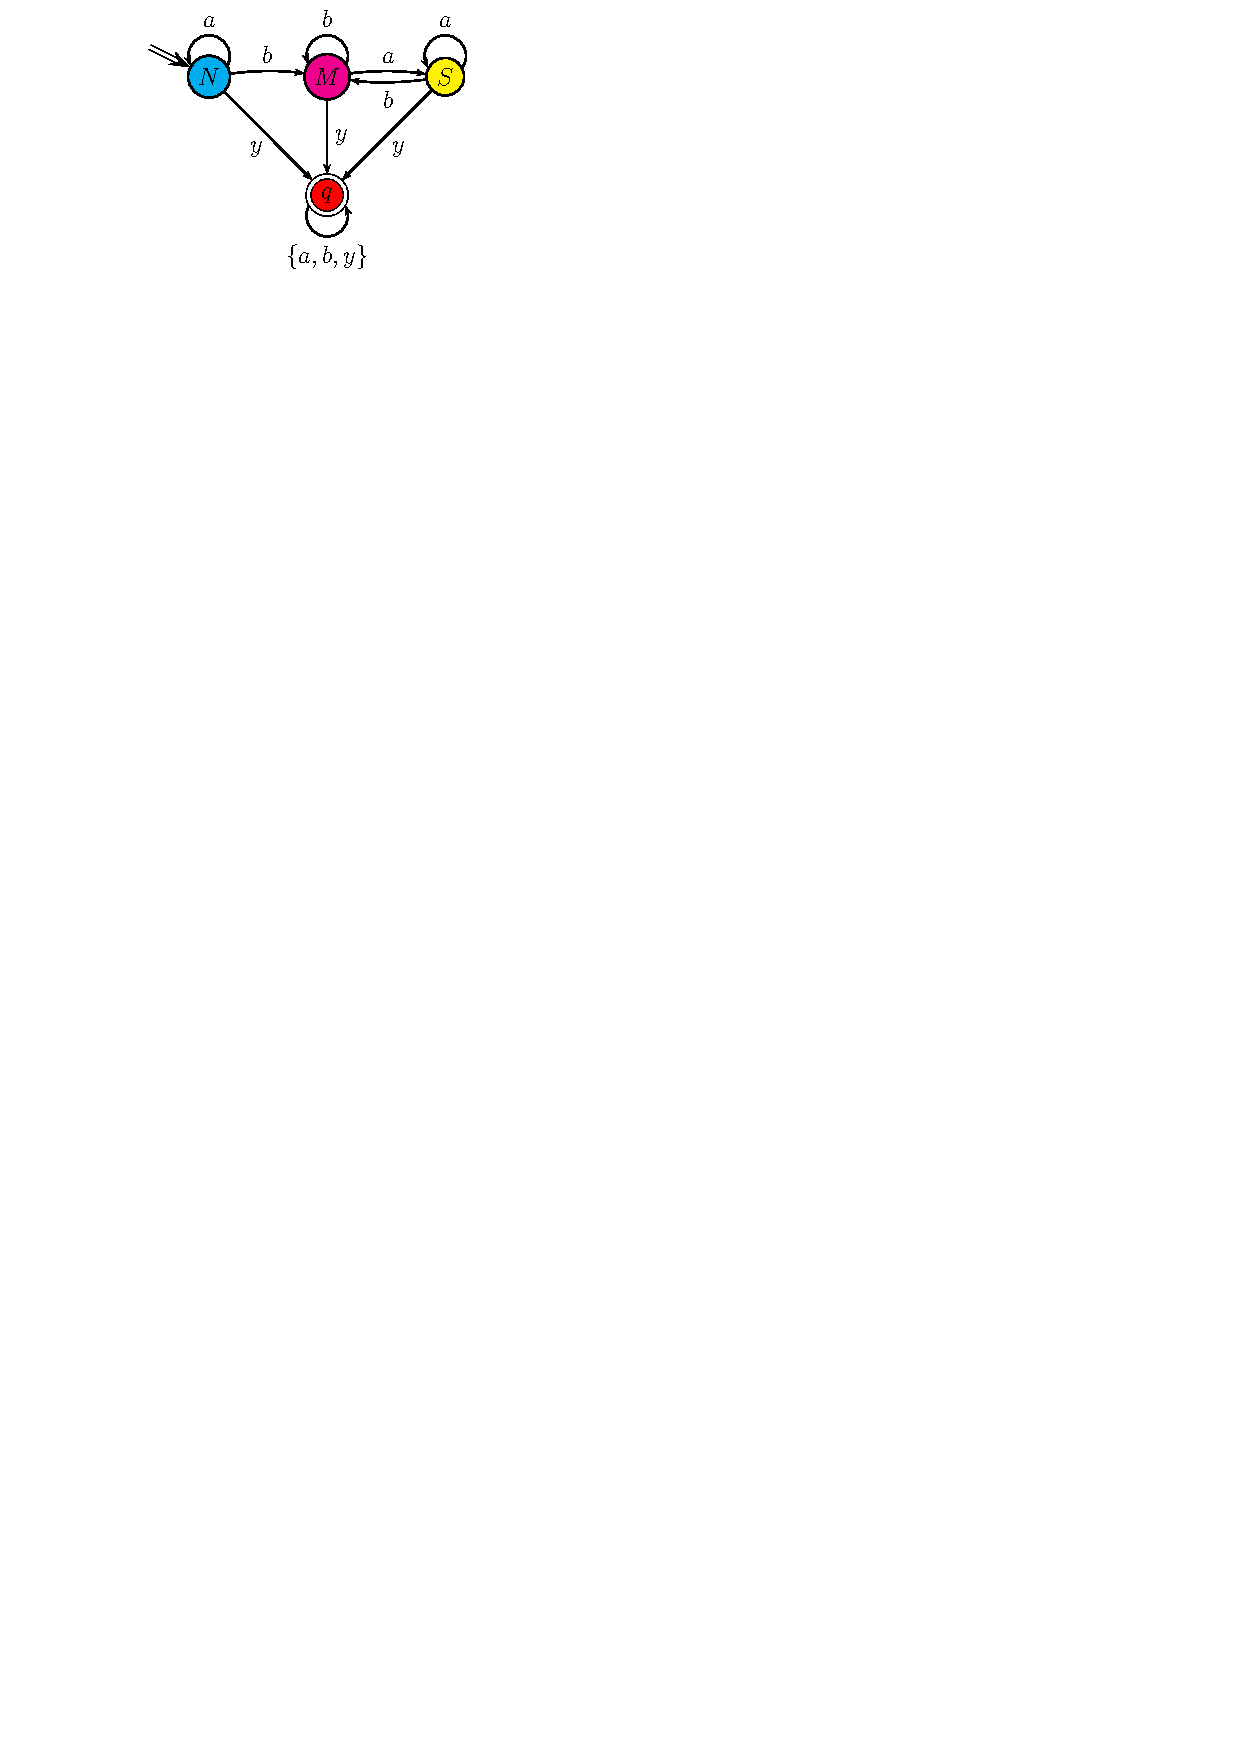
\includegraphics[bb=0 0 160 130]{images/pst.pdf}
\\ \kuti{\label{kuti:pstricks} \Y{PSTricks}による状態遷移図の描画} \\
{\small この状態遷移図を描くのに以下の入力をした.}\\
%「何かの状態遷移図に似てるよなぁ,あぁ TeX のあれかぁ」とかね.
\begin{InText}
%\usepackage[dvips]{graphicx,color}
%\usepackage{pst-all,pstcol}
\begin{TeXtoEPS}
\begin{math}
 \rput(0,3.5){\rnode{root}\relax}
 \cnodeput[fillstyle=solid,fillcolor=cyan](1,3){N}{N}
 \cnodeput[fillstyle=solid,fillcolor=magenta](3,3){M}{M}
 \cnodeput[fillstyle=solid,fillcolor=yellow](5,3){S}{S}
 \cnodeput[doubleline=true,fillstyle=solid,fillcolor=red](3,1){Q}{q}
 \psset{arrows=->,labelsep=3pt}
 \ncarc{N}{M}   \Aput{b}
 \ncarc{M}{S}   \Aput{a}
 \ncarc{S}{M}   \Aput{b}
 \ncline{N}{Q}  \Bput{y}
 \ncline{M}{Q}  \Aput{y}
 \ncline{S}{Q}  \Aput{y}
 \ncline[doubleline=true]{root}{N}
 \nccircle{->}{N}{10pt} \Bput{a}
 \nccircle{->}{M}{10pt} \Bput{b}
 \nccircle{->}{S}{10pt} \Bput{a}
 \nccircle[angleA=180]{->}{Q}{10pt} \Bput{\{a,b,y\}}
\end{math} 
\end{TeXtoEPS}
\end{InText}
\end{center}
\end{figure}
%
%
%
%\begin{figure}[htbp]
% \begin{center}
%
%\\ \kuti{明度と彩度の相関\label{kuti:meisai}}  \\
%{\small 明度とはどれだけ白に近いかという値で、
%黒の明度を0とし、白の明度を1として考えることが多い。
%彩度とは赤や青などの波長がどれだけ強いかを表す
%値で原色の赤の彩度を1とすると赤を含まない灰色の
%彩度は0になる。彩度を持たない色は無彩色と呼ばれている。}
% \end{center}
%\end{figure}

\makeatletter
\renewcommand{\theenumi}{\@arabic\c@enumi}
\makeatother



%
\frontmatter%
%\listofchapter%      章目次
%#!platex jou.tex
\chapter{�ޤ�����}\chaplab{preface}

%\begin{abstract}
%\TeX �Ȥ����ץ���������ʪ������Ǥ���Ȥ��������ɤ���������ߤ����Ǥ���
%\end{abstract}

\newcommand*\kugiri{\bigskip}

\section*{����ϲ��Τ�����ܤ�}

\zindind{ʸ��}{�μ�ɮ}
\indindz{��ݡ���}{�ʳص��ѷϤ�}
\indindz{��ʸ}{�ʳص��ѷϤ�}
���餫��\Z{ʸ��}��ɮ����Ȥ��ˡ��ޤ�\kenten{����}�񤯤٤����Ȥ������Ƥ˴ؤ���
�ͤ���Ȼפ��ޤ������������񤯤٤����Ƥ���ޤä��Ȥ��Ƥ�\kenten{�ɤΤ褦��}
�񤯤���ɬ�������ޤ꤭�ä���ΤǤϤʤ��Ȼפ��ޤ��������礭��ʸ��Ǥ��ä�
�ꡤ���������̤˴ޤ�褦�ʤ�ΤǤ���С�������������Ū����ˡ�����������
�Ǥ��礦���ä˲ʳص��ѷϤΥ�ݡ��Ȥ���ʸ��ɮ�������ͤ���ȡ��������
%��������Τ�Ȥä���������������夹��Ǥ��礦�����Τ褦�ʾ����ǹ����Ȥ�
��������ˡ���Ѥ�����������������夹��Ǥ��礦�����Τ褦�ʾ����ǹ����Ȥ�
��Ƥ���Τ� \ruby{\LaTeX}{��ƥĥ�} �ȸƤФ��ץ������Ǥ���

\indindz{ʸ��}{�κۤ����ä�}
�����ܤǤ� \LaTeX ���Ѥ���ʸ������ˤĤ��Ʋ��⤷�ޤ���\LaTeX ��
\ruby{\TeX}{�ƥĥ�} �ȸƤФ��ץ������ξ�˹��ۤ���Ƥ��륷���ƥ��
����\laTEX �ϥե꡼�������Ǥ��ꡤï�Ǥ�̵���Ǽ�ͳ (\emph{free}) ������
���������ǽ�Ǥ���\LaTeX �򤦤ޤ��Ȥ����ʤ��С�\Z{�κ�}�����ä�����
��ʸ�񤬴�ñ�˺����Ǥ���褦�ˤʤ�ޤ���

\zindind{ʸ��}{��������¤}
\zindind{��}{�����Ƥ�ʬΥ}
�ʳص��ѷϤ�ʸ���ɮ���Ƥ����������ʤ�Сָ��Ф��ϥ����å��Τ� 24\,pt��
�Ǥ���Ȥ���1�Ԥ�ʸ������ 40 ʸ���� 1 �ڡ����� 36 �ԡפȤ����ͤ�\Z{��}��
�ؤ�������Ϲͤ��ʤ������ɤ����⤢�ꡤ\LaTeX �ǤϤ��줬��ǽ�Ǥ���
\LaTeX �Ǥ�ʸ���������¤�˵���Ĥ��ʤ��鸶�Ƥ�ɮ��������Ǥ��뤿�ᡤ
�񼰤����Ƥ�ʬΥ���������ǽ�ʤΤǤ�\footnote{\Z{HTML} \& \Z{CSS}��\Z{XML}
\& \Z{XSL}�Τ褦�ʴط��Ȼ��Ƥ���Ȼפä��ɤ��Ǥ��礦��}��

\zindind{�κ�}{��Ĵ��}
�ܽ������ \LaTeX ��Ȥä������ʤ��ͤ��оݤˡ����Ǥ�ɬ�פȤ����񼰤�
���äƤ����ʳ�\footnote{���Ū���Ϥ��礭�ʳز����Ǥ���С���ʸ��Ƥˤ���
�� \LaTeX �ν񼰤��󶡤��Ƥ���꤬��¿������ޤ���������ζ��鵡�ؤǤ�
\LaTeX �Ѥγذ���ʸ�Υ���������󶡤��Ƥ����⤢��ޤ���}�ǡ���ݡ��Ȥ�
��ʸ����ʸ��� \LaTeX ���Ѥ��ƤɤΤ褦�˼�ɮ���뤫����⤹��Τ���Ū�Ȥ�
��ޤ�\footnote{�κۤ�Ĵ������Ȥ����Τϡ�����ʤ�м�ɮ�Ԥ�ô��������ʬ
�ǤϤʤ�����Ƥ���������Ԥ��٤���ȤǤ����顤�κ�Ĵ���˴ؤ��������ϱ�
�޽���Ū���ΰ��α��Ƥ��ޤ���}��

�����ܤ�ñ�ˡ�\LaTeX �Ȥ����ץ������ε�ǽ��Ҳ𤷤�\kenten{������}�פ�
��������%\footnote{�֤Ǥ�������ץ��꡼���Ȥ����Τ϶���Ū�ʼ�硦���
%����ˡ������������Ƥ��餺�����θ���Ū�ʹ�¤�˴ؤ�������ؤθ��ڤ�����
%���ʤ��Ȥ����Τ�����Ū��������λѤ��Ȼפ��ޤ������Τ褦��������ɬ�פʤ�
%�ȤϻפäƤ��ޤ��󡥤����ޤ����˴ؤ����������ª���Ƥ��ޤ���}
����ư�������Ȥ����򤷤� \LaTeX ��Ȥ����ʤ������
\kenten{���ʽ�}�פ˶ᤤ�Ȼפ��ޤ�%\footnote{���Τ����\Z{�����ƥ饷��}
%����פΤ褦����عֵ��ǽ�ʬ���ѤǤ������Ƥ˶ᤤ�ȻפäƤ��ޤ����������
%���뤿��Υץ�ߥƥ��֤ʼ��ʤϡ����󵻽Ѥ�������ȯã���Ƥ�ʹ֤�Ǿ��ʸ��
%����ܤȤ������Τˤ�����Ť������㥳���Ȥdzμ¤���ˡ���ȡ���ϻפäƤ���
%���������ܤ�ʸ������ܤȤ�������򴹡�ʸ��ɽ��ǽ�ϡˤδ��äȤʤ���ʬ���߼��
%�褦�����Ϥ��Ƥ��ޤ���}
���򺣤� \Z{tips}���Τ褦�������񤬽������줬���Ǥ�
�������Τ褦��������Ǥϼ��Ϥ�������褹��ǽ�Ϥγ����䡤���ʤ������ظ���
�����ƥåץ��åפ��񤷤��Ȥ���¦�̤�����ޤ���
%
%\TeX �� \LaTeX �ϲ�������κƸ����������餷������Ȥ���ʸ���������¤��
%���ΤǤ���Ȥ������������˻Ȥ��륷���ƥ�ǤϤʤ��Ȼפ��ޤ���
\TeX �� \LaTeX �ϲ�������κƸ����������餷������Ȥ���
ʸ������Τ�������¤������������˸�Ψ�褯�б����뤿�������
�Ȥ��륷���ƥ�ǤϤʤ��Ȼפ��ޤ���
\zindind{�ե�����}{������}%
\zindind{����ѥ���}{�β��}%
%
%ʸ�Ϥ���̤˹����������\Z{ʪ��Ū����}��\Z{�ǡ�����}��\Z{��§�黻}��
%\Z{�������������}���ե����������ϡ��ץ������ι�®�����Τ������������
%��Ŭ������٥�θ������Ȥȥ���ѥ������ˤĤ������򤹤�����Ǥ��ޤ�
%
�ܽ������٤����Ƥ˴ؤ��Ƥϡ����Ԥ������֥ڡ����Ǹ������Ƥ�
��ع�������\LaTeXe�٥��꡼���򻲾Ȥ��Ƥ�������\footnote{%
\webThorTypo}��\genzai ¿����³�Ԥ�̤���Ǥ���������ʳ���ʸ����
��Ū�˸������Ƥ��ޤ���



\section*{����}

\index{����}
�ܽ�Ǥ�\Z{����}���ѹ�������ˤ�ä�Ʊ�����Ǥ�
��ä���̣����Ĥ�Τ�¿������ޤ���\qu{\prog{dvipdfmx}}
�Ȥ����줬���ä��Ȥ��Ƥ�\qu{\textsf{dvipdfmx}}��\qu{\texttt{dvipdfmx}}��
\qu{\textsl{dvipdfmx}}��\qu{\textit{dvipdfmx}}�Ϥ��٤��̤ΰ�̣��
���äƤ��ޤ���\zindind{����}{�μ���}�����ν��Τμ���ˤĤ��Ƥ�
\secref{font}�򻲾Ȥ��Ƥ���������
\begin{center}
\zindind{�����ܡ���}{���������}%
 \begin{tabular}{lll}
 \TR
 \Th{����}          & \Th{��̣}      & \Th{��} \\
 \MR
 �����ޥ���    & �̾��ʸ��& \textrm{dvipdfmx}\\
 ���󥻥����  & �ѥå������䥯�饹\pp{\secref{class}����}& \textsf{dvipdfmx}\\
 �����ץ饤����& �����ܡ��ɤ�������Ϥʤ�& \texttt{dvipdfmx}\\
 ������å���  & �ѿ��䶯Ĵ& \textit{dvipdfmx}\\
 ��������    & ���ץ����\pp{\secref{classopt}����}& \textsl{dvipdfmx}\\
 \BR
 \end{tabular}
\end{center}

��ʸ��Ǻ�¦�˥����ץ饤���Ρ���¦�ˤ���˽स�������㤬
�����Τϡ������Ϥ��Ф�ɽ���ޤ���
\par\addvspace{3.0ex plus 0.8ex minus 0.5ex}\vskip-\parskip%
\hspace*{\IOm}\hspace*{-1ex}%
\makebox[0pt][l]{%
  {\begin{minipage}[c]{.47\fullwidth}\small%
\begin{ttfamily}%
The length of a pen should be\\
comrotable to write with: too\\
long and it makes him tired;\\
too short and it\cmd{ldots}.%
\end{ttfamily}%
  \end{minipage}%
  }\hspace{0.05\fullwidth}%
  {\begin{minipage}{.47\fullwidth}%
      \begin{trivlist}\item\small%
The length of a pen should be comrotable
to write with: too long and it makes him
tired; too short and it\ldots.%
   \end{trivlist}%
   \end{minipage}}}%
\par\addvspace{3.0ex plus 0.8ex minus 0.5ex}\vskip-\parskip%

\Z{�ƥ����ȥ��ǥ��å�}�ʤɤ�Ȥ������ƥե�����Ǻ�¦�Τ褦�����Ϥ���ȡ�
��¦�ν������Ʊ���褦�ʷ�̤��ǧ�Ǥ��ޤ���

��ʸ�������������Ф��Ƥϡ�����į���ΤǤϤʤ����ºݤ˼�ʬ�����Ϥ���
�¹Է�̤��̣���Ƥߤ���򤪴��ᤷ�ޤ���

�ʤ��¹Է�̤��̣������򴫤��Τ�������ϥ���ԥ塼���ץ������
�Ȥ����Τ�¾��ʬ�����٤�ȸ��ݤκƸ���������Ū�Ǥ��ꡤ�ɻ��ǽ����
�⤤�Ȥ������ˤ���ޤ�\footnote{�����ؼ¸��Τ褦���︳�Ԥ򽸤��ɬ������
����ޤ��󡤶��餯�������٤ν���ǽ�Ϥ�ͭ����׻��������椢��н�ʬ�Ǥ���}��

�ʳ�Ū�����Ҥ��濴�ξ��ϡ����򤬤ʤ���п��ѤǤ��ʤ��פȤ����Τ��ڤǤ�
��������ԥ塼���ץ������ξ��ϡ��ºݤ˼��Ȥäƥץ��������Ȥ��
�ߤơ�����ѥ��뤷���¹ԡʼ¸��ˤ�����̤��̣�ʹͻ��ˤ������ï�Ǥ�
��ͳ�ˤǤ��ޤ��ʤ��Υץ������Υ����������ɤ��輨����Ƥ���¤�ˡ�
����˿��ؤξ����Τ褦�ˡ����르�ꥺ��Ū���äϰ��ټ�ʬ�Ǥ��ι�¤�ȸ�����
�ͤ��ƥץ�����ह��С�%Ŭ�ڤʲ�᤬�Ǥ���褦�ˤʤꡤ��������޴���Ȥä�
����줿�μ��ϰ������οͤΤ�Τˤʤ�ΤǤ������Τ褦�ʹͤ��˴�Ť�����
��Ǥ�����濴���ä�ʤ�Ƥ���Τǡ��������ʬ�����Ϥ�������ˤϤ��μ�
�Է�̤��̣�������侩���ޤ���

\kugiri

ʸ��ˤ�����\type{which perl}�Ȥ���ɽ����\Z{���ޥ�ɥץ���ץ�}��
\Z{������}�ʤɤ�\Z{���󥽡���}��������Ϥ򼨤��ޤ���
ʣ���Ԥ����Ϥξ��ϼ��Τ褦�ˤ��Ƥ��ޤ���

\begin{InTerm}
 \type{platex input.tex} 
 \type{jbibtex input.tex} 
 \type{dvipdfmx -S -o output.pdf input.dvi}
\end{InTerm}

\index{"$@\verb+$+!���󥽡����\zdash}%"
��Ƭ�Υɥ�`\str$'�ϥ��󥽡����ɽ������Ƥ��뵭��ǡ�
�桼�������Ϥ��ޤ���

\kugiri

\Z{�����ܡ���}��������\Z{�����ȥå�}�򲡤����򼨤��ˤ� \key{Alt} ��
�褦�ˤ��Ƥ��ޤ���\key{Ctrl,Alt,Delete} �� \key{Ctrl}��\key{Alt}��
\key{Delete} ������Ʊ���˲������ˤʤ�ޤ���\key{Ctrl,x}\key{Ctrl,s} �� 
\key{Ctrl,x} �򲡤������ \key{Ctrl,s} �򲡤�����ɽ���ޤ���

\kugiri

�ܽ��ɽ������Ƥ���\Z{�Хå�����å���}`\bs'��Windows�Ķ��ˤ�äƤϡ�
�ƥ����ȥ��ǥ��å����DZߵ���`\yen'�Ȥ��ƻ�ǧ�Ǥ���Ȼפ��ޤ���Windows
�桼�������ϴ���Ū��`\yen'��\unixos �Ǥ�`\bs'��ʸ���������Ƥ����ǧ��
����ĺ�������ꤢ��ޤ���

\kugiri

\index{�ѿ�}
���餫��ʸ�������ͤ��֤�������Τ�\va{�ѿ�}�Τ褦��
ɽ�����Ƥ��ޤ���

\kugiri

\begin{Trick}
\begin{normalsize}
  ���������Ȼפ���սꡤ\LaTeX ��ư����˿���Ƥ��������
 �ؤ��Ƥϡ���������Τ褦�ˡصޥ����֤���������٤�\textdbend
 �ޡ�������Ϳ���Ƥ��ޤ���
\end{normalsize}
\end{Trick}


%\begin{comment}

\section*{�ե꡼�������Ȥ�}

{\LaTeX}�ϥե꡼�������Ǥ������ν��פʥޥ˥奢��ϥե꡼�ǤϤ���ޤ���
{\LaTeX}�ץ��������ȥ��С���\Person{Michel}{Goossens}��
\Person{Sebastian}{Rahtz}��\Person{Frank}{Mittelbach}��
\Person{Leslie}{Lamport}�餬���Ǥ��Ƥ���ޥ˥奢������ܸ�����1��5,000��
���٤����ʤǤ���������{\LaTeX}�桼����ɬ�ȤȤ����Ƥ�����Ҥ�4������
��ޤ���

\begin{itemize}
\item \wasyo{\LMANUAL}\cite{latexbook}\quad 3,000�ߡ�
\item \wasyo{\COMP}\cite{latexcomp}\quad 4,800�ߡ�
\item \wasyo{\GCOMP}\cite{graphicscomp}\quad 5,400�ߡ�
\item \wasyo{\WCOMP}\cite{webcomp}\quad 4,800�ߡ�
\end{itemize}

\yo{ɬ�Ȥ��ܤ���ä���18,000�ߤ⤫����Τ�}�Ȼפ�����Ǥ��礦��
����Ǥϥե꡼������������ȤäƤߤ褦�Ȼפä����䡤ï����������ƻȤ�
�Ϥ᤿���ϼ��Ф��Ť餤�ΤǤϤʤ����Ȼפ��ޤ����ޤ���{\LaTeX}�λȤ�����
���뵻�ѻ��������Ƹ�������Ƥ��ޤ��Τǡ����ڤ����������֥ڡ����ʤɤǾܤ�
����갷�äƤ����礬����ޤ������Τ褦�ʥڡ����򸫤���ä˺�����Ϥ�
���Ȼפ��ޤ���������Υ��Υ���¸�ߤ���Τǡ��ɤ��⾡�꤬�����褦�Ǥ���

\Person{Richard}{Stallman}���ʤ����̤ꡤ���줬�ե꡼��������������������
�ǤϤʤ����Ȼפ��ޤ��������ǿ����˥ե꡼�ʥޥ˥奢������������ˤ���
������������{\LaTeX}�δ�¸�Υޥ��������饹�ʤ�Ӥ˥ץ������γ�����ˡ��
�Ĥ��Ƥ��ä˸��ꤷ�ޤ�����̳Ū�ʽ���κ����ǤϤʤ���˥�ݡ��Ȥ���ʸ���
������ξ���򽸤�Ƥ��ޤ��Τǡ�ɽ�˿����դ������Ȥ����ե���Ȥˤ������
�����Ȥ�������ϴޤ�Ǥ��ޤ��󡥤���˥ޥ��������饹�κ�����ˡ�ϺǾ��¤�
�Ȥɤ�Ƥ��ޤ��Τǡ���¸���ɽ��\appref{info}���黲�Ȥ��Ƥ���������

%\end{comment} 

% まえがき
%#!platex jou.tex
\chapter{�ռ�}

�ܽ��������뤿��ˤ�����¿���������Τ����ϡ����������ʤ���м¸���
�񤷤��ä������ưפ������Ǥ��ޤ���

�ޤ�{\TeX}�κ�ԤǤ���\Person{Donald}{Knuth}�ˤϺ���δ��դ�ɽ���ʤ����
�ʤ�ޤ��󡥻᤬\TeX �Ȥ���������äƤ��줿�����ǡ�����ʤˤ������餷
���������θ���������Ǥ������˴�Ӥ򴶤��Ƥ���ޤ���%��ʸ��Ū�ץ�����ߥ�
%���٤ȸƤФ��褦�ˡ��ץ�����ߥ󥰤Ȥ����԰٤��Τ�Τ�ݽѤΰ�˹�ᡤ
%�����

{\LaTeX}���̤˴ؤ��Ƥ�\Hito{����}{���}��\Hito{��¼}{��ɧ}��\Hito{��
¼}{����}��\Hito{�ȱ�}{Ű��}���¿���λ���ؤӤޤ��������ǡ��������ǥ�
����ʤɤ˴ؤ��Ƥ�\Hito{��¼}{���}��ꤴ�����򤤤��������ꡤ�ޤ����Ҥ�
�ߤ���ĺ���ޤ�����

{\LaTeX}�κ�ԤǤ���\Person{Leslie}{Lamport}��
{\LaTeXe}�γ�ȯ�򤵤줿\Person{Frank}{Mittelbach}��
\Person{Johannes}{Braams}��\Person{David}{Carlisle}��\Person{Michael}{Downes}��
\Person{Alan}{Jeffrey}��\Person{Sebastian}{Rahtz}��\Person{Chris}{Rowley}��
\Person{Rainer}{Sch\"opf}��
{\TeX}�����ܸ첽�򤷤Ʋ����ä�\Hito{����}{��}�ȥ���������������
Windows��{\pTeX}��ܿ����Ƥ������ä�\Hito{��ƣ}{μ}��
\Dviout ��ȯ���줿\Hito{����}{��ͺ}��\Hito{����}{����}��
\prog{\BibTeX}�γ�ȯ�򤵤줿\Person{Oren}{Patashnik}��
\prog{MakeIndex}��ȯ�����ɤ��줿\Person{Pehong}{Chen}��\Person{Nelson}{Beebe}��
\Dvipdfm �κ�ԤǤ���\Person{Mark}{Wicks}��{\Dvipdfmx}���ݼ顦�����򤵤�Ƥ�����
\Hito{ʿ��}{�Ӻ�}��\Hito{��}{����}��{\PS}��PDF�ʤɤΥڡ������Ҹ�
���������줿Adobe�Ҥ�����������ˡ��ե꡼���������ޥ����ѥå������ʤ�
�κ����ǡ�{\TeX}��ʬ��ˤ����ƹ׸����줿�����ˤⴶ�դ������ޤ���

\hito{��ͧ}{����}��\hito{����}{����}�ˤ��ܽ�θ������Ŧ���Ƥ�����������
��˲������٤��ս�ˤĤ��Ƶ������Ƥ��������ޤ�����
\hito{����}{����}�ˤϥɥ��ĸ�ɽ���ˤĤ��ƶ����Ƥ��������ޤ�����

¿�����������ܽ�κ����˹׸����Ʋ������ޤ����������ˤ��꤬�Ȥ��������ޤ���
���Ϥ��Ƥ������ä������Τ���ˤ⡤�ܽ����ܤ� \TeX ���ߥ�˥ƥ��ˤ�����
����Ū�ʺ⻺�Ȥ��ƻĤ�³��������ڤ�˾��Ǥ���ޤ���

\clearpage
\thispagestyle{empty}
\null\vfill

\index{GNU!\zdash FDL}
\centerline{\headfont 
  �����ܤ� GNU FDL��ȯ�Ԥ���Ƥ��ޤ�! �����������Ƚ���\ldots.}

�ܽ�� \fdl\footnote{FSF �ˤ��ե꡼��ʸ������Ѥ˴ؤ���
�饤���󥹤λ��Ǥ���}�ν��ҤǤ����顤���θ��Ƥ�PDF�Ǥ����ԤΥ����֥ڡ���%
\footnote{\webThorTypo}�Ǹ������Ƥ��ޤ���
��������������­����˴ؤ��������갷�äƤ��ޤ�\footnote{��̾��
�ع�������\LaTeXe ����ԡ٤Ȥ���̾���Ǹ������Ƥ����礬����ޤ���}��
%
�ܽ�ȡ�Ʊ���褦�ʽ��Ϥ� \LaTeX �Ǽ¸��������פȴ������Τ�
����С�ľ�ܸ��Ƥ򻲾Ȥ��ƤߤƤ���������

�ܽ�ΰ����Ѥ� PDF��\Y{hyperref}�ˤ������������ǽ�ʱ����� PDF ���
�����Ƥ��ޤ����ѥ�����ʤɤ˱����� PDF ����¸���Ƥ�����ʸ���󸡺���Ǥ�
�ޤ����������Τ��ܽ񤬤ʤ����ˤ���ѤǤ����ΤȻפ��ޤ���

�Ǹ��\gnu �λ���\footnote{����\ruby{\gnu}{�̡�}�˴ؤ�������������Ƥ�
�����Τ�FSF: \emph{Free Software Foundation} (gnu@gnu.org) �ȸ���
�ޤ�����餬�ܻؤ��Ҳ����λ��ۤξܤ������ˤĤ��Ƥϥ����֥ڡ���
(\webGNU) �˥�������������ɤ��Ǥ��礦���䤬�ܽ���ä����ä����⡤����
FSF�γ�ư�˿�ȯ���줿��ΤǤ�����̣������ޤ����餴������������}��
\fdl ��������Ƥ��줿 \emph{Free Software Foundation} ��
\Person{Richard}{Stallman} �˴��դ��ޤ���



%   謝辞
%#!platex jou.tex
\chapter[�ե꡼���եȥ������ȥե꡼�ޥ˥奢��]
   {{\huge �ե꡼���եȥ������ȥե꡼�ޥ˥奢��}}\chaplab{free}
\markboth{�ե꡼���եȥ������ȥե꡼�ޥ˥奢��}
{�ե꡼���եȥ������ȥե꡼�ޥ˥奢��}

\begingroup
\small
%\setlength{\evensidemargin}{\oddsidemargin}
%\setlength{\textwidth}{\fullwidth}
%\setlength{\linewidth}{\fullwidth}
\begin{multicols}{2}

�ե꡼�ʥ��ڥ졼�ƥ��󥰥����ƥ�ˤ��������η�٤ϡ����եȥ�����������
�ǤϤ���ޤ���\zdash �䤿���������Υ����ƥ�˴ޤ�뤳�Ȥ���ǽ�ʡ��ե꡼����
���ʥޥ˥奢�뤬��­���Ƥ��뤳�Ȥ���������ʤΤǤ����䤿���κǤ���פʥ�
��������¿���ϡ������ʥޥ˥奢��ȶ����󶡤���Ƥ��ޤ��󡣥ɥ������
�Ϥ����ʤ륽�եȥ������ѥå������ˤ����Ƥ�ɬ���Բķ�ʰ���ʬ�Ǥ����顢��
�פʥե꡼���եȥ������ѥå��������ե꡼�ʥޥ˥奢��ȶ����󶡤���ʤ���
��С�������礭�ʷ�٤Ǥ����䤿���Ϻ��������Τ褦�ʷ�٤��¿�������Ƥ�
�ޤ��� 

�Ρ�����ǯ�����Τ��Ȥˤʤ�ޤ�����Perl ��ؤܤ��Ȼפä����Ȥ�����ޤ���
��ϥե꡼�ʥޥ˥奢���������ꤷ���ΤǤ���������϶ˤ���ɤߤˤ������
�Ǥ�����Perl �桼�������������ʤˤĤ���ʹ���Ƥߤ��Ȥ��������Ϥ���ɤ�
�����ѥޥ˥奢�뤬����ȶ����Ƥ��줿�ΤǤ����������������ϥե꡼�ǤϤ�
��ޤ���Ǥ����� 

����Ϥɤ����Ƥ��ä��ΤǤ��礦? �����ɼ��ʥޥ˥奢������Ԥ����ϡ��ޥ˥�
������ O'Reilly Associates �ҤΤ���˽񤭡�O'Reilly �Ϥ���������Ū��
���β��ǽ��Ǥ����ΤǤ�����ʣ���Ƕ��ѹ����������ե�����������Բ�\zdash
�������ä����ϥޥ˥奢���ե꡼���եȥ������Υ��ߥ�˥ƥ���������Ф���
���ޤ��ޤ��� 

����Ϥ��μ�ν�����Ȥ��ƤϺǽ�Τ�ΤǤϤ���ޤ���Ǥ����������ơʻ䤿
���Υ��ߥ�˥ƥ��ˤȤäƤ��礭��»���ʤΤǤ����˺Ǹ�Ǥ���Ȥ����줤����
���󡣤��ν�����ʹߤ⡢����Ū�ʥޥ˥奢����ǼԤ����˿�¿�������Ԥ���
�򤽤��Τ��������Υޥ˥奢������¤�ä������Ƥ��ޤ�������ϡ� GNU �桼
���ΰ�ͤ���ν񤤤Ƥ���ޥ˥奢��ˤĤ���Ǯ���˸��Τ��٤�ʹ���ޤ�����
��Ϥ���ˤ�ä� GNU �ץ��������Ȥ����Ǥ���ȹͤ��Ƥ����ΤǤ�\zdash �Ȥ���
�������³���ơ��䤿���������Ȥ����Ȥ��Ǥ��ʤ��褦�����¤�ݤ��Ǥ�����
���ǼԤȤη���˥����󤷤��ȽҤ٤��Τǡ���δ�˾���Ǥ��դ����Τ���Ǥ�
���� 

������Ȥ����Ѹ�ǽ񤯤Ȥ������Ȥϥץ�����ޤδ֤ǤϤޤ�ʥ�����Ǥ����顢
�ޥ˥奢��򤳤����ä����ȤǼ���;͵������̵���ΤǤ��� 

�ե꡼��ʸ�������Ȥʤ�Τϡ��ե꡼���եȥ�������Ʊ�͡���ͳ�Ǥ��ꡢ����
�ǤϤ���ޤ��󡣤����Υޥ˥奢����������� O'Reilly Associates ������
���줿���ԡ���������׵᤹��Ȥ������ȤǤϤʤ��ΤǤ�\zdash ���켫�Τ��̤˹���
�ޤ���ʥե꡼���եȥ��������Ĥ⡢�ե꡼��GNU �ޥ˥奢��ΰ������줿���ԡ�
�����䤷�Ƥ��ޤ��ˡ���������GNU �ޥ˥奢��ϥ����������ɷ����������ǽ��
�Τ��Ф���O'Reilly �Υޥ˥奢��ϻ����ΤǤ�������Ǥ��ޤ���GNU �ޥ˥�
�����ʣ�̤�����ѹ��ε��Ĥȶ����󶡤���Ƥ��ޤ���Perl �Υޥ˥奢��Ϥ�
���ǤϤ���ޤ��󡣤������ä����¤���������Ǥ��� 

�ե꡼�ʥޥ˥奢��Ǥ��뤿��δ��ϥե꡼���եȥ������Τ���Ȥ��ʤ��ɤ�
���Ƥ��ޤ������δ��Ȥϡ����٤ƤΥ桼���ˤ����μ�ͳ��Ϳ����Ȥ�������
�Ǥ����ޥ˥奢��򥪥�饤��ޤ��ϻ����ΤǤ��Υץ������Τ��٤ƤΥ��ԡ�
�Ȱ����󶡤Ǥ���褦�������ۡʾ���Ū�����ۤ�ޤ�ˤ����Ĥ���Ƥ��ʤ����
�ʤ�ޤ��󤷡��ѹ��ε��Ĥ���פǤ��� 

����Ū�ʥ롼��Ȥ��ơ��͡��ˤ���������ʸ�Ϥ���Ҥ��ѹ�������Ĥ�Ϳ��
�뤳�Ȥ�ɬ�ܤ��Ȥϻ��פ��ޤ��󡣽񤫤줿��Τ˴ؤ��������������եȥ���
���Τ����Ʊ���Ǥ���ɬ�פ�̵���ΤǤ����㤨�С����ʤ����ˡ�����ʸ�ϤΤ�
���ʡ���ʬ�ι�ư���Τιͤ�������������������ѹ�������Ĥ�Ϳ������Ǥ��
����ȤϹͤ����ޤ��� 

���������ե꡼���եȥ������Τ����ʸ��ˤȤä��ѹ��μ�ͳ���ʤ����פǤ���
���ˤĤ��Ƥϡ����̤���ͳ������ΤǤ����͡������եȥ��������ѹ����븢����
�ԻȤ��ơ����եȥ������˵�ǽ��ä������ѹ������ꤹ��ȡ���餬�ɿ�Ū�Ǥ�
��Хޥ˥奢����ѹ����褦�Ȥ���Ǥ��礦\zdash ����������������Τ�ͭ�Ѥʥ�
������Ȥ��ѹ����줿�ץ������ȶ����󶡤Ǥ���櫓�Ǥ��������ǡ��ץ���
��ޤ��ɿ�Ū�ˤʤ뤳�Ȥ�Ż��򴰿뤹�뤳�Ȥ�ػߤ��롢���뤤�Ϥ�����Τ�
�����С��ץ��������ѹ�����ʤ���餬�������鿷�����ޥ˥奢���񤭤ʤ�
�����Ȥ��׵᤹��ޥ˥奢��ϡ��䤿���Υ��ߥ�˥ƥ��Υˡ�������������Τ�
�ϸ����ʤ��ΤǤ��� 

����Ū���ѹ��ζػߤϼ���������ޤ��󤬡����������¤��ѹ��μ�ˡ�˲ݤ�
�Ƥⲿ�����������������ޤ����㤨�С������Ԥ����ɽ������¸���뤳��
���׵ᤷ���ꡢ�������۾��������̾�Υꥹ�Ȥ���¸���׵᤹��Τ�OK �Ǥ���
�����ޤ����ѹ����줿�Ǥϡ�����餬�ѹ����줿�Ȥ������Τ�ޤ�Ǥ��ʤ����
�ʤ�ʤ��Ȥ����׵�򤹤�Τ⹽���ޤ��󤷡����������Τκ�����ѹ���ػߤ�
�뤳�Ȥ���⡢�������ä��᤬����Ū�ʥȥԥå��򰷤äƤ��ʤ��¤�����ˤϤ�
��ޤ����GNU �ޥ˥奢��ΰ����Ϥ������ä����ޤ�Ǥ��ޤ��ˡ� 

���μ�����¤�����ˤʤ�ʤ��Τϡ�����Ū������Ȥ��Ƥϡ�����餬�ɿ�Ū��
�ץ�����ޤ��ޥ˥奢����ѹ����줿�ץ������ˤ��碌�Ƽ�ľ�����뤳�Ȥ��
�ᤵ���ʤ�����Ǥ�������������С��������ä����¤ϥե꡼���եȥ������Υ�
�ߥ�˥ƥ����ޥ˥奢������¤˳��Ѥ��뤳�Ȥ�ػߤ��ʤ��ΤǤ��� 

�������ʤ��顢�ޥ˥奢��ε���Ū�����ƤϤ��٤��ѹ���ǽ�Ǥʤ���Фʤ�ޤ�
�󡣤����ơ��ѹ��η�̤򤢤������Ū�ʥ�ǥ��������٤Ƥ��̾�����ͥ�
�����ۤǤ��ʤ���Фʤ�ޤ��󡣤����Ǥʤ�������¤ϥ��ߥ�˥ƥ���˸���ޤ�
�Τǡ��ޥ˥奢��ϥե꡼�ǤϤʤ��������ǻ䤿���ˤ�¾�Υޥ˥奢�뤬ɬ�פ�
�ʤ�ޤ��� 

�Թ��ˤ⡢����Ū�ʥޥ˥奢�뤬¸�ߤ�����ˤϡ��⤦��ĥޥ˥奢����
�Ƥ����ͤ�õ���ΤϺ���ʤ��Ȥ�¿���ΤǤ����㳲�Ȥʤ�Τϡ�¿���Υ桼��
������Ū�ʥޥ˥奢��ǽ�ʬ�ȹͤ��Ƥ��뤳�ȤǤ�\zdash �����ǡ����ϥե꡼�ʥ�
�˥奢����ɬ�פ�ǧ��ʤ��ΤǤ������ϥե꡼�ʥ��ڥ졼�ƥ��󥰥�����
�ब���������٤�����������Ƥ��뤳�Ȥ�ʬ����ʤ��ΤǤ��� 

�ɤ����ƥ桼��������Ū�ʥޥ˥奢��ǽ�ʬ���Ȼפ��ΤǤ��礦? ���ͤ��ϡ���
������ˤĤ��ƹͤ������Ȥ��ʤ��ΤǤ��礦����Ϥ������⤬����������������
�����餫�Ǥ��Ѥ��뤳�Ȥ���Ԥ��Ƥ��ޤ��� 

¾�Υ桼���ϡ�����Ū�ʥޥ˥奢�������Ū�ʥ��եȥ�������������������
��Ʊ����ͳ���������������Τ��ȹͤ��ޤ���������������Ū�ʸ��Ϥ���
�Τ�ʪ����Ƚ�Ǥ�����ͳ����Ȥ���Ŭ�Ѥ��ʤ��ΤǤ����������ä��͡��ˤ���
��ʤ�ΰո�����Ļ�ʤ�����ޤ������������������ä��ո��ϼ�ͳ��ޤޤʤ�
���ͤ������ӽФ��Ƥ����ΤʤΤǡ����ϼ�ͳ��ɾ������䤿���δ��Τ��
�ɤ����ȤϤʤ����ޤ��� 

��������ˤĤ��Ƥ��ä򹭤�Ƥ����������䤿���ϥޥ˥奢�������Ū�ʽ��Ǥ�
����˼���³���Ƥ��ޤ����⤷�䤿��������Ū�ʥޥ˥奢��Ͻ�ʬ�Ǥ�̵���Ȥ�
�����ۤ򹭤��ʤ�С������餯 GNU ��ʸ���񤯤��Ȥǽ��������Ȼפ�����
�ͤϼ��٤�ˤʤ����ˡ���餬������ɤΤȤ����ե꡼�ˤ��ʤ���Фʤ�ʤ�
�Ȥ������Ȥ���Ǥ��礦�� 

�䤿���Ϥޤ�������Ū���ǼԤ��Ф��ơ�����Ū�ʥޥ˥奢������äƥե꡼��
���ԡ���եȤμ�ĥ�����ޥ˥奢������䤹�뤳�Ȥ�����Ƥ��ޤ������ʤ���
����ư�������Ǥ����Ĥ���ˡ�ϡ��ޥ˥奢����㤦���ˤ������۾��������
���������ԡ���եȤʥޥ˥奢����󥳥ԡ���եȤʤ�Τ��⹥����㤦�Ȥ�
�����ȤǤ��� 

\begin{center}
 Copyright \textcopyright\ 2000 Free Software Foundation, Inc., 59
 Temple Place - Suite 330, Boston, MA 02111, USA
\end{center}


��ʸ�˰����ѹ���ä������������ɽ����Ĥ��¤ꡢ ����ʸ�����ΤΤ�����
�����Τˤ�����ʣ����������ۤ���Ĥ��롣

\end{multicols}

\endgroup

%\clearpage

\section*{Free Software Foundation�Ȥ��γ�ư�Ĥ���}

���ҤΡإե꡼���եȥ������ȥե꡼�ޥ˥奢��٤�\emph{Free Software
Foundation}��\Person{Richard}{Stallman}�ˤ�äƽ񤫤줿�����֥ڡ�����
\Hito{Ȭ��}{����}\footnote{mhatta@gnu.org}������������ΤǤ�������
\ruby{GNU}{�̡�}�˴ؤ���ʸ�Ϥ�������Ƥ������Τ�FSF: \emph{Free Software
Foundation}\footnote{gnu@gnu.org}�ȸ����ޤ�����餬�ܻؤ��Ҳ����λ�
�ۤξܤ������ˤĤ��Ƥϥ����֥ڡ���\footnote{\webGNU}��
��������������ɤ��Ǥ��礦���䤬�ܽ���ä����ä����⡤����FSF�γ�ư��
��ȯ���줿��ΤǤ����顤��̣������ޤ����餴������������

% title: \emph{The Design Philosophy of Hermann Zapf}
% author: \Person{Hermann}{Zapf}
% ISBN:  4-947613-15-7
% year: 1995 {\textcoyright} Robundo
% ���ܤˤ��ƻ�Ȥ���ʪ�����롥��Ȥ������������ɽ�����졤���ηݽ�������
% ��ɾ������Ƥ��롥���ΤǤ�����Ū���ͤ�ǧ�Τ���Ƥ��ʤ���礬���롥

\index{GNU!\zdash FDL}
������󡤤����ܤ� GNU FDL\footnote{FSF �ˤ��ե꡼��ʸ������Ѥ˴ؤ���
�饤���󥹤λ��Ǥ���}��ȯ�Ԥ���Ƥ��ޤ��������Ƚ���\ldots.

\begin{comment}

\section*{���뤤�ӥ��ͥ��ޥ�����פ򲣼�ꤵ���������}

%\begin{metacomment}
% ����Ҳ�ǽ��ǤȤ���ƻ��é�뤿��ˤϡ����ǼҤȤ������ʷ���򶯤�����
% ��礬¿�����ºݡ������������������Ͻ��ǼҤ˰���Ū�˷���졤������
% ���ڡ������ⲿ�⤫����ǼҤ���ƳŪ�˲����դ��륱������¸�ߤ����������
%\end{metacomment}

���뤤�ӥ��ͥ��ޥ�˼�ʬ������ʪ�����פ򲣼�ꤵ���������ˤʤäƤ���
�ΤϤɤ����Ƥ�������ϲ����⾰����ͳ���㤨�и������ŤȤ��Ҳ�Ū��ư�Ȥ�
����Τˤ�餺��������פ��ӥ��ͥ��ޥ��ư�����Ƥ��뤫���¾�ʤ�ʤ���
��ɤ����פ��ߤ��������������ʪ����Ǥ����Ƥ���ΤǤ��롥�Ҳ�Τ����
���Ƕ�̳���Ѷ�Ū�˹ԤäƤ���ΤϾ����Ǥ��롥���ǤȤ����ΤϤ������٤Υ�
������ȼ�����ܤ����ʤ���м����ϸ��롥����ϸ��¤Ǥ��롥�����ܤ��
�Ǥ��ʤ�����äˤʤ�ʤ���

�Τ�����ݸ����ˡ�Ȥ����ΤϤ����ƴ�ñ�ʤ�Τ��ä��������ꡤ���Ρ�
�桤�Ͱ��ʤɤ������Τ�ʪ��Ū�ݸ�˷�ӤĤ��Ƥ���������Ҳ�ǤϤ��Τ�
����ʪ��Ū�ݸ��ɬ������ͭ���ǤϤʤ����Ż����ΤǤ���п��ä��Ҥ��դ�����
���⤢�롥����ˤ�äƼҲ�ϤɤΤ褦�������˸������٤����������Ż�����
�ˤ��Żҽ�̾���Ż�Ʃ���������ԡ��ץ��ƥ��Ȥ�ܤ����ɤ��Τ���������
��Ϥ��Τ褦���ݸ�򤷤Ƥ�ۤȤ�ɤξ��ϥ��������ä��˽�����������
�ͤ��Ƥ��롥���¡�CD-ROM/DVD-ROM���Υ��ԡ��ץ��ƥ��Ȥ⵻��Ū�μ��Τ�
��ͤ��������ݸ����򤹤�褦�ʼ�ˡ��ͤ������Ƥ��뤷���ݸ��̵���ˤ�
��褦�����֤⽼�¤��Ƥ��롥

�Ҳ����Τ���¤Ū��ʸ����ư��˾��ΤǤ���С�������ȤǤϤʤ���̱�֤�
��������Τ��������٤��Ǥ��롥����ˤ�ä����פ�ʬ�ۤ�ʿ�����ʤɤ����
�����㤤���ꥨ�������γ�ư�����¤��ʤ��ƺѤ�ΤǤ��� (cf.~J*SR*C)��

�������������¸�����ˤϾ����⾰�ʽ��Ĥ���������Ƥ���ɬ�פ����롥��
�פ˶��Ω�Ƥ�줿�ʹ֤ǤϤʤ��������˵��ѡ��ʳء�ʸ����ȯŸ�Τ���˸�
�Ƚ�����������ǰ���ä��ʹ֤Ǥ���������Ȥʤ롥

���ĤޤǷФäƤ�䤿���μҲ�Ϲ�Ȥ����ڳ�ư����dz�ư���ؽѳ�ư������
������̣�Ǥ�ʸ����ư��������Ƥ���¤ꡤ˭����ʸ���ˤϤʤ�ʤ��ΤǤ��롥

�֥��饪�������ܤ�ʸ���Ǥ��פȤ����ԡ��������ػ��Ѹ�ˤ�ȯ�����������
�Ǥ������פ���ˡ֤�������ʬ����¤��ȯŸ�Ǥ��ʤ�������ʤΤ͡����ܤϡ�
�Ȥ������ȡ�

\end{comment}
%    フリーソフトウェアとフリーマニュアル
\tableofcontents%
\mainmatter%
%#!platex jou.tex
\chapter{��ɮ��Ϥ������}\chaplab{pregame}
\begin{abstract}
\LaTeX �Ȥ����ץ�������ʸ�Ϥ���̤˹��������ǽ��פȤʤ����ǤȤ�����
�ΤˤĤ��ƾ����Ҳ𤷤ޤ����ޤ���\LaTeX �����Ū�طʤȽ�����ˤĤ��Ƥ��
ñ�˿���Ƥ����ޤ���
\end{abstract}

\section{���ǤȤϤʤ��������}
\index{����}\ruby{����}{���ߤϤ�}�ȤϤ������Ρ��ä˽��Ҥʤɤλ�Τ�����
�ɼԤ��ɤߤ䤹���褦��ɬ�פʾ����Ŭ�ڤʰ��֤����֤�����Ǥ���

����Ǥϥ���ԥ塼�����ʸ������ǤǤ���褦�ˤʤ�ޤ���������Ǥ��ڤ�
�����Ѥ��������ե���Ȥ��Ѥ������Ǥ���ǽ�Ǥ���������ʸ�񤬤ɤΤ褦�ˤ���
���Ǥ���Ƥ���Τ��򾯤��������ޤ���

������ǽ��Ǥ���Ƥ�����Ҥϰ���Υ롼��˱�ä����Ǥ���Ƥ����ΤǤ���
�㤨��1�Ԥ�ʸ���ˤ��뤫��1�ڡ����򲿹Ԥˤ��뤫�ʤɤ���«��������ޤ���
���Τ褦���ͼ���ɤΤ褦�ˤ���Τ��ϳƽ��ǼҤ�Ƽ�ز���ȿ����ơ������
�Ƥ��ޤ���

�ʤ����Τ褦�ʷ�ޤ�������뤫�Ȥ����ȡ�ʸ����ޤ�ޤ��ܤ仨���ɬ��ï��
�˸��Ƥ�餦���ɼԤ����ˤ��Ƥ����������Ȥ��Ƥ��뤫��Ǥ��������ܤ�
���Ƥ˹�碌���ɼԤˤȤä��ɤߤ䤹���ܤȤϲ������ɵᤷ�Ƥ��Τ褦���͡���
�񼰤�¸�ߤ��ޤ���

% column
%{\LaTeX}���Ѥ���ȥ桼�������Τ褦�ʹ��٤ʵ��Ѥ���äƤ��ʤ��Ƥ�ץ���
%��बȾ��ưŪ�����Ǥ���褦�ˤʤäƤ��ޤ�������������¤Υ롼���Ф���
%����ФȤƤ�Ф����ܤ�ʸ��˻ž夬�äƤ��ޤ��ޤ���
%
%������ˤϥѥ������ư����ץ����եȤȸƤФ�륽�եȥ�������¿��¸�ߤ�
%��褦�Ǥ���OpenOffice.org��Writer�Ȥ�Microsoft Office Word�ʤɤ�������
%�Ǥ��������Υ��եȤ����ǥ��եȤǤ���{\LaTeX}�ϲ����㤦�ΤǤ��礦������
%�򤳤줫�餸�ä���į��Ƥ������Ȥˤ��ޤ��礦���ޤ���{\LaTeX}�μ��դ�ͽ��
%�μ����������ޤ���

\section{ʸ��ɽ��}

\latexno{�κ���¤ε�§}%
\indindz{ʸ��}{�Ǥ�����}%
{\LaTeX}���Ѥ���ȥ桼�������Τ褦�ʹ��٤ʵ��Ѥ���äƤ��ʤ��Ƥ�ץ���
��बȾ��ưŪ�����Ǥ���褦�ˤʤäƤ��ޤ�������������¤Υ롼���Ф���
����С�\K{�ȤƤ�Ф����ܤ�ʸ��˻ž夬�äƤ��ޤ��ޤ�}��

������ʸ����ˤ�¿����\Z{ʸ��ɽ��}�ξ�Ǥ���«���������Ƥ��ޤ���
\begin{InOut}
The length of a pen should be 
comrotable to write with: too 
long and it makes him tired; 
too short and it\ldots.\par
When I was a young---a foolish 
boy---the pen was too long! So 
I used to break it.
\end{InOut}
�����Ǥ϶������ȥ��å������ˡ����ǧ�Ǥ��ޤ���
�����󡤥��ߥ�����ʤɤε���ϥ���ޡ��ԥꥪ�ɤ�Ʊ�ͤˡ���������˶���
�ʶ����ˤ����줺�������\zindind{����}{�����ζ���}Ⱦ�Ѥζ�����������Ƥ�
�ޤ���ʸ�����Ǥ�����å��塤\ruby{em-dash}{������å���} �ξ��������
���������ޤ���
\begin{InOut}
``\,`Stop!' the man said.'' \par
Prof.~Albert Einstein (1897--1955) 
was born in German (see fig.~3).
His famous equation $ E = mc^2 $ 
is written in the theory.
\end{InOut}
�������Ȥǰ�ʸ����Ѥ��Ƥ��ޤ��������Ѥ���ΰ��Ѥȥ������Ȥ����ܤ��Ƥ���
��ʬ�ϼ㴳�ζ�����������Ƥ��ޤ��������󥷥奿����1897ǯ����1955ǯ�ޤ�
�����Ƥ����Ȥ��������ͤ��ϰϤ򼨤����� \ruby{en-dash}{������å���} ��
�Ѥ��ޤ������ܸ�Ǥ��ȥ�����`��'�ϻȤ��ޤ��󡥡ֿ�~3�򻲾Ȥ���פȤ�����
̣�� `(see fig.~3)'�Ǥ������ݳ�̡ʥѡ����ˤκ�¦�ʵ������ˤ˶������
��Ƥ��ޤ�������¦�ʼ����ˤˤ�����Ƥ��ޤ���`fig.'��`3'�Τ������Dz��Ԥ���
���Ϲ��ޤ����ʤ��Τǡ������`\str~'����äƤ��ޤ��������������`\str='
�ϴط��黻�Ҥ��̣���Ƥ��ޤ��Τǡ������Ŭ�ڤʶ��������������ˤʤ�
�ޤ���
\begin{InOut}
$$ agenda \leftarrow office $$
$$ \mathit{agenda} \leftarrow 
   \mathit{office}$$
\end{InOut}
�嵭����Ĥ���Ϥ�����⥢�르�ꥺ��Ǥ���������������ܤ�
��������̣�ʤΤǤ���������ܤϴְ�ä���̣�ˤʤäƤ��ޤ���
��ɮ�ԤΰտޤȤ��Ƥϡ֥ꥹ��$\mathit{agenda}$��$\mathit{office}$��
��������פȤ������ˤʤ�ޤ���������ܤ� \C{mathit} �Ȥ���
���ޥ�ɤ�ȤäƤ��ʤ�����ˡ����ѿ�$a$, $g$, $e$, $n$, $d$, $a$��
�Ѥ��ѿ�$o$, $f$, $f$, $i$, $c$, $e$���Ѥ���������פȤ�������
�ۤʤä���̣�ˤʤäƤ��ޤ��ޤ���

\zindind{ʸ��}{ɽ��}%
���Τ褦��ʸ��ɽ����Ԥ���Ǥ�\Z{��ʸ}�ʤ�\Z{����}�ˤ˴ؤ�����«����
�μ����Τ�ʤ����\K{�ɼԤ����Τʰտޤ������ʤ��ʤ�ޤ�}��

\zindind{����}{�ΰ�̣}%
\zindind{����}{�λȤ���}%
%TODO �ʤ󤫤���ä�ʸ�Ϥ��Ѥ���͡�
¾�ȤΥ��ߥ�˥��������ˤ�����\KY{ʸ��}�ˤ����ã����Ѥ���
��硤�������Ѥ��뵭��ΰ�̣�����Τ��İ����ʤ���С��ְִ��
����̣�פ������������ˤʤ�ޤ���ʸ������������ݻ������
���ʤ���С��ɼԤο�������ȶ�������������񤷤��ʤ�ޤ���
\zindind{ʸ��}{��������}%

\zindind{����}{�λȤ���}
�ܽ�Ǥ⤽�Τ褦�ʡֵ���λȤ����פ˴ؤ�����ʬ���갷����������\LaTeX
��ǤɤΤ褦�˼¸�������ɤ��Τ����������ޤ������Τ褦��ʸ��ɽ���˴ؤ���
��ʬ��\LaTeX\ ���Ѥ��ʤ����ˤ����Ƥ���פǤ���ȹͤ��ޤ��Τǡ���ʸ���
\KY{��Ĵ}����ɽ�����Ƥ��ޤ���

\indindz{ʸ��}{��ץ����եȤˤ��}%
��ǯ��\Z{��ץ����ե�}�ȸƤФ�륽�եȥ�������¿��¸�ߤ��ޤ���
\Prog{OpenOffice.org}��\Prog{Writer}��\Prog{Microsoft Office}��
\Prog{Word}�ʤɤ�������Ǥ��������Υ�ץ����եȤ�\LaTeX �Τ������ˤϷ���
Ū�ʺ�������ޤ�����ץ����եȤ�ʸ������Ǥ�ľ�ܻ��Ū��Ĵ����ܤ��ޤ���
�㤨�С�`I'�Ȥ���ʸ�����ץ����եȤ�\Z{����} (\textit{I}) �ˤ���ȡ�
��Ĵ���̣����Τ��ѿ����̣����Τ��Ȥ�����ʬ��ۣ��ˤʤ�ޤ���\LaTeX
�򤦤ޤ��Ȥ����ʤ��С����Ū�ˤ���ʸ���ΰ�̣��ǧ�����ʤ��顤ʸ���ɮ��
������Ǥ���褦�ˤʤ�ޤ���


\section{{\TeX}�Ȥϲ���}\seclab{tex}

\index{TeX@\TeX}\index{�ץ������!TeX@\TeX}
\ruby{\TeX}{�ƥĥ�}~\cite{texbook}�Ȥ�\Person{Donald}{Knuth}�ˤ�äƳ�ȯ��
�줿���ǥץ������Ǥ�����ɮ���٤����Ͽ����ν�����ͥ��Ƥ��������ñ
�ʥ�ݡ��Ȥκ���������ʸ�κ������̤Ƥ�\Z{���Ƚ���}�ˤ��Ѥ���
�뵡ǽ����äƤ�����ʤɤǤ���

% column: ������ɤ��Ǥ��ɤ���
%\begin{metacomment}
% �ɤ� \TeX ����ȯ���줿���򤳤��ǵ��Ҥ������¿���褦����������ʤ���
% ��ñ�ʤ� \LaTeX �Ȥ��ˤϤɤ��Ǥ��ɤ��äǤ������������ƻ�Ϥ�����������
% ��Ū������ϷǺܤ��ʤ����Ȥ�������������ʪ�����Τ���˸��ƤΥ����Ȥ�
% ���ˤϤ����Ĥ��Ƥ�����
%\end{metacomment}
%
% \usepackage{mflogo}
%
% �ɤ����� Knuth �� \TeX ��ȯ�����Τ���ľ��Ū�ʸ����϶���Ū��;͵����
% ���ʤä�����Ǥ���Knuth ������ TAOCP: \emph{The Art of Computer
% Programming} ��ɮ���Ƥ����ʳ��ǡ�Knuth ������������� Monotype ��
% �ɼ������Ǥ򤷤Ƥ���뿢�����ʳ�����͡ˤ���������꤬�٤�Ƥ��ޤä���
% ����ʹߤΥ��꡼���δ��Ԥϥ���ԥ塼���ˤ�����ǤǺѤޤ�������������
% �����ʼ��Ͻ����������������ž夲�����������Ҥ���٤�С�س���Ȥ�����
% ���ä��������Υ����ȥ뤬 \emph{The Art of Computer Programming}�Ǥ���
% �ʾ塤�������Ǥ���ʼ��Ǥʤ�������˽Ф��Τ�Ǧ�Ӥʤ��ä��Ǥ�������
% �������������ϥ���ԥ塼���ˤ��²����Żҽ��ǵ��Ѥ��Ȥ˲�����ơ�
% ���ǰ����ǤϽ��Ǥκλ������ʤ��ʤäƤ��Ƥ����ΤǤ��롥Knuth �ʳ���
% ��ض�����ŵ��Ū�� IBM �η׻����ǿ������Ǥ�ԤäƤ��������ο������Ǥ�
% �ʼ�����������ȴ��������ᡤ��ʬ�����ǥ����ƥ���������迴�򤷤���
% ���줬 1977 ǯ�λ��Ǥ��롥��������Knuth �����ǥ����ƥ� \TeX �γ�ȯ��
% �Ƥ���Ȥ��ˡ����Ť����������롥����ϡ��ɼ������Ǥˤ��ɼ��ʽ��Τ�ɬ��
% �Ǥ���פȤ��������¤Ǥ��롥���λ��¤� Knuth �� Monotype �ˤ����ǰ�
% �����θ����Ƥ�������ˡ������Ǥ��ä��Ȼפ��롥�����ǡ�����ԥ塼����
% ��뺣�ޤǤˤʤ��᥿�ʽ��Τ������������Ǥ��� {\MF} ��ȯ������Ȥ�
% �롥1982 ǯ�ˤϸ��ߤΥ���աʻ����ˤ˶ᤤ Computer Modern �ե���Ȥ���
% �����줿�����ΤȤ����¤� Knuth �� Helmann Zapf ����Ƴ���Ƥ����Ȥ�����
% ��ĤäƤ��롥�ºݤ� Zaph �� Stanford ��ؤޤDz��٤�­�򱿤֤Ȥ�������
% ���ä��餷���ʵդλ��¤��İ����Ƥ��ʤ��ˡ��ղò��ͤȤ��Ƥ��ΤȤ���
% Knuth ���絬�Ϥʥ����ɤ�񤯤Ȥ��ˤϤ����������뤿��β��餫��������
% �Υ�åѡ���ɬ�פǤ���Ȥⴶ�������ץ������Υ����������ɤ˥����Ȥ�
% �񤯤Τ�����Ū�˹Ԥ��Ƥ�����������ºݡ�¾�οͤ˥����ɤ򸫤���Ȥ���
% �ϡ���äȶ��ʽ�Ū�˳ؽ����Ǥ���褦���κۤˤʤäƤ���������������������
% ������������夹��ȹͤ��������줬 WEB �ȸƤФ��ʪ�Ǥ��롥WEB �Ǥ�
% �֥����ȡܥ����������ɡפ�񤯤Ȥ��Υ롼�뤬���ꡤ����ʸˡ�ǥ�������
% ���Ҥ�����ˤ�ꡤ�����ɤβ���������Ƥ������ºݤˤ� tangle �Ȥ�����
% ������ब WEB �����ɤ��饳��ѥ����ɬ�פʥ�������������ʬ����Ф���
% weave ���֥����ȡܥ����������ɡפ���ޥ˥奢��Ȥʤ�ʸ����������롥
% ������󡤤��Υޥ˥奢��� \TeX �ǥ����ץ��åȤǤ���褦�ˤʤäƤ��롥
%
% \TeX �Ȥ����Τ� 20 �����θ�Ⱦ�˳�ȯ���줿���׿�Ū�����ǥ����ƥ�Ǥ��롥



����{\TeX}���Ѥ���н񼰤����줵��Ƥ��������ʸ�����������
���Ǥ��ޤ���\Z{���ե������ե�}����������¤�Τ�����Ȥ���ʸ�Ϥ�
�����Ǥ��ޤ���̵��{\TeX}�������ν�����ư�Ǥ�äƤ����櫓�ǤϤ�
���Τǡ��桼����ɬ�פ�̿�������Ū�˵��Ҥ��ޤ����Ф���ޤǤ�¿������
��������Τ������Ǥ�����������ʸ����Խ��ˤ������ʥġ���Ǥ���

\section{WYSIWYG�Ȥϲ���}\index{WYSIWYG}
\ruby{WYSIWYG}{��������������}�Ȥ�
\qq{What You See Is What You Get}����
\yo{�����ޤޤΤ�Τ�������}�Ȥ�����̣
�礤�ǥ�ץ����եȤΤ褦�˲��̤Ǹ�����
�᡼�������Τޤ޻�ʤɤ˽��Ϥ�����������ޤ���
{\TeX}��WYSIWYG�ǤϤ���ޤ��󤫤��˽��Ϥ���륤�᡼����ɤ��ˤ�����
��ǧ�����Ȥ�ɬ�פˤʤ�ޤ�������˰�������Τ����ѻ��֤�ɬ�פȤ���
�ʤ������ϵ�Ķ��ΰ�����¥�ʤ����ΤǤ������Τ��ᥳ��ԥ塼��
�β��̾�dz�ǧ��Ȥ򤷤ޤ��������\Z{�ץ�ӥ塼}�ȸ����ޤ���
%�ʤ�������ݤʼ���Ƨ��Ǥ���褦�˻פ��ޤ��������WYSIWYG����٤��
%���Ѥ������ΤǤ���
%WYSIWYG�ϤȤ���\qq{What You See Is all You've Get}�ȸ����뤳�Ȥ⤢�ꡤ
%\yo{�����ޤޤΤ�Τ��������ʤ���}�Ȥ�����̣�礤�ǻȤ��ޤ���{\TeX}�Ȥ�
%�ޤä�����ȿ�ФΥ����ƥ�Τ��Ȥ�ؤ��ޤ���

\section{�������Ȥϲ���}
\zindind{����}{���}%
{\TeX}�Τ⤦��Ĥ���ħ�Ȥ����̾��\Z{�ץ�����ߥ󥰸���}��Ʊ���褦��
���Ƥ���ǽ���������������Ѥ��Ƥ��ޤ�������������λ��ʤΤǤ���
��ץ����եȤȤ���㤤�Ǥ���\Z{������}��\Z{�Хå�����}�ˤ�
���Ѥ��Ƥ���Ȥ������ǡ��ž夬���\K{���ƤΥڡ��������Ǥ���λ
����ޤ�}ʬ����ʤ��Ȥ������Ǥ����ޡ������å������θ���ʤ��ʸ���
���Τ�ե����ޥå�\pp{�ޡ������å��դ�}���ʤ���Фʤ�ʤ��ΤǤ���
\indindz{ʸ��}{�ޡ������å׸���ˤ��}%
%{\TeX}�Τ⤦��Ĥ���ħ�Ȥ����̾��\Z{�ץ�����ߥ󥰸���}��Ʊ���褦��
%���Ƥ���ǽ���������������Ѥ��Ƥ��ޤ�������������Τ��ȤʤΤǤ���
%��ץ����եȤȤ���㤤�Ǥ�������������Ѥ��Ƥ���Ȥ������Ȥϡ�
%�ž夬���\emph{���ƤΥڡ������Ȥ��Ǥ���λ����ޤ�}ʬ����ʤ���
%�������ȤǤ����ޡ������å������θ���ʤ��ʸ������Τ�
%�ե����ޥå�\pp{�ޡ������å��դ�}���ʤ���Фʤ�ʤ��ΤǤ���

\section{\texorpdfstring{\LaTeX}{LaTeX}�Ȥϲ���}

���ǥץ������Ȥ��Ƥ�{\TeX}�ϴ����٤����˹⤯������ǽ�Ǥ���
���Τ������äȤ���������񤳤��ȻפäƤ��³��������
¿���褦�Ǥ��������Ǥ��餫���ᤤ���Ĥ���̿���������Ƥ�����
���������Ȥä�����ν񼰤��Ѱդ��Ƥ����д�ñ��ʸ���
������������Ǥ��ޤ������Υ����ƥ��ȯ���줿�Τ�%
\Person{Leslie}{Lamport}�ǡ���κ������������ƥ��\Prog[LaTeX]{\LaTeX}�ȸ����ޤ���
%�����ȯ������̯�ǡ��ɤ����ˤϲ����फ����ޤ���
%��Ԥ�Lamport������ʬ�ˤ�\yo{��Ƥ�}��ȯ������Τ�
%�������Ȼפ��ޤ��������ܤǤϹ���\yo{��Ƥä�}��ȯ������Ƥ���
%���Τ�\yo{��Ƥä�}�Ǥ��ɤ��Ȼפ��ޤ���

%{\LaTeX}��HTML��Ʊ�ͤΥޡ������å���������Ѥ��Ƥ��ޤ���
%��ñ�����󤲤��
%\begin{InText}
% <CENTER>
%   �������פθ����Ǥ���
%</CENTER>
%\end{InText}
%�ʤɤ�����ޤ��������\yo{�������פθ����Ǥ���}
%�Ȥ���ʸ���������˴󤻤����Τǡ�
%�Ϥޤ�Ƚ����򤽤줾�졤
%\qu{\str{<CENTER>}}��\qu{\str{</CENTER>}}�Ȥ���
%��Ĥε�§��ʸ����Ϥ�Ǥ��ޤ���
%���줬�ޡ������å�������ŵ��Ū����Ǥ���
%�ޡ������å������ǤϤ��줾������Ǥ�°����Ϳ����
%ʸ��򵭽Ҥ���Ȥ������Ȥ�Ԥ��ޤ���
%�����{\LaTeX}�Ǽ�����
%\begin{InTeX}
%\begin{center}
%  �������פθ����Ǥ���
%\end{center}
%\end{InTeX}
%�Ȥʤ�Τǡ�������HTML�ε��Ҥ��ɤ����Ƥ���Τ�
%��ʬ����ˤʤ�Ǥ��礦��
{\LaTeX}��\Z{HTML}��Ʊ�ͤΥޡ������å���������Ѥ��Ƥ��ޤ���
��ñ�����󤲤�ȡ����Τ褦�ʵ��Ҥ�����Ȥ��ޤ���

\begin{InText}
<CENTER>
  �������פθ����Ǥ���
</CENTER>
\end{InText}

�����\yo{�������פθ����Ǥ���}��
����ʸ���������˴󤻤����Τǡ��ֻϤޤ�פȡֽ����פ򤽤줾�졤
\qu{\str{<CENTER>}}��\qu{\str{</CENTER>}}�Ȥ�����Ĥε�§�ǰϤ�
�Ǥ��ޤ������줬�ޡ������å�������ŵ��Ū����Ǥ����ޡ������å�
�����ǤϤ��줾������Ǥ�°����Ϳ����
ʸ��򵭽Ҥ���Ȥ�������Ԥ��ޤ���

\begin{InText}
\begin{center}
   �������פθ����Ǥ���
\end{center}
\end{InText}

HTML�Ǥ�ɽ����{\LaTeX}�ǤϤ��Τ褦�ˤʤ�Τǡ�
������HTML�ε��Ҥ��ɤ����Ƥ���Τ�����ʬ����ˤʤ�Ǥ��礦��


{\TeX}��{\LaTeX}�Ⲥʸ������Τ���Υץ������Ǥ�����
ɸ��Ǥ����ܸ�������������Ǥ��ޤ��󤬡�\Hito{����}{��}��
�Ϥ�Ȥ��륢��������������{\TeX}�����ܸ첽�򤷤Ƥ�������
�ޤ����Τǡ����ǤϤ���{\laTEX}��Ȥäƹ��ʼ������ܸ����Ǥ�
�Ǥ���褦�ˤʤ�ޤ��������������ˤ�ä����ܸ첽���줿%
\index{pTeX@\pTeX}%
\index{pLaTeX@\pLaTeX}%
{\TeX}��{\LaTeX}�򤽤줾��{\pTeX}��{\pLaTeX}�ȸƤӤޤ���

\index{LaTeX2.09@\LaTeX\,2.09}%
\index{LaTeX2e@\LaTeXe}%
\index{LaTeX 3@\LaTeX\,3}%
{\LaTeX}���ǽ���о줷���Ȥ��ΥС�����󤬤��ꡤ
���κ��Τ�Τ�{\LaTeX\,2.09}�ȶ��̤��Ƥ��ޤ������줫���ѻ���
���ä�{\LaTeX\,2.09}�����ƥ����������{\LaTeXe}��
{\LaTeX}�ץ��������ȥ�����ˤ�äƥ�꡼������ޤ�����
����{\LaTeX}�ΥС�������{\LaTeX\,3}�ȸƤФ�Ƥ��ޤ�����
���ΥС�������о줹��ΤϤ⤦������Τ褦�Ǥ���


\section{\LaTeX ��Ƴ��}

\LaTeX ��Ƴ���˴ؤ��Ƥϲ�ǽ�Ǥ���ж᤯�ˤ���ܤ������˥��󥹥ȡ�����ˡ
��ʹ����Ƴ����������̵��Ǥ����⤷�Ŀ�Ū��Ƴ������ΤǤ���С��Ķ��ˤ��
�Ƽ��Τ褦�˥��󥹥ȡ��뤹����ˤʤ�ޤ����ʤ�٤������֤���ǿ��Ǥ�
\TeX �Ķ���Ƴ������褦�ˤ�����ǽ�Ǥ�������Ū�˹������Ƥ�������
\footnote{���� \TeX �Υ����ƥ�򹹿����뤿��λؿˤ��󼨤���Ƥ�
�ޤ������ܽ�ǤϾܤ��������ޤ��󡥴�ñ�����������ʣ����\str{texmf}�ĥ꡼
�ȸƤФ��ǥ��쥯�ȥ���Ѱդ������ۤ���Ƥ���\TeX �Υե�����ȼ�ʬ��
�夫���ɲä����ե������ʬΥ���롤�Ȥ����褦�ʻ�����ǽ�ˤʤ������ˡ��
����ޤ���}��
\begin{description}
 \item[Windows] 
 \zindind{Windows}{�ؤ�Ƴ��}%
 \Hito{����}{����}\footnote\webAbenori �ˤ���\TeX ���󥹥ȡ���3�٤��Ѥ��������
 ��ñ�� \TeX �˴ؤ�륽�եȥ������ʳ�ƣ��\TeX, \Dviout, \GS, GSView,
 \Y{jsclasses}�ˤ�Ƴ����������Ǥ��ޤ������Υ��󥹥ȡ���ˤĤ��Ƥϡ��㤨��
 \Hito{��ͧ}{����}�ˤ��إ�ץ��桼�����Τ����\LaTeX ����٤ˤ���
 ���󥹥ȡ���β���\footnote{\webOtomoTeX}�򻲾Ȥ��ƤߤƤ���������

 \item[Mac OS X]  
\zindind{Mac OS X}{�ؤ�Ƴ��}%
 \Prog{MacOS X WorkShop}\footnote\webTaizo
 %\Prog{EasyPackage}\footnote{\webeasypackage} ��
 �Ǵ�ñ�˼��եġ����Ƴ���Ǥ��ޤ�\footnote{\Z{X11}��Ƴ�����Ƥ���С�
 GUI���󥿥ե�������\Prog{Synaptic}�ˤ��ѥå������������ǽ�Ȥʤ�ޤ���}��
 �����Ÿ���ˤĤ��Ƥ� \Z{MacWiki}\footnote{\webMacwiki}���򻲾Ȥ��Ƥ���
 ������

 \item[Vine Linux] 
\zindind{Vine Linux}{�ؤ�Ƴ��}%
 ���󥽡��뤫������Ը��¤� \type{apt-get install task-tetex}
 �ȼ¹Ԥ��������\TeX �ط��Υѥå�������Ƴ������ޤ���
% ����ǽ���꤫���ʡ��Ӥä�������ޤ���
 \item[Fedora Core]
\zindind{Fedora Core}{�ؤ�Ƴ��}
 \Hito{��¼}{ŸǷ}�ˤ�� ptetex3 �ˤ����� Fedora~Core~5 �Ѥ� RPM ��
�󶡤���Ƥ��ޤ�\footnote{\url{http://tutimura.ath.cx/~nob/tex/ptetex/ptetex3/rpm/}}��
\end{description}

\LaTeX ��Ƴ���ȼ��վ���˴ؤ��Ƥ�\hito{��¼}{��ɧ}�ˤ��
\TeX~Wiki\footnote{\webTeXWiki}%
�򻲾Ȥ���Τ��ɤ��Ȼפ��ޤ���������Ť��Ȥ��������Dz��餫�����꤬ȯ����
���ǽ���⤢��ޤ����顤��ǽ�ʸ¤ꥤ�󥿡��ͥåȤ���ǿ���\LaTeX ��Ƴ��
����褦�ˤ��Ƥ�������\footnote{���Ҥ���Ͽ�Ȥ���\TeX �Ķ����󶡤���ȡ�
�դ˥桼���˥ȥ�֥�θ��������䤷�Ƥ��ޤ����ͤʤ����ᡤ�ܽ�ˤϤ��Τ褦
���त�Τ�Τ���Ϳ���ޤ���}��


Emacs�Τ褦�ʥƥ����ȥ��ǥ��å��䥳�󥽡��뤫���������˴���Ƥ��ʤ���
�ϡ�\TeX �Ķ��Ȥ��̤ˡ�\TeX �μ�ɮ�ٱ�Ķ���Ƴ������������������Ȼפ��
�ޤ���\secref{basic:lakulaku}�򻲾Ȥ������줾��δĶ��˱�����Ŭ�ڤ���
�פ��ץ�������Ƴ�����ƤߤƤ���������


%\section{�����������}
%���̤�{Lamport}��\wasyo{\LMANUAL}~\cite{latexbook}��
%����ѥ˥��󥷥꡼��~\cite{latexcomp,graphicscomp,webcomp}��
%�����ѤȤ���\Hito{��¼}{��ɧ}��\wasyo{{\LaTeXe}��ʸ���������}%
%~\cite{bibunsyo3}�������\Hito{ƣ��}{�ú�}��%
%����~\cite{latex2ecommand}�䡤\Hito{����}{����}��\Hito{����}{����}
%�ˤ��\yousyo{Another Manual}���꡼��~\cite{anothermanual1,anothermanual2,%
%anothermanual3}�����ͤˤʤ�Ȼפ��ޤ����ʾ�ν��Ҥ����꤬�ưפ���
%�פ��ޤ���
%
%\appref{info}�˾ܺ٤ʾ�����������ޤȤ�ޤ����Τǡ�
%�����餫�饦���֤Υ�󥯤ʤɤ�é�äƤߤƤ���������

\begin{comment}

\section{����ɤ��ؤ֤����}
�Ȥˤ⤫���ˤ�\Person{Leslie}{Lamport}���񤤤�\yousyo{{\LaTeX} A Document 
Preparation System}~\cite{latexbook}�Ȥ����ܤ��ɤߤޤ��礦��
�����ܤ��ɤ��{\LaTeX}�δ��ܤϤۤȤ�ɽ�����������Ǥ��ޤ���
\yo{�����󡤤Ǥ�{\LaTeX}�äƥե꡼�������ʤ�Ǥ��硩�ե꡼�ޥ˥�
���뤸��ʤ�����󡤤���������}�Ȥɤ����餫ʹ�����Ƥ��ޤ�����
�ޤ����礦���ʤ�����ʤ��Ǥ����������ϴ��ۤ��Ƥ��������补
������Ȥ����ܤȤ��ƽФ�����ˤϽ��ǼҤ��������򤷤ʤ���
�����ʤ���Ǥ����顥���Ԥ���äƤ�Ϥޤ�ʤ��ΤǼ��˿ʤߤޤ��礦��

{\LaTeX}�γ�ĥŪ�ʤ��Ȥ�150�ʾ�Υޥ����ѥå�������
���⤷��\Person{Michel}{Goossens}�餬�񤤤�
\wasyo{{\LaTeX} ����ѥ˥���}~\cite{latexcomp}�Ȥ����ܤ�
�ɤߤޤ��礦������ϸ������2�Ǥ�����ޤ���
�����󡤳Τ��˥ޥ����ѥå�������Ҳ𤹤��ܤȤ��Ƥ�
�Ǥ����ɤ��ΤǤ���\yo{��������ʤ��Ȥ�����ΤǤ������Ԥ�Ԥ褩��}
�Ȥޤ�����������ʹ�����Ƥ��ޤ����ޤ�����äƤ����Ƥ���������
�����ܤμ�����{\LaTeX}�ץ��������Ȥؤι׸��ˤ�Ĥʤ���ΤǤ����顥

����˲������˴ؤ��Ƥ�\Person{Michel}{Goossens}�餬�񤤤�\wasyo{{\LaTeX}
����ե��å��� ����ѥ˥���}~\cite{graphicscomp}�Ȥ����ܤ��ɤߤޤ��礦��
�ۤۤ��������{\PS}��{\LaTeX}�ˤ�����������ˤĤ���
�ܤ����񤤤Ƥ����ܤʤΤǤ������ޤ��ޤ�\yo{�路�Ϥ���ʤ���
����äƤ��ʤ�����}���ܤ�ˤ��������ʹ�����Ƥ��ޤ���

�ˤ�Ĥ���\Z{World Wide Web}��{\LaTeX}�򰷤�����ˤ�
\Person{Michel}{Goossens}�餬�񤤤�\wasyo{{\LaTeX} Web ����ѥ˥�
��}~\cite{webcomp}�Ȥ����ܤ��ɤߤޤ��礦��
�����˾ܤ������⤷�Ƥ���ΤǤ���\yo{�路�Ϥ⤦��줿�嵐��}
�Ȥ����Ȥɤ��ɤ��줿�褦������ʹ�����ޤ���

�դ�դࡤ��ϫ���Ѥ����Ƥ���褦�Ǥ���
�ޤ��ޤ����줫��Ǥ��衤��ĥ�äƤĤ��Ƥ��Ƥ���������

\end{comment} 
%  執筆を始める前に
%#!platex jou.tex
\chapter{\LaTeX の基本}

\begin{abstract}
% commented out 2006/03/08
%まずは操作方法などの{\LaTeX}の基本を習得しましょう.本書ではあなたが
%\yo{何を書くべきか}ではなく\yo{どうやって書くべきか}ということしか説明
%しないことを始めに断っておきます,当たり前ですが.
まずは操作方法などの{\LaTeX}の基本を説明します.コンピュータの基本操作に
関する部分は大雑把にしか解説していませんので,適宜参考書を参照してくだ
さい.
\end{abstract}

\section{基本の基本}
\latexno{の基本}
\LaTeX は普通のワープロとは違い,ある程度の基本的な前提事項を踏まえなけ
ればなりません.ここでは\LaTeX を操作する上での基本の基本を解説します.


\subsection{処理の流れ}
\latexno{の動かし方}

%コマンドを覚える前にまずは{\LaTeX}での処理の流れを抑えておきましょう.テ
%キストファイルに文章そのものと\K{コマンド}というものを書き,それを
%\LaTeX 処理し,成形結果を確認するといったことを何度か繰り返して最終的な
%版を仕上げます\pp{\figref{latexflow}}.
\Z{コマンド}を覚える前にまずは{\LaTeX}での処理の流れをご覧下さい.
\Z{テキストファイル}に文章そのものと\KY{コマンド}というものを
書き,それを{\LaTeX}処理し,成形結果を確認するといった事を
何度か繰り返して最終的な\Z{版}を仕上げます\pp{\figref{latexflow}}.
\begin{figure}[htbp]
 \begin{center}
  \expandafter\ifx\csname graph\endcsname\relax \csname newbox\endcsname\graph\fi
\expandafter\ifx\csname graphtemp\endcsname\relax \csname newdimen\endcsname\graphtemp\fi
\setbox\graph=\vtop{\vskip 0pt\hbox{%
    \special{pn 8}%
    \special{pa 0 500}%
    \special{pa 750 500}%
    \special{pa 750 0}%
    \special{pa 0 0}%
    \special{pa 0 500}%
    \special{fp}%
    \graphtemp=.5ex\advance\graphtemp by 0.250in
    \rlap{\kern 0.375in\lower\graphtemp\hbox to 0pt{\hss ���Ƥ��Խ�\hss}}%
    \special{pa 750 250}%
    \special{pa 1250 250}%
    \special{fp}%
    \special{sh 1.000}%
    \special{pa 1150 225}%
    \special{pa 1250 250}%
    \special{pa 1150 275}%
    \special{pa 1150 225}%
    \special{fp}%
    \graphtemp=\baselineskip\multiply\graphtemp by -1\divide\graphtemp by 2
    \advance\graphtemp by .5ex\advance\graphtemp by 0.250in
    \rlap{\kern 1.000in\lower\graphtemp\hbox to 0pt{\hss \MARU 1\hss}}%
    \special{pa 1250 500}%
    \special{pa 2000 500}%
    \special{pa 2000 0}%
    \special{pa 1250 0}%
    \special{pa 1250 500}%
    \special{fp}%
    \graphtemp=.5ex\advance\graphtemp by 0.250in
    \rlap{\kern 1.625in\lower\graphtemp\hbox to 0pt{\hss �����ץ��å�\hss}}%
    \special{pa 2000 250}%
    \special{pa 2500 250}%
    \special{fp}%
    \special{sh 1.000}%
    \special{pa 2400 225}%
    \special{pa 2500 250}%
    \special{pa 2400 275}%
    \special{pa 2400 225}%
    \special{fp}%
    \graphtemp=\baselineskip\multiply\graphtemp by -1\divide\graphtemp by 2
    \advance\graphtemp by .5ex\advance\graphtemp by 0.250in
    \rlap{\kern 2.250in\lower\graphtemp\hbox to 0pt{\hss \MARU 2\hss}}%
    \special{pa 2500 500}%
    \special{pa 3250 500}%
    \special{pa 3250 0}%
    \special{pa 2500 0}%
    \special{pa 2500 500}%
    \special{fp}%
    \graphtemp=.5ex\advance\graphtemp by 0.250in
    \rlap{\kern 2.875in\lower\graphtemp\hbox to 0pt{\hss �ץ�ӥ塼\hss}}%
    \special{pa 3250 250}%
    \special{pa 3750 250}%
    \special{fp}%
    \special{sh 1.000}%
    \special{pa 3650 225}%
    \special{pa 3750 250}%
    \special{pa 3650 275}%
    \special{pa 3650 225}%
    \special{fp}%
    \graphtemp=\baselineskip\multiply\graphtemp by -1\divide\graphtemp by 2
    \advance\graphtemp by .5ex\advance\graphtemp by 0.250in
    \rlap{\kern 3.500in\lower\graphtemp\hbox to 0pt{\hss \MARU 3\hss}}%
    \special{pa 3750 500}%
    \special{pa 4500 500}%
    \special{pa 4500 0}%
    \special{pa 3750 0}%
    \special{pa 3750 500}%
    \special{fp}%
    \graphtemp=.5ex\advance\graphtemp by 0.250in
    \rlap{\kern 4.125in\lower\graphtemp\hbox to 0pt{\hss ���ϡ�����\hss}}%
    \hbox{\vrule depth0.500in width0pt height 0pt}%
    \kern 4.500in
  }%
}%

  \usebox\graph
  \caption{処理の流れ}\figlab{latexflow}
 \end{center}
\end{figure}
ここで\yo{成形}とありますが,{\LaTeX}では元のソースファイルそのものに変
更を加えて\yo{整形}するのではなく,そこから新規に\Z{DVI}ファイルと
いうものを成形するのです \pp{最近は{\LaTeX}ファイルから直接PDFを作るプ
ログラム{\PDFLaTeX}なども存在します.\genzai 日本語化はされていませんが,
将来的には日本語を含む文書でも\PDFLaTeX が主流になると思われます}.

\index{原稿}%
\zindind{原稿}{の編集}%
\zindind{ソースファイル}{の編集}%
\index{編集}%
\indindz{編集}{原稿の}%
\indindz{編集}{ソースファイルの}%
\begin{enumerate}
\item 原稿\pp{ソースファイル}の編集\indindz{ファイル}{ソース}\\
{\LaTeX}を使うためには文章だけではなく,文章の構造や書式を決定する%
{\Z{コマンド}}と呼ばれるものを記述します. この原稿を\KY{ソースファイル}
と呼びます.原稿は\Prog{メモ帳}や\Z{Emacs}などの\Z{テキストエディッタ}で編
集します\pp{\laTEX は直接コンソールからプログラムを呼び出し,文書を執筆
する事も可能です}.\unixos では\Z{コンソール}から次のように入力するとEmacs
が立ち上がると思います.
\begin{InTerm}
   \type{emacs filename.tex &}
\end{InTerm}
Emacsでなくとも,お好きなテキストエディッタや,何らかの\secref{lakulaku}
にあるような執筆環境で良いと思います.これが\figref{latexflow}
の \MARU{1} の矢印に対応します.

\item タイプセット \pp{組版}\\
\latexno{の実行}%
ソースファイルができたらそれを\KY{成形}します.
そのときに使うプログラムは欧文のみの場合は\prog{latex},
日本語を扱うときは\prog{latex}を日本語化した{platex}です.
%シェルやコマンドプロンプトなどから
\Z{シェル}や\Z{コマンドプロンプト}などの\Z{ターミナル}から,
\begin{InTerm}
   \type{platex filename.tex}
\end{InTerm}
とすれば文書が成形されます.この作業の事を良く\KY{タイプセット}とか
\KY{コンパイル}と言います.これが\figref{latexflow}の \MARU{2} の矢
印に対応します.

\item プレビュー\pp{確認作業}\\
\indindz{文書}{組版後の}%
今度はコンピュータの画面上で成形された結果を見ます.
このとき\fl{filename.tex}そのものが整形されるわけではなく
新たに\fl{filename.dvi}というファイルが
作られます.これが{\LaTeX}による組版後の文書になります.この
組版後の結果をコンピュータ上で確認する作業の事を\KY{プレビュー}する
と言います.
Unix系OSならば
\begin{InTerm}
   \type{xdvi filename.dvi &}
\end{InTerm}
%commented out 2006/03/08
%などとすると良いでしょう.最後のアンパサンド\qu{\texttt{\&}}もあると便利です.
%\prog{dviout}をインストールしたWindowsならばダブルクリック
%するだけで見られるでしょう.これが\figref{latexflow}の
%\MARU{3}の矢印に対応します.
などとすると良いでしょう.最後のアンパサンド\qu{\texttt{\&}}があると
プログラムが\Z{バックグラウンド}で起動しますので便利です.
\prog{\Dviout}をインストールした\Z{Windows}ならば\Z{ダブルクリック}
するだけで見られるでしょう.これが\figref{latexflow}
の \MARU{3} の矢印に対応します.
\end{enumerate}
このような流れがある事を確認して実際に動くかどうかを試して
みましょう.

\subsection{動かしてみる}
インストールが済んでいれば{\LaTeX}が動きます.インストールまで
進んでいないという方は近くの詳しい方に聞いてみてください.
\yo{{\LaTeX}をやりたいんですが}と言い出せば大抵の{\LaTeX}ユーザは親切
に対応してくれると思います.

とりあえず自分のいつも使っているテキストエディッタ\pp{メモ帳やEmacs等}で
以下のようなファイル\Fl{test.tex}を作成してください%
\footnote{無用なトラブルを避けるため,ファイル名には半角英数の文字だけを
使い,可能な限り日本語は使わないようにしてください.}.Windows ユーザの
方はバックスラッシュ`\texttt{\bs}'を円記号`\texttt{\yen}'に読み替えてく
ださい.

\begin{InTeX}
\documentclass{jarticle}
\begin{document}
こんにちは \LaTeX !!
\end{document}
\end{InTeX}

\unixos ならば\prog{Emacs}等で良いでしょう.日本語を
打ち込むためには\prog{Emacs}の場合はまず\prog{Emacs}のウィンドウ下部に
注目してください.ウィンドウの下部の表示には
\begin{quote}
\colorbox{black}%
 {\color{white}\str{[--]J.:------Emacs: test.tex (LaTeX)--[L1--All--------|}}
\end{quote}
となっていると思います.
\index{入力}%
\indindz{入力}{半角}%
\indindz{入力}{英数}%
\indindz{入力}{全角}%
\indindz{入力}{日本語}%
一番右側の \colorbox{black}{\color{white}{\str{[--]}}} と
いう部分が半角入力\pp{英数入力}か全角入力\pp{日本語入力}かの違いを表します.
うえの状態は英数文字の入力ができます.ここで半角・全角の入力を切り替えるため
には\keytop{CTRL}を押しながら\keytop{\yen}を押します.すると
\colorbox{black}{\color{white}{\str{[--]}}}という表示から
\colorbox{black}{\color{white}{\str{[あ]}}}という表示になると思います.
表示は使っている\yo{\Z{かな漢字変換プログラム}}によって若干違うかもしれませ
ん\footnote{\key{Shift,Space}で切り替える場合もあります.}.
\colorbox{black}{\color{white}{\str{[あ]}}}の表示ですと日本語が入力
できる状態です.最近のパソコンと呼ばれるコンピュータには
\keytop{半角/全角}というキーがあり,Windowsの場合はそれで
半角と全角の切り替えを行いますが,Unix系OSは違いますので注意してくださ
い\footnote{比較的新しいと思われる \unixos であれば「全角/半角」入力の切
り替えが \keytop{半角/全角} キーでできる場合もあります.}.詳しくはご自
分のエディッタのマニュアルを見るなどの対応をしてください.


\zindind{Windows}{でのタイプセット}%
次はタイプセット作業\pp{{\LaTeX}処理,またはコンパイル}をします.
Windowsならば \win{スタート} メニューから \win{ファイル名を指定して実行} 
というメニューがあるので,そこに\yo{\str{command}}と入力して
\qu{OK}ボタンを押せばコマンドプロンプトが起動するはずです.
そしてシェル上やコマンドプロンプトでファイルが存在する
ディレクトリ\pp{Windowsの方はフォルダ}に移動して
\begin{InTerm}
   \type{platex test.tex}
\end{InTerm}
として{タイプセット}してください.するとコンソール\pp{端末}には
次のように表示されると思います.

\begin{OutTerm}
This is pTeX, Version 3.14159-p3.1.5 (euc) (Web2C 7.4.5)
(./test.tex
pLaTeX2e <2005/01/04>+0 (based on LaTeX2e <2001/06/01> patch level 0)
(/usr/local/share/texmf/ptex/platex/base/jarticle.cls
Document Class: jarticle 2002/04/09 v1.4 Standard pLaTeX class
(/usr/local/share/texmf/ptex/platex/base/jsize10.clo))
No file test.aux.
[1] (./test.aux) )
Output written on test.dvi (1 page, 236 bytes).
Transcript written on test.log.
\end{OutTerm}

始めに\Z{バージョン情報}を表示\footnote{実
は \TeX のバージョンは \Person{Donald}{Knuth} の思想により3.14159\ldots の様に
$\pi$ に収束するようになっています.}して終わりには\fl{test.dvi}に組版後
のファイルを出力し,処理状況を\fl{test.log}に書き出した事になっていま
す.\fl{test.tex}をタイプセットして出力された\fl{test.log}には
\Z{エラーメッセージ}などの重要な情報が書かれているときがあるので
何か問題が発生したときは眺めてみると良いでしょう.

\begin{Trick}
\laTEX がコンソールに表示するメッセージ(及び\Va{file}{log})には,
様々な情報が出力されます.丸括弧の後にファイル名があるような場合,
上記の例では \str{(./test.tex} というのは,ファイルが読み込まれている
階層を表しています.内容をもう少し分かりやすく書けば次のようになります.

\begin{InText}
 (./test.tex
   (/usr/local/share/texmf/ptex/platex/base/jarticle.cls
      (/usr/local/share/texmf/ptex/platex/base/jsize10.clo)
   )
   (./test.aux) 
 )
\end{InText}

\Exten*{aux}%
\fl{test.tex}が\fl{jarticle.cls}と\fl{test.aux}を子ファイル,
\fl{jarticle.cls}が\fl{jsize10.clo}を子ファイルとしてファイル読み込み
を行っている事が分かります.

各括弧と数字の場合,例えば`\str{[1]}'はページ番号を表しています.
コンソールに`\str{[}'のような表示で \LaTeX の処理が中断したとすれば,
あるページを組み上げている段階で何らかの問題に遭遇した事を意味します.
\end{Trick}

\zindind{タイプセット}{後の生成ファイル}
タイプセット後にはいくつかのファイルが生成されています.
コンソールから\prog{ls}\pp{Windowsの方は\prog{dir}}コマンドで
\begin{InTerm}
    \type{ls test.*}
\end{InTerm}
とすると,次の四つのファイルが存在する事を確認してください.

\begin{OutTerm}
test.aux test.dvi test.log test.tex
\end{OutTerm}

{\LaTeX}の原稿であるソースファイル\fl{test.tex}をタイプセットしただけで
三つもファイルが生成されました,%これは只事ではありません.
これらのファイルが一般的にどのような役割を持っているのかを説明します.
% commented out 2006/03/08
%\begin{description}
%\zindind{相互参照}{に必要なファイル}%
% \item[\fl{test.aux}] 次回のタイプセットに必要になる\K{中途ファイル}.
%    目次の作成や相互参照をするために必要なファイル.
% \item[\fl{test.dvi}] \fl{test.tex}をタイプセットして出来上がった
%    印刷できる\K{成形ファイル}.DVIファイルと呼ばれる.%
%	    \indindz{ファイル}{DVI}%
% \item[\fl{test.log}] \fl{test.tex}をタイプセットしたときの処理状況や
%    どのような流れで処理をしたのかが書いてある\K{ログファイル}.%
%	    \indindz{ファイル}{ログ}%
% \item[\fl{test.tex}] 先程作成した{\LaTeX}の原稿である%
%	    \K{ソースファイル}. 
%\end{description}
%\end{comment}
\begin{description}
 \item[\normalfont\Va{file}{aux}] 
  \latexno{の中途ファイル}%
  \zindind{相互参照}{に必要なファイル}%
  次回のタイプセットに必要になる\KY{中途ファイル}.
  目次の作成や相互参照をするために必要なファイル.

 \item[\normalfont\Va{file}{dvi}] 
  \zindind{印刷}{できるファイル}%
  \indindz{ファイル}{印刷できる}%
  \indindz{ファイル}{DVI}%
  \Va{file}{tex}をタイプセットして出来上がった\zindind{成形}{ファイル}%
  印刷できる\K{成形ファイル}.\Z{DVI}ファイルと呼ばれる.%

 \item[\normalfont\Va{file}{log}] 
  \latexno{のログファイル}%
  \indindz{ファイル}{ログ}%
  \latexno{処理状況}%
  \Va{file}{tex}をタイプセットしたときの処理状況や
  どのような流れで処理をしたのかが書いてある\KY{ログファイル}.%

 \item[\normalfont\Va{file}{tex}] 
  \latexno{原稿}%
  先程作成した{\LaTeX}の原稿である\KY{ソースファイル}. 
\end{description}



\subsection{原稿作成時の注意点}\seclab{chui}
\zindind{原稿}{作成時の注意}%
これまでの作業ができていれば数式や図表を含まない簡単な文書を
作成できる事でしょう.そして実際に長い文章を打ち込んでみて
ください.ただし10個の半角記号は特殊文字として{\LaTeX}に別の仕事をさせる
ために使いますのでそのまま使う事ができません.

\index{"#@\verb+#+}\glossary{"#@\verb+#+}%
\index{"$@\verb+$+}\glossary{"$@\verb+$+}%
\index{"&@\verb+&+}\glossary{"&@\verb+&+}%
\index{"\@\verb+\+}\glossary{"\@\verb+\+}%
\index{"^@\verb+^+}\glossary{"^@\verb+^+}%
\index{"_@\verb+_+}\glossary{"_@\verb+_+}%
\index{"{1"}@\protect\bgroup\verb+"{+"}}%
\glossary{"{1"}@\protect\bgroup\verb+"{+"}}%
\index{"{2"}@"{\verb+"}+\protect\egroup}%
\glossary{"{2"}@"{\verb+"}+\protect\egroup}%
\index{"~@\verb+~+}%
\glossary{"~@\verb+~+}%
\index{%@\verb+%+}%"
\glossary{%@\verb+%+}%"

\begin{quote}
\verb|# $ % & _ { } ~ ^ \ |
\end{quote}

さらに3個の記号は出力が違う文字記号になります.%"
\index{"|@\texttt{\symbol{'174}}}%"
\index{"<@\verb+<+}%"
\index{">@\verb+>+}%"
\begin{quote}
\str| \str< \str> はそれぞれ --- !` ?`
\end{quote}
となる事でしょう.
以上の13個の記号を文章中で出力するために面倒ですが,
バックスラッシュ\pp{円}記号を補ったり長い命令を打ち込みます.%''"

\glossary{"#@\hspace*{-1.2ex}\verb+"\#+}%"
\glossary{"_@\hspace*{-1.2ex}\verb+"\_+}%"
\glossary{"$@\hspace*{-1.2ex}\verb+"\$+}%"
\glossary{"%@\hspace*{-1.2ex}\verb+"\%+}%"
\glossary{"{1"}@\hspace*{-1.2ex}\protect\bgroup\verb+"\"{+"}}
\glossary{"{2"}@\hspace*{-1.2ex}"{\verb+"\"}+\protect\egroup}
\glossary{"&@"\hspace*{-1.2ex}"\verb+"\"&+}
%"
\index{ナンバー}%
\index{ドル}%
\index{パーセント}%
\index{アンパサンド}%
\index{波括弧}%
%"
%\begin{center}
% \begin{tabular}{cc|cc|cc|cc|cc|cc|cc|cc}
% \# & \verb|\#| & \$ & \verb|\$| & \% & \verb|\%| & \& & \verb|\&| &
% \_ & \verb|\_| & \{ & \verb|\{| & \} & \verb|\}| \\
% \end{tabular}
%\end{center}
\begin{InOut}
\# \$ \% \& \_ \{ \}
\end{InOut}
%
\C*{textasciitilde}\index{チルダ}%
\C*{textasciicircum}\index{ハット}%
\C*{textbackslash}\index{バックスラッシュ}%
\C*{textbar}\index{縦棒}%
\C*{textless}\index{小なり}%
\C*{textgreater}\index{大なり}%
\begin{InOut}
\textasciitilde  \textasciicircum  
\textbackslash   \textbar  
\textless        \textgreater
\end{InOut}
%\begin{center}
% \begin{tabular}{cc|cc|ccl}
% \T{textasciitilde} & \T{textasciicircum} & \T{textbackslash}\\
% \T{textbar}        & \T{textless}        & \T{textgreater}\\
% \end{tabular}
%\end{center}

\begin{Prob} 半角文字と全角文字を混在させてある程度の量の文章の
入力をしてください.特殊記号も含めるようにすると良いでしょう.
\end{Prob}


\subsection{フォルダ・ファイルの基本的な操作}

%ディレクトリの移動方法を知らない,フォルダの作り方を知らないという
%方のためにコマンドプロンプトやシェルでの主要なコマンドを紹介します.
%まずWindowsでは\tabref{Windowscommands}などの基本的なコマンドが
%提供されています.
\zindind{ディレクトリ}{の作り方}%
\zindind{フォルダ}{の作り方}%
\Z{ターミナル}上での\Z{ディレクトリ}の移動方法を知らない,
\Z{フォルダ}の作り方を知らないという方のために,
\Z{コマンドプロンプト}や\Z{シェル}での主要な\Z{コマンド}を紹介します.
\zindind{Windows}{でのファイル操作}%
まず{Windows}では\tabref{Windowscommands}などの基本的なコマンドが
提供されています.

\begin{wraptable}[12]{l}{19zw}
\zindind{フォルダ}{の新規作成}%
\zindind{フォルダ}{の移動}%
\zindind{ファイル}{の情報表示}%
\zindind{ファイル}{の名前の変更}%
\zindind{コマンド}{のヘルプの表示}%
 \caption{Windows OSの基本コマンド}\tablab{Windowscommands}
 \begin{tabular}{lll}
 \TR
 \Th{コマンド名} & \Th{意味}             \\ 
 \MR
 \Prog{mkdir} & 新規にフォルダを作成      \\
 \Prog{cd}    & ディレクトリを移動        \\
 \Prog{dir}   & ファイルの情報を表示      \\
 \Prog{move}  & ファイル名を変更したり移動\\
 \Prog{copy}  & ファイルをコピー          \\
 \Prog{del}   & ファイルを削除            \\
 \Prog{help}  & コマンドのヘルプを表示    \\ 
  \BR
 \end{tabular}
\end{wraptable}

それぞれのコマンドの使い方\pp{ヘルプ}は \type{mkdir /?} 等とする事で表示
できます.または \win{スタート} メニューの \win{ヘルプ} からコマンドプロ
ンプトについて調べてみても同様の事ができます.どちらかというとWindows
ヘルプを利用したほうが良いでしょう.

\latexno{の原稿執筆支援}%
\zindind{原稿}{の入力支援}%
コマンドプロンプトなどの操作に慣れていないという方は\secref{basic:lakulaku}を
参照して{\LaTeX}の\Z{入力支援}環境を使うのも良い方法です.

Unix系OSの方はコマンドを覚えなければ%仕事にならないでしょう.
操作に不便を感じると思われますので,日ごろから使うように習慣付けを
すると良いでしょう.
シェルと言っても何種類かありますし,シェルに関しては1冊の本になる
くらい奥の深いものなので詳細はそれらに譲ります.ここでは基本的な
ファイル操作のコマンドだけを\tabref{shcommands}に紹介します.
\indindz{ヘルプ}{簡易の}%
それぞれのコマンドの簡単なヘルプが見たいときは
\begin{InTerm}
   \type{mkdir --help | less}
\end{InTerm}
のようにすると\Prog{less}がページを整形します.\par
\begin{wraptable}[10]{r}{23zw}
\zindind{ディレクトリ}{の新規作成}%
\zindind{ディレクトリ}{の移動}%
\zindind{コマンド}{の情報表示}%
\indindz{コマンド}{内部}%
 \caption{Unix系OSの基本コマンド}\tablab{shcommands}
 \begin{tabular}{lll}  
  \TR
  \Th{コマンド名} & \Th{意味}            \\ 
  \MR
 \Prog{mkdir} & 新規にフォルダを作成      \\
 \Prog{cd}    & ディレクトリを移動        \\
 \Prog{ls}    & ファイルの情報を表示      \\
 \Prog{mv}    & ファイル名を変更したり移動\\
 \Prog{cp}    & ファイルをコピー          \\
 \Prog{rm}    & ファイルを削除            \\
 \Prog{help}  & 内部コマンドのヘルプを表示\\
 \Prog{man}   & コマンドのヘルプを表示    \\
 \BR
 \end{tabular}
\end{wraptable}
もう少し詳しいヘルプが見たいときは
\begin{InTerm}
   \type{man mkdir}
\end{InTerm}
とします.もっと詳しいヘルプが見たいときは
\begin{InTerm}
   \type{info mkdir}
\end{InTerm}
のようにすると\Prog{info}がページを整形します.
\prog{less}や\prog{info}の操作方法は若干癖がありますので慣れるまで
時間がかかるかもしれません.Unix系OSの基本的な操作方法,正規表現,
プロセス,ファイル・ディレクトリの概念などについては\appref{info}
の参考資料を参照してください.Unix系OSならば
\begin{InTerm}
   \type{emacs file.tex &}
   \type{platex file.tex}
   \type{xdvi file.dvi &}
\end{InTerm}
の三つの操作ができればなんとかなります.本書ではUnix系OSの
基本ツールなどまで詳しく解説しないのでご自分で調べてみてください.

\zindind{コマンド}{ラインオプション}%
コマンドに対してシェル上で一緒に渡す文字列の事を\KY{引数}
と呼びます.そして多くのコマンドは\K{{コマンドラインオプション}}
といってハイフン\qu{\str{-}}かハイフンが二つ\qu{\str-\str-}で始まる
引数を特別なスイッチとして扱います.このスイッチによってそのコマン
ドは挙動を変えます.それぞれのコマンドでどのようなコマンドラインオ
プションが使えるのかは各プログラムのヘルプを調べます.
\indindz{引数}{ハイフンで始まる}%

\begin{Prob} 以下の作業をコンソール上から行ってください.
Windowsの方は\prog{mv}を\prog{move}に,\prog{ls}を\prog{dir}
に,スラッシュ\qu{\str/}を円\qu{\texttt{\yen}}と置き換えてください.
\begin{InTerm}
  \type{echo message1 >> file.txt}
  \type{echo message2 >> file.txt}
  \type{mkdir anydir}
  \type{cd anydir}
  \type{mv ../file.txt ./}
  \type{ls}
  \type{more file.txt}
  \type{ls ../}
%\begin{comment}[2006/03/08 23:25:46]
%   \type{echo hogehoge \str>\str> hoge.txt}
%   \type{echo gehogeho \str>\str> hoge.txt}
%   \type{mkdir geho}
%   \type{cd geho}
%   \type{mv ../hoge.txt ./}
%   \type{ls}
%   \type{more ./hoge.txt}
%   \type{ls ../}
%\end{comment}
\end{InTerm} 
上記の操作はどのような結果をもたらしたと考えられるでしょうか.
%\begin{comment}[2006/03/08 23:25:46]
%新規にディレクトリ\fl{geho}を作成し,現在のディレクトリに
%存在していたファイル\fl{hoge.txt}を\fl{geho}ディレクトリに
%移動したと考えられるでしょう.最後の操作でうえの階層の
%ディレクトリに\fl{hoge.txt}がないことでそれを確認できます.
%\end{comment}
新規にディレクトリ\fl{anydir}を作成し,現在のディレクトリ%
\indindz{ディレクトリ}{カレント}%
(\Z{カレントディレクトリ})に存在していたファイル
\fl{file.txt}を\fl{anydir}ディレクトリに移動したと
考えられるでしょう.最後の操作でうえの階層のディレクトリ%
\indindz{ディレクトリ}{親}%
(\Z{親ディレクトリ})に\fl{file.txt}がない事でそれを確認できます.
\end{Prob}

\subsection{エラーに遭遇する}
\latexno{のエラー}%
{\LaTeX}処理をしていると\Z{エラー}に悩まされるかもしれません.{\LaTeX}
は文章中にコマンドなどに関するエラーを発見するとそこで処理を中断
します.処理を中断するとユーザにどうすれば良いかを促します.
このとき端末には\Z{疑問符}\qu{\str?}が表示されます.

% commented out 2005/xx/xx
%そうして,エラーに対してどの処理をすれば良いのかをユーザ
%に促すします.エラーを出さないコツは,一気に文
%書を書き上げるのではなく,こまめに{\LaTeX}処理を途中で実行すること
%です.こうすると,修正が容易になります.

%\qu{?}と表示されることが良くあります.これは文法上の誤りで,タイプミス
%などが考えられます.処理を強制終了するために,\keytop{X}を押してく
%ださい.それでもだめなときは\keytop{CTRL}を押しながら\keytop{C}か
%\keytop{D}を押してください.これで終了できます.間違いのある行番号
%を表示しますので,そのあたりで怪しそうな箇所を探します.たいていは
%括弧の数が足りないとか,スペルが間違っているなどの単純なものです.

\begin{Exe} まずは以下のソースファイル\Fl{errortest.tex}を作成し
てください.

\begin{InTeX}
\documentclass{jarticle}
\begin{document}
Hello & Goodbye! Give me $100! Give me 100%!
Under_bar is stranger. Is sharp sing #?
No its' \#. Hello \& Goodbye!! 
\end{document} 
\end{InTeX}

%次にこのファイルをタイプセットしてください.すると端末には
次に\fl{error.tex}を\type{platex error}でタイプセットしてください.
するとターミナルには次のように表示されるでしょう.
\index{Misplaced alignment tab character@\texttt{Misplaced alignment tab character \&}}%
\index{エラー!Misplaced alignment tab character@\texttt{Misplaced alignment tab character \&}}%

\begin{OutTerm}
! Misplaced alignment tab character  &.
1.3 Hello & 
            Goodbye! Give me $100! Give me 100%|
?
\end{OutTerm}

最後の行に疑問符\qu{\str?}が表示されています.この状態はユーザに何らかの
操作を促している状態です.どうやら3行目でアンパサンド\qu{\texttt\&}を不正に使っ
ていると言われています.ここで\keytop{Enter}キーを押すとさらに次のように
表示されます.

\index{You can't use `macro parameter character'@\texttt{You can't use
 `macro parameter character \#'}}%
\index{エラー!You can't use `macro parameter character@\texttt{You can't use
 `macro parameter character \#'}}%
\begin{OutTerm}
! You can't use `macro parameter character #' in math mode.
l.4 Under_bar is stranger. Is sharp sing #
? 
\end{OutTerm}

シャープ\qu{\texttt\#}も間違った使い方をしていると指摘されました.
極め付けにもう1度\keytop{Enter}キーを押すと次のような表示になります.%

\index{"$@\verb+$+}\glossary{"$@\verb+$+}%
\index{Missing $ inserted@\texttt{Missing \$ inserted}}%
\index{エラー!Missing $ inserted@\texttt{Missing \$ inserted}}%
\begin{OutTerm}
! Missing $ inserted.
<inserted text>
                $
l.6 \end{document}
? 
\end{OutTerm}

今度はドル\qu{\texttt\$}を
不正に使ったと言われました.以上の事から3行目から
6行目にかけて半角記号の使い方が間違っている事が分
かりました.ソースファイルをもう1度確認し,どこが
どう違うのかを判別し修正してください.

修正後のファイルは以下のようになるでしょう.

\begin{InTeX}
Hello \& Goodbye! Give me \$100! Give me 100%!
Under_bar is stranger. Is sharp sing \#?
No its' \#. Hello \& Goodbye!!  
\end{InTeX}

3行目のアンパサンド\qu{\texttt\&}とドル\qu{\texttt\$}と
4行目のシャープ\qu{\texttt\#}にバックスラッシュ\qu{\texttt{\bs}}を
付けます.これを再びタイプセットしてみてください.

\begin{OutTerm}
! Missing $ inserted.
<inserted text>  $
l.4 Under_
          bar is stranger. Is sharp sing \#?
? 
\end{OutTerm}

\zindind{改行}{された表示}%
今度はドル\qu{\texttt\$}の書き忘れがあると言われています.
4行目のエラーメッセージで丁度アンダーバー\qu{\texttt\_}
の部分で表示が改行されていますから,この部分に
間違いがある事が分かります.どうやらアンダーバーは
ドル\qu{\texttt\$}などと同じようにバックスラッシュが必要なようです.
ここでとりあえず\keytop{Enter}キーを押してタイプセットを
終了してください.一つ目のエラーが表示されます.

\begin{OutTerm}
! Missing $ inserted.
<inserted text>  $
l.6 \end{document}
?
\end{OutTerm}

タイプセットは中断しませんが,何か煩雑な表示が出現します.%$

\begin{OutTerm}
Overfull \hbox (152.35132pt too wide) in paragraph at lines 3--6
[]\OT1/cmr/m/n/10 Hello & Good-bye! Give me $100! Give me 
100Under$[]\OML/cmm/m/it/10 arisstranger:Issharpsing
\OT1/cmr/m/n/10 #?\OML/cmm/m/it/10 Noits[]\OT1/cmr/m/n/10 #
\OML/cmm/m/it/10 :Hello\OT1/cmr/m/n/10 &\OML/cmm/m/it/10 
Goodbye\OT1/cmr/m/n/10 !!$ 
\end{OutTerm}

% commented out 2006/03/08
%というごちゃごちゃした表示がでます.これは\dos{Overfull \bs hbox}
%という\K{警告}であることが分かります.次に成形後のDVIファイル
%\fl{errortest.dvi}をプレビューしてください.すると行がページ
%をはみ出しています.先程のアンダーバーに関するエラーにおいて
これは \dos{Overfull \bs hbox}
という\KY{警告}である事が分かります.次に成形後のDVIファイル
\fl{error.dvi}をプレビューしてください.すると行がページ
をはみ出しています.先程のアンダーバーに関するエラーにおいて
次のような表示がありました.

\begin{OutTerm}
<inserted text>  $
\end{OutTerm}

どうやら{\LaTeX}は自動的に%$
ドル\qu{\texttt\$}を挿入したようです.\qu{b}という文字が\qu{r}の
下付きの添え字になっています.さらに\qu{Give me 100Under$_b$}
となっており入力されたパーセント\qu{\texttt\%}と
感嘆符\qu{\texttt!}が出力されておらず,次の行の
\qu{Under}とくっついています.
% commented out 2006/03/08
%どうやら先程のごちゃごちゃ
%した警告はこの行がページをはみ出していることを言っている
%ようです.ですからファイル\fl{errortest.tex}はさらに次のよう
%に修正されます.
\indindz{警告}{煩雑な}%
どうやら先程の煩雑な警告はこの行がページをはみ出して
いる事を意味しているようです.
ですからファイル\Fl{errortest.tex}はさらに次のよう
に修正する事になります.

\begin{InTeX}
Hello \& Goodbye! Give me \$100! Give me 100\%!
Under\_bar is stranger. Is sharp sing \#?
No its' \#. Hello \& Goodbye!!   
\end{InTeX}

これで望み通りうまくいきそうです.実際に上記のファイルを
タイプセットし,その結果を吟味してください.
\end{Exe}

% commented out on 2006/03/08 
%{\LaTeX}の原稿をタイプセットしたときに端末に疑問符\qu{\str?}
%が表示されて処理が中断しますが,この段階でこちらも疑問符\qu{\str?}
%で返事を返すと
\zindind{処理}{の中断}%
{\LaTeX}の原稿をタイプセットしたときに端末に\Z{疑問符}\qu{\str?}
が表示されて処理が中断しますが,この段階でこちらも疑問符\qu{\str?}
で返事を返すと次のように表示されます.

\begin{OutTerm}
Type <return> to proceed, S to scroll future error messages,
R to run without stopping, Q to run quietly,
I to insert something, E to edit your file,
1 or ... or 9 to ignore the next 1 to 9 tokens of input,
H for help, X to quit.
? 
\end{OutTerm}

疑問符\qu{\str?}が表示されている段階で
上記に挙げるようなキーの入力をすると何らかの対処が
できるようです.
\begin{description}
 \item[\keytop{Enter}] 
   エラーに対して{\LaTeX}が適当な対処をした後にタイプ
   セットを続行します.
 \item[\keytop{S}] \keytop{Enter}キーを押し続けた
事と同じ動作をします.
 \item[\keytop{R}] エラーが検出されても停止せずに
ノンストップでタイプセットします. 
 \item[\keytop{Q}] \keytop{Q}を押した場合は
\KY{バッチモード}に入り処理が続きます. 
 \item[\keytop{I} \va{文字列}]  文字列を挿入してタイ
プセットを続けます.元の原稿に修正は加えられません.
 \item[\keytop{H}] そのエラーに対する英語のヘルプを
端末に表示します.
 \item[\keytop{X}] ゲームを終了します. 
\end{description}

\zindind{括弧}{の足りない状態}%
\keytop{X}キーは余り押してはいけません.括弧が足りない
というエラーの場合はとりあえず\keytop{Enter}キーを
押せばそのまま処理を続行できます.

タイプセットをしてアスタリスク\qu{\str{*}}が表示されて
処理が中断するときがあります.\keytop{Enter}キーを
押しても同じメッセージが表示されてどうにも
ならなくなります.\index{*@\verb+*+}%"

\begin{OutTerm}
*
(Please type a command or say `\end')
\end{OutTerm}

この場合コンソールから`\verb|\end{document}|'と入力して処
理が終了しなかった場合は強制的にプログラムを終了してください.ソース中で
何かミスをしていると思われます\footnote{慣れないうちはどこに記述間違いが
あるのかを見つけるのが難しいと思われますから,適当な場所に分かりやすいよ
うに\Z{ブレイクポイント}(タイプセットが停止する地点)を設けるのも手だと思い
ます.}.

\subsection{プレビューアの操作}
%commented out 2006/03/08
%プレビューを行うプログラムのことを\KY{プレビューア}と言います.
%OSによって使用可能なプレビューアが異なります.Windowsならば
%\Hito{大島}{利雄}の\Prog{dviout},\unixos ならば\Prog{xdvi},
%Red Hatならば\Prog{pxdvi}などを使い\fl{hoge.dvi}を各アプリケー
%ションで開きます.Windowsの場合は\prog{dviout}に関する豊富な
%ヘルプやマニュアルが用意されているのでそちらを読んでみてください.
%ここではUnix系OSで広く使われている\prog{xdvi}を例に操作方法を
%説明します.まずシェル上で\fl{hoge.dvi}の存在するディレクトリに
%移動し,\prog{xdvi}に対してファイル名を指定し,
\zindind{Windows}{のプレビューア}%
プレビューを行うプログラムの事を\KY{プレビューア}と言います.
OSによって使用可能なプレビューアが異なります.
\indindz{プレビュー}{Windowsでの}%
Windowsならば\Hito{大島}{利雄}の\Prog[dviout]{\Dviout},
\indindz{プレビュー}{Unix系OSでの}%
\unixos ならば\Prog{xdvi},
\indindz{プレビュー}{Red Hatでの}%
\Z{Red Hat}又は\Z{Fedora Core}ならば\Prog{pxdvi}などを使い
\Va{file}{dvi}を各アプリケーションで開きます.
Windowsの場合は\prog{\Dviout}に関する豊富なヘルプやマニュアルが
用意されているのでそちらを読んでみてください.
ここでは\unixos で広く使われている\prog{xdvi}を例に操作方法を
説明します.まずターミナル上で\Va{file}{dvi}の存在するディレクトリに
移動し,\prog{xdvi}に対してファイル名を指定し,
\begin{InTerm}
   \type{xdvi }\Va{file}{dvi} \str &
\end{InTerm}
のようにします.Unix系OSならばアンパサンド\qu{\texttt\&}をつけて
\KY{バックグラウンド}で起動します.%\pp{\figref{xdvisample}}
こうするとタイプセットを再度したときに自動的にDVIファイルを
再表示します.\Dviout でも同様の再表示機能があります.
%\begin{figure}[hbtp]
% \begin{center}
%  \includegraphics[bb={0 0 875 701},scale=.4]{images/xdvi}
%  \caption{{xdvi}の起動例}\figlab{xdvisample}
% \end{center}
%\end{figure}

\prog{xdvi}の基本的な操作方法を説明します.右側に枠で囲まれた
文字がボタンになっています.ボタンのように見えませんが一応押せます.
さらにボタンの右側にはページ番号があり,ページ番号をクリックすると
該当するページを表示します.

\prog{xdvi}でのマウスのクリックは拡大の機能を持っています.それぞれ
\begin{namelist}{中央クリック}
 \item[左クリック]   少し拡大.
 \item[中央クリック] 普通に拡大.
 \item[右クリック]   かなり拡大.
\end{namelist}
となっています.また,右側にある\qu{\str{Quit}}とか\qu{\str{Abort}}などは
ボタンで,主なボタンの機能は以下のとおりとです.
\begin{namelist}{View PS}
\item[\str{Quit}]
	    xdviを終了する.
\item[\str{Reread}]
	    一度読み込んだファイル\Va{file}{dvi}を再描画する.
\item[\str{First}]
	    先頭ページに移動する.
\item[\str{Prev}]
	    前ページに移動する.
\item[\str{Next}]
	    次ページに移動する.
\item[\str{Last}]
	    最終ページに移動する. 
\item[\str{View PS}]
	    {\PS}ファイルを見る.
\item[\str{File}]
	    DVIファイルを別に開く.
\end{namelist}

終了するには\qu{\str{Quit}}ボタンを押します. 


%\subsection{ちょっと休憩}
\begin{Trick}

これまで操作して少し疲れたでしょうから,ここで休憩をしましょう.
DVIファイルと言われてもなじみの薄いファイル形式かもしれません.
そこでこのDVIファイルを別のファイル形式に変換してみましょう.

例えば\PS に変換するには\pp{Windowsの方は\prog{dvipsk}}
\begin{InTerm}
  \type{dvips -o test.ps test.dvi}
\end{InTerm}
とすると\fl{test.dvi}から\fl{test.ps}が生成されます.この\fl{test.ps}を
\begin{InTerm}
  \type{ps2pdf test.ps test.pdf}
\end{InTerm}
としてPDFファイル\fl{test.pdf}を生成する事もできます.Postscript
ファイル\fl{test.ps}をプリンタに出力するには
\begin{InTerm}
  \type{lpr -P} \va{プリンタ名} \fl{test.ps}
\end{InTerm}
とする事で印刷要求を送信できます.\va{プリンタ名}については
システムの管理者に聞くなどしてください.

タイプセット時に拡張子\exten{tex}を省略して
\begin{InTerm}
  \type{platex test}
\end{InTerm}
としてみてください.以上のような例でも{\LaTeX}プログラムは
\fl{test.tex}を探し出してタイプセットしてくれるでしょう.

これは \LaTeX で使われているファイル検索の仕組みに関係しています.
\LaTeX では \Prog{Kpathsearch}というファイル検索機構を採用しています.
まず上記の例では\fl{test.tex}があるときに \type{platex test} とすると
\prog{Kpathsearch}が自動的に拡張子をつけてファイルを探します.
この時どのディレクトリ\pp{フォルダ}から探し出すかという情報が必要になりま
す.この情報が記載されたファイルは\Fl{texmf.cnf}というファイルです.
ほとんどの環境でディレクトリ \fl{\$texmf/web2c/} 以下にあります.%
\index{"$texmf@\texttt{\$texmf}}%
\index{ファイル!"$texmf@\texttt{\$texmf}}%
ここで \fl{\$texmf} は{\LaTeX}のファイルを格納すべき一番上のディレクトリを
示します.Unix系OSならば \fl{/usr/local/share/texmf/} 
などだったりWindowsならば \fl{C:\yen usr\yen local\yen share\yen 
texmf\yen} だったりするでしょう.
\begin{InTerm}
  \type{kpsewhich texmf.cnf}
\end{InTerm}
とすると,どこに\fl{texmf.cnf}が存在するのかが分かります.
\end{Trick}

\begin{Trick}
最近の \LaTeX プログラムは\prog{Kpathsearch}に対応しているので
何も意識しなくても適切に設定ファイルやクラスファイルなどを検索
してくれます.しかし手動で検索したいときもあると思います.
このような場合は\Prog{kpsewhich}というプログラムを使って
  \type{less `kpsewhich  book.cls`}
とすると\Fl{book.cls}というファイルが\fl{\$texmf}以下の
特定のディレクトリから検索され,\Prog{less}がファイルを
整形します.実はKpathsearch ではプログラム毎にファイルを
検索する場所を指定できます.そのため,\Fl{jarticle.cls}
というファイルを\type{kpsewhich jarticle.cls}としただけで
は検索結果に表示されません.\copt{-progname}というコマンドライン
オプションを付けて\type{kpsewhich -progname=platex jarticle.cls}
と実行すると,\pLaTeX が \Fl{jarticle.cls} というファイルを
見つけられる事になります.これにより複数のプログラムで同じ名前のファイル
名が存在しても,ディレクトリを変えておけば衝突しませんし,ファイルを検索
するディレクトリが少なくて済みますので処理速度が向上します.
\end{Trick}



\subsection{コマンド}

\zindind{原稿}{の構成}%
\zindind{原稿}{の先頭部分}%
{\LaTeX}では原稿を三つのパートに分割する事ができます.
それに伴いいくつかのコマンドは,特定のパートでしか使用
できません.
\begin{Syntax}
\verb|原稿先頭部分 (イニシャルコマンドを記述)|\\
\cmd{documentclass}\opa{オプション,$\ldots$}%
	\pa{クラス}\opa{リリース}\\
\va{前書き部分} (プリアンブルコマンドを記述)\\
\verb|\begin{document}|\\
\va{本文} (ボディ)\\
\verb|\end{document}|
\end{Syntax}
この中で \Cmd{documentclass},\Env{document}環境は必須であり,
絶対に必要な記述です.

\indindz{コマンド}{イニシャル}\indindz{コマンド}{プリアンブル}%
\zindind{プリアンブル}{コマンド}%
原稿先頭\pp{イニシャル}部分には\KY{イニシャルコマンド}と
呼ばれるコマンドを記述する事ができ,
同じように前書き\pp{プリアンブル}部分には%
\K{プリアンブルコマンド}や定義などを
記述する事ができます.そして,\env{document}環境
によって挟まれた本文部分にはコマンドの定義や組版用のコマンドを
記述します.それぞれのコマンドは定められた場所で使うように
決められています.ユーザがプリアンブルコマンドを本文で使う事が
できないように{\LaTeX}の内部で細工が施されています.

ここで言葉の定義をしましょう.コマンド,命令,環境,引数,オプションなど
の言葉を混同しがちですが,\K{本書では}以下のように取り決めます
\footnote{コマンドについての説明としては不十分なのですが,今は命令と環境
があると解釈してください.}.

\begin{description}%{コマンド}
\item[\Z{コマンド}] 
  \indindz{記号}{円}%
   \Z{バックスラッシュ}%
   \pp{Windowsの方は\Z{円記号}}と共に用いられる文字列.
   \begin{description}%{命令}
    \item[\Z{命令}]
       単独で使用するコマンド.
       引数を取る事ができる.
    \begin{quote}例:\verb|\alpha|,\verb|\maketitle|
          \end{quote}
    \item[\Z{環境}] 
       \qu{\C{begin}\pa{何々}}と
       \qu{\C{end}\pa{何々}}で囲まれている
     領域,またはそれを囲むためのコマンド.
       引数を取ることができる.
     \begin{quote}例:\verb|\begin{center}| \va{文字列} \verb|\end{center}|
    \end{quote}
   \end{description}
 \item[\Z{引数}] 
\zindind{コマンド}{の引数}%
\indindz{引数}{コマンドの}%
   コマンドに受け渡す文字列.
   \begin{description}%{必須引数}
    \item[\Z{必須引数}] 
\indindz{引数}{波括弧で挟まれた}%
\indindz{引数}{必須の}%
\zindind{波括弧}{で囲まれた引数}%
\zindind{波括弧}{の役割}%
       {波括弧}\qu{\texttt{\char'173~\char'175}}で囲まれた要素.
       コマンドが必須引数を取るときは必ず受け渡す.
           \begin{quote}例:\verb|\section|\pa{見出し語}\end{quote}
   \item[\Z{任意引数}] 
\indindz{引数}{角括弧で挟まれた}%
\indindz{引数}{任意の}%
\zindind{角括弧}{で囲まれた引数}%
       オプションとも言う.\Z{角括弧}\qu{\texttt{[~]}}で囲まれた要素.
       コマンドが任意引数を取るときは任意に受け渡す.
          \begin{quote}例:\verb|\documentclass|\opa{任意引数}\pa{クラス名}
    \end{quote}
   \end{description}
\end{description}
% commented out 2006/03/09 
%\begin{description}%{コマンド}
%\item[\Z{コマンド}] 
%	   \Z{バックスラッシュ}%
%	   \pp{Windowsの方は\Z{円記号}}と共に用いられる文字列.
%	   \begin{description}%{命令}
%	    \item[\Z{命令}]
%		       単独で使用するコマンド.
%		       引数を取ることができる.
%	    \begin{quote}例:\verb|\alpha|,\verb|\maketitle|
%            \end{quote}
%	    \item[\Z{環境}] 
%		       \qu{\Cmd{begin}\pa{なんとか}}と
%		       \qu{\Cmd{end}\pa{なんとか}}で囲まれている
%		       領域,またはそれを囲むためのコマンド.
%		       引数を取ることができる.
%            \begin{quote}例:\verb|\begin{center}文字列\end{center}|
%	    \end{quote}
%	   \end{description}
% \item[\Z{引数}] 
%	   コマンドに受け渡す文字列.
%	   \begin{description}%{必須引数}
%	    \item[\Z{必須引数}] 
%		       波括弧\qu{\texttt{\{\}}}で囲まれた要素.
%		       コマンドが必須引数をとるときは必ず受け渡す.
%            \begin{quote}例:\verb|\section{引数}|\end{quote}
%	    \item[\Z{任意引数}] 
%		       オプションとも言う.角括弧\qu{\texttt{[]}}で囲まれた要素.
%		       コマンドが任意引数をとるときは任意に受け渡す.
%            \begin{quote}例:\verb|\documentclass[任意引数]{jbook}|
%	    \end{quote}
%	   \end{description}
%\end{description}


\subsection{括弧について}

%さて,{\LaTeX}の基本を知った所で\KY{括弧}に
%ついての取決めをしたいと思います.括弧については色々な呼
%び方があるようですが,誤解を避けるために\K{本書では}
%以下のように定義します.
%\begin{description}
% \item[\Z{かぎ括弧} \qu{「」}] 
%	    引用や会話文などに使う.
% \item[\Z{2重かぎ括弧} \qu{『』}] 
%	    書名,引用の中の引用などに使う.
% \item[\Z{引用符} \qu{‘’}] シングルクオートとも言う.左側に
%	    あるほうを左シングルクオート,右側にあるほうを
%	    右シングルクオートと言う.引用に使う.
% \item[\Z{2重引用符} \qu{“”}] 
%	    ダブルクオートとも言う.左側にあるほうを左ダブルクオート,
%	    右側にあるほうを右ダブルクオートという.
%	    長い引用に使う.
% \item[\Z{丸括弧} \qu{()}] 小括弧,パーレンとも言う.
%	    語句の補足説明に使う.
% \item[\Z{波括弧} \qu{{}}] 中括弧とも言う.
%	    コマンドに対して必須引数を渡すのに
%	    使われたり,要素を一つのグループにまとめるために
%	    使う.
% \item[\Z{角括弧} \qu{[]}] 大括弧とも言う.
%	    コマンドに対して任意引数を渡すときに使う.
% \item[\Z{山括弧} \qu{<>}] 
%	    この括弧に囲まれた文字列は何か別の文字列に
%	    書き換えられる.例えば,\va{ファイル名}などがあれば,
%	    これは任意の文字列\fl{filename.tex},
%	    \fl{test.foo}などに置き換えられる.
%\end{description}
%ここで引用符と言うのが登場しましたが,欧文の引用符は
%シングルクオート\pp{`'}であり,和文の引用符はかぎ括弧\pp{「」}と
%なります.二つを区別するために欧文用のものを
%\K{シングルクオート},和文のものを\K{かぎ括弧}と言う
%ことにします.文中に出てくる引用符という言葉は
%そのどちらも示すことになります.
さて,{\LaTeX}の基本を知った所で\KY{括弧}に
ついての取決めをしたいと思います.括弧については色々な呼
び方があるようですが,誤解を避けるために\K{この冊子では}
以下のように定義します.
\begin{description}
 \item[\Z{かぎ括弧}---「~」] 
	    \Z{引用}や\Z{会話文}などに使う.
 \item[\Z{二重かぎ括弧}---『~』] 
	    \Z{書名},引用の中の引用などに使う.
 \item[\Z{引用符}---‘~’] シングルクオートとも言う.左側に
	    あるほうを左シングルクオート,右側にあるほうを
	    右シングルクオートと言う.引用に使う.
 \item[\Z{二重引用符}---“~”] 
	    ダブルクオートとも言う.左側にあるほうを左ダブルクオート,
	    右側にあるほうを右ダブルクオートという.
	    長い引用に使う.
 \item[\Z{丸括弧}---(~)] \Z{小括弧},\Z{パーレン}とも言う.
	    語句の\Z{補足説明}に使う.
 \item[\Z{波括弧}---{~}] \Z{中括弧}とも言う.
	    コマンドに対して必須引数を渡すのに
	    使われたり,要素を一つのグループにまとめるために
	    使う.
 \item[\Z{角括弧}---[~]] \Z{大括弧}とも言う.
	    コマンドに対して任意引数を渡すときに使う.
 \item[\Z{山括弧}---<~>] 
	    この括弧に囲まれた文字列は何か別の文字列に
	    書き換えられる.例えば,\va{ファイル名}などがあれば,
	    これは任意の文字列\fl{file.tex},
	    \fl{input.foo},\fl{output.bar}などに置き換えられる.
\end{description}
\indindz{引用符}{欧文の}%
\indindz{引用符}{和文の}%
\zindind{欧文}{の引用符}%
\zindind{和文}{の引用符}%
ここで\Z{引用符}と言うのが登場しましたが,欧文の引用符は
シングルクオート\pp{`~'}であり,和文の引用符はかぎ括弧\pp{「~」}と
なります.二つを区別するために欧文用のものを
\KY{シングルクオート},和文のものを\KY{かぎ括弧}と言う
ことにします.文中に出てくる引用符という言葉は
そのどちらも示すことになります.


\section{{\protect\LaTeX}に関わるファイル形式}
タイプセット時に作成される中途ファイル以外にも{\LaTeX}では多く
のファイル形式が存在することを経験するでしょう.一般にファイ
ル形式は\KY{拡張子}によって種類を識別します.

\begin{Syntax}
\Va{ファイル名}{拡張子}
\end{Syntax}

上記のようにピリオドの後の文字で区別されます.

パッケージをインストールするときに見かけるものは以下の通りです.
\begin{namelist}{xxxx}
%\item[\Exten{dtx}] パッケージ化されたマクロ.複数のクラス
%\Va{クラス1}{cls},\Va{クラス2}{cls},\ldots\, \Va{クラスn}{cls}が
%\Va{クラス}{dtx}中にまとまっていることも多い.または
%\Va{マクロ}{sty}が複数まとまっているときもある.
%\item[\Exten{ins}] パッケージ化されたマクロを
%    取り出すためのファイル.\Va{classes}{dtx}と
%    ともに配布されている.
%\item[\Exten{sty}] 便利な機能をうまくまとめたもの.
%    \emph{マクロ},\emph{マクロパッケージ},\emph{パッケージ},
%    \emph{スタイルファイル}\pp{ちと古い言い方}とも言う.
%\item[\Exten{cls}] 原稿の書式を決定するファイル.
%    \emph{クラス},\emph{クラスファイル},\emph{文書クラスファイル},
%    \emph{ドキュメントクラスファイル}とも言う.
%\item[\Exten{clo}] クラスのオプションに応じた設定を記述したファイル.
%\item[\Exten{fd}]  フォントの属性を定義したファイル.ユーザが意識して
%		    使うことはない.
\indindz{マクロ}{パッケージ化された}%
\item[\Exten{dtx}] パッケージ化されたマクロ.複数のクラス
\Va{クラス1}{cls},\Va{クラス2}{cls},\ldots\, \Va{クラスn}{cls}が
\Va{クラス}{dtx}中にまとまっていることも多い.または
\Va{マクロ}{sty}が複数まとまっているときもある.
\item[\Exten{ins}] パッケージ化されたマクロを
    取り出すためのファイル.\Va{classes}{dtx}と
    ともに配布されている.
\item[\Exten{sty}] 便利な機能をうまくまとめたもの.
    \KY{マクロ},\KY{マクロパッケージ},\KY{パッケージ},
    \KY{スタイルファイル}とも言う.
\item[\Exten{cls}] 
\indindz{書式}{原稿の}%
\zindind{原稿}{の書式}%
\zindind{クラス}{ファイル}%
\indindz{ファイル}{文書クラス}%
\indindz{ファイル}{ドキュメントクラス}%
  原稿の\Z{書式}を決定するファイル.
  \KY{クラス},\K{クラスファイル},\K{文書クラスファイル},%
  \zindind{ドキュメントクラス}{オプション}%
  \K{ドキュメントクラスファイル}とも言う.
\item[\Exten{clo}] 
  クラスのオプションに応じた設定を記述したファイル.
\item[\Exten{fd}]  
  \zindind{書体}{の属性}%
  書体の属性を定義したファイル.ユーザが意識して使うことはない.
\end{namelist}

原稿を作成するときに見かけるものは以下の通りです.
\begin{namelist}{xxxx}
\item[\Exten{tex}] 
  {\LaTeX}が処理を受け付ける原稿.\KY{ソース},\KY{ソースファイル}とも言う.
\item[\Exten{bib}] 
  文献成形プログラム{\BibTeX}が処理できる参考文献ファイル.
  \K{参考文献データベース}と言う.
\item[\Exten{bst}] 
  参考文献の表示形式を決めるもの.\K{参考文献スタイル}と言う.
  \indindz{スタイル}{参考文献}%
\item[\Exten{eps}] 
 Adobe社が開発したページ記述言語{\PS}で書かれたファイル.
 \zindind{画像}{ベクトル}%
 主に単一ページのベクトル画像などに使われる.\zindind{ページ}{記述言語}
\item[\Exten{ist}] 
 索引の書式を決めるファイル.\K{索引スタイル}と言う.\indindz{スタイル}{索引}%

\end{namelist}

原稿をタイプセットした後に見かけるものは以下の通りです.
これらは全て中途ファイルであり,{\LaTeX}が原稿を完成させるた
めに必要なものです.
\begin{namelist}{xxxx}
\item[\Exten{log}] {\LaTeX}の組版結果の詳細情報.
		    \KY{ログファイル}と言う.
\item[\Exten{aux}] 相互参照などの情報が書かれたファイル.
		    1度目以降の処理に必要とされる.
\item[\Exten{dvi}] 原稿を{\LaTeX}でタイプセットした後に作成される
		    印刷結果に限りなく近いファイル.このファイルを
		    プレビューしたり,または他の{デバイスドライバ}%
		    によって別の形式に変換できる.
\item[\Exten{toc}] \zindind{目次}{用の中途ファイル}
    \yo{目次}を出力するための目次情報が書き出されたファイル.
\item[\Exten{lof}] 
    \yo{図目次}を出力するための図目次情報が書き出されたファイル.
\item[\Exten{lot}] 
    \yo{表目次}を出力するための表目次情報が書き出されたファイル.
\item[\Exten{bbl}] {\BibTeX}によって並べ替えをした後の
    参考文献リスト.\Env{thebibliography}環境を用いて記述されている.
\item[\Exten{blg}] {\BibTeX}の実行結果が出力されるログファイル.
\item[\Exten{idx}] 並べ替えられる前の索引の語句が書き出されたファイル.
    \Prog{MakeIndex},\Prog{mendex}などの
    プログラムで並べ替えをする.
\item[\Exten{ind}] \prog{makeindex}などによって
    並べ替えられた索引ファイル.標準的には\Env{theindex}
    環境を用いて記述されている.
\item[\Exten{ilg}] \prog{makeindex}などを実行したときの処理結果が
   出力されるログファイル.
\end{namelist}

その他画像形式に関わる拡張子として,主に以下のものがあります.
\indindz{画像}{フルカラー}%
\indindz{画像}{無圧縮}%
\indindz{画像}{可逆圧縮}%
\indindz{ビットマップ画像}{フルカラー}%
\indindz{ビットマップ画像}{無圧縮}%
\indindz{ビットマップ画像}{可逆圧縮}%
\begin{namelist}{jpeg}
\item[\Exten{jpg}] 
  写真などのフルカラーに適したビットマップ画像.
\item[\Exten{bmp}] 
  Windows 標準の無圧縮ビットマップ画像.
\item[\Exten{png}]
  可逆圧縮で\prog{\Dvipdfm}が標準で対応しているビットマップ画像.
\item[\Exten{bb}]
  \LaTeX が画像のバウンディングボックス情報を得るために必要とする
  ファイル.\Prog{ebb}や\Prog{CreateBB}で作成できる.
\item[\Exten{mp}] 
  \Prog[MetaPost]{\MP}で描画された\Z{ベクトル画像}.
\end{namelist}


\section{コマンドの基本}
{\LaTeX}では便利なコマンドがあらかじめ用意されています.
それらをどのように用いるか,また必要な機能がないときは
どうすれば良いのかを説明します.

\subsection{原稿の先頭でのコマンド}
\zindind{原稿}{のプリアンブル}%

少し前置きが長くなりましたが{\LaTeX}の原稿の構造をもう一度
見ておきましょう.
\begin{Syntax}
\cmd{documentclass}\opa{オプション,\,$\ldots$}%
	\pa{クラス}\opa{リリース}\\
\va{前書き部分} (プリアンブルコマンド)\\
\verb|\begin{document}|\\
\va{本文} (ボディ)\\
\verb|\end{document}|
\end{Syntax}
\zindind{原稿}{の先頭}%%
さて,原稿の先頭部分,\cmd{documentclass}が始まる前の
イニシャルコマンドには\Env{filecontents}環境が使えます.
\begin{Syntax}
\verb|\begin{filecontents}|\pa{ファイル名}\\
\va{内容}\\
\verb|\end{filecontents}|
\end{Syntax}
この\env{filecontents}環境が持つ機能ですが,指定した
\va{ファイル名}に\va{内容}を書き出してくれます.
例えば原稿を一つのファイルとしてしか配布できない場合に
EPS画像などを同時に含めるならば,この部分にEPS画像の
ソースを記述します.ただしこの環境は書き出すファイル
の先頭にコメントを挿入しますので,アスタリスク\qu{\str*}を
付けると自動的に付加される余分なコメントが入りません.

\begin{InTeX}
\begin{filecontents*}{<ファイル名>}
%!PS-Adobe-2.0なんとかかんとか...
\end{filecontents*}
\end{InTeX}


\subsection{プリアンブルでのコマンド}
原稿の先頭には\env{filecontents}環境が使えることは分かりました.次に書く
べきコマンドは \C{documentclass} 命令です.
\begin{Syntax}
\cmd{documentclass}\opa{オプション,\,$\ldots$}\pa{クラス名}\opa{リリース}
\end{Syntax}
この命令は\yo{これから文書で使う命令の定義や前書きを
書きます}という意味合いを持っており,
この命令を書いた後は原稿の\Z{前書き部分}
\pp{\Z{プリアンブル}}として解釈されます.

\va{クラス名}には\secref{01pregame:sec:classes}で
紹介するものが使えます.\va{オプション}にはそれぞれの
クラスが用意している任意引数を渡すことができます.
このオプションのことを特に\K{文書クラスオプション}とか%
\zindind{ドキュメントクラス}{オプション}%
\zindind{文書クラス}{オプション}%
\K{ドキュメントクラスオプション}と言います.
\va{リリース}には自分の使っているクラスファイルが
いつ配布されたのかを書きます.

\va{リリース}にはクラスの配布された日付を\va{YYYY/MM/DD}
という書式で記述できます.例えば,2003年12月31日に公開された
日本語のクラス\Cls{jarticle}ならばおおむね以下のようになります.

\begin{InTeX}
\documentclass[11pt,a4j]{jarticle}[2003/12/31]
\end{InTeX}

もしも,クラスファイルが2003年12月31日以前のもので
要求されているバージョンよりも古ければ,
{\LaTeX}はタイプセット時に次のような\Z{警告}\pp{\Z{warning}}を出します.

\index{You have requested, on input line n@\texttt{You have requested, on input line n}}%
\index{警告!You have requested, on input line n@\texttt{You have requested, on input line n}}%
\begin{OutTerm}
LaTeX Warning: You have requested, on input line 1, version
               `2003/12/31' of document class jarticle,
               but only version
               `2002/04/09 v1.4 Standard pLaTeX class'
               is available.
\end{OutTerm}

他にも\secref{01pregame:sec:stdmacro}で紹介しているような
パッケージを使う場合はプリアンブル部分に \Cmd{usepackage} を
使います.
\begin{Syntax}
\cmd{usepackage}\opa{オプション,\,$\ldots$}%
 \pa{パッケージ名}\opa{リリース}
\end{Syntax}
これはプリアンブルのみでしか使えません.
\cmd{usepackage}命令は \cmd{documentclass}命令と同じように,
そのパッケージが提供するオプションを指定したり,リリースには
そのパッケージのバージョンを指定できます.
\zindind{デバイス}{ドライバ}%
例えば,画像ファイルなどを{\LaTeX}で扱いたいと思い,
デバイスドライバとして\prog{\Dvipdfmx}を使う場合は
次のように\str{graphicx}パッケージを使うことを\K{プリアンブルで}
宣言します.

\begin{InTeX}
\usepackage[dvipdfmx]{graphicx}[2001/01/01]
\end{InTeX}

同じパッケージを2度や3度以上読み込もうとしても,
1度読み込まれているなら再度読み込もうとしません.
パッケージに渡すオプション\pp{リリースを除く}を特に
\zindind{パッケージ}{オプション}\K{パッケージオプション}
と呼びます.

文書クラスオプションやパッケージオプションのいずれにしても,
たいてい\yo{命令}と\yo{必須引数}のあいだの\va{オプション}\pp{任意引数}
は\K{複数個渡すことができます}.

\begin{InTeX}
\documentclass[10pt,a4paper,twocolumn]{article}
\end{InTeX}

例えば\option{10pt},\option{a4paper},\option{twocolumn}と
いう三つのオプションは\Z{コンマ}\qu{\str,}を区切りとして書けば良いのです.

同時に複数のパッケージを使うことも宣言できます.
\sty{graphicx},\sty{amsmath},\sty{makeidx}などを
次のように宣言できますが,そうするとパッケージオプションをそれぞれのパッ
ケージに対して渡すことはできません.

\begin{InTeX}
\usepackage{graphicx,amsmath,makeidx}
\end{InTeX}

基本的なソースファイルの構成は次のようになります.

\begin{InTeX}
\documentclass[a4j]{jarticle} 
\usepackage[dvipdfmx]{graphicx}
\usepackage[dvipdfmx,usenames]{color}
\begin{document}
ここに文章を記述します.
\end{document}
\end{InTeX}

\begin{Trick}
 後述のデバイスドライバの指定に関しては,上記のような
 記述ではなく,ドキュメントクラスオプションに,使用する
 デバイスドライバを追加するのが安全です.

\begin{InText}
\documentclass[dvipdfmx,a4j]{jarticle} 
\usepackage{graphicx}
\usepackage[usenames]{color}
\end{InText}

これによりドキュメントクラスオプションが\KY{グローバルオプション}
としての機能を果たし,\cmd{usepackage}で読み込まれるマクロパッケージ
全てに渡される事になります.
\end{Trick}


{\LaTeX}処理を実行した原稿のプリアンブルに以下を記述します.

\begin{Syntax}
\cmd{listfiles}
\end{Syntax}

\Cmd{listfiles}命令を記述すれば,自分が処理している
原稿に何のファイルが使用されているのかを端末と
\Va{file}{log}に書き出します.

\begin{Prob}
実際に以下のファイル\Fl{listfile.tex}を作成,タイプセットしてください.

\begin{InTeX}
\documentclass{jbook}
\listfiles
\begin{document}
 test 
\end{document}
\end{InTeX}

%\prog{platex}でタイプセットしたならば次のような表示が出るでしょう.

%\begin{OutTerm}
%This is pTeX  Version 3.141592-p3.1.2 (sjis)(Web2C 7.5.2) 
% *File List*
%  pldefs.ltx    2000/07/13 v1.2 pLaTeX Kernel
%   jy1mc.fd    1997/01/24 v1.3 KANJI font defines
%   jy1gt.fd    1997/01/24 v1.3 KANJI font defines
% kinsoku.tex
% plpatch.ltx
%   jbook.cls    2001/10/04 v1.3 Standard pLaTeX class
%   jbk10.clo    2001/10/04 v1.3 Standard pLaTeX file
% ***********
%Output written on listfile.dvi (1 page,216 bytes).
%Transcript written on listfile.log.
%\end{OutTerm}
\begin{comment}
\begin{OutTerm}
This is pTeX, Version 3.14159-p3.1.5 (euc) (Web2C 7.4.5)
(./filetest.tex
pLaTeX2e <2005/01/04>+0 (based on LaTeX2e <2001/06/01> patch level 0)
(/usr/local/share/texmf/ptex/platex/base/jarticle.cls
Document Class: jarticle 2002/04/09 v1.4 Standard pLaTeX class
(/usr/local/share/texmf/ptex/platex/base/jsize10.clo)) 
(./filetest.aux) [1] (./filetest.aux)

 *File List*
  pldefs.ltx    2000/07/13 v1.2 pLaTeX Kernel (Default settings)
   jy1mc.fd    1997/01/24 v1.3 KANJI font defines
   jy1gt.fd    1997/01/24 v1.3 KANJI font defines
   jt1mc.fd    1997/01/24 v1.3 KANJI font defines
   jt1gt.fd    1997/01/24 v1.3 KANJI font defines
 kinsoku.tex
 plpatch.ltx
jarticle.cls    2002/04/09 v1.4 Standard pLaTeX class
 jsize10.clo    2002/04/09 v1.4 Standard pLaTeX file (size option)
 ***********

)
Output written on filetest.dvi (1 page, 216 bytes).
Transcript written on filetest.log.
\end{OutTerm}
\end{comment} 

出力結果からどのような事が分かるでしょうか.
ここで少し疑問に思っていただきたいことは,\yo{原稿には\Cls{jbook}を使う
ことしか宣言していないのに何か別のファイルも一緒に読み込まれている}と
いうことです.この例では\Fl{pldefs.ltx}をはじめとして,\Fl{kinsoku.tex}
や\Fl{jsize10.clo}等のファイルが読み込まれています.
\end{Prob}


\section{執筆環境における基本}\seclab{basic:lakulaku}
\zindind{原稿}{作成の支援}%

\TeX はテキストエディッタによって原稿を執筆するという方法を取るため,何ら
かの執筆環境を必要とします.それらの執筆環境の中には作業の簡略化を目的と
したものも数多くあります.
\TeX における伝統的な (\Z{obsolete}) \Z{執筆環境}には次のようなものが
挙げられます.
\begin{description}
 \item[\unixos] 
 \TeX とその周辺のプログラムを活用しようと思えば,\unixos
 を使うと(人によっては)快適な執筆環境を得る事ができます.\Prog{Vine Linux}は特に \TeX 周辺
 の日本語環境が整っていると思われます\footnote\webVineLinux .
 \item[\Prog{Emacs}] 
 \LaTeX の原稿となるソースファイルを編集する時に役に立つテキストエディッタです.
 \item[{\Prog[yatex]\YaTeX}]
 上記Emacs上で動作する\Hito{広瀬}{雄二}\footnote\webYaTeX による \LaTeX
 執筆支援システムです.
 \item[\Prog{Tgif}] 
 \zindind{画像}{編集}%
 \unixos で広く使われているベクター画像編集プログラムです.
  \item[\Prog{Gnuplot}] 
 \unixos で広く使われているグラフを描画したり,データをプロットするため
 のプログラムです.
 \item[\Prog{Make}]
  \zindind{原稿}{の再コンパイル}%
  原稿の再コンパイルを支援するためのプログラムです.\Fl{Makefile}とい
  う特別なファイルを用意する事で,再コンパイルにおける手間を軽減する事に
  なります.
\end{description}

環境に依存してはいるものの,以下に挙げるように \LaTeX での煩雑な作業を軽
減できる有益な原稿執筆支援環境が数多く存在します.
\begin{description}
\zindind{Windows}{の執筆支援環境}%
% \item[\Prog{WinShell} (Windows)]
% \Person{Ingo H. de}{Boer}らによる統合執筆支援環境です\footnote
% \webWinShell .コマンドラインから
% の煩雑な操作なしにタイプセット等ができるようになります.
 \item[{\Prog[EasyTeX]{Easy\TeX}}] \Hito{中川}{仁}によるWindows用の執
 筆支援環境です\footnote\webEasyTeX .
 \LaTeX に慣れないうちはEasy\TeX を使うのが望ましいでしょう.
 導入方法や操作方法に関しては\Hito{大友}{康寛}による解説%
 \footnote{\url{http://www.klavis.info/etexinst.html}}や
 \TeX~Wiki\footnote{\url{http://cise.edu.mie-u.ac.jp/~okumura/texwiki/?EasyTeX}}%
 等を参照してください.


\zindind{Mac OS X}{の執筆支援環境}%
 \item[{\Prog[TeXShop]{\TeX Shop}}] 
  Mac~OS~X で使用できる\Person{Richard}{Koch}らによる執筆支援環境で
  す\footnote{\webTeXShop}.PDF でのプレビューが可能でディスプレイにおけ
  る表示がきれいです.
\end{description}

基本的にフリーウェアで済ませたいので,上記のような選択肢になる人も
多い事でしょう.Easy\TeX や \TeX Shop ではコマンドの入力を補完
したり,プログラムの実行等も簡単にできる環境が整備されています.
まず最初はこのようなプログラムを使った執筆の方が負荷も少ないと思われます.

もちろん,シェアウェアの方がサポートもありますし,バージョンアップも確実
な部分があると思います.いずれにしてもその人にとって適切だと思われるツー
ルは多少なりとも異なると思われますので,いくつか試用してみてください.

%#!platex jou.tex
\section{原稿の出力形式}
%\begin{abstract}
%{\LaTeX}の原稿の執筆が終わったらそれを組版\pp{タイプセット}
%しなければならないのは自明のことですが,どのような
%ファイル形式にするかは用途により分かれるところです.
%この章ではどのようなファイル形式があるのか,どうやって
%変換するのかを説明します.
\zindind{原稿}{の出力形式}%
{\LaTeX}の原稿の執筆が終わったらそれを組版\pp{タイプセット}しなければな
らないのは自明の事ですが,どのようなファイル形式にするかは用途によって
分かれるところです.この節ではどのようなファイル形式があるのか,どうやっ
て変換するのかを説明します.
%\end{abstract}

\subsection{出力形式の種類の概説}

{\LaTeX}の原稿の執筆が終わったらそれを組版\pp{タイプセット}しなければな
らないのは自明の事ですが,どのようなファイル形式にするかは用途により分
かれるところです.目的と気分によってその形式を変えますが,それぞれの形式が
どのような特徴を持っているのかを知っておかなければ,どの形式に変換すれば
良いのかが分かりません.ですからまずはどのような形式が存在し,どのような
特徴があるのかを紹介します.

\begin{description}
%\item[DVI]
%  DVIは\emph{Device Independent}の略で装置に依存しない
%  汎用のページ記述言語です.画像を含んだり特殊な
%  描画を行っていない原稿の場合はこのDVIファイルから
%  印刷を行うことができます.装置に依存する命令も
%  このDVIファイルの中に記述されており,それを適切に
%  解釈してくれるデバイスドライバがあります.通常は
%  プレビュー作業用に使われています.DVIファイルは
%  \Va{file}{dvi}のように拡張子が\exten{dvi}となります.
%\item[{\PS}]
%  Adobe社が昔に開発したページ記述言語です.
%  現在のバージョンは1.3でUnix系OSではこの{\PS}形式の
%  ファイルがプレビュー及び印刷に広く使われています.良く
%  {\PS}を省略してPSと書くことがありますし,拡張子は
%  \exten{ps}になっています.標準では  ファイルが圧縮され
%  ないので\Va{file}{ps.gz}の形で配布されているかもしれま
%  せん.印刷業界でもこの{\PS}  形式が良く使われてい
%  ます.{\PS}の仲間にEPS\pp{Encapsulated {\PS}}
%  というファイル形式もあります.こちらはベクトル画像な
%  どに良く使われています.
%\item[PDF]
%  PDFはPortable Document Formatの略でAdobe社の開発している
%  {\PS}の後継のページ記述言語です.\zindind{ページ}{記述言語}
%  現在のバージョンは1.5でプレビューと印刷結果が同程度の品質
%  を得ることができる形式です.世界中で広く使われています.
%  日本語は通りませんが{\LaTeX}形式の原稿を直接PDFに変換する
%  \Prog[pdfLaTeX]{pdf\LaTeX}というプログラムも存在します.
%\item[HTML]
%  \Z{HTML} HyperText Markup Languageの略でウェブ上で
%  情報を公開するための\Z{ハイパーリンク} 
%  \pp{\Z{Hyper Link}}という機能を備えたページ記述言語です.
%  普段ウェブブラウザから見ているページもHTMLで記述されて
%  います.現在はHTMLの後継のXHTMLが主流になろうとしています.
%  {\LaTeX}と同じように\Z{マークアップ}言語です.
\item[DVI]
  \indindz{命令}{装置に依存した}%
  \indindz{命令}{デバイス依存の}%
  DVIは\emph{Device Independent}の略で装置に依存しない
  汎用のページ記述言語です.画像を含んだり特殊な
  描画を行っていない原稿の場合はこのDVIファイルから
  印刷を行う事ができます.装置に依存する命令も
  このDVIファイルの中に記述されており,それを適切に
  解釈してくれるデバイスドライバがあります.通常は
  プレビュー作業用に使われています.DVIファイルは
  \Va{file}{dvi}のように拡張子が\Exten{dvi}となります.
\item[{\PS}]
  \zindind{ページ}{記述言語}%
  Adobe社が昔に開発したページ記述言語です.
  現在のバージョンは1.3で\unixos ではこの{\PS}形式の
  ファイルがプレビュー及び印刷に広く使われています.良く
  {\PS}を省略してPSと書く事がありますし,拡張子は
  \Exten{ps}になっています.標準では  ファイルが圧縮され
  ないので\Va{file}{ps.gz}の形で配布されているかもしれま
  せん.印刷業界でもこの{\PS}  形式が良く使われてい
  ます.{\PS}の仲間にEPS\pp{Encapsulated {\PS}}
  というファイル形式もあります.こちらは単一ページ画像な
  どに良く使われています.\indindz{画像}{単一ページの}
\item[PDF]
\zindind{PDF}{のバージョン}%
  PDFはPortable Document Formatの略でAdobe社の開発している
  {\PS}の後継のページ記述言語です.\zindind{ページ}{記述言語}
  \genzai の最新バージョンは1.6で,
  プレビューと印刷結果が同程度の品質を得る事ができる形式です.互換性を
  考慮すればバージョンは 1.3 で統一するのが無難だと思われます.PDF は世
  界中で広く使われています.\genzai で日本語化はされていませんが,
  {\LaTeX}形式の原稿を直接 PDFに変換する \Prog[pdfLaTeX]{\PDFLaTeX}とい
  うプログラムも存在します.\zindind{原稿}{からPDFの作成}%
\item[HTML]
  \Z{HTML} HyperText Markup Languageの略でウェブ上で
  情報を公開するための\Z{ハイパーリンク} 
  \pp{\Z{Hyper Link}}という機能を備えたページ記述言語です.
  普段\Z{ウェブブラウザ}から見ているページもHTMLで記述されて
  います.現在はHTMLの後継のXHTMLが主流になろうとしています.
  {\LaTeX}と同じように\Z{マークアップ}言語です.
\end{description}
以上の形式のほかにもあるのですが,有名な形式はこの四つです.
現在広く用いられているのはPDF形式ですから,本書でもPDFとその周辺に関し
て詳しく解説します.

%この章ではどのように{\LaTeX}の原稿を各形式に変換するかを解説します.

\subsection{\LaTeX の原稿からDVIへ}
\Z{DVI}とは\emph{DeVice Independent}の略でデバイスに依存しないファイル形
式です.通常{\LaTeX}が成形後の結果をまとめるのもこのDVI形式です.
\prog{platex}などのプログラムで{\LaTeX}の原稿をコンソールから次のように
すれば,\LaTeX の原稿ファイル \Va{filename}{tex} からDVIファイル
\Va{filename}{dvi} が生成されます.

\begin{InTerm}
   \type{platex filename.tex}
\end{InTerm}

このとき通常はアスキーによって日本語化された \pLaTeX を用います
\footnote{アスキーのプログラムとは別にNTTによって日本語化された\JLaTeX
も存在します.}.

互換性の為に,古い\LaTeX,\LaTeX\,2.09 時代のソースファイルをタイプセッ
トするには \prog{platex209}コマンドを使います.

\begin{InTerm}
 \type{platex209 oldfile.tex}
\end{InTerm}

\latexno{の旧版}%
\indindz{ファイル}{スタイル}%
\zindind{原稿}{の先頭}
学会等によっては\LaTeXe
に対応していない古い書式のクラスファイルや\Z{スタイルファイル}しか提供して
いない場合があります.\LaTeXe と \LaTeX\,2.09 を見分ける方法は簡単です.
\LaTeX の原稿 \Va{file}{tex}の先頭の命令に注目します.

\begin{itemize}
 \item \Cmd{documentclass} 命令を使っていれば \LaTeXe 用のファイル.
 \item \Cmd{documentstyle} 命令を使っていれば \LaTeX\,2.09 用のファイル.
\end{itemize}

\LaTeX\,2.09時代の場合は,\cmd{usepackage}命令は使えません.そのため,
\cmd{documentstyle}の任意引数に必要とするスタイルファイルを列挙します.

\begin{InTeX}
 \documentstyle[url,mysetting,...]{jarticle}
\end{InTeX}

話を戻してタイプセット後に整形されるDVIファイルにはグラフや画像などの図
は挿入されていませんが,それらの情報はDVIファイルに記載されています.図
などの特別な情報を解釈できるかはその\K{プレビューアやデバイスドライバに
依存しています}.

%DVIファイルはプレビューなどで一時的に組版後の結果を確認するのに便利です.
%Windowsでは\Hito{大島}{利雄}らが開発している\Dviout,\unixos ならば
%\prog{xdvi},Red~HatやFedora~Coraであれば\prog{pxdvi},Mac~OS~Xならば
%などが使えます.
\zindind{Windows}{でのプレビュー}%
\zindind{Unix系OS}{でのプレビュー}%
\zindind{Mac OS X}{でのプレビュー}%
\indindz{プレビュー}{Windowsでの}%
\indindz{プレビュー}{Unix系OSでの}%
\indindz{プレビュー}{Mac OS Xでの}%
Windowsでは\Hito{大島}{利雄}らが開発している\prog{\Dviout},\Z{Unix系OS}な
らば\prog{xdvi},Red Hat や Fedora Core では \prog{pxdvi}が使えます.
Mac~OS~Xでは\Hito{内山}{孝憲}による\Prog{Mxdvi}でプレビューできます.

DVIファイルから印刷ができるか,画像が表示できるか,どの画像形式に対応し
ているかというような条件は全てお使いの環境のデバイスドライバに依存してい
ます.デバイスドライバの設定方法,基本的な操作方法等は,各種お使いのデバ
イスドライバのマニュアルを参照してください.



\subsection{DVIをPDFに\zdash \texorpdfstring\Dvipdfmx{Dvipdfmx}}
\seclab{dviware:dvipdfmx}
%Adobe社が開発した電子文書形式で\Z{PDF}という形式があります.PDFは
%\emph{Portable Document Format}の略で,パソコンの画面からでも印刷したの
%と寸分違わぬ表示を得ることができます.マニュアルの配布や資料の配布では
%このPDF形式が広く用いられています.

Adobe社が開発した\Z{電子文書形式}で\Z{PDF}という形式があります.PDFは
\emph{Portable Document Format}の略で,パソコンの画面においても印刷したの
と寸分違わぬ表示を得る事ができます.\zindind{マニュアル}{配布}{マニュ
アルの配布}や\Z{資料の配布}ではこのPDF形式が広く用いられています.PDF
ファイルを閲覧するには多くの環境において使用可能な\Prog{Adobe Reader}が
利用できます.他にもWindowsでは \Z{Foxit Software Company}による
\Prog{Foxit Reader},Mac OS X ならば標準付属のプレビュー(切り抜きなどの
簡単な編集も可能),\unixos であれば\Prog{Xpdf}などがあります.
\zindind{PDF}{のプレビュー}%


%\subsection{DVIをPDFに}

%\qu{\str{name}}というのがフォント名であり\qu{\str{type}}という
%のが使用されているフォントの種類を示します.\qu{\str{emb}}は
%そのフォントが埋め込まれているかどうか,\qu{\str{sub}}は
%サブセット化されているかどうか,\qu{\str{uni}}というのは
%Unicodeマッピングされているかどうかを示します.詳しい
%ことはPDF関連の資料~\cite{PDF1.3}をご覧ください.


\Person{Mark}{Wicks}が作成した\Prog[Dvipdfm]{\Dvipdfm}~\cite{omdvipdfm}
を使うとDVIファイルからPDFを作成できます.\Hito{平田}{俊作}の日本語化パッ
チを当てたバージョンがそれぞれの環境で入手できます.それから現在
\prog{\Dvipdfm}は\hito{平田}{俊作}と\Hito{趙}{珍煥}が中心となって活動してい
る{\Dvipdfmx} Project Teamによってさらに改良が加えられ
\Prog[dvipdfmx]{\Dvipdfmx}へと進化しています.\prog{\Dvipdfm}は少々古くなっ
ていますので,後継の\prog{\Dvipdfmx}を使う事をお勧めします.

%\prog{\Dvipdfmx}は\prog{dvipdfm}の上位互換のようなものですので,まずは
%\prog{dvipdfm}の基本的な使い方を知っておきましょう.\prog{dvipdfm}で可能
%な操作がそのまま\prog{\Dvipdfmx}に当てはまります.

%\prog{dvipdfm}の主な機能は\Z{PDFブックマーク},
%\Prog[HyperTeX]{Hyper\TeX},{\Tpic}スペシャルなどを
%サポートしています.画像ファイルはJPEG,PNG,EPS,
%EPDFファイルの{\KY{バウンディングボックス}}
%という情報されあれば,そのままPDFに取り込むことがで
%きるようになります.

\zindind{PDF}{ブックマーク}%
\zindind{画像}{のサイズ情報}%
\Exten*{jpg}%
\Exten*{png}%
\Exten*{eps}%
\Exten*{epdf}%
\Exten*{bmp}%
\prog{\Dvipdfmx}は主に{PDFブックマーク},
\Prog[HyperTeX]{Hyper\TeX},{\Tpic}スペシャルなどの機能をサポート
しています.画像ファイルはJPEG,PNG,EPS,EPDF, BMP (BMP は 2005年8月に
対応) ファイルの\KY{バウンディングボックス}という画像のサイズ情報され
あれば,そのままPDFに取り込む事ができるようになります.

\Dvipdfmx ではコマンドラインオプションによって出力結果に対する細部の調整
を行う事ができます.\Dvipdfm と共通なオプションは以下の通りです.

\begin{description}
\item[\copt{-c}]
 \Z{カラースペシャル}を全て無効にします.\Z{白黒印刷}のときなどに使います.
%\item[\copt{-e}]
%\indindz{フォント}{サブセット}%
% \Z{サブセットフォント}化をやめます.%
%最近の{\Dvipdfmx}ではこの\copt{-e}オプションが削除されています.
\item[\copt{-f} \va{ファイル名}]
\indindz{ファイル}{フォントマップ}%
 \Z{フォントマップファイル}を指定します.
\item[\copt{-m} \va{数字}]
\indindz{拡大}{ページの}%
\zindind{ページ}{の拡大}%
 ページの拡大率を指定します.
 \copt{-p}オプションと併用すると良いでしょう.
\item[\copt{-o} \va{ファイル}]
 出力するファイル名を指定します.
 標準では\Va{file}{dvi}を指定すれば
 \Va{file}{pdf}が作成されます.
\item[\copt{-p} \Va{サイズ}]
 出力する用紙のサイズを指定します.\index{用紙!\zdash の大きさの指定}
標準では\option{a4}.指定できるサイズは
\optionlist{letter,a6,a5,a4,a3,b5,b5,b4,b3,b5var}などです.
このようにしなくとも原稿のプリアンブルで次のようにしても同じ結果になりま
す.

\C*{AtBeginDvi}
\begin{InTeX}
\AtBeginDvi{\special{pdf:papersize width 210mm height 270mm}}
\end{InTeX}

\zindind{ドキュメントクラス}{オプション}%
\indindz{オプション}{ドキュメントクラス}%
\Y{jsclasses}ではドキュメントクラスオプションに \Option{papersize}
を指定するだけで同様の効果を得る事ができます.

\begin{InTeX}
 \documentclass[papersize]{jsarticle}
\end{InTeX}

 \item[\copt{-l}]
\zindind{用紙}{の方向}%
	   用紙を\Z{横置き}にします.ソースファイル中でドキュメントクラスオ
	   プションの\option{landscape}が有効でなければ意味がありません.
 \item[\copt{-s} \va{範囲}]
\zindind{ページ}{の範囲}%
\zindind{ページ}{を逆順にする}%
	   出力するページの範囲を指定します.ハイフンを使うと
	   範囲を指定,コンマを使うと複数の範囲を指定できます.
	   例えば\qu{\copt{-s 3-5,10-20}}とすると3--5ページと10--20
	   が一つのPDFに出力されます.ハイフンの片方に何もないとそ
	   れ以前か,それ以降のページを全て含みます.\qu{\copt{-s 15-}}
	   とすると15ページ以降全てを出力します.他にもページを逆
	   順にする事もできます.また悪ふざけで\qu{\copt{-s -,-}}
	   とするとどのような出力になるか試してみると良いでしょう.
 \item[\copt{-r} \va{解像度}]
\zindind{PDF}{の解像度}%
	   PDFファイルの\Z{解像度}を指定します.標準は600\,dpiになっています.
 \item[\copt{-V} \va{バージョン}]
\zindind{PDF}{の互換性}%
	   PDFのバージョンを指定できます.2から5までの
	   バージョンを指定できますが,古いバージョンを指定すると
	   意図しない結果になる事があります.互換性を
	   優先しなければならないときなどに使います.
 \item[\copt{-x} \va{長さ}]
\indindz{オフセット}{水平方向の}%
	   水平方向の\Z{オフセット}を指定します.標準は
	   \copt{1.0in}です.単位にはmm,cm,in,ptが使えます.
 \item[\copt{-y} \va{長さ}]
\indindz{オフセット}{垂直方向の}%
	   垂直方向のオフセットを指定します.
	   標準は\copt{1.0in}です.単位については\copt{-x}と同様です.
 \item[\copt{-z} \va{数字}]
\zindind{PDF}{の圧縮率}%
	   \Z{圧縮率}を指定します.圧縮率は0--9まで指定でき9が最高です.
	   標準は\option{9}ですのでビットマップ画像などの画質を
	   落としたくない場合は0などにすると良いでしょう.
 \item[\copt{-v}]
	   処理内容を標準出力に詳しく表示します.通常ならば,\Z{標準エラー
	   出力}に結果が
	   表示されます.これをファイルに保存したければ\Z{リダイレクト}の前に
	   \str{2}を付け加えて次のように実行します.

\begin{InTerm}
 \type{dvipdfmx -v file.dvi 2>file.xlg}
\end{InTerm}

 \item[\copt{-vv}]
	   さらに処理内容を詳しく表示します.
\end{description}

%\begin{Exe}
白黒印刷用のDVIファイルの15ページから20ページをPDFに変換したいときは次の
ようにします.

\begin{InTerm}
  \type{dvipdfmx -c -s 15-20 -o output.pdf input.dvi}
\end{InTerm}

\zindind{拡張子}{の省略}%
入力ファイルの拡張子\exten{dvi}は次のように省略しても構いません.

\begin{InTerm}
  \type{dvipdfmx input}
\end{InTerm}

%\end{Exe}

%PDFファイルを\Prog{Adobe Reader}や\Prog{Acrobat Reader}など
%で閲覧しているときに
%\prog{dvipdfm}によるDVIファイルの変換を行うと
%\dos{** ERROR ** Unable to open output.pdf}
%というメッセージを表示してエラーになります.
%1度開いているPDFファイルを閉じてから再度変換すると
%良いでしょう.
\zindind{PDF}{ファイル変換時のエラー}
PDFファイルを\Prog{Adobe Reader}や\Prog{Acrobat Reader}など
で閲覧しているときに\Dvipdfmx によるDVIファイルの変換を行うと
\index{エラー!Unable to open file.pdf@\texttt{Unable to open} \Va{file}{pdf}}%
\index{Unable to open file.pdf@\texttt{Unable to open} \Va{file}{pdf}}%
 \dos{Unable to open output.pdf}
というメッセージを表示してエラーになります.
\K{1度開いているPDFファイルを閉じてから},
再度変換するようにします%\footnote{\unixos であれば\Prog{xpdfopen}
%というプログラムが活用できる事でしょう.}
.


%\subsection{DVIをPDFにその2}

%\hito{平田俊作}と\Hito{趙}{珍煥}が中心となって活動している{{\Dvipdfmx}
%Project}によって開発されている中国語,日本語,韓国語などにも対応した
%\prog{dvipdfm}の拡張版{\Dvipdfmx}を使うことができます.
%{\Dvipdfmx}

\indindz{フォント}{CID}%
\zindind{PDf}{のセキュリティ}%
\indindz{フォント}{日本語}%
{\Dvipdfmx}\footnote\webDvipdfmx は\Z{中国語}\pp{\Z{Chinese}},\Z{日本語}
\pp{\Z{Japanese}},\Z{韓国語}\pp{\Z{Korean}},\Z{16ビットエンコーディン
グ}の文字コード\pp{\Z{Unicode}など}にも対応しています.\Z{CIDフォント}の
埋め込みによって\Z{日本語フォント}などを持っていない人でも日本語PDFを表示で
きるようにもなっています.PDFのセキュリティ機能も使う事ができます.基本的に
\Dvipdfm の\Z{上位互換}なので\Dvipdfm で可能な事は{\Dvipdfmx}で
も可能です\footnote{唯一フォントライセンスやファイルサイズ等の問題により
\copt{-e}コマンドラインオプションが削除されています.}.

%ちなみに\Sty{graphicx}や\Sty{pict2e}パッケージでのオプションには
%\begin{InTeX}
%\usepackage[dvipdfmx]{graphicx,color}
%\end{InTeX}
%ではなく
%\begin{InTeX}
%\usepackage[dvipdfm]{graphicx,color}
%\end{InTeX}
%とするようにしてください.

\prog{\Dvipdfmx}で指定できる主なコマンドラインオプションは以下の通りです.
\begin{description}
% \item[\copt{-d} \va{数字}] 
%    Set PDF decimal digits (0-4) [default is 3]
%\item[\copt{-C} \va{数字}]
%	   Specify miscellaneous option flags [0]:
%	   0x0001 reserved
%	   0x0002 Use semi-transparent filling for tpic shading command,
%	   instead of opaque gray color. (requires PDF 1.4)
%	   0x0004 Treat all CIDFont as fixed-pitch font.
%	   0x0008 Do not replace duplicate fontmap entries.
%	   Positive values are always ORed with previously given flags.
%	   And negative values replace old values.
%\item[\copt{-O} \va{数字}]   
%	   PDFしおりを展開する最大の深さを指定します.
%\item[\copt{-M}]
%	   Experimental mps-to-pdf mode
 \item[\copt{-S}] 
  PDFのセキュリティを有効にします.
 \item[\copt{-K} \va{数字}] 
  PDFのセキュリティの\Z{キービット}を指定します.
  40か128です. 標準で40です.
 \item[\copt{-P}] 
  PDFのセキュリティのレベルを設定します.
% \item[\copt{-vh}]
% 用紙サイズを指定する\copt{-p}で使用できる用紙一覧を
% 表示します.%実にさまざまな用紙がすでに定義されています.
 \item[\copt{-p} \va{幅},\va{高さ}] 
 定義済みの\qu{\str{a4}}以外にも,用紙のサイズを単位付き
 で\qu{\str{20cm,20cm}}のように指定する事もできます.
% 詳しくは
%\begin{InTerm}
%   \type{dvipdfmx -vh}
%\end{InTerm}
%として表示される情報を見てください.	
\end{description}

\prog{\Dvipdfmx}の \copt{-P} オプションによるPDFの
セキュリティの設定については\tabref{dvipdfmx:poption}
を見てください.

\begin{table}[htbp]
\begin{center}
\caption{\Dvipdfmx での\Z{セキュリティレベル}の指定}
\tablab{dvipdfmx:poption}
\begin{tabular}{lcccc}
\TR
\Th{ビット} & \Th{印刷} & \Th{改変} & \Th{文字列などのコピー} & \Th{注釈の追加}\\ 
\MR
\str{0x04}  & 許可 &      &      &       \\
\str{0x08}  &      & 許可 &      &       \\
\str{0x10}  &      &      & 許可 &       \\
\str{0x20}  &      &      &      & 許可  \\
\MR
\str{0x28}  &      & 許可 &      & 許可  \\      
\str{0x3C}  & 許可 & 許可 & 許可 & 許可  \\
\BR
\end{tabular}
\end{center}
\end{table}

\str{0x04}から\str{0x20}までのビットにそれぞれ
\Z{許可}・\Z{不許可}が割り当てられています.要は\tabref{dvipdfmx:poption}の
16進数の値を\Z{10進数}に直し,それを自分の設定
したいレベルに合わせて,それぞれのビットを足した
ものを再び\Z{16進数}に直せば良いのです.%16進やビット
%を立てるということを知らなくてもなんとなく設定方
%法が分かるのではないでしょうか.
印刷\pp{\str{0x04}}と文書の改変\pp{\str{0x08}}だけを
許可したいならばこのビットを10進に直して二つの
ビットを足します.すると12になるのでこれを16進に
直してあげます.\Z{電卓}などで計算すると\qu{\str{0x0C}}
になりますから
%\begin{InTerm}
   \type{dvipdfmx -S -P 0x0C input.dvi}
%\end{InTerm}
とすれば良い事になります.さらに
%\begin{InTerm}
   \type{dvipdfmx -S -P 0x28 input.dvi}
%\end{InTerm}
とすると改変と注釈の追加だけを許可するようにできますし,
特に制限を課さないならば
%\begin{InTerm}
   \type{dvipdfmx -S -P 0x3C input.dvi}
%\end{InTerm}
\zindind{PDF}{のパスワード}%
\zindind{PDF}{の暗号化}%
とすると\Z{パスワードによる保護}と\Z{暗号化}のみに
なるものと思われます.

\subsubsection{フォントに関する設定}

\zindind{論文}{投稿}
論文投稿や\Z{印刷所}に渡すようなPDFのデータを作成するときは,
互換性やフォントの問題等に関して,ある程度の配慮が必要です.

自分の環境で正常に印刷できても\Z{印刷所}や\Z{出版社}の環境によってはフォ
ントがな\indindz{フォント}{低解像度のビットマップ}%
い等でうまく処理できない場合があります.また低解像度のビットマップフォン
トが含まれている場合も受け付けてくれないかもしれません\footnote{多くの
問題はdvips で作成した\PS ファイルをps2pdf等でPDFに変換した事に起因する
事が多いようです.}.

\zindind{GNU}{Ghostscript}
日本語などのフォントを含むような原稿ですと,{\pLaTeX}で処理したDVIファイル
を\prog{\Dvipdfmx}でPDFに変換という形が手軽な方法だと思われます.
\prog{\Dvipdfmx}はEPSなどの{\PS}ファイルを画像として{\LaTeX}に張り込んで
いる場合は,それらを\Prog[Ghostscript]{\GS}の力を借りてPDFに取り込みます
ので\prog{Ghostscript}の性能が結果に依存します.%現段階では
%\prog{\Dvipdfmx}が{\PS}を解釈するのは難しいそうです.日本語の処理もある
%程度できる\Prog[Ghostscript]{\GS}のバージョン7.07を使うのが良いそうです.

\zindind{フォント}{設定ファイル}%
\indindz{ファイル}{Map}%
\Dvipdfmx のフォント設定ファイルは \fl{\$texmf/fonts/map/dvipdfm/base/}
であるとか,\fl{\$texmf/dvipdfm/config/} 以下に \Fl{cid-x.map} という名
前であります.\fl{cid-x.map}は{\KY{Mapファイル}}と呼ばれ,コンソールから
次のようにするとMapファイルの所在が分かります.

\begin{InTerm}
   \type{kpsewhich -progname=platex -expand-path='$CMAPINPUTS'}
\end{InTerm}

%\begin{OutTerm}
%.;/usr/local/share/texmf/fonts/cmap
%\end{OutTerm}

ファイル \fl{cid-x.map} の中に \str{rml}や\str{gbm}という文字列が書かれ
た行が存在すると思います\footnote{\Dvipdfmx のバージョンによっては別ファ
イルに同じような記述がある場合があります.}.

\index{Ryumin-Light@\texttt{Ryumin-Light}}%
\index{GothicBBB-Medium@\texttt{GothicBBB-Medium}}%
\index{フォント!Ryumin-Light@\texttt{Ryumin-Light}}%
\index{フォント!GothicBBB-Medium@\texttt{GothicBBB-Medium}}%
\index{rml@\texttt{rml}}%
\index{rml@\texttt{rmlv}}%
\index{gbm@\texttt{gbm}}%
\index{gbmv@\texttt{gbmv}}%
\begin{plainfile}
rml  H Ryumin-Light
gbm  H GothicBBB-Medium
rmlv V Ryumin-Light
gbmv V GothicBBB-Medium 
\end{plainfile}

それぞれ\str{rml},\str{H}, \str{Ryumin-Light}等は次のような意味を持って
います\footnote{標準的な日本語フォント設定がされているクラスファイルを使っ
た場合に限ります.}.

\begin{description}
 \item[\str{rml}/\str{rmlv}] 
  日本語の\Z{明朝体}に割り当てる書体を決めるためのラベル.
  \str{rmlv}は縦書き用のもの.
 \item[\str{gbm}/\str{gbmv}] 
  日本語の\Z{ゴシック体}に割り当てる書体を決めるためのラベル.
  \str{gbmv}は縦書き用のもの.
 \item[\str{H}/\str{V}] 
  \Z{エンコーディングマップ}の指定.\str{H}は\Z{横書き}用,\str{V}は\Z{縦書き}用.
 \item[\str{Ryumin-Light}] 
  実際に日本語の明朝体に割り当てられるフォントの名前.
  \Dvipdfmx は \str{Ryumin-Light}\footnote{\str{Ryumin-Light}という
  のは\Z{モリサワ}から発売されている「LリュウミンL-KL」のフォント名です.
  \str{GothicBBB-Medium}は「M中ゴシックBBB」に対応します.\pTeX の世界では
  互換性の保持や諸事情によりこの名前が使われています.} という名前のフォ
  ントであれば標準では PDF に対してフォントを埋め込まないようになっています.
 \item[\str{GothicBBB-Medium}] 
  実際に日本語のゴシック体に割り当てられるフォントの名前.
  \str{GothicBBB-Medium}は標準では埋め込まれません.
\end{description}

%\qu{\str{rml}}や\qu{\str{gbm}}で始まる行があると思います.
この記述をフォント名などに変更すると日本語のフォントに何を使うのかが指定
できます.お使いの環境の初期設定に依存するとは思いますが,標準では日本語
などのフォントを埋め込まないようになっていると思います.

%例えば\hito{みかちゃん}による
%{フォント}\Fl{mikachanAll.ttc}を日本語の明朝体に使い,
%MSゴシックをゴシック体に使う場合の設定は次のようになります.

\zindind{IPA}{フォント}%
\Z{GRASS}国際化版 (\Z{i18n})\footnote{\webGRASSIPA} に付属する,条件に
合致すれば再配布可能である「\Z{独立行政法人}~\Z{情報処理推進機構}のフォ
ント ({IPAフォント}) 」を使う場合は次のようにします\footnote{IPAフォン
トは\genzai において,\Z{商用ディストリビューション}ではない\unixos で使用出
来る比較的高品質な\Z{TrueType}フォントです.
\indindz{フォント}{TrueType}%
\indindz{フォント}{東風}%
\indindz{フォント}{さざなみ}%
\indindz{フォント}{和田研}%
もしも,\ruby{東風}{こち}フォントや\Z{さざなみフォント},\Z{和田研フォン
ト}等をPDFへの埋め込みに使っているようでしたら,IPAフォントへ移行する事
をお薦めします.}.

\begin{plainfile}
rml  H ipam.ttf
rmlv V ipam.ttf
gbm  H ipag.ttf
gbmv V ipag.ttf
\end{plainfile}

上記の様な記述をしたファイル \fl{ipa.map} を作成し,Mapファイルを格納すべき
ディレクトリに配置しておけば\footnote{配置した後に環境によっては
\Prog{mktexlsr}を実行する必要があります.},\type{dvipdfmx -f ipa.map
file.dvi}とすると,IPAフォントを埋め込んだPDFファイルが作成できます.


\subsubsection{PDFファイルの操作}

PDFファイルは商用のプログラムを使わないと自由度の高い編集は難しいと思わ
れます.簡単な操作ならば\Prog{Xpdf}\footnote{\webXpdf}に付属するツールを
使うと良いでしょう.

%\prog{xpdf}に付属するツールを使うには\Fl{xpdfrc}という設定ファイルに以下
%のような設定をすると良いでしょう.
%
%\begin{plainfile}
%cidToUnicode  Adobe-Japan1  /usr/share/Resource/Adobe-Japan1.cidToUnicode
%unicodeMap    ISO-2022-JP   /usr/share/Resource/ISO-2022-JP.unicodeMap
%unicodeMap    EUC-JP        /usr/share/Resource/EUC-JP.unicodeMap
%unicodeMap    Shift-JIS     /usr/share/Resource/Shift-JIS.unicodeMap
%cMapDir       Adobe-Japan1  /usr/share/Resource/CMap
%toUnicodeDir                /usr/share/Resource/CMap
%\end{plainfile}
%
%\fl{/usr/share/Resource}はお使いの環境によって適切なディレクトリに
%変更してください.

下記のプログラムはPDFファイルにセキュリティ設定がなされている場合はパス
ワードを必要としたり,または全く機能しない場合があります.以下のプログラ
ムは全てコンソールから操作します.

\begin{description}
 \item[\Prog{pdftops}] 
  PDFファイルを{\PS}ファイルに変換します.
 \item[\Prog{pdfimages}]
  PDFファイルに含まれるビットマップ画像を
  指定したディレクトリに抽出します.あらかじめ出力する
  ディレクトリを作成しておきます.

\begin{InTerm}
   \type{pdfiamges filename.pdf dir/}
\end{InTerm}

するとディレクトリ\qu{\fl{dir}}に\str{ppm}形式か\str{pbm}形式の画像とし
て抽出されますので,適宜お望みの変換をしてください.

 \item[\Prog{pdftotext}]PDFファイルの文章をテキストファイルに
  抽出します.フォントマップファイルを必要とします.
  ASCIIコード中の標準的な文字でなければうまくいかない
  かもしれません.

 \item[\Prog{pdfinfo}] PDFファイルの\yo{文書情報}を表示します.

 \item[\Prog{pdffonts}] PDFファイルに使われているフォント情報を
  表示します.フォント名やフォントの種類,フォントが埋め込まれ
  ているかなどが分かります.
\end{description}

例えば,\fl{file.pdf}というPDFが存在し,それを\type{pdffonts file.pdf}した
とすると次のような情報が表示されます.

%\begin{InTerm}
%   \type{pdffonts file.pdf}
%\end{InTerm}

\begin{plainfile}
name                                type         emb sub uni object ID
----------------------------------- ------------ --- --- --- ---------
Times-Roman                         Type 1       no  no  no       7  0
GothicBBB-Medium-Identity-H         CID Type 0   no  no  no       9  0
Helvetica                           Type 1       no  no  no      10  0
Ryumin-Light-Identity-H             CID Type 0   no  no  no      12  0
Times-Italic                        Type 1       no  no  no      13  0
FRZWWS+txsy                         Type 1C      yes yes yes     14  0
EPSMLX+t1xtt                        Type 1C      yes yes yes     15  0
Times-Bold                          Type 1       no  no  no      16  0
LEPUME+rtxmi                        Type 1C      yes yes yes     23  0
CACNFM+rtxsc                        Type 1C      yes yes yes     32  0
Helvetica-Oblique                   Type 1       no  no  no      65  0
UQXVYG+rtxr                         Type 1C      yes yes yes     66  0 
\end{plainfile}

\begin{description}
 \item[\str{name}]
\zindind{PDF}{でのフォント名}%
    PDFファイルでのフォント名です.\str{FRZWWS+txsy}とあれば,プラス
    \str{+}以降が本来のフォント名になります.
 \item[\str{type}]
\zindind{PDF}{でのフォントの種類}%
    フォントの種類を表します.\Z{Type1}, \Z{CID Type0}, \Z{TrueType}, 
    Type1 Collection等があります.\Z{Type3}という表示があれば,
    低解像度のビットマップフォントが埋め込まれている可能性がありますので,
   注意してください.\indindz{フォント}{ビットマップ}
 \item[\str{emb}]
    そのフォントが埋め込まれているかどうかを表します.\str{yes}であれば
    埋め込まれており,\str{no}であれば埋め込まれていません.
 \item[\str{sub}]
    \Z{サブセット}化されているかどうかを示します.あるフォントをPDFファイル
    に埋め込むときに使っていない\Z{グリフ}(\Z{字形})を埋め込まないよう
    にします.
 \item[\str{uni}]
\zindind{PDF}{の編集作業}%
\zindind{PDF}{のテキストのコピー}%
\zindind{PDF}{の文字列の抽出}%
\zindind{PDF}{の文字列検索}%
\zindind{ユニコード}{エンコーディング}%
    {ユニコードエンコーディング}されているかどうかを示します.これにより後
    の編集作業,文字列の抽出,テキストのコピー,文字列の検索等に影響が
    出る場合があります.
 \item[\str{object ID}]
    PDF ファイルにおける\Z{フォントの識別ID} です.
\end{description}

PDFの文書情報を閲覧したいときは \Prog{pdfinfo}コマンドを次のように使いま
す.

\begin{InTerm}
 \type{pdfinfo file.pdf}
\end{InTerm}

すると出力結果として以下のようなものが得られます.

\begin{plainfile}
Title:          How to Write Your Own Thesis Tutorial with LaTeX2e 
Subject:        For University Students and Researchers
Keywords:       TeX, LaTeX, LaTeX2e, pTeX, pLaTeX, pLaTeX2e, FUNNIST
Author:         FUNNIST
Creator:        pLaTeX2e with hyperref packages
Producer:       dvipdfmx (20040914(cvs))
CreationDate:   Wed Oct 13 14:02:46 2004
Tagged:         no
Pages:          176
Encrypted:      no
Page size:      515.91 x 728.5 pts
File size:      1733518 bytes
Optimized:      no
PDF version:    1.4 
\end{plainfile}

それぞれの項目の意味は次の通りです.

\begin{description}
 \item[\str{Title}]
    文書の主題です.
 \item[\str{Subject}]
    文書の副題です.
 \item[\str{Keywords}]
    キーワード,関連用語等です.
 \item[\str{Author}]
    PDF の執筆者です.
 \item[\str{Creator}]
    元々のファイルを作成したプログラムです.
 \item[\str{Producer}]
    実際に何らかのファイル形式から PDF へと変換したプログラムです.
 \item[\str{CreationDate}]
    PDF の作成日時です.
 \item[\str{Tagged}]
\zindind{PDF}{のアクセシビリティ}%
    \Z{アクセシビリティ}の向上のためにタグ付けされているかどうかです.
 %    \footnote{主に視覚障害者向けに読み上げ機能の順序の保持のために付加さ
 %    れる情報です.}.
 %    文書構造を持っているかどうか。通常 ○○ から作成された PDF では「こ
 %    こからここまでが段落の固まりだよ」とか「ここが章の固まりだよ」といっ
 %    た情報を PDF 自身には含めない。あくまで識別子 (Object ID) を持った字
 %    形や画像と行ったモノが xy 座標系のどこに配置すべきかという情報だけで
 %    ある。そのため、XML と同様に PDF にタグ付けするという機能がある。こ
 %    れはアクセシビリティの向上のため(主に読み上げ機能の順序を保持するた
 %    め)に設けられた機能。
 \item[\str{Pages}]
    ページ数です.
 \item[\str{Encrypted}]
    暗号化されているかどうかです.暗号化されているときは暗号化の内訳が
    表示されます(\secref{dviware:dvipdfmx}).
 \item[\str{Page size}]
\zindind{PDF}{の用紙サイズ}%
    用紙のサイズです [pt].
 \item[\str{File size}]
    ファイルの容量です [byte].
 \item[\str{Optimized}]
    モニター用に最適化されているかどうかです.
 \item[\str{PDF version}]
    PDF のバージョンです.%それぞれ 1.3 ならば Acrobat 4.0,
 % 1.4はAcrobat 5,1.5はAcrobat 6,1.6はAcrobat 7用のファイルとなります.
 %PDF のバージョンをあげればそれだけ多機能になるが、 PDF を閲覧する人物が
 %    いしにえの Acrobat Reader 5.05 を使っている可能性もあるのでだろうし、
 %    古代の Acrobat Reader 4.0 を使っているという事もありえるので、まぁだ
 %    いたい 1.4 にでもしておけば大丈夫。TeX の世界では 1.5 までまともに
 %    (日本語を通す)処理系は少ない。それぞれどのような仕様になっているか
 %    は Adobe 社のサイト で入手する事ができる。
\end{description}

Xpdf付属のユーティリティには PDF を\PS ファイルに変換する\Prog{pdftops}
があります.%pdftopsの主なコマンドラインオプションを以下に示します.
コンソールから \type{pdftops file.pdf} とするだけで\fl{file.ps}が作成され
ます.

%/etc/xpdfrc などのファイルで日本語に関する設定が適切になされていないと日
%本語がごっそりと抜けるという悲惨な事態になり得る。

PDFファイルからテキストのみを抽出したいときは\Prog{pdftotext}が使えます.
\type{pdftotext file.pdf} とするだけで\fl{file.txt}が作成されます
\footnote{エンコーディングの問題で正常に全ての文字を抽出できるとは限りま
せん.}.

%pdf utilities 付属の PDF の文字列を抽出して ASCII テキストファイルに保存
%するためのプログラム。xpdfrc にて適切な設定をしておけば、いちおう日本語
%も大丈夫。fi, fl, ffi, ffl oe, ae 等のように合字などは正常に抽出すること
%ができないので、わざと合字を殺したフォントを使うのもあり。

Xpdf付属のユーティリティ以外にも\Person{Sid}{Steward}による
\Prog{PDFtk}\footnote{\webPdftk}も有用です.Windows であればGUI上から
PDFtkを操作可能な\Prog{GUI for PDFTK}\footnote{\webPdftkWinGui}もありま
す.PDFtkの使い方を解説した本の日本語訳も出版されています~\cite{pdftk}.
また,\Person{Hans}{Hagen}らによる\Prog[ConTeXt]{Con\TeX t}というツール
群に含まれている\Prog{texexec}を使うと複数のPDFを操作する事ができます.


\subsection{DVIを\PS に\zdash dvips}
%机上出版\pp{\Z{DTP}}が始まった頃から
%Adobe社の\Z{\PS}というのが出版業界におけるページ記述言語の標準です.プロ
%グラミング言語としての完成度も高く非常に洗練されたページ記述言語です.今
%でも多くの出版社,印刷所がこの{{\PS}}を採用しています.{{\PS}}は印刷を目
%的としたファイル形式なのできちんと手順を踏めば高品質な印刷結果を得ること
%ができます.{\LaTeX}もこの{\PS}形式への出力が可能となっています.この
%{\PS}形式のファイルは\Prog[Ghostscript]{\GS}と呼ばれるプログラムを使うこ
%とにより,コンピュータ上で閲覧したり,プリンターで印刷することができま
%す.
\Z{Adobe}社の\Prog[PostScript]{\PS}というのが出版業界におけるページ記述
言語の標準です.プログラミング言語としての完成度も高く非常に洗練されたペー
ジ記述言語です.今でも多くの\Z{出版社},\Z{印刷所}がこの{{\PS}}を採用し
ています.{{\PS}}は印刷を目的としたファイル形式なのできちんと手順を踏め
ば高品質な印刷結果を得る事ができます.{\LaTeX}もこの{\PS}形式への出力
が可能となっています.この{\PS}形式のファイルは多くの環境において
\Prog[Ghostscript]{\GS}と呼ばれるプログラムを使う事により,コンピュー
タ上で閲覧したり,プリンターで印刷する事ができます.

%\subsection{DVIをPSに\zdash dvips}

\Person{Tomas}{Rokicki}が開発した(そして\Person{Karl}{Berry}が
\Z{Kpathsearch}に対応させた)\Prog{dvips}を使うとDVIファイルを\PS ファイル
に変換できます.
\Prog{dvips}というプログラムはWindowsの方は\prog{dvipsk},Unix系OSの方は
\prog{dvips}という名前が付いているかも知れません.\Z{Red Hat}の場合は
\Prog{pdvips}という名前になっています.
使い方はコンソールなどから次のようにするだけです.

\begin{InTerm}
   \type{dvips file.dvi}
\end{InTerm}

設定によっては直接プリンタにファイルが送信される場合があります.このよう
な場合は次のように \copt{-o} オプションを付けます.

\begin{InTerm}
 \type{dvips -o file.ps file.dvi}
\end{InTerm}

拡張子\exten{dvi}は省略しても構いません.この\prog{dvips}を実行するときの%
\zindind{コマンド}{ラインオプション}%
{コマンドラインオプション}が多数あります.主なオプションを載せておきます.

\begin{description}
\item[\copt{-D} \va{解像度}] 
   出力する解像度をdpi単位で指定します.
\item[\copt{-o} \va{ファイル名}]  
   出力するファイル名を指定します.
\item[\copt{-t} \va{サイズ}] 
   \option{a0}から\option{a8},\option{b0}から\option{b8}の
  範囲で用紙の大きさを指定します.\index{用紙!\zdash の大きさの指定}
\item[\copt{-T} \va{横幅},\va{高さ}] 
   用紙の大きさを単位付きで直接指定します.
   \qu{\copt{21cm,27cm}}のように使います.
   このようにしなくとも原稿のプリアンブルで
   \begin{quote}
    \Cmd{AtBeginDvi}\verb|{\special{papersize=210mm,270mm}}|
   \end{quote}
   としても同じ事になります.
\item[\copt{-A}] 
	   奇数ページだけ出力します.
\item[\copt{-B}] 
	   偶数ページだけ出力します.
%\item[\copt{-i}]
%	   ファイルをある単位ごとに分けます.\copt{-S}と併用します.
%	   標準では1ページ毎に分割され,それぞれのファイル名が
%	   \fl{filename.003}のように,拡張子が3文字でページ番号に
%	   対応します.
%\item[\copt{-S} \va{数字}] 
%	   ファイルを区切るときの単位になるページ数を
%	   指定します.
%\item[\copt{-k}] 
%	   トンボ罫線を表示します.
\item[\copt{-p} \va{ページ番号}]
   出力する最初のページを指定します.
   ただし{\LaTeX}の原稿中のページ番号を参照します.
\item[\copt{-l} \va{ページ番号}] 
   出力する最終のページを指定します.
   ただし{\LaTeX}の原稿中のページ番号を参照します.
%\item[\copt{-O} \va{長さ,長さ}]
\item[\copt{-pp} \va{ページリスト}]
   出力するページ範囲を指定します.これも{\LaTeX}の
   ページ番号に依存します.\copt{11,21-35}のように
   コンマで複数ページ指定する事もできます.
\item[\copt{-r}]
   印刷するページの順序を逆順にします.
\item[\copt{-P} \va{設定}] 
   設定ファイルを読み込みます.標準では\Fl{config.ps}
   というファイルを読み込みます.Windowsの方は常に\fl{config.dl}
を読み込むために
\begin{InTerm}
   \type{dvips -P dl -o filename.ps filename.dvi}
\end{InTerm}
などとするのが良いでしょう.
\end{description}
%
%使い方は
%\begin{InTerm}
%   \type{dvips} \va{オプション} \va{引数} \Va{filename}{dvi}
%\end{InTerm}
%とするだけです.Windowsの場合は,
%\begin{InTerm}
%   \type{dvipsk -dl -o output.ps input}
%\end{InTerm}

\begin{Trick}
 複数ページからなるDVIファイルの
 特定のページだけをEPS形式にするならば
 \begin{InTerm}
   \type{dvipsk -E -Pdl -pp14 -o outp14.eps input}
 \end{InTerm}
 とします.このようにして抽出したEPS形式のファイル\fl{outp14.eps}
 はEPS画像として再利用できます.
\end{Trick}

\begin{Prob}
 {\LaTeX}ファイルをタイプセットした\Va{file}{dvi}は
 \Prog{dvips}で\Va{file}{ps}へと変換する事ができますが,
 この{\PS}ファイルを編集する事ができれば便利です.
 これには\Person{Angus}{Duggan}の\Prog{psutils}という%
 \index{ページ!\zdash の再配置}\index{面付け}%
 ツール群が役立ちます.ページの再配置や面付け作業
 などもこの\prog{psutils}で行うと良いでしょう.
実際にどのような機能があるのか,プログラムを実行し,その結果を
吟味してください.
\end{Prob}



\subsection{\TeX からHTMLへ\zdash \texforht}

{\LaTeX}の原稿ファイルをHTMLに変換する事もできます.
近年では自分が作成した文書をWWW上で公開する事が頻繁にあります.
例えば,教職員であれば数式を大量に含むような講義資料をネットワーク上に
公開するときには,HTMLで出力すると重宝すると思います.
{Unix}系OSであれば\prog{\LaTeX2HTML},\Prog[TtH]{\TtH}などが有名です.

%{Unix}系OSであれば幾つかのライブラリを追加すれば使える
%状態にあるのではないかと思います.
%Vine~Linuxの場合は管理者権限で \type{apt-get install latex2html}
%とするだけで\Prog[LaTeX2HTML]{\LaTeX2HTML}をインストールできます.
%{Windows}の場合は\Hito{角藤}{亮}の\pTeX に必要なファイルを用意して下さ
%っております.
本書では\Person{Eitan}{Gurari}が開発している\texforht の使い方について解説
します.\LaTeX2HTML は\texforht に比べれば日本語情報がウェブ上にあります
ので,そちらを参照してください.

%\Prog[TeX4ht]{\texforht}は
%Unix系OSならばパッケージとして用意されていると思います.

HTMLへの変換に必要なプログラムはNTTが開発した{\TeX}である
\prog{\JTeX},画像編集プログラムの\Prog[ImageMagick]{\IM},
\prog{\texforht}本体です.\prog{\IM}はWindowsでもバイナリが用意されてい
ますし,Unix系OSならばパッケージに含まれている事が多いようです.

%\prog{\IM}はリングサーバーからダウンロードできます.インストールについ
%てはそれほど難しくないと思います.

使用方法は\Sty{tex4ht}パッケージを原稿のプリアンブルに
次のように記述します.

\begin{InTeX}
\usepackage[html,charset=Shift_JIS,png]{tex4ht}
\end{InTeX}

次にコンソールから
%\begin{InTerm}
   \type{ht jlatex file}
%\end{InTerm}
とすれば\Va{file}{html}と数式や画像などのPNGファイル
が出来上がります\footnote{数式の画像化に関しては\IM 等の外部プログラムを
必要としますので,それらの設定が適切に行われていないと画像の表示はうまく
いきません.}.\Prog{ht}を実行するときのコマンド
ラインオプションで知っておくと便利なものに次のような
ものがあります.
\begin{description}
% \item[\copt{--dry-run}] 
%   \prog{ht}プログラムが呼び出しているプログラムが
%    どのように実行されるかが分かります.
%例えば
%\begin{InTerm}
%   \type{ht --dry-run jlatex hoge}
%\end{InTerm}
%と実行すると
%\begin{OutTerm}
%ht: running command:
%jlatex  hoge.tex
%ht: running command:
%jlatex  hoge.tex
%ht: running command:
%jlatex  hoge.tex
%ht: running command:
%tex4ht  hoge.tex
%ht: running command:
%t4ht hoge.tex
%\end{OutTerm}
%と出力されることから,\prog{jlatex} $\rightarrow$
%\prog{jlatex} $\rightarrow$ \prog{jlatex} $\rightarrow$
%\prog{tex4ht} $\rightarrow$\prog{t4ht}というプログラムが順番に実行
%されていることになります.
 \item[\copt{--cleanup}] 
   HTMLファイルを生成後に中途ファイルを削除します.
 \item[\copt{--output-name=}\va{名前}]
 出力ファイル名を\va{名前}に指定します.
 \item[\copt{--output-dir=}\va{ディレクトリ}]
 出力するディレクトリを\va{ディレクトリ}に指定します.
 すでに存在するディレクトリでないとできないかもしれません.
\end{description}

\begin{Exe}
\Prog{ht}コマンドがどのような働きをしているのか,以下のようなコマンド列
を実行して,その様子を確認してください.

\begin{InTerm}
 \type{jlatex} \Va{file}{tex}
 \type{jlatex} \Va{file}{tex}
 \type{jlatex} \Va{file}{tex}
 \type{tex4ht} \Va{file}{tex} (\Va{file}{dvi}から\Va{file}{html}の生成)
 \type{t4ht} \va{file}.tex(\Va{file}{css}と画像の生成)
\end{InTerm}

\Prog{ht}コマンドは基本的には上記の処理を連続して実行するプログラムです.
一連の動作を示すと\figref{tex4ht}となります.

\begin{figure}[htbp]
 \begin{scenter}
  \setlength \unitlength {1pt}
  \newcommand*\nexto[1][3zw]{\hbox to #1{\rightarrowfill}}

  \begin{tabular}{ccccp{43pt}cp{43pt}}
   & \TeX & & tex4ht & & t4ht & \\
   \Va{file}{tex} & \nexto & 
   \Va{file}{dvi} & \nexto & 
   \Va{file}{idv} \Va{file}{lg} \Va{file}{htm}& \nexto & 
   \Va{file}{png} \Va{file}{css}\\
  \end{tabular}
  \caption{\texforht の動作の概要}\figlab{tex4ht}
 \end{scenter}
\end{figure}
\end{Exe}


別の変換方法としてソースファイルで\Y{tex4ht}を
\K{読み込まずに}コンソールから直接
\begin{InTerm}
   \type{htlatex filename "html,charset=Shift_JIS,png"}
\end{InTerm}
としても変換できます.%"

日本語の文書クラスを使うときは\Cls{j-article}
\Cls{j-report},\Cls{j-book}を使うようにします.
そのための下準備として \fl{\$texmf/tex/generic/tex4ht/}
などのディレクトリに移動し,
\begin{InTerm}
   \type{cp article.cls j-article.cls}
   \type{cp report.cls j-report.cls}
   \type{cp book.cls j-book.cls}
\end{InTerm}
として\cls{j-classes}用に設定ファイルを複製します.
そうすると次のように日本語クラスファイルを使う事ができます.

\begin{InTeX}
\documentclass[11pt]{j-report} 
\end{InTeX}


\sty{tex4ht}を読み込むときのオプションとして以下のものを追加すると良いでしょう.
\begin{description}
 \item[\Option{html}]
  \sty{tex4ht}のオプションで一番最初に
 指定するのは出力するファイルの形式です.
HTML\pp{\Option{html}}やXHTML\pp{\Option{xhtml}}
などの形式を指定します.
 \item[\Option{charset}=\va{エンコーディング}]
 文字コードを\va{エンコーディング}で指定します.
 \qu{\str{Shift\char"5F JIS}}と指定しても一部の半角英字%"
 が正しく表示されません.
 \item[\Option{fonts+}] 
 標準のフォント設定では少し寂しいものがあるときは
 直接フォントをウェブブラウザに指定します.該当フォントが
 ない場合は代替フォントに置き換わります.
 \item[\Option{fn-in}] 
 標準では脚注や傍注がおそらく別ページに出力されますが,
 このオプションを使うとページ最下部に出力されるようになります.
 \item[\Option{png}] 
 標準での画像出力形式はGIF\pp{\Option{gif}}になっていると思いますが,
 GIFの場合はバグなのかどうか分かりませんが,不正なGIFが
 生成される事もあるのでPNGにしたほうが良いでしょう.
 ただし閲覧者のウェブブラウザがPNG形式の画像を表示できるか
 どうかは分からないので注意が必要です.ここ最近のブラウザな
 らばPNGは表示できると思われます.他にJPEG\pp{\Option{jpg}}も
指定できます.
 \item[\option{imgdir:\va{ディレクトリ}/}] 
 標準では画像はHTMLファイルと同じディレクトリに出力
 されるのでこのオプションを指定して\va{ディレクトリ}を
 指定します.最後のスラッシュは必須と思われます.
 \item[\Option{pic-m}]
 数式を画像化するオプション.\sty{tex4ht}は画像化しなくても
 良いと思われる部分は画像にしません.われわれ日本語圏の
 人間にはそれでは都合が悪い事があるので,苦渋の選択で
 全ての数式を画像化します.もっと強力に画像化するときは
 \Option{pic-m+}を使います.
 \env{equation}などの数式環境全体を画像化するならば
 \Option{pic-equation},\Option{pic-eqnarray},
 \Option{pic-matrix},\Option{pic-array},
 \Option{pic-align}などを使います.
 \item[\Option{pic-eqnarray}]
 併用するパッケージによっては\env{eqnarray}環境が
 正しく認識されないためかタイプセットできないので
 \env{eqnarray}環境だけは画像化するように設定したほうが
 無難かもしれません.
 \item[\va{数字}] 1から4までの数字を指定して,出力HTMLファイルの
ページを階層ごとに区切ります.{\LaTeX}での見出しの階層に従って
区切られます.
 \item[\Option{section+}] 通常は目次からリンクを辿りますが
このオプションが指定されている場合は見出しから目次に戻る事
ができます.
 \item[\Option{next}] DVI形式やPDF形式のファイルは連続的に
ページが続いています.しかしHTML形式でファイルを出力すると
不連続になりますので,連続的に次のページへ進むための
リンクを作成します.
 \item[\Option{htm}] 出力HTML形式のファイル名を
\Va{8文字}{htm}とします.他のOSとの互換性を考慮する
ならば必要かもしれません.滅多にないと思いますが,
例えば出力されたHTMLファイルを\Z{ISO9660}フォー
マットのCD\raise.2ex\hbox{-}Rに書き込むときなどに使えます.

\end{description}
以上のような設定をプリアンブルに次のようにすると良いでしょう.

\begin{InTeX}
\usepackage[html,charset=Shift_JIS,fonts+,fn-in,png,imgdir:images/,
pic-m,pic-eqnarray,info]{tex4ht}
\end{InTeX}

\sty{tex4ht}は一番最後に
読み込むようにするのが基本です.

他にも使用するパッケージがあるならば\sty{tex4ht}の前に読み込んでください.

\begin{InTeX}
\usepackage[dvips]{graphicx,color}
\usepackage{url}
\end{InTeX}

\Sty{hyperref}とは競合するようですから,次のようにすると良いでしょう.

\begin{InTeX}
\usepackage{その他のパッケージ}
\usepackage[オプション]{tex4ht}
\usepackage[tex4ht]{hyperref}
\end{InTeX}


標準では以下の文字が日本語環境だと化けます.

\begin{InTeX}
\S \P \pounds \OE \ae \AE \aa \AA \ss \l \L
\o \O \i \j ?` !` \textvisiblespace \textless
\textgreater
\end{InTeX}

文字コードの{{iso-8859-1}}は画像にしなくても
良い文字なのですが,文字化けのため日本語環境では
表示可能ではありません.\texttt{uhtlatex}を使
って\indindz{フォント}{Unicode}Unicodeフォントに
置き換え,欧文フォントもUnicodeにすると表示でき
ると思われます.

%htlatex html,
%uhtlatex html,uni-html4
%uxhlatex xhtml,uni-html4
%xhlatex xhtml

日本語処理でひとつ問題となるのは余計な部分に
入る半角空白です.この半角空白は\sty{tex4ht}
が文字列の処理を基本的に行単位で行い,その行
を段落タグ\qu{\str{<P>}}で閉じてしまうからです.
欧文の場合は適切な区切りで文字が改行
されるのでこの方法でも良いのでしょうが,和文
の場合はこれではいけません.しかし,適当な
解決策は私にも分かりません.%プログラムの変更
%をしないと解決できない問題ではないかと思います.

既存の画像を挿入したいときは \Cmd{Picture}命令を
使います.
\begin{Syntax}
 \Cmd{Picture}\opa{代替文字}\pa{画像ファイル名}
\end{Syntax}
ある範囲を画像化するときは \Cmd{Picture+}
命令と \Cmd{EndPicture}命令で囲みます.
\begin{Syntax}
\Cmd{Picture+}\pa{出力ファイル名}\pa{要素}\Cmd{EndPicture}
\end{Syntax}
例えば\fl{hoge.jpg}というファイルが存在し,これを
HTMLファイル中に貼り付けるときは次のようにします.

\begin{InTeX}
\Picture[hogeの画像です]{hoge.jpg}
\end{InTeX}

\env{tabular}環境などの表全体を画像化するならば
次のようになります.

\begin{InTeX}
\usepackage[html,png]{tex4ht}
\Picture+[画像にした表です]{mytable.png}
\begin{tabular}{|c|c|c|}
 \LaTeX\,2.09& \LaTeXe& \LaTex3\\
\end{tabular}
\EndPicture
\end{InTeX}

\Z{HTMLタグ}を直接出力ファイルに埋め込むには \Cmd{HCode}
命令を使います.HTMLタグの強制改行や水平線を入れるならば
次のような使い方もできます.

\begin{InTeX}
\HCode{<HR><BR><BR><BR><BR>}
\end{InTeX}

\env{hoge}環境を使用しており,その環境を丸ごと画像に
したいならば\env{document}環境の中で,
次のような設定をすると\env{hoge}環境が画像化されます.

\begin{InTeX}
\ConfigureEnv{hoge}
   {\IgnorePar\EndP\Tg<div class="pic-hoge">\Picture*{}}
   {\EndPicture\Tg</div>}{}{}
\Css{div.pic-hoge {スタイルシート}}
%\ConfigureEnv{hoge*}%これは適宜記述してください.
%   {\IgnorePar\EndP\Tg<div class="pic-hoge-star">\Picture*{}}
%   {\EndPicture\Tg</div>}{}{}
%\Css{div.pic-hoge-star {スタイルシート}}
\end{InTeX}


\env{picture}環境などの{\LaTeX}で標準の描画用の
環境は自動的に画像として出力されます.

\begin{Trick}
索引や参考文献なども作成している場合は\prog{ht}や
\prog{htlatex}などでは対応しづらいため,自分で
スクリプトやバッチファイルを作成します.以下の
ようなシェルスクリプト\prog{tex4html}を作成しPATHの通って
いる場所にコピーすると良いでしょう.

\begin{InText}
#!/bin/sh
jlatex $1 
jbibtex $1  
jlatex $1 
jtex "\def\filename{{$1}{idx}{4dx}{ind}} \input idxmake.4ht" 
jmakeindex -o $1.ind  $1.4dx 
jlatex $1 
jlatex $1 
tex4ht $1 
t4ht $1 $2
\end{InText}

このファイルを
%\begin{InTerm}
  \type{tex4html test}
%\end{InTerm}
とすれば参考文献一覧のページや索引ありの HTML に変換できるはずです.
 Windowsの方は\qu{\str{$1}}を\qu{\texttt{\%1}}に書き換え
てください.索引を作成していないときは途中
で\fl{test.idx}がないためにエラーになるとき
がありますが構わず改行を押せば大丈夫でしょう.
\sty{tex4ht}では(NTT \JTeX を用いる必要がある理由により)\Prog{mendex}
を使う事はできませんので\Prog[jmakeindex]{jmakeindex}を使う事になります.
さらに索引の作成方法は少し特殊で
\begin{InTerm}
 \type{jtex }\verb|"\def\filename{{file}{idx}{4dx}{ind}} \input idxmake.4ht"|
 \type{jmakeindex -o file.ind  file.4dx  }
\end{InTerm}
のように実行しないと索引が出力されません.
\Prog{mendex}をいつも使っていて辞書ファイル
などで\yo{読み}を別ファイルに保存している方は
注意が必要です.
\end{Trick}


\prog{tex4html}の二つ目の引数に\Prog{t4ht}に
渡す引数を書く事もできます.これは
\begin{InTerm}
   \type{tex4html test "-p"}
\end{InTerm}
のような指定をして画像を生成しないように挙動を
変える事もできます.

ハイパーリンクを作成するには \Cmd{Link}命令も使えますが,
個人的には\Sty{hyperref}か\Sty{url}パッケージを用いた
ほうが汎用性が高い記述になるでしょう.

\begin{InTeX}
\usepackage[html,charset=Shift_JIS]{tex4ht}
\usepackage[tex4th]{hyperref}
\href{http://www.google.co.jp}{Google}は検索エンジンです.
Googleを参照するにはウェブブラウザのアドレス欄に
 \begin{quote}
  \url{http://www.google.co.jp} 
 \end{quote}
と打ち込んで移動してください.
\end{InTeX}

%他にも\Hito{長島}{順清}のウェブページ\footnote\webNagasima
%や\Hito{玉木}{広}さんのウェブページ\footnote\webTamaki
%も参考になることでしょう.

%{\pTeX}や{\pLaTeX}に依存するパッケージなどは
%使用できません.パッケージ\Va{file}{sty}の先頭に
%\begin{InTeX}
%\NeedsTeXFormats{pLaTeX2e} 
%\end{InTeX}
%と書かれている場合は{\pTeX}依存ですから処理するのが
%難しくなります.



\begin{comment}
\subsubsection{\LaTeX2HTML}

Unix系OSで広く使われているHTMLトランスレータのひとつに
\Person{Nikos}{Drakos}が作成したPerlスクリプトで書かれた
\Prog[LaTeX2HTML]{\LaTeX2HTML}があります.Windowsでも使えない
事はないようですが,Cygwinやライブラリが必要になると思
います.最近のLinuxディストリビューションではあらかじめ
日本語化された\prog{\LaTeX2HTML}がインストールできる場合
が多いようです.

\prog{\LaTeX2HTML}に関する情報は\Hito{竹野}{茂治}の
ウェブページ\footnote\webTakeno を参照してください.
\end{comment}

\begin{comment}

\subsection{\TeX から直接PDFへ\zdash\texorpdfstring\PDFLaTeX{pdfLaTeX}}

\TeX の世界も日々発展していますので,\TeX だけがタイプセットツールとして
提供されている訳ではありません.\Person{H\`an Th\'{\^e}}{Th\`anh}によっ
て\TeX の原稿から直接 PDF ファイルを作る \PDFTeX,\TeX の機能を拡張した
\eTeX 等が開発されています.この二つを合体させた\PDFeTeX が今後の主流に
なると思われます(\figref{texhist}).

\begin{table}[htbp]
 \begin{center}
  \caption{\TeX の移り変わり}\figlab{texhist}
  \begin{tabular}{ll|c|ll}
\cline{3-3}
\TeX & $\to$  & {\eTeX} $+$ {\PDFTeX} & $\to$ & \PDFeTeX \\
\cline{3-3}
\multicolumn{5}{c}{} \\
\cline{3-3}
\LaTeX & $\to$  & {\eLaTeX} $+$ {\PDFLaTeX} & $\to$ & \PDFeLaTeX \\
\cline{3-3}
  \end{tabular}
 \end{center}
\end{table}

\end{comment}

%\begin{metacomment}
% この部分に関しては実際に日本語環境で eTeX や pdfTeX が使われてから
% でも遅くはないだろう.
%\end{metacommnet}

%\genzai ,\PDFeLaTeX の日本語化はされていませんが,日本語を含まないような
%ファイルをタイプセットするときに,\PDFeLaTeX は大変便利なツールであるため,
%少しここで触れておきます.

%\begin{table}[htbp]
% \caption{\PDFTeX の設定コマンド}
% \begin{tabular}{llll}
% \TR
% \Th{internal name} & \Th{type} & \Th{default} & \Th{comment} \\
% \MR
% \C{pdfoutput}             & integer   & 0 & dvi  \\
% \C{pdfadjustspacing}      & integer   & 0 & off \\
% \C{pdfcompresslevel}      & integer   & 9 & best \\
% \C{pdfdecimaldigits}      & integer   & 4 & max. \\
% \C{pdfimageresolution}    & integer   & 72 &dpi \\
% \C{pdfpkresolution}       & integer   & 0 & 72\,dpi \\
% \C{pdfpkmode}             & token reg. &empty& mode set in \fl{mktex.cnf} \\
% \C{pdfuniqueresname}      & integer   & 0 & \\
% \C{pdfprotrudechars}      & integer   & 0 & \\
% \C{pdfminorversion}       & integer   & 4 & pdf~1.4 \\
% \C{pdfforcepagebox}       & integer   & 0 & \\
% \C{pdfinclusionerrorlevel}& integer   & 0 & \\
% \C{pdfhorigin}            & dimension & 1\,in &\\
% \C{pdfvorigin}            & dimension & 1\,in &\\
% \C{pdfpagewidth}          & dimension & 0\,pt &\\
% \C{pdfpageheight}         & dimension & 0\,pt &\\
% \C{pdflinkmargin}         & dimension & 0\,pt &\\
% \C{pdfdestmargin}         & dimension & 0\,pt &\\
% \C{pdfthreadmargin}       & dimension & 0\,pt &\\
% \C{pdfmapfile}            & text      & \fl{pdftex.map}& not dumped  \\
% \BR
% \end{tabular}
%\end{table}
%

%     出力形式

%      LaTeX の基本
%#!platex jou.tex
\section{原稿の出力形式}
%\begin{abstract}
%{\LaTeX}の原稿の執筆が終わったらそれを組版\pp{タイプセット}
%しなければならないのは自明のことですが,どのような
%ファイル形式にするかは用途により分かれるところです.
%この章ではどのようなファイル形式があるのか,どうやって
%変換するのかを説明します.
\zindind{原稿}{の出力形式}%
{\LaTeX}の原稿の執筆が終わったらそれを組版\pp{タイプセット}しなければな
らないのは自明の事ですが,どのようなファイル形式にするかは用途によって
分かれるところです.この節ではどのようなファイル形式があるのか,どうやっ
て変換するのかを説明します.
%\end{abstract}

\subsection{出力形式の種類の概説}

{\LaTeX}の原稿の執筆が終わったらそれを組版\pp{タイプセット}しなければな
らないのは自明の事ですが,どのようなファイル形式にするかは用途により分
かれるところです.目的と気分によってその形式を変えますが,それぞれの形式が
どのような特徴を持っているのかを知っておかなければ,どの形式に変換すれば
良いのかが分かりません.ですからまずはどのような形式が存在し,どのような
特徴があるのかを紹介します.

\begin{description}
%\item[DVI]
%  DVIは\emph{Device Independent}の略で装置に依存しない
%  汎用のページ記述言語です.画像を含んだり特殊な
%  描画を行っていない原稿の場合はこのDVIファイルから
%  印刷を行うことができます.装置に依存する命令も
%  このDVIファイルの中に記述されており,それを適切に
%  解釈してくれるデバイスドライバがあります.通常は
%  プレビュー作業用に使われています.DVIファイルは
%  \Va{file}{dvi}のように拡張子が\exten{dvi}となります.
%\item[{\PS}]
%  Adobe社が昔に開発したページ記述言語です.
%  現在のバージョンは1.3でUnix系OSではこの{\PS}形式の
%  ファイルがプレビュー及び印刷に広く使われています.良く
%  {\PS}を省略してPSと書くことがありますし,拡張子は
%  \exten{ps}になっています.標準では  ファイルが圧縮され
%  ないので\Va{file}{ps.gz}の形で配布されているかもしれま
%  せん.印刷業界でもこの{\PS}  形式が良く使われてい
%  ます.{\PS}の仲間にEPS\pp{Encapsulated {\PS}}
%  というファイル形式もあります.こちらはベクトル画像な
%  どに良く使われています.
%\item[PDF]
%  PDFはPortable Document Formatの略でAdobe社の開発している
%  {\PS}の後継のページ記述言語です.\zindind{ページ}{記述言語}
%  現在のバージョンは1.5でプレビューと印刷結果が同程度の品質
%  を得ることができる形式です.世界中で広く使われています.
%  日本語は通りませんが{\LaTeX}形式の原稿を直接PDFに変換する
%  \Prog[pdfLaTeX]{pdf\LaTeX}というプログラムも存在します.
%\item[HTML]
%  \Z{HTML} HyperText Markup Languageの略でウェブ上で
%  情報を公開するための\Z{ハイパーリンク} 
%  \pp{\Z{Hyper Link}}という機能を備えたページ記述言語です.
%  普段ウェブブラウザから見ているページもHTMLで記述されて
%  います.現在はHTMLの後継のXHTMLが主流になろうとしています.
%  {\LaTeX}と同じように\Z{マークアップ}言語です.
\item[DVI]
  \indindz{命令}{装置に依存した}%
  \indindz{命令}{デバイス依存の}%
  DVIは\emph{Device Independent}の略で装置に依存しない
  汎用のページ記述言語です.画像を含んだり特殊な
  描画を行っていない原稿の場合はこのDVIファイルから
  印刷を行う事ができます.装置に依存する命令も
  このDVIファイルの中に記述されており,それを適切に
  解釈してくれるデバイスドライバがあります.通常は
  プレビュー作業用に使われています.DVIファイルは
  \Va{file}{dvi}のように拡張子が\Exten{dvi}となります.
\item[{\PS}]
  \zindind{ページ}{記述言語}%
  Adobe社が昔に開発したページ記述言語です.
  現在のバージョンは1.3で\unixos ではこの{\PS}形式の
  ファイルがプレビュー及び印刷に広く使われています.良く
  {\PS}を省略してPSと書く事がありますし,拡張子は
  \Exten{ps}になっています.標準では  ファイルが圧縮され
  ないので\Va{file}{ps.gz}の形で配布されているかもしれま
  せん.印刷業界でもこの{\PS}  形式が良く使われてい
  ます.{\PS}の仲間にEPS\pp{Encapsulated {\PS}}
  というファイル形式もあります.こちらは単一ページ画像な
  どに良く使われています.\indindz{画像}{単一ページの}
\item[PDF]
\zindind{PDF}{のバージョン}%
  PDFはPortable Document Formatの略でAdobe社の開発している
  {\PS}の後継のページ記述言語です.\zindind{ページ}{記述言語}
  \genzai の最新バージョンは1.6で,
  プレビューと印刷結果が同程度の品質を得る事ができる形式です.互換性を
  考慮すればバージョンは 1.3 で統一するのが無難だと思われます.PDF は世
  界中で広く使われています.\genzai で日本語化はされていませんが,
  {\LaTeX}形式の原稿を直接 PDFに変換する \Prog[pdfLaTeX]{\PDFLaTeX}とい
  うプログラムも存在します.\zindind{原稿}{からPDFの作成}%
\item[HTML]
  \Z{HTML} HyperText Markup Languageの略でウェブ上で
  情報を公開するための\Z{ハイパーリンク} 
  \pp{\Z{Hyper Link}}という機能を備えたページ記述言語です.
  普段\Z{ウェブブラウザ}から見ているページもHTMLで記述されて
  います.現在はHTMLの後継のXHTMLが主流になろうとしています.
  {\LaTeX}と同じように\Z{マークアップ}言語です.
\end{description}
以上の形式のほかにもあるのですが,有名な形式はこの四つです.
現在広く用いられているのはPDF形式ですから,本書でもPDFとその周辺に関し
て詳しく解説します.

%この章ではどのように{\LaTeX}の原稿を各形式に変換するかを解説します.

\subsection{\LaTeX の原稿からDVIへ}
\Z{DVI}とは\emph{DeVice Independent}の略でデバイスに依存しないファイル形
式です.通常{\LaTeX}が成形後の結果をまとめるのもこのDVI形式です.
\prog{platex}などのプログラムで{\LaTeX}の原稿をコンソールから次のように
すれば,\LaTeX の原稿ファイル \Va{filename}{tex} からDVIファイル
\Va{filename}{dvi} が生成されます.

\begin{InTerm}
   \type{platex filename.tex}
\end{InTerm}

このとき通常はアスキーによって日本語化された \pLaTeX を用います
\footnote{アスキーのプログラムとは別にNTTによって日本語化された\JLaTeX
も存在します.}.

互換性の為に,古い\LaTeX,\LaTeX\,2.09 時代のソースファイルをタイプセッ
トするには \prog{platex209}コマンドを使います.

\begin{InTerm}
 \type{platex209 oldfile.tex}
\end{InTerm}

\latexno{の旧版}%
\indindz{ファイル}{スタイル}%
\zindind{原稿}{の先頭}
学会等によっては\LaTeXe
に対応していない古い書式のクラスファイルや\Z{スタイルファイル}しか提供して
いない場合があります.\LaTeXe と \LaTeX\,2.09 を見分ける方法は簡単です.
\LaTeX の原稿 \Va{file}{tex}の先頭の命令に注目します.

\begin{itemize}
 \item \Cmd{documentclass} 命令を使っていれば \LaTeXe 用のファイル.
 \item \Cmd{documentstyle} 命令を使っていれば \LaTeX\,2.09 用のファイル.
\end{itemize}

\LaTeX\,2.09時代の場合は,\cmd{usepackage}命令は使えません.そのため,
\cmd{documentstyle}の任意引数に必要とするスタイルファイルを列挙します.

\begin{InTeX}
 \documentstyle[url,mysetting,...]{jarticle}
\end{InTeX}

話を戻してタイプセット後に整形されるDVIファイルにはグラフや画像などの図
は挿入されていませんが,それらの情報はDVIファイルに記載されています.図
などの特別な情報を解釈できるかはその\K{プレビューアやデバイスドライバに
依存しています}.

%DVIファイルはプレビューなどで一時的に組版後の結果を確認するのに便利です.
%Windowsでは\Hito{大島}{利雄}らが開発している\Dviout,\unixos ならば
%\prog{xdvi},Red~HatやFedora~Coraであれば\prog{pxdvi},Mac~OS~Xならば
%などが使えます.
\zindind{Windows}{でのプレビュー}%
\zindind{Unix系OS}{でのプレビュー}%
\zindind{Mac OS X}{でのプレビュー}%
\indindz{プレビュー}{Windowsでの}%
\indindz{プレビュー}{Unix系OSでの}%
\indindz{プレビュー}{Mac OS Xでの}%
Windowsでは\Hito{大島}{利雄}らが開発している\prog{\Dviout},\Z{Unix系OS}な
らば\prog{xdvi},Red Hat や Fedora Core では \prog{pxdvi}が使えます.
Mac~OS~Xでは\Hito{内山}{孝憲}による\Prog{Mxdvi}でプレビューできます.

DVIファイルから印刷ができるか,画像が表示できるか,どの画像形式に対応し
ているかというような条件は全てお使いの環境のデバイスドライバに依存してい
ます.デバイスドライバの設定方法,基本的な操作方法等は,各種お使いのデバ
イスドライバのマニュアルを参照してください.



\subsection{DVIをPDFに\zdash \texorpdfstring\Dvipdfmx{Dvipdfmx}}
\seclab{dviware:dvipdfmx}
%Adobe社が開発した電子文書形式で\Z{PDF}という形式があります.PDFは
%\emph{Portable Document Format}の略で,パソコンの画面からでも印刷したの
%と寸分違わぬ表示を得ることができます.マニュアルの配布や資料の配布では
%このPDF形式が広く用いられています.

Adobe社が開発した\Z{電子文書形式}で\Z{PDF}という形式があります.PDFは
\emph{Portable Document Format}の略で,パソコンの画面においても印刷したの
と寸分違わぬ表示を得る事ができます.\zindind{マニュアル}{配布}{マニュ
アルの配布}や\Z{資料の配布}ではこのPDF形式が広く用いられています.PDF
ファイルを閲覧するには多くの環境において使用可能な\Prog{Adobe Reader}が
利用できます.他にもWindowsでは \Z{Foxit Software Company}による
\Prog{Foxit Reader},Mac OS X ならば標準付属のプレビュー(切り抜きなどの
簡単な編集も可能),\unixos であれば\Prog{Xpdf}などがあります.
\zindind{PDF}{のプレビュー}%


%\subsection{DVIをPDFに}

%\qu{\str{name}}というのがフォント名であり\qu{\str{type}}という
%のが使用されているフォントの種類を示します.\qu{\str{emb}}は
%そのフォントが埋め込まれているかどうか,\qu{\str{sub}}は
%サブセット化されているかどうか,\qu{\str{uni}}というのは
%Unicodeマッピングされているかどうかを示します.詳しい
%ことはPDF関連の資料~\cite{PDF1.3}をご覧ください.


\Person{Mark}{Wicks}が作成した\Prog[Dvipdfm]{\Dvipdfm}~\cite{omdvipdfm}
を使うとDVIファイルからPDFを作成できます.\Hito{平田}{俊作}の日本語化パッ
チを当てたバージョンがそれぞれの環境で入手できます.それから現在
\prog{\Dvipdfm}は\hito{平田}{俊作}と\Hito{趙}{珍煥}が中心となって活動してい
る{\Dvipdfmx} Project Teamによってさらに改良が加えられ
\Prog[dvipdfmx]{\Dvipdfmx}へと進化しています.\prog{\Dvipdfm}は少々古くなっ
ていますので,後継の\prog{\Dvipdfmx}を使う事をお勧めします.

%\prog{\Dvipdfmx}は\prog{dvipdfm}の上位互換のようなものですので,まずは
%\prog{dvipdfm}の基本的な使い方を知っておきましょう.\prog{dvipdfm}で可能
%な操作がそのまま\prog{\Dvipdfmx}に当てはまります.

%\prog{dvipdfm}の主な機能は\Z{PDFブックマーク},
%\Prog[HyperTeX]{Hyper\TeX},{\Tpic}スペシャルなどを
%サポートしています.画像ファイルはJPEG,PNG,EPS,
%EPDFファイルの{\KY{バウンディングボックス}}
%という情報されあれば,そのままPDFに取り込むことがで
%きるようになります.

\zindind{PDF}{ブックマーク}%
\zindind{画像}{のサイズ情報}%
\Exten*{jpg}%
\Exten*{png}%
\Exten*{eps}%
\Exten*{epdf}%
\Exten*{bmp}%
\prog{\Dvipdfmx}は主に{PDFブックマーク},
\Prog[HyperTeX]{Hyper\TeX},{\Tpic}スペシャルなどの機能をサポート
しています.画像ファイルはJPEG,PNG,EPS,EPDF, BMP (BMP は 2005年8月に
対応) ファイルの\KY{バウンディングボックス}という画像のサイズ情報され
あれば,そのままPDFに取り込む事ができるようになります.

\Dvipdfmx ではコマンドラインオプションによって出力結果に対する細部の調整
を行う事ができます.\Dvipdfm と共通なオプションは以下の通りです.

\begin{description}
\item[\copt{-c}]
 \Z{カラースペシャル}を全て無効にします.\Z{白黒印刷}のときなどに使います.
%\item[\copt{-e}]
%\indindz{フォント}{サブセット}%
% \Z{サブセットフォント}化をやめます.%
%最近の{\Dvipdfmx}ではこの\copt{-e}オプションが削除されています.
\item[\copt{-f} \va{ファイル名}]
\indindz{ファイル}{フォントマップ}%
 \Z{フォントマップファイル}を指定します.
\item[\copt{-m} \va{数字}]
\indindz{拡大}{ページの}%
\zindind{ページ}{の拡大}%
 ページの拡大率を指定します.
 \copt{-p}オプションと併用すると良いでしょう.
\item[\copt{-o} \va{ファイル}]
 出力するファイル名を指定します.
 標準では\Va{file}{dvi}を指定すれば
 \Va{file}{pdf}が作成されます.
\item[\copt{-p} \Va{サイズ}]
 出力する用紙のサイズを指定します.\index{用紙!\zdash の大きさの指定}
標準では\option{a4}.指定できるサイズは
\optionlist{letter,a6,a5,a4,a3,b5,b5,b4,b3,b5var}などです.
このようにしなくとも原稿のプリアンブルで次のようにしても同じ結果になりま
す.

\C*{AtBeginDvi}
\begin{InTeX}
\AtBeginDvi{\special{pdf:papersize width 210mm height 270mm}}
\end{InTeX}

\zindind{ドキュメントクラス}{オプション}%
\indindz{オプション}{ドキュメントクラス}%
\Y{jsclasses}ではドキュメントクラスオプションに \Option{papersize}
を指定するだけで同様の効果を得る事ができます.

\begin{InTeX}
 \documentclass[papersize]{jsarticle}
\end{InTeX}

 \item[\copt{-l}]
\zindind{用紙}{の方向}%
	   用紙を\Z{横置き}にします.ソースファイル中でドキュメントクラスオ
	   プションの\option{landscape}が有効でなければ意味がありません.
 \item[\copt{-s} \va{範囲}]
\zindind{ページ}{の範囲}%
\zindind{ページ}{を逆順にする}%
	   出力するページの範囲を指定します.ハイフンを使うと
	   範囲を指定,コンマを使うと複数の範囲を指定できます.
	   例えば\qu{\copt{-s 3-5,10-20}}とすると3--5ページと10--20
	   が一つのPDFに出力されます.ハイフンの片方に何もないとそ
	   れ以前か,それ以降のページを全て含みます.\qu{\copt{-s 15-}}
	   とすると15ページ以降全てを出力します.他にもページを逆
	   順にする事もできます.また悪ふざけで\qu{\copt{-s -,-}}
	   とするとどのような出力になるか試してみると良いでしょう.
 \item[\copt{-r} \va{解像度}]
\zindind{PDF}{の解像度}%
	   PDFファイルの\Z{解像度}を指定します.標準は600\,dpiになっています.
 \item[\copt{-V} \va{バージョン}]
\zindind{PDF}{の互換性}%
	   PDFのバージョンを指定できます.2から5までの
	   バージョンを指定できますが,古いバージョンを指定すると
	   意図しない結果になる事があります.互換性を
	   優先しなければならないときなどに使います.
 \item[\copt{-x} \va{長さ}]
\indindz{オフセット}{水平方向の}%
	   水平方向の\Z{オフセット}を指定します.標準は
	   \copt{1.0in}です.単位にはmm,cm,in,ptが使えます.
 \item[\copt{-y} \va{長さ}]
\indindz{オフセット}{垂直方向の}%
	   垂直方向のオフセットを指定します.
	   標準は\copt{1.0in}です.単位については\copt{-x}と同様です.
 \item[\copt{-z} \va{数字}]
\zindind{PDF}{の圧縮率}%
	   \Z{圧縮率}を指定します.圧縮率は0--9まで指定でき9が最高です.
	   標準は\option{9}ですのでビットマップ画像などの画質を
	   落としたくない場合は0などにすると良いでしょう.
 \item[\copt{-v}]
	   処理内容を標準出力に詳しく表示します.通常ならば,\Z{標準エラー
	   出力}に結果が
	   表示されます.これをファイルに保存したければ\Z{リダイレクト}の前に
	   \str{2}を付け加えて次のように実行します.

\begin{InTerm}
 \type{dvipdfmx -v file.dvi 2>file.xlg}
\end{InTerm}

 \item[\copt{-vv}]
	   さらに処理内容を詳しく表示します.
\end{description}

%\begin{Exe}
白黒印刷用のDVIファイルの15ページから20ページをPDFに変換したいときは次の
ようにします.

\begin{InTerm}
  \type{dvipdfmx -c -s 15-20 -o output.pdf input.dvi}
\end{InTerm}

\zindind{拡張子}{の省略}%
入力ファイルの拡張子\exten{dvi}は次のように省略しても構いません.

\begin{InTerm}
  \type{dvipdfmx input}
\end{InTerm}

%\end{Exe}

%PDFファイルを\Prog{Adobe Reader}や\Prog{Acrobat Reader}など
%で閲覧しているときに
%\prog{dvipdfm}によるDVIファイルの変換を行うと
%\dos{** ERROR ** Unable to open output.pdf}
%というメッセージを表示してエラーになります.
%1度開いているPDFファイルを閉じてから再度変換すると
%良いでしょう.
\zindind{PDF}{ファイル変換時のエラー}
PDFファイルを\Prog{Adobe Reader}や\Prog{Acrobat Reader}など
で閲覧しているときに\Dvipdfmx によるDVIファイルの変換を行うと
\index{エラー!Unable to open file.pdf@\texttt{Unable to open} \Va{file}{pdf}}%
\index{Unable to open file.pdf@\texttt{Unable to open} \Va{file}{pdf}}%
 \dos{Unable to open output.pdf}
というメッセージを表示してエラーになります.
\K{1度開いているPDFファイルを閉じてから},
再度変換するようにします%\footnote{\unixos であれば\Prog{xpdfopen}
%というプログラムが活用できる事でしょう.}
.


%\subsection{DVIをPDFにその2}

%\hito{平田俊作}と\Hito{趙}{珍煥}が中心となって活動している{{\Dvipdfmx}
%Project}によって開発されている中国語,日本語,韓国語などにも対応した
%\prog{dvipdfm}の拡張版{\Dvipdfmx}を使うことができます.
%{\Dvipdfmx}

\indindz{フォント}{CID}%
\zindind{PDf}{のセキュリティ}%
\indindz{フォント}{日本語}%
{\Dvipdfmx}\footnote\webDvipdfmx は\Z{中国語}\pp{\Z{Chinese}},\Z{日本語}
\pp{\Z{Japanese}},\Z{韓国語}\pp{\Z{Korean}},\Z{16ビットエンコーディン
グ}の文字コード\pp{\Z{Unicode}など}にも対応しています.\Z{CIDフォント}の
埋め込みによって\Z{日本語フォント}などを持っていない人でも日本語PDFを表示で
きるようにもなっています.PDFのセキュリティ機能も使う事ができます.基本的に
\Dvipdfm の\Z{上位互換}なので\Dvipdfm で可能な事は{\Dvipdfmx}で
も可能です\footnote{唯一フォントライセンスやファイルサイズ等の問題により
\copt{-e}コマンドラインオプションが削除されています.}.

%ちなみに\Sty{graphicx}や\Sty{pict2e}パッケージでのオプションには
%\begin{InTeX}
%\usepackage[dvipdfmx]{graphicx,color}
%\end{InTeX}
%ではなく
%\begin{InTeX}
%\usepackage[dvipdfm]{graphicx,color}
%\end{InTeX}
%とするようにしてください.

\prog{\Dvipdfmx}で指定できる主なコマンドラインオプションは以下の通りです.
\begin{description}
% \item[\copt{-d} \va{数字}] 
%    Set PDF decimal digits (0-4) [default is 3]
%\item[\copt{-C} \va{数字}]
%	   Specify miscellaneous option flags [0]:
%	   0x0001 reserved
%	   0x0002 Use semi-transparent filling for tpic shading command,
%	   instead of opaque gray color. (requires PDF 1.4)
%	   0x0004 Treat all CIDFont as fixed-pitch font.
%	   0x0008 Do not replace duplicate fontmap entries.
%	   Positive values are always ORed with previously given flags.
%	   And negative values replace old values.
%\item[\copt{-O} \va{数字}]   
%	   PDFしおりを展開する最大の深さを指定します.
%\item[\copt{-M}]
%	   Experimental mps-to-pdf mode
 \item[\copt{-S}] 
  PDFのセキュリティを有効にします.
 \item[\copt{-K} \va{数字}] 
  PDFのセキュリティの\Z{キービット}を指定します.
  40か128です. 標準で40です.
 \item[\copt{-P}] 
  PDFのセキュリティのレベルを設定します.
% \item[\copt{-vh}]
% 用紙サイズを指定する\copt{-p}で使用できる用紙一覧を
% 表示します.%実にさまざまな用紙がすでに定義されています.
 \item[\copt{-p} \va{幅},\va{高さ}] 
 定義済みの\qu{\str{a4}}以外にも,用紙のサイズを単位付き
 で\qu{\str{20cm,20cm}}のように指定する事もできます.
% 詳しくは
%\begin{InTerm}
%   \type{dvipdfmx -vh}
%\end{InTerm}
%として表示される情報を見てください.	
\end{description}

\prog{\Dvipdfmx}の \copt{-P} オプションによるPDFの
セキュリティの設定については\tabref{dvipdfmx:poption}
を見てください.

\begin{table}[htbp]
\begin{center}
\caption{\Dvipdfmx での\Z{セキュリティレベル}の指定}
\tablab{dvipdfmx:poption}
\begin{tabular}{lcccc}
\TR
\Th{ビット} & \Th{印刷} & \Th{改変} & \Th{文字列などのコピー} & \Th{注釈の追加}\\ 
\MR
\str{0x04}  & 許可 &      &      &       \\
\str{0x08}  &      & 許可 &      &       \\
\str{0x10}  &      &      & 許可 &       \\
\str{0x20}  &      &      &      & 許可  \\
\MR
\str{0x28}  &      & 許可 &      & 許可  \\      
\str{0x3C}  & 許可 & 許可 & 許可 & 許可  \\
\BR
\end{tabular}
\end{center}
\end{table}

\str{0x04}から\str{0x20}までのビットにそれぞれ
\Z{許可}・\Z{不許可}が割り当てられています.要は\tabref{dvipdfmx:poption}の
16進数の値を\Z{10進数}に直し,それを自分の設定
したいレベルに合わせて,それぞれのビットを足した
ものを再び\Z{16進数}に直せば良いのです.%16進やビット
%を立てるということを知らなくてもなんとなく設定方
%法が分かるのではないでしょうか.
印刷\pp{\str{0x04}}と文書の改変\pp{\str{0x08}}だけを
許可したいならばこのビットを10進に直して二つの
ビットを足します.すると12になるのでこれを16進に
直してあげます.\Z{電卓}などで計算すると\qu{\str{0x0C}}
になりますから
%\begin{InTerm}
   \type{dvipdfmx -S -P 0x0C input.dvi}
%\end{InTerm}
とすれば良い事になります.さらに
%\begin{InTerm}
   \type{dvipdfmx -S -P 0x28 input.dvi}
%\end{InTerm}
とすると改変と注釈の追加だけを許可するようにできますし,
特に制限を課さないならば
%\begin{InTerm}
   \type{dvipdfmx -S -P 0x3C input.dvi}
%\end{InTerm}
\zindind{PDF}{のパスワード}%
\zindind{PDF}{の暗号化}%
とすると\Z{パスワードによる保護}と\Z{暗号化}のみに
なるものと思われます.

\subsubsection{フォントに関する設定}

\zindind{論文}{投稿}
論文投稿や\Z{印刷所}に渡すようなPDFのデータを作成するときは,
互換性やフォントの問題等に関して,ある程度の配慮が必要です.

自分の環境で正常に印刷できても\Z{印刷所}や\Z{出版社}の環境によってはフォ
ントがな\indindz{フォント}{低解像度のビットマップ}%
い等でうまく処理できない場合があります.また低解像度のビットマップフォン
トが含まれている場合も受け付けてくれないかもしれません\footnote{多くの
問題はdvips で作成した\PS ファイルをps2pdf等でPDFに変換した事に起因する
事が多いようです.}.

\zindind{GNU}{Ghostscript}
日本語などのフォントを含むような原稿ですと,{\pLaTeX}で処理したDVIファイル
を\prog{\Dvipdfmx}でPDFに変換という形が手軽な方法だと思われます.
\prog{\Dvipdfmx}はEPSなどの{\PS}ファイルを画像として{\LaTeX}に張り込んで
いる場合は,それらを\Prog[Ghostscript]{\GS}の力を借りてPDFに取り込みます
ので\prog{Ghostscript}の性能が結果に依存します.%現段階では
%\prog{\Dvipdfmx}が{\PS}を解釈するのは難しいそうです.日本語の処理もある
%程度できる\Prog[Ghostscript]{\GS}のバージョン7.07を使うのが良いそうです.

\zindind{フォント}{設定ファイル}%
\indindz{ファイル}{Map}%
\Dvipdfmx のフォント設定ファイルは \fl{\$texmf/fonts/map/dvipdfm/base/}
であるとか,\fl{\$texmf/dvipdfm/config/} 以下に \Fl{cid-x.map} という名
前であります.\fl{cid-x.map}は{\KY{Mapファイル}}と呼ばれ,コンソールから
次のようにするとMapファイルの所在が分かります.

\begin{InTerm}
   \type{kpsewhich -progname=platex -expand-path='$CMAPINPUTS'}
\end{InTerm}

%\begin{OutTerm}
%.;/usr/local/share/texmf/fonts/cmap
%\end{OutTerm}

ファイル \fl{cid-x.map} の中に \str{rml}や\str{gbm}という文字列が書かれ
た行が存在すると思います\footnote{\Dvipdfmx のバージョンによっては別ファ
イルに同じような記述がある場合があります.}.

\index{Ryumin-Light@\texttt{Ryumin-Light}}%
\index{GothicBBB-Medium@\texttt{GothicBBB-Medium}}%
\index{フォント!Ryumin-Light@\texttt{Ryumin-Light}}%
\index{フォント!GothicBBB-Medium@\texttt{GothicBBB-Medium}}%
\index{rml@\texttt{rml}}%
\index{rml@\texttt{rmlv}}%
\index{gbm@\texttt{gbm}}%
\index{gbmv@\texttt{gbmv}}%
\begin{plainfile}
rml  H Ryumin-Light
gbm  H GothicBBB-Medium
rmlv V Ryumin-Light
gbmv V GothicBBB-Medium 
\end{plainfile}

それぞれ\str{rml},\str{H}, \str{Ryumin-Light}等は次のような意味を持って
います\footnote{標準的な日本語フォント設定がされているクラスファイルを使っ
た場合に限ります.}.

\begin{description}
 \item[\str{rml}/\str{rmlv}] 
  日本語の\Z{明朝体}に割り当てる書体を決めるためのラベル.
  \str{rmlv}は縦書き用のもの.
 \item[\str{gbm}/\str{gbmv}] 
  日本語の\Z{ゴシック体}に割り当てる書体を決めるためのラベル.
  \str{gbmv}は縦書き用のもの.
 \item[\str{H}/\str{V}] 
  \Z{エンコーディングマップ}の指定.\str{H}は\Z{横書き}用,\str{V}は\Z{縦書き}用.
 \item[\str{Ryumin-Light}] 
  実際に日本語の明朝体に割り当てられるフォントの名前.
  \Dvipdfmx は \str{Ryumin-Light}\footnote{\str{Ryumin-Light}という
  のは\Z{モリサワ}から発売されている「LリュウミンL-KL」のフォント名です.
  \str{GothicBBB-Medium}は「M中ゴシックBBB」に対応します.\pTeX の世界では
  互換性の保持や諸事情によりこの名前が使われています.} という名前のフォ
  ントであれば標準では PDF に対してフォントを埋め込まないようになっています.
 \item[\str{GothicBBB-Medium}] 
  実際に日本語のゴシック体に割り当てられるフォントの名前.
  \str{GothicBBB-Medium}は標準では埋め込まれません.
\end{description}

%\qu{\str{rml}}や\qu{\str{gbm}}で始まる行があると思います.
この記述をフォント名などに変更すると日本語のフォントに何を使うのかが指定
できます.お使いの環境の初期設定に依存するとは思いますが,標準では日本語
などのフォントを埋め込まないようになっていると思います.

%例えば\hito{みかちゃん}による
%{フォント}\Fl{mikachanAll.ttc}を日本語の明朝体に使い,
%MSゴシックをゴシック体に使う場合の設定は次のようになります.

\zindind{IPA}{フォント}%
\Z{GRASS}国際化版 (\Z{i18n})\footnote{\webGRASSIPA} に付属する,条件に
合致すれば再配布可能である「\Z{独立行政法人}~\Z{情報処理推進機構}のフォ
ント ({IPAフォント}) 」を使う場合は次のようにします\footnote{IPAフォン
トは\genzai において,\Z{商用ディストリビューション}ではない\unixos で使用出
来る比較的高品質な\Z{TrueType}フォントです.
\indindz{フォント}{TrueType}%
\indindz{フォント}{東風}%
\indindz{フォント}{さざなみ}%
\indindz{フォント}{和田研}%
もしも,\ruby{東風}{こち}フォントや\Z{さざなみフォント},\Z{和田研フォン
ト}等をPDFへの埋め込みに使っているようでしたら,IPAフォントへ移行する事
をお薦めします.}.

\begin{plainfile}
rml  H ipam.ttf
rmlv V ipam.ttf
gbm  H ipag.ttf
gbmv V ipag.ttf
\end{plainfile}

上記の様な記述をしたファイル \fl{ipa.map} を作成し,Mapファイルを格納すべき
ディレクトリに配置しておけば\footnote{配置した後に環境によっては
\Prog{mktexlsr}を実行する必要があります.},\type{dvipdfmx -f ipa.map
file.dvi}とすると,IPAフォントを埋め込んだPDFファイルが作成できます.


\subsubsection{PDFファイルの操作}

PDFファイルは商用のプログラムを使わないと自由度の高い編集は難しいと思わ
れます.簡単な操作ならば\Prog{Xpdf}\footnote{\webXpdf}に付属するツールを
使うと良いでしょう.

%\prog{xpdf}に付属するツールを使うには\Fl{xpdfrc}という設定ファイルに以下
%のような設定をすると良いでしょう.
%
%\begin{plainfile}
%cidToUnicode  Adobe-Japan1  /usr/share/Resource/Adobe-Japan1.cidToUnicode
%unicodeMap    ISO-2022-JP   /usr/share/Resource/ISO-2022-JP.unicodeMap
%unicodeMap    EUC-JP        /usr/share/Resource/EUC-JP.unicodeMap
%unicodeMap    Shift-JIS     /usr/share/Resource/Shift-JIS.unicodeMap
%cMapDir       Adobe-Japan1  /usr/share/Resource/CMap
%toUnicodeDir                /usr/share/Resource/CMap
%\end{plainfile}
%
%\fl{/usr/share/Resource}はお使いの環境によって適切なディレクトリに
%変更してください.

下記のプログラムはPDFファイルにセキュリティ設定がなされている場合はパス
ワードを必要としたり,または全く機能しない場合があります.以下のプログラ
ムは全てコンソールから操作します.

\begin{description}
 \item[\Prog{pdftops}] 
  PDFファイルを{\PS}ファイルに変換します.
 \item[\Prog{pdfimages}]
  PDFファイルに含まれるビットマップ画像を
  指定したディレクトリに抽出します.あらかじめ出力する
  ディレクトリを作成しておきます.

\begin{InTerm}
   \type{pdfiamges filename.pdf dir/}
\end{InTerm}

するとディレクトリ\qu{\fl{dir}}に\str{ppm}形式か\str{pbm}形式の画像とし
て抽出されますので,適宜お望みの変換をしてください.

 \item[\Prog{pdftotext}]PDFファイルの文章をテキストファイルに
  抽出します.フォントマップファイルを必要とします.
  ASCIIコード中の標準的な文字でなければうまくいかない
  かもしれません.

 \item[\Prog{pdfinfo}] PDFファイルの\yo{文書情報}を表示します.

 \item[\Prog{pdffonts}] PDFファイルに使われているフォント情報を
  表示します.フォント名やフォントの種類,フォントが埋め込まれ
  ているかなどが分かります.
\end{description}

例えば,\fl{file.pdf}というPDFが存在し,それを\type{pdffonts file.pdf}した
とすると次のような情報が表示されます.

%\begin{InTerm}
%   \type{pdffonts file.pdf}
%\end{InTerm}

\begin{plainfile}
name                                type         emb sub uni object ID
----------------------------------- ------------ --- --- --- ---------
Times-Roman                         Type 1       no  no  no       7  0
GothicBBB-Medium-Identity-H         CID Type 0   no  no  no       9  0
Helvetica                           Type 1       no  no  no      10  0
Ryumin-Light-Identity-H             CID Type 0   no  no  no      12  0
Times-Italic                        Type 1       no  no  no      13  0
FRZWWS+txsy                         Type 1C      yes yes yes     14  0
EPSMLX+t1xtt                        Type 1C      yes yes yes     15  0
Times-Bold                          Type 1       no  no  no      16  0
LEPUME+rtxmi                        Type 1C      yes yes yes     23  0
CACNFM+rtxsc                        Type 1C      yes yes yes     32  0
Helvetica-Oblique                   Type 1       no  no  no      65  0
UQXVYG+rtxr                         Type 1C      yes yes yes     66  0 
\end{plainfile}

\begin{description}
 \item[\str{name}]
\zindind{PDF}{でのフォント名}%
    PDFファイルでのフォント名です.\str{FRZWWS+txsy}とあれば,プラス
    \str{+}以降が本来のフォント名になります.
 \item[\str{type}]
\zindind{PDF}{でのフォントの種類}%
    フォントの種類を表します.\Z{Type1}, \Z{CID Type0}, \Z{TrueType}, 
    Type1 Collection等があります.\Z{Type3}という表示があれば,
    低解像度のビットマップフォントが埋め込まれている可能性がありますので,
   注意してください.\indindz{フォント}{ビットマップ}
 \item[\str{emb}]
    そのフォントが埋め込まれているかどうかを表します.\str{yes}であれば
    埋め込まれており,\str{no}であれば埋め込まれていません.
 \item[\str{sub}]
    \Z{サブセット}化されているかどうかを示します.あるフォントをPDFファイル
    に埋め込むときに使っていない\Z{グリフ}(\Z{字形})を埋め込まないよう
    にします.
 \item[\str{uni}]
\zindind{PDF}{の編集作業}%
\zindind{PDF}{のテキストのコピー}%
\zindind{PDF}{の文字列の抽出}%
\zindind{PDF}{の文字列検索}%
\zindind{ユニコード}{エンコーディング}%
    {ユニコードエンコーディング}されているかどうかを示します.これにより後
    の編集作業,文字列の抽出,テキストのコピー,文字列の検索等に影響が
    出る場合があります.
 \item[\str{object ID}]
    PDF ファイルにおける\Z{フォントの識別ID} です.
\end{description}

PDFの文書情報を閲覧したいときは \Prog{pdfinfo}コマンドを次のように使いま
す.

\begin{InTerm}
 \type{pdfinfo file.pdf}
\end{InTerm}

すると出力結果として以下のようなものが得られます.

\begin{plainfile}
Title:          How to Write Your Own Thesis Tutorial with LaTeX2e 
Subject:        For University Students and Researchers
Keywords:       TeX, LaTeX, LaTeX2e, pTeX, pLaTeX, pLaTeX2e, FUNNIST
Author:         FUNNIST
Creator:        pLaTeX2e with hyperref packages
Producer:       dvipdfmx (20040914(cvs))
CreationDate:   Wed Oct 13 14:02:46 2004
Tagged:         no
Pages:          176
Encrypted:      no
Page size:      515.91 x 728.5 pts
File size:      1733518 bytes
Optimized:      no
PDF version:    1.4 
\end{plainfile}

それぞれの項目の意味は次の通りです.

\begin{description}
 \item[\str{Title}]
    文書の主題です.
 \item[\str{Subject}]
    文書の副題です.
 \item[\str{Keywords}]
    キーワード,関連用語等です.
 \item[\str{Author}]
    PDF の執筆者です.
 \item[\str{Creator}]
    元々のファイルを作成したプログラムです.
 \item[\str{Producer}]
    実際に何らかのファイル形式から PDF へと変換したプログラムです.
 \item[\str{CreationDate}]
    PDF の作成日時です.
 \item[\str{Tagged}]
\zindind{PDF}{のアクセシビリティ}%
    \Z{アクセシビリティ}の向上のためにタグ付けされているかどうかです.
 %    \footnote{主に視覚障害者向けに読み上げ機能の順序の保持のために付加さ
 %    れる情報です.}.
 %    文書構造を持っているかどうか。通常 ○○ から作成された PDF では「こ
 %    こからここまでが段落の固まりだよ」とか「ここが章の固まりだよ」といっ
 %    た情報を PDF 自身には含めない。あくまで識別子 (Object ID) を持った字
 %    形や画像と行ったモノが xy 座標系のどこに配置すべきかという情報だけで
 %    ある。そのため、XML と同様に PDF にタグ付けするという機能がある。こ
 %    れはアクセシビリティの向上のため(主に読み上げ機能の順序を保持するた
 %    め)に設けられた機能。
 \item[\str{Pages}]
    ページ数です.
 \item[\str{Encrypted}]
    暗号化されているかどうかです.暗号化されているときは暗号化の内訳が
    表示されます(\secref{dviware:dvipdfmx}).
 \item[\str{Page size}]
\zindind{PDF}{の用紙サイズ}%
    用紙のサイズです [pt].
 \item[\str{File size}]
    ファイルの容量です [byte].
 \item[\str{Optimized}]
    モニター用に最適化されているかどうかです.
 \item[\str{PDF version}]
    PDF のバージョンです.%それぞれ 1.3 ならば Acrobat 4.0,
 % 1.4はAcrobat 5,1.5はAcrobat 6,1.6はAcrobat 7用のファイルとなります.
 %PDF のバージョンをあげればそれだけ多機能になるが、 PDF を閲覧する人物が
 %    いしにえの Acrobat Reader 5.05 を使っている可能性もあるのでだろうし、
 %    古代の Acrobat Reader 4.0 を使っているという事もありえるので、まぁだ
 %    いたい 1.4 にでもしておけば大丈夫。TeX の世界では 1.5 までまともに
 %    (日本語を通す)処理系は少ない。それぞれどのような仕様になっているか
 %    は Adobe 社のサイト で入手する事ができる。
\end{description}

Xpdf付属のユーティリティには PDF を\PS ファイルに変換する\Prog{pdftops}
があります.%pdftopsの主なコマンドラインオプションを以下に示します.
コンソールから \type{pdftops file.pdf} とするだけで\fl{file.ps}が作成され
ます.

%/etc/xpdfrc などのファイルで日本語に関する設定が適切になされていないと日
%本語がごっそりと抜けるという悲惨な事態になり得る。

PDFファイルからテキストのみを抽出したいときは\Prog{pdftotext}が使えます.
\type{pdftotext file.pdf} とするだけで\fl{file.txt}が作成されます
\footnote{エンコーディングの問題で正常に全ての文字を抽出できるとは限りま
せん.}.

%pdf utilities 付属の PDF の文字列を抽出して ASCII テキストファイルに保存
%するためのプログラム。xpdfrc にて適切な設定をしておけば、いちおう日本語
%も大丈夫。fi, fl, ffi, ffl oe, ae 等のように合字などは正常に抽出すること
%ができないので、わざと合字を殺したフォントを使うのもあり。

Xpdf付属のユーティリティ以外にも\Person{Sid}{Steward}による
\Prog{PDFtk}\footnote{\webPdftk}も有用です.Windows であればGUI上から
PDFtkを操作可能な\Prog{GUI for PDFTK}\footnote{\webPdftkWinGui}もありま
す.PDFtkの使い方を解説した本の日本語訳も出版されています~\cite{pdftk}.
また,\Person{Hans}{Hagen}らによる\Prog[ConTeXt]{Con\TeX t}というツール
群に含まれている\Prog{texexec}を使うと複数のPDFを操作する事ができます.


\subsection{DVIを\PS に\zdash dvips}
%机上出版\pp{\Z{DTP}}が始まった頃から
%Adobe社の\Z{\PS}というのが出版業界におけるページ記述言語の標準です.プロ
%グラミング言語としての完成度も高く非常に洗練されたページ記述言語です.今
%でも多くの出版社,印刷所がこの{{\PS}}を採用しています.{{\PS}}は印刷を目
%的としたファイル形式なのできちんと手順を踏めば高品質な印刷結果を得ること
%ができます.{\LaTeX}もこの{\PS}形式への出力が可能となっています.この
%{\PS}形式のファイルは\Prog[Ghostscript]{\GS}と呼ばれるプログラムを使うこ
%とにより,コンピュータ上で閲覧したり,プリンターで印刷することができま
%す.
\Z{Adobe}社の\Prog[PostScript]{\PS}というのが出版業界におけるページ記述
言語の標準です.プログラミング言語としての完成度も高く非常に洗練されたペー
ジ記述言語です.今でも多くの\Z{出版社},\Z{印刷所}がこの{{\PS}}を採用し
ています.{{\PS}}は印刷を目的としたファイル形式なのできちんと手順を踏め
ば高品質な印刷結果を得る事ができます.{\LaTeX}もこの{\PS}形式への出力
が可能となっています.この{\PS}形式のファイルは多くの環境において
\Prog[Ghostscript]{\GS}と呼ばれるプログラムを使う事により,コンピュー
タ上で閲覧したり,プリンターで印刷する事ができます.

%\subsection{DVIをPSに\zdash dvips}

\Person{Tomas}{Rokicki}が開発した(そして\Person{Karl}{Berry}が
\Z{Kpathsearch}に対応させた)\Prog{dvips}を使うとDVIファイルを\PS ファイル
に変換できます.
\Prog{dvips}というプログラムはWindowsの方は\prog{dvipsk},Unix系OSの方は
\prog{dvips}という名前が付いているかも知れません.\Z{Red Hat}の場合は
\Prog{pdvips}という名前になっています.
使い方はコンソールなどから次のようにするだけです.

\begin{InTerm}
   \type{dvips file.dvi}
\end{InTerm}

設定によっては直接プリンタにファイルが送信される場合があります.このよう
な場合は次のように \copt{-o} オプションを付けます.

\begin{InTerm}
 \type{dvips -o file.ps file.dvi}
\end{InTerm}

拡張子\exten{dvi}は省略しても構いません.この\prog{dvips}を実行するときの%
\zindind{コマンド}{ラインオプション}%
{コマンドラインオプション}が多数あります.主なオプションを載せておきます.

\begin{description}
\item[\copt{-D} \va{解像度}] 
   出力する解像度をdpi単位で指定します.
\item[\copt{-o} \va{ファイル名}]  
   出力するファイル名を指定します.
\item[\copt{-t} \va{サイズ}] 
   \option{a0}から\option{a8},\option{b0}から\option{b8}の
  範囲で用紙の大きさを指定します.\index{用紙!\zdash の大きさの指定}
\item[\copt{-T} \va{横幅},\va{高さ}] 
   用紙の大きさを単位付きで直接指定します.
   \qu{\copt{21cm,27cm}}のように使います.
   このようにしなくとも原稿のプリアンブルで
   \begin{quote}
    \Cmd{AtBeginDvi}\verb|{\special{papersize=210mm,270mm}}|
   \end{quote}
   としても同じ事になります.
\item[\copt{-A}] 
	   奇数ページだけ出力します.
\item[\copt{-B}] 
	   偶数ページだけ出力します.
%\item[\copt{-i}]
%	   ファイルをある単位ごとに分けます.\copt{-S}と併用します.
%	   標準では1ページ毎に分割され,それぞれのファイル名が
%	   \fl{filename.003}のように,拡張子が3文字でページ番号に
%	   対応します.
%\item[\copt{-S} \va{数字}] 
%	   ファイルを区切るときの単位になるページ数を
%	   指定します.
%\item[\copt{-k}] 
%	   トンボ罫線を表示します.
\item[\copt{-p} \va{ページ番号}]
   出力する最初のページを指定します.
   ただし{\LaTeX}の原稿中のページ番号を参照します.
\item[\copt{-l} \va{ページ番号}] 
   出力する最終のページを指定します.
   ただし{\LaTeX}の原稿中のページ番号を参照します.
%\item[\copt{-O} \va{長さ,長さ}]
\item[\copt{-pp} \va{ページリスト}]
   出力するページ範囲を指定します.これも{\LaTeX}の
   ページ番号に依存します.\copt{11,21-35}のように
   コンマで複数ページ指定する事もできます.
\item[\copt{-r}]
   印刷するページの順序を逆順にします.
\item[\copt{-P} \va{設定}] 
   設定ファイルを読み込みます.標準では\Fl{config.ps}
   というファイルを読み込みます.Windowsの方は常に\fl{config.dl}
を読み込むために
\begin{InTerm}
   \type{dvips -P dl -o filename.ps filename.dvi}
\end{InTerm}
などとするのが良いでしょう.
\end{description}
%
%使い方は
%\begin{InTerm}
%   \type{dvips} \va{オプション} \va{引数} \Va{filename}{dvi}
%\end{InTerm}
%とするだけです.Windowsの場合は,
%\begin{InTerm}
%   \type{dvipsk -dl -o output.ps input}
%\end{InTerm}

\begin{Trick}
 複数ページからなるDVIファイルの
 特定のページだけをEPS形式にするならば
 \begin{InTerm}
   \type{dvipsk -E -Pdl -pp14 -o outp14.eps input}
 \end{InTerm}
 とします.このようにして抽出したEPS形式のファイル\fl{outp14.eps}
 はEPS画像として再利用できます.
\end{Trick}

\begin{Prob}
 {\LaTeX}ファイルをタイプセットした\Va{file}{dvi}は
 \Prog{dvips}で\Va{file}{ps}へと変換する事ができますが,
 この{\PS}ファイルを編集する事ができれば便利です.
 これには\Person{Angus}{Duggan}の\Prog{psutils}という%
 \index{ページ!\zdash の再配置}\index{面付け}%
 ツール群が役立ちます.ページの再配置や面付け作業
 などもこの\prog{psutils}で行うと良いでしょう.
実際にどのような機能があるのか,プログラムを実行し,その結果を
吟味してください.
\end{Prob}



\subsection{\TeX からHTMLへ\zdash \texforht}

{\LaTeX}の原稿ファイルをHTMLに変換する事もできます.
近年では自分が作成した文書をWWW上で公開する事が頻繁にあります.
例えば,教職員であれば数式を大量に含むような講義資料をネットワーク上に
公開するときには,HTMLで出力すると重宝すると思います.
{Unix}系OSであれば\prog{\LaTeX2HTML},\Prog[TtH]{\TtH}などが有名です.

%{Unix}系OSであれば幾つかのライブラリを追加すれば使える
%状態にあるのではないかと思います.
%Vine~Linuxの場合は管理者権限で \type{apt-get install latex2html}
%とするだけで\Prog[LaTeX2HTML]{\LaTeX2HTML}をインストールできます.
%{Windows}の場合は\Hito{角藤}{亮}の\pTeX に必要なファイルを用意して下さ
%っております.
本書では\Person{Eitan}{Gurari}が開発している\texforht の使い方について解説
します.\LaTeX2HTML は\texforht に比べれば日本語情報がウェブ上にあります
ので,そちらを参照してください.

%\Prog[TeX4ht]{\texforht}は
%Unix系OSならばパッケージとして用意されていると思います.

HTMLへの変換に必要なプログラムはNTTが開発した{\TeX}である
\prog{\JTeX},画像編集プログラムの\Prog[ImageMagick]{\IM},
\prog{\texforht}本体です.\prog{\IM}はWindowsでもバイナリが用意されてい
ますし,Unix系OSならばパッケージに含まれている事が多いようです.

%\prog{\IM}はリングサーバーからダウンロードできます.インストールについ
%てはそれほど難しくないと思います.

使用方法は\Sty{tex4ht}パッケージを原稿のプリアンブルに
次のように記述します.

\begin{InTeX}
\usepackage[html,charset=Shift_JIS,png]{tex4ht}
\end{InTeX}

次にコンソールから
%\begin{InTerm}
   \type{ht jlatex file}
%\end{InTerm}
とすれば\Va{file}{html}と数式や画像などのPNGファイル
が出来上がります\footnote{数式の画像化に関しては\IM 等の外部プログラムを
必要としますので,それらの設定が適切に行われていないと画像の表示はうまく
いきません.}.\Prog{ht}を実行するときのコマンド
ラインオプションで知っておくと便利なものに次のような
ものがあります.
\begin{description}
% \item[\copt{--dry-run}] 
%   \prog{ht}プログラムが呼び出しているプログラムが
%    どのように実行されるかが分かります.
%例えば
%\begin{InTerm}
%   \type{ht --dry-run jlatex hoge}
%\end{InTerm}
%と実行すると
%\begin{OutTerm}
%ht: running command:
%jlatex  hoge.tex
%ht: running command:
%jlatex  hoge.tex
%ht: running command:
%jlatex  hoge.tex
%ht: running command:
%tex4ht  hoge.tex
%ht: running command:
%t4ht hoge.tex
%\end{OutTerm}
%と出力されることから,\prog{jlatex} $\rightarrow$
%\prog{jlatex} $\rightarrow$ \prog{jlatex} $\rightarrow$
%\prog{tex4ht} $\rightarrow$\prog{t4ht}というプログラムが順番に実行
%されていることになります.
 \item[\copt{--cleanup}] 
   HTMLファイルを生成後に中途ファイルを削除します.
 \item[\copt{--output-name=}\va{名前}]
 出力ファイル名を\va{名前}に指定します.
 \item[\copt{--output-dir=}\va{ディレクトリ}]
 出力するディレクトリを\va{ディレクトリ}に指定します.
 すでに存在するディレクトリでないとできないかもしれません.
\end{description}

\begin{Exe}
\Prog{ht}コマンドがどのような働きをしているのか,以下のようなコマンド列
を実行して,その様子を確認してください.

\begin{InTerm}
 \type{jlatex} \Va{file}{tex}
 \type{jlatex} \Va{file}{tex}
 \type{jlatex} \Va{file}{tex}
 \type{tex4ht} \Va{file}{tex} (\Va{file}{dvi}から\Va{file}{html}の生成)
 \type{t4ht} \va{file}.tex(\Va{file}{css}と画像の生成)
\end{InTerm}

\Prog{ht}コマンドは基本的には上記の処理を連続して実行するプログラムです.
一連の動作を示すと\figref{tex4ht}となります.

\begin{figure}[htbp]
 \begin{scenter}
  \setlength \unitlength {1pt}
  \newcommand*\nexto[1][3zw]{\hbox to #1{\rightarrowfill}}

  \begin{tabular}{ccccp{43pt}cp{43pt}}
   & \TeX & & tex4ht & & t4ht & \\
   \Va{file}{tex} & \nexto & 
   \Va{file}{dvi} & \nexto & 
   \Va{file}{idv} \Va{file}{lg} \Va{file}{htm}& \nexto & 
   \Va{file}{png} \Va{file}{css}\\
  \end{tabular}
  \caption{\texforht の動作の概要}\figlab{tex4ht}
 \end{scenter}
\end{figure}
\end{Exe}


別の変換方法としてソースファイルで\Y{tex4ht}を
\K{読み込まずに}コンソールから直接
\begin{InTerm}
   \type{htlatex filename "html,charset=Shift_JIS,png"}
\end{InTerm}
としても変換できます.%"

日本語の文書クラスを使うときは\Cls{j-article}
\Cls{j-report},\Cls{j-book}を使うようにします.
そのための下準備として \fl{\$texmf/tex/generic/tex4ht/}
などのディレクトリに移動し,
\begin{InTerm}
   \type{cp article.cls j-article.cls}
   \type{cp report.cls j-report.cls}
   \type{cp book.cls j-book.cls}
\end{InTerm}
として\cls{j-classes}用に設定ファイルを複製します.
そうすると次のように日本語クラスファイルを使う事ができます.

\begin{InTeX}
\documentclass[11pt]{j-report} 
\end{InTeX}


\sty{tex4ht}を読み込むときのオプションとして以下のものを追加すると良いでしょう.
\begin{description}
 \item[\Option{html}]
  \sty{tex4ht}のオプションで一番最初に
 指定するのは出力するファイルの形式です.
HTML\pp{\Option{html}}やXHTML\pp{\Option{xhtml}}
などの形式を指定します.
 \item[\Option{charset}=\va{エンコーディング}]
 文字コードを\va{エンコーディング}で指定します.
 \qu{\str{Shift\char"5F JIS}}と指定しても一部の半角英字%"
 が正しく表示されません.
 \item[\Option{fonts+}] 
 標準のフォント設定では少し寂しいものがあるときは
 直接フォントをウェブブラウザに指定します.該当フォントが
 ない場合は代替フォントに置き換わります.
 \item[\Option{fn-in}] 
 標準では脚注や傍注がおそらく別ページに出力されますが,
 このオプションを使うとページ最下部に出力されるようになります.
 \item[\Option{png}] 
 標準での画像出力形式はGIF\pp{\Option{gif}}になっていると思いますが,
 GIFの場合はバグなのかどうか分かりませんが,不正なGIFが
 生成される事もあるのでPNGにしたほうが良いでしょう.
 ただし閲覧者のウェブブラウザがPNG形式の画像を表示できるか
 どうかは分からないので注意が必要です.ここ最近のブラウザな
 らばPNGは表示できると思われます.他にJPEG\pp{\Option{jpg}}も
指定できます.
 \item[\option{imgdir:\va{ディレクトリ}/}] 
 標準では画像はHTMLファイルと同じディレクトリに出力
 されるのでこのオプションを指定して\va{ディレクトリ}を
 指定します.最後のスラッシュは必須と思われます.
 \item[\Option{pic-m}]
 数式を画像化するオプション.\sty{tex4ht}は画像化しなくても
 良いと思われる部分は画像にしません.われわれ日本語圏の
 人間にはそれでは都合が悪い事があるので,苦渋の選択で
 全ての数式を画像化します.もっと強力に画像化するときは
 \Option{pic-m+}を使います.
 \env{equation}などの数式環境全体を画像化するならば
 \Option{pic-equation},\Option{pic-eqnarray},
 \Option{pic-matrix},\Option{pic-array},
 \Option{pic-align}などを使います.
 \item[\Option{pic-eqnarray}]
 併用するパッケージによっては\env{eqnarray}環境が
 正しく認識されないためかタイプセットできないので
 \env{eqnarray}環境だけは画像化するように設定したほうが
 無難かもしれません.
 \item[\va{数字}] 1から4までの数字を指定して,出力HTMLファイルの
ページを階層ごとに区切ります.{\LaTeX}での見出しの階層に従って
区切られます.
 \item[\Option{section+}] 通常は目次からリンクを辿りますが
このオプションが指定されている場合は見出しから目次に戻る事
ができます.
 \item[\Option{next}] DVI形式やPDF形式のファイルは連続的に
ページが続いています.しかしHTML形式でファイルを出力すると
不連続になりますので,連続的に次のページへ進むための
リンクを作成します.
 \item[\Option{htm}] 出力HTML形式のファイル名を
\Va{8文字}{htm}とします.他のOSとの互換性を考慮する
ならば必要かもしれません.滅多にないと思いますが,
例えば出力されたHTMLファイルを\Z{ISO9660}フォー
マットのCD\raise.2ex\hbox{-}Rに書き込むときなどに使えます.

\end{description}
以上のような設定をプリアンブルに次のようにすると良いでしょう.

\begin{InTeX}
\usepackage[html,charset=Shift_JIS,fonts+,fn-in,png,imgdir:images/,
pic-m,pic-eqnarray,info]{tex4ht}
\end{InTeX}

\sty{tex4ht}は一番最後に
読み込むようにするのが基本です.

他にも使用するパッケージがあるならば\sty{tex4ht}の前に読み込んでください.

\begin{InTeX}
\usepackage[dvips]{graphicx,color}
\usepackage{url}
\end{InTeX}

\Sty{hyperref}とは競合するようですから,次のようにすると良いでしょう.

\begin{InTeX}
\usepackage{その他のパッケージ}
\usepackage[オプション]{tex4ht}
\usepackage[tex4ht]{hyperref}
\end{InTeX}


標準では以下の文字が日本語環境だと化けます.

\begin{InTeX}
\S \P \pounds \OE \ae \AE \aa \AA \ss \l \L
\o \O \i \j ?` !` \textvisiblespace \textless
\textgreater
\end{InTeX}

文字コードの{{iso-8859-1}}は画像にしなくても
良い文字なのですが,文字化けのため日本語環境では
表示可能ではありません.\texttt{uhtlatex}を使
って\indindz{フォント}{Unicode}Unicodeフォントに
置き換え,欧文フォントもUnicodeにすると表示でき
ると思われます.

%htlatex html,
%uhtlatex html,uni-html4
%uxhlatex xhtml,uni-html4
%xhlatex xhtml

日本語処理でひとつ問題となるのは余計な部分に
入る半角空白です.この半角空白は\sty{tex4ht}
が文字列の処理を基本的に行単位で行い,その行
を段落タグ\qu{\str{<P>}}で閉じてしまうからです.
欧文の場合は適切な区切りで文字が改行
されるのでこの方法でも良いのでしょうが,和文
の場合はこれではいけません.しかし,適当な
解決策は私にも分かりません.%プログラムの変更
%をしないと解決できない問題ではないかと思います.

既存の画像を挿入したいときは \Cmd{Picture}命令を
使います.
\begin{Syntax}
 \Cmd{Picture}\opa{代替文字}\pa{画像ファイル名}
\end{Syntax}
ある範囲を画像化するときは \Cmd{Picture+}
命令と \Cmd{EndPicture}命令で囲みます.
\begin{Syntax}
\Cmd{Picture+}\pa{出力ファイル名}\pa{要素}\Cmd{EndPicture}
\end{Syntax}
例えば\fl{hoge.jpg}というファイルが存在し,これを
HTMLファイル中に貼り付けるときは次のようにします.

\begin{InTeX}
\Picture[hogeの画像です]{hoge.jpg}
\end{InTeX}

\env{tabular}環境などの表全体を画像化するならば
次のようになります.

\begin{InTeX}
\usepackage[html,png]{tex4ht}
\Picture+[画像にした表です]{mytable.png}
\begin{tabular}{|c|c|c|}
 \LaTeX\,2.09& \LaTeXe& \LaTex3\\
\end{tabular}
\EndPicture
\end{InTeX}

\Z{HTMLタグ}を直接出力ファイルに埋め込むには \Cmd{HCode}
命令を使います.HTMLタグの強制改行や水平線を入れるならば
次のような使い方もできます.

\begin{InTeX}
\HCode{<HR><BR><BR><BR><BR>}
\end{InTeX}

\env{hoge}環境を使用しており,その環境を丸ごと画像に
したいならば\env{document}環境の中で,
次のような設定をすると\env{hoge}環境が画像化されます.

\begin{InTeX}
\ConfigureEnv{hoge}
   {\IgnorePar\EndP\Tg<div class="pic-hoge">\Picture*{}}
   {\EndPicture\Tg</div>}{}{}
\Css{div.pic-hoge {スタイルシート}}
%\ConfigureEnv{hoge*}%これは適宜記述してください.
%   {\IgnorePar\EndP\Tg<div class="pic-hoge-star">\Picture*{}}
%   {\EndPicture\Tg</div>}{}{}
%\Css{div.pic-hoge-star {スタイルシート}}
\end{InTeX}


\env{picture}環境などの{\LaTeX}で標準の描画用の
環境は自動的に画像として出力されます.

\begin{Trick}
索引や参考文献なども作成している場合は\prog{ht}や
\prog{htlatex}などでは対応しづらいため,自分で
スクリプトやバッチファイルを作成します.以下の
ようなシェルスクリプト\prog{tex4html}を作成しPATHの通って
いる場所にコピーすると良いでしょう.

\begin{InText}
#!/bin/sh
jlatex $1 
jbibtex $1  
jlatex $1 
jtex "\def\filename{{$1}{idx}{4dx}{ind}} \input idxmake.4ht" 
jmakeindex -o $1.ind  $1.4dx 
jlatex $1 
jlatex $1 
tex4ht $1 
t4ht $1 $2
\end{InText}

このファイルを
%\begin{InTerm}
  \type{tex4html test}
%\end{InTerm}
とすれば参考文献一覧のページや索引ありの HTML に変換できるはずです.
 Windowsの方は\qu{\str{$1}}を\qu{\texttt{\%1}}に書き換え
てください.索引を作成していないときは途中
で\fl{test.idx}がないためにエラーになるとき
がありますが構わず改行を押せば大丈夫でしょう.
\sty{tex4ht}では(NTT \JTeX を用いる必要がある理由により)\Prog{mendex}
を使う事はできませんので\Prog[jmakeindex]{jmakeindex}を使う事になります.
さらに索引の作成方法は少し特殊で
\begin{InTerm}
 \type{jtex }\verb|"\def\filename{{file}{idx}{4dx}{ind}} \input idxmake.4ht"|
 \type{jmakeindex -o file.ind  file.4dx  }
\end{InTerm}
のように実行しないと索引が出力されません.
\Prog{mendex}をいつも使っていて辞書ファイル
などで\yo{読み}を別ファイルに保存している方は
注意が必要です.
\end{Trick}


\prog{tex4html}の二つ目の引数に\Prog{t4ht}に
渡す引数を書く事もできます.これは
\begin{InTerm}
   \type{tex4html test "-p"}
\end{InTerm}
のような指定をして画像を生成しないように挙動を
変える事もできます.

ハイパーリンクを作成するには \Cmd{Link}命令も使えますが,
個人的には\Sty{hyperref}か\Sty{url}パッケージを用いた
ほうが汎用性が高い記述になるでしょう.

\begin{InTeX}
\usepackage[html,charset=Shift_JIS]{tex4ht}
\usepackage[tex4th]{hyperref}
\href{http://www.google.co.jp}{Google}は検索エンジンです.
Googleを参照するにはウェブブラウザのアドレス欄に
 \begin{quote}
  \url{http://www.google.co.jp} 
 \end{quote}
と打ち込んで移動してください.
\end{InTeX}

%他にも\Hito{長島}{順清}のウェブページ\footnote\webNagasima
%や\Hito{玉木}{広}さんのウェブページ\footnote\webTamaki
%も参考になることでしょう.

%{\pTeX}や{\pLaTeX}に依存するパッケージなどは
%使用できません.パッケージ\Va{file}{sty}の先頭に
%\begin{InTeX}
%\NeedsTeXFormats{pLaTeX2e} 
%\end{InTeX}
%と書かれている場合は{\pTeX}依存ですから処理するのが
%難しくなります.



\begin{comment}
\subsubsection{\LaTeX2HTML}

Unix系OSで広く使われているHTMLトランスレータのひとつに
\Person{Nikos}{Drakos}が作成したPerlスクリプトで書かれた
\Prog[LaTeX2HTML]{\LaTeX2HTML}があります.Windowsでも使えない
事はないようですが,Cygwinやライブラリが必要になると思
います.最近のLinuxディストリビューションではあらかじめ
日本語化された\prog{\LaTeX2HTML}がインストールできる場合
が多いようです.

\prog{\LaTeX2HTML}に関する情報は\Hito{竹野}{茂治}の
ウェブページ\footnote\webTakeno を参照してください.
\end{comment}

\begin{comment}

\subsection{\TeX から直接PDFへ\zdash\texorpdfstring\PDFLaTeX{pdfLaTeX}}

\TeX の世界も日々発展していますので,\TeX だけがタイプセットツールとして
提供されている訳ではありません.\Person{H\`an Th\'{\^e}}{Th\`anh}によっ
て\TeX の原稿から直接 PDF ファイルを作る \PDFTeX,\TeX の機能を拡張した
\eTeX 等が開発されています.この二つを合体させた\PDFeTeX が今後の主流に
なると思われます(\figref{texhist}).

\begin{table}[htbp]
 \begin{center}
  \caption{\TeX の移り変わり}\figlab{texhist}
  \begin{tabular}{ll|c|ll}
\cline{3-3}
\TeX & $\to$  & {\eTeX} $+$ {\PDFTeX} & $\to$ & \PDFeTeX \\
\cline{3-3}
\multicolumn{5}{c}{} \\
\cline{3-3}
\LaTeX & $\to$  & {\eLaTeX} $+$ {\PDFLaTeX} & $\to$ & \PDFeLaTeX \\
\cline{3-3}
  \end{tabular}
 \end{center}
\end{table}

\end{comment}

%\begin{metacomment}
% この部分に関しては実際に日本語環境で eTeX や pdfTeX が使われてから
% でも遅くはないだろう.
%\end{metacommnet}

%\genzai ,\PDFeLaTeX の日本語化はされていませんが,日本語を含まないような
%ファイルをタイプセットするときに,\PDFeLaTeX は大変便利なツールであるため,
%少しここで触れておきます.

%\begin{table}[htbp]
% \caption{\PDFTeX の設定コマンド}
% \begin{tabular}{llll}
% \TR
% \Th{internal name} & \Th{type} & \Th{default} & \Th{comment} \\
% \MR
% \C{pdfoutput}             & integer   & 0 & dvi  \\
% \C{pdfadjustspacing}      & integer   & 0 & off \\
% \C{pdfcompresslevel}      & integer   & 9 & best \\
% \C{pdfdecimaldigits}      & integer   & 4 & max. \\
% \C{pdfimageresolution}    & integer   & 72 &dpi \\
% \C{pdfpkresolution}       & integer   & 0 & 72\,dpi \\
% \C{pdfpkmode}             & token reg. &empty& mode set in \fl{mktex.cnf} \\
% \C{pdfuniqueresname}      & integer   & 0 & \\
% \C{pdfprotrudechars}      & integer   & 0 & \\
% \C{pdfminorversion}       & integer   & 4 & pdf~1.4 \\
% \C{pdfforcepagebox}       & integer   & 0 & \\
% \C{pdfinclusionerrorlevel}& integer   & 0 & \\
% \C{pdfhorigin}            & dimension & 1\,in &\\
% \C{pdfvorigin}            & dimension & 1\,in &\\
% \C{pdfpagewidth}          & dimension & 0\,pt &\\
% \C{pdfpageheight}         & dimension & 0\,pt &\\
% \C{pdflinkmargin}         & dimension & 0\,pt &\\
% \C{pdfdestmargin}         & dimension & 0\,pt &\\
% \C{pdfthreadmargin}       & dimension & 0\,pt &\\
% \C{pdfmapfile}            & text      & \fl{pdftex.map}& not dumped  \\
% \BR
% \end{tabular}
%\end{table}
%

%   出力形式
%#!platex jou.tex

\chapter{文章の書き方}\chaplab{kousei}

\begin{abstract}
{\LaTeX}で文書を作成するためには文章の組版に関する約束事を
知る必要があります.論理的な文章を書きたいと思ったら,その理
論を知る必要があります.この章ではそれらを{\LaTeX}で実現する
ための基本的な部分を説明します.
\end{abstract}

%\section{文章の構造}
%
%簡単な文書を作成するうえで覚えたほうが良い項目を示します.
%\begin{description}
%\item[表 題] 
%   文書には必ず表題をつけて\K{誰}が\K{いつ},\K{何}を
%   作成したのかを示します.
%\item[目 次] 
%   ページが多い場合には目次をつけて読者に参照しや
%   すいようにします. 
%\item[見出し]
%   見出しを付けてこれから何について話をするのかを
%   明確にします. 
%\item[字下げ] 
%   段落始めは1文字ほど開けます.
%\item[段 落] 
%   一つの話題について一区切り付いたら段落を分けます.
%\item[句読点] 
%   文章の中で文の区切り,文の終わりには句読点などの区切り記号を
%   付けます.
%\item[注 釈] 
%   難解と思われる用語,補足すべき情報があれば注釈
%   として添えます.
%\end{description}
%
%これは日本語でもほかの言語でもほぼ共通だと思います.
%誰かに何かを文書で伝えるときにこれらの要素は必要でしょう.
%文書の最小構成単位は\yo{単語}です.\yo{文字}から\yo{文}ができ,
%\yo{段落}ができ\yo{節}ができ,\yo{章},\yo{部}へとつながって
%いきます.日本語の場合は表意文字なので最小単位は\yo{1文字}
%に相当します.
%
%{\LaTeX}はユーザが約束通りにコマンドを打ち込み文章を
%練り上げていれば,字下げ,相互参照,図表の配置,目次の作成な
%ど様々なことを半自動的に行ってくれます.ここではその基本的な
%約束を紹介します.

\section{文章の論理構造}
一般的な\Z{文書}\ (\Z{document}) を作成するうえで覚えたほうが
良い項目を示します.
\begin{description}
\item[表 題 (\Z{title})]
   文書には必ず\Z{表題}をつけて\K{誰}\ (\C{author}) が\K{いつ}\ 
   (\C{date}),\K{何}\ (\C{title}) を作成したのかを示します.
\item[目 次 (\Z{contents})]
   ページが多い場合には\Z{目次}をつけて読者が参照しや
   すいようにします.大規模な文書の場合,読者はまず目次を参照し,
   その文書を読むべきかどうかを判断しますので,\Z{学位論文}などでは
   目次は必須項目です.
\item[見出し (\Z{headline})]
   \Z{見出し}を付けてこれから何について話をするのかを明確にします.
   見出しは目次と関連していますので,読者がすぐに理解できるように
   します.
\item[段 落 (\Z{paragraph})]
   一つの話題について一区切り付いたら\Z{段落}を分けます.
\item[字下げ (\Z{indentation})]
   段落始めは全角1文字ほど開けて\Z{字下げ}を行ないます.
   欧文の場合,見出し直後の字下げは慣習的に行ないません.
\item[句読点 (\Z{punctuation})]
   \indindz{記号}{文を区切る}%
   文章の中で文の区切り,文の終わりには\Z{句読点}などの区切り記号を
   付けます.
\item[注 釈 (\Z{note})]
\index{難解な用語}%
\index{補足情報の追加}%
   難解と思われる\Z{用語},補足すべき\Z{情報}があれば\Z{注釈}として添えます.
   注釈はあくまで補足情報であって,読者がその注釈を読まなくても,
   何ら影響がないようにします.
\end{description}
このような構造は日本語や他の言語でもほとんど共通です.
誰かに何かを文書で伝えるときにはこのような構造が必要になります.
文書の最小構成単位は\KY{単語} (\Z{word}) です.\KY{文字} 
(\Z{character}) から\KY{文} (\Z{sentence}) ができ,
\KY{段落} (\Z{paragraph}) ができ,\KY{節} (\Z{section}) ができ,
\KY{章} (\Z{chapter}),\KY{部} (\Z{part}) へとつながって
いきます.日本語は漢字や仮名文字がありますが最小単位は\KY{文字} (\Z{letter})
に相当します.
\begin{table}[htbp]
 \begin{center}
  \caption{文書の構成要素}\label{tab:kouzou}
  \begin{tabular}{*7c}
   \TR
\Th{文字} & \Th{単語} & \Th{文} & \Th{段落} & \Th{節} & \Th{章} & \Th{部}\\
   \MR
   letter & word & sentence  & paragraph & section & chapter  & part \\
   \BR
  \end{tabular}
 \end{center}
\end{table}

{\LaTeX}はユーザが約束通りにコマンドを打ち込み文章を
練り上げていれば,字下げ,相互参照,図表の配置,目次の作成など,
様々な事を半自動的に行ってくれます.%ここではその基本的な
%約束を紹介します.
この章では\LaTeX におけるそれらのルールについて解説します.


\section{表題}\seclab{maketitle}

%\Z{表題}はその文書が何について書かれたものなのかを示すために
%必要な要素です.通常は\yo{題名},\yo{作者},\yo{日付}を書くのが
%一般的ですからプリアンブルに
\zindind{表題}{の役割}%
{表題}はその文書が何について書かれたものなのかを示すために
必要な要素です.通常は\KY{題名} (\Z{title}),\KY{作者} (\Z{author}),
\KY{日付} (\Z{date}) を書くのが
一般的ですからプリアンブルに次の三つを書き込みます.
\begin{Syntax}
\begin{tabular}{*3l}
\C{title}\pa{題名} & \C{author}\pa{作者} & \C{date}\pa{日付}\\
\end{tabular}
\end{Syntax}
{\LaTeX}ではプリアンブルに表題の情報を
書き込んでも出力まではしませんので\verb|\begin{document}|
の後に
\begin{Syntax}
 \Cmd{maketitle}
\end{Syntax}
とします.

例として入力が以下に示すようなものだと仮定します.

\begin{InTeX}
\documentclass{jarticle}
\title{はじめての\LaTeX}
\author{未来 太郎}
\date{2004年3月30日}
\begin{document}
\maketitle
{\LaTeX}を使うのはこれが初めてです.
\end{document}
\end{InTeX}

大体の出力は以下のようになります.

\begin{OutText}
\begin{center}
{\LARGE \textbf{はじめての\LaTeX }}\\[1.5em]
{\large 未来 太郎}\\[.7em]
{2004年3月30日}\\[.7em]
\end{center}
\quad {\LaTeX}を使うのは$\ldots$
\end{OutText}

\begin{Exe} \exelab{maketitle1}\indindz{区切り}{著者の}%
著者が複数人いるときは \Cmd{and}を使って区切ります.
所属などがあるときは \Cmd{thanks}で欄外に出力します.
以下のようなソースを実際に自分で出力してみてください.
またその結果も吟味してください.

\begin{InTeX}
\author{夏目漱石\thanks{○○研究所 ○○事業部}  \and
        福澤諭吉\thanks{△△株式会社 △△研究所}\and
        芥川龍之介\thanks{□□大学 □□学部 □□学科}}
\end{InTeX}
\end{Exe}

\begin{Exe} \exelab{maketitle2}
もう少し派手に著者名を紹介するとき,例えば
\yo{氏名},\yo{所属},\yo{連絡先}の三つを記述したいときは
次のようにします.

\begin{InTeX}
\author{日本太郎\\ ○○大学 □□学科\\ name@server.ac.jp}
\end{InTeX}

このソースを実際に出力しその結果を吟味してください.
\exeref{maketitle1}の \cmd{thanks}命令と \cmd{and}命令を使います.

\begin{InTeX}
\author{夏目漱石\thanks{○○大学 ○○学科 name@server.ac.jp}}
\end{InTeX}

もしくは改行で区切る方法のどちらも試してください.

\end{Exe}

\begin{Prob}\label{prob:maketitle:and}
 以下のソースを出力してその結果を吟味してください.

\begin{InTeX}
\author{夏目漱石 \\  ○○研究所 \\ ○○事業部  \and
        福澤諭吉 \\  △△株式会社 \\ △△究所\and
        芥川龍之介\\ □□大学 □□学部 \\ □□学科}
\end{InTeX}

この場合は横に著者が並びますが\qu{\cmd{and}}を取り除いて
\qu{\texttt{\bs\bs}}に書き換えると出力はどう変わるでしょうか.
\end{Prob}

\begin{Exe}
クラスファイルによる表題の体裁では不都合があるとき,
その場しのぎ的には次のように調整します.

\begin{InTeX}
\begin{center}
{\LARGE \textbf{はじめての\LaTeX }}\\[2em]
{\large 未来 太郎}\\[1em]
{2004年3月30日}\\[1em]
\end{center} 
\end{InTeX}

本来はクラスファイル中の \C{maketitle} 周辺のコマンドを
適切に調整するのが望ましいでしょう.
\end{Exe}

\section{見出し}\zindind{見出し}{の作成}%
%文書に\KY{見出し}と\K{目次}がなければ,記事の検索
%に時間がかかるのは容易に想像できるでしょう.そこで,文書の中に
%は\K{階層的な見出し}を作成します.またその文書の概略
%が存在すればその文書に何が書かれているのかがすぐに分かるので,
%\K{概要}を付け足すのも効果的です.
文書に\KY{見出し} (\Z{sectioning}) と\K{目次} (\Z{contents}) がなければ,
\Z{記事の検索}に時間がかかるのは容易に想像できるでしょう.そこで,
文書の中には\K{階層的な見出し} (\Z{nested sections}) を作成します.
\zindind{文書}{の概略}%
またその文書の概略が存在すればその文書に何が書かれているのかがすぐ
に分かるので,\K{概要} (\Z{abstract})を付け足すのも効果的です.


\subsection{見出しの出力}\indindz{番号}{通し}%
文書の中の一連の段落に何が書かれているのかを分かりやすくするために
見出しを記述します.また見出しは同一ページに同じ名前のものが存在し
ても良いように通し番号をつけて\Z{一意}的に管理します.

{\LaTeX}での見出しの定義は\tabref{headline}の通りです.%

\begin{table}[htpb]
 \begin{center}
  \caption{{\LaTeX}での見出しの定義}\tablab{headline}
  \newcommand{\midasiopt}{\opa{目次用の見出し}\pa{見出し}}%
  \begin{tabular}{l|l}
   \TR
   \Cmd{part}\midasiopt          & 部\\
   \Cmd{chapter}\midasiopt       & 章${}^*$\\
   \Cmd{section}\midasiopt       & 節\\
   \Cmd{subsection}\midasiopt    & 項\pp{小節}\\
   \Cmd{subsubsection}\midasiopt & 目\pp{小小節}\\
   \Cmd{paragraph}\midasiopt     & 段落\\
   \Cmd{subparagraph}\midasiopt  & 小段落\\
   \BR
  \end{tabular}
%  \\${}^*$\Cls{article}や\Cls{jarticle}では定義されていません.
\\{\small${}^*$\Cls{article}や\Cls{jarticle}では定義されていません.}
 \end{center}
\end{table}
%\cmd{section}などの見出し命令を使って見出しを作成します.
%前後の空白の調節や改ページ,改行,書体の変更などはほぼ自動的に
%行われ,\KY{通し番号}が付加されます.
%\qu{\opa{短縮した見出し}}という任意引数がありますが,
%これは見出しが非常に長いときに,それを短縮した文字列を目
%次に書き出すようにします.別に長いときだけではなく,
%見出しと目次の文字列を別にしたいときなどにも使えるでしょう.使い方
%は簡単です.見出しを階層構造的に書き記せば,{\LaTeX}は自動で階層ご
%とに番号付けをします.例としては次のような通し番号が振られます
%\pp{正確には出力は異なります}.
 \cmd{section}などの見出し命令を使って見出しを作成します.
前後の空白の調節や改ページ,改行,書体の変更などはほぼ自動的に
行われ,\KY{通し番号} (\Z{serial number})が付加されます.
\zindind{目次}{用の見出し}%
\indindz{見出し}{目次用の}%
\qu{\opa{目次用の見出し}}という任意引数がありますが,
これは見出しが非常に長いときに,それを短縮した文字列を目
次に書き出すようにします.別に長いときだけではなく,
見出しと目次の文字列を別にしたいときなどにも使えるでしょう.使い方
は簡単です.見出しを階層構造的に書き記せば,{\LaTeX}は自動で階層ご
とに番号付けをします.例としては次のような通し番号が振られます.

\par\vskip.3em\noindent
\begin{minipage}[c]{.47\textwidth}
\begin{verbatim}
\chapter{特殊相対性理論}
  \section{歴史的背景}
\chapter{一般相対性理論}
  \section{電気学との関連}
    \subsection{電気の次元数}
\end{verbatim}
\end{minipage}%
\hspace{.05\textwidth}%
\begin{minipage}[c]{.47\textwidth}
{\Large \textbf{第1章 特殊相対性理論}}\\
{\large \textbf{1.1 歴史的背景}}\\
{\Large \textbf{第2章 一般相対性理論}}\\
{\large \textbf{2.1 電気学との関連}}\\
{\normalsize \textbf{2.1.1 電気の次元数}}
\end{minipage}%


\subsection{見出しの深さ}\zindind{見出し}{の深さ}%
\begin{table}[htpb]
\begin{minipage}{.55\linewidth}
\caption{見出しの階層}\tablab{sectiondepth}
\begin{tabular}{lll}
\TR
\Th{見出し} & \Th{命令}     & \Th{深さ}${}^*$\\%$ 
\MR
部     & \Cmd{part}         & -1 \pp{0} \\
章     & \Cmd{chapter}      & 0  \pp{なし} \\
節     & \Cmd{section}      & 1   \\
小節   & \Cmd{subsection}   & 2   \\
小小節 & \Cmd{subsubsection}& 3   \\
段落   & \Cmd{paragraph}    & 4   \\
小段落 & \Cmd{subparagraph} & 4   \\ 
\BR
\multicolumn{3}{c}{${}^*$ 括弧内は\cls{(j)article}での深さ}
\end{tabular} 
\end{minipage}
\begin{minipage}{.44\linewidth}
\hskip1zw 文章の論理構造を整理するとき,一つの文書を\K{項目ごと}に分ける
事ができます.さらにその項目を小項目で分ける事もでき
るわけです.小項目があると文書の構造は\K{階層的に}なります.
項目が分かれている事を区別するために見出しを付けます.
見出しを\Z{目次}としてひとまとめに出力すると,読者は
目的の項目を探しやすくなります.\par
\end{minipage}
\end{table}
%{\LaTeX}ではあらかじめ部,章,節,小節,小小節,段落,小段落
%という七つの見出し用のコマンドを用意しています.
%ただし\cls{(j)article}などで章は用意されていませんし,
%クラスによって深さが若干違います. 
{\LaTeX}ではあらかじめ
部 (\Z{part}),
章 (\Z{chapter}),
節 (\Z{section}),
小節 (\Z{subsection}),
小小節 (\Z{subsubsection}),
段落 (\Z{paragraph}),
小段落 (\Z{subparagraph})
という七つの見出し用のコマンドを用意しています.
ただし\cls{(j)article}などで章は用意されていませんし,
クラスによって深さが若干違います. 


\section{目次の出力}
%\Z{目次}は見出しから読みたい箇所に移動するための見出し一覧です.
%これは20ページ以上の文書には必須でしょう.目次といっても{\LaTeX}では
%\begin{Syntax}
%\Cmd{tableofcontents}
%	    \pp{\K{目次}を出力するための命令}\\
%\Cmd{listoffigures} \indindz{目次}{図}
%    	    \pp{\KY{図目次}を出力するための命令}\\
%\Cmd{listoftables} \indindz{目次}{表}
%    	    \pp{\KY{表目次}を出力するための命令}
%\end{Syntax}
%の三つの命令が用意されており,それぞれ出力したい場所に命令を書きます.
%注意すべきこととして目次を作成するためには最低2回のタイプセットをし
%ます.
\Z{目次}は見出しから読みたい箇所に移動するための\KY{見出し一覧}です.
これは数十ページ以上の文書に存在する事が望まれます.目次といっても
{\LaTeX}には次の三つの命令が用意されています.

\begin{Syntax}
\indindz{目次}{図}%
\indindz{目次}{表} %
\begin{tabular}{ll}
 \C{tableofcontents} & 
    \pp{\KY{目次} [\Z{Contents}] を出力するための命令}\\
 \C{listoffigures} &
    \pp{\KY{図目次} [\Z{List of Figures}] を出力するための命令}\\
 \C{listoftables} &
    \pp{\KY{表目次} [\Z{List of Tables}] を出力するための命令}
\end{tabular}
\end{Syntax}

目次を表示するためには,それぞれ出力したい場所に命令を書きます.
注意すべき事として,
\K{目次を作成するためには最低2回のタイプセットを行います}.

その理由を考えるために,以下のようなファイル\fl{mokuji.tex}を作ります.

\begin{InTeX}
\documentclass{jarticle}
\begin{document}
\tableofcontents%目次を出力する命令
\section{序論}
\subsection{研究背景}
\section{手法}
\subsection{実験環境}
\end{document}
\end{InTeX}

次にこのファイル\fl{mokuji.tex}をタイプセットすると
出力ファイル\fl{mokuji.dvi}にはただ\yo{目次}と出力されるだけで,
実際の目次が出力されていない事に注目してください.
コンソールには次のようなメッセージが表示されます.

\begin{OutTerm}
 No file mokuji.aux.
 No file mokuji.toc.
 [1] (./mokuji.aux) )
\end{OutTerm}
\Exten*{aux}%

\dos{No File なんとか} という
のは\va{なんとか}というファイルが存在しない,足りないという
メッセージです.ですが,同じディレクトリ\pp{フォルダ}には
\fl{mokuji.aux}も\fl{mokuji.toc}も存在するようです.どうやら
タイプセットする前には存在せず,タイプセット後にこの二つのファイルは
作成されたようです.この二つのファイルを覗いてみましょう.まずは%
\indindz{ファイル}{中途}中途ファイル\fl{mokuji.aux}には
次のように,ちょっと分かりづらい記述があります.

\begin{InTeX}
\relax
\@writefile{toc}{\contentsline{section}{\numberline{1}序論}{1}}
\@writefile{toc}{\contentsline{subsection}{\numberline{1.1}研究背景}{1}}
\@writefile{toc}{\contentsline{section}{\numberline{2}手法}{1}}
\@writefile{toc}{\contentsline{subsection}{\numberline{2.1}
   実験環境}{1}} 
\end{InTeX}

要するに%
\indindz{ファイル}{目次用の}%目次ファイル
\fl{mokuji.toc}に見出し関係の記述をどうすべきかを書いているようです.
さらに目次用の中途ファイル\fl{mokuji.toc}には
先ほどの\fl{mokuji.aux}とほとんど同じ記述があります.

\begin{InTeX}
\contentsline{section}{\numberline{1}序論}{1}
\contentsline{subsection}{\numberline{1.1}研究背景}{1}
\contentsline{section}{\numberline{2}手法}{1}
\contentsline{subsection}{\numberline{2.1}実験環境}{1} 
\end{InTeX}

これを踏まえてもう1度\fl{mokuji.tex}をタイプセットします.
するとコンソールには次のようなメッセージが表示されます.

\begin{OutTerm}
(d:/usr/local/share/texmf/ptex/platex/base/jarticle.cls
Document Class: jarticle 2004/02/25
) (./mokuji.aux) (./mokuji.toc) [1] (./mokuji.aux) )
\end{OutTerm}

どうやら\fl{mokuji.aux}も
\fl{mokuji.toc}も存在し,それらを適切に処理してくれたようです.
出力ファイル\fl{mokuji.dvi}の先頭には始め出力されなかった\yo{目次}
がある事でしょう.

\begin{OutText}
{\large\headfont 目次}\\[1zw]{\small
\hbox to 5zw{\textbf{1}\hfil}\textbf{序論}\hfill 1\\
\hskip2zw\hbox to 3zw{1.1\hfil}研究背景\dotfill~1\\
\hbox to 5zw{\textbf{1}\hfil}\textbf{手法}\hfill 1\\
\hskip2zw\hbox to 3zw{1.1\hfil}実験環境\dotfill~1}
\end{OutText}

\subsection{目次を出力する深さ}
\index{目次!tocdepth@\texttt{tocdepth}}%
\zindind{目次}{の深さ}%
%\index{カウンタ!tocdepth@\texttt{tocdepth}}%
目次をどの階層まで出力するかはカウンタ\Kount{tocdepth}の
値を\tabref{sectiondepth}に従って変更します.
\cls{jsbook}などで章\pp{\cmd{chapter}}まで出力したいならば
次のようにします.

\begin{InTeX}
\secounter{tocdepth}{0}
\end{InTeX}

\cls{(j)book}と\cls{(j)report}の標準は2,
\cls{(j)article}ならば3です.\cls{jsbook}は1になっています.

\subsection{見出しの番号付けの深さ}
\zindind{見出し}{の通し番号}%
\zindind{番号}{の深さ}%
\index{目次!secnumdepth@\texttt{secnumdepth}}%
\zindind{目次}{の番号付けの深さ}%
%\index{カウンタ!tocdepth@\texttt{secnumdepth}}%
見出しの通し番号はカウンタ\Kount{secnumdepth}によって
どの階層まで出力するかを決められます.\kount{secnumdepth}の
値は\tabref{sectiondepth}に従って変更します.
小節\pp{\cmd{subsection}}までに番号を付けるようにするには
次のようにします.これは目次側にも影響します.

\begin{InTeX}
\setcounter{secnumdepth}{2}
\end{InTeX}



\section{概要の出力}
%文書の概略が存在すればその文書に何が書かれているのかが大まかに
%分かるので\Z{概要}を書くのが良いでしょう.
%%さすがに1ページの文書には必要ないでしょうが.
%\yo{概要}は\yo{はしがき}とも呼ばれ,文書クラスによって
%出力方法が違います.\cls{(j)article}系ならば
%\Env{abstract}環境を使います.この\env{abstract}環境
%は \Cmd{maketitle} 命令と関わりがあるので概要を出力するために
%は \cmd{maketitle} 命令の後に書きます.
文書の概略が存在すればその文書に何が書かれているのかが大まかに
分かるので\Z{概要} (\Z{abstract}) を書くのが良いでしょう.
%さすがに1ページの文書には必要ないでしょうが.
\yo{概要}は\yo{はしがき}とも呼ばれ,文書クラスによって
出力方法が違います.\cls{(j)article}系ならば
\Env{abstract}環境を使います.この\env{abstract}環境
は \Cmd{maketitle} 命令と関わりがあるので概要を出力するために
は \cmd{maketitle} 命令の後に書きます.
\begin{Syntax}
\cmd{maketitle}\\
\verb|\begin{abstract}|\\
\va{文書の概要}\\
\verb|\end{abstract}|
\end{Syntax}
次に\cls{(j)report}の場合ですが概要専用の環境は用意されてい
ません.そこで概要を\Z{章立て}すると良いので \Cmd{chapter*} 
命令を使います.このとき \cmd{chapter}命令にアスタリスク 
\qu{\texttt*}を付けると目次に見出しを書き出さず,章番号を付け足しません.
例として次の記述をしてから概要の文章を書きます.

\begin{InTeX}
\chapter*{概要}\addcontentsline{toc}{chapter}{概要}
\end{InTeX}

標準の文書クラスでは
概要専用のコマンドは定義されていません.用途は異なりますが
\Hito{奥村}{晴彦}の\Cls{jsbook}には\env{abstract}環境が定義
されています.これは各章の始めに\yo{この章について}のような
\kenten{まえがき}を書くときに使われます.

%最後に\cls{(j)book}場合ですが,これは \Cmd{frontmatter}が宣言
%されているときに \cmd{chapter}命令を使うと良いと思います.
%具体的には\index{まえがき}%
%\begin{InTeX}
%\begin{document} 
%\frontmatter % 前付け
%\chapter{まえがき}
%ここに概要やまえがきを書きます.
%\mainmatter % 本文
%\chapter{序論}
%\end{InTeX}
%とすると目次に概要を書き出しますが番号を付け足しません.

最後に\cls{(j)book}の場合ですが,これは \Cmd{frontmatter} が宣言
されているときに \cmd{chapter}命令を使うと余計な手間を省く事ができます.
具体的には\index{まえがき}%
次のようにすると目次にも概要を番号なしで書き出します.

\begin{InText}
\begin{document} 
\frontmatter%前付け
\chapter{まえがき}
ここに概要やまえがきを書きます.
\mainmatter%本文
\chapter{序論}
\end{InText}






\section{段落と字下げ}\indindz{字下げ}{段落始めの}%
文章で段落をはじめようと思えば,まず\KY{字下げ} (\Z{indentation}) 
をします.%小学校の作文でも必ず作文用紙
%では次の段落に移るときは1文字開けたと思います.
この字下げの作業を{\LaTeX}は半自動で行います.使い方は
1行空けて入力すれば良いだけです.

\begin{InText}
天皇は、日本国の象徴であり日本国民統合の象徴であつて、
この地位は、主権の存する日本国民の総意に基く。 

皇位は、世襲のものであつて、国会の議決した皇室典範の
定めるところにより、これを継承する。 

天皇の国事に関するすべての行為には、内閣の助言と承認
を必要とし、内閣が、その責任を負ふ。 
\end{InText}

%これにより次のような出力が得られます.

\begin{OutText}
\hskip1zw 天皇は、日本国の象徴であり日本国民統合の象徴であつて、
この地位は、主権の存する日本国民の総意に基く。 \par
\hskip1zw 皇位は、世襲のものであつて、国会の議決した皇室典範の
定めるところにより、これを継承する。 \par
\hskip1zw 天皇の国事に関するすべての行為には、内閣の助言と承認
を必要とし、内閣が、その責任を負ふ。 
\end{OutText}

このように自動的に字下げがなされます\footnote
   {『日本国憲法』 1947年5月3日\,施行の第1条から第3条までの引用.}.
明示的に \Cmd{par}命令
で段落の終了を知らせる事ができ,以下のようにも書けます.

\begin{InText}
天皇は、日本国の象徴であり日本国民統合の象徴であつて、
この地位は、主権の存する日本国民の総意に基く。\par
皇位は、世襲のものであつて、国会の議決した皇室典範の
定めるところにより、これを継承する。\par
天皇の国事に関するすべての行為には、内閣の助言と承認
を必要とし、内閣が、その責任を負ふ。\par
\end{InText}

\latexno{とワープロの違い}%
\indindz{改行}{原稿における}%
\indindz{改行}{出力結果における}%
\zindind{原稿}{中の改行}%
以上のように{\LaTeX}はワープロソフトとは違い,\K{原稿中の一つ
の改行が出力と対応していない}のがお分かりになるでしょう.
{\LaTeX}では{改行}すべき位置を自動で計算しているのです.

\begin{Trick}
\indindz{幅}{字下げの}%
字下げの幅は \Cmd{parindent} という長さ変数で指定できます.
`\verb|\parindent = 3zw|'のようにすると約全角3文字分の字下げを段落の始め
で行う事ができます.
\end{Trick}



\subsection{行頭の字下げ}\seclab{indentfirst}
\zindind{字下げ}{の抑制}%
\zindind{行頭}{の字下げ}%
\indindz{字下げ}{行頭の}%

段落の開始には字下げをすべきなのですが,
何らかの理由により字下げを抑制したいときがあります.
字下げの有無に関しては \Cmd{indent} と \Cmd{noindent} 
命令が使えます.
\begin{Syntax}
\begin{tabular}{ll}
 \C{indent}   &(可能ならば字下げをします)\\
 \C{noindent} &(可能ならば字下げをしません)
\end{tabular}
\end{Syntax}
\cls{jreport}などのクラスファイルではこのような命令を
使っても行頭の字下げができないときがあります.
その場合は\Sty{indentfirst}パッケージを読み込みます.
\begin{InOut}
\usepackage{indentfirst}
\noindent 私は\indent 大学生ですか
ら,そうなります.\par
\noindent そうなりました.
\end{InOut}

\zindind{字下げ}{の幅の調節}%

\begin{Prob}
行頭の字下げをせずに段落と段落に\Z{空き}を入れて段落の終わりと段落の始ま
りを示すという事を{\LaTeX}で行うためには,段落と段落の空きを調節す
る \C{parskip}という可変の長さ変数を調節します.

\begin{InTeX}
\parindent = 0pt % 字下げ
\parskip = 10pt plus 0pt minus 0pt
\end{InTeX}

実際にこのような設定にすれば分かりますが,
ありとあらゆる部分に空きを挿入しますので,その出力結果を吟味してください.
\end{Prob}


\subsection{段落の字下げ\zdash\Y{indent}}

\indindz{引用}{文の}%
\indindz{字下げ}{段落の}%
文を引用している場合はそれが\Z{引用}である事を明確に
するために,段落全体を字下げする習慣があります.
これには\Env{quote}環境や\env{quotation}環境が
使えます.ただしこの場合は自分で字下げ幅を
設定できません.%\env{quote}環境の中で使われている
%\Env{list}環境を自分でカスタマイズするとうまく行きます.
簡単に段落の字下げを調整するには\Sty{indent}\footnote{\CTAN{macros/latex209/contrib/misc/indent.sty}}パッケージの\Env{indentation}環境を使います.

\begin{Syntax}
 \verb|\begin{indentation}|\pa{左側の字下げ}\pa{右側の字下げ}\\
 \va{文章内容}\\
 \verb|\end{indentation}|
\end{Syntax}

\env{indentation}環境の\K{一つ目}の必須引数には
\K{左側の}字下げ,\K{二つ目}には\K{右側の}字下げを指定します.
\begin{InOut}
ここは普通の文章領域です.不必要
に字下げを調整するのは好ましいこ
とではありません.
\begin{indentation}{3zw}{3zw}
左側の字下げは全角3文字分,右側の
字下げも全角3文字分ありますか?
\end{indentation}
\begin{indentation}{0zw}{5zw}
左側の字下げはなし,右側の字下げ
は全角5文字分ありますか?
\end{indentation}
ここも普通の文章領域です.
\end{InOut}


\subsection{ダブルスペース}\seclab{doublespace}

%また\Z{ダブルスペース}といって\KY{行送り}を倍にする
%ということも迫られる場合があるようです.
%%\pp{2行取りって言うのかな?}
%これは行送りの量を決める長さ変数 \Cmd{baselinestretch} を
%\begin{InTeX}
%\renewcommand{\baselinestretch}{2}
%\end{InTeX}
%とする方法があります.他にも\Sty{doublespace}パッケージを
%\begin{InTeX}
%\usepackage{doublespace} 
%\end{InTeX}
%としてプリアンブルで読み込むと上記の方法よりもうまく
%ダブルスペースを実現できます.


\Z{ダブルスペース}といって\KY{行送り}を倍にするという事を
迫られる場合があります.
%これは行送りの量を決める長さ変数 \Cmd{baselinestretch} を
%\begin{InText}
%\renewcommand{\baselinestretch}{2}
%\end{InText}
%とする方法があります.
%他にも\Sty{doublespace}パッケージを
%\begin{InText}
%\usepackage{doublespace} 
%\end{InText}
%としてプリアンブルで読み込むと上記の方法よりもうまく
%ダブルスペースを実現できます.
これには \person{Geoffrey}{Tobin}による\Y{setspace}パッケージ
を使う事が考えられます\footnote{他にも \Y{doublespace}パッケージ
を使う方法や \Cmd{baselinestretch} 命令を再定義する方法もあります.}.
\begin{Syntax}
\begin{tabular}{ll}
 \C{singlespacing}   &(通常通りの行送りに設定する)\\
 \C{onehalfspacing}  &(通常の1.5倍の行送りにする)\\
 \C{doublespacing}   &(通常の2倍の行送りにする)\\
\end{tabular}\\
 \verb|\begin{spacing}|\pa{数値} \va{文章} \verb|\end{spacing}|
\end{Syntax}
\va{数値}を指定して行送りを変更できる\Env{spacing}環境も用意されています.%
\begin{InOut}
\usepackage{setspace}
\singlespacing
ここは通常の\par 行間\par
\doublespacing
ここは通常の\par 2倍の行間\par
\begin{spacing}{.8}
ここは通常の\par 0.8倍の行間\par
\end{spacing}
\end{InOut}



\section{長さの単位}\index{単位}

%先ほどは何らかのパラメータに数値を代入する
%\begin{InTeX}
%\parindent=0pt 
%\end{InTeX}
%のような記述がありました.これにはポイント
%\qu{pt}という単位が使われています.
%{\LaTeX}において使用できる\zindind{長さ}{の単位}長さの単位
%\pp{\tabref{latexunit1}}は色々あります.ポ
%イントは絶対的な長さではないのでクラスファイ
%ルによって変わったりプログラムによっても若干
%の違いがあります.
%\begin{table}[htbp]
%\begin{center}\indindz{幅}{Mの字の}\indindz{高さ}{xの字の}%
%\caption{{\LaTeX}で使用できる主な単位}\tablab{latexunit1}
%\begin{tabular}{cll}
%\TR
%\Th{単位}& \Th{読み}&  \Th{補足}\pp{数値は概算}\\
%\MR
%in& インチ             & 1\,in $=$ 25.4\,mm $=$ 72.27\,pt \\
%cm& センチメートル      & 1\,cm $=$ 10\,mm $=$ 28.3\,pt \\
%mm& ミリメートル        & 1\,mm $=$ 2.83\,pt \\
%pt& ポイント           & 1\,pt $=$ 0.35\,mm\\
%em& Mの字の幅と同じ.  & 使用中のフォントに依存 \\
%ex& xの字の高さと同じ.  & 使用中のフォントに依存  \\
%zw& 日本語の一文字の幅.& 使用中のフォントに依存  \\
%\BR
%\end{tabular}
%\end{center}
%\end{table}
%\Hito{奥村}{晴彦}の\cls{jsclasses}ではクラスオプションに
%\Option{10pt}以外のフォントサイズ指定がされている場合は
%版面の拡大縮小を使っていますので単位がずれます.これには
%各単位に\qu{\str{true}}を付けて長さを指定します.例えば
%\qu{\str{cm}}ならば\qu{\str{truecm}}のようにします.
%%このようにすると\Cmd{magstep}の影響がありません.
%%↑はいらないよなぁ.

\subsection{\LaTeX での単位の取り決め}
\latexno{における単位}
\index{数値の代入}%

\index{=@\str{=}!代入としての\zdash}%
\index{=@\str{=}}%
先ほどは何らかの\Z{変数}(\Z{パラメータ})に数値を代入する時に
`\verb|\parindent=0pt |'
という記述がありました.これにはポイント
\qu{pt}という単位が使われています.
{\LaTeX}において使用できる\zindind{長さ}{の単位}長さの単位
\pp{\tabref{latexunit1}}は色々あります.ポイントは%
\indindz{長さ}{絶対的な}%
\Z{絶対的な長さ}ではないのでクラスファイルによって変わった
りプログラムによっても若干の違いがあります.
\begin{table}[htbp]
\begin{center}
\indindz{幅}{Mの字の}%
\indindz{高さ}{xの字の}%
\zindind{日本語}{の幅}%
\caption{{\LaTeX}で使用できる主な単位}\label{tab:latexunit1}
\begin{tabular}{c*3l}
\TR
\Th{単位}& \Th{読み}&  \Th{補足\pp{数値は概算}} & \Th{実際の長さ}\\
\MR
in& \Z{インチ}  &1\,in $=$ 25.4\,mm $=$ 72.27\,pt & \demowidth{1truein}\\
cm& \Z{センチメートル} &1\,cm $=$ 10\,mm $=$ 28.3\,pt    & \demowidth{1truecm}\\
mm& \Z{ミリメートル}   &1\,mm $=$ 2.83\,pt           & \demowidth{1truemm}\\
pt& \Z{ポイント}      &1\,pt $=$ 0.35\,mm           & \demowidth{1truept}\\
em& Mの字の幅と同じ. &使用中のフォントに依存    & \demowidth{1em}\\
ex& xの字の高さと同じ.&使用中のフォントに依存  & \demowidth{1ex}\\
zw& 日本語の一文字の幅.&使用中のフォントに依存   & \demowidth{1zw}\\
\BR
\end{tabular}
\end{center}
\end{table}
\hito{奥村}{晴彦}の\cls{jsclasses}ではクラスオプションに
\Option{10pt}以外のフォントサイズ指定がされている場合は%
\zindind{紙面}{の拡大縮小}%
\zindind{単位}{のずれ}%
紙面の拡大縮小を使っていますので単位がずれます.これには
各単位に\qu{\str{true}}を付けて長さを指定します.例えば
\qu{\str{cm}}ならば\qu{\str{truecm}}のようにします.
%このようにすると \Cmd{magstep}の影響がありません.
%↑はいらないよなぁ.

\subsection{単位の使い方}
\indindz{記号}{単位}%
\Z{単位}は基本的に\Z{国際単位}\Z{SI}に従いローマン体,
記号はイタリック体で表記します.\zindind{単位}{の接頭語}%
単位の\Z{接頭語}として\tabref{SI:prefix}の\Z{修飾子}が
使用できます\footnote{この他にも$10^{24}$から$10^{-24}$まで
 (Y Z P T G M k m \textmu\ n p f a z y) ありますが,頻繁に用いられるだろ
 う修飾子だけを掲載しました.}.

\begin{table}[htbp]
 \begin{center}
  \caption{SIの基本単位}\label{tab:SI:base}
 \begin{tabular}{llllll}
 \TR
 \Th{名称} & \Th{英語名称} & \Th{記号} & \Th{単位} & \Th{読み} & \Th{英語読み}\\
 \MR
 \Z{長さ}  & \Z{length}& $l$  & m    & \Z{メートル}  & \Z{meter}\\
 \Z{質量}  & \Z{mass}  & $m$  & kg   & \Z{キログラム}& \Z{kilogram}\\
 \Z{時間}  & \Z{time}  & $t$  & s    & \Z{秒}        & \Z{second}\\
 \Z{物理量}& \Z{amount of substance} & $n$ & mol  & \Z{モル}      &\Z{mole}\\
 \Z{電流}  & \Z{electric current}    & $I$ & A    & \Z{アンペア}  &\Z{ampere}\\
 \Z{熱力学温度}& {thermodynamic} 
      &$T$&K & \Z{ケルビン}  &\Z{kelvin}\\
          &  temperature & & & \\
 \Z{光度} & \Z{luminous intensity}  & $I$ & cd   & 
      \Z{カンデラ}  &\Z{candela}\\
 \BR
 \end{tabular}
 \end{center}
\end{table}
%
\begin{table}[htbp]
\newcommand*\DP[1]{$10^{#1}$}
 \begin{center}
  \caption{$10^n$の修飾子}\label{tab:SI:prefix}
  \begin{tabular}{*{15}{l}}
\TR
$10^n$&\DP{12}&\DP{9}&\DP{6}&\DP{3}&\DP{-3}&\DP{-6}&\DP{-9}&\DP{-12}\\
\MR
記号  & T & G & M & k & m & \textmu & n & p \\
名称  & \Z{テラ} & \Z{ギガ} & \Z{メガ} & \Z{キロ} & \Z{ミリ} & \Z{マイクロ}{*} & \Z{ナノ} & \Z{ピコ} \\
英語名称& \Z{tera} & \Z{giga} & \Z{mega} & \Z{kilo} & \Z{milli} & \Z{micro} & \Z{nano} & \Z{pico} \\
\BR
  \end{tabular}
\par\vskip1ex
\begin{footnotesize}
{*} ローマン体のマイクロ (\textmu) を出力するには
\Y{textcomp}パッケージの \cmd{textmu} コマンドを使います.
\end{footnotesize}
 \end{center}
\end{table}
%
\begin{InOut}
数値と単位の間には半角程度の空白を挿入
します.3\,mkg(3ミリキログラム)など,
修飾子を複数表記してはいけません.
3\,mkg (×) は正しくは3\,gとなります.
\end{InOut}
\indindz{空白}{数値と単位の}%
数値と単位の間には\K{半角程度の空白を挿入します}.
単位とその修飾子は\K{いかなる場合でもローマン体とします}.
\zindind{強調}{の中の単位}%
強調部分に単位が含まれる場合でも同様です.


\section{句読点}
\indindz{点}{句読}%

句読点は,文を区切るために文間に挿入する記号です.
\index{.@\verb+.+(句点)}\index{,@\verb+,+(読点)}%
\KY{句読点} (\Z{punctuation}) は組み方向を縦書きにするか横書きに
するかでも違います.%縦書きのときは何も迷わずに全角の\Z{読点}\yo{、}
%と\Z{句点}\yo{。}を用います.
\indindz{コンマ}{全角の}%
\indindz{ピリオド}{全角の}%
レポート・論文の多くは横書きの場合ですから,全角の
コンマ`,'とピリオド`.'を使うと良いでしょう.ただし,
欧文中心の文や段落にはすべて半角の句読点や括弧を使います.
\begin{InOut}
The length of a pen should be 
comrotable to write with: too long 
and it makes him tired; too short 
and it\ldots.\par Prof.~Albert 
Einstein (1897--1955) was born in 
German (see fig.~3).
\end{InOut}
欧文において,\Z{コロン},\Z{セミコロン}などの記号は\Z{コンマ},
\Z{ピリオド}と同様に,記号の前に空白(空き)を入れず,後ろに半角
の空白を挿入しています.
\index{:@\str{:}}
\index{;@\str{;}}

\Z{丸括弧}(\Z{パーレン})の左側(\Z{起こし})に空白を入れていますが,
右側(\Z{受け})には入れていません.

%\index{.@\verb+.+}\index{,@\verb+,+}%
%\Z{句読点}についてですが,縦書きにするか横書きにするかで
%違います.縦書きのときは何も迷わずに全角の\Z{読点}\yo{,}
%と\Z{句点}\yo{.}を用います.

横書きのときは句読点は\K{半角}のコンマとピリオドを使うのがベスト
だと思います.その場合は句読点の後には半角のスペースを入れてください.
横書きで全角の句読点を使うときは
\begin{OutText}
今日のお弁当のふたには``I wish I could.''という文句が書かれていた。
\end{OutText}
のように二つの文書に異なる句読点が混在する事になります.
なるべく句読点は統一したほうが気持ちが良いでしょう.
ただし,
\begin{OutText}
今日のお弁当のふたには「I wish I could。」という文句が書かれていた。
\end{OutText}
などとするのはとっても気持ち悪いのでやめたほうが無難です.
横書きのときは文章の内容と相談して句読点を決めてください.

句読点が少し気持ち悪く見える例です.
\begin{InOut}
地球は,青かった. 10\,m,高かった.
\end{InOut}

どのようにするのが良いかはご自分で判断していただければ良いのですが,
本書でも一応の見解を出しておきます.まずは欧文だけの場合を考え
ます.欧文のみの文書では以下の規則に従うだけで良いでしょう.
\begin{itemize}
 \item 句読点は半角のコンマ\yo{\str,}とピリオド\yo{\str.}を使う.
 \item 単語の\Z{引用}はシングルクオート\yo{\str{`'}},
   一文の引用はダブルクオート\yo{\str{`{}`{}'{}'}}を使う.
\end{itemize}
和文のみの場合は
\begin{itemize}
 \item 句読点は読点\qu{,}と句点\qu{.}を使う.
 \item 単語の引用は\Z{かぎ括弧}\qu{「」},
   文の引用は\Z{ダブルクオート}\qu{『』}を使う.
\end{itemize}
となるでしょう.ですが和文と欧文が混在する文書ではどのよう
に取り決めたら良いのでしょうか.本来ならばまず句読点のつけ
方も引用の仕方も一つの文書の中で統一するのが規則です.そのため
和文と欧文が混在する場合は欧文の規則に従うという事です.
%
ですが,そうすると別の問題が出てきます.日本語組版で
\yo{句読点は1文字分の幅を割り当てる}という規則に反す
る事があります.これには全角のコンマ\yo{,}とピリオド
\yo{.}を使うようにすると我慢できます.
%これは微妙なところなので,特に指定がなければ
%断腸の思いで欧文の規則に従うのが無難です.



\section{注釈}
%\Z{注釈}とは文章の中で出てきた注意すべき語句を説明するために
%付けるものです.注釈は読者が読まなくても良い,本文とは関係のない情報を
%示すために使われます.{\LaTeX}では2種類の注釈を出力できます.
%一つはページ下部に出力する\KY{脚注}\pp{\Cmd{footnote}},
%もう一つは注釈語の横に出力する\KY{傍注}%
%\marginpar{このように\K{傍注}が出力されます}
%\pp{\Cmd{marginpar}}です.
%紙面の下端に表示される脚注には \Cmd{footnote} 命令を使います.
%\begin{Syntax}
%注釈語\cmd{footnote}\pa{注釈内容}
%\end{Syntax}
%この命令を使用すると{\LaTeX}は組版時に自動的に \Cmd{footnote} で通し番号
%を付けます\footnote{このように注釈が文章の頁の下端に出力されます}.
%脚注の出力は使用しているクラスファイルによって違うので確認してみると
%良いでしょう.
%\begin{InOut}
%ラプラス変換やフーリエ変換\footnote{Fourier 
%Translation}は通常理工系の大学ならば必修で
%...と思われる.
%\end{InOut}

\zindind{注釈}{の役割}%
\Z{注釈} (\Z{note}) とは文章の中で出てきた注意すべき語句を
説明するために付けるものです.注釈は読者が読まなくても良い,
本文とは関係のない情報を示すために使われます.{\LaTeX}では
2種類の注釈を出力できます.
\zindind{注釈}{の位置}%
一つはページ下部に出力する\KY{脚注}\pp{\Cmd{footnote}},
もう一つは注釈語の横に出力する\KY{傍注}%
%\marginpar{このように\K{傍注}が出力されます}
\pp{\Cmd{marginpar}}です.
紙面の下端に表示される脚注には \Cmd{footnote} 命令を使います.
\begin{Syntax}
注釈語\cmd{footnote}\pa{注釈内容}
%注釈語\cmd{marginpar}\pa{注釈内容}
\end{Syntax}
レポート・論文の場合,\K{傍注を使わずに脚注のみを使うようにしてくださ
い}.

この命令を使用すると{\LaTeX}は組版時に自動的に \Cmd{footnote} で通し番号
を付けます\footnote{このように注釈が文章の頁の下端に出力されます.}.
脚注の出力は使用しているクラスファイルによって違うので確認してみると
良いでしょう.
\begin{InOut}
ラプラス変換やフーリエ変換\footnote
{Fourier Translation}は通常理工系の
大学ならば必修で\ldots と思われる.
\end{InOut}




\section{文字の強調}
\zindind{下線}{の意味}

ビジネス文書等では重要な文に\Z{下線} (\Z{underline}) を引いて
\Z{強調} (\Z{emphasis}) を表しているものがあります.
論文や書籍の場合は\K{欧文をイタリック体},\K{和文はゴシック体}にします.
\indindz{強調}{和文の}\indindz{強調}{文字列の}%
{\LaTeX}では文字列の強調のために \C{emph} 命令が使えます.
%もしかしたら使用している
%クラスファイルによっては和文がゴシック体になら
%ないかもしれません.
\begin{InOut}
欧文の強調には\emph{English 
Emphasize}として,和文の強調は
\emph{文字列の強調}のようにします.
\end{InOut}

%最近のワープロ文書では重要な文字列に\Z{下線}を引いて
%\Z{強調}を表現しているようです.論文や書籍では
%\K{欧文}を\K{イタリック体},\K{和文}の場合は
%\K{ゴシック体}にするほうが良いと思われます.
%\indindz{強調}{和文の}\indindz{強調}{文字列の}%
%{\LaTeX}では文字列の強調のために \cmd{emph} 
%が使えます.もしかしたら使用している
%クラスファイルによっては和文がゴシック体になら
%ないかもしれません.
%\begin{InOut}
%欧文の強調には\emph{English Emphasize}として,
%和文の強調は\emph{文字列の強調}のようにします.
%\end{InOut}

場合によっては \Cmd{em} コマンドが使えます.これは
\KY{宣言型コマンド}\pp{\secref{ml:command}}と
呼ばれるもので,広範囲な論理強調に使う事ができます.
ただしこのコマンドを使うならば\KY{イタリック補正}を
挿入する場合があります.イタリック補正とはイタリック体の
文字の直後にローマン体などの別のフォントが来た場合に
挿入すべき空白の事です.{\LaTeX}が用意している \Cmd{emph} 
や \Cmd{textit}などはこのイタリック補正
が適切に挿入されるようになっています.宣言型の強
調コマンド \Cmd{em}を使う場合は%
\glossary{"/@\hspace*{-1.2ex}\verb+"\/+}%"
自分で挿入しますから \cmd{/} 命令を使う事になります.%"
\begin{InOut}
\emph{Future University-Hakodate} 
is interesting.\par 
{\em FUN\/} is funky?\par
{\em FUN} is not funky?
\end{InOut}


\section{そのまま出力できない記号}
{\LaTeX}ではいくつかの半角の記号を直接出力する事ができません.
これは\Z{予約文字}と呼ばれるもので,\qu{\texttt\bs}に似た
命令の一種だと思ってください.出力できない記号は
\begin{quote}
 \verb+\ { } $ & # ^ _ ~ % < > |+
\end{quote}
の13個であり,それらの記号を出力するには\secref{chui}
を参照してください.
%%\glossary{?3@\hspace*{-1.2ex}\texttt{\protect\bs\#}\hskip1em(\#)}%\#
%%\glossary{?4@\hspace*{-1.2ex}\texttt{\protect\bs\%}\hskip1em(\%)}%\%
%%\glossary{?5@\hspace*{-1.2ex}\texttt{\protect\bs\$}\hskip1em(\$)}%\$
%%\glossary{?6@\hspace*{-1.2ex}\texttt{\protect\bs\&}\hskip1em(\&)}%\&
%%\glossary{yen@\hspace*{-1.2ex}\texttt{\protect\bs yen}\hskip1em(\yen)}%\yen
%%\glossary{?8@\hspace*{-1.2ex}\texttt{\protect\bs\_}\hskip1em(\_)}%\_
%\begin{table}[htpb]
%\begin{center}
%\caption{直接出力できない半角記号}\tablab{tokusyumoji}
%\begin{tabular}{ll|ll|ll}
%\{ & \verb|\{| & 
%\& & \verb|\&| & 
%\T{textgreater}\\
%\} & \verb|\}| &  
%\T{textbackslash} &  
%\T{textbar}  \\
%\# & \verb|\#| & 
%\yen & \verb|\yen|${}^*$ & 
%\T{textasciicircum} \\
%\$ & \verb|\$| & 
%\_ & \verb|\_| & 
%\T{textasciitilde} \\
%\% & \verb|\%| & 
%\T{textless} & 
%   & \\
%\end{tabular}
%\\ {\small*\Sty{okumacro}を読み込みます.}
%\end{center}
%\end{table}

\subsection{特殊記号}
\indindz{記号}{特殊な}%
%\KY{北欧文字}などを出力するための
%\Z{特殊文字}も用意されており,
%それらを出力するには\tabref{tokusyukigou}の
%命令を用います.表中のアスタリスク\qu{\str*}付きの記号は\Sty{fontenc}
%パッケージを\qu{\Option{T1}}というオプション付きで
%読み込むと出力できます.具体的には次のようにします.
\Z{アクセント記号}などを出力するための\Z{特殊文字}も用意されており,
それらを出力するには\tabref{tokusyukigou}の
命令を用います.表中のアスタリスク\qu{\str*}付きの記号は\Sty{fontenc}
パッケージを\qu{\Option{T1}}というオプション付きで
読み込むと出力できます.%具体的には次のようにします.
%\begin{InText}
%\usepackage[T1]{fontenc}
%\end{InText}
\Z{アクセント}類を出力するには\tabref{accent}の
命令を使います.
\qu{i}と\qu{j}にアクセントを付けるには\tabref{tokusyukigou}中の
点のない\qu{\cmd{i}}と\qu{\cmd{j}}を使います.
%
%\begin{InTeX}
%\usepackage[T1]{fontenc}
%\end{InTeX}

\begin{table}[htbp]
\begin{scenter}
%\index{たんらくきこう@段落記号\hskip1em(\P)}\indindz{記号}{段落}%
%\index{せつきこう@節記号\hskip1em(\S)}\indindz{記号}{節}%
\index{ダガー}\index{短剣符}%
\index{ダブルダガー}\index{二重短剣符}%
\index{セクション}\index{章標}%
\index{パラグラフ}\index{段標}%
\index{ポンド}%
\index{合字!OEの\zdash}%
\index{合字!AEの\zdash}%
%\index{リングA}%
\index{スラッシュ付きO}%
\index{伏字L}%
\index{シャープS}%
%
\caption{特殊記号}\tablab{tokusyukigou}\indindz{記号}{特殊な}%
\zindind{点}{のないi}\zindind{点}{のないj}%
%\ifusehtml\Picture+[]{}\fi
%\begin{multicols}{5}
%\parindent=0pt
%\newcommand\QS{~${ }^{*}$}
%\def\T#1{%
%  \par\glossary{#1@\hspace*{-1.2ex}\texttt{\protect\bs\string#1}%
%  \hskip1em(\csname#1\endcsname)}%
%   \csname#1\endcsname\hfill\texttt{\bs\string#1}}%HOGE
%\T{aa} \T{AA} \T{ae} \T{AE} \T{oe}
%\T{OE} \T{l}  \T{L}  \T{o}  \T{O}
%\T{i}  \T{j}  \T{ss} \T{SS} \T{S}
%\T{P} \T{dag} \T{ddag} \T{pounds} 
%{!`}\hfill\verb|!`|\par
%{?`}\hfill\verb|?`|\par
%\T{dh}\QS \T{DH}\QS \T{dj}\QS \T{DJ}\QS
%\T{ng}\QS \T{NG}\QS \T{th}\QS \T{TH}\QS
%\T{guillemotleft}\QS \T{guillemotright}\QS
%\T{guilsinglleft}\QS \T{guilsinglright}\QS
%\T{quotedblbase}\QS  \T{quotesinglbase}\QS
%\T{textquotedbl}\QS
%\end{multicols}

\begin{tabular}{LCCCC}
\T{aa} & \T{o} & \T{dag}       & 
  \T{DJ}~${ }^{*}$ &\T{guillemotleft}~${ }^{*}$\\
\T{AA} & \T{O} & \T{ddag}      &
  \T{ng}~${ }^{*}$ &\T{guillemotright}~${ }^{*}$\\
\T{ae} & \T{i} & \T{pounds}    &
  \T{NG}~${ }^{*}$ &\T{guilsinglleft}~${ }^{*}$\\
\T{AE} & \T{j} & !`&\verb|!`|  &
  \T{th}~${ }^{*}$ &\T{guilsinglright}~${ }^{*}$\\
\T{oe} & \T{ss}& {?`}&\verb|?`|&
  \T{TH}~${ }^{*}$ &\T{quotedblbase}~${ }^{*}$\\
\T{OE} & \T{SS}& \T{dh}~${ }^{*}$        &
  &   &\T{quotesinglbase}~${ }^{*}$\\
\T{l}  & \T{S} & \T{DH}~${ }^{*}$        &
  &   &\T{textquotedbl}~${ }^{*}$\\
\T{L}  & \T{P} & \T{dj}~${ }^{*}$        &
  & & & \\
\end{tabular}
%\ifusehtml\EndPicture\fi
\end{scenter}
\end{table}
%\Z{アクセント}類を出力するには\tabref{accent}の
%命令を使います.
\begin{table}[htbp]
\begin{scenter}%
%\indindz{記号}{アクセント}\index{アクセント記号}%
%\indindz{アクセント}{文中の}%
%\caption{アクセント記号}\tablab{accent}
%%\ifusehtml\Picture+[]{}\fi
%\glossary{""@\hspace*{-1.2ex}\verb+\""+\hskip1em(\""u)}%"
%\glossary{"~@\hspace*{-1.2ex}\verb+\~+\hskip1em(\~n)}%"
%\glossary{"^@\hspace*{-1.2ex}\verb+\^+\hskip1em(\^o)}%"
%\begin{tabular}{ll|ll|ll|ll|ll|ll}
%\"u&\verb|\"u| & \B{=}{a} & \B{`}{a} & \B{d}{a} & \B{v}{a} & \B{r}{o}\\%"
%\B{'}{e} & \B{H}{a} & \B{b}{a} & \B{k}{c} & \~n&\verb|\~{n}|&& \\
%\B{.}{a} & \^o&\verb|\^{o}| & \B{c}{o} & \B{u}{\i} & \B{t}{oo}&& \\
%\end{tabular}
%\ifusehtml\EndPicture\fi%}
\indindz{記号}{アクセント}\index{アクセント記号}%
\indindz{アクセント}{文中の}%
\caption{アクセント記号}\label{tab:accent}
\glossary{""@\hspace*{-1.2ex}\verb+\""+\hskip1em(\""u)}%"
\glossary{"~@\hspace*{-1.2ex}\verb+\~+\hskip1em(\~n)}%"
\glossary{"^@\hspace*{-1.2ex}\verb+\^+\hskip1em(\^o)}%"
\index{ディエレシス}\index{分音符}%\"
\index{アキュート}\index{揚音符}%\'
\index{符点}%       \index{不明}%\.
\index{長音符}\index{ロング}%\=
\index{チルダ}\index{ウェーブ}\index{波音符}%\~
\index{サーカムフレックス}\index{抑揚音符}%\^
\index{グレーブ}\index{揚音符}% \`
\zindind{下線}{アクセント}%\index{}% \b
\index{下点アクセント}%\index{}% \d
\index{セディラ}\index{鈎形符}%%こうけいふ \c
\index{短音符}\index{ショート}%\u
\index{ハチェック}\index{くさび}%\v
\zindind{ロング}{ハンガリアン}\index{ウムラウト}\index{分音符}%\H
\index{合線}\index{タイ}%\t
\index{リング}%     \index{不明}%\r
\index{オゴネク}%   \index{不明}%\k
\begin{tabular}{LCCCCC}
\"u&\verb|\"u| & \B{=}{a} & \B{`}{a} & \B{d}{a} & \B{v}{a} & \B{r}{o}\\%"
\B{'}{e} & \B{H}{a} & \B{b}{a} & \B{k}{o} & \~n&\verb|\~{n}|&& \\
\B{.}{a} & \^o&\verb|\^{o}| & \B{c}{c} & \B{u}{\i} & \B{t}{oo}&& \\
\end{tabular}
\end{scenter}
\end{table}

%\qu{i}や\qu{j}は\tabref{tokusyukigou}中の\qu{\cmd{i}}と
%\qu{\cmd{j}}を使います.

\begin{InOut}
J\"org {mu\ss} ein Gel\"ande f\"ur
   seine Fabrik erwerben.
\end{InOut}
%Ich {mu\ss} gehen Gel\"ande in k\"uhl.
%永田先生ありがとうございます.
%□投稿者/ 永田善久
%□投稿日/ 2004/04/04(Sun) 13:32:25
%> ``Ich {mu\ss} gehen Gel\"ande in k\"uhl. ''
%> という1文は文法的に間違いでしょうか。当方英語しか外国語の知識が
%> ありませんので、誤った表現をしている可能性があります。
%残念ながら意味不明です (^^; 文法的にもちょっとヘンです。
%# Ich {mu\ss} in einem k\"uhlen Gel\"ande gehen.
%# 私はうすら寒い土地の中を行かなくてはならない。
%# とでもすれば文法的には正しくなり,一応意味も通るようになると思います。
%代わりに,ドイツ語特殊文字を全て含むような例文としては,次のような
%ものが考えられます。
%J\"org {mu\ss} ein Gel\"ande f\"ur seine Fabrik erwerben.
%イェルク(男名)は自社工場のための土地(敷地)を入手せねばならない。
%"

\begin{comment}

\subsection{日本の通貨記号}\indindz{記号}{円}
\Z{円記号}\qu{\texttt{\yen}}を標準では出力する事が
できません.何らかのパッケージを読み込みます.
\Sty{okumacro}や\Sty{ascmac},
\Sty{textcomp}などの既存のマクロではたいてい \cmd{yen} 
か \cmd{textyen}などの命令で定義されています.そもそもなぜ
円記号が{\LaTeX}では出力できないのかをここではっきりと
させておきましょう.

Windowsユーザで{\LaTeX}を使い始めた人がまず疑問に思う
事の一つに円記号があります.普段自分の使っているエデ
ィッタやワードプロセッサでは円記号は問題なく出力され
ているのに,{\LaTeX}でタイプセットするとなぜか
\yo{バックスラッシュ}といわれる記号に置き換わってしまいます.
\yo{これが円記号の本当の姿なんだよ}とやさしく教えてあげても,
本人の慣れのほうが優先されるのか納得してくれません.
\indindz{コード}{ASCII}
けっこう昔の話なのですがASCIIコードの特定の領域には
それぞれの国が独自の記号を割り当てても良いという流れが
あったので,日本は\qu{\str{0x80}}以降のコードに半角カタカナ
などを割り当てたり,\qu{\str{0x7E}}の\K{バックスラッシュ}を\K{円記号}に
割り当てました.キーボードに円記号があるけれど実際に
入力して{\LaTeX}で出力するとバックスラッシュになるという
問題が起きています.そうすると円記号が打てないという
問題になるわけです.半角カタカナが割り当てられている証拠を
見るためにはUnix系OSの方は\Prog{ascii}というプログラムを
コンソールから
\begin{InTerm}
  \type{ascii}
\end{InTerm}
とすると8ビット中の領域に何の記号が割り当てられているのかが
分かります.{\LaTeX}でもこの問題に悩まされており,キーボードから
円記号\qu{\texttt{\yen}}を入力しても思いっきりバックスラッシュ
\qu{\texttt\bs}が出力されます.
\begin{quote}
\yo{あらまぁ,大変よ!子供がぐれちゃって円からバックスラッシュに
なっちゃったわ!!}
\end{quote}
といった具合で,子供の不良行為になれていない親のように
取り乱してしまう人も続出してしまいます.そのような子供は
\begin{quote}
\yo{俺はUnix使いだから気にならねぇや.}
\end{quote}
と言うのですが,いざ{\LaTeX}でタイプセットしていると
\begin{quote}
\yo{なんだこのスラッシュのへんてこりんなやつは,
こんなんじゃ書類は受け取らん!出直して来い!!}
\end{quote}
と相手の都合でバックスラッシュではどうにもならないときが,
しばしばあります.

そのため多くの方々が{\LaTeX}で円記号を出力する方法
を模索しておられました.いくつも方法があるのですが
簡単な例として次のように定義します.

\begin{InTeX}
\newcommand{\yen}{Y\llap=}
\end{InTeX}

この方法では\qu{Y\llap=}のような出力になります.ただし,
この方法だとずれるときがありますので

\begin{InTeX}
\newcommand{\yen}{\ooalign{Y\crcr\hss=\hss}}
\end{InTeX}

という事も考えられます.以上の二つの例からも分かる通り
半角英字の\qu{Y}と数学のイコール\qu{=}の二つを重ね合わせて
なんとなく円記号を作っています.そのためちょっとイコールの
ほうが下に行き過ぎているので,少しうえに移動します.

\begin{InTeX}
\newcommand{\yen}{\ooalign{Y\crcr\raise.1ex\hbox{\hss=\hss}}}
\end{InTeX}

以上のような苦労をしなくとも\Sty{textcomp}と\Sty{fontenc}
を使う手もあります.

\begin{InTeX}
\usepackage[T1]{fontenc}
\usepackage{textcomp}
\end{InTeX}

\indindz{フォント}{ビットマップ}%
という設定ではビットマップフォントが埋め込まれるかもしれま
せんのでお好みで

\begin{InTeX}
\usepackage{txfonts}% mathpazo, pxfontsなどでも良い
\end{InTeX}

の1行を追加しておき原稿中で\qu{\cmd{textyen}}と使うと
良いでしょう.

\end{comment} 

\section{原稿中での空白の扱い}\zindind{原稿}{中の空白}%
%{\LaTeX}では半角スペースとタブは
%どちらもスペースとして扱われます.二つ以上の
%スペースが並んでいるときは一つのスペースとして扱われます.%
%\index{改行!LaTeXての@{\LaTeX}での\zdash}%
%\index{" @\verb*+ +}%"
%また,一つだけの\Z{改行}もスペースとして扱われます.
%改行が二つ連続しているとそれを段落の区切りと判断します.
%\begin{InOut}
%半角の空白 はこのように  2  つ以上
%あっても    一つとみなされます.
%\end{InOut}

\zindind{原稿}{中の空白}%
\indindz{空白}{原稿中の}%
{\LaTeX}では半角スペースとタブは
どちらもスペース (\Z{white space}) として扱われます.二つ以上の
スペースが並んでいるときは一つのスペースとして扱われます.%
\index{改行!LaTeXての@{\LaTeX}での\zdash}%
\index{" @\verb*+ +}%"
また,一つだけの{改行}もスペースとして扱われます.
\indindz{改行}{連続した}%"#$%&"@
改行が二つ連続している(\Z{空行}が存在する)とそれを段落の区切りと判断し
ます.


\begin{InOut}
半角の空白 はこのように  二  つ以上
あっても    一つとみなされます.

空行はこのように段落の区切りになります.
この              スペースは一つです.
\end{InOut}

\section{コメントの挿入}
ファイルの,ある行のどこからでも`\texttt{\%}'があるとそれ以降を
\KY{コメント}して扱います.%
\zindind{コメント}{アウト}%
\index{%@\verb+%+}\glossary{%@\verb+%+}%
行頭に\qu{\texttt{\%}}を置けばそこから行末まですべてが
\K{コメントアウト}されます.複数行のコメントを挿入したい
ときは\Env{comment}環境を使います.これを使用するためには
\Person{Victor}{Eijkhout}による\Sty{comment}パッケージを読み込みます.
\begin{InOut}
\usepackage{comment}
ここは出力されますが%ここはされない.
\begin{comment}
この環境の中もコメントになるので
\end{comment}
出力されませんか?
\end{InOut}
%$"
\section{べた書き}\index{書いたまま出力する}\index{入力通りの文字の出力}

%テキストをそのまま出力するときがあると思います.
%例えばプログラムリストを載せたいときは\Z{特殊記号}
%などが入り,そのままでは張り込めないでしょう.
%そのようなときは\Z{べた書き}が可能です.短い文
%字列の場合は
テキストをそのまま出力するときがあると思います.
例えば\Z{プログラムリスト}を載せたいときは\Z{特殊記号}
などが入り,そのままでは記述するのが困難です.
そのようなときは\KY{べた書き} (\Z{verbatim}) が可能です.
短い文字列の場合は \cmd{verb}命令を使います.
\begin{Syntax}
% \Cmd{verb}\string+\mbox{}文字列\mbox{}\string+
\Cmd{verb}\verb|+|\mbox{}\va{文字列}\mbox{}\verb|+|
\end{Syntax}

複数行になるときは\Env{verbatim}環境を使います.
\begin{Syntax}
 \verb+\begin{verbatim}+\\
 \va{ここにべた書きしたい複数行の文字列を挿入します}\\
 \verb+\end{verbatim}+
\end{Syntax}

\begin{InOut}
\verb|#include<stdio.h>|はプリプロ
セッサとよばれ...
\begin{verbatim}
int main( void ){
   int foo = 0x7E;
   printf("%c\n", foo); 
}
\end{verbatim}
\end{InOut}

%\cmd{verb}命令や\env{verbatim}環境には
%アスタリスクを付けることができます.さらに \cmd{verb} 命令の
%場合は\va{文字列}を括る区切り記号はアスタリスク以外ならば
%何でも良いことになっています.%\cmd{verb}命令に与えられた
%%一つ目の区切りから二つ目の区切りに
%\begin{InOut}
%\verb|134|, \verb+456+, \verb9|()|9.\par
%\verb*|1 3 5|, \verb*9ok? ok?9.\par
%\begin{verbatim*}
%int main( void ){
%\end{verbatim*}
%\end{InOut}

\cmd{verb}命令や\env{verbatim}環境には
アスタリスクを付ける事ができます.さらに \cmd{verb}命令の
場合は\va{文字列}を括る区切り記号はアスタリスク`\str*'以外ならば
何でも良い事になっています.% \cmd{verb}命令に与えられた
%一つ目の区切りから二つ目の区切りに
\begin{InOut}
\verb|2323 ^_^;|, \verb9|()|9.
\verb*|1 3 5|, \verb*9ok? ok?9.
\begin{verbatim*}
int main( void ){
   printf("Hello, World!\n"); 
}
\end{verbatim*}
\end{InOut}


\subsection{特殊なべた書きその1\zdash\Y{alltt}}
\Person{Johannes}{Braams}が作成したべた書きのもう少し気の利いた環境が
使える\Sty{alltt}パッケージがあります.このパッケージでは`\verb|\|',
`\verb|{|',`\verb|}|' が通常通りの命令として使える\Env{alltt}環境を提供
しています.
\begin{InOut}
\usepackage{alltt} 
\begin{alltt}
{\em This is emphasized}.
Dollar $x$ is not allowed, but 
{\LaTeX's} math environment 
\(\int f(x)dx\) is OK!!
\end{alltt}
\end{InOut}
%この環境をどのように使うかは使用者次第だと思います.

\subsection{特殊なべた書きその2\zdash\Y{cmtt}}
\Cmd{texttt} や \Cmd{ttfamily} で書体を\Z{タイプライタファミリー}に
変更したとしても,波括弧や\Z{バックスラッシュ}はそのままでは出力で
きませんし,書体がローマンファミリーになります.\Cmd{verb}命令を使えば
良いではないかと思われますが,引数の中では使えない,区切りに使っている
記号は使えないなどの不都合があります.この場合は
\Person{Mark}{Wooding}による\Sty{cmtt}を使うと良いでしょう.
\begin{Syntax}
\Cmd{textmtt}\pa{文字列}\\
\Cmd{mttfamily} \pp{宣言型のコマンド}\\
\Cmd{mtt}\pa{文字列}
\end{Syntax}
\Cmd{mtt}命令中で{\LaTeX}の予約文字を出力するには次のようにします.
\begin{scenter}
 \begin{tabular}{LCCCCCC}
 \verb|\| & \verb|\\| & \verb|{| & \verb|\{| & \verb|}| & \verb|\}| & 
 \verb|_| & \verb|\_| & \verb|^| & \verb|\^| & \verb|$| & \verb|\$| &
 \verb|%| & \verb|\%| \\
 \verb|&| & \verb|\&| & \verb|#| & \verb|\#| & \verb|~| & \verb|\~| &
 \verb|"| & \verb|\"| & \verb|'| & \verb|'|  & \verb*| | & \verb*|\ | &
 \verb+|+ & \verb+\|+ \\%"
 \end{tabular}
\end{scenter} 
%
\begin{InOut}
\begin{minipage}{.9\linewidth}
\texttt{\{foo\} \& bar}\par
\textmtt{\{foo\} \& |bar|}%
\footnote{\mtt{\\ttfamily\{any\}}}
\end{minipage}
\end{InOut}


\section{引用や文の区切り}\seclab{quote}
%\index{`@\verb+`+}\index{'@\verb+'+}%"
%\indindz{引用}{単語の}\index{単語の引用}\indindz{区切り}{文の}%%
%文献から一文を引用する,段落を引用するという場面があると
%思います.まず\K{単語の引用}には\Z{シングルクオ
%ート}`'を使います.シングルクオートも2種類あり左シングル
%クオート\pp{\str`}はキーボードの\keytop{Shift}を押しながら
%\keytop{@}を押し,右シングルクオート\pp{\str'}は
%\keytop{Shift}を押しながら\keytop{7}を押すと入力できると
%思います.{\LaTeX}ではこれらを区別して記述します.
%
%\indindz{引用}{文の}\index{文の引用}%
%\K{文の引用}ではダブルクオートを使います.{Word}などで
%ダブルクオートを挿入すれば自動的に\qq{一文}のように変換
%されますが{\LaTeX}は不親切で前述のシングルクオートをう
%まく組み合わせて引用します.これは左シングルクオートを
%二つと右シングルクオートを二つで括ることになります.
%他に1文用の\Env{quote}環境や段落ごと引用するための
%\Env{quotation}環境があります.
%\begin{Syntax}
%\verb|`単語はシングルクオートで囲む'|\\
%\verb|``文はダブルシングルクオートで囲む''|
%\end{Syntax}
%さらに段落ごと引用する場合は段落の左側を字下げして
%出力します.場合によっては文字を小さくします.
%行頭の字下げをしないときは\Env{quote}環境を,
%字下げするときは\Env{quotation}環境を使います.
%\begin{Syntax}
%\verb|\begin{quote}| 段落引用は\env{quote}環境で囲む%
%   \verb|\end{quote}|\\
%\verb|\begin{quotation}| 段落引用は\env{quotation}環境で囲む%
%   \verb|\end{quotation}|
%\end{Syntax}
%一般的に以下のような使い方になります.
%\begin{InOut}
%`単語'の引用はシングルクオートで``文章の一文''
%の引用は左シングルクオート二つと右シングルクオ
%ート二つです.
%\end{InOut} 
%\begin{InOut}
%段落を引用するquote環境の他にも
%  \begin{quote}  行頭の字下げをする
%    段落引用のquotation環境がある.
%  \end{quote}
%といわれている.
%\end{InOut}

\index{`@\verb+`+}\index{'@\verb+'+}\indindz{区切り}{文の}
%
文献から一文を引用する,段落を引用するという場面があると
思います.引用においては「いくつかの単語」,「文」,「段落」,
「複数の段落」の四つの引用形態があります.
\begin{description}

\indindz{引用}{単語の}\zindind{単語}{の引用}
 \item[単語の引用]
   欧文は\Z{シングルクオート} `~' を使い,
   和文は\Z{かぎ括弧} 「~」を使う.

\indindz{引用}{文の}\zindind{文}{の引用}
 \item[文の引用]  
   欧文は\Z{ダブルクオート} ``~'' を使い,
   和文は\Z{かぎ括弧} 「~」を使う.

\indindz{引用}{段落の}\zindind{段落}{の引用}
 \item[段落の引用]  
   \E{quote}環境を使い,別段落に組む.
   複数段落を記述しても,字下げが行なわれない.

\index{複数段落の引用}\indindz{引用}{複数段落の}
 \item[複数段落の引用]  
   \E{quotation}環境を使い,別段落に組む.
   各段落では字下げが行なわれる.
\zindind{引用}{の引用}
 \item[引用の引用]
   すでに引用している文をさらに引用するならば,
  欧文は`\,``~''\,'のようにし,
  和文は「~『~』~」とする.
\end{description}

シングルクオートも2種類あり左シングルクオート\pp{\str`}はキーボードの\keytop{Shift}を押しながら
\keytop{@}を押し,右シングルクオート\pp{\str'}は
\keytop{Shift}を押しながら\keytop{7}を押すと入力できると
思います.{\LaTeX}ではこれらを区別して記述します.
絶対に\key{Shift,2}を押して\K{ダブルクオート` \str" 'で%"
引用符を代用してはいけません}.

\indindz{引用}{文の}\zindind{文}{の引用}%
\K{文の引用}ではダブルクオートを使います.{Word}などで
ダブルクオートを挿入すれば自動的に\qq{一文}のように変換
されますが{\LaTeX}ではシングルクオートをうまく組み合わせ
て記述します.これは左シングルクオートを
二つと右シングルクオートを二つで括る事になります.
他に1文用の\Env{quote}環境や段落ごと引用するための
\Env{quotation}環境があります.
\begin{Syntax}
\verb|`単語はシングルクオートで囲む'|\\
\verb|``文はダブルシングルクオートで囲む''|
\end{Syntax}
さらに段落ごと引用する場合は段落の左側を字下げして
出力します.場合によっては文字を小さくします.
一つの段落だけを引用する場合は\Env{quote}環境を,
複数の段落を引用するならば\Env{quotation}環境を使います.

\begin{Syntax}
\verb|\begin{quote}| \va{段落引用は\env{quote}環境で囲む}
   \verb|\end{quote}|\\
\verb|\begin{quotation}| \va{段落引用は\env{quotation}環境で囲む}
   \verb|\end{quotation}|
\end{Syntax}
一般的に以下のような使い方になります.
\begin{InOut}
`単語'の引用はシングルクオートで``文章
の一文''の引用は左シングルクオート二つ
と右シングルクオート二つです."ダブルク
オート"で引用符を表してはいけません.
\end{InOut} 
\begin{InOut}
段落を引用するquote環境の他にも
  \begin{quote}  行頭の字下げをする
    段落引用のquotation環境がある.
  \end{quote}  といわれている.
\end{InOut}

和文の引用における\KY{引用符}は\K{全角の\Z{かぎ括弧}}\str{「」}を
使い,欧文の場合の引用符には\K{半角のクオート}\str{`'}を使います.
和文の引用の中の引用には\Z{二重括弧}を用います.和文の場合,
\K{括弧の中に句点を入れてはいけません}.
\begin{InOut}
``FUN: Future University-Hakodate''
は恐らく`FUNNIST'との密接な関わりがあ
り,渡辺によると「未来らによると
『FUNNISTはFUNにある組織である』という
説がある」と考察している.
\end{InOut}

どちらか一方に統一するのが作成者側にも読者にも
混乱は少ないでしょう.{\LaTeX}で引用というもの
をもう少し効率良く行うには次のように定義します.

\begin{InTeX}
\newcommand{\qu}[1]{`#1'}%   単語の欧文引用 
\newcommand{\qq}[1]{``#1''}% 1 文の欧文引用 
\newcommand{\yo}[1]{「#1」}% 単語の和文引用 
\newcommand{\yy}[1]{『#1』}% 1 文の和文引用 
\end{InTeX}

こうしておけば,後から引用符を統一できます.上記の \cmd{yo} と \cmd{yy}
を次のように変更するだけで文章中の引用符を一括して
変更できるわけです.

\begin{InTeX}
\newcommand{\yo}[1]{`#1'}% 単語の和文引用 
\newcommand{\yy}[1]{``#1''}% 1 文の和文引用 
\end{InTeX}

\begin{InOut}
それは渡辺らによれば\yo{デカルトの名言
に\qu{I think, therefore I am.}があ
る}という調査結果が存在する.
\end{InOut}

\subsection{書籍名や雑誌名の引用}

\indindz{引用}{書籍名の}\indindz{引用}{雑誌名の}%
\indindz{引用}{本の名前の}%
\zindind{書籍名}{の引用}\zindind{雑誌名}{の引用}%
\indindz{括弧}{引用のための}%
\indindz{括弧}{書籍名のための}%
\index{本の名前の引用}%
\K{書籍名や雑誌名を引用}する場合はその名前を
\K{イタリック体にします}.欧文の場合は \Cmd{emph} 命令を使います.
和文の\K{書籍名を引用}する場合は\Z{二重かぎ括弧}『~』を,
\K{雑誌名を引用}する場合はかぎ括弧「~」を使います.
\begin{Syntax}
\indindz{書籍}{和文の}%
\indindz{雑誌}{和文の}%
\C{emph}\pa{欧文の文献名}       \\
『\va{書籍名}』\pp{和文の書籍}\\
「\va{雑誌名}」\pp{和文の雑誌}
\end{Syntax}
以上のような方法を使って何か別の文書を示す場合はその文書名
を強調表示します.
\begin{InOut}
渡辺が2004年に\emph{Natural}に投稿
した論文「論文作成のいろは」は未来
出版から『論文作成の手引き』に改題
されて出版されている.
\end{InOut}

\begin{Trick}
このような他の文書の引用には新たに欧文用の
引用命令 \cmd{yousyo} や,和文用の \cmd{wasyo} などを
作るとあとで統一したいときには便利でしょう.

\begin{InTeX}
\newcommand{\yousyo}[1]{\emph{#1}}%欧文
\newcommand{\wasyo}[1]{『#1』}%和文
\end{InTeX}

\end{Trick}


\subsection{ダッシュ}

\Z{ダッシュ}には和文と欧文のものを併せると4種類ほどあります.%
\indindz{区切り}{単語の}%%
ひとまとめにしたい単語の区切りや,文の中断などに使います.
\begin{description}
\index{"-"-@\verb+--+}%
 \item[\Z{en-dash} \qu{--}] 
\index{ダーシ!波\zdash}%
   数値の範囲などを表します.和文の場合は\Z{波ダーシ} `〜' を
   使う例も見られますが,「10〜30人」という表記は避けた方が
   無難です.
\index{"-"-"-@\verb+---+}%%"
 \item[\Z{em-dash} \qu{---}] 
   文の中断を表します.
\index{ダーシ!全角\zdash}%
 \item[\Z{全角ダーシ} \qu{—}]
   欧文のen-dashに近い意味を表しますが,
   若干高さが違います.
\index{ダーシ!倍角\zdash}%
 \item[\Z{倍角ダーシ} \qu{\zdash}]
   和文での文の中断などを表します.
\end{description}
さらに\Z{ダッシュ}に似たものに\Z{ハイフン}と\Z{マイナス}があります.
\begin{description}
\index{ハイフン}%%
\index{-@\verb+-+!ハイフンとしての\zdash}%
 \item[ハイフン \qu{-}] \index{-@\verb+-+}
   欧文で単語の途中に\Z{ハイフネーション}として挿入される.
\index{-@\verb+-+!マイナスとしての\zdash}%
\index{マイナス}%%
 \item[マイナス \qu{$-$}]
   数学記号で負の数値を表す.%$
\end{description}

\indindz{記号}{横棒の}%
以上の記号を混同する事なく正しく使うのが好ましいです.
倍角ダーシを出力するためには\Sty{okumacro}パッケージを
読み込みます.出力方法は\tabref{dash}の通りです. 
%
\begin{table}[htbp]
\begin{center}
 \caption{ダッシュなど}\tablab{dash}
 \begin{tabular}{llll}
 \TR
 \Th{記号の種類}   & \Th{出力}  & \Th{入力・命令}   & \Th{説明}\\
 \MR
 en-dash      & --    & \verb|--|    &ハイフンを二つ\\
 em-dash      & ---   & \verb|---|   &ハイフンを三つ\\
 全角ダーシ   & —    & \verb|—|    &全角のダッシュ\\
 倍角ダーシ   & \—— & \verb|\——| &\qu{\texttt\bs}と全角ダーシ二つ\\
 ハイフン     & -     & \verb|-|     &そのまま\\
 マイナス     & $-$   & \verb|$-$|   &数式中でハイフン一つ\\
 \BR
\end{tabular}
\end{center}
\end{table}
\begin{InOut}
``When I was a young---a little 
dog---I could read about 100--200 
books in a day. This is a just 
fairy-tale.''
\end{InOut}
通常ハイフンやダッシュの両隣には空白を入れません.
ハイフンによって単語を一塊にしている語句は,ハイフンの途中で
改行してはいけません.これは通常の1単語のハイフネーションと
重複する可能性があるからです.
\begin{InOut}
{\TeX}の\mbox{for-each}文はPerlにお
ける\mbox{foreach}文とは性質が異なる
ため,\mbox{X-ray}の影響を受けた
Future \mbox{University-Hakodate}
は\mbox{if-then}文を使う傾向にある.
\end{InOut}

\subsection{ハイフネーション}
行末に長い単語がある場合にその単語のハイフネーションに
あった改行位置を見つけて{\LaTeX}は改行を行います.ユーザが明示的に
改行位置を指定する事もできます.\index{改行!のいち@\zdash の位置}
\begin{Syntax}
\Cmd{hyphenation}\pa{複数の語句} \\
\Cmd{-} \pp{位置指定}
\end{Syntax}
\cmd{-} 命令は文章中で直接\qu{\str{Ghost\bs-script}}のように使います.
\cmd{hyphenation}の場合はプリアンブルなどに
次のような記述をしておきます.

\begin{InTeX}
\hyphenation{Ghost-script Post-Script} 
\end{InTeX}

\begin{InOut}
George Johnson and George Brahms 
always say 
supercalifragilisticexpialidocious,
they always say super\-cali\-
fragilistic\-expiali\-docious, and 
Robert sometimes say \mbox
{supercalifragilisticexpialidocious}.
\end{InOut}

\qu{super云々}の一つ目,二つ目では改行の位置が違
います.\Cmd{mbox}命令を使うと改行を許しません.%
\index{改行!のきんし@{\zdash}の禁止}
%ハイフネーションを
%
%\begin{InTeX}
% \hyphenation{su-per-cali-frag-ilis-tic-ex-pi-ali-doci-ous}
%\end{InTeX}
%とするとか
%\begin{InTeX}
% \hyphenation{super-cali-fragilistic-expiali-docious}
%\end{InTeX}
%とするかは,言語によってもハイフネーションのパターンが
%違うので注意が必要です.
% [supercalifragilisticexpialidocious]とは
% 高度に教育できる極端で繊細な美しさを償うこと
% (super-超,cali-美,fragilistic-繊細な,
% expiali-償う,docious教育できる)
% 映画Mary Poppins(1964)用に発明された語 

\subsection{改行}
%\Z{改行}はバックスラッシュ\qu{\texttt\bs}%
%\pp{Windowsなどでは円\qu\yen}を二つ並べて\qu{\texttt{\bs\bs}}
%のようにすれば入れることが可能ですが,文章の中に改行を
%入れるときは慎重に挿入しなければいけません.できること
%ならばユーザ側の強制的な改行は挿入しないほうが良いでしょう.
%同じ段落とある文字列を区別したいときは改行ではなく
%引用\pp{\secref{quote}参照}を使うのが良いでしょう.
%\begin{Syntax}
%\verb|\\*|\opa{長さ}\\
%\Cmd{newline} \\
%\Cmd{par}
%\end{Syntax}
%任意引数に改行を行うときの縦の長さを指定できます.
%ページの先頭での改行を行うことはできません.アスタリスク
%を付けると改行直後にページを改めることを禁止します.
%\Cmd{newline}は\qu{\str{\bs\bs}}とほぼ同時の命令です.
%\Cmd{par}は改行ではなく\KY{改段落},
%すなわち段の終わりを示します.その直後の文字列
%は字下げされます.
%\begin{InOut}
%改行は\verb|\\| のように\\バックスラッシュ
%を二つ続けて書くと\\[1cm]ユーザによる強制的
%な改行が挿入されます.\par
%この文章は新しい段落から組まれ\newline
%字下げされる場合があります.
%\end{InOut}

\indindz{改行}{文章中の}%%
\Z{改行} (\Z{line break}) はバックスラッシュ\qu{\texttt\bs}%
\pp{Windowsなどでは円\qu\yen}を二つ並べて\qu{\texttt{\bs\bs}}
のようにすれば入れる事が可能ですが,文章の中に改行を
入れるときは慎重に挿入しなければいけません.できる事
ならばユーザ側の強制的な改行は挿入しないほうが良いでしょう.
同じ段落とある文字列を区別したいときは改行ではなく
引用\pp{\secref{quote}参照}を使うとうまく行く事が多いです.
\begin{Syntax}
\verb|\\*|\opa{長さ}\\
\Cmd{newline} \\
\Cmd{par}
\end{Syntax}
任意引数に改行を行うときの縦の長さを指定できます.
ページの先頭での改行を行う事はできません.アスタリスク
を付けると改行直後にページを改める事を禁止します.
  \Cmd{newline} は\qu{\texttt{\bs\bs}}とほぼ同時の命令です.
  \Cmd{par} は改行ではなく\KY{改段落},
すなわち段の始まりを示します.その直後の文字列
は \C{parindent} の値に応じて字下げされます.
\begin{InOut}
改行は\verb|\\| のように\\バックスラッ
シュを二つ続けて書くと\\[1cm]ユーザに
よる強制的な改行が挿入されます.\par
この文章は新しい段落から組まれ
\newline 字下げされる場合があります.
\end{InOut}



\section{空白の扱い}
%空白は要素と要素を区切るために使われます.
%\KY{空き}の広さによって意味が
%違います.正しい量の空白を挿入しなければ意
%味が変わってしまいます.
\indindz{空白}{正しい量の}%
空白は要素と要素を区切るために使われます.
\KY{空き} (space) の広さによって意味が
違います.正しい量の空白を挿入しなければ意
味が変わってしまいます.

\subsection{文章の中の空白}
%\indindz{空き}{文字間の}%
%まず一つの段落内のおける空白の種類を考えてみましょう.
%日本語の場合はある文字とそれに隣接する文字のあいだに挿入される
%\KY{文字間空白}というものが存在します.漢字と漢字が
%ぎゅうぎゅうに詰められていては,非常に読みづらいでしょう.
%この処理は通常日本語{\TeX}が自動的に行います.欧文でもこれは
%知らないあいだに変更されています.例えば\KY{合字}や
%\KY{字詰め}などと呼ばれるものがあります.
%以下の入出力を見比べてください.
%\begin{InOut}
%Fifth files were found in a folder and 
%were shuffled by anyone.\par
%Fifth f{}iles were found in a folder and 
%were shuf{}f{}led by anyone.
%\end{InOut}
%ここでは\qu{\texttt{f{}l}}や\qu{\texttt{f{}f{}l}}などがその例です.
\indindz{空き}{文字間の}%
\zindind{文字}{間空白}%
まず一つの段落内における空白の種類を考えてみましょう.
日本語の場合はある文字とそれに隣接する文字のあいだに挿入される
\K{文字間空白}(\Z{字間})というものが存在します.漢字と漢字が
ぎゅうぎゅうに詰められていては,非常に読みづらいでしょう.
この処理は通常日本語{\TeX}が自動的に行います.欧文でもこれは
知らないあいだに処理されています.例えば\KY{合字} (\Z{ligature}) や
\KY{字詰め} (\Z{kerning}) などと呼ばれるものがあります.
以下の入出力を見比べてください.
\begin{InOut}
The files were found in a folder 
and were shuffled by anyone.\par
The f{}iles were found in a folder 
and were shuf{}f{}led by anyone.
\end{InOut}
ここでは\qu{\texttt{f{}l}}や\qu{\texttt{f{}f{}l}}などがその例です.


\indindz{空き}{単語間の}%
欧文の場合,単語と単語のあいだに空白を挿入します.これを
\KY{単語間空白}とか\KY{単語間スペース}と呼びます.
これは人間が意図的に単語の区切りとして`\verb*|My name is Thor.|'の
ように挿入します.

\indindz{空き}{文間の}%
さらに文と文とを区切るための\KY{文間空白}があります.
これは文の終わりを示すもので,単語間空白や文字間空白よりも広い
空白になります.{\LaTeX}では
\begin{itemize}
 \item ピリオドの前の文字が\K{大文字}ならば\K{単語間}空白を挿入する.
 \item ピリオドの前の文字が\K{小文字}ならば\K{文間}空白を挿入する.
\end{itemize}
という二つのルールしか持っていません.

そこで問題になるのが大文字で終わる単語や小文字を含む文です.
\begin{InOut}
I want to be a Mr. Right and go to
 N.Y. I wish I could.
\end{InOut}
%分かりづらいですが
%\qu{Mr.}と\qu{Right}のあいだの空白のほうが\qu{N.Y.}と\qu{I}のあいだの
%空白よりも若干広いことが分かるでしょう.
%これらを正しい空白にするためには人間が明示的に二つの命令を使います.
%単語間空白を挿入するためには\verb*|\ |命令を,文間空白には\verb|\@|
%命令を使います.%
\qu{Mr.}と\qu{Right}のあいだの空白のほうが\qu{N.Y.}と\qu{I}のあいだの
空白よりも若干広くなります.地名の`N.Y.'の場合,ピリオドに空きは
ありませんが,人名の`D.~E.'には空きを入れます.これらを正しい空白
にするためには人間が明示的に二つの命令を使います.
単語間空白を挿入するためには \verb*|\ | 命令を,文間空白に
は \verb|\@| 命令を使います.%
\glossary{" @\hspace*{-1.2ex}"\verb*+"\" +}%"
\glossary{"@" @\hspace*{-1.2ex}"\verb+"\"@+}%"
\begin{InOut}
I want to be a Mr. Right and go 
to N.Y. Let me do.\par
I want to be a Mr.\ Right and go 
to N.Y\@. Let me do.
\end{InOut}
\indindz{空白}{行間の}\indindz{空白}{段落間の}%"
そして行と行のあいだの\KY{行間空白}がありますし,
段落と段落のあいだの\KY{段落間空白}もあります.
これらは{\LaTeX}が最適な空白の量を調節してくれているので,
普段は気にする事はないでしょう.

%最後に文章における空白をまとめると
%\begin{description}
% \item[文字間空白] 文字間に挿入される空白.
% \item[単語間空白] 単語間に挿入される空白.
%\verb*|\ |命令で明示的に挿入できる.
% \item[文間空白]   文間に挿入される空白.
%\verb*|\@|命令で明示的に挿入できる.
% \item[行間空白]   行間に挿入される空白.
% \item[段落間空白] 段落間に挿入される空白.\Cmd{par}命令で明示的に
%段落の終了を告げることができる.
%\end{description}
%の五つがあるということです.
\indindz{空白}{行間の}\indindz{空白}{段落間の}%"
\zindind{単語}{間の空白}\zindind{段落}{間の空白}%
そして行と行のあいだの\K{行間空白}(\Z{行間})がありますし,
段落と段落のあいだの\K{段落間空白}もあります.
これらは{\LaTeX}が最適な空白の量を調節してくれているので,
普段は気にする事はないでしょう.

最後に文章における空白をまとめると次の五つがあるという事になります.
\index{space}%
\indindz{space}{letter}%
\indindz{space}{word}%
\indindz{space}{sentence}%
\zindind{letter}{space}%
\zindind{sentence}{space}%
\begin{description}
 \item[文字間空白 ({letter space})] 
   文字間に挿入される空白.
 \item[単語間空白 ({word space})] \zindind{word}{space}
  単語間に挿入される空白.\verb*|\ | 命令で明示的に挿入できる.
 \item[文間空白 ({sentence space})]   
   文間に挿入される空白.\verb*|\@| 命令で明示的に挿入できる.
 \item[行間空白 (\Z{leading})]  
   行間に挿入される空白.
\index{paragraph!skip@\zdash skip}%
 \item[段落間空白 (paragraph skip)] 
   段落間に挿入される空白. \Cmd{par}命令で明示的に
   段落の終了を告げる事ができる.
\end{description}


\subsection{その他注意すること}
\zindind{改行}{の抑制}
それらが並んでいる事で一つの意味を持つ単語間には改行を入れ
ないようにします.例えば人名やページ番号,略語などはひとま
とめにします.これにはチルダ\qu{\str{~}}を使います.
\index{"~@\verb+~+}\glossary{"~@\verb+~+}%
\begin{InOut}
Mr.~Sato read page~10 and looked 
at fig.~3 and table~2 in the book.
\end{InOut}

\Z{引用符}が隣り合うときには,引用符と引用符のあいだに小さな空白を挿入し
ます.

\begin{InOut}
```Hello' is a fine greeting and I 
always say `Hello.''' \par 
``\,`Hello' is a fine greeting and
 I always say `Hello.'\,''  
\end{InOut}



\subsection{和文と欧文のあいだの空白}
\index{空白!四分空き}
日本語{\TeX}では和文と欧文のあいだには空白が挿入されて
います.これを和文と欧文の{\KY{四分空き}}と呼びます.
四分空きとは全角空白の4分1の空白の事です.これは
和文組版の規則で挿入すべき空白であって,挿入したほうが
美しく見えると言われています.以下の例を見ると良く分か
るでしょう.例では \cmd{mbox} で四分空きを無効にしています.
\begin{InOut}
日本語とgoodのあいだには四分空き
が\par あると\mbox{}good\mbox{}です.
\end{InOut}

普段は何も意識せずに空白が挿入されているので問題ないのですが,
原稿の記述の仕方によってその空白が四分空きよりも広くなります.
意図的に全角文字と半角文字のあいだに半角空白を挿入すると
その部分は四分空きよりも広い\K{単語間空白}になるときが
あります.組版の規則に従うとこの空白は統一すべきですので
入力の段階でそれらに気を付けます.
例として{\LaTeX}という記号と全角文字の書き方を示します.
日本語{\TeX}は自動的に隣り合う文字が半角文字か全角文字かを
判別してくれます.始めは日本語{\TeX}にその処理を任せて,
慣れてきたら自分でその空白を調節すればよいでしょう.
実際に入力して試してください.
\C*{TeX}%
\C*{LaTeX}%
\begin{InOut}
\LaTeX と日本語\TeX     \\
\LaTeX\ と日本語 \TeX   \\
{\LaTeX}と日本語{\TeX}  \\
{\LaTeX} と日本語 {\TeX}\\
\end{InOut}
使っている欧文書体の種類によっても違いますし,
好みの問題もあるのでこれだと断言できませんが,
入力するうえでの作業を考えると三つ目が一番手軽だと思います.

いずれの方法においても欧文同士の空白に注意します.
\begin{InOut}
\TeX and \LaTeX are famous.\\
{\TeX} and {\LaTeX} are popular.
\end{InOut}
入力ファイルでは\qu{\cmd{TeX}}の後に空白を挿入しているつもり
でも,出力において空白は`\verb|\TeX|'に吸収されてしまいます.

このような空きの調整に対しては\secref{xspace}で解説している\sty{xspace}
パッケージが有用です.


\section{行揃え}
%日本人は行揃えを良く使いたがるそうです.
行揃えには三つの環境と三つの宣言型のコマンドを使う事ができます
\pp{\tabref{hss}}.
\begin{table}[htbp]%{l}{21zw}
\begin{center}
   \caption{揃えの命令と宣言}\tablab{hss}
  \begin{tabular}{*3l}
   \TR
   \Th{種類}     &\Th{環境} & \Th{宣言}\\   
   \MR
   左揃え   &\Env{flushleft}  & \Cmd{raggedright} \\
   中央揃え &\Env{center}     & \Cmd{centering} \\
   右揃え   &\Env{flushright} & \Cmd{raggedleft} \\   
   \BR
  \end{tabular}
\end{center}
\end{table}
環境型のコマンドは広い範囲に使い,宣言型のコマンドは
一つの要素や別の環境の中で使う事ができます.
\Z{中央揃え}には\Env{center}環境です.
1行もしくはそれ以上の文字列,表,図などを中央に寄せるこ%
\index{改行!きようそろえにおける@行揃えにおける\zdash}%
とが可能です.行頭や最終行に改行は入れません.
\Z{右揃え}には\Env{flushright}環境です.文字列を右寄せ
にします.\Z{左揃え}には\Env{flushleft}環境です.
字下げを行わずに左に寄せます.
 \begin{InOut}
ビジネス文書で大活躍するでしょう.
\begin{flushleft} 
段落の字下げを行わずに \\ 文字列を左に揃えます.
\end{flushleft}
\end{InOut}
\begin{InOut}
ビジネス文書で大活躍するでしょう.
\begin{center}
文章を\\ 中央揃えに \\ します.
\end{center}
\end{InOut}
\begin{InOut}
ビジネス文書で大活躍するでしょう.
\begin{flushright}
ビジネス文書で活躍中の\\ flushright
環境です.
\end{flushright}
\end{InOut}

%さて,この三つの行揃えのコマンドを使って
%ありがちなビジネス文書の作成をしましょう.
この三つの行揃えのコマンドを使ってビジネス文書に良く見られる
書式を作成できます.\indindz{文書}{ビジネス}

\begin{InText}
\begin{flushright} 
   緊急連絡 \\    2004年3月31日
\end{flushright}
\begin{flushleft} 
   渡辺 徹殿
\end{flushleft}
\begin{flushright} 
   未来会社\\    人事課
\end{flushright}
\begin{center}
   人事異動のお知らせ
\end{center}
あなたは2004年度から檜山方面に配属されます.
\begin{flushright}  以上  \end{flushright}
\end{InText}

このようにすると,以下のような出力となります.


\begin{OutText}
\begin{flushright} 緊急連絡 \\ 2004年3月31日\end{flushright}
\begin{flushleft}  渡辺 徹殿                \end{flushleft}
\begin{flushright} 未来会社\\ 人事課    \end{flushright}
\begin{center}     人事異動のお知らせ       \end{center}
あなたは2004年度から檜山方面に配属されます.
\begin{flushright} 以上                     \end{flushright}
\end{OutText}

\section{箇条書き} 

\Z{箇条書き}には次の三つの環境を用いる事ができます.

\begin{comment}
勿論 list や trivlist 環境も使えるのでしょうが,初級編の内容に
含める必要性もないと思い,削除しました.
\end{comment}

\begin{description}
\item[ \Env{itemize}環境]\indindz{箇条書き}{記号付きの}
  項目の先頭に記号\pp{ラベル}が付く\K{記号付き}箇条書き環境.
  環境の深さによって記号が\qu{$\bullet$,$-$,$*$,$\cdot$}
  のように自動的に変わる.
\item[ \Env{enumerate}環境]\indindz{箇条書き}{番号付きの}%
\indindz{番号}{箇条書きの}%
  項目の先頭に通し番号が付く\K{番号付き}箇条書き環境.
  深さによって通し番号が\qu{1,(a),i,A}
  のように自動的に変わる.
\item[ \Env{description}環境]\indindz{箇条書き}{説明付きの}
  項目の前に説明を \cmd{item} の任意引数で指定する
  \K{説明付き}箇条書き環境.
\end{description}


%レポートや論文の場合はなるべく箇条書きは避けて,
%文章による記述が望ましいようです.理解のし
%やすさを考えれば箇条書きを使うべきでしょう.
%これらの環境は入れ子にすることが可能です.\Z{入れ子}に
%できる項目の深さは通常四つまでです.\texttt{itemize}環境
%の先頭の記号は入れ子にした場合自動的に変更されます.
%各環境においての項目は \Cmd{item} 命令を使います.
%\texttt{itemize}においては\verb|\item[\#]|とすることで先
%頭のラベルの記号を指定することが可能です.
レポートや論文の場合はなるべく箇条書きは避けて,
文章による記述が望ましいようです.理解のし
やすさを考えれば箇条書きを使うべきでしょう.
これらの環境は\KY{入れ子} (\Z{nest}) にする事が可能です.
\Z{入れ子}にできる項目の深さは通常\K{四つまで}です.
\texttt{itemize}環境
の先頭の記号は入れ子にした場合自動的に変更されます.
各環境においての項目は \Cmd{item} 命令を使います.
\texttt{itemize}においては`\verb|\item[\#]|'とする事で先
頭のラベルの記号を指定する事が可能です.


\begin{InOut}
\begin{itemize}
  \item 入れ子にしたい.
  \item[*]  入れ子になる.
  \begin{itemize}
     \item 入れ子です.
    \end{itemize}
\end{itemize}
\end{InOut}
\begin{InOut}
\begin{enumerate}
  \item はじめの項目.
  \item 次の項目.
  \begin{description}
    \item[項目1] 説明1.
    \item[項目2] 説明2.
  \end{description}
\end{enumerate} 
\end{InOut}

%\env{itemize}環境と\env{enumerate}環境のラベルは
%それぞれ深さに応じて
%\begin{description}
% \item[] 
%\end{description}
%\Cmd{labelenumi} \Cmd{labelenumii}\Cmd{labelenumiii}
%\Cmd{labelenumiv} 
%\qu{$\bullet$,$-$,$*$,$\cdot$}
%各レベルのアイテムラベルの書式は 
%\labelenumi, \labelenumii ...
%で指定される.
%\alpha{\c@enumii}
%\qu{1,(a),i,A}
%箇条書き環境1.各リストは\itemコマンドで始める.
%箇条書きの先頭にドットをつける.
%先頭につくアイテムラベルの書式は 
%\labelitemi, \labeleitemii ...
%で指定される(初期値はドット).


\subsection{番号付箇条書き環境の拡張\zdash\Y{enumerate}}\seclab{enumerate}

番号付の箇条書き環境 \E{enumerate} の拡張を \Person{David}{Carlisle}が行な
い,これを \Y{enumerate} パッケージとして用いる事ができます.
\C{Alph}, \C{alph}, \C{Roman}, \C{roman}, \C{arabic} という命令の変わり
に,次の文字 (トークン) によってカウンタとすべき\Z{修飾子}を決めます.

\begin{Syntax}
\begin{tabular}{LCCCC}
 A &$=$ \C{Alph}  &  a &$=$ \C{alph}  & 1 &$=$ \C{arabic} & 
 I &$=$ \C{Roman} &  i &$=$ \C{roman} \\
% &    & & & \\
\end{tabular}
\end{Syntax}
修飾子としたい文字は絶対に 波括弧 \{ \} でグルーピングしません.逆に
修飾子と区別が付かない文字列 (Exmaple, A などなど) はグルーピングします.
まずは,使用例を吟味してください.

\begin{InOut}
\usepackage{okumacro,graphicx}
\usepackage{enumerate}
\begin{enumerate}[{例題} 1]
  \item\label{exe:a} 未来です.
   \begin{enumerate}[{問題 
      \ref{exe:a}}-1]
    \item これはどうか.
    \item それはどうです.
   \end{enumerate}
  \item あれは云々.
  \item これは云々.
\end{enumerate}
\end{InOut}

\begin{Trick}
\Z{丸数字}で番号付けをしたいとき等は \Y{okumacro} パッケージの \C{MARU} 命令
を使います.このような特殊なケースは \Y{enumerate} パッケージを使わずに直
接 \C{labelenumi} などのラベル部分を再定義した方が素直にできる場合もあ
ります.

\begin{InTeX}
\begin{enumerate}
\renewcommand\labelenumi{\MARU{\arabic{enumi}}}
\item \TeX
\item \LaTeX\,2.09
\item \LaTeXe
\item \LaTeX\,3
\end{enumerate} 
\end{InTeX}
\end{Trick}

\section{これまでの復習}

\begin{Prob}
ここまでの節を読んだだけでも,ある程度の規模の文書を作成する事が
できます.次のような\Va{file}{tex}を作成し,実際にタイプセッ
トを行い,その出力結果を吟味してください.ただし,目次も出力
するためは2回ほどタイプセットを行ないます.

\begin{InText}
\documentclass[a4j]{jsarticle}
\title{はじめての\LaTeX}% 題名
\author{自分の名前}%      著者
\date{\today}%            日付
\begin{document}%         本文
\maketitle%               表紙
\tableofcontents%         目次
\section{節見出し}%       節見出し
節見出しは\verb|\section|コマンドを使います。
\subsection{小節見出し}%  小節見出し
小節見出しは\verb|\subsection|を使います。
%
\section{文章の記述}
この節では文章の記述について論じます。
\subsection{引用}
一文を引用する場合はカギ括弧を使います。一説によると
「カギ括弧は引用に使う」と言われている。
段落ごと引用するということは次のようになっている。
\begin{quote}
段落ごとの引用の場合は\verb|quotation|環境を使い、\emph{行頭
を字下げしない}。複数段落の引用の場合は\verb|quotation|環境
を使い、行頭を字下げする。
\end{quote}
\subsection{箇条書き}
箇条書きには以下の三つが用意されている。
\begin{description}
 \item[記号付箇条書き] ラベルの先頭に記号がついた箇条書き。
 \item[番号付箇条書き] ラベルの先頭に番号がついた箇条書き。
 \item[説明付箇条書き] ラベルの先頭に説明がついた箇条書き。
\end{description}
\end{document}	
\end{InText}

この入力の出力例は図~\ref{fig:sample}のようになります.

\begin{figure}[htbp]
 \noindent\IOmargin\makebox[0pt][l]{%
 \fbox{\includegraphics[clip,bb={0 0 595 842},width=\ffullwidth]
   {images/sample}\IOlabel}}
\caption{テキスト入力の出力例}\label{fig:sample}
\end{figure}

\end{Prob}



\section{書体について}\seclab{font}

%文字は意思伝達手段であって長いあいだに
%洗練された媒体です.怒りの意思を強く
%込めたいならば人は荒々しく文字を書く
%でしょうし,優しさを込めたいならば
%丸みを帯びた書き方になるでしょう.以
%上のような文字の形を書体と言います.
%%この章では{\LaTeX}で書体をどのように
%%扱っているのかを説明します.
%%文字はコミュニケーションツールです.覚書
%%などの個人的な文章を除き,文字は相
%%手に何かを伝えるために使われる媒体
%%,いわば道具です.日常的に文字とい
%%う道具を使っている私たちですが,普
%%段は音声,言葉による伝達が直感的な
%%ため,文字という道具の使い方を誤る
%%ときがあります.
%
%%怒っているときは荒々しい文字を書くと
%%そのときの感情が伝わりやすいでしょう,
%%これは正しい使い方です.怒っていると
%%きに弱々しい文字を書いても説得力があ
%%りません.これはあまり効果的な使い方
%%とは言えません.
%
%世の中にはこれらを書体というひとつの
%枠組みで整理しています.書体は読者に
%対して何らかのメッセージを分かりやす
%く伝えるために変更される場合がありま
%す.ですから書体を変更するということ
%には必ず意味があるべきなのです.むや
%みやたらに書体を変更しても逆に読者を
%混乱させます.また自分だけのルールで
%書体を変更しても読者には何の意味なの
%かが分かりませんので,一般的に使われ
%ている書体に関するルールを守るのもマ
%ナーです.
%
%{\LaTeX}は\Z{マークアップ}型のシステムな
%のでユーザが直接書体変更用の命
%令を使うことは本来ならば必要のないこ
%とだと思われます.以下のコマンドは直
%接使うのではなく新規に環境を定義して
%用いるのが望ましいでしょう.

\KY{文字} (\Z{character}) は\Z{意思伝達手段}であって,
長いあいだに洗練された\Z{媒体}です.怒りの意思を強く込
めたいならば人は荒々しく文字を書くでしょうし,優しさを
込めたいならば丸みを帯びた書き方になるでしょう.以上の
ような文字の形を\KY{書体} (\Z{typeface}) と呼びます.

世の中ではこれらを書体というひとつの枠組みで整理してい
ます.書体は読者に対して何らかのメッセージを分かりやす
く伝えるために変更される場合があります.ですから書体を
変更するという事には必ず意味があるべきなのです.むや
みやたらに書体を変更しても逆に読者を混乱させます.また
自分だけのルールで書体を変更しても読者には何の意味なの
かが分かりませんので,一般的に使われている書体に関する
ルールを守るのもマナーです.

{\LaTeX}は\Z{マークアップ}型のシステムなのでユーザが
直接書体変更用の命令を使う事は本来ならば必要のない事
だと思われます.以下のコマンドは直接使うのではなく新
規に環境を定義して用いるのが望ましいでしょう.


\subsection{文字の大きさの変更}
{\LaTeX}においては比較的簡単に文字の大きさを変える
事が可能ですが,文字は文書クラスオプションで指定
した基準の文字の大きさに応じて変更されます .文字
の大きさを変更したいときは\tabref{mojinookisa}
の宣言型のコマンド(\secref{ml:command}を参照)を
次のように使用します.

\begin{Syntax}
\texttt{\lb}\va{宣言} \va{文字の大きさを変えたい文字列}\texttt{\rb}
\end{Syntax}

\begin{table}[htbp]
\begin{center}
\caption{文字の大きさの変更}\tablab{mojinookisa}
\begin{tabular}{lll}
\TR
\Th{大きさ}       & \Th{命令}                 & \Th{出力例}\\
\MR
とても小さい & \Cmd{tiny}         & {\tiny 野鳥}\\
かなり小さい & \Cmd{scriptsize}   & {\scriptsize 花鳥}\\
小さい       & \Cmd{footnotesize} & {\footnotesize 雷鳥}\\
やや小さい   & \Cmd{small}        & {\small 白鳥}\\
普通         & \Cmd{normalsize}   & {\normalsize 飛鳥}\\
やや大きい   & \Cmd{large}        & {\large やちょう}\\
大きい       & \Cmd{Large}        & {\Large かちょう}\\
かなり大きい & \Cmd{LARGE}        & {\LARGE らいちょう}\\
とても大きい & \Cmd{huge}         & {\huge はくちょう }\\
特大         & \Cmd{Huge}         & {\Huge ひちょう}\\
\BR
\end{tabular}
\end{center}
\end{table}
%
\begin{table}[htbp]
\begin{center}
\caption{基準の文字の大きさによるコマンドの挙動の違い}
\tablab{moji:ookisatte}
 \begin{tabular}{lrrrl}
 \TR
 \Th{コマンド}\texttt\bs \Th{基準の大きさ}& 10\,pt  & 11\,pt   & 12\,pt &
 \Th{使用すべき要素}${}^{*}$\\
\MR
\Cmd{tiny}        & 5\,pt  & 6\,pt  &  6\,pt & 振り仮名\\
\Cmd{scriptsize}  & 7\,pt  & 8\,pt  &  8\,pt & \\
\Cmd{footnotesize}& 8\,pt  & 9\,pt  & 10\,pt & 索引・\Z{脚注}\\
\Cmd{small}       & 9\,pt  & 10\,pt & 11\,pt & 図表見出し\\
\Cmd{normalsize}  & 10\,pt & 11\,pt & 12\,pt & 小小節見出し・本文\\
\Cmd{large}       & 12\,pt & 12\,pt & 14\,pt & 小節見出し\\
\Cmd{Large}       & 14\,pt & 14\,pt & 17\,pt & 節見出し\\
\Cmd{LARGE}       & 17\,pt & 17\,pt & 20\,pt & \\
\Cmd{huge}        & 20\,pt & 20\,pt & 25\,pt & 部・章見出し番号\\
\Cmd{Huge}        & 25\,pt & 25\,pt & 25\,pt & 部・章見出し\\
\BR
 \end{tabular}
\\ {\small ${}^{*}$使用すべき要素は1段組での場合です.}
\end{center}
\end{table}
%
\begin{InOut}
そういえば,{\scriptsize これ}は小さい
文字だけど,{\Large こっち}は大きい
文字になってるね.
\end{InOut}
このような書体の大きさを変更するコマンドを
直接使うのは好ましくなく,きちんと\Z{マークアップ}付け
をするべきです.例えば\Z{強調}のために文字を大きく
したいのであれば新規に \cmd{kyocho} 命令を作ります.
\begin{InOut}
\newcommand\kyocho[1]{{\Large#1}}
\newcommand\Kyocho[1]{{\LARGE#1}}
だから\kyocho{ここは大事です}.それに
\Kyocho{ここはもっと大事}です.
\end{InOut}

\subsection{書体の変更}\seclab{ouyou:font}
%{\LaTeX}において書体の種類は
%\begin{description}
%\item[\Z{ファミリー}] デザイン上の系統の種類.
%\item[\Z{シリーズ}]   線の太さと文字幅の違いによる種類.
%\item[\Z{シェイプ}]   形状の変化の違いによる種類.
%\item[\Z{サイズ}]     フォントの大きさ.\zindind{フォント}{の大きさ}%
%\end{description}
%の四つに分けられます.サイズに関しては前述の通りです.

{\LaTeX}において書体の種類は次の四つに分けられます.
サイズに関しては前述の通りです.
\begin{description}
\item[\Z{ファミリー}] デザイン上の系統の種類.
\item[\Z{シリーズ}]   線の太さと文字幅の違いによる種類.
\indindz{幅}{文字の}%
\item[\Z{シェイプ}]   形状の変化の違いによる種類.
\item[\Z{サイズ}]     フォントの大きさ.\zindind{フォント}{の大きさ}%
\end{description}

文字の大きさや書体の種類を不必要に変更する事は,
逆に読者を混乱させるだけです.自分はきちんと使い分
ける事ができる,という方は\tabref{font:family}
の一覧から適切な書体を選んで,美しい文書を作成してく
ださい.%
\index{ローマン体}%
\index{サンセリフ体}%
\index{タイプライタ体}%
\index{ミディアム体}%
\index{ボールド体}%
\index{イタリック体}%
\index{スラント体}%
\index{スモールキャピタル体}%
\index{ファミリー!タイプライタ\zdash}%
\index{ファミリー!サンセリフ\zdash}%
\index{ファミリー!ローマン\zdash}%
\index{シェイプ!スモールキャピタル\zdash}%
\index{シェイプ!スラント\zdash}%
\index{シェイプ!イタリック\zdash}%
\index{シリーズ!ミディアム\zdash}%
\index{シリーズ!ボールド\zdash}%
%
% \textnormal, \normalfont の二つについての説明
% エンコーディングとファミリ,シリーズ,シェイプを標準に
%
\begin{table}[htbp]
\begin{center}
\caption{書体を変更するコマンド}\tablab{font:family}
\begin{tabular}{llll}
\TR
\Th{種類} & \Th{命令} & \Th{宣言} & \Th{出力} \\
\MR
ローマンファミリー     & \Cmd{textrm} & \Cmd{rmfamily} &
  \textrm{ABCabc}\\
サンセリフファミリー   & \Cmd{textsf} & \Cmd{sffamily} &
  \textsf{ABCabc}\\
タイプライタファミリー& \Cmd{texttt} & \Cmd{ttfamily} &
  \texttt{ABCabc}\\
\hline
ミディアムシリーズ     & \Cmd{textmd} & \Cmd{mdseries} &
  \textmd{ABCabc}\\
ボールドシリーズ       & \Cmd{textbf} & \Cmd{bfseries} &
  \textbf{ABCabc}\\
\hline
イタリックシェイプ     & \Cmd{textit} & \Cmd{itshape} &
  \textit{ABCabc}\\
スラントシェイプ       & \Cmd{textsl} & \Cmd{slshape} &
  \textsl{ABCabc}\\
スモールキャピタルシェイプ & \Cmd{textsc} & \Cmd{scshape} &
  \textsc{ABCabc}\\
\BR
\end{tabular}
\end{center}
\end{table}

%ファミリーとシリーズとシェイプはそれぞれ
%組み合わせて使うことができます.例えば
%\yo{セリフがなくて太くて傾いたフォント}という文字を
%出力したければ次のようにします.
%\begin{InOut}
%\textsf{\textbf{\textit{I like sushi.}}} 
%{\sffamily\bfseries\itshape I like sushi.} 
%\end{InOut}
%使用している基本書体によっては出力できない
%タイプもあります.
%\begin{InOut}
%\texttt{\textbf{Type writer and bold 
% extended?}} I like \textsc{small caps} and
%\textit{\textbf{bold italic}}. {\ttfamily
%\bfseries type writer and bold extended}
%\end{InOut}
%\K{書体のファミリーやシェイプなどを先に指定してから}
%大きさを変更します.%幾何学的にできないので当然のことです.
%\begin{InOut}
%{\Large\textbf Large Bold?} 成功.\\
%{\textbf\Large Bold Large?} 失敗.
%\end{InOut}
ファミリーとシリーズとシェイプはそれぞれ
組み合わせて使う事ができます.例えば
\yo{セリフがなくて太いフォント}という文字を
出力したければ次のようにします.
\begin{InOut}
\textsf{\textbf{Typeface}}
{\sffamily\bfseries Typeface} 
\end{InOut}
使用している基本書体によっては出力できない
タイプもあります.
\begin{InOut}
\texttt{\textit{Typewriter bold 
extended?}} \textsc{Small Caps}. 
\textit{\textbf{Bold italic}}. 
{\ttfamily \itshape typewriter 
bold extended.}
\end{InOut}
\emph{書体のファミリーやシェイプなどを先に指定してから
大きさを変更します}.
\begin{InOut}
{\Large\textbf Large Bold?} 成功\\
{\textbf\Large Bold Large?} 失敗
\end{InOut}

和文の書体は基本的には\Z{明朝体}と
\Z{ゴシック体}の二つしか用意されてい
ません\pp{\tabref{font:wa}}.これは
従来の和文組版で二つの書体しか使われな
かった名残です.現在の{\pLaTeX}で和文
の多書体を図る事はそれ程難しくあり
ません.ただ不用意に和文を多書体にして
も読者がそれに慣れていないと思われます
ので,徒に行わないほうが良いかもしれません.
\begin{table}[htbp]
\begin{center}
\caption{和文書体のファミリー}\tablab{font:wa}
  \begin{tabular}{llll}
\TR
 \Th{種類} & \Th{命令} & \Th{宣言} & \Th{出力}\\
\MR
% 明朝ファミリー& \Cmd{textmc} & 
%   \Cmd{mcfamily} & \textmc{永字八法って何ですか?}\\
% ゴシックファミリー&\Cmd{textgt} & 
%   \Cmd{gtfamily} & \textgt{永字八法って何ですか?}\\
 明朝ファミリー& \Cmd{textmc} & 
   \Cmd{mcfamily} & \textmc{永字八法とは何ですか?}\\
 ゴシックファミリー&\Cmd{textgt} & 
   \Cmd{gtfamily} & \textgt{永字八法とは何ですか?}\\
\BR
 \end{tabular}
\end{center}
\end{table}
\indindz{強調}{見出しの}\indindz{強調}{和文の}%%
\begin{InOut}
和文組版において明朝体は通常の文章の組
版,ゴシック体は\textgt{文章の強調に}
使われます.{\gtfamily 見出しも強調す
べき要素なのでゴシック体にするのが普通
です}.
\end{InOut}


\subsection{基本書体の変更}
フォントの大きさやファミリーなどを指定する命令は
分かりました.しかし,文書に使われている書体
そのものを変更するにはどうすれば良いのでしょうか.
実は普段何気なく{\LaTeX}で文書処理をしているときに
使われている欧文のフォントは\Person{Donald}{Knuth}が
デザインした\Z{Computer Modern}と呼ばれる
\KY{基本書体}になっています.この基本書体その
ものを変更するには基本書体を変更する定義がなされたマ
クロを読み込むか,自分で指定する必要があります.
数式に使われる数式書体にも基本的に{Computer Modern}
が使われます.フォントについては
\Hito{奥村}{晴彦}の文献~\cite{bibunsyo3}などを参照してく
ださい.本書では取り扱いません.
あえて言うならば%
\Person{Young}{Ryu}が作成した\Sty{txfonts}を使うのが
手軽ではないかと思います.標準配布のTimes系の
フォントを使うようにする\Sty{mathptmx}や,Palatino系
のフォントを使うようにする\Sty{mathpazo}よりも
\Sty{pxfonts}や\Sty{txfonts}という選択肢もあります(\secref{app:typeface}
を参照).


\section{文章の修正}
\zindind{原稿}{の校正}%
%このようにして基本的な文章構造を組み上げて,結果的に紙の上などに
%出力するわけですが,一発で完璧な文書になることはほとんどありません.
%何度も修正と加筆を繰り返し,最終的な論文に仕上がるものと思います.
%
%そのときに必要なのは文章の校正に関わる約束事です.
%{\LaTeX}ではほとんどの多くの処理を半自動的に行うので,
%普段は気にならない部分です.例えば半角英数字と全角の
%日本語とのあいだには四分空きといって,全角空白の4分の1の
%スペースを挿入したり,行の先頭に句読点があってはいけない
%という,行頭禁則処理の問題も{\LaTeX}\pp{{\pTeX}において}は
%半自動で行います.
%
%このような自動的な処理以外にもユーザ側の入力ミスにより修正
%が必要になる場合があります.その場合は1度作成した文章を校正
%記号~\cite{kumihan3}などを使って修正するのが良いでしょう.
%
%現在では文章はコンピュータ上ですべて組むことができるので,
%間違いを見つけたらその場ですぐに修正可能です. 紙に印刷し
%てチェックするという作業は非効率的かもしれません.コンピ
%ュータのモニター上と印刷した紙上の両者の特性を活かして文章
%を修正してください.
%文章作成上で注意すべき点として
%\begin{itemize}
% \item 1文を長くしすぎていないか.
% \item である調で統一されているか.
% \item 修飾語の関係をはっきりしているか.
% \item 同音異義語などの間違いはないか.
% \item 段落の区切り,章の区切りは明確か.
%\end{itemize}
%などが挙げられます.

このようにして基本的な文章の論理構造を組み上げて,結果的に紙
の上などに出力するわけですが,一発で完璧な文書になる事はほ
とんどありません.何度も修正と加筆を繰り返し,最終的な論文に
仕上がるものと思います.

そのときに必要なのは文章の校正に関わる約束事です.{\LaTeX}で
はほとんどの多くの処理を半自動的に行うので,普段は気にならな
い部分です.例えば半角の英数字と全角の日本語とのあいだには
\Z{四分空き}といって,全角空白の4分の1のスペースを挿入したり,
行の先頭に句読点があってはいけないという,行頭\Z{禁則処理}の
問題も{\LaTeX}\pp{{\pTeX}において}は半自動で行います.
% 対処するという表現の方が適切ではないだろうか.

\indindz{記号}{校正}%
\index{間違いの修正}%
このような自動的な処理以外にもユーザ側の入力ミスにより修正
が必要になる場合があります.その場合は1度作成した文章を\Z{校正}
記号~\cite{NES1999}などを使って修正するのが良いでしょう.


現在では文章はコンピュータ上ですべて組む事ができるので,
間違いを見つけたらその場ですぐに修正可能です. 紙に印刷し
てチェックするという作業は非効率的かもしれません.コンピ
ュータのモニター上と印刷した紙上の両者の特性を活かして文章
を修正してください.
文章作成~\cite{HO2004,HO2002,KK1981}上で注意すべき点として
以下の項目などが挙げられます.
\begin{itemize}
 \item 1文を長くしすぎていないか.
 \item である調で統一されているか.
 \item 修飾語の関係をはっきりしているか.
 \item 同音異義語などの間違いはないか.
 \item 段落の区切り,章の区切りは明確か.
\end{itemize}


%\subsection{スペルチェック}
%欧文の文書の場合はスペルミスをチェックできるプログラムが
%いくつかあります.

\subsection{構文チェック\zdash\Y{syntonly}}
{\LaTeX}の原稿を書いていると,コマンド構文の記述ミスをして
しまう事があります.括弧が足りないとか,大文字と小文字を書き間違えている
などです.
\Person{Frank}{Mittelbach}と\Person{Rainer}{Sch\"opf}が作成した
\Sty{syntonly}を使うと,自分の記述が間違っていないか,実際の出力をせずに
構文のチェックだけを行うようにできます.
%
\Cmd{syntaxonly}命令をプリアンブルに記述します.\Sty{syntonly}パッケージ
を読み込んだだけでは何も起こりません.
%
構文だけをチェックするので通常のDVI出力を伴うタイプセットよりも処理が速
いと思います.

\begin{InTeX}
\documentclass{jarticle}
\usepackage{syntonly}
\syntaxonly
\begin{document}
I like {\LaTex}.%これはエラーになります.
\end{document}
\end{InTeX}


\section{クラスとパッケージ}\seclab{class}
{\LaTeX}は\Z{マークアップ}方式を採用した言語なので\Z{書式}と内容は
分離されるのが一般的です.そこで\Z{クラス}\pp{\Z{class}}と
\Z{パッケージ}\pp{\Z{package}}という二つのファイルを使う
ようになっています.

%さて,クラスやパッケージという用語が出てきましたが,簡単
%に説明しましょう.昔の話は置いといて\pp{{\LaTeX2.09}},
{\LaTeX}では文書の書式を決定するためにクラスというもの
を宣言します.クラスは\Z{ドキュメントクラス}とか
\Z{文書クラス}などと呼ばれています.また,便利な機能%
\zindind{マクロ}{パッケージ}%
を集めたものを\K{パッケージ}と呼びます.パッケージは\K{マクロパッケージ}
とか,ただ単に\KY{マクロ}などと呼ばれます.

そうして,{\LaTeX}の原稿\pp{\Z{ソースファイル}}では必ず文
書の先頭に
\begin{Syntax}
\cmd{documentclass}\opa{オプション$,\ldots$}\pa{クラス}\\ 
\cmd{usepackage}\opa{オプション$,\ldots$}\pa{パッケージ}
%\cmd{documentclass}\opa{オプション}\pa{クラス}\\ 
%\cmd{usepackage}\opa{オプション}\pa{パッケージ}
\end{Syntax}
のような記述をして,文書の書式を大雑把に決定します.

%例えば,日本語の小規模の画像を含み,書体の大きさが11ポイントで
%\Z{2段組}の記事を書こうと思えば
例えば,本文が日本語で画像を含み,書体の大きさが11ポイントで
\Z{2段組}の記事を書こうと思えば次のように原稿中で宣言します.

\begin{InTeX}
\documentclass[twocolumn,11pt]{jarticle}
\usepackage[dvips]{color}
\usepackage[dvips]{graphicx}
\end{InTeX}

使用するクラスの中にはオプションが
存在し,上記のように2段組のために\option{twocolumn}やフォントの
大きさを指定するために\option{11pt}というオプションを指定します.
また衝突の起きない限り,複数のパッケージを使う事を
同時に宣言する事もできます.

\begin{InTeX}
\documentclass[twocolumn,11pt]{jarticle}
\usepackage[dvips]{graphicx,color}
\end{InTeX}

クラスとパッケージを明確に区別するために
クラスの\Z{拡張子}には\exten{cls}を,
パッケージの拡張子には\exten{sty}を付けるようにします.

\subsection{標準的なクラス}\seclab{01pregame:sec:classes}

\indindz{クラス}{標準的な}%
{\LaTeX}や{\pLaTeX}の範囲内で提供されている標準的なクラスを
紹介します.クラスファイルは\Va{classes}{dtx}と
\Va{classes}{ins}という二つのファイルで配布される事が多い
ようです.

あるクラスが何からインストールできるのかは,すでにでき
上がっているクラスファイル\Va{classes}{cls}が存在すれば
そのファイルの先頭部分に次のような記述があります.

\begin{InTeX}
%% This is file `class.cls',
%% generated with the docstrip utility.
%% The original source files were:
%% classes.dtx  (with options: `option')
\end{InTeX}

オリジナルのソースファイルは
オプションに\option{`option'}を指定してファイル名が
\Va{classes}{dtx}です,と説明してくれていますので
Unix系OSならば
\begin{InTerm}
  \type{find /usr/local/share/texmf/ -name classes.dtx}
\end{InTerm}
などでそのファイルを検索できるでしょう.WindowsやMacintosh
はファイルの検索の機能があると思いますので,そちらを使えば
良いでしょう.そのようにして検索した場所に\Va{classes}{dtx}や
\Va{classes}{ins}が存在します.そのファイルがある場所に移動して
%\begin{InTerm}
  \type{platex classes.dtx}
%\end{InTerm}
とすればそのクラスの仕様書を見る事ができます.さらに
%\begin{InTerm}
  \type{platex classes.ins}
%\end{InTerm}
とするとそのクラスを導入する事ができます.このような操作をすると
\Sty{DocStrip}というマクロが適切にファイルを処理します.
例えばファイル\Fl{classes.ins}をこのように処理すると,
\Fl{article.cls},\Fl{report.cls},\Fl{book.cls},\Fl{bk10.clo},
\Fl{bk11.clo},\Fl{bk12.clo},\Fl{size10.clo},\Fl{size11.clo},
\Fl{size12.clo}という九つのファイルが生成されます.

日本語を含まないような文書には欧文専用のクラスが使用できます.
それぞれどのような文書を作成したいかによって何を用いるかが
分かれます.標準では以下の欧文用のクラスが使えます.
\begin{namelist}{xxxx}
\item[\Cls{article}] 小規模の記事を作成するためのクラス.
	\Fl{classes.dtx}や{\COMP}に詳しい仕様が書かれている.
\item[\Cls{report}]  報告書を作成するためのクラス.
	同じく\Fl{classes.dtx}や{\COMP}に詳しい仕様が書かれている.
\item[\Cls{book}]    書籍を作成するためのクラス.
	同じく\Fl{classes.dtx}や{\COMP}に詳しい仕様が書かれている.
\item[\Cls{slides}]  スライドを作成するためのクラス.
	\Fl{slides.dtx}に詳しい仕様が書かれている.
\item[\Cls{proc}]    \cls{article}をベースに議事録などを%
	作成するためのクラス.
	\Fl{proc.dtx}に詳しい仕様が書かれている.
%\item[\cls{ltxdoc},\cls{ltxguide},\cls{ltnews}] 
%	開発者用のクラスファイル.一般ユーザにはあまり縁のないもの.
%	それぞれ,\fl{ltxdoc.dtx},\fl{ltxguide.dtx},
%	\fl{ltnews.dtx}に詳しい仕様が書かれている.
%\item[\cls{minimal}] {\LaTeX}を取り扱う上で最小限の定義を
%したクラスファイル.このクラスを元に自分流のクラスを新たに
%開発することもできる.
\end{namelist}
以上の\cls{article},\cls{report},\cls{book}の三つをまとめて
\Cls{classes}と呼ぶ事があります.

日本語の文書では,標準で以下のクラスが使えます.
\begin{namelist}{xxxxx}
\indindz{クラス}{小規模な文書用の}
\item[\Cls{jarticle}] 小規模の日本語の記事を作成するためのクラス.
\indindz{クラス}{報告書用の}
\item[\Cls{jreport}]  日本語の報告書を作成するためのクラス.
\indindz{クラス}{書籍用の}
\item[\Cls{jbook}]    日本語の書籍を作成するためのクラス.
\item[\Cls{tarticle}] 縦書きの小規模の日本語の記事を作成するためのクラス.
\item[\Cls{treport}]  縦書きの日本語の報告書を作成するためのクラス.
\item[\Cls{tbook}]    縦書きの日本語の書籍を作成するためのクラス.
\end{namelist}
以上の\cls{jarticle},\cls{jreport},\cls{jbook}の三つをまとめて
\Cls{jclasses}と呼ぶ事があります.

\subsection{クラスオプション}\seclab{classopt}
ドキュメントクラス\pp{文書クラス}にはもう少し詳細な
設定を行う事ができます.\cmd{documentclass}の任意引数として
記述します.多くのクラスファイルでは次の\Z{クラスオプション}が
使えると思います.
%\begin{description}
%
%\item[\Z{文字サイズ}\av{\Optionlist{10pt,11pt,12pt}}]
%原稿で基本となる文字の大きさを決めます.この文字サイズを
%基準としてさまざまなパラメータが設定されます.標準は
%\option{10pt}.
%
%\item[\Z{用紙サイズ}\av{\Optionlist{a4paper,a5paper,b5paper,letterpaper}}]
%原稿の用紙の大きさを指定します.\index{用紙!\zdash のサイズ}%
%\index{用紙!\zdash の大きさ}%
%和文の場合はこの他に\Optionlist{b4paper,a4j,a5j,b4j,b5j}などです.
%\sty{geometry}パッケージや\cls{jsclasses}を使うと選択の幅が
%広がります.
%
%\item[\Z{用紙方向}\av{\Option{landscape}}]
%用紙を横置きにします.標準は縦置きです.\index{用紙!\zdash の方向}
%
%\item[\Z{印刷面}\av{\Optionlist{oneside,twoside}}]
%用紙の片面\pp{\option{oneside}}だけに印刷するか
%それとも両面\pp{\option{twoside}}に印刷するかを指定します.
%\item[\Z{段組}\av{\Optionlist{onecolumn,twocolumn}}]
%%\ex{段組}{1段組}\index{段組}{2段組}%
%\Z{1段組}\pp{\option{onecolumn}}にするか\Z{2段組}\pp{\option{twocolumn}}
%にするかを指定します.
%
%\indindz{表題}{独立ページの}\indindz{表題}{同ページの}\indindz{ページ}{表題}
%\item[\Z{表題}\av{\Optionlist{titlepage,notitlepage}}]
%表題を独立して出力する\pp{\option{titlepage}}か,
%同じページに出力する\pp{\option{notitlepage}}かという表題の
%レイアウトを指定します.
%
%\item[{数式の位置}\av{\Option{fleqn}}]
%\zindind{数式}{の位置}%	   
%別行数式の位置を左揃えに指定します.標準は中央揃えです.
%	
%\item[{数式番号の位置}\av{\Option{leqno}}]
%\zindind{数式}{番号の位置}%
%数式番号の位置を左側に指定します.標準は右側です.
%	
%\item[\Z{ドラフト}\av{\Optionlist{draft,final}}]
%文書の領域をはみ出してしまった箇所に印をつけるかどうか.
%執筆途中で印刷するときにはドラフトモードにする.
%ドラフトモードの\option{draft},
%原稿が完成したら\option{final}に変更する.
%標準は\option{final}.
%
%\item[\Z{左右起し}\av{\Optionlist{openright,openany}}]
%\cls{(j)report}や\cls{(j)book}において章などの開始ページの
%指定をする.常に奇数ページで起こす\pp{\option{openright}}か,
%どちらからでも起こす\pp{\option{openany}}かを設定する.
%\cls{(j)report}の標準は\option{openany}.
%\cls{(j)book}の標準は\option{openright}.
%\end{description}

\begin{description}
\item[{文字サイズ}\av{\Optionlist{10pt,11pt,12pt}}] 
\zindind{文字}{サイズ}%
\zindind{原稿}{の文字サイズ}%
原稿で基本となる文字の大きさを決めます.この文字サイズを
基準としてさまざまなパラメータが設定されます.標準は
\option{10pt}.

\item[{用紙サイズ}\av{\Optionlist{a4paper,a5paper,b5paper,letterpaper}}]
原稿の用紙の大きさを指定します.
\index{用紙!\zdash のサイズ}%
\index{用紙!\zdash の大きさ}%
\zindind{原稿}{の用紙サイズ}%
和文の場合はこの他に\Optionlist{b4paper,a4j,a5j,b4j,b5j}などです.
\sty{geometry}パッケージや\cls{jsclasses}を使うと選択の幅が
広がります.

\item[{用紙方向}\av{\Option{landscape}}]
用紙を横置きにします.標準は縦置きです.\index{用紙!\zdash の方向}

\item[\Z{印刷面}\av{\Optionlist{oneside,twoside}}]
用紙の片面\pp{\option{oneside}}だけに印刷するか
それとも両面\pp{\option{twoside}}に印刷するかを指定します.
\item[\Z{段組}\av{\Optionlist{onecolumn,twocolumn}}]
\indindz{段組}{1}\indindz{段組}{2}%
\Z{1段組}\pp{\option{onecolumn}}にするか\Z{2段組}\pp{\option{twocolumn}}
にするかを指定します.

\indindz{表題}{独立ページの}\indindz{表題}{同ページの}\indindz{ページ}{表題}
\item[{表題}\av{\Optionlist{titlepage,notitlepage}}]
表題を独立して出力する\pp{\option{titlepage}}か,
同じページに出力する\pp{\option{notitlepage}}かという表題の
レイアウトを指定します.

\item[{数式の位置}\av{\Option{fleqn}}]
\zindind{数式}{の位置}%	   
別行数式の位置を左揃えに指定します.標準は中央揃えです.
	
\item[{数式番号の位置}\av{\Option{leqno}}]
\zindind{数式}{番号の位置}%
数式番号の位置を左側に指定します.標準は右側です.
	
\item[\Z{ドラフト}\av{\Optionlist{draft,final}}]
\indindz{原稿}{ドラフト段階の}%
\indindz{原稿}{執筆段階の}%
執筆途中で印刷するときに\option{draft}オプションを付けると,
文書幅の領域をはみ出してしまった箇所に印が付いてくれます.
原稿が完成したら\option{final}に変更します.標準は\option{final}です.

\item[\Z{左右起し}\av{\Optionlist{openright,openany}}]
\cls{(j)report}や\cls{(j)book}において章などの開始ページの
指定をします.常に奇数ページで起こす\pp{\option{openright}}か,
どちらからでも起こす\pp{\option{openany}}かを設定します.
\cls{(j)report}の標準は\option{openany}.
\cls{(j)book}の標準は\option{openright}.
\end{description}


最近では,\Hito{奥村}{晴彦}が管理している
\Cls{jsclasses}というクラスファイル群に定評があります\footnote{\webJsclasses}.
このクラス群を導入すると
\begin{namelist}{xxxxxx}
\item[\Cls{jsarticle}]	小規模の日本語の記事を作成するためのクラス.
\item[\Cls{jsbook}]	日本語の書籍や報告書を作成するためのクラス.
\item[\Cls{jspf}]	某学会誌用のクラス.
\end{namelist}
の三つが使用できます.これらのクラスで指定できる
クラスオプションが\cls{jclasses}に追加されて
います\footnote{\cls{(j)classes}で定義されていたいくつかの
クラスオプションが実装されていません.}.
以上の\cls{jsarticle},\cls{jsbook},\cls{jspf}の三つをまとめて
\Cls{jsclasses}と呼びます.

\begin{description}
\item[\Z{文字サイズ}]\av{\Optionlist%
   {9pt,10pt,11pt,12pt,14pt,17pt,20pt,21pt,25pt,30pt,36pt,43pt,12Q,14Q}}
\item[\Z{用紙サイズ}]\av{\Optionlist%
   {a4paper,a5paper,a6paper,b5paper,b4paper,a4j,a5j,b4j,b5j,a4var,b5var}}
\item[言語の指定]\av{\Option{english}}
  欧文用の見出しの定義と行送りになります.
\item[用紙サイズ情報] \av{\Option{papersize}} 
  用紙サイズの情報をデバイスドライバに渡すようにします.
\item[レポート作成] \av{\Option{report}} 
  \Z{レポート作成}用に \cmd{chapter} 命令を使う事ができます.
  \cls{jsbook} では左右起し等に関する設定が変わります.
\end{description}

\subsection{標準で使用できるパッケージ}\seclab{01pregame:sec:stdmacro}
{\LaTeX}を導入すると一緒に添付される標準的なパッケージがあります.
これらはプリアンブル部分に次のようにすると使用可能になります.
\begin{Syntax}
\C{usepackage}\opa{オプション}\pa{パッケージ}
\end{Syntax}

各パッケージの詳細な説明書が読みたいときは
\begin{InTerm}
   \type{platex filename.dtx}
\end{InTerm}
とすれば\Va{filename}{dvi}が作成されます\footnote{最近の\TeX 環境
では \underline{\str{texdoc }\va{パッケージ名}}等とすればマニュアル
が表示されます.}.索引の作成や
目次の作成,相互参照の解決などをすれば完全なDVIファイルが
完成します.各ソースファイルへの検索パスがなければ
該当する\Va{filename}{dtx}を検索する事はできません.
{Windows}ならばファイルの検索,Unix系OSならば\prog{find}コマンド
などで探してください.大抵は{\LaTeX}をインストールした
ディレクトリ\pp{フォルダ}の下\qu{\fl{\$texmf/tex/latex/base}}にあります.
%\begin{namelist}{xxxxxx}
%\item[\Sty{alltt}]	\Env{alltt}環境を提供するためのマクロ.
%この環境内では\verb|\|,\verb|{|,\verb|}|が通常通りの命令として
%解釈され,{\LaTeX}のコマンドなどが使える.\Fl{alltt.dtx}から
%生成される.
%\item[\Sty{doc}]	パッケージファイルが必要とするマクロ.
%\Fl{doc.dtx}から生成される.
%\item[\Sty{exscale}]	\Fl{exscale.dtx}
%\item[\Sty{fontenc}]	\Fl{fontenc.dtx}
%\item[\Sty{graphpap}]	\Fl{graphpap.dtx}
%\item[\Sty{ifthen}]	\Fl{ifhten.dtx}
%\item[\Sty{inputenc}]	\Fl{inputenc}
%\item[\Sty{latexsym}]	\Fl{latexsym}
%\item[\Sty{makeidx}]	索引作成用のマクロ.
%\Fl{makeindx.dtx}から生成される.
%\item[\Sty{newlfont}]	\Fl{newlfont.dtx}
%\item[\Sty{oldlfont}]	\Fl{oldlfont.dtx}
%\item[\Sty{syntonly}]	実際の出力をせずに,構文解析のみを行うマクロ.
%\Fl{syntonly.dtx}から生成される.
%\item[\Sty{tracefnt}]	文書中で使用される書体の情報を詳しく
%表示するためのマクロ.\Fl{ltfsstrc.dtx}から生成される.
%\end{namelist}
%これらのファイルについて詳しくは\wasyo{\LMANUAL}や
%\wasyo{\COMP}を見てください,だそうです.まあ,それだけでは
%少し寂しいので,何か有益な{\LaTeX}に
%関するウェブページがないか探すことになるわけですが,
%\wasyo{\LMANUAL}を
%超えるものは存在しないのが現状です.\yo{作者より詳しくて分かりやすい
%文書がウェブページに存在したら洒落にならんわぁ.}という言葉が,
%またどこからともなく聞こえてきたのでこの辺で説明を終わります.

{\LaTeX}がコンピュータに導入されているならば以下の応用的な
マクロやソフトウェアが同封されている事でしょう.
これらのファイルは欧文の文書を作成するうえでは必須のものと
されています.%日本語の文書のみを作成するならば,
%いくつかのマクロやソフトウェアは必要ないでしょう.

\begin{description}
\item[{\Prog[AmSLaTeX]{\AmSLaTeX}}] 
  \Z{米国数学会}\pp{\Z{American Mathematical Society}}が
  提供しているソフトウェア並びにパッケージ.
  \Prog[AmSTeX]{\AmSTeX}という\prog{\TeX}用を{\LaTeX}でも使えるように
  したもの.マクロ,フォントなどを総称した呼び名が
  {\AmSLaTeX}で,\LaTeX でのパッケージの名前は\Sty{amsmath}と言います.
  \secref{amsmath}で紹介しています.
  \indindz{マクロ}{数学系の}%

\item[\Sty{babel}] 多言語を{\LaTeX}で扱うためのマクロ.
  このマクロを日本語と共存させるためには少々工夫が必要.
  詳しい情報は\appref{webpage}を参照してください.

%\item[\Sty{cyrillic}] キリルフォントで文書を作成するときに必要になるマクロ群.

\item[\Sty{graphicx}] 画像の挿入や加工などを担うマクロ.
同時に\Sty{color}というマクロも含まれます.これはデバイス依存の
機能で環境により出力が異なる事があります.
\secref{gazou}で紹介しています.

%\item[\Sty{psnfss}] Everything you need for typesetting with a large range of Type 1 fonts.
\item[\Sty{tools}] {\LaTeX\,3}プロジェクトチームによって提供される
標準からはこぼれたマクロ.

\end{description}

%これらのマクロについては少なくとも{\COMP}か{\LMANUAL}
%に記述されていることが保証されています.

{\LaTeX\,3}プロジェクトチームによって提供される\sty{tools}
は\qu{\fl{\$texmf/tex/latex/tools}}に置かれており,
その内訳は以下のとおりです.
%\begin{namelist}{xxxxxxxx}
%\item[\Y{array}] 	\Env{array}や\Env{tabular},\Env{tabular*}
%のような表や行列を拡張した環境を使うことができるマクロ.
%\item[\Y{calc}] 		{\LaTeX}での計算を楽にするマクロ.
%\item[\Y{dcolumn}] 	表や行列の環境で\Z{小数点}などを揃えるためのマクロ.
%\item[\Y{delarray}] 	行列で括弧付けを容易にするためのマクロ.
%\item[\Y{hhline}] 	表や行列で複雑な罫線を簡単に引くことができる
%マクロ.
%\item[\Y{longtable}] ページをまたぐような長いなが〜い表を
%作るときに使うマクロ.
%\item[\Y{tabularx}] 	通常の\env{tabular}環境よりも幅に関して
%柔軟な表を作るためのマクロ.
%\item[\Y{afterpage}] \Cmd{clearpage}の拡張版のような
%\Cmd{afterpage}が使えるマクロ.
%\item[\Y{bm}] 		数式中で太字を簡単に使うようにするためのマクロ.
%\item[\Y{enumerate}] \Env{enumerate}環境を拡張するためのマクロ.
%\item[\Y{fontsmpl}] 	任意のフォントの一覧を表示するためのマクロ.
%\item[\Y{ftnright}] 	2段組で全ての{脚注}を右側に表示するマクロ.
%\indindz{脚注}{2段組での}
%\item[\Y{indentfirst}] \Cls{jarticle}や\Cls{jreport}などの
%標準的なクラスで,章\pp{\Cmd{chapter}}や節\pp{\Cmd{section}}の直後の段落でも
%字下げを行うようにするマクロ.通常は字下げしないように設定されている
%ので,和文文書を作成しているときはいつでも読み込むようにすれば良い.
%\indindz{字下げ}{見出し直後の}%
%\zindind{見出し}{の直後}%%
%\item[\Y{layout}] 	現在の文書のページレイアウトを表示するマクロ.
%\item[\Y{multicol}] 	他段組を実現するためのマクロ.
%%\item[\Y{rawfonts}] 	
%%\item[\Y{somedefs}] 	
%\zindind{相互参照}{のラベルの表示}%
%\item[\Y{showkeys}] 	\Cmd{label},\Cmd{ref},\Cmd{cite}などの
%相互参照のラベル名\pp{keys}を表示するためのマクロ.
%\item[\Y{theorem}] 	定義型環境を簡単に宣言するためのマクロ.
%\item[\Y{varioref}] 	相互参照をしやすくするためのマクロ.
%\item[\Y{verbatim}] 	\Env{verbatim}環境を拡張するためのマクロ.
%\indindz{相互参照}{別の文書との}%
%\item[\Y{xr}] 		別の文書とでも相互参照できるようにするためのマクロ.
%\item[\Y{xspace}] 	文中で使われるようなマクロに適切な
%			空白の挿入などを行うマクロ.
%\end{namelist}		
\begin{namelist}{xxxxxxxx}
\item[\Sty{array}] 
  \Env{array}や\Env{tabular},\Env{tabular*}
  のような表や行列を拡張した環境を使う事ができるマクロ.
\item[\Sty{calc}]
  \latexno{での計算}
  {\LaTeX}での計算を楽にするマクロ.
  \secref{calc}で紹介しています.
\item[\Sty{dcolumn}] 
  \zindind{行列}{中の小数点}%
  \zindind{表}{中の小数点}%
  表や行列の環境で\Z{小数点}などを揃えるためのマクロ.
  \secref{dcolumn}で紹介しています.
\item[\Sty{delarray}] 
  \zindind{行列}{に付ける括弧}%
  \zindind{括弧}{のある行列}%
  行列で括弧付けを容易にするためのマクロ.
  \secref{math:array}で紹介しています.
\item[\Sty{hhline}] 
  \zindind{表}{の罫線}%
  \zindind{行列}{の罫線}%
  表や行列で複雑な罫線を簡単に引く事ができるマクロ.
\item[\Sty{longtable}] 
  \indindz{表}{長い}
  \indindz{表}{ページを跨ぐ}
  ページをまたぐような,\Z{非常に長い表}を作るときに使うマクロ.
  \secref{longtable}で紹介しています.
\item[\Sty{tabularx}] 	
\indindz{幅}{表の}%
  通常の\env{tabular}環境よりも幅に関して
  柔軟な表を作るためのマクロ.
 \secref{tabularx}で紹介しています.
\item[\Sty{afterpage}] 
 \C{clearpage}の拡張版のような \C{afterpage}が使えるマクロ.
%これはページ数が足りなかった時の保険として
\item[\Sty{bm}] 
  \zindind{数式}{中の太字}%
  \indindz{太字}{数式中の}%
  数式中で太字を簡単に使うようにするためのマクロ.
  \secref{bm}で紹介しています.
\item[\Sty{enumerate}] 
  \Env{enumerate}環境を拡張するためのマクロ.
  \secref{enumerate}で紹介しています.
%\item[\Sty{fontsmpl}] 	
%  任意のフォントの一覧を表示するためのマクロ.
\item[\Sty{ftnright}]
  2段組で全ての{脚注}を右側に表示するマクロ.
  \indindz{脚注}{2段組での}
\item[\Sty{indentfirst}] \Cls{jarticle}や\Cls{jreport}などの
標準的なクラスで,章\pp{\cmd{chapter}}や節\pp{\cmd{section}}の直後の段落でも
字下げを行うようにするマクロ.通常は字下げしないように設定されている
ので,和文文書を作成しているときはいつでも読み込むようにすれば良い.
\indindz{字下げ}{見出し直後の}%
\zindind{見出し}{の直後}%%
\secref{indentfirst}で紹介しています.
\item[\Sty{layout}]
  \zindind{文書}{のページレイアウト}
  現在の文書の{ページレイアウト}を表示するマクロ.
  \secref{layout}で紹介しています.
\item[\Sty{multicol}] 	
  \Z{多段組}を実装するためのマクロ.
  \secref{multicol}で紹介しています.
%\item[\Sty{rawfonts}] 	
%\item[\Sty{somedefs}] 	
\item[\Sty{showkeys}]
  \zindind{相互参照}{のラベルの表示}%
  \Cmd{label}, \Cmd{ref}, \Cmd{cite}などの
  相互参照のラベル名\pp{keys}を表示するためのマクロ.
  \secref{showkeys}で紹介しています.
\item[\Sty{theorem}] 	
  \Z{定理}型環境を簡単に宣言するためのマクロ.
  \secref{theorem}で紹介しています.
\item[\Sty{varioref}] 	
 \zindind{相互参照}{の簡略化}%
  相互参照をしやすくするためのマクロ.
\item[\Sty{verbatim}] 	
  \Env{verbatim}環境を拡張するためのマクロ.
% 入れても良い気がするが.
\item[\Sty{xr}]
  \indindz{相互参照}{別の文書との}%
  別の文書とでも相互参照できるようにするためのマクロ.
% これはあるかなぁ.
\item[\Sty{xspace}]
  \zindind{コマンド}{の後の空白文字}
  文中で使われるようなマクロに適切な空白の挿入などを行うマクロ.
  \secref{xspace}で紹介しています.
\end{namelist}		


%\endinput

%     文章の書き方
%#!platex jou.tex
\chapter{コマンドとマークアップ}\chaplab{cmd:and:markup}

\begin{abstract}
%{\LaTeX}はページ記述プログラミング言語です.
%ですが\Z{マークアップ}言語としての特性を活かした
%使い方を解説した説明をあまり見かけません.
%そこでまずはマークアップ言語とは何なのか,マークアップで
%何が実現できるのか,それを{\LaTeX}でどのように実現するのか
%という基本的な部分を紹介します.
マークアップ言語とは何なのか,マークアップで何が実現できるのか,
それを{\LaTeX}でどのように実現するのかという基本的な部分を紹介します.
\end{abstract}


\section{マークアップ言語とは?}
%1980年代のことでしょうか,当時文書記述言語として
%マークアップ言語というものが脚光を浴びたそうです.
今は昔,文書に対して入れ子型の論理構造を与える事によって
汎用性を持たせ,人間にも機械にも理解するのが簡単な文書の記述に関して研究
がなされたそうです\footnote{HTMLの先駆けであるSGMLが1960年代から軍事
技術の一環として研究されてきました.}.その中でもウェブページを記述する
言語してHTML: Hyper Text Markup Languageというものが出現し
たそうです.これは\Person{Tim}{Berners-Lee}らが開発し,
今はW3Cが管理しているページ記述言語です\footnote{当時は学術論文
用の記述言語という位置付けだったという話があります.}.現在は
XHTML: Extended Hyper Text Markup Languageへと進
化し,統一化が図られています.{\LaTeX}もHTMLやXHTMLと
同じようにマークアップ方式を採用しているページ記述言語です.

マークアップ型の言語にはどのような利点があるのでしょうか.
それをこの章では少し考えてみたいと思います.これを考えるには
\LaTeX の(命令・環境・宣言を含む)コマンドを観察する事から糸口が見えて
くると思いますので,コマンドに関する話を中心に進めていきます.

\begin{comment}
 これより先の話は中級編以上で扱うべきだろうと思い,まずはコマンドの基本
 的事項のみについて扱いました.
\end{comment}


\section{記号とコマンド}
{\LaTeX}はコンピュータプログラムですから,人間の意志を理解するた
めには何か特別な命令を人間から受け付けなくてはなりません.
\begin{quote}
 \yo{もしかしてこの辺は\textgt{太字}にしたいのですか?}
\end{quote}
などと対応する事はありません.皆無というわけではありませんが,
基本的にこちらから命令するまで何もしない性格です.
そのため原稿には\K{コマンド}と呼ばれる特別な\Z{記号}の綴りを使ったり,
いくつかの記号に\K{特別な意味}を持たせて使用します.ですから{\LaTeX}での
記号の意味とコマンドの役割を知っておきましょう.


\subsection{記号の分類}\zindind{記号}{の分類}%
いきなり{\laTEX}の記号の分類を考えるよりも,
普段使用している日本語や英語の記号と言語を考えましょう.
私たちはコンピュータが理解するのが難しい言語を使っています.
特に日本語はコンピュータが理解しづらいものとなっています.
それでも私たち人間は文脈などを道筋に,それらの意味を読み取ります.
\begin{quotation}
 今日は1,000円を持って,佐藤さんの商店に塩を買いに行った.
\end{quotation}
という1文を考えると,人間はすぐに\yo{1,000円}のコンマ\qu{\str,}を
\yo{お金の3桁目に入れる区切り},最後の句点\yo{.}を\yo{文の終わり}で
あると理解できます.私たちが複雑な日常文を理解できる理由として,
文の中に必ず\K{文法}が存在するという事が挙げられます.

人間はある程度
曖昧な表現を見つけてもそれを柔軟に理解できますが,コンピュータは
なにせ`1'と`0'しか分からない融通の利かない機械ですから,%\K{文法}
人間が日常的に用いている\Z{自然言語}よりは正確な文法を持った,
コンピュータが理解できる\Z{形式言語}で記述してあげる必要性があります.
%しか理解できません.正規文法については別の機会に紹介しようと
%思いますが,
%とにかく人間の使う日本語とは違いきっかりしているということです.
%この正規文法に基づいた\K{正規言語}を理解
%するのがコンピュータプログラムなわけです.{\laTEX}も正規言語
\laTEX は\Z{生成文法}を基礎とした形式言語
しか理解できませんから,ユーザから入力される記号には全て
明確な意味を持たせる必要があります.現在のバージョンの \laTEX では
曖昧な意味を持たせて文章を執筆する事はできません.

{\LaTeX}ではユーザが出力したい意味を理解するために全ての記号に
{\LaTeX}なりの意味を割り当てています.
人間がキーボードから\qu{\str<}という記号を入力しても数学の
比較演算子とは理解してくれません.\qu{\str$\str<\str$}としなければ
\yo{ここからここは数式であり,\qu{\str<}は比較演算子として使う}
という\K{意味}を理解してくれません.そのため{\LaTeX}に入力を
与えるユーザは{\LaTeX}の文法を覚える必要があります.
詳しく覚える必要はありませんが
\begin{quote}
\verb|\ { } $ & # ^ _ ~ %|
\end{quote}
という10個の記号には特別な意味がある事を覚えてください.
それぞれの記号の使い方はその時々に説明しますので,今はざっと10個
の記号が特別な意味を持ち,英文字と漢字,それに平仮名や片仮名だけが
普通の単語を作るための文字として%理解してくれると思ってください.
認識されるのだと解釈して頂いても構いません.

\begin{Trick}
\index{JIS X 0208@JIS~X~0208}%
\index{文字!半角カナ}%
\laTEX は標準的にはJIS~X~0208(JIS 第1水準・第2水準)の文字集合までしか
扱う事ができませんから,\Z{機種依存文字}や\Z{半角カナ}文字は出力できませ
ん.これらを拡張する試みがいくつかあります.近年は\Hito{齋藤}{修三郎}に
よるAdobe-Japan-1-6までの文字集合を扱える\Y{OTF}パッケージ等があります.
機種依存がどの文字かを知るために,例えばウェブで検索するのも良いでしょう.

\end{Trick}

\subsection{コマンド}\seclab{ml:command}
テキストを入力していると\qu{\str{<}}というキーボードからの入力が
\qu{!`}になってしまいます.これは一体どういう事でしょうか.考えて
みると\qu{\str{<}}という入力は\qu{\str{<}}という記号を出力するという
命令ではなく別の命令,\qu{!`}を出力するという命令に割り当てられている
と考えられます.さらに \verb|\%| のようなバックスラッシュ\pp{円}の次に
記号が来るようなコマンドも存在します.ここで{\LaTeX}のコマンドは
\yo{バックスラッシュと文字列}という形式ではない事が分かります.
正確には\yo{バックスラッシュと記号の綴り}を\K{コントロール%
シークエンス}と呼び,特殊記号1文字を\K{コントロールシンボル}
と呼びます.
{\LaTeX}におけるコマンドは大きく分けると三つに分類できます.
\begin{description}
\zindind{コントロール}{シークエンス}%
\zindind{コントロール}{シンボル}%
\zindind{コントロール}{スペース}%
\zindind{コントロール}{ワード}%
 \item[{コントロールシークエンス}]
\index{"\@\verb+\+}\glossary{"\@\verb+\+}
   バックスラッシュ\qu{\texttt\bs}\pp{\qu{\texttt\yen}}と記号の綴り.%}
   \K{制御綴り}と訳される事もあります.これを本書では%"}
   狭義の\K{コマンド}として表現しています.
 \begin{description}
   \item[{コントロールワード}] 
      バックスラッシュと英字の綴り.例えば\qu{\texttt{\bs section}}など.
   \item[{コントロールシンボル}] 
      バックスラッシュと英文字以外の綴り.例えば\qu{\texttt{\bs3}}とか
      \qu{\texttt{\bs\#}}など.
   \item[{コントロールスペース}] 
      バックスラッシュとスペース一つの綴り.\qu{\texttt{\bs}\textvisiblespace}の事.
 \end{description}
 \item[特殊記号]
   特別な意味を持つ記号.{\KY{予約文字}}と呼ばれる事も
あります.例として\qu{\texttt{\char'173}}, \qu{\texttt{\$}}など.%$
 \item[英数字など]
   バックスラッシュの付かない普通の文字列.
\end{description}
現段階では大きく分けると
\begin{itemize}
 \item バックスラッシュと文字列の綴り.
 \item 特殊な記号.\indindz{記号}{特殊な}%
 \item 普通の文字列.
\end{itemize}
の三つがある事を理解してください.本書では制御綴り
\pp{コントロールシークエンス}の事を\K{コマンド}と呼び
\K{命令},\K{宣言},\K{環境}の三つに分類します.
\begin{description}
\item[\Z{命令}] 
   特定の処理がそのときに実行されるコマンド.
   他の参考書ではこの命令の事を\K{コマンド}と呼ぶ事が
   多いようです.\K{引数}を取る事があり,その引数の事を
   \K{要素}と呼んだり,\K{オプション}と呼んだりします.
   例として \cmd{maketitle} や \cmd{section}などがあります.

\item[\Z{宣言}] 
   特定の処理がそれ以降継続して行われるコマンド.
   処理の適用される範囲を限定する\pp{\Z{グルーピング}する}事も
   できます.引数をとる事は稀.よく宣言の事も\K{命令}や
   \K{宣言方命令}とか\K{宣言型コマンド}と呼ばれます.
   例として \cmd{ttfamily}等です.宣言型のコマンドは命令に比べると
   少ないので,本書でも断り書きとして宣言型コマンドと
   呼ぶ事が多いです.

\item[\Z{環境}] 
%   \verb|\begin|\pa{何々}と\verb|\end|\pa{何々}
%   によって要素を囲むコマンド,または囲まれている領域の
%   こと.引数を取ることがあります.
%   例として\env{document}環境などがあります.
  \cmd{begin}\pa{何々} と \cmd{end}\pa{何々} に
  よって要素を囲むコマンド,または囲まれている領域の
  事.引数を取る事があります.
  例として\env{document}環境などがあります.
\end{description}


\subsection{コマンドの定義}
\zindind{マクロ}{の定義}%
\zindind{マクロ}{の再定義}%
{\LaTeX}の原稿では新しい命令などの定義をする事ができます.
\begin{Syntax}
\C{newcommand}\pa{命令}\opa{整数}\opa{標準値}\pa{定義}\\
\C{renewcommand}\pa{命令}\opa{整数}\opa{標準値}\pa{定義}
\end{Syntax}
\Cmd{newcommand}についてですが,この命令によって,
まだ定義されていない\va{命令}を新規に定義する事
ができます.

\begin{InTeX}
\newcommand{\example}{これは例です.}
\end{InTeX}

本文中で`\cmd{example}'と記述すると
%\begin{OutText}
`これは例です.'
%\end{OutText}
という出力になります.

\begin{InTeX}
\newcommand{\example}[2]{#1は#2です.}
\end{InTeX}

続いて上記の記述に基づき本文中で`\cmd{example}\verb|{ボブ}{背が高い}|'
と記述すると,
%\begin{OutText}
`ボブは背が高いです.'
%\end{OutText}
という出力になります.さらにこの \cmd{example}命令
に任意引数があっても良い事を宣言するためには次のようにしますが,
任意引数も引数の総和に勘定します.
%\begin{InOut}
%\newcommand{\example}[2][標準]{任意引数は #1
%で,必須引数は #2 です.}
%\example{それ}\\ \example[オプション]{それ}
%\end{InOut}
\begin{InOut}
\newcommand{\example}[2][未来]{%
  私は#1#2にいます.}
\example{大学}   \example{出版}\par
\example[]{大学} \example[函館]{出
版}
\end{InOut}
このように任意引数や必須引数の定義なども,
\cmd{newcommand}命令を使う事により実現できます.
定義の中で引数は\qu{\texttt\#}\va{n}として扱い,1から9までの
整数が使えます.
%このような定義が何に使えるのかと少し疑問
%に思う方がいるかも知れませんが,以下の例題をご覧ください.
%\begin{InOut}
%\newcommand{\seq}[2][n]{%
%  \{#2_{0},\ldots,\,#2_{#1}\}}
%ぶっちゃけ$\seq{a}$って$\seq[k]{x}$だよね.
%\end{InOut}
%%$
このような定義は数式の記述などに威力を発揮します.
\begin{InOut}
\newcommand{\seq}[2][n]{%
 \{#2_{0},#2_{1},\ldots,#2_{#1}\}}
数式の集合もマクロを使って$\seq{a}$や
$\seq[k]{x}$とできます.
\end{InOut}

\cmd{newcommand}では任意引数を一つしか設けるこ
とができませんが,引数は合計9個まで使う事ができます.
\Cmd{renewcommand}では一度定義した命令を再度定義する
事ができます.

さらに通常{\LaTeX}でよく見かける環境型のコマンドの
定義に関しては以下の四つの命令が使えます.
\begin{Syntax}
\C{newenvironment}\pa{環境名}\opa{引数の個数}\opa{標準値}%
 \pa{始め}\pa{終わり}\\
\C{renewenvironment}\pa{環境名}\opa{引数の個数}\opa{標準値}%
 \pa{始め}\pa{終わり}
\end{Syntax}
\Cmd{newenvironment}では環境の始めの部分と終わりの部分
を定義して,新たに環境型の命令を作成します.引数に関する
扱いは \cmd{newcommand}と同じです.
\Cmd{renewenvironment}については一度定義した環境型の
コマンドを再度定義する機能があります.

\cmd{newcommand}/\cmd{newenvironment}以外にも便利なコマンドがあります.

\begin{Syntax}
\cmd{providecommand}\pa{命令}\opa{整数}\opa{標準値}\pa{定義}\\
\Cmd{DeclareRobustCommand}\pa{命令}\opa{数値}\opa{標準}\pa{設定}
\end{Syntax}

この \Cmd{providecommand}はすでに命令が定義済みならば何もせず,もし定義
されていないならば指定された内容の通りに命令を定義する事ができます.
\cmd{DeclareRobustCommand}を使った場合は頑丈な命令を作成できます.

\begin{Prob}
次のようにアスタリスク付きで定義したコマンドと付与していない場合のコマンドの
違いを考察してください.

\begin{InTeX}
\newcommand\testargs[1]{[#1]}
\newcommand*\testArgs[1]{[#1]}
\testArgs{1行目の入力\par 2行目の入力}.
\testargs{1行目の段落\par 2行目の段落}.
\end{InTeX} 

実際にタイプセットするとエラーが表示されます.これによりアスタリスク付きで
定義した場合は複数行の段落を引数として受けとらなくなると考えられます.
\end{Prob}

\begin{Exe}
中央揃えを行い文章を強調するような \E{cemph} 環境は次のように定義します.
\begin{InOut}
\newenvironment{cemph}%
  {\begin{center}\begin{em}}%
  {\end{em}\end{center}}
ここの文章は通常通り出力され,
\begin{cemph}
この中の文章は中央揃えで強調表示
\end{cemph}
されましたか?
\end{InOut}
\end{Exe}

\begin{Prob} 
\C{DeclareRobustCommand} を使った例を示します.次のファイルをタイプセッ
 トし,その結果を吟味してください.

\begin{InTeX}
\documentclass{jarticle}
\DeclareRobustCommand{\joubuyen}{{\ooalign{Y\crcr\hss=\hss}}}
\newcommand{\moroiyen}{{\ooalign{Y\crcr\hss=\hss}}}
\begin{document}
\tableofcontents
\section{もろい{\moroiyen}は壊れやすい}
どうですかねぇ。
\section{丈夫な{\joubuyen}は壊れにくい}
大丈夫ですか?
\end{document}
\end{InTeX}

この例では1回目のタイプセットでエラーが表示されます.

\begin{OutTerm}
! Illegal parameter number in definition of \reserved@a.
<to be read again> \crcr
l.6 \section{もろい{\moroiyen}は壊れやすい}
?
\end{OutTerm}

さらに2回目のタイプセットでは目次
ファイル\Va{file}{toc}が作成され,それが読み込まれるので
さらにエラーとなります.\Va{file}{toc}と\Va{file}{aux}に
何が記述されているのかを吟味してください.\Va{file}{aux}には
次のように出力されており,凄い事になっています.

\begin{InTeX}
\relax
\@writefile{toc}{\contentsline{section}{\numberline{1}もろい
  {{\lineskiplimit -\maxdimen \unhbox \voidb@x \vtop {\baselineskip 
  \z@skip \lineskip .25ex\everycr{}\tabskip \z@skip \halign {##\crcr
  Y\crcr \hss =\hss \crcr }}}}は壊れやすい}{1}}
\@writefile{toc}{\contentsline{section}{\numberline{2}丈夫な
  {\joubuyen}は壊れにくい}{1}} 
\end{InTeX}

さらに\Va{file}{toc}には次のような出力になります.

\begin{InTeX}
\contentsline{section}{\numberline{1}もろい{{\lineskiplimit 
  -\maxdimen \unhbox\voidb@x \vtop {\baselineskip \z@skip 
  \lineskip .25ex\everycr{}\tabskip \z@skip \halign {####\crcr 
  Y\crcr \hss =\hss \crcr}}}}は壊れやすい}{1}
\contentsline{section}{\numberline{2}丈夫な{\joubuyen}
  は壊れにくい}{1}
\end{InTeX}

これが \cmd{DeclareRobustCommand}で \cmd{moroiyen}命令
を定義しなかった結果となります.{\LaTeX}の命令を
何か別のファイルに書き出す場合は丈夫な命令として定義して
いた方が無難なようです.ただし,次のように \Cmd{protect}
命令を使った場合はうまく行く事を確認してください.

\begin{InTeX}
\section{もろい{\protect\moroiyen}は壊れやすい} 
\end{InTeX}

\Cmd{protect}を使うと \cmd{moroiyen}が壊れずに
\Va{file}{toc}や\Va{file}{aux}に出力されている事も
確認してください.
\end{Prob}

%このような定義をするコマンドのほかに{\LaTeX}では
%数値を操作するコマンド,組版に関するコマンドなど
%数多く存在します.
%
%以上のことを踏まえてこれからマクロとクラスについての
%解説をします.各章並びに各節は用途別にそれらを分類し,
%必要に応じて相互参照をしています.また,索引からもパ
%ッケージやクラス,コマンドなどを追うことができます.


\subsection{文字やコマンドの区切り}\seclab{moji:kugiri}

私たち人間はある文や節の区切りをどのように判断しているのでしょうか.一つ
は文と文のあいだや単語と単語のあいだに挿入される空白です.空白は文字列の
区切りを示し,その空白には意味の区切りがあります.では節はどうで
しょうか.例えば日本語では
\begin{quote} 
 \yo{公園の中のベンチのうえ}
\end{quote}
という名詞があったとすると,これはそれぞれ
\begin{quote}  
 \yo{公園}\yo{の}\yo{中}\yo{の}\yo{ベンチ}\yo{の}\yo{うえ}
\end{quote}
に分けて文を解釈し,{\KY{名詞}}や{\KY{助動詞}}など
の{\KY{品詞}}に分ける事ができます.

もう一つの例としてメールアドレスの場合を考えて見ましょう.
メールアドレスはそもそもコンピュータ上で手紙のやり取りを
するための住所ですからコンピュータが分かりやすい
表現になっていますが,人間にも分かりやすい表記になっています.
仮に
\begin{quote}
\verb|name@server.co.jp|
\end{quote}
というメールアドレスがあったとします.するとこれは
\begin{quote}
\qu{\str{name}} \qu{\str{@}} \qu{\str{server}}
\qu{\str{.}} \qu{\str{co}} \qu{\str{.}} \qu{\str{jp}}
\end{quote}
に分けられます.それぞれ
\begin{description}
 \item[\str{name}] メールアドレスを使っている人の\yo{名前}.
 \item[\str{@}]   \qu{\str@}は\qu{at}の意味でもあって,これ以降の文字は\yo{住所}を
	    表す事を示す.
 \item[\str{jp}] その人の\yo{国}を表す.
 \item[\str{co}] その人がどんな\yo{地域\pp{組織}}に所属しているのかを表す.
 \item[\str{server}] 地域の中のどこにいるのかをあらわす住所.
 \item[\str{.}] 住所を区切るために使われている.
\end{description}
という意味合いを持っています.住所の区切りが空白ではなくピリオドなのは
仕方のない事です.コンピュータの世界ではなるべく文字列は
空白を含んでいないほうが処理が行いやすいのです.
さて,これはどのようにして区切りを見つけたのでしょうか.
メールアドレスの例では\qu{\str{@}}や\qu{\str{.}}を文字の区切りとして
住所を判定しています.{\LaTeX}でも同じような事をやっています.

では文字列としてのコマンドが{\LaTeX}でどのように解釈されるのかを
考えてみましょう.ここでは引数を取る命令を考えてみます.
まずは次のような入力の出力を予想してみましょう.

\begin{InTeX}
\newcommand{\OneArg}[1]{あ,#1だよ}
\OneArg ほあれそれ.
\end{InTeX}

結果は\yo{あ,ほだよあれそれ.}です.
この結果から{\LaTeX}では引数には何も指定がなければ1文字しか受け取らない
という事が分かります.
%という定義がマクロの中では可能なので,ユーザから \cmd{hoge}命令の
%実態を隠すことができます.
%これは開発者と使用者の分離を行うために
%仕方がないのですが,逆に使用者が自分の思い通りに
%命令をカスタマイズできないとか,様々な不満があるようです.

続いて次のようにしてみましょう.

\begin{InTeX}
\newcommand{\OneArg}[1]{あ,#1だよ}
\OneArg {あれそれ},それ.
\end{InTeX}

結果は\yo{あ,あれそれだよ,それ.}になるでしょう.
どうやら引数を波括弧\qu{\texttt{\lb\space\rb}}で囲むと
\K{それを一つの文字の塊として}受け取るようです.

次に二つ引数を取る命令を定義します.

\begin{InTeX}
\newcommand{\twoArgs}[2]{あ,#1だよ,ほら#2}
\twoArgs       {それ}          ね.
\end{InTeX}

この場合の結果は\yo{あ,それだよ,ほらね.}となるでしょう.
もうお分かりですね.{\LaTeX}の引数に複数の文字列を渡したいときは
括弧でグルーピングすれば良いのです.

さて今度は(\TeX の世界では通常の)文字ではない\qu{\str{@}}を含む命令を
定義してみましょう.

\begin{InTeX}
\newcommand{\two@args}[2]{あ,#1だよ,ほら#2}
\two@args       {それ}          ね.
\end{InTeX}

これをタイプセットするとエラーになるので
\keytop{Enter}キーを4回ほど押すとエラーが表示されるでしょう.

\begin{OutTerm}
! Missing number, treated as zero.
<to be read again>
                   g
l.7 \newcommand{\two@args}[2]{あ,#1だよ,ほら#2}
?
! You already have nine parameters.
\reserved@a ...def \expandafter \h \reserved@b #10
                                                  g{
l.7 \newcommand{\two@args}[2]{あ,#1だよ,ほら#2}
?
! You can't use `macro parameter character #' in horizontal mode.
<argument> あ,##
                 1だよ,ほら##2
l.7 \newcommand{\two@args}[2]{あ,#1だよ,ほら#2}
?
! You can't use `macro parameter character #' in horizontal mode.
<argument> あ,##1だよ,ほら##
                              2
l.7 \newcommand{\two@args}[2]{あ,#1だよ,ほら#2}
?
\end{OutTerm}


これは一体どういう事でしょうか.%
\indindz{区切り}{コマンドの}%%
メールアドレスの例を思い出してほしいのですが,{\LaTeX}ではどうや
ら\qu{\str{@}}をコマンドの区切りとして解釈しているようです.

\begin{InTeX}
\newcommand{\h}[2]{あ,#1だよ,ほら#2}
\two@args       {それ}          ね.
\end{InTeX}

そして引数の受け取り方を考えた場合の結果は\yo{あ,@だよ,ほらgeそれね.}
となる事でしょう.

この事から{\LaTeX}においての命令の定義には英字のみに
する事が求められるようです.そして英字以外の文字列は,
そこをコマンドの区切りとして英字以外の文字列を引数として
受け取るという事です.

この文字の分類を利用して{\LaTeX}ではマクロの中において特別な
処理をしています.マクロは容易に変更してもらっては困るので
ユーザからそのマクロを簡単に変更されないようにしています.
その方法の一つとしてマクロの中では\Z{アットマーク}\qu{\str{@}}を英字と同じ分類\index{"@@\verb+"@+}%
として扱うのです.\qu{\str{@}}を英字と同じ分類にすると,
そこでコマンドは区切られないので次のように \cmd{two@args} が定義できる
わけです.

\begin{InTeX}
\newcommand{\two@args}[2]{あ,#1だよ,ほら#2}
\end{InTeX}

そして \cmd{two@args} の定義がマクロの中では可能なので,
ユーザから \cmd{twoArgs} 命令の実態を隠す事ができます.

\begin{InTeX}
\newcommand{\two@args}[2]{あ,#1だよ,ほら#2}
\newcommand{\twoArgs}{\two@args}
\end{InTeX}

これは開発者と使用者の分離を行うために
仕方がないのですが,逆に使用者が自分の思い通りに
命令をカスタマイズできない等,様々な不満があるようです.

実際ヘッダーやフッターを自分流にカスタマイズしたいときは
それらの命令に\qu{\str{@}}が含まれているために変更できない,
という事態に陥ります.マクロで行っている事,\qu{\str{@}}を
英字と同じ分類にしてコマンドを定義するためには
\begin{Syntax}
\Cmd{makeatletter} \pp{\qu{\str{@}}を英字と同じ分類にする.}\\
\Cmd{makeatother}  \pp{\qu{\str{@}}を違う分類にする.}
\end{Syntax}

`\str{@}'を含むコマンドに関しては上記の二つの命令を使います.
この命令の中身を見てみると実は次のようになっています.

\begin{InTeX}
\def\makeatletter{\catcode`\@11\relax}
\def\makeatother{\catcode`\@12\relax}
\end{InTeX}

\indindz{コード}{カテゴリー}\indindz{コード}{分類}%%
どうやら\qu{\str{@}}の{\KY{カテゴリーコード}}
というものを11にすると英字と同じになり,12にすると違う分類に
なるようです.このような記号の分類を{\KY{カテゴリーコード}}と
呼びます\pp{\tabref{catcode1}参照}.

\begin{table}[htbp]
\begin{scenter}
\index{改行@行末文字としての\zdash}%}"
\index{" @\verb*+ +}
\index{"#@\verb+#+} 
\index{"$@\verb+$+}\glossary{"$@\verb+$+}
\index{"&@\verb+&+}\glossary{"&@\verb+&+}
\index{"\@\verb+\+}\glossary{"\@\verb+\+}
\index{"^@\verb+^+}\glossary{"^@\verb+^+}
\index{"_@\verb+_+}\glossary{"_@\verb+_+}
\index{"{1"}@\protect\bgroup\verb+"{+"}}
\glossary{"{1"}@\protect\bgroup\verb+"{+"}}
\index{"{2"}@"{\verb+"}+\protect\egroup}
\glossary{"{2"}@"{\verb+"}+\protect\egroup}
\index{"~@\verb+~+}
\glossary{"~@\verb+~+}
\index{%@\verb+%+}
\glossary{%@\verb+%+}
% {, }, @ | ! " 
\caption{カテゴリーコードの一覧}\tablab{catcode1}
\begin{tabular}{*3l} 
\TR
\Th{カテゴリ} & \Th{意味}        & \Th{標準での割り当て}   \\ 
\MR
%0  & エスケープ文字    & \verb|\| \pp{\ttfamily\yen}\\
%1  & グループの開始    & \verb|{| \\
%2  & グループの終わり  & \verb|}| \\
%3  & 数式モードの制御  & \verb|$|  \\
%4  & 配列の要素の区切り& \verb|&|\\%&
%5  & 行末文字          & \va{改行} \pp{\HEXCODE{0D}} \\
%6  & パラメータ文字    & \verb|#|  \\
%7  & 上付き文字        & \verb|^|  \\
%8  & 下付き文字        & \verb|_|  \\
%9  & 無視される文字    & なし${}^{*1}$\\
%10 & 空白              & \verb*| | \\
%11 & 英文字            & \str A$\cdots$\str Zと\str a$\cdots$\str z\\
%12 & そのほかの文字    & \verb| ( ! ? 1 2 @|など\\
%13 & アクティブ文字    & \verb|~| \\
%14 & コメント文字      & \verb|%| \\
%15 & 無効文字          & \va{デリート} \pp{\HEXCODE{7E}}\\
0  & \Z{エスケープ文字}    & \verb|\| \pp{\ttfamily\yen}\\
1  & グループの開始    & \verb|{| \zindind{グループ}{の開始}\\
2  & グループの終わり  & \verb|}| \zindind{グループ}{の終わり}\\
3  & 数式モードの制御  & \verb|$|  \\
4  & 配列の要素の区切り& \verb|&| \zindind{配列}{の要素の区切り} \\%&
5  & {行末文字}          & \va{改行} \pp{\str{0x0D}} \zindind{行末}{文字}\\
6  & {パラメータ文字}    & \verb|#|  \zindind{パラメータ}{文字}\\
7  & \Z{上付き文字}        & \verb|^|  \\
8  & {下付き文字}        & \verb|_|  \zindind{下付き}{文字} \\
9  & \Z{無視される文字}    & なし${}^{*1}$\\
10 & \Z{空白}              & \verb*| | \\
11 & \Z{英文字}            & \str A$\cdots$\str Zと\str a$\cdots$\str z\\
12 & そのほかの文字    & \verb| ( ! ? 1 2 @|など\\
13 & \Z{アクティブ文字}    & \verb|~| \\
14 & {コメント文字}      & \verb|%| \zindind{コメント}{文字}\\
15 & \Z{無効文字}          & \va{デリート} \pp{\str{0x7E}}\\
\MR
\multicolumn{3}{c}{\Th{以下三つは日本語{\TeX}のもの}}\\
\MR
16 & 第1・第2水準の漢字      & 亜,丼など\\
17 & かな,全角アルファベット& あ,ア,a,Aなど\\
18 & その他の全角記号        & ┼,【など\\
\BR
\end{tabular}
\\ {\small ${}^{*1}$標準では割り当てられていない}%$
\end{scenter} 
\end{table}

そのため何かマクロの中のコマンドに自分で変更を加えたいときは
\qu{\str{@}}を含む箇所を \cmd{makeatletter}
と \cmd{makeatother}で囲んであげます.

\begin{InTeX}
\documentclass{jsarticle} 
\makeatletter
\newcommand{\two@args}[2]{あ,#1だよ,ほら#2}
\newcommand{\twoArgs}{\two@args}
\makeatother
\begin{document}
\twoArgs{それ}{ね}.
\end{document}
\end{InTeX}


\begin{Exe}
\C{@ifstar}は `\str @'を含む命令で,引数の始めにアスタリスク(星)`\str{*}'が
あるかどうかを判定します.次の例の実行結果を吟味してください.

\begin{InTeX}
\newcommand\checkstar{\@ifstar{星付き}{星なし}}
\checkstar, \checkstar*, \checkstar!.
\end{InTeX}

上記の例を実行すると次のようなエラーが表示されます.

\begin{OutTerm}
! You can't use `\spacefactor' in vertical mode.
\end{OutTerm}
\index{You can't use `spacefactor'@\texttt{You can't use
 `\bs spacefactor' in vertical mode}}%
\index{エラー!You can't use ``spacefactor'@\texttt{You can't use
 `\bs spacefactor' in vertical mode}}


やはり`\str @'を含む命令を用いるには \C{makeatletter} と \C{makeatother}
で囲む必要があるようです.以下のように修正し,その実行結果を吟味
してください.

\begin{InTeX}
\makeatletter
\newcommand\checkstar{\@ifstar{星付き}{星なし}}
\checkstar, \checkstar*, \checkstar!.
\makeatother
\end{InTeX}
% 星は \C{@ifstar} に持っていかれます.
\end{Exe}

\subsection{コマンドの引数}
%引数と取るコマンドに対して文字列を渡した場合の
%挙動は予想しやすいと思います.ではコマンドに対して
%コマンドを渡した場合はどうなるでしょうか.
%\begin{InOut}
%\newcommand{\twoarg}[2]{一つ目の#1,二つ目の#2}
%\twoarg a bとか\twoarg{それ}{げほ}とか,
%さらに\twoarg{\LaTeX}{\LaTeXe}は?
%\end{InOut}
%どうやら引数を取るコマンドに対してさらにコマンドを
%引数に与えても良いようです.では次の場合はどうでしょうか.
%\begin{InOut}
%\newcommand{\twoarg}[2]{一つ目の#1,二つ目の#2}
%ほほう\twoarg\LaTeX\LaTeXe とは粋だね.
%では\twoarg\LaTeX2\LaTeXe はどうだね?
%\end{InOut}
引数を取るコマンドに対して文字列を渡した場合の
挙動は予想しやすいと思います.ではコマンドに対して
コマンドを渡した場合はどうなるでしょうか.
\begin{InOut}
\newcommand{\twoarg}[2]{#1! #2? }
\twoarg a bとか\twoarg{はこだて}
{未来}とか,さらに\twoarg{\LaTeX}
{\LaTeXe}
\end{InOut}
どうやら引数を取るコマンドに対してさらにコマンドを
引数に与えても良いようです.では次の場合はどうでしょうか.
\begin{InOut}
\newcommand{\twoarg}[2]{#1! #2? }
\twoarg\LaTeX\LaTeXe 
\twoarg\LaTeX2\LaTeX3
\end{InOut}
これは\secref{moji:kugiri}で行った内容が含
まれています.\qu{\LaTeX}と\qu{2}のあいだで語が区
切られて解釈されているので二つ目の引数に\qu{2}
だけが渡されています.

%\subsection{コマンド定義中の空白の扱い}
%コマンドを定義するための命令 \cmd{newcommand}の中では
%空白が無視されるわけではありません.次の出力の違いを
%見比べてください.
%\begin{InOut}
%\newcommand\kuhaku[1]{それと   #1だ,}
%\newcommand\Kuhaku[1]{それと#1だ.}
%\kuhaku{だめ} \Kuhaku{だめ   }
%\end{InOut}
%この例では空白が二つ以上続いており,それらが一つの空白として
%解釈されて,引数と文のあいだに余分な空白が挿入されています.
%正しくは
%\begin{InOut}
%\newcommand\kuhaku[1]{それと#1だ,}
%\newcommand\Kuhaku[1]{それと#1だ.}
%\kuhaku{だめ} \Kuhaku{だめ}
%\end{InOut}
%のように定義したほうが良いようです.

%ただ例外もあって空白を吸収するコマンドの後に
%空白があっても余分が空白は挿入されません.
%\begin{InOut}
%\newcommand{\chisai}[2]{{\small#1}{\Large#2}}
%あれ,\chisai{  それ}{げほ}は\chisai{  だめ}{ろう}.
%\end{InOut}
%上記の例では\Cmd{relax}という命令が使われていま
%すが,これを取り除くとどうなるでしょうか.

\section{グルーピング・入れ子構造}
\indindz{スコープ}{変数の}
{\laTEX}は\Z{変数}の\Z{スコープ}\pp{有効範囲}というプログラミングでは
当たり前の機能を持っています.これはプログラミングをやった事のない人
には馴染みの薄いものなので詳しく説明しましょう.

まず変数には\yo{限られた範囲だけ有効}
な{\KY{局所変数}}と\yo{全ての範囲で}
有効な{\KY{大域変数}}の2通りがあります.
{\LaTeX}においてもこれは重要な話で
,この有効範囲\pp{\K{スコープ}}を決めるのが
\Z{波括弧}です.

方言のように地方によってアクセントや
言葉が違う事がありますが,{\LaTeX}
でも地方\pp{範囲}を分けて言葉\pp{定義}の
使い分けができます.以下の例題をご自分
で試してみてください.

\begin{InTeX}
\newcount\test%          新規に変数の調達
\the\test%               変数の値を表示
{%                       グループ1の開始
   \test=3 \the\test%    \testに3を代入して値を表示
   {%                    グループ2の開始
      \test=5 \the\test% \testに5を代入して値を表示
   }%                    グループ2の終了
   \the\test%            グループ2で testに5を代入しても?
}%                       グループの終了
\the\test%               ここでの値は?
\test=6 \the\test%       \testの値は?
\end{InTeX}

\cmd{newcount}は新規にカウンタ\pp{レジスタ}を用意し,
\Cmd{the}はカウンタなどの値を表示する命令です.
さて,以上の入力から\yo{035306}と
いう値を得る事ができたでしょうか.
この事を考えると\yo{内側の括弧で代入した値は外側の
括弧の領域に影響しない.}という事であり,\yo{外側で値を
変更しても内側の括弧にある値まで変更できない}という
事です.まさに\yo{グループ}を作ってその中で好き勝手にやって
いるわけです.

次に書体変更の宣言でどのように書体が変更されるのかを
見てみましょう.今回はファミリーを変える \cmd{ttfamily}と
シェープを変える \cmd{itshape},そして普通の書体に戻
す \cmd{normalfont}という三つの宣言を使います.
\begin{InOut}
roman {\ttfamily tt {\itshape it}
 tt \normalfont it} roman
\end{InOut}
ここでおやっと気づいていただきたいのは \cmd{ttfamily}という宣言が二つの
括弧の中にまで影響しているという点です.先ほどの変数の代入ではこのように
はなりませんでした.どうやら書体の宣言は,その宣言をした場所から内側の括
弧までもが有効範囲になっているようです.これは現在の{\LaTeX}の仕様です.
宣言ではなく命令としても結果は同じになります.

\begin{InOut}
roman \texttt{ tt \textit{it}
 tt \normalfont it} roman
\end{InOut}
しかし \cmd{normalfont}命令を使うとタイプライタ体の有効範囲でも
そこで通常の書体に戻ってしまいます.こう考えると影響を
与えたくない括弧の内側の領域には \cmd{normalfont}を
使うと良い事になります.
\begin{InOut}
roman {\ttfamily tt {\normalfont
  \itshape it} tt} roman\par
roman \texttt{tt {\normalfont
  \textit{it}} tt} roman
\end{InOut}

命令ではなく宣言型のコマンドのいくつかは括弧の内側まで
影響するので,その属性を受けないようにするための工夫が
必要になります.

\subsection{大域化}
書体の属性を変更する宣言型のコマンドはスイッチの
変更をしている特殊なものでした.ここでは最初の
大域変数と局所変数の二つをもう一度見直しておきましょう.

括弧の内側で定義した内容を外側でも有効にしたいときは
どうすれば良いでしょう.また括弧の外側の定義を内側にも
有効にする方法がないと不便でしょう.\yo{用紙サイズ}
のようにそう簡単に変わってほしくない変数は括弧の内側
でも有効であってほしいものです.それらを括弧の内側で
も有効にする事を{\KY{大域化}}\pp{{\KY{グローバル化}}}
と言います.{\laTEX}においても大域化のための \cmd{global}
という命令が用意されています.

\begin{InTeX}
\newcount\test \the\test
{%グループ1
   \global\test=3  \the\test% 大域に代入
   {%グループ2
      \the\test
      \test=5 \the\test
   }
   \the\test
}
\the\test
\test=6 \the\test
\end{InTeX}

とした場合は\qu{0 3 35 3 36}となるでしょうか.3行目で大域的に
\qu{3}を代入していますので内側の括弧にも有効ですし,グループ2を
出た後の数値も\qu3です.そしてグループ1を抜けた後でも\qu3が
代入されています.以上のように \cmd{global} を使うとその
グループの内側と外側の全ての処理に影響します(\LaTeX
において,いくつかの数値を操作する命令は、あらかじめ大域化
するように定義されています).

\section{宣言と命令の違い}
例えば\env{center}環境のコマンドを考えると,
なぜ環境の内側では全ての行が中央揃えになるのでしょう.
一つは始めと終わりをグループにする事で,どこからどこまでが中央揃えなのか
が分かっているのでしょう.

`\verb|\begin{center}|'によってグループが始まり,
`\verb|\end{center}|'によってグループの終わりが示されています.

\yo{\K{これをまさに中央揃えにしてください.}}
と言うよりは\yo{\K{ここからここまでを中央揃えにしてください}}
というコマンドのほうが都合が良い事に気づくでしょう.
\C{centering}命令を使うと次のようになります.

\begin{InTeX}
{\centering A long long ago, a man was doing any test...} 
\end{InTeX}

しかし,非常に長い文章の場合は \cmd{centering} 命令を使うよりは,
\env{center}環境としてグループ化したほうが分かりやすいでしょう.

\begin{InTeX}
\begin{center}
 A long long ago, a man was doing any test...
\end{center}
\end{InTeX}

そう考えるとコマンドには次の二つがある事が分かります.

\begin{description}
\indindz{コマンド}{宣言型の}%
\indindz{コマンド}{命令型の}%
\zindind{宣言}{型のコマンド}%
\zindind{命令}{型のコマンド}%
 \item[{宣言型コマンド}] 使用してからそれ以降ずっと有効
	    なコマンド.環境型のコマンドに使われたり,
	    単独で使われる.
 \item[{命令型コマンド}] 使用した場所で有効なコマンド.
	    通常は引数に与えられたものを処理する.
\end{description}


例として命令型の \cmd{textsf} と宣言型の \cmd{sffamily} を
考えてみましょう.命令型の場合は次のような使い方はできません.

\begin{InTeX}
Roman. \textsf{Roman? \par This is sans serif family.} Roman!
\end{InTeX}

ただし,宣言型ならば新規に\env{sffont}環境を定義できます.

\begin{InOut}
\newenvironment{sffont}{\sffamily}{}
Roman.
\begin{sffont} 
   Roman? \par This is sans serif.
\end{sffont}
\par Roman!
\end{InOut}

宣言型のコマンドはそれ以降ずっと有効なので有効範囲を
決めてあげます.\cmd{sffamily}などの書体を変更する
コマンドはグルーピングする必要があります.
\begin{InOut}
Roman! {\sffamily sans serif.}
Roman!
\end{InOut}

\begin{Trick}
今まで使ってきた \cmd{begin}\pa{何々} と \cmd{end}\pa{何々} 
というコマンドは,このグルーピングの作業をやってくれているの
です.補足的な事ですが
%\begin{InTeX}
%\begin{<何々>}  <要素> \end{<何々>}
%\end{InTeX}
\begin{Syntax}
\cmd{begin}\pa{環境名} \va{要素} \cmd{end}\pa{環境名}
\end{Syntax}
というのは{\LaTeX}側で
%\begin{InTeX}
%{\何々 <始めの処理>  <要素> <終わりの処理>}
%\end{InTeX}
%\begin{Syntax}
`\texttt{\lb \va{コマンド} \va{始めの処理} \va{要素} \va{終わりの処理}\rb}'
%\end{Syntax}
に解釈されるので \cmd{sffamily} のような宣言も
\begin{InOut}
Roman?
\begin{sffamily} 
This is sans serif family.\par
\end{sffamily} 
Roman!
\end{InOut}
とできます.こうすると特に長い文章が読みやすくなります.
\end{Trick} 

\section{相互参照}\seclab{xr}
文章の論理構造を明確にしてくれるものの一つに{\KY{相互参照}}
があります.相互参照の仕方は参照したいものに\Z{ラベル}を貼り,
挿入したい場所でラベルを参照するという二つの作業に分けられま
す.相互参照できる項目は以下の四つ程に限られています.
\zindind{相互参照}{できるもの}%
\begin{itemize}
\item  章節命令 \pp{{\texttt{\bs section}}命令など}
\item  番号付き数式 \pp{\env{equation}環境など}
\item  \texttt{float}環境の要素\pp{図や表など}
\item  \texttt{enumerate}環境内の個々の項目
\end{itemize}
要は通し番号のついているものには付けても良いようです.
ラベルは単純に貼りたいものに \Cmd{label} 命令で次のように使用します.
\begin{Syntax}
\va{参照したい要素}\Cmd{label}\pa{ラベル名}
\end{Syntax}

参照の仕方にはその番号を参照する \Cmd{ref} とページを参照す
る \Cmd{pageref}の2通りがあります.
\begin{Syntax}
\begin{tabular}{ll}
 \cmd{ref}\pa{ラベル}     &\pp{通し番号}\\
 \cmd{pageref}\pa{ラベル} &\pp{ページ番号}\\
\end{tabular}
\end{Syntax}
参照の仕方は以下のようになります.通し番号を参照す
る \cmd{ref} 命令は \cmd{section} 命令のようなものを参照するとき
に非常に便利です(\cmd{section}の行頭のコメントは外してください).
\begin{InOut}
%\section{相互参照}\label{sec:xr}
詳しくは\pageref{sec:xr}~ページの
\ref{sec:xr}~節で述べているのでそ
ちらを参照されたい.
\end{InOut}

\zindind{目次}{の作成}
相互参照や目次を作成しているときはタイプセットを3回程行
う必要があります.ラベルの名前が重複しないように工夫する
事も必要です.


% test test test
\subsection{相互参照の仕組み}\zindind{相互参照}{の仕組み}%
節\pp{見出し}や図表には通し番号を付けます.これは同じ名前の節 
\pp{見出し}が同じページに存在しても区別できるという利点があり
ます.そして節\pp{見出し}を参照するときはその番号を示します.
このような機能を実現するために{\LaTeX}では{\KY{カウンタ}}を使いま
す.ユーザが特にこの事を意識しなくても半自動的に番号付
けなどをやってくれます.一応さわり程度にはその仕組みを説明
します.

相互参照する対象が通し番号ですので,節なら節などの要素に応
じたカウンタがあらかじめ用意されています.{\LaTeX}では
\tabref{latexcounters}の通りにあらかじめ定義されている
カウンタがあります.
\begin{table}[htbp]
\begin{scenter}
\indindz{番号}{見出しの通し}\indindz{番号}{図表見出しの通し}%%
\caption{あらかじめ定義されているカウンタ名}\tablab{latexcounters}
\begin{tabular}{*3l}
 \TR
  \Th{カウンタ名}      & \Th{割り当て} \\
 \MR
 \Kount{part}          & 部見出し \\
 \Kount{chapter}       & 章見出し \\
 \Kount{section}       & 節見出し \\
 \Kount{subsection}    & 小節見出し\\
 \Kount{subsubsection} & 小小節見出し\\
 \Kount{paragraph}     & 段落見出し\\
 \Kount{subparagraph}  & 小段落見出し\\
 \Kount{page}          & ページ番号\\
 \Kount{equation}      & 式番号\\
 \Kount{figure}        & 図見出し\\
 \Kount{table}         & 表見出し\\
 \Kount{footnote}      & 脚注番号\\
 \Kount{mpfootnote}    & \env{minipage}環境中の脚注番号\\
 \Kount{enumi}         & 一つ目の階層の\env{enumerate}環境の番号\\
 \Kount{enumii}        & 二つ目の階層の\env{enumerate}環境の番号\\
 \Kount{enumiii}       & 三つ目の階層の\env{enumerate}環境の番号\\
 \Kount{enumiv}        & 四つ目の階層の\env{enumerate}環境の番号\\
 \BR
\end{tabular}
\end{scenter}
\end{table}
カウンタは\yo{素の番号}と実際に出力すべき\yo{表示用の番号}
と\yo{参照用の文字列}の三つの要素を持っています.
例えば `\verb|\newcounter{section}[chapter]|'
というのは,おおよそ次のような処理と同じ事になります(\C{newcounter}と
は新しいカウンタを定義するための命令です.).

\begin{InTeX}
\newcount\c@section %素の番号用
\def\thesection{\thechapter.\c@section}%表示用
\def\p@section{\thechapter.\c@section}%参照用
\end{InTeX}


%\begin{description}
% \item[\cmd{c@table}] 
%	    素の番号を保存する\kount{table}用カウンタ.
% \item[\cmd{thetable}] 
%	    章の子カウンタである表示用の命令.
% \item[\cmd{p@table}] 
%	    参照用の命令.
%\end{description}
%の三つが同時に定義されることになります.

%\begin{InTeX}
%\label{test}, \ref{test} 
%\end{InTeX}

この仕組みについて理解するには実際の動作を見るのが早いと思います.
ファイル名\fl{reftest.tex}というファイルを作成し,1回だけタイプセットして
ください.

\begin{InTeX}
\documentclass{jsarticle}
\begin{document}
\newcounter{test} \thetest
\refstepcounter{test} \thetest
\end{document}
\end{InTeX}


ここで \cmd{refstepcounter}はカウンタの値を一つ増やす命令
で \cmd{thetest}はカウンタ\kount{test}の値を表示するための
命令だと思ってください.
結果として端末には \dos{No file reftest.aux} というメッセージが表示され
るはずです.この段階で\fl{reftest.aux}を\prog{cat}か\prog{type}
コマンドで見ると次の1行しか出力されていません.

\begin{InTeX}
\relax 
\end{InTeX}

\cmd{refstepcounter}命令だけでは参照できる状態にはないようです.

\begin{InTeX}
\refstepcounter{test} \thetest
\end{InTeX}

上記の1行に対して次のように`\verb|\label{cnt:test}|'を書き足して,
1回だけタイプセットを行ってください.

\begin{InTeX}
\refstepcounter{test} \thetest \label{cnt:test}
\end{InTeX}


\begin{flushleft}
\dosh{Label(s) may have changed. Return to get cross-ferecenses right.} 
\end{flushleft}
端末にはこのような{\LaTeX}の警告が表示されます.ラベルが変更されたと
思われるので解消しなさいと言われています.ここで
\fl{reftest.aux}を見ると \C{newlabel}命令という新しい情報が出力されています.

\begin{InTeX}
\relax
\newlabel{cnt:test}{{1}{1}}
\end{InTeX}


これで\str{cnt:test}という名前のラベルを参照する準備が
できている事が分かります.

\begin{InTeX}
\newcounter{test} \thetest
\refstepcounter{test} \thetest \label{cnt:test}
\end{InTeX}

上記の2行に対して \cmd{ref} と \cmd{pagref}を含むような,次の1行を付け足
して1回だけタイプセットします.

\begin{InTeX}
ref=\ref{cnt:test}, page=\pageref{cnt:test}
\end{InTeX}

するとコンソールに警告は表示されません.\fl{reftest.aux}の内容も変わって
いません.さて,ここで{\LaTeX}に意地悪をするため,
\C{setcounter}でページ番号(\Kount{page})を\qu{100}にしてから1回だけ
タイプセットするとどうなるでしょうか.

\begin{InTeX}
\setcounter{page}{100}
\newcounter{test} \thetest
\refstepcounter{test} \thetest \label{cnt:test}
ref=\ref{cnt:test}, page=\pageref{cnt:test}
\end{InTeX}

再び端末には
\begin{flushleft}
\dosh{Label(s) may have changed. Return to get cross-ferecenses right.} 
\end{flushleft}
という警告が表示されてしまいました.そして\fl{reftest.aux}
のファイルの中身は「ページ番号は`100'である」という情報を
含むように変更されています.

\begin{InTeX}
\relax
\newlabel{cnt:test}{{1}{100}} 
\end{InTeX}



以上の結果から分かるように\Va{file}{aux}には相互参照の情報%
%\begin{Syntax}
%\Cmd{newlabel}\pa{ラベル}%
% \verb|{|\pa{カウンタ番号}\pa{ページ番号}%
% \verb|}|
%\end{Syntax}
が保存されている事が分かりました.{\LaTeX}ではそれらを
前回のタイプセットの結果が保存されていた\Va{file}{aux}と
新しい相互参照の情報を比較してユーザに対しても警告を出
しているという事が分かります.\cmd{ref}命令と \cmd{pageref}
命令は相互参照用の情報からカウンタ番号やページ番号をラベルによって知るこ
とができるという事です.%もう少し詳しい話\pp{\cmd{r@ラベル}}もいつの日
%にか.

\subsection{カウンタ}
章見出しやページには通し番号が振られています.
これらは\K{\LaTeX カウンタ}によって制御
されています.カウンタはプログラミング言語で
言えばint型\pp{整数}の変数です.
%{\LaTeX}ではこ%
%\zindind{カウンタ}{レジスタ}%
%れを\K{カウンタレジスタ}
カウンタ変数の仕組みや制御の方法を少しは知っておいた
ほうが後々便利です.%この章では変数の基礎を説明します.

例えば\cls{jsbook}クラスで章\pp{\cmd{chpater}}の
下の階層の節\pp{\cmd{section}}用のカウンタを
新設するには \C{newcounter}命令を使って次のようにします.

\begin{InTeX}
\newcounter{section}[chpater]
\end{InTeX}

このようなカウンタの操作には
次の命令が使えます.\zindind{カウンタ}{の新設}%
\zindind{カウンタ}{の設定}%
\begin{Syntax}
\begin{tabular}{ll}
 \C{newcounter}\pa{カウンタ名}\opa{親カウンタ名} &  \pp{カウンタを新設する}\\
 \C{setcounter}\pa{カウンタ名}\pa{数値} &  \pp{\va{数値}を設定する}\\
 \C{addtocounter}\pa{カウンタ名}\pa{数値} & \pp{\va{数値}を足す} \\
 \C{stepcounter}\pa{カウンタ名} &  \pp{一つ足す}\\
 \C{refstepcounter}\pa{カウンタ名} &  \pp{相互参照も可能に一つ足す}\\
 \C{value}\pa{カウンタ名} & \pp{値を表示する}\\
\end{tabular}
\end{Syntax}
\cmd{newcounter}でカウンタを新設します.
\cmd{setcounter}は数値を代入し,
\cmd{addtocounter}は数値を足し,
\cmd{stepcounter}はカウンタの値を
一つだけ増やします.\Cmd{refstepcounter}は
カウンタを後から参照できるようにラベルが
用意されます.\cmd{stepcounter}と \cmd{refstepcounter}
によって親カウンタが増えるとその子であるカウンタは
0にリセットされます.\cmd{value}はカウンタから
親カウンタの値や文字列などを取り除いた純粋な
カウンタの値が得られるコマンドです.

カウンタの表示形式を変更するものに以下があります.
\begin{Syntax}
\begin{tabular}{llll}
\C{arabic}   &\pp{1, 2,  \ldots}&
\C{roman}    &\pp{i, ii, \ldots}\\
\C{Roman}    &\pp{I, II, \ldots}&
\C{alph}     &\pp{a, b,  \ldots, z}\\
\C{Alph}     &\pp{A, B,  \ldots, Z}&
\C{fnsymbol} &\pp{*, \textdagger, \ldots}
\end{tabular}
\end{Syntax}
例えば節\pp{\cmd{section}}の見出し番号を
ローマ数字に変更するのであれば,節見出し用の
カウンタ\qu{\kount{section}}を次のように
再定義します.

\begin{InTeX}
\renewcommand{\thesection}{\Roman{section}}
\end{InTeX}

\begin{Prob}
以下のファイルをタイプセットし,その実行結果を吟味してください.

\begin{InTeX}
\documentclass{jsarticle}
\renewcommand\thesection{\Alph{section}}
\begin{document}
\tableofcontents
\section{序論}
\subsection{構成}
\end{document}
\end{InTeX} 

この結果から,\C{thesection} のみを変更するだけで十分かどうか
検討してください.
\end{Prob}
%
%\clearpage%
%
%
\section{相互参照の工夫}\zindind{相互参照}{の工夫}%
例えば色について考察した章の中に同じような節見出し,表,
図などが存在していたとしましょう.それらのラベルは重複し
てはいけませんので,何らかの工夫をしておいたほうが得策です.
良く使われている方法に\tabref{xrtrick1}のように要素に応
じてラベルに対して接頭語を付けます.
\begin{table}[htbp]
\begin{center}
\caption{要素に応じたラベルの貼り方}\tablab{xrtrick1}
\begin{tabular}{lll}
\TR
\Th{要素}   &\Th{接頭語} & \Th{対象}\\
\MR
章見出し& \str{chap:}& \Cmd{chapter}\\
節見出し& \str{sec:} & \Cmd{section}\\
図      & \str{fig:} & \env{figure}環境中の \Cmd{caption}命令\\
表      & \str{tab:} & \Cmd{table}環境中の \Cmd{caption}命令\\
式      & \str{equ:} & 番号付きの数式\pp{\Cmd{equation}命令や\Env{eqnarray}環境}\\
\BR
\end{tabular}
\end{center}
\end{table}

簡単な例として節見出しを参照するときは
次のような入力になります.

\begin{InTeX}
\section{加法混色}\label{sec:addmix}
それは,云々. 
\section{減法混色}\label{sec:submix}
\ref{sec:addmix}~節\pp{\pageref{sec:addmix}ページ}では云々.
\end{InTeX}

これは\tabref{xrtrick1}の規則にしたがって何のマクロ
も作成せずに手動でやるとちょっと大変な事になります.

\begin{InTeX}
\section{加法混色}\label{sec:addmixcolor}
点$i$における色$c_i$は式~\ref{equ:addmixcolor}によって決まる.
\begin{equation}
 c_i  =  r_i + g_i + b_i\label{equ:addmixcolor}
\end{equation}
その関係は表~\ref{tab:addmixcolor}となる.
\begin{table}[htbp]
 % ここに表が入る.
 \caption{加法混色の表}\label{tab:addmixcolor}
\end{table}
またそれらを図式すると図~\ref{fig:addmixcolor}となる.
\begin{figure}[htbp]
 % ここに図が入る.
 \caption{加法混色の図}\label{fig:addmixcolor}
\end{figure}
\section{減法混色}\label{sec:submixcolor}
\ref{sec:addmixcolor}~節 (\pageref{sec:addmixcolor}~ページ) では云々.
\end{InTeX}

\begin{OutText}
{\Large\headfont 3.1 加法混色}\par\vskip1em
\hskip1zw 点$i$における色$c_i$は式~3.1によって決まる.\\
\hfill      $c_i=r_i+g_i+b_i$      \hfill (3.1)\\
その関係は表~3.1となる.
\begin{center} {\small 表~3.1 加法混色の表} \end{center}
またそれらを図式すると図~3.1となる.
\begin{center} {\small  図~3.1 加法混色の図} \end{center}
{\large\headfont 3.2 減法混色}\par\vskip1em
\hskip1zw 3.1~節 (5~ページ) では云々.
\end{OutText}

\tabref{xrtrick1}のような規則に従いマクロを作ります.
マクロ側で自動的に接頭語を付けてくれれば人間の作業が減りま
すし,ミスも少なくなります.

\begin{InTeX}
\newcommand*{\chaplab}[1]{\label{chap:#1}}
\newcommand*{\chapref}[1]{第~\ref{chap:#1}~章}
\newcommand*{\seclab}[1]{\label{sec:#1}}
\newcommand*{\secref}[1]{\ref{sec:#1}~節}
\newcommand*{\figlab}[1]{\label{fig:#1}}
\newcommand*{\figref}[1]{図~\ref{fig:#1}}
\newcommand*{\tablab}[1]{\label{tab:#1}}
\newcommand*{\tabref}[1]{表~\ref{tab:#1}}
\newcommand*{\equlab}[1]{\label{equ:#1}}
\newcommand*{\equref}[1]{式~\ref{equ:#1}}
\end{InTeX}

このようなマクロを作成しておけば先程の入力は幾分簡略化
できるでしょう.

\begin{InTeX}
\section{加法混色}\seclab{addmixcolor}
点$i$における色$c_i$は\eqref{addmixcolor}によって決まる.
\begin{equation}
 c_i  =  r_i + g_i + b_i\eqlab{addmixcolor}
\end{equation}
その関係は\tabref{addmixcolor}となる.
\begin{table}[htbp]
 % ここに表が入る.
 \caption{加法混色の表}\tablab{addmixcolor}
\end{table}
またそれらを図式すると\figref{addmixcolor}となる.
\begin{figure}[htbp]
 % ここに図が入る.
 \caption{加法混色の図}\figlab{addmixcolor}
\end{figure}
\section{減法混色}\seclab{submixcolor}
\secref{addmixcolor}(\pageref{sec:addmixcolor}~ページ)では云々.
\end{InTeX}

さて,最後の1行を見てみると \C{pageref}において次のような
記述が見受けられます.

\begin{InTeX}
\secref{addmixcolor}(\pageref{sec:addmixcolor}~ページ)では云々.
\end{InTeX}

これは人間が手動で接頭語\str{sec:}を
付けなければならない例です.
これもミスを誘い出す一因になるかもしれませんのでページ番号も
参照するようなマクロを作ります.

\begin{InTeX}
\newcommand*\pref[2]{(\pageref{#1:#2}ページ)}
\newcommand*\fullchapref[1]{第\ref{chap:#1}章 \pref{chap}{#1}}
\newcommand*\fullsecref[1]{\ref{sec:#1}~節 \pref{sec}{#1}}
\newcommand*\fullfigref[1]{図~\ref{fig:#1} \pref{fig}{#1}}
\newcommand*\fulltabref[1]{表~\ref{tab:#1} \pref{tab}{#1}}
\newcommand*\fullequref[1]{式~\ref{equ:#1} \pref{equ}{#1}}
\end{InTeX}

以上のようなマクロを作成しておけば入力が先程よりも簡単
になると思われます.

\begin{InTeX}
\section{減法混色}\seclab{submixcolor}
\fullsecref{addmixcolor}では云々.
\end{InTeX}

{\LaTeX}で相互参照を使う機会は1回以上あると思いますので 
\pp{本書の例を自分で入力するなどで},これを\fl{myref.sty}としておくと便
利でしょう\footnote{\url{http://tex.dante.jp/jou1/myref.sty}} .

\begin{comment}
\begin{InTeX}
% File: myref.sty
% Name: Thor Watanabe
% Mail: thor@tex.dante.jp
% Date: 2004/08/04
% Copying: copyright (c) 2004, Thor Watanabe
\ProvidesPackage{myref.sty}[2004/08/04 v0.1 Thor]
\newcommand*{\chaplab}[1]{\label{chap:#1}}%     章のラベル
\newcommand*{\chapref}[1]{第~\ref{chap:#1}~章}% 章の参照
\newcommand*{\seclab}[1]{\label{sec:#1}}%       節のラベル
\newcommand*{\secref}[1]{\ref{sec:#1}~節}%      節の参照
\newcommand*{\figlab}[1]{\label{fig:#1}}%       図のラベル
\newcommand*{\figref}[1]{図~\ref{fig:#1}}%      図の参照
\newcommand*{\tablab}[1]{\label{tab:#1}}%       表のラベル
\newcommand*{\tabref}[1]{表~\ref{tab:#1}}%     表の参照
\newcommand*{\equlab}[1]{\label{equ:#1}}%       式のラベル
\newcommand*{\equref}[1]{式~\ref{equ:#1}}%     式の参照
\newcommand*{\applab}[1]{\label{app:#1}}%       付録のラベル
\newcommand*{\appref}[1]{付録~\ref{app:#1}}%    付録の参照
\newcommand*{\pref}[1]{\pageref{#1}ページ}%     ページの参照
\newcommand*\pref[2]{(\pageref{#1:#2}ページ)}%
\newcommand*\fullchapref[1]{第\ref{chap:#1}章 \pref{chap}{#1}}%
\newcommand*\fullsecref[1]{\ref{sec:#1}~節 \pref{sec}{#1}}%
\newcommand*\fullfigref[1]{図~\ref{fig:#1} \pref{fig}{#1}}%
\newcommand*\fulltabref[1]{表~\ref{tab:#1} \pref{tab}{#1}}%
\newcommand*\fullequref[1]{式~\ref{equ:#1} \pref{equ}{#1}}%
\end{InTeX}
ここではおまけとして付録のラベル付け \cmd{applab}と
参照 \cmd{appref},ページ番号を参照するための命令 \cmd{pref}
も定義しています.
\end{comment}

\subsection{参照ラベルの表示\zdash\Y{showkeys}}\seclab{showkeys}

\C{label} と \C{pageref} 及び \C{ref} によって相互参照を行ないますが,
参照するためのキーを原稿執筆段階で忘れてしまう事があります.
このようなときは \C{label}, \C{pageref}, \C{ref} の参照されているラベル
を出力してくれればありがたいものです.これには \Person{David}{Carlisle}によ
る \Y{showkeys} パッケージが使えます.次のようにすると,\C{label} によっ
て生成された \C{newlabel} を傍注に出力し,\C{ref}, \C{pageref} で参照し
たラベルはその肩に付くようになります.

\par\noindent\IOmargin
\setlength\unitlength{\fullwidth}
\begin{picture}(0,0)
\put(.5,0){\makebox(0,0)[tl]{\includegraphics[clip,viewport=8 585 165 710]{images/showkeys}}}
\end{picture}
\begin{small}
\begin{verbatim}
\usepackage{showkeys}
\section{序論}
\subsection{背景}\label{sec:back}
目標は\ref{sec:goal}~節を参照.
\subsection{目標}\label{sec:goal}
背景は\ref{sec:back}~節を参照.\par
改段落.\par
背景は~\pageref{sec:back}ページ.
\end{verbatim}
\end{small}\IOlabel

\subsection{相互参照に関わる\LaTeX の警告}
%\zindind{相互参照}{に関わる警告}%
%コマンドプロンプトやシェルで表示される\dos{LaTeX Warning:}
%の後に以下に示すような警告が表示されていると,
%相互参照に関する問題が解消されていないことを示します.
%\par\dos{Label `key' multiply defined\hfil}
%というのは \cmd{label}命令で同じラベル名を持つラベルを定義している
%ということです.ラベルの重複がありますので,該当する
%ラベルに別の名前を付けます.
%
%\par\dos{Reference `key' on page n undefined\hfil}
%という警告が表示されたのならばラベル名が定義されていない
%ことになります.
%
%\par\noindent\dos{Label(s) may have 
%changed. Return to get cross-ferecenses right.\hfil} 
%が表示されたらラベルの値が変更されたということなので,
%もう1度タイプセットをします.この作業は1度で終わらない
%こともあるのでメッセージが表示されなくなるまでタイプセット
%を繰り返すこともあります.
%
%ラベルに関する問題はラベルの参照する名前などのスペルミスなど
%も考えられます.
\zindind{相互参照}{に関わる警告}%
コマンドプロンプトやシェルで表示される\dos{LaTeX Warning:}
の後に以下に示すような警告が表示されていると,
相互参照に関する問題が解消されていない事を示します.
\index{エラー!Label `key' multiply defined@\texttt{Label `key' multiply defined}}
\index{Label `key' multiply defined@\texttt{Label `key' multiply defined}}
\par\dos{Label `key' multiply defined\hfil}
というのは \cmd{label}命令で同じラベル名を持つラベルを定義している
という事です.ラベルの重複がありますので,該当する
ラベルに別の名前を付けます.

\index{エラー!Reference `key' on page n undefined@\texttt{Reference `key' on page n undefined}}
\index{Reference `key' on page n undefined@\texttt{Reference `key' on page n undefined}}
\par\dos{Reference `key' on page n undefined\hfil}
という警告が表示されたのならばラベル名が定義されていない
事になります.

\index{エラー!Label(s) may have 
changed. Return to get cross-ferecenses right.@\texttt{Label(s) may have changed. Return to get cross-ferecenses right.}}
\index{Label(s) may have changed. Return to get cross-ferecenses right.@\texttt{Label(s) may have changed. Return to get cross-ferecenses right.}}
\par\dos{Label(s) may have 
changed. Return to get cross-ferecenses right.\hfil} 
が表示されたらラベルの値が変更されたという事なので,
もう1度タイプセットをします.この作業は1度で終わらない
事もあるのでメッセージが表示されなくなるまでタイプセット
を繰り返す事もあります.

ラベルに関する問題はラベルの参照する名前などのスペルミスなど
も考えられます.


%\begin{metacomment}
% 以下のマークアップによる利点を説明するようなレベルにまで初級編は発展できないと思うので,コメントとする.
%\end{metacomment}

\begin{comment}

\section{マークアップによる利点}

さて,これまで\laTEX におけるコマンドの構成方法と機能・原理について
見てきた訳ですが,このような手段が提供されていると何が利点となるのでしょうか.

それは\LaTeX においてマークアップによる記述をする事により,\K{任意の要素に
意味付けを行う事ができる}という事です.

\chapref{kousei}では文書の体裁と調整するコマンド,例えば書体の大きさを
変更する \C{Large},要素を中央揃えにする \Env{center} 環境はどれも
\K{視覚的に体裁を直接変更する}というコマンドに他なりません.
そのため,これらを直接原稿中で記述しても何ら意味付けまではしていない事
になります.

%\begin{Exe}
%仮にその場しのぎ的に
%\end{Exe}

\begin{Prob}
これがどのような問題を引き起こすのか,非常に大規模な文書を執筆している時
に,それが理解できるでしょう.

始めからマクロ化・または一般化する事によってどのような利点があるのか,
自分なりに考察してください.
\end{Prob}


%\subsection{意味の記述}

もしも任意の要素の意味とレイアウトを同時に記述しようと思えば,
WYSIWYG 方式によるワードプロセッサでは相当困難な手順を踏む事に
なるでしょうし,要素の意味を確認しながらの作業は難しいでしょう.
何せ,ほとんどの WYSIWYG 方式のワードプロセッサは視覚レイアウト
を優先し,その文章に書かれている要素の意味までは把握しないのが
普通だからです.

% 何が問題なのか.
%\LaTeX のような処理系ではこのような問題も解決でき,要素の
%意味を確認しながら原稿を執筆する事が可能です.

%\subsection{一貫性}

%\begin{Exe}
%大規模な文書を作成しようと思えば\K{原稿を執筆する前に一貫性に関する
%ルールを決定する}必要があるという事です\footnote{もちろん,締め切り前日
%にその場しのぎ的にゼミのレジュメを完成させなければならないという状況
%においてはこの限りではありません.}.
%\end{Exe}


%\subsection{用語の統一}
%
%\subsection{一意性}
%
%ラベル参照の場合でも同じ
\end{comment}

%       コマンドとマークアップ
%#!platex -src-specials jou.tex
\chapter{�������}\chaplab{math}
\zindind{����}{������}%
\begin{abstract}
%{\LaTeX}��{\TeX}��١����ˤ������ǥ����ƥ�ʤΤ�
%���������Ǥ����դǤ������ξϤǤϴ���Ū�ʿ�����
%���Ϥλ�����Ҳ𤷤ޤ���
{\LaTeX}��{\TeX}��١����ˤ������ǥ����ƥ�ʤΤ�
���������Ǥ����դǤ������ξϤǤϴ���Ū�ʿ����ν���
�λ�����Ҳ𤷤ޤ����������̾��ʸ�ϤȤϰۤʤä����Ǥ�
�Ԥʤ��ޤ���%���Τ��ᡤ�פ����ʬ�ǥߥ��򤷤Ƥ��ޤ���ǽ����
%����ޤ��Τǡ����ξϤ����տ����ɤ�Ǥ���������
\end{abstract}

\section{�Ϥ����}
%{\LaTeX}����Ѥ������̣�Ͽ��������Ǥ���ȸ��äƤ�
%����ǤϤ���ޤ���%plain {\TeX}�ʤ�С������Ȥ�
%�褦�˿������Ȥ�Ω�Ƥ뤳�Ȥ���ǽ�ǡ����Ϸ�̤�����
%�ǹ�Ȥ�����Ǥ��礦��
%{\LaTeX}�ˤ�����������Ȥ�Ω
%�ƤǤ�{\KY{���롼�ԥ�}}�����פǤ���������������Ǥ����Τ�
%���̤��ޤ������������̤�ʸ�ϤȤϰ㤤�����Ķ��˵���\indindz{����}{����}%
%���ޤ���������ʸ�ϤȤϰۤʤꡤ�ѿ���\Z{���ص���}���黻
%�ҡ�ʬ���ʤɤ��ü�ʵ��Ҥ򤷤ʤ���Фʤ�ʤ�����ˡ�
%����Ū��\yo{�����������Ǥ���}���������ɬ�פ�����%
%\index{�⡼��}\indindz{�⡼��}{����}\indindz{�⡼��}{�ƥ�����}%
%\zindind{����}{�⡼��}%%
%�ޤ���ʸ�Ϥ���ʬ��{\KY{�ƥ����ȥ⡼��}}��
%������ޤ���ʬ��{\KY{�����⡼��}}�ȸƤӤޤ���
%�����⡼�ɤϤɤ����������Ϥ���Ƥɤ��ޤǿ����ˤ�
%�뤫�Ȥ��������Ƚ��������ɬ�פ⤢��ޤ���
%�����⡼�ɤǤϰʲ������󤬤���ޤ���
%\begin{itemize}
%\item  �������ԤϾ�˰�ĤΥ��ڡ����Ȥ���
%�����ޤ����̾��{\LaTeX}¦����ư�Ƕ�����������ޤ���
%�桼��������Ū�˶�����������뤳�Ȥ�Ǥ��ޤ���
%\item  \Z{����}�Ϻ������ޤ��󡥰�Ĥμ����Ф��ư��
%�������񤯤��Ȥ��Ǥ��ޤ���
%\item  Ⱦ�ѱѻ��Ϥ��٤ƻؼ����ʤ��¤����������å���
%\pp{$math\ italic$}�ˤʤꡤ��ưŪ�˶���Ĵ�ᤵ��ޤ���
%\end{itemize}
{\LaTeX}�ˤ�����������Ȥ�Ω�ƤǤ�\KY{���롼�ԥ�}��
���פǤ���������������Ǥ����Τ˶��̤��ޤ������������̤�ʸ�Ϥ�
\indindz{����}{����}%
�ϰ㤤\K{�����Ķ��˵��Ҥ��ޤ�}��������ʸ�ϤȤϰۤʤꡤ
�ѿ���\Z{���ص���}���黻�ҡ�ʬ���ʤɤ��ü�ʵ��Ҥ򤷤�
����Фʤ�ʤ�����ˡ�����Ū��\yo{�����������Ǥ���}��%
\index{�⡼��}%
\indindz{�⡼��}{����}%
\indindz{�⡼��}{�ƥ�����}%
\zindind{����}{�⡼��}%
�������ɬ�פ�����ޤ���ʸ�Ϥ���ʬ��\KY{�ƥ����ȥ⡼��}��
������ޤ���ʬ��\KY{�����⡼��}�ȸƤӤޤ���
�����⡼�ɤϤɤ����������Ϥ���Ƥɤ��ޤǿ����ˤ�
�뤫�Ȥ��������Ƚ��������ɬ�פ⤢��ޤ���
�����⡼�ɤǤϰʲ������󤬤���ޤ���
\begin{itemize}
\indindz{����}{�����⡼�����}%
\indindz{����}{�����⡼�����}%
\item  �������ԤϾ�˰�ĤΥ��ڡ����Ȥ���
�����ޤ����̾��{\LaTeX}¦����ư�Ƕ�����������ޤ���
�桼��������Ū�˶���������������Ǥ��ޤ���
\item  \Z{����}�Ϻ������ޤ��󡥰�Ĥμ����Ф��ư��
�������񤯻����Ǥ��ޤ���
\item  Ⱦ�ѱѻ��Ϥ��٤ƻؼ����ʤ��¤����������å���
\pp{$math\ italic$}�ˤʤꡤ��ưŪ�˶���Ĵ�ᤵ��ޤ���
\end{itemize}


\section{�������}
����������������������{\KY{ʸ�����}}��
�̹Ԥ���������{\KY{�̹Կ���}}��2���ब��
��ޤ���
%��򼨤���$\int_{\alpha}^{\beta}f(x)\ 
%dx={[F(x)]}^{\beta}_{\alpha}=F(\beta )-F(\alpha )$
%��ʸ������Ǥ���
%\[
%  \int_{\alpha}^{\beta}f(x)\ dx=
% {[F(x)]}^{\beta}_{\alpha}=F(\beta )-F(\alpha )
%\]
%���̹Կ����Ǥ���
�̹Կ����ˤ��ֹ��դ����̹Ԥ�
��������\env{equation}�Ķ���ʣ���Ԥ��ֹ��դ�����
����Ϥ���\env{eqnarray}�Ķ��ʤɤ�����ޤ���

\subsection{ʸ�����}\indindz{����}{ʸ��}
ʸ������ν��Ϥˤ�3�̤ꤢ��ޤ���%
\glossary{"(@\hspace*{-1.2ex}\verb+\(+}%"}
\glossary{")@\hspace*{-1.2ex}\verb+\)+}%"}
\index{"$@\verb+$+}%"}
\glossary{"$@\verb+$+}%"}
\begin{Syntax}
%\verb|$����$|  \\
%\verb|\(����\)|\\
%\verb|\begin{math}|����\verb|\end{math}|
\verb|$| \va{����} \verb|$|  \\
\cmd{(} \va{����} \cmd{)}\\
\verb|\begin{math}| \va{����} \verb|\end{math}|
\end{Syntax}
�ɤ��Ʊ���褦��ư��򤷤ޤ�����\qu{\str{$}\va{����}\str{$}}
�ǰϤ��Τ���ñ�Ǥ��ΤǤ�������Ȥ����ɤ��Ǥ��礦��

\Env{math}�Ķ��ʤɤϵ����̤�������ΤǻȤ�ʤ��Ƥ�
�����ޤ��󤬡����ޤ�˿�����Ĺ���ʤ긫�Ť餤�Ȥ��ˤ�
\env{math}�Ķ�������Ҥˤ���Ȥ��ä��ꤹ�뤫���Τ�
�ޤ���
\index{=@\str{=}!����Ȥ��Ƥ�\zdash}%
\begin{InOut}
$a$ ��2��� $b$ ��2���­������Τ�
$c$ ��2����������Ȥ������� 
\( a^2 + b^2 = c^2 \) ��ɽ���뤬 
\begin{math}  a^2 + b^2 = c^2
\end{math} �Ƚ񤯻���Ǥ��롥
\end{InOut}
�嵭����ˤ����ƥϥå�\qu{\string^}��ź������
���դ��ε�ǽ����äƤ��ޤ���

%����Ū�˿��������̤�ʸ�Τ������ˤ�Ⱦ�Ѷ������������Τ������Ǥ��礦��

\subsection{���롼�ԥ�}
\indindz{�ȳ��}{�����⡼�����}%
\indindz{���}{�����⡼�����}%
�ѿ�$a$��$x+y$�����Ϥ��뤿���{\LaTeX}�Ǥ�
��������Ǥ�\K{�ȳ��}��{\KY{���롼�ԥ�}}
���ޤ��������ǤϤ٤������ˤȤäƸ��Ƥߤޤ��礦��
\begin{InOut}
\( a^x+y \neq a^{x+y} \)
\end{InOut}
���롼�ԥ󥰤ˤ�äƿ��������Ǥ��ĤΥ��롼�פˤ�
�ޤ��������Ķ��˸¤�ޤ���{\LaTeX}�Ǥϰ�Ĥˤ���
�����Ǥ򥰥롼�פȤ��ư������ȳ�̤ǥ��롼�ײ���
�Ԥ��ޤ���


\subsection{�̹Կ���}\indindz{����}{�̹�}%

%��������̹Ԥ�Ω�Ƥ���ˡ��{\LaTeX}�Ǥϼ��3�̤ꤢ��ޤ���2004/04/15
�������̹Ԥ�Ω�Ƥ���ˡ��{\LaTeX}�Ǥϼ��3�̤ꤢ��ޤ���
\glossary{[@\hspace*{-1.2ex}\verb+\[+}%
\glossary{]@\hspace*{-1.2ex}\verb+\]+}%
\index{$$@\verb+$$+}%
\begin{Syntax}
%\verb+$$����$$+ \\
%\verb+\[����\]+ \\
%\verb|\begin{displaymath} ����\end{displaymath}|
\verb|$$| \va{����} \verb|$$| \\
\verb|\[| \va{����} \verb|\]| \\
\verb|\begin{displaymath}| \va{����} \verb|\end{displaymath}|
\end{Syntax}
%����黰�Ĥ�̿�������Ǽ�ưŪ�˲��Ԥ����꿷����
%�Ԥ�����������Ϥ���ޤ���ξ���Ȥ���������·%
%\zindind{����}{�κ�·��}\indindz{��·��}{������}%
%\indindz{�ե�����}{ʸ�񥯥饹}%
%����ɽ�����ޤ���������·���ˤ��������ʸ�񥯥�
%���ե�����Υ��ץ�����\Option{fleqn}����ꤷ�ޤ���
%�嵭��ʸ�������Ʊ����\verb+\[����\]+������Ȥä�
%�ۤ�����ñ�Ǥ���\Env{displaymath}�Ķ��ϵ����̤�������
%�ΤǻȤ�ʤ��Ƥ⹽���ޤ��󡥤��ޤ�˿�����Ĺ���ʤä�
%�Ȥ��ʤɤˤϻȤ���Ǥ��礦��
����黰�Ĥ�̿�������Ǽ�ưŪ�˲��Ԥ����꿷����
�Ԥ�����������Ϥ���ޤ���ξ���Ȥ���������·%
\zindind{����}{�κ�·��}\indindz{��·��}{������}%
\indindz{�ե�����}{ʸ�񥯥饹}%
����ɽ�����ޤ���������·���ˤ��������ʸ�񥯥�
���ե�����Υ��ץ�����\Option{fleqn}����ꤷ�ޤ���
�嵭��ʸ�������Ʊ����`\cmd{[} \va{���� }\cmd{]}'������Ȥä�
�ۤ�����ñ�Ǥ���\Env{displaymath}�Ķ��ϵ����̤�������
�ΤǻȤ�ʤ��Ƥ⹽���ޤ��󡥤��ޤ�˿�����Ĺ���ʤä�
�Ȥ��ʤɤˤϻȤ���Ǥ��礦��
%\begin{InOut}
%�̹�Ω�ƿ����� \[ c^2 = a^2 + b^2 \]
%�Τ褦�˼�ưŪ�����·���ˤʤ�ޤ���
%\end{InOut}
%\begin{InOut}
%�̹�Ω�ƿ�����
%\begin{displaymath}
% a^2 + b^2 = c^2
%\end{displaymath}
%�Ƚ񤯤��Ȥ�Ǥ��ޤ���
%\end{InOut}
\begin{InOut}
�̹�Ω�ƿ����� \[ 
        c^2 = a^2 + b^2 
\] �Τ褦�˼�ưŪ�����·���ˤʤ�ޤ���
\end{InOut}

\begin{InOut}
�̹�Ω�ƿ�����
\begin{displaymath}
     a^2 + b^2 = c^2
\end{displaymath}
�Ƚ񤯻���Ǥ��ޤ���
\end{InOut}



\indindz{�ֹ�}{������}%
\subsection{�ֹ��դ�����}\indindz{����}{�ֹ��դ���}%
ʸ�����ǻ��Ȥ���������Ȼפ�������ˤ�
�ֹ���դ��ޤ������Τ褦�ʿ�����{\KY{��
���դ�����}}�ȸƤӡ�������1�Ԥξ���
\Env{equation}�Ķ��ǽ��Ϥ�������Ǥ��ޤ���
\begin{Syntax}
\verb+\begin{equation}+\\
\va{����} \C{label}\pa{��٥�}\\
\verb+\end{equation}+
\end{Syntax}
\Env{equation}�ǰϤ���ˤ��1�Ԥ��ֹ��դ�
�ο�������Ϥ�������Ǥ��ޤ����ֹ��դ��ο�
���ϴ���Ū�˥�٥��Ž������Ǥ��ޤ�����
�٥�λ��Ȥλ�����\secref{xr}�򻲾Ȥ��Ƥ���������
\begin{InOut}
\begin{equation}
 a^2 + b^2 = c^2  \label{eq:equ}
\end{equation}
��~(\ref{eq:equ}) ��� $c^2$ �� 
$a^2+b^2$ ����������
\end{InOut}
%"
\subsection{ʣ���Կ���}\seclab{eqnarray*}

\index{=@\str{=}!eqnarray���󤭤礦�����@\texttt{eqnarray}�Ķ����\zdash}
\begin{Syntax}
%\verb|\begin{eqnarray*}| \\
%\verb|���� & (=) & ����\\| \\
%\verb|���� & (=) & ����| \\
%\verb|\end{eqnarray*}|
\verb|\begin{eqnarray*}| \\
\va{����} \str& \va{�ط���} \str& \va{����} \verb|\\| \\
\va{����} \str& \va{�ط���} \str& \va{����} \\
\verb|\end{eqnarray*}|
\end{Syntax}
ή��Τ���ʣ���Ԥο���������ʤɤǴط��ҡ��㤨������\qu{$=$}�ˤΰ���
��·����Ȥ���\Env{eqnarray*}�Ķ�����Ѥ��������
{\KY{ʣ���Կ���}}�ȸƤӤޤ������δĶ���
Ǥ�դιԿ��ι���˻��Ƥ��ޤ���1�Ԥˤ�\Z{����ѥ����}%
\index{"&@\verb+&+!eqnarray*@\texttt{eqnarray*}�Ķ���\zdash}%}
\glossary{"&@\verb+&+!eqnarray*@\texttt{eqnarray*}�Ķ���\zdash}%}
\index{����!eqnarray���󤭤礦�Ǥ�@\texttt{eqnarray}�Ķ��Ǥ�\zdash}%}
\qu{\str{&}}����Ĥޤǡ��Ԥν����ˤϲ���\qu{\texttt{\bs\bs}}%}}}%}$"}
��񤭤ޤ����������ǽ��Ԥˤϲ��Ԥ�����ޤ���
�ޤ�����ˤ�������ʬ�Ͼ�ά���������ǽ�Ǥ���
\begin{InOut}
\begin{eqnarray*}
f(x)      & = & x^2  \\
f'(x)     & = & 2x   
\end{eqnarray*}
\end{InOut}
%\int f(x) dx & = & x^3/3+C


\begin{Prob}
������������򸫤ơ����줾�����ˡ���ǧ���Ƥ���������

\begin{InOut}
\begin{eqnarray*}
 5c = 4g \\
 6a + 3c + 7d = 2g \\
 3a + 5c = 3g
\end{eqnarray*}
\end{InOut}
%�嵭����ϥ���ѥ����\qu{\string&}�ˤ����ڤ꤬����ޤ��󤬡�
%������Ͱʲ��ν������Ʊ���褦�ʷ�̤�����夤�Ƥ��ޤ���
\begin{InOut}
\begin{eqnarray*}
 5c           &=& 4g \\
 6a + 3c + 7d &=& 2g \\
 3a + 5c      &=& 3g
\end{eqnarray*}
\end{InOut}

\begin{InOut}
\begin{eqnarray*}
&& 5c = 4g \\
&& 6a + 3c + 7d = 2g \\
&& 3a + 5c = 3g
\end{eqnarray*}
\end{InOut}

%\begin{InOut}
%\begin{eqnarray*}
%& 5c &= 4g \\
%& 6a + 3c + 7d &= 2g \\
%& 3a + 5c &= 3g
%\end{eqnarray*}
%\end{InOut}

\begin{InOut}
\begin{eqnarray*}
& 5c = 4g &\\
& 6a + 3c + 7d = 2g &\\
& 3a + 5c = 3g&
\end{eqnarray*}
\end{InOut}

%\begin{InOut}
%\begin{eqnarray*}
% 5c&& = 4g \\
% 6a + 3c + 7d &&= 2g \\
% 3a + 5c &&= 3g
%\end{eqnarray*}
%\end{InOut}

%\begin{InOut}
%\begin{eqnarray*}
%& 5c = 4g \\
%& 6a + 3c + 7d = 2g \\
%& 3a + 5c = 3g
%\end{eqnarray*}
%\end{InOut}

%\begin{InOut}
%\begin{eqnarray*}
% 5c           &= 4g &\\
% 6a + 3c + 7d &= 2g &\\
% 3a + 5c      &= 3g &
%\end{eqnarray*}
%\end{InOut}

\end{Prob}

\begin{Prob}
������������������ȡ��ɤΤ褦�ʥ��顼��ɽ������뤫��ǧ���Ƥ���������
���η�̤���ɤΤ褦�ʻ���������Ǥ��礦����

\begin{InTeX}
\begin{eqnarray*}
 & 5c           & = & 4g \\
 & 6a + 3c + 7d & = & 2g \\
 & 3a + 5c      & = & 3g
\end{eqnarray*}
\end{InTeX}

%! LaTeX Error: Too many columns in eqnarray environment.
% �פ���� 3 ��ޤǤ����б����Ƥ��ʤ��Ȥ������������
% rcl �Ȥ���·���ˤʤ�Ȥ�������
\end{Prob}

\subsection{\Z{ʣ�����ֹ��դ�����}}\seclab{eqnarray}
\indindz{����}{ʣ���Ԥ��ֹ��դ�}%
\indindz{�ֹ�}{ʣ���Ԥο�����}%
�夫�黲�Ȥ��������ʣ���Ԥο����ˤ��ֹ���
����Ԥ��ޤ��������{\KY{ʣ�����ֹ��դ�����}}
�ȸƤӡ�\Env{eqnarray}�Ķ���ȤäƵ��Ҥ��ޤ���
�񼰤�\env{eqnarray*} ��Ʊ���Ǥ���
��٥��1�Ԥ��Ȥ˲���\qu{\texttt{\bs\bs}}������Ž�뤳
�Ȥ��Ǥ��ޤ����ޤ��ֹ����Ϥ������ʤ��Ԥ� \Cmd{nonumber}̿��
�ˤ�ä��ֹ�򿶤�ʤ�����Ǥ��ޤ���
\begin{InOut}
\begin{eqnarray}
f(x)       &=& x^2 \label{eq1}\\
f'(x)      &=& 2x  \label{eq2}\\
\int f(x)dx&=& x^3/3+C\nonumber
\end{eqnarray}
��~(\ref{eq1}) ����ʬ������Τ�
��~(\ref{eq2}) �Ǥ��롥
\end{InOut}
 
ʣ���Կ����Ϥ��Ǥ˿����⡼�ɤˤʤäƤ��ޤ��Τ�
����򤵤�˿����Ķ��ǰϤ�ʤɤν����򤷤ʤ���
����������\env{eqnarray*} �Ķ���Ʊ�ͤ˺ǽ��Ԥ˲��Ԥ�����ʤ��Ǥ���������


\section{���Τ��ѹ�}\zindind{����}{�ν��Τ��ѹ�}%
�����ǤϽ��Τ��ѹ���ɬ�פˤʤ�Ȼפ��ޤ���
�㤨�й����ɽ����Τϥܡ�����Τ��ѹ����������
ʸ����ɽ������Ȥ�������Ǥ��礦�����Τ褦�ʤȤ���
�����ѹ��ѤΥ��ޥ�ɤ�Ȥ��ޤ���������Ǥ�
�̾�Υƥ����ȥ⡼�ɤǻȤ������ѹ����ޥ�ɤ�
�Ȥ��ޤ���Τǡ������ν����ѹ��ѤΥ��ޥ�ɤ�
�Ȥ��ޤ���������Ǥ������ѤǤ��ʤ������ѥ���
��ɤ�\tabref{mathfont}���̤�Ǥ���
\begin{table}[htbp]
\begin{center}
\caption{�����⡼�ɤˤ�������Τ��ѹ�}\tablab{mathfont}
\begin{tabular}{lll}
\TR
\Th{����}          & \Th{̿��} & \Th{����} \\
\MR
ɸ��ν���    & \Cmd{mathnormal} & $\mathnormal{ABCabc}$ \\
�����ޥ���    & \Cmd{mathrm}     & $\mathrm{ABCabc}$ \\
���󥻥����  & \Cmd{mathsf}     & $\mathsf{ABCabc}$ \\
�����ץ饤����& \Cmd{mathtt}     & $\mathtt{ABCabc}$ \\
�ܡ������    & \Cmd{mathbf}     & $\mathbf{ABCabc}$ \\
��������  & \Cmd{mathit}     & $\mathit{ABCabc}$ \\
���ꥰ��ե��å���& \Cmd{mathcal}& $\mathcal{ABC}$\\
\BR
\end{tabular}
\end{center}
\end{table}
\begin{InOut}
\begin{displaymath}
\int f(x) dx \neq 
  \int f(x) \mathrm{d}x
\end{displaymath}
\end{InOut} 
�����ɽ������Τ�\Z{�֥�å��ܡ��ɥܡ������}\pp{\Z{����������}}
��Ȥ��������뤽���Ǥ��������ʸ������ȴ���ˤʤ�
�ܡ�����Τ������Ǥ������ʬ����䤹���ʤäƤ�
�ޤ��������Ȥ��ˤ�\Sty{amssymb}���ɤ߹��ߤޤ���
��������̾�Υƥ����Ȥ�Ȥ������Ȥ���
\Sty{amsmath}�ѥå��������ɤ߹��� \Cmd{text}̿���
�Ȥ��ޤ���\tabref{blackboldfamily}�ˡ�
\begin{table}[htbp]
\begin{center}\zindind{����}{�����ʸ��}%
\caption{\textsf{amssymb}�ˤ��������Τγ�ĥ}\tablab{blackboldfamily}
\begin{tabular}{lll}
\TR
\Th{����} & \Th{̿��} & \Th{����} \\
\MR
�ե饯�ȥ�������         &
 \Cmd{mathfrak} & $\mathfrak{ABCabc}$\\
�֥�å��ܡ��ɥܡ������ & 
 \Cmd{mathbb}   & $\mathbb{ABC}$  \\
������ƥ�����  & 
 \Cmd{text}   & $\text{ABC�����Ǥ�}$    \\
\BR
\end{tabular}
\end{center}
\end{table}

%\[ x\in \mathbf{R} \neq x\in \mathbb{R} \]
\begin{InOut}
\usepackage{amssymb}
$$ x \in \mathbf{R} \neq 
  x \in \mathbb{R}$$
$$ f(x) = 1/(1 + g(x)), (x = 3 
  \text{�Ȥ���})$$
\end{InOut}

\begin{Exe}
�ʲ���������ν�������ͤ��Ʋ�������
% URL:   \url{http://www-cs-staff.stanford.edu/~knuth/things.html}.
% ISBN:  1575863278 (japanese translation: 4434036173).
% Title: \emp{Things a Computer Scientist Rarely Talks About}.
% Page:  170.

\begin{InOut}
\begin{displaymath}
 \bigotimes^n x \stackrel{\mathrm
 {def}}{=} \overbrace{x \otimes (x 
\otimes (\dots \otimes x)\dots)}
  ^{n copies of x}
\end{displaymath}
\end{InOut}

�ºݤˤ� `$n copies of x$' �ˤ����Ƥ� `copies of'
�Ȥ����Τ�ʸ�Ϥˤʤ�٤��Ǥ����顤\C{text}���ޥ�ɤ�Ȥ��Τ�
�ɤ��Ǥ��礦�ʤ����� $x$ �� $n$ �Ͽ����ˤʤ�ޤ��ˡ������ \cmd{dots} ��
�������ɽ���򤷤Ƥ��ޤ���������Ū�ˤ����Ǥ� \cmd{cdots} ̿���Ȥ�
��ˡ���ͤ����ޤ�����äƽ��������������ϼ��Τ褦�ˤʤ�ޤ���

\begin{InOut}
\begin{displaymath}
 \bigotimes^n x \stackrel{\mathrm
 {def}}{=} \overbrace{x \otimes (x
 \otimes (\cdots \otimes x) \cdots)}
   ^{\text{$n$ copies of $x$}}
\end{displaymath}
\end{InOut}
\end{Exe}


\section{�����ˤ���������Ĵ��}
%\zindind{����}{��ζ����Ĵ��}%
%�����⡼�ɤǤ����Ϥ���Ⱦ�Ѷ���ȿ�Ǥ���ޤ���
%{\LaTeX}�Ͽ����⡼�ɤǤϼ�ưŪ���٤�礦����
%�������٤��������Ƥ��ޤ����Ǥ����桼��������
%��Ĵ�ᤷ���ۤ������˸������礬����ޤ���%���Τ褦�ʤȤ���
%�桼��¦�Ƕ����Ĵ�᤹�뤿��\tabref{mathspaces}��
%���ޥ�ɤ�Ȥ��ޤ���
\zindind{����}{��ζ����Ĵ��}%
\zindind{����}{��Ĵ��}%
�����⡼�ɤǤ����Ϥ���Ⱦ�Ѷ���ȿ�Ǥ���ޤ���{\LaTeX}��
�����⡼�ɤǤϼ�ưŪ���٤�礦��������\pp{���ȥ�}�����������٤�������
��Ƥ��ޤ����Ǥ����桼���������Ĵ�ᤷ���ۤ���������ɽ���ˤʤ��
��������ޤ����桼��¦�Ƕ����Ĵ�᤹�뤿��
\tabref{mathspaces}�Υ��ޥ�ɤ�Ȥ��ޤ���
��ʬ\qu{$\int$}������ʬ\qu{$dx$}�Τ������ˤ�
�桼��������������Ȱ�̣Ū���������ʤ�ޤ�\footnote{����ʤ�С�
���ܤ��� \C{,}, \C{:}, \C{;}, \cmd{!} ��
���줾�� \C{thinmuskip}, \C{medmuskip}, \C{thickmuskip}, 
��� \C{thinmuskip}�Ȥ��������Ʊ���Ǥ��ꡤ�����ˤ����Ƥ����̤�
ñ��`mu'���Ȥ��Ƥ���Ȥ����������򤹤�Τ��ɤ��ΤǤ��礦����
�ܽ�ǤϤ�����ʬ�ޤǸ��ڤ��ޤ���}��
\begin{table}[htbp]
\begin{center}
\caption{�����ˤ�������������}\tablab{mathspaces}
\glossary{" @\hspace*{-1.2ex}\verb*+"\" +}%"
\glossary{" @\hspace*{-1.2ex}\verb+"\"!+}%"
\begin{tabular}{*4l}
\TR
\Th{������礭��} & \Th{̿��} & \Th{������} & \Th{������}\\
\MR
����ʤ�         & \verb*| |  & \verb*|dx dy|  
   & $dx dy$ \\
���ʤ꾮�������� & \C{,}    & \verb|dx\, dy| 
   & $dx\, dy$ \\
����������       & \C{:}    & \verb|dx\: dy| 
   & $dx\: dy$ \\
��������������   & \C{;}    & \verb|dx\; dy| 
   & $dx\; dy$ \\
Ⱦ�Ѥζ���       & \verb*+\ + & \verb*|dx\ dy|  % Ŭ�ڤ�ñ��ֶ���
   & $dx\ dy$ \\
���Ѥζ��� (1\,em)      & \C{quad} & \verb|dx\quad dy|
   & $dx\quad dy$ \\
���Ѥ�2�ܤζ��� (2\,em)  & \C{qquad}& \verb|dx\qquad dy| 
   & $dx\qquad dy$ \\
����������   & \cmd{!}     & \verb|dx\!dy|
   & $dx\! dy$ \\
\BR
\end{tabular}
\end{center}
\end{table}

��ʬ\qu{$\int$}������ʬ\qu{$dx$}�Τ������ˤ�
�桼��������������ȸ��Ǥ������ޤ���
\begin{InOut}
\[ \int\int f(x)dxdy \neq 
   \int\!\!\!\int f(x)\ dx\ dy  \]
\end{InOut}


\begin{Exe}
ʣ���μ���1�Ԥ���󤹤��硤���Τ褦�ˤ����
Ŭ�ڤʶ�����������ޤ���
\begin{InOut}
������ $c, v, e$ ��ͤ���Ȥ���
\[c = f_1 + f_2, v = 3f_2 + 
      f_3, e = 2f_1 + 3f_3 \]
\end{InOut}

������θ����ȡ�`\verb|$c, v, e$|'����ʬ�ˤ�Ŭ�ڤ�ñ��ֶ���
����������Τ�˾�ޤ����Ǥ��礦���� \C{quad} ���٤ζ����򤽤줾���
���Τ���������������Τ�Ŭ�ڤ��Ȼפ��ޤ���
\begin{InOut}
������ $c$, $v$, $e$ ��ͤ���Ȥ���
\[c = f_1 + f_2,\quad v = 3f_2
 + f_3, \quad e = 2f_1 + 3f_3 \]
\end{InOut}

\end{Exe}


\begin{Exe}
���Τ�����˾�����򵭽Ҥ���Ȥ���ñ�˴ݳ�̤���
�ĤŤ�����⡤\C{quad}���٤ζ�������������Τ�
�ɤ��Ǥ��礦��

\begin{InOut}
\[ g = \frac{1}{5}a + \frac{1}{6}b 
     \quad (a>3,\ b>5) \]
\end{InOut}

����ˡ���郎ʣ������Ȥ��� \verb*+\ + �ˤ�ꤢ�����٤�
�������������Τ��ɤ��Ǥ��礦��
\end{Exe}

\section{����Ū�ʿ������ޥ��}
������񤯴Ķ������򤷤���ºݤˤ����˵��Ҥ���
����ʤɤ�Ф�����ˤʤ�ޤ���
%�����Ķ��Ǥ�̿
%��Τ�������ˤ�Ⱦ�Ѥζ���������褦�˿�����
%�ޤ��礦���פ�̽�ǥ��顼�ˤʤ��ǽ�������뤿
%�ᥳ�ޥ�ɤ����������齬��Ū�˶���������褦
%�ˤ��Ƥ���������������̿��Τ�������ˤ���ľ��
%�����Ǥ򲿤餫�η��ǽ�������Ȥ��϶�������Ϥ���
%����

\subsection{ź����}\seclab{soeji}
\indindz{ź����}{���դ���}\indindz{ź����}{���դ���}%
{\LaTeX}�Ǥ�\Z{ź����}�����Ϥϴ�ñ�Ǥ���%"
\index{"^@\verb+^+}%
\index{"_@\verb+_+}%
\glossary{"^@\verb+^+}%
\glossary{"_@\verb+_+}%
\begin{Syntax}
\va{��������}\str{^}\pa{���դ�ʸ��} \\
\va{��������}\str{_}\pa{���դ�ʸ��}
\end{Syntax}
ź�����ˤ�{\KY{���դ�}}��{\KY{���դ�}}
��2���ब����ޤ���������ź������Ȥ��ˤϥ��롼�ԥ�
����ɬ�פ�����ޤ���1ʸ��������ź�����ΤȤ��˴ݳ�̤�ɬ
�פ���ޤ��󤬡�ź�����ˤ�������Τ�ʣ���ΤȤ��ϥ��롼��
�󥰤ν�����ɬ�פǤ���\tabref{soeji}����򼨤��ޤ�
�Τǻ��ͤˤ��Ƥ���������ź�������դ���Ȥ��˾��դ��Ȳ���
���ν��֤ϴط�����ޤ���
\begin{table}[htbp]
\begin{center}
\caption{ź�����λȤ�������}\tablab{soeji}
\begin{tabular}{lll|lll}
\TR
\Th{��̣} & \Th{̿��} & \Th{����} & \Th{��̣} & \Th{̿��} & \Th{����}\\
\MR
����       & \verb|x^{a+b}|      & $x^{a+b}$       & 
����       & \verb|{}^{a+b}x|    & ${}^{a+b}x$     \\
����       & \verb|x_{a+b}|      & $x_{a+b}$       & 
����       & \verb|{}_{a+b}x|    & ${}_{a+b}x$     \\
����ȱ��� & \verb|x^{a+b}_{c+d}|& $x^{a+b}_{c+d}$ & 
����Ⱥ��� & \verb|{}^{a}_{b}x|  & ${}^{a}_{b}x$   \\
������ & \verb|x^{a^{b}}|    & $x^{a^{b}}$     &
�����ȱ���& \verb|{}_{a}x_{b}|  & ${}_{a}x_{b}$   \\%$
\BR
\end{tabular}
\end{center}
\end{table}
ź�����ϲ���ʤ���Τ��Ф��Ƥ�ź���������ǽ�Ǥ���
\tabref{soeji}�Ǥ⤽����ˡ���Ȥ��Ƥ��ޤ���
\begin{InOut}
\( {}^{a+b}_{x+y}A^{a+b}_{x+y} \)
\end{InOut}
�ϥå�\qu{\string^}�䥢������С�\qu{\string_}��
�̤�̿��Ȥ��Ƥ��Ѱդ���Ƥ��ޤ������դ��� \Cmd{sp}
�Ȳ��դ��� \Cmd{sb}̿���Ȥ��Ȼ���Ǥ��ޤ���
\begin{InOut}
\( A^4_3 \neq A\sp4\sb3 \)
\end{InOut}

�ʾ�Τ褦����ˡ�ǤϺ�¦��ź�������դ���Ȥ���
���ޤ������ʤ���礬����ޤ��Τǡ�\Person{Harald}{Harders}
�ˤ��\Sty{leftidx}�ѥå�������Ȥ��ޤ���
\begin{Syntax}
\Cmd{leftidx}\pa{��¦ź����}\pa{����}\pa{��¦ź����}\\
\Cmd{ltrans}\pa{����}
\end{Syntax}

\Z{�ִ�����}�ξ��դ�ź�����ϼ㴳������ޤ��뤿��� \Cmd{ltrans}
̿���Ȥ��ޤ���
\begin{InOut}
\begin{eqnarray*}
{}_a^b\left(\frac{x}{y}\right)_c^d 
  &\neq& \leftidx{_a^b}{\left(
    \frac{x}{y} \right)}{_c^d}\\
{}^\mathrm{t} A &\neq& \ltrans{A}
\end{eqnarray*}
\end{InOut}


\subsection{���شؿ�}
�����⡼�ɤǤϼ�ưŪ�˱ѻ���������å��Τˤʤ�ޤ���
������ѿ���ɽ������Ǥ���\qu{$d$}��\qu{$\mathrm{d}$}
�Ͽ����Ǥϰ㤦��̣������ޤ���\Z{���شؿ�}��˸¤ʤɤ�
\K{�����ޥ���}���ޤä����ʽ��Τǽ񤯤Τ����路�Ǥ���
{\LaTeX}�ǤϤ��餫���᤽�Τ褦�ʴؿ�����������
���ꡤ�����˻Ȥ���̿���\tabref{suugakukannsuu}���̤�Ǥ���
\begin{table}[htbp]
\begin{scenter}
 \caption{��ʿ��شؿ�}\tablab{suugakukannsuu}
 \begin{tabular}{LCCCC}
 \M{arccos} & \M{cot}  & \M{exp} & \M{liminf} & \M{sec}  \\
 \M{arcsin} & \M{coth} & \M{gcd} & \M{limsup} & \M{sin}  \\
 \M{arctan} & \M{csc}  & \M{hom} & \M{log}    & \M{sinh} \\
 \M{arg}    & \M{deg}  & \M{inf} & \M{max}    & \M{sup}  \\
 \M{cos}    & \M{det}  & \M{ker} & \M{min}    & \M{tan}  \\
 \M{cosh}   & \M{dim}  & \M{lim} & \M{Pr}     & \M{tanh} \\
 \end{tabular}
\end{scenter}
\end{table}
%
\begin{InOut}
\[cos^2x+sin^2x \neq \cos^2x+\sin^2x\]
\end{InOut}
�ޤ� \Cmd{bmod} �Τ褦��{\KY{ˡ}}��
ɽ�������̿��⤢��ޤ���\indindz{�黻��}{���}%
\begin{Syntax}
\Cmd{bmod}\pa{ʸ����} (\Z{���黻��}�Ȥ���)\\
\Cmd{pmod}\pa{ʸ����} 
\end{Syntax}
\begin{InOut}
\( \mathrm M\bmod{\mathrm N} \neq 
   \mathrm M\pmod{\mathrm N} \)
\end{InOut}

\subsection{�礭�����Ѥο��ص���}
������ǤϽ��������Τˤ�ä��礭����
�Ѥ�뵭�椬����ޤ���\Z{��ʬ����}�ʤɤ�\indindz{����}{��ʬ}%
����ˤ�����ޤ�������礭�������Ѥʵ����\indindz{����}{�礭�������Ѥ�}%
\tabref{kahensushiki}���̤�Ǥ���
\begin{table}[htbp]
\begin{center}
\caption{�礭�����Ѥο��ص���}\tablab{kahensushiki}
\begin{tabular}{lll}
\TR
\Th{����} & \Th{̿��} & \Th{������}\\
\MR
\Z{ʬ��}           & \Cmd{frac}\pa{ʬ��}\pa{ʬ��}&
  $\displaystyle \frac{\text{ʬ��}}{\text{ʬ��}} $ \\[5pt]
����           & \Cmd{sqrt}\pa{��}&
  $\displaystyle \sqrt{\text{��}} $ \\[5pt]
ź�����դ����� & \cmd{sqrt}\opa{��}\pa{��}&
  $\displaystyle \sqrt[\text{��}]{\text{��}}$ \\[5pt]
ź�����դ���ʬ & \cmd{int}\verb|^|\pa{���դ�}%
  \verb|_|\pa{���դ�} &
  $\displaystyle \int^{\text{���դ�}}_{\text{���դ�}} $ \\[5pt]
ź�����դ����� & \cmd{sum}\verb|^|\pa{���դ�}%
  \verb|_|\pa{���դ�} &
  $\displaystyle \sum^{\text{���դ�}}_{\text{���դ�}} $ \\[5pt]
\BR
\end{tabular}
\end{center}
\end{table}
\begin{InOut}
\begin{displaymath}
\int^b_a f(x) dx \neq 
  \sqrt{\frac{1}{f(x)}}
\end{displaymath}
\end{InOut}
\begin{InOut}
\begin{displaymath}
\sqrt{\frac{1}{g(x)} + 
   \sqrt{\int f(x) dx}}
\end{displaymath} 
\end{InOut}
\begin{InOut}
\begin{displaymath}
\frac{1}{g(x)} + 
  \frac{1}{2x^3 + 5x^2 + 8x + 5}
\end{displaymath} 
\end{InOut}
\cmd{sum} �� \cmd{int}�ʤɤ�ź�����Ͼ岼���դ�����
����ȱ������դ���礬����ޤ��������
�ѹ�����ˤ� \Cmd{limits} �� \Cmd{nolimits}��Ȥ��ޤ���
\begin{Syntax}
\begin{tabular}{llll}
 \cmd{limits} &\pp{�岼���դ�} & \cmd{nolimits} &\pp{�����դ�}\\
\end{tabular}
\end{Syntax}
\cmd{limits}��ź������Ԥ����ޥ�ɤ������֤���
ź�����򤵤�뵭��ξ岼��ź������ɽ�����ޤ���\indindz{����}{ź�����ˤ�����}%
\cmd{nolimits}�Ϥ���ȿ�Фλ��򤷤ޤ���
\begin{InOut}
\begin{eqnarray*}
\sum\nolimits^n_{k=0}k & \neq & 
   \sum^n_{k=0}k\\
\int^b_a dx & \neq &
   \int\limits^b_a dx
\end{eqnarray*}
\end{InOut}
%
\begin{InOut}
\begin{eqnarray*}
\lim\nolimits_{n\rightarrow0}n 
  &\neq& \lim_{n\rightarrow0}n \\
\prod^n_{i=1}n &\neq& 
   \prod\nolimits^n_{i=1}n
\end{eqnarray*}
\end{InOut}
 
\subsection{���ڤ국��ȳ��}\seclab{brace}\index{���ڤ�}
\indindz{����}{���ڤ�}\zindind{���ڤ�}{����}%
{\LaTeX}�ˤ�����{\KY{���ڤ국��}} (\Z{���}��ޤ�) 
�ϲ�����ꤷ�ʤ���о�����礭�����Ѥ��ޤ���
���ڤ국���
\begin{itemize}
 \item \Cmd{left}�� \Cmd{right}̿���Ȥä��礭�����Ѥ��롥
 \item ���ڤ국����礭������ꤹ�롥
\end{itemize}
�Ȥ�����Ĥ���ˡ�ˤ�ä��礭�����ѹ��������Ǥ��ޤ���
\begin{InOut}
\begin{displaymath}
\left[ \Big(x+y\Big) \right]
\end{displaymath} 
\end{InOut}
��̤dz��줿�ꡤ���ڤ������Ǥ˱������礭����
�ѹ��Ǥ�����ڤ국���\tabref{brace1}��
�ʤ�ޤ���
\begin{table}[htbp]
\begin{scenter}
\caption{��ʶ��ڤ국��}\tablab{brace1}
\glossary{"{1"}@\hspace*{-1.2ex}\protect\bgroup\verb+"\"{+"}}%
\glossary{"{2"}@\hspace*{-1.2ex}"{\verb+"\"}+\protect\egroup}%
\glossary{"|@"\hspace*{-1.2ex}"\verb+"\"|+}%}
\index{"(@\verb+(+}%"
\index{")@\verb+)+}%
\index{"[@\verb+[+}%
\index{"]@\verb+]+}%
\index{"|@\texttt{\symbol{'174}}}%""
\begin{tabular}{LCCC}
$($ &\verb+(+ & \M{rfloor}   & \M{updownarrow}& \M{lbrace}\\
$)$ &\verb+)+ & \M{lfloor}   & \M{Uparrow}&     \M{rceil}\\
$[$ &\verb+[+ & \M{arrowvert}& \M{Downarrow}&   \M{lceil}\\
$]$ &\verb+]+ & \M{Arrowvert}& \M{Updownarrow}& 
 $\big\lmoustache$&\BM{lmoustache}~${}^*$\\
$\{$&\verb+\{+& \M{Vert}&      \M{backslash}&   
 $\big\rmoustache$&\BM{rmoustache}~${}^*$\\
$\}$&\verb+\}+& \M{vert}&      \M{rangle}&      
 $\big\lgroup$&\BM{lgroup}~${}^*$\\
$|$ &\verb+|+ & \M{uparrow}&   \M{langle}&      
 $\big\rgroup$&\BM{rgroup}~${}^*$\\
$\|$&\verb+\|+& \M{downarrow}& \M{rbrace}&      
 $\big\bracevert$&\BM{bracevert}~${}^*$
\end{tabular}
\\ {\small${}^{*}$\ �緿�ζ��ڤ국��Ǥ���}
\end{scenter}
\end{table}
%}}}"
��̤ʤɤ����Ǥ���ڤ뤿��ε���ǡ����Ǥ򤭤����
���٤��Ǥ���{\LaTeX}�ˤ����Ƥ��礭�������Ѥʶ���
�국����Ѥ��Ƥ������ɽ���ޤ���\qu{\Cmd{left}}
̿���\qu{\Cmd{right}}̿����ФǻȤ��ȳ��줿����
��Ŭ�ڤ��礭���γ�̤Ƕ��ڤ��ޤ���\cmd{left}�� \Cmd{right} ��
��\tabref{brace1}���鵭���
���ֻ��ˤ�äơ������ζ��ڤ���Ф�ͳ���Ȥ߹��
�����ޤ������Ѥγ�̤Ͻ������뼰�ˤ�äƼ�ưŪ��
�礭�����ѹ������ΤǤȤƤ������Ǥ���

\begin{InOut}
\begin{displaymath}
\left( \frac{1}{1+\frac{1}{1+x}} \right) 
\end{displaymath}
\end{InOut}

%\begin{InOut}
%\[ \left\lmoustache \left\{ 
%  \left(\frac{1}{x}+1\right)
%  +\left(\frac{1}{x^2}+2\right) 
%\right\} \right\rmoustache \]
%\end{InOut}

\begin{InOut}
\begin{displaymath}
 \left\uparrow \int f(x)dx 
   \right\downarrow + \left\lgroup 
     \int g(x)dx \right\rgroup
\end{displaymath}
\end{InOut}

\zindind{���}{���礭����Ĵ��}%
��ʬ�dz�̤��礭������ꤹ�����Ǥ��ޤ���
�礭������ꤷ�����Ϥ���ʾ��̤��礭����
�Ѥ��ޤ���Τ����դ�ɬ�פǤ�\pp{\tabref{ookiikakko}}��
\begin{table}[htbp]
\begin{scenter}
\caption{��̤��礭������ꤹ����}\tablab{ookiikakko}
%\index{"/@"\verb+"/+}
\index{"/@"\verb+"/+}%
\index{"/@"\verb+"/+!���ڤ국���\zdash}%
%"
\begin{tabular}{LCCCC}
%\newcommand{\m}[1]{$#1$&\texttt{\string#1}}
\m{/}      & \m{(}       & \m{)}       & \m{|}       &
  $\|$      & \verb+\|+\\
\m{\big/}  & \m{\bigl(}  & \m{\bigr)}  & \m{\bigm|}  &
  $\bigm\|$ & \verb+\bigm\|+\\[4pt]
\m{\Big/}  & \m{\Bigl(}  & \m{\Bigr)}  & \m{\Bigm|}  &
  $\Bigm\|$ & \verb+\Bigm\|+\\[5pt]
\m{\bigg/} & \m{\biggl(} & \m{\biggr)} & \m{\biggm|} &
  $\biggm\|$&  \verb+\biggm\|+\\[6pt]
\m{\Bigg/} & \m{\Biggl(} & \m{\Biggr)} & \m{\Biggm|} &
  $\Biggm\|$&  \verb+\Biggm\|+\\[7pt]
\end{tabular}
\end{scenter}
\end{table}
%
\begin{InOut}
\begin{displaymath}
\Biggl\| \Biggl(\int f(x) dx\Biggr) 
  \Bigg/ \Biggl(\int g(x) dx\Biggr) 
\Biggr\| 
\end{displaymath}
\end{InOut}
\tabref{ookiikakko}�򸫤��ʬ����Ȼפ�
�ޤ�������̡���������ڤ국����Ф��� \Cmd{big}
�� \Cmd{Big}���դ���Ȥ��ζ��ڤ�
������������Ψ�dz��礹��Ȥ�����ǽ����\indindz{����}{���ڤ국���}%
��ޤ�����¦����ڤ�ˤ� \Cmd{bigl}���
�ط��ҤȤ��Ƥζ��ڤ국��� \Cmd{bigm}��򡤱�
¦����ڤ뵭��ˤ� \Cmd{bigr}����ä˻���
���ʤ��ʤ�� \Cmd{big}���Ȥ��褦�ˤ��ޤ���
�嵭�� \cmd{big}���Ȥä���� \cmd{left}
�� \cmd{right}�ˤ�������٤Ƥ���������
\begin{InOut}
\[ \left\| 
 \left(\int f(x) dx\right) 
 \Bigg/ \left(\int g(x) dx\right) 
 \right\| \]
\end{InOut}
���������˶��ڤ국�椬������ɤ��Ȥ��ϥԥꥪ��\qu{\str.}��
�����줫�ε�����ά�Ǥ��ޤ���
\begin{InOut}
\[ \left( \left\uparrow 
   \int f(x)dx + \int g(x)dx
   \right. \right) \] 
\end{InOut}

\subsection{����}\seclab{math:array}
{\LaTeX}�ˤ���������\Env{array}�Ķ����
���Ҥ��ޤ���\env{array}�Ķ��Ϥ��ΤޤޤǤ�
�����ˤϤʤ餺\env{math}�Ķ���\verb+\[\]+��
������줿��\verb+$$+���������Ƥ����ޤ���
\texttt{array}�Ķ��δ���Ū�ʻȤ�����
\begin{Syntax}
\verb|\begin{array}|\pa{������}\\
$\begin{array}{cccccc}
\text{��ʬ}_{11} &\verb+&+ & \dots &\verb+&+ & \text{��ʬ}_{1n}  & \verb+\\+\\
\vdots &\verb+&+ & \ddots&\verb+&+ & \vdots  & \verb+\\+\\
\text{��ʬ}_{m1} &\verb+&+ & \dots &\verb+&+ & \text{��ʬ}_{mn}  & 
\end{array}$\\
\verb+\end{array}+
\end{Syntax}
�Ȥ����褦�� $m$ �� $n$ ��ι����񤭤ޤ���
\index{"&@\verb+&+!array@\texttt{array}�Ķ���\zdash}%
\glossary{"&@\verb+&+!array@\texttt{array}�Ķ���\zdash}%
������\Z{����ѥ����}\qu{\texttt\&}����ʬ\pp{����}
�ζ��ڤ���̣����\qu{\texttt{\bs\bs}}�Ϲ�
�ν������̣���Ƥ��ޤ�����̤�ɬ�פʤ��
���Ҥζ��ڤ국��dz�뤳�Ȥ�Ǥ��ޤ���ɽ��
����ϴ���Ū��Ʊ����¤�ǡ��Ĥη����ⲣ�η�
��������뤳�Ȥ��Ǥ��ޤ���\indindz{����}{�����}

\begin{InTeX}
\begin{array}{����Ƚķ����λ���}
\end{InTeX}

������ʬ�Ǥ�4�󤢤�ʤ�м��Τ褦�ˤ��ޤ���

\begin{InTeX}
\begin{array}{lc|cr}
\end{InTeX}

���ΤȤ���\qu{\str l}��\qu{\str c}��
\qu{\str r}�Ϲ����������Ǥ����־�����ꤹ����
�Ǥ���������ˤϥƥ����ȥС�\qu{\texttt |}������ޤ���
����Ͻ������η�����ɽ���Ƥ��ޤ������Τ褦�ʵ����
{\KY{������}}�ȸƤӤޤ���
%\env{array}�Ķ���ǻ���Ǥ��������Ҥ�
%\tabref{math:array}�Ȥʤ�ޤ���
\indindz{������}{����ˤ�����}%
\env{array}�Ķ���ǻ���Ǥ��������Ҥ�
\tabref{math:array}�Ȥʤ�ޤ���
\texttt{array}�Ķ�������Ҥˤ�����⡤
�������˹����񤤤��ꤹ�����Ǥ��ޤ���
%\texttt{array}�Ķ�������Ҥˤ��뤳�Ȥ�Ǥ��ޤ���
%�������˹����񤤤��ꤹ�뤳�Ȥ�Ǥ��ޤ��Τ������Ǥ���

\begin{table}[htbp]
\begin{center}
\indindz{��}{�����}%
\indindz{��}{1���}%
\zindind{����}{����}%
\caption{\texttt{array}�Ķ��μ��������}
\tablab{math:array}
\begin{tabular}{cl}
\TR
 \Th{������} & \Th{��̣}\\
\MR
\str l & ����ν�1���·���ˤ���\\
\str c & ����ν�1������·���ˤ���\\
\str r & ����ν�1���·���ˤ���\\
\verb+|+ & �Ĥη��������\\
\verb+||+ & �Ĥ�2�ŷ��������\\
\str @\pa{ɽ��} & ɽ����1���ɲä���\\
\str p\pa{Ĺ��} & �����������ľ�ܻ��ꤹ��\\
\str *\pa{���}\pa{������} &���ʬ����\va{������}�򷫤��֤�\\
%\verb+l+ & ����ν�1���·���ˤ���\\
%\verb+c+ & ����ν�1������·���ˤ���\\
%\verb+r+ & ����ν�1���·���ˤ���\\
%\verb+|+ & �Ĥη��������\\
%\verb+||+ & �Ĥ�2�ŷ��������\\
%\verb+@{ɽ��}+& ɽ�����1���ɲä��ޤ�\\
%\verb+p{Ĺ��}+& �����������Ĺ����ľ�ܻ��ꤷ�ޤ�\\
%\verb|*{���}{����}|&���ʬ�������ܤ򷫤��֤���\\
\BR
\end{tabular}
\end{center}
\end{table}

%\begin{InOut}
%\[ \left( \begin{array}{cc} 
%      a & b \\ c & d 
%   \end{array} \right) \]
%\end{InOut}

\index{����!array���󤭤礦�Ǥ�@\texttt{array}�Ķ��Ǥ�\zdash}%
�������˹���³����礬���뤿��\env{array}�Ķ���
\K{�Ǹ�ιԤ˲��Ԥ�����ޤ���}��
\begin{InOut}
\[ \left( \begin{array}{*{2}{c}} 
     a & b \\ c  & d 
    \end{array} \right) 
  \left( \begin{array}{c} 
       m \\ n 
    \end{array} \right)  =
  \left( \begin{array}{c} 
      am+bn \\ cm+dn \\ 
    \end{array} \right) \]
\end{InOut}
\index{���ʬ��}%
\env{array}�Ķ��ˤϼ��˼����褦�ʾ��ʬ����Ԥ�
�Ȥ����⤢��ޤ���
\begin{InOut}
\[ f(x)= \left\{
\begin{array}{cl}
  x & (x > 0)\\
  0 & (x = 0)\\
 -x & (x < 0) \end{array} 
\right. \] 
\end{InOut}
%
��ʿ�˷����ʤɤ����줿�ꤹ��Ȥ��ˤ� \Cmd{hline}��
���Ǥ���ǽĤη���������Ȥ��ˤ� \Cmd{vline}�ʤ�
��Ȥ��ޤ�\pp{\tabref{array:lines}}��
�����ʤɤλȤ����ϰʲ�����򸫤����򤷤Ƥ���������

\begin{table}[htbp]
\caption{\texttt{array}�Ķ���Ǥη�����̿��}\tablab{array:lines}
\begin{tabular}{ll}
\TR
 \Th{̿��} & \Th{��̣}\\
\MR
\Cmd{hline}& 
   ���˰���������η���������ޤ�\\
\cmd{hline}\cmd{hline}&
  �����������2�Ť�\Z{������}������ޤ�\\
\Cmd{vline}& 
   ���Ǥ���ǰ���������νķ���������ޤ�\\
\Cmd{cline}\pa{�ϰ�}& 
   ���Ǥη�����Ԥ�\va{�ϰ�}����ꤷ�ư����ޤ�\\
\Cmd{multicolumn}\pa{����} &
   \multirow{2}*{�Ԥ�Ĥʤ���\va{������}�̤�����Ǥ���Ϥ��ޤ�}\\
\multicolumn{1}{r}{\pa{������}\pa{����}} & \\
\BR
\end{tabular}
\end{table}
%

\begin{InOut}
\begin{displaymath}
\begin{array}{llc} \hline
\multicolumn{3}{c}{f(x)} \\ \hline
g(x) & h(x) & i(x) \\ \cline{2-2}
j(x)+k(x)+l(x) & o(x) & p(x)\\
\end{array}
\end{displaymath} 
\end{InOut}

%\begin{InOut}
%\begin{displaymath}
%\newcommand*\MC{\multicolumn}
%\begin{array}{ll|ll}
%a & b & c & d \\ \hline \hline
%e & g & h & i \\ \cline{3-4}
%j & \MC{1}{|l}k & l & m\\ \hline
%n & o & \MC{1}{l|}p & q\\
%r & s & t & \MC{1}{|l|}u\\
%v & w & x & y \\ \hline \hline
%\end{array}
%\end{displaymath} 
%\end{InOut}

%���դ������᤮�ޤ������ʤ���ϩ�ߤ����Ǥ��͡�

\indindz{����}{����դ���}
\env{array}�Ķ��δʰ��ǤȤ��ƹ�������Ѥ� \Cmd{matrix}��
�ݳ�̤��դ��� \Cmd{pmatrix}�� \cmd{matrix}��
��٥���դ����� \Cmd{bordermatrix}�ʤɤ�̿�᤬����ޤ���
������ \cmd{matrix}̿��� \cmd{pmatrix}�˴ؤ��Ƥ�\Sty{amsmath}�ѥå�����
��\Env{matrix}�Ķ���\Env{pmatrix}�Ķ���Ȥä�������
���Ǥ��礦��
\begin{InOut}
\[ \begin{pmatrix} x \\ y 
   \end{pmatrix} \begin{pmatrix}
      a & b & c \end{pmatrix} \]
\end{InOut}

\cmd{bordermatrix}�Ķ��γ�̤Ǥϳ���ʬ����ڤ��
�ϥ���ѥ����\qu{\str\&}��Ȥ����Ԥν����ˤ�
\qu{\Cmd{cr}}̿���Ȥ��ޤ���
\begin{InOut}
\[ A=\ \bordermatrix{
     & 1 & 2 \cr
  1  & a & b \cr
  2  & c & d }     \] 
\end{InOut}


�̤���ˡ�Ȥ��� \Person{David}{Carlisle}�� \Y{delarray} (\Z{delimiter array})
 �ѥå��������Ѥ�����⤢��ޤ������Τ褦�ˤ���� \C{left(} \C{right)} 
����ä�����Ʊ�ͤγ���դ��ˤʤ�ޤ���
\begin{InOut}
\usepackage{delarray}
$\begin{array}({cc})
 a_{11} & a_{12} \\
 a_{21} & a_{22} \\
\end{array}$
\end{InOut}
���Τ褦�˾��ʬ���ΤȤ��ˤ�Ȥ��ޤ���\indindz{���}{���ʬ����}
\begin{InOut}
$f(x) = 
\begin{array}\{{ll}.
 1  & \mathrm{if}\  x > 0. \\
 0  & \mathrm{if}\  x = 0. \\
 -1 & \mathrm{if}\  x < 0. \\
\end{array}$
\end{InOut}
�嵭�Τ褦�ˤ��ʤ��Ȥ⡤�����������Ҥ�������ơ����Τ褦�ˤ�Ǥ��ޤ���
\begin{InOut}
\usepackage{delarray}
\newcolumntype{V}{>{$}l<{$}}
\begin{displaymath}
 f(x) =
\begin{array}\{{lV}.
 1   & if $x > 0$. \\
 0  & if $x = 0$. \\
 -1 & if $x < 0$. \\
\end{array}
\end{displaymath} 
\end{InOut}

%����˰��ֻ����Ԥʤ�Ǥ�հ����˴ؤ��Ƥ⡤���Τ褦�ʲ��ɤ��ä����Ƥ�
%�ޤ���
%\begin{InOut}
%\usepackage{delarray}
%\newcommand\hoge[1][]{\begin{array}[#1](c)
%  1\\2\\3 \end{array}}
%\newcommand\geho[1][]{\left( \begin{array}
% [#1]{c} 1\\2\\3 \end{array}\right)}
% \begin{displaymath}
%  \hoge[t] \hoge[c] \hoge[b] \neq
%  \geho[t] \geho[c] \geho[b]
% \end{displaymath}
%\end{InOut}


\section{ɽ��������Ĵ��}\zindind{����}{��ɽ��������Ĵ��}%
�����򵭽Ҥ���ƴĶ��ˤ����Ƽ�ưŪ�˳�����
���礭���������ޤ���ʸ������Ǥ�ʬ����
\( \frac{a}{b} \)�Ȥ������Ϥˤʤ�ޤ�����
����ǤϾ����������Τ�$\displaystyle \frac{a}{b}$
�Ȥ������Ȥ�������Ȼפ��ޤ������Τ褦�ʤȤ���
�桼����ɽ���������ѹ�����ˤ�\tabref{math:display}��
̿�᤬�Ȥ��ޤ���
\begin{table}[htpb]
\begin{center}
\caption{������ɽ���������ѹ�}\tablab{math:display}
%������D, T, S, SS, �Ȥ����̥�������ˤĤ��Ƥ�
%�����������٤���������
\begin{tabular}{lll}
\TR
\Th{̿��} & \Th{���Ϸ���} & \Th{��}{$\left(\frac{a}{b}\right)$}\\
\MR
\rule{0pt}{1.5zw}\Cmd{displaystyle} & �̹�Ω�Ʒ���& 
 $\displaystyle \frac{a}{b}$\\[5pt]
\Cmd{textstyle}         & ʸ���������           & 
$\textstyle \frac{a}{b}$\\
\Cmd{scriptstyle}       & ź��������             & 
$\scriptstyle \frac{a}{b}$\\
\Cmd{scriptscriptstyle} & ź���������ź�������� & 
$\scriptscriptstyle \frac{a}{b}$\\
\BR
\end{tabular}
\end{center}
\end{table}
���ޤ�¿�Ѥ��������Τ����������������Ƶդ˸���
���������ʤ�ΤǤ�������Ĺ��������ʸ��������
����Ȥ����̹�Ω�Ƥˤ���Τ��ɤ���ˡ�Ǥ���
\index{"/@"\verb+"/+!ʬ����\zdash}%"
�ޤ�\zindind{ʬ��}{�ν���}%
ʸ��ο����˸¤�ޤ��󤬡�ʬ����$\frac{a}{b}$
�Ƚ񤯤���$a/b$�Ȥ���ۤ������ޡ��ȤǸ��䤹���Τ�
����å���ˤ��ɽ���ˤ����ۤ����ɤ��Ǥ��礦��%
\index{Ϣʬ��}\indindz{ʬ��}{Ϣ}%%
\begin{InOut}
\(f(x)\) ��������ʬ \(\int f(x)dx\)
��\(\displaystyle \int f(x)dx\) ��
\LaTeX �ǤϾ����㤦����ʬ���� 
$\frac{a}{b}$ �Ƚ񤯤��� $a/b$ 
�Ƚ񤯤ۤ������ޡ��ȤǤ��롥
\end{InOut}
\begin{InOut}
\[ 
 \frac{1}{1+\frac{1}{1+\frac{1}{1+x}}}
 \neq \frac{1}{\displaystyle 1+
 \frac{1}{\displaystyle 1+
 \frac{1}{1+x}}} \]
\end{InOut}
%
\begin{InOut}
\( \int^b_a f(x)dx \neq 
   {\displaystyle\int^b_a g(x)dx}
\) 
\end{InOut}
%\begin{InOut}
%\(\int^\beta_\alpha f(x)\,dx \neq 
%{\displaystyle\int^\beta_\alpha f(x)\,dx}\)
%\end{InOut}

\begin{Exe}
���ο�������򥿥��ץ��åȤ������Ϸ�̤��̣���Ƥ���������
\begin{InOut}
\begin{displaymath}
 f (x) = \frac{
     \frac{a - b}{x + z} + 
     \frac{a + b}{x + y}}
 {\frac{1}{x + a} + z}
\end{displaymath} 
\end{InOut}
�Ǥϡ����Τ褦�˽��Ϥ��뤿��ˤϤɤΤ褦�����Ϥˤʤ뤫���ͤ��ƤߤƤ�����
����
\begin{OutText}
\begin{displaymath}
   f (x) = \frac{(a-b)/(x+z)+(a+b)/(x+y)}{(1)/(x+a)+z} 
\end{displaymath}
\end{OutText}
��ñ�˹ͤ���ȡ����Τ褦�˵��ҤǤ���Ȼפ��ޤ���

\begin{InTeX}
\begin{displaymath}
   f (x) = \frac{(a-b)/(x+z)+(a+b)/(x+y)}{(1)/(x+a)+z} 
\end{displaymath} 
\end{InTeX}

���������ɤ����ʤ�Ф⤦�����ޥ������н褷������Ǥ���
�㤨�� \cmd{sfrac}̿��򼡤Τ褦�˿��ߤ�����ưŪ�˴ݳ�̤�
����å�����䤦�褦�ˤ��ޤ���

\begin{InTeX}
\newcommand\sfrac[2]{(#1)/(#2)}
\begin{displaymath}
  f (x) = \frac{\sfrac{a-b}{x+z}+\sfrac{a+b}{x+y}}{\sfrac{1}{x+a}+z}
\end{displaymath} 
\end{InTeX}

����ȡ���ۤɤ�Ʊ���褦�˽��ϤǤ��ޤ���

\begin{OutText}
\newcommand\sfrac[2]{(#1)/(#2)}
\begin{displaymath}
  f (x) = \frac{\sfrac{a-b}{x+z}+\sfrac{a+b}{x+y}}{\sfrac{1}{x+a}+z}
\end{displaymath}  
\end{OutText}
���������ɤ������ֺǸ�� \verb|\sfrac{1}{x+a}| �˴ؤ��Ƥ�
���ޤ����äƤ��ʤ��褦�Ǥ�������˴ؤ��Ƥ�\kenten{���ޤ��ʤ�}�Ȥ���
���Τ褦�˵��Ҥ���Ȥ��ޤ�����Ǥ��礦��
\C*{@ifnextchar}%
\C*{bgroup}%
\C*{sfrac}%
\begin{InOut}
\makeatletter
\newcommand\sfrac{\@ifnextchar\bgroup
  \@sfrac \@@sfrac}
\newcommand\@sfrac[2]{(#1)/(#2)}
\newcommand\@@sfrac[2]{#1/(#2)}
\makeatother
\begin{displaymath}
 f(x) = \frac{\sfrac{a-b}{x+z}+
  \sfrac{a+b}{x+y}}{\sfrac1{x+a}+z}
\end{displaymath}   
\end{InOut}
�����Ǥϴݳ�̤����ʤ�ʬ�Ҥ˴ؤ���\K{�ȳ�̤ǥ��롼�ԥ󥰤��ʤ�}
�Ȥ�������Ƚ�̤��Ƥ��ޤ���
\end{Exe}

\section{�����⡼����ε���}\indindz{����}{����}%
\index{���ص���}%
�������ˤϿ����⡼����Ǥ����Ȥ��ʤ���Τ��ۤȤ�ɤǤ���
%���⤽�⤳���ε����
%�Ȥ��ƻȤ��Ƥ��뤫��Ǥ���
�ʲ��ε����\verb+\( \)+�ǰϤ�ʤɡ������Ķ������
���Ѥ��ʤ���\dos{! Missing \$ inserted.}��
�褦�ʥ��顼��ɽ������ޤ���


\subsection{���ꥷ��ʸ��}
��������ѿ��ʤ�Ӥ�\Z{���}�ˤ�\Z{���ꥷ��ʸ��}
��Ȥ��Τ�����Ū�Ǥ���\zindind{���ꥷ��ʸ��}{�ξ�ʸ��}%
���ꥷ�㾮ʸ����\tabref{greek:lower}��
��ʸ����\Z{����ʸ��}��\tabref{greek:lower:hen}��%
\zindind{���ꥷ��ʸ��}{����ʸ��}%
��ʸ����\tabref{greek:upper}�Ȥʤ�ޤ���
\begin{table}[htbp]
\begin{scenter}
\caption{���ꥷ�㾮ʸ��}\tablab{greek:lower}
\begin{tabular}{LCCC}
\M{alpha}   & \M{eta}    & \M{nu}    & \M{tau}     \\
\M{beta}    & \M{theta}  & \M{xi}    & \M{upsilon} \\
\M{gamma}   & \M{iota}   & $o$&o     & \M{phi}     \\
\M{delta}   & \M{kappa}  & \M{pi}    & \M{chi}     \\
\M{epsilon} & \M{lambda} & \M{rho}   & \M{psi}     \\
\M{zeta}    & \M{mu}     & \M{sigma} & \M{omega}   \\
\end{tabular}
\end{scenter}
\end{table}
���ꥷ�㾮ʸ���ˤ�����\Z{���ߥ�����}\qu{$o$}������
����ե��٥åȤ�\qu{o}��Ʊ���������̤˵��椬�Ѱ�
����Ƥ��ޤ��󡥵դ�\qu{\cmd{o}}��ʸ��ǻȤ��٤�
����Ǥ��ꡤ����̿��������ǻȤ���
\dos{LaTeX Warning: Command \bs o invalid in math 
mode on input line 30.}
�Τ褦�˷ٹ�ɽ������ޤ���
%
\begin{InOut}
\begin{eqnarray*}
\cos^2\theta+\sin^2\theta &\neq&
   \cos^2x + \sin^2x 
\end{eqnarray*}
\end{InOut}
%
\begin{table}[htbp]
 \begin{scenter}
\zindind{���ꥷ��ʸ��}{�����ξ�ʸ��}%
\caption{���ꥷ�㾮ʸ��������ʸ��}\tablab{greek:lower:hen}
 \begin{tabular}{LCC}
 \M{varepsilon} & \M{vartheta} & \M{varpi} \\
 \M{varrho}     & \M{varsigma} & \M{varphi}\\
 \end{tabular}
%\\ {\small ��ɮ�񤭤Ǥ��뾮ʸ�����Ȥ�줿̾�ĤǤ��礦����}
 \end{scenter}
\end{table}
%
\begin{table}[htbp]
\begin{scenter}
\caption{���ꥷ����ʸ��}
\tablab{greek:upper}
\newcommand*\LG[1]{\C{mathrm}\texttt{\lb#1\rb}}
\begin{tabular}{LCCC}
%$A$&\str A&  $H$&\str{H}& $N$&\str{N}& $T$&\str T\\
%$B$&\str B& \M{Theta}   & \M{Xi}    & \M{Upsilon}\\
%\M{Gamma} & $I$&\str{I} & $O$&\str O& \M{Phi}   \\
%\M{Delta} & $K$&\str{K} & \M{Pi}    & $X$&\str{X}\\
%$E$&\str E& \M{Lambda}  & $P$&\str P& \M{Psi}    \\
%$Z$&\str Z& $M$&\str{M} & \M{Sigma} & \M{Omega}  \\
$\mathrm A$ & \LG A & $\mathrm H$         & \LG H & $\mathrm N$ & \LG N & $\mathrm T$ & \LG T\\
$\mathrm B$ & \LG B & \M{Theta}             & \M{Xi}    & \M{Upsilon}\\
\M{Gamma}   & $\mathrm I$         & \LG{I}& $\mathrm O$ & \LG O & \M{Phi}   \\
\M{Delta}   & $\mathrm K$&\LG{K}  & \M{Pi}      & $\mathrm X$   & \LG{X}\\
$\mathrm E$ & \LG E & \M{Lambda}  & $\mathrm P$&\LG P& \M{Psi}    \\
$\mathrm Z$ & \LG Z & $\mathrm M$         &\LG{M}  & \M{Sigma}   & \M{Omega}  \\
\end{tabular}
\end{scenter}
\end{table}
���ꥷ����ʸ���Ǥ⥢��ե��٥åȤ�Ʊ��ʸ����
���̤ʵ��椬�Ѱդ���Ƥ���ޤ��󡥥��ꥷ�㾮ʸ����
Ʊ���褦�˥��ߥ�����\qu{\cmd{O}}�������ǻȤ���
���Τ褦�ʷٹ�ɽ������ޤ���
\begin{quote}
 \dos{LaTeX Warning: Command \bs O invalid in math 
 mode on input line 40.}
\end{quote}

����˥��ꥷ����ʸ����
$A$��$B$��$E$��$Z$��$H$��$I$��$K$��$M$��
$N$��$O$��$P$��$T$��$X$�Ϥ��ΤޤޤǤϥ�����å���
�Ȥʤä�\Z{�ѿ�}���̣���Ƥ��ޤ��ޤ��Τ�\Z{���}�Ȥ��Ƥ�
���ꥷ����ʸ������Ϥ��뤿��ˤ� \Cmd{mathrm}��Ȥ��ޤ���
\begin{InOut}
\begin{eqnarray*}
     A      &\neq& \mathrm A\\
F(x)+C      &\neq& F(x)+ \mathrm C\\
\mathit{foo}&\neq& \mathrm{foo}
\end{eqnarray*}
\end{InOut}

\clearpage

\subsection{�ط��Ҥ�黻�Ҥʤɤο��ص���}
\index{�黻��}\index{�ط���}%
\index{����!�黻��}%
\index{����!�ط���}%
\begin{table}[htbp]
\begin{scenter}\indindz{����}{�黻�Ҥ�}
\caption{�ط���}\tablab{kannkeisi}
{\small �ʲ��Υ��ޥ�ɤ����� \Cmd{not}���ޥ�ɤ��դ����
���δط��Ҥ�����ˤʤ�ޤ�}\par
\begin{tabular}{LCCC}
\M{le}         & \M{in}        & \M{sqsupseteq} & \M{neq}      \\
\M{prec}       & \M{notin}     & \M{dashv}      & \M{doteq}    \\
\M{preceq}     & \M{ge}        & \M{ni}         & \M{propto}   \\
\M{ll}         & \M{succ}      & \M{equiv}      & \M{models}   \\
\M{subset}     & \M{succeq}    & \M{sim}        & \M{perp}     \\
\M{subseteq}   & \M{gg}        & \M{simeq}      & \M{mid}      \\
\M{sqsubseteq} & \M{supset}    & \M{asymp}      & \M{parallel} \\
\M{vdash}      & \M{supseteq}  & \M{approx}     & \M{bowtie}   \\
\M{smile}      & \M{frown}     & \M{cong}       &     &        \\
\end{tabular}
\end{scenter}
\end{table}
\begin{table}[htbp]
\begin{scenter}
\indindz{�黻��}{���}%
\index{����!���黻��}%
\caption{���黻��}\tablab{ennzannsi}
\begin{tabular}{LCCC}
\M{pm}     & \M{cdot}  & \M{setminus}        & \M{ominus} \\
\M{mp}     & \M{cap}   & \M{wr}              & \M{otimes} \\
\M{times}  & \M{cup}   & \M{diamond}         & \M{oslash} \\
\M{div}    & \M{uplus} & \M{bigtriangleup}   & \M{odot}   \\
\M{ast}    & \M{sqcap} & \M{bigtriangledown} & \M{bigcirc}\\
\M{star}   & \M{sqcup} & \M{triangleleft}    & \M{dagger} \\
\M{circ}   & \M{vee}   & \M{triangleright}   & \M{ddagger}\\
\M{bullet} & \M{wedge} & \M{oplus}           & \M{amalg}  \\
\end{tabular}
\end{scenter}
\end{table}
%
\begin{table}[htbp]
\begin{scenter}
\caption{�緿�黻��}
\indindz{�黻��}{�緿}%
\index{�緿�黻��}%
\index{����!�緿�黻��}%
{\small �������礭�������ѤǤ�}\par
\begin{tabular}{LCCC}
\M{sum}    & \M{oint}     & \M{bigvee}   & \M{bigoplus}  \\
\M{prod}   & \M{bigcup}   & \M{bigwedge} & \M{bigotimes} \\
\M{coprod} & \M{bigcap}   &    &          & \M{bigodot}  \\
\M{int}    & \M{bigsqcup} &    &          & \M{biguplus} \\
\end{tabular}
\end{scenter}
\end{table}
%\begin{InOut}
%\( \sum^n_{i=0} a_i \neq a_o+
% {\displaystyle\sum^{n-1}_{i=1}a_i}\)
%\end{InOut}
%
\begin{table}[htbp]
\begin{scenter}\indindz{���������}{�������}%
\caption{���������������}\tablab{smallac}
{\small ������������������%
\indindz{���������}{������}���礭�����Ѥ��ޤ���}\par
\begin{tabular}{LCCC}
\W{hat}{a}  & \W{check}{a}& \W{breve}{a}&\W{acute}{a}\\
\W{grave}{a}& \W{tilde}{a}& \W{bar}{a}  &\W{dot}{a}  \\
\W{ddot}{a} & \W{vec}{a}  &   &    & &   \\
\end{tabular}
\end{scenter}
\end{table}
\zindind{�٥��ȥ�}{����}%
\begin{InOut}
\( \vec{a}+\vec{b}\neq \vec{a+b} 
   \neq \overrightarrow{a+b} \)
\end{InOut}
\begin{table}[htbp]
\begin{scenter}
% \overrightarrow, \overbrace, overleftarrow, 
% \underbrace
\caption{�礭�����������}\tablab{bigac}
{\small �礭�����������\indindz{���������}{�礭��}%
\indindz{���������}{�������}%
���礭�������ѤǤ�}\par
\begin{tabular}{LC}
$\overline{m+M}$      &\Cmd{overline}      & 
  $\overbrace{m+M}$& \Cmd{overbrace}  \rule{0pt}{1.5em}\\
$\underline{m+M}$     &\Cmd{underline}     &
  $\underbrace{m+M}$&  \Cmd{underbrace} \rule{0pt}{1.5em}\\
$\overleftarrow{m+M}$ &\Cmd{overleftarrow} & 
  $\widehat{m+M}$& \Cmd{widehat} \rule{0pt}{1.5em}\\
$\overrightarrow{m+M}$&\Cmd{overrightarrow}& 
  $\widetilde{m+M}$& \Cmd{widetilde}  \rule{0pt}{1.5em}\\
\end{tabular}
\end{scenter}
\end{table}
\begin{InOut}
\begin{displaymath}
 \overbrace{a+b+c+d+e+f+g}^{h+i+j+k}+
 \underbrace{l+m+n}_{o+p+q}
\end{displaymath} 
\end{InOut}
%
\begin{table}[htbp]
\begin{scenter}
 \caption{���}
 \index{���}%
 \index{����!���}%
 \begin{tabular}{LCC}
 \M{leftarrow}       & \M{longrightarrow}   &\M{leftrightarrow}    \\
 \M{Leftarrow}       & \M{Longrightarrow}   &\M{Leftrightarrow}    \\
 \M{hookleftarrow}   & \M{longmapsto}       &\M{rightleftharpoons} \\
 \M{leftharpoonup}   & \M{hookrightarrow}   &\M{Longleftrightarrow}\\
 \M{leftharpoondown} & \M{rightharpoonup}   &\M{updownarrow}       \\
 \M{longleftarrow}   & \M{rightharpoondown} &\M{Updownarrow}       \\
 \M{Longleftarrow}   & \M{uparrow}          &\M{nearrow}           \\
 \M{rightarrow}      & \M{Uparrow}          &\M{swarrow}           \\
 \M{Rightarrow}      & \M{downarrow}        &\M{searrow}           \\
 \M{mapsto}          & \M{Downarrow}        &\M{nwarrow}           \\
 \end{tabular}
\end{scenter}
\end{table}
\begin{InOut}
\begin{displaymath}
  (p\rightarrow r)\vee
  (q\rightarrow s)
\end{displaymath}
\end{InOut}
%
\begin{table}[htbp]
\begin{scenter}
\caption{�ü�ʿ��ص���}
%\ifusehtml\Picture+[]{}\else\fi
\begin{tabular}{LCCC}
\M{aleph} & \M{partial}  & \M{bot}       & \M{natural}     \\
\M{hbar}  & \M{infty}    & \M{angle}     & \M{sharp}       \\
\M{imath} & \M{prime}    & \M{triangle}  & \M{clubsuit}    \\
\M{jmath} & \M{emptyset} & \M{forall}    & \M{diamondsuit} \\
\M{ell}   & \M{nabla}    & \M{exists}    & \M{heartsuit}   \\
\M{wp}    & \M{surd}     & \M{neg}       & \M{spadesuit}   \\
\M{Re}    & $|$&\verb+|+& \M{backslash} &     &           \\
\M{Im}    & \M{top}      & \M{flat}      &     &           \\
\end{tabular}
%\ifusehtml\EndPicture\fi
\end{scenter}
\end{table}
%
\begin{InOut}
\[ \forall{x}\forall{y}( 
     P(x,y)\vee(f(x)\wedge g(x))) \] 
\end{InOut}
%
\begin{InOut}
\( e^{j\theta}=\Re{\{e^{j\theta}\}}
   +\Im{\{e^{j\theta}\}}
   =\cos\theta+j\sin\theta\)
\end{InOut}
\begin{table}[htbp]
\begin{scenter}
\caption{��}\tablab{tenn}
\index{��}%
\index{3���꡼��}%
\index{3���꡼��!����\zdash}%
\index{3���꡼��!���դ�\zdash}%
\index{...@\ldots�ʲ���3���꡼����}%
\index{...@$\cdots$������3���꡼����}%
\begin{tabular}{LCCC}
\M{ldots} &  \M{cdots} & \M{vdots} &  \M{ddots}\\
\end{tabular}
\end{scenter}
\end{table}
\begin{InOut}
\[ (a_0+a_1+\cdots+a_n) 
   \neq \{a_0,a_1,\ldots,a_n\} \]
\end{InOut}

\begin{Exe}
\C{ldots} �� \cmd{cdots} �ʳ��� \cmd{dots} �Ȥ���̿��
�⤢��ޤ�������ϼ�ưŪ�� \cmd{ldots} �� \cmd{cdots} ��
�ڤ��ؤ��Ƥ����̿��Ǥ���
\begin{InOut}
\[ \{f_n\} = f_1, f_2, \dots, f_n \]
\end{InOut} 
������Ŭ�ڤ����ꤵ��ʤ���礬����ޤ��Τǡ����ξ��ϼ�ư��
�н褷�ޤ���
%\begin{InOut}
%\[
%  
%\] 
%\end{InOut}
\end{Exe}


\subsection{ɸ��ǤϤʤ����ص���\zdash\Y{latexsym}}
{\LaTeXe}����Ϥ��ܤ줿���������Ϥ��뤿��ˤϡ�
\Person{Frank}{Mittelbach}����������\Sty{latexsym}
���ɤ߹�����ɤ��Ǥ��礦�����Ǥ�\Sty{amssymb}��
\Sty{amsfonts}���ɤ߹���Ǥ���ʤ�С����������
������Ƥ���Τ�\sty{latexsym}�򤵤���ɤ߹��ޤ�
���Ƥ��ɤ��Ǥ���
\begin{table}[htbp]
 \begin{scenter}
\caption{ɸ��ǤϤʤ����ص���}
  \begin{tabular}{LCCC}
 \M{mho} & \M{Join} & \M{Box} & \M{Diamond} \\
 \M{leadsto} & \M{sqsubset} & \M{sqsupset} & \M{lhd} \\
 \M{unlhd} &  \M{rhd} & \M{unrhd} & & \\
  \end{tabular}
 \end{scenter}
\end{table}


\section{����������ʤ�}
\Cmd{theorem}̿���Ȥ��ȿ�������������������δĶ���
�����Ǥ��ޤ���
\begin{Syntax}
\C{newtheorem}\pa{̾��}\pa{��٥�}\opa{�ƥ�����}\\
\C{newtheorem}\pa{̾��}\opa{����ѤߤδĶ�}%
\pa{��٥�}
\end{Syntax}
�Ϥ���ʤɤ��̤��ֹ�������դ���ˤϤ���\va{�ƥ�����}��
\tabref{latexcounters}�������Ӥޤ����̡��δĶ���Ʊ��
�̤��ֹ��Ȥ���������\va{����ѤߤδĶ�}����ꤷ�ޤ���
����Ū����Ȥ��� \env{Prob}�Ķ���\env{Exe}�Ķ��򼡤Τ褦�˥ץꥢ��֥��
���Ҥ��ޤ���

\begin{InTeX}
\newtheorem{Prob}{����}[chapter]
\newtheorem{Exe}[Prob]{����} 
\end{InTeX}

�������Ƥ����аʲ��Τ褦�˻Ȥ��ޤ���

\begin{InOut}
\begin{Exe}\label{Hoge:ware}
����ʸ����񤷤����������ϴ�ñ����
\end{Exe}
\begin{Prob}\label{Geho:yueni}
����ʸ���Ŭ�ڤ��ɤ����ͤ��补
\end{Prob}
����~\ref{Hoge:ware}���
����~\ref{Geho:yueni}��Ƴ����롥 
\end{InOut}

�ºݤν��Ϥϰۤʤ�Ȼפ��ޤ���\cmd{theorem}̿���
��������������δĶ���������뤿��˺��줿�Τ�
���ܸ��Ѥˤϻפ��褦�˥������ޥ����Ǥ��ʤ��褦�Ǥ���

\subsection{�������Ķ��Υ������ޥ���}\seclab{theorem}
\indindz{�Ķ�}{��������}%
\indindz{�Ķ�}{���귿��}%
\indindz{�Ķ�}{���귿��}%
\Person{Frank}{Mittelbach}����������\Sty{theorem}��
{\LaTeX}�ˤ����� \C{theorem}̿����ĥ�����ѥ�
�������Ǥ������Υѥå��������㤨��\yo{������}��
\yo{�����}�����Ǥʤ���\yo{���귿}��\yo{���귿}
�ʤɤδĶ����������Ȥ�����­�ιԤ����Ϥˤʤ��
�פ��ޤ���{\AmSLaTeX}�˴ޤޤ��\Sty{amsthm}��
%�����ѥå������⤢��ޤ���\Person{Frank}{Mittelbach}��
%��������\sty{theorem}��Ȥä��ۤ����������Ȼפ��ޤ���
�����ѥå������⤢��ޤ���\Person{Frank}{Mittelbach}
�ˤ��\sty{theorem}��Ȥä��ۤ����������Ȼפ��ޤ���
�������δĶ����ߤ���Ȥ���{\LaTeX}�� \cmd{theorem}
̿���Ʊ���褦�˴Ķ����ߤ��ޤ���
\begin{Syntax}
\Cmd{newtheorem}\pa{�Ķ�̾}\pa{̾��}
\end{Syntax}

\indindz{������}{��}%
�Ϥʤɤ�\Z{�ƥ�����}��Ϣư������������
���Τ褦��\va{�ƥ�����}����ꤷ�ޤ���
\begin{Syntax}
\Cmd{newtheorem}\pa{�Ķ�̾}\pa{̾��}\opa{�ƥ�����̾}
\end{Syntax}

Ʊ�ϤδĶ����������Ȥ��ϴ�¸�δĶ�̾����ꤷ��������ޤ���
\begin{Syntax}
\Cmd{newtheorem}\pa{�Ķ�̾}\opa{Ʊ�ϤδĶ�̾}\pa{̾��}
\end{Syntax}

\sty{theorem}�ѥå������ǤϤ����
���줾����������Ķ��ν񼰤�ʲ���̿����ѹ��Ǥ��ޤ���
\begin{Syntax}
\Cmd{theoremstyle}\pa{��������}\\
\Cmd{theorembodyfont}\pa{��}\\
\Cmd{theoremheaderfont}\pa{��}
\end{Syntax}

\va{��}���Ф��ƤϽ����ѹ��Ѥ��������̿���
�Ȥ��ޤ���\va{��������}�ˤϰʲ���ϻ�Ĥ��Ȥ��ޤ���
\begin{description}
\item[\str{plain}] 
   ɸ��� \cmd{theorem}̿���Ʊ���񼰤ˤ��ޤ���
\item[\str{break}] 
   \va{̾��}����Ϥ�����˲��Ԥ򤷤ޤ���
\item[\str{margin}] 
   �̤��ֹ��;��˽��Ϥ��ޤ���
\item[\str{change}]
   �̤��ֹ��\va{̾��}�������ؤ��ޤ���
\item[\str{marginbreak}] 
  \qu{\str{margin}}���դ��ä����������Ϥ�����˲��Ԥ��ޤ���
\item[\str{changebreak}]
  \qu{\str{change}}���դ��ä����������Ϥ�����˲��Ԥ��ޤ���
\end{description}
\sty{theorem}�ѥå�������\yo{����2.1������2.2������2.3}��
�褦�ʴĶ��������������м��Τ褦�ˤ�����ɤ��Ǥ��礦��

\begin{InTeX}
{\theorembodyfont{\normalfont}
\theoremheaderfont{\normalfont\bfseries}
\newtheorem{Exam}{����}
\newtheorem{Refer}[Exam]{����}
\newtheorem{Prob}[Exam]{����}}
\end{InTeX}



\section{����¾ͭ�פʻ���}

�ޤ��ϥޥ����ȿ������Ȥ߹�碌����ñ�����Ҳ𤷤ޤ���
\begin{InOut}
\newcommand*\niji[3][]{% [a]{b}{c}
  \ensuremath{#1x^2+#2x+#3=0}}
\newcommand*\Niji[3][]{% [a]{b}{c}
  \ensuremath{x=\frac{-#2\pm%
  \sqrt{#2^2-4#1#3}}{2#1}}}
��������\niji[a]{b}{c}�ΰ��̲��
\begin{displaymath}
\Niji[a]{b}{c}
\end{displaymath}
�Ȥʤ롥\niji{6}{5}�ξ���
 \niji{6}{5}��ꡤ$x=1,5$�Ȥʤ롥
\end{InOut}

������ʬ��ɽ������������ʬ��ɽ�������ꤹ�뼡�ξ�
���ͤ��Ƥߤޤ��礦��
\begin{InOut}
\usepackage{txfonts}
\[ \int f(x)dx + \int g(y)dy + 
   \iint h(x,y)dx\,dy  \]
\end{InOut}
���ξ��Ͽ����� \cmd{intx} �� \cmd{iintxy} �ʤɤ�
�������ȼ�֤��ʤ���Ǥ��礦��
\begin{InOut}
\newcommand\intx[1]{\int#1dx}
\newcommand\inty[1]{\int#1dy}
\newcommand\iintxy[1]{\iint#1dx\,dy}
\[ \intx{f(x)} + \inty{g(y)} + 
 \iintxy{h(x,y)} \]
\end{InOut}
���ޤ�ʣ���ʿ����ˤʤ�ȥޥ�����񤯤���
ľ�ܽ񤤤��ۤ����ɤ������Τ�ޤ���

����������ʬ������\(dy/dx+P(x)y=Q(x)\)��
���̲��ɽ�����뤿���
\begin{InOut}
\[ y=e^{-\int P(x)dx}\left\{
   \int{Q(x)e^{\int P(x)dx}dx + 
   \mathrm{c}}  \right\} \] 
\end{InOut}
�Ȥ����Τ򲿲��񤯤Τϥ��ͥ륮����̵�̤Ǥ����顤
�����̤�˿�����̿����������Ū��$P(x)$��
$Q(x)$��񤯻����Ǥ��ޤ���
\begin{InOut}
\newcommand{\my}{%
  \ensuremath{dy/dx+P(x)y=Q(x)}}
\newcommand{\mypq}[2]{\ensuremath{%
   e^{\int{#1}dx}\left\{\int{{#2}%
   e^{\int{#1}dx}dx+\mathrm{c}}%
   \right\}}}
$P(x)=x^2+\pi$ �Ȥ��� $Q(x)=e^x$
�Ȥ����{\my}�ΰ��̲� $y$ �� \[
\mypq{(x^2+\pi)}{e^x}\]�Ȥʤ롥
\end{InOut}

���餫�ο����������Ȥ��Ƴ�Ω���Ƥ�����Ϥ����
�ޥ����Ȥ��ƺ������Ƥ����������Ǥ���\zindind{�ޥ���}{�κ���}%
�ޥ��������Ÿ����ƥ��顼Ÿ�������񤯤Τ����ݤǤ�
���鼡�Τ褦�ʻȤ����򤹤���ɤ��Ǥ��礦��
%\begin{InOut}
%\newcommand{\macl}[2][x]{\ensuremath{%
% f(#2)+\frac{1}{1!}f'(#2)(#1-#2)+%
% \frac{1}{2!}f''(#2)(#1-#2)^2+\cdots+%
% \frac{1}{k!}f^{(k)}(#2)(#1-#2)^k+\cdots}}
%\newcommand{\Macl}[2][x]{\ensuremath{%
% \sum^{\infty}_{k=0}\frac{1}{k!}%
% f^{(k)}(#2)(#1-#2)^k}}
%�ؿ�$f(z)$��$z=0$�ˤ�����ƥ��顼Ÿ����
%\(\macl[z]{0}\)�Ǥ���\(\Macl[z]{0}\)
%�Ȥʤ�Τ�$z=0$�ˤ���������\[ 
% f(z)=\sum^{\infty}_{k=0}\frac{1}{k!}
% f^{(k)}(0)z^k
%\]�Ȥʤꡤ�����ޥ��������Ÿ���ȸƤ֡�
%\end{InOut}

\indindz{����}{����ʬ}\Z{����ʬ����}��¿���ФƤ��������ͤ��ޤ���
\begin{InOut}
\[\frac{\partial f}{\partial x}+
  \frac{\partial^2f}{\partial x^2}+
  \frac{\partial^3f}{\partial x^3}\]
\end{InOut}
��󤳤Τ褦�˵��Ҥ���Τ����ޤ��Τ�
���Τ褦�˥ޥ�������������Ѥ��ޤ���
\begin{InOut}
\newcommand{\pdif}[3][]{\frac{%
 \partial^{#1}{#2}}{\partial{#3}^{#1}}}
\[ \pdif{f}{x}+\pdif[2]{f}{x} \]
\end{InOut}
���Τ褦�ˤ��Ƥ��ɤ��ΤǤ������ѿ�����İʾ��
���ϼ�ư���н褷�ޤ���
\begin{InOut}
\newcommand{\pdif}[3][]{\frac{%
  \partial^{#1}{#2}}{\partial{#3}^{#1}}}
\[ \pdif[2]{f}{x} + \pdif{\sp2f}{xy} + 
   \pdif[2]{f}{y} \]
\end{InOut}
\cmd{partial} �� \Cmd{frac}�򤴤��㤴����񤯤���
���Τۤ������ä��ꤷ�Ƥ���Ǥ��礦��

�������ʸ���ʬ���ͤ��Ƥ��餫��������ΰ���ʬ��
�ޥ����Ȥ��ƺ�������Τ�ͭ�������Τ�ޤ���%�ޥ�
%����Ʊ��ʸ�����Dz��٤�ФƤ�������ɤ���ο���
%�ˤ�ͭ���Ǥ��������ä����٤����о줷�ʤ��褦�ʿ���
%���Ф��Ƥ虜�虜�ޥ������������ɬ�פϤ���ޤ���

\subsection{������Ѥ߽Ť�}\seclab{stack:math}
\zindind{����}{���Ѥ߽Ť�}%
��������\qu{$=$}������\qu{$\mathrm{def}$}�����
\qu{$\stackrel{\mathrm{def}}{=}$}�Τ褦�ʵ����
�Ф������Ȥ�������ޤ�������ˤ� \Cmd{stackrel} �Ȥ���
̿�᤬�Ȥ��ޤ�������ܤΰ���������ܤΰ����Τ����˺ܤ���
�ط��Ҥ���ޤ���
\begin{Syntax}
\cmd{stackrel\pa{����}\pa{�����}}
\end{Syntax}
%%
\begin{InOut}
\newcommand{\defeq}{%
   \stackrel{\mathrm{def}}{=}}
\( x \defeq p(t)+q(t)+r(t) \)
\end{InOut}
������Ѥ߽ŤͤȤϾ����㤦�ΤǤ��������Τ褦��
��������Ϥ���Ȥ��⤢��Ǥ��礦��������Ǥ� \C{substack}
�Ȥ���\sty{amsmath}�ѥå������˴ޤޤ��
̿���ȤäƤ��ޤ���
\begin{InOut}
\begin{displaymath}
 \sum^l_{i=1} \sum^m_{j=1} \sum^n_{k=1} 
 p_i q_j r_k \neq \sum_{
 \substack{i\le 1\le l \\ j\le 1 \le m
 \\ k\le 1 \le n}} p_i q_j r_k
\end{displaymath} 
\end{InOut}

\subsection{����νŤ͹�碌}\zindind{����}{�νŤ͹�碌}%
��Ĥε����Ť͹�碌�ƿ�����������ꤿ���Ȥ�
������ޤ���\cmd{ooalign} �� \cmd{crcr}̿����Ȥ߹�
�碌��Ȥ��ޤ��Ǥ��ޤ���
\begin{Syntax}
\verb|{|\Cmd{ooalign}\verb|{|%
 \va{�����}\Cmd{crcr}\va{�����}\verb|}}|
\end{Syntax}
��Ĥε������Dz����ι����ۤ�������ͥ�褵��ޤ���
��Ĥε�����濴�˽Ť͹�碌�����Ȥ��� \Cmd{hss}�Ȥ���
�������������̿���Ȥ��ޤ��������ʸ����� \Cmd{not}%
\zindind{�黻��}{������}%%
��ȤäƤ�黻�Ҥ�����Τ褦�ˤϤʤ�ޤ���Τ�
���Τ褦������򤷤Ƥ������ɤ��Ǥ��礦��

\begin{InTeX}
\newcommand{\cnot}[1]{\ooalign{��\crcr{\hss{#1}\hss}}}
\end{InTeX}

����å�������Ѥ�ȤäƤ��ޤ���

\begin{InOut}
\newcommand{\pile}[2]{%
  {\ooalign{#1\crcr#2}}}
\newcommand{\cpile}[2]{{\ooalign{{%
  \hss#1\hss}\crcr{\hss#2\hss}}}}
\newcommand{\cnot}[1]{%
  \ooalign{��\crcr{\hss{#1}\hss}}}
������$\pile Y=$�����$\cpile Y=$�����
���ꡤ\cnot{A}��\pile/A�Ȥ���ʪ�ʤΤǤ��롥
\end{InOut}

\subsection{����������}\seclab{bm}
\zindind{����}{������}%
���餫����ͳ�Ǥ�������ΰ����䡤����������Τ�
\Z{����}�ˤ���������뤽���Ǥ�����ˡ�Ȥ���
\begin{itemize}
 \item \Cmd{mathbf}̿���Ȥ���
 \item \Cmd{boldmath} �� \Cmd{unboldmath}��Ȥä��������ɤ������ڤ��ؤ��롥
 \item \Sty{amsmath}�˴ޤޤ��\Sty{amsbsy}�ѥå������� \Cmd{boldsymbol}̿���Ȥ���
 \item \Sty{bm}�ѥå������� \Cmd{bm} ̿���Ȥ���
\end{itemize}
�ʤɤ�����ޤ�������ϻ��Ѥ��Ƥ���������Τ�
��äƤϻȤ��ʤ���������ޤ���\Sty{txfonts}��
\Sty{pxfonts}��Ȥ��Ȥʤ������ʤ����ϤǤ��ޤ���
����ܤ� \cmd{boldmath} �� \cmd{unboldmath}��
\K{�����⡼����ǻȤ������Ǥ��ޤ���}��
\begin{InOut}
\(\mathbf{\int^a_b f(x)dx}  \neq\)
\boldmath  \(\int^a_b f(x)dx  \neq\)
\unboldmath\(\int^a_b f(x)dx \)
\end{InOut}
\Cmd{mathbf}�ξ���\Z{���ꥷ��ʸ��}�ʤɤ�����ε��椷��
�����ˤʤ�ʤ������˥�����å��ΤǤϤʤ������ޥ��Τ�
�ʤäƤ��ޤ��ޤ����⤦�����ɽ�Ū�˻Ȥ���������
\sty{amsbsy}�� \Cmd{boldsymbol}��Ȥ��ޤ���
\begin{InOut}
\(\mathbf{\int^a_b f(x)dx}  \neq
\boldsymbol{\int^a_b f(x)dx}\neq
\int^a_b f(x)dx \)
\end{InOut}
���ߤ�\sty{amsbsy}��Ȥ�����\Sty{bm}�ѥå������� \Cmd{bm}
̿���Ȥ��Τ��ɤ��Ǥ��礦��
\begin{InOut}
\(\mathbf{\int^a_b f(x)dx} \neq
  \bm{\int^a_b f(x)dx} \neq
  \int^a_b f(x)dx \)
\end{InOut}
%�����Ȥ��� \cmd{bm}̿���Ȥ��褦�ˤ����
%�פ��̤�η�̤ˤʤ�ΤǤϤʤ����Ȼפ��ޤ���

\subsection{�⤵������·����}
\indindz{����}{�롼��}%
\indindz{����}{����}%
\indindz{�⤵}{�롼�Ȥ�}%
�롼�ȵ���ʤɤ�ȤäƤ���ȥ롼�Ȥι⤵��·�鷺��
���ɤ��������ʤ�Ȥ�������ޤ�������ˤϿ������
�롼�Ȥʤɤι⤵��·���� \Cmd{mathstrut}̿�᤬�Ȥ��ޤ���
\begin{InOut}
\[ \overline{\sqrt a + \sqrt b 
   \neq \sqrt{\mathstrut a}+
   \sqrt{\mathstrut b}} \]
\end{InOut}
ʬ����Ť餤�ΤǤ����¤Ϲ⤵�Τߤʤ餺�������� \cmd{mathstrut}
�ˤ�äƼ�ưŪ��Ĵ������Ƥ��ޤ���

�⤦�������٤�̿��Ȥ��� \Cmd{phantom}��
\Cmd{vphantom}��\Cmd{hphantom}�λ��Ĥ��Ѱդ���Ƥ��ޤ���
\Cmd{phantom}̿��ϰ�����Ϳ����줿���Ǥ�����
�⤵�����ȿ�������ä������������ޤ���\cmd{vhpantom}
�ϰ�����Ϳ�������Ǥι⤵��Ʊ���ܤˤϸ����ʤ�Ȣ��
�������ޤ���\cmd{hphantom}�Ϥ��β������С������Ǥ���
\begin{InOut}
\[ \sqrt{\int f(x)dx}+\sqrt{g}
   \neq \sqrt{\int f(x)dx}+\sqrt
   {\vphantom{\int f(x)dx} g} \]
\end{InOut}
�⤦��� \Cmd{smash}�Ȥ���̿��⤢�ꡤ�����
������Ϳ����줿���Ǥι⤵�ȿ�����0�ˤ���
��ˡ�Τ褦�ʤ�ΤǤ���\cmd{smash} �� \cmd{vphantom}
���Ȥ߹�碌������Ǥ����Ϥ��Τޤޤǹ⤵�ȿ�����0��
���������� \cmd{vphantom}�ǻ��ꤷ���⤵�ȿ�����
�����ʤ�Ȣ������Ǥ���Τǡ�\K{�⤵�俼����·����Τ�}
�Ȥ��ޤ���\indindz{��}{���Ǥ�}%
\begin{InOut}
\[\underbrace{a+b}+\underbrace{i+j}
 \neq \underbrace{\smash{a+b}
 \vphantom{i+j}} + \underbrace{i+j}\]
\end{InOut}

\begin{Exe}
�⤵�����������򵼻�Ū�����魯�� \C{phantom} ̿���
��äơ����Τ褦�����󤬲�ǽ�Ȥʤ�ޤ���
\begin{InOut}
\newcommand\PN[1]{\phantom{\mbox{}#1}}
\begin{eqnarray*}
a_{11}x_1  +a_{12}x_1 \PN{+a_{23}x_3}
  &=& b_1\\
a_{21}x_1  +a_{22}x_2 + a_{23}x_3
  &=& b_2\\
a_{31}x_1 \PN{+a_{22}x_2}+ a_{33}x_3
  &=& b_3
\end{eqnarray*}
\end{InOut} 
���������ץ饹 `\str{+}'�����˲��餫�����Ǥ򤪤��ʤ��ȡ�
Ŭ�ڤʶ�����������ʤ����ᡤ\C{mbox} ̿�����äƤ��ޤ���
\end{Exe}

\subsection{���ޡ��Ȥ�ʬ���ν���}\index{/@\verb+/+}
ʸ��������ʬ������Ϥ��� \Cmd{frac}̿���Ȥ���
\(\frac{a}{b}\)�Ȥʤ�ޤ������Τ褦��ʬ���ν�����
���ޡ��ȤǤϤ���ޤ���\(a/b\)�Ƚ񤯤Ȱ���Ū��
ʸ���ʬ���Υ�������Ȥʤ�ޤ���
\begin{InOut}
\[ \frac{\frac{a}{b}}{c}\neq
   \frac{a/b}{c}             \]
\end{InOut}
���Τ褦��ʬ���Υ���������̹Կ����ˤ����ƤϤޤ�ޤ���
�̹Կ����ˤ�����ʬ���򵭽Ҥ��Ƥ��ꡤ����ʬ�졦ʬ��
��ˤ����ʬ����񤯡�Ϣʬ���򵭽Ҥ�����ʤɤ�
����å���\qu{\str/}�ˤ��ɽ���򤹤�ȥ��ޡ��Ȥˤʤ�ޤ���
����������å���ˤ��ɽ���Ǥ�\K{Ŭ���ݳ�̤��䤤�ޤ�}��
\begin{InOut}
\begin{displaymath}
\frac{\frac{a-b}{c}}{d} \neq
\frac{a-b/c}{d} \neq \frac{(a-b)/c}{d}
\end{displaymath} 
\end{InOut}
%
%\begin{InOut}
%\begin{displaymath}
%\frac{x+f(x)}{x-g(x)} \neq 
%(x+f(x))/(x-g(x))     \neq 
%\bigl(x+f(x)\bigr)\big/\bigl(x-g(x)\bigr)
%\end{displaymath} 
%\end{InOut}
\begin{InOut}
\begin{displaymath}
(a+f(x))/(a-g(x)) \neq
\bigl(a+f(x)\bigr)\big/
  \bigl(a-g(x)\bigr)
\end{displaymath} 
\end{InOut}


\begin{Exe}
����������� \cmd{frac}��Ȥ�ʤ���������˽�ľ���Ƥ���������
\begin{InOut}
���������ˤ�� $f=\frac{1}{ef + ev}$
�Ǥ��뤫�顤$g=\frac{f + e - v}{2}$
��������롥
\end{InOut}
��̤��䤦�����Ǥ����顤���Τ褦�ˤʤ�ޤ���
\begin{InOut}
���������ˤ�� $f=1/(ef + ev)$
�Ǥ��뤫�顤$g=(f + e - v)/2$
��������롥 
\end{InOut}
\end{Exe}


\subsection{���ʬ���ʤ�}

��Ĥμ������ʣ����{\KY{���ʬ��}}������� \Cmd{cases}
̿�᤬�Ȥ��ޤ���\sty{amsmath}��
\Env{cases}�Ķ��Τۤ������ޤ��Ԥ��Ǥ��礦��
\begin{Syntax}
\verb|\begin{cases}|\\
%����1 \verb|\\| ����2 \verb|\\| $\ldots$\\
\va{����\mbox{$_1$}} \verb|\\| \va{����\mbox{$_2$}} 
 \verb|\\| $\ldots$ \verb|\\| \va{����\mbox{$_n$}}\\
\verb|\end{cases}|
\end{Syntax}
\begin{InOut}
\( f(x) = \begin{cases}
 \,x & \quad(x>0)\\ 
 \,0 & \quad(x=0)\\
 \,-x & \quad(x<0)
  \end{cases} \)
\end{InOut}
¾�ˤ� \Cmd{choose}�Τ褦�����Ǥ�Ĥ��¤٤Ƴ�̤�
�դ���̿�᤬����ޤ���
\zindind{�ݳ��}{�ο����Ǥν���}%
\zindind{�ѳ��}{�ο����Ǥν���}%
\zindind{�ȳ��}{�ο����Ǥν���}%
\zindind{����}{��δݳ��}%
\zindind{����}{��γѳ��}%
\zindind{����}{����ȳ��}%
\begin{Syntax}
\begin{tabular}{llll}
\C{choose} & \pp{\Z{�ݳ��}�դ�} & \C{brack} & \pp{\Z{�ѳ��}�դ�}\\
\C{brace}  & \pp{\Z{�ȳ��}�դ�} & \C{atop}  & \pp{��̤ʤ�}
\end{tabular}
\end{Syntax}
\cmd{choose}�ʤɤ����Τ��ȳ�̤dz�äƤ������
���������ϤǤ��ޤ���
\begin{InOut}
\[ {a + b \brack x + y} \neq 
   {a + b \brace x + y} \neq 
   {a + b \atop  x + y}  \]
\end{InOut}

\begin{InOut}
\begin{displaymath}
\frac{a+b}{x+y} \neq \binom{a+b}{x+y}
\end{displaymath} 
\end{InOut}


\subsection{�����⡼����ζ���Ƚ���}

�����ѤδĶ��Ǥϼ�ưŪ�����Ǥ�����ε���μ���ˤʤɤˤ��
����Ĵ�ᤵ��ޤ�����տޤ��Ƥ�����̤Ȱۤʤ��礬����ޤ���
\begin{InOut}
\emph{fool}��\(fool\)�ˤϤʤ�ޤ��󤫤�
\[ fool \neq \mathit{fool}. \]
\end{InOut}
\qu{fool}�Ȥ���ʸ�������ƿ�����Ǥ��ѿ��Ȳ�ᤵ�졤
���줾��{\LaTeX}��Ŭ�ڤ��Ȼפ�������������Ƥ���Ƥ��ޤ���
���줫��ʬ����褦�˿����⡼����Ǥϥ桼��������Ū��
�����Ĵ�᤹����ɤ���礬����ޤ���
\begin{InOut}
$5,000\times10=50,000$�ߤǤ���\par
$5{,}000\times10=50{,}000$�ߤǤ���
\end{InOut}
�嵭����Ǥϥ����\qu{\str,}�����餯�����ζ��ڤ�Ȥ���
��ᤵ�줿�ΤǤ��礦���տޤ��Ƥ�����Τ��⹭��
�ʤäƤ��ޤ���Ʊ���褦�˴�ò��\qu{\str{!}}�ʤɤϵդ�
������������ޤ��󡥤Ǥ����� \cmd{,}̿��Ǽ㴳��
�������������ޤ���
\begin{InOut}
\[  \frac{(p - 1)! (q - 1)!}
  {p! q! r!} \neq 
\frac{(p - 1)!\,(q - 1)!}
  {p!\,q!\,r!}  \]
\end{InOut}
��ò��\qu{\str!}����򸫤��ʬ����ޤ��������⡼����
�Ǥϼ��ΤˤʤäƤ��ޤ��󡥤��Τ褦�˿����⡼����Ǥ�
���Τˤʤ�ʤ����椬�����Ĥ�����ޤ���\cmd{textit}��
�ϵ���⥤����å��Τˤʤ�ޤ���������� \cmd{mathit}��
�Ȥ��Ȥ����Ĥ��ε��椬���Τˤʤ�ʤ��Ф��꤫����������
���Ԥ��ޤ���
\begin{InOut}
\usepackage{amsmath}
\newcommand*\temptxt{Is this text 
   mode?!}
\textit{\temptxt}\\
\(\mathit{\temptxt}\)\\
\(\temptxt\)\\
\(\mathit{Is\ this\ text\ 
   mode?!}\)
\end{InOut}
������ξ��⵿����\qu{\str?}�ϥ�����å��Τˤ�
�ʤäƤ��ޤ��󡥤��Τ褦�˿�����Ǥ�����Ū��
������å��Τ˽��Τ��ѹ�����̿���ȤäƤ�����ޥ���
�Τޤޤε��椬����ޤ���

\subsection{����ξ�ά��}\seclab{array:dots}

�㤨�С�ϢΩ����������󤹤�Ȥ�������Ȥ��ޤ���
\begin{InOut}
\begin{eqnarray}
 a_{11}x_1 + a_{12}x_2 + \dots + 
 a_{1k}x_k & = & b_1 \nonumber \\
 a_{21}x_1 + a_{12}x_2 + \dots + 
 a_{1k}x_k & = & b_2 \nonumber \\
  \vdots   & = & \vdots \nonumber\\
 a_{n1}x_1 + a_{n2}x_2 + \dots + 
 a_{nk}x_k & = & b_n  \nonumber
\end{eqnarray}
\end{InOut}

%\env{eqnarray}�Ķ��ǤϤʤ��Ƥ� \env{array} �Ķ��򤦤ޤ��Ȥ��С����Τ褦
%��ϢΩˡ�꼰�򵭽Ҥ������Ǥ��ޤ���
%
%\begin{InTeX}
%\begin{displaymath}
%  \begin{array}{ccccccccc}
%   a_{11}x_1 &+& a_{12}x_2 &+& \dots &+& a_{1k}x_k & = & b_1 \\
%   a_{21}x_1 &+& a_{12}x_2 &+& \dots &+& a_{1k}x_k & = & b_2 \\
%   \vdots    & &   \vdots  & &       & &  \vdots   & = & \vdots\\
%   a_{n1}x_1 &+& a_{n2}x_2 &+& \dots &+& a_{nk}x_k & = & b_n  \\
%  \end{array}
%\end{displaymath}
%\end{InTeX}
%
���������������Ŭ�ڤʶ�����������Ƥ��ʤ��Τǡ�������
�����ϤȤϸ����ʤ��Ǥ��礦�������Ǽ��Τ褦�˽������ޤ���

\begin{InOut}
\begin{displaymath}
\begin{array}{*{2}{c@{\:+\:}}%
   @{\cdots\:+\:}c@{\;=\;}c}
 a_{11}x_1 & a_{12}x_2 & a_{1k}x_k
   & b_1\\
 a_{21}x_1 & a_{12}x_2 & a_{1k}x_k
   & b_2\\
 \vdots    & \vdots    & \vdots
   & \vdots\\
 a_{n1}x_1 & a_{n2}x_2 & a_{nk}x_k
   & b_n\\
\end{array}
\end{displaymath}
\end{InOut}
������������Ǥ�3���ܤˤޤDZƶ����ڤ�Ǥ��뤿�ᡤ�տޤ���
��̤ˤʤ�ޤ��󡥤����� \C{multicolumn} ̿����Ѥ��Ƽ��Τ褦�˽�������
����
\C*{dotfill}%
\begin{InOut}
\begin{displaymath}
 \begin{array}{*{2}{c@{\:+\:}}%
   @{\cdots\:+\:}c@{\;=\;}c}
 a_{11}x_1 & a_{12}x_2 & a_{1k}x_k
    & b_1\\
 a_{21}x_1 & a_{12}x_2 & a_{1k}x_k
    & b_2\\
 \multicolumn{4}{c}{\dotfill} \\
 a_{n1}x_1 & a_{n2}x_2 & a_{nk}x_k
   & b_n\\
 \end{array}
\end{displaymath}
\end{InOut}
�����������ξ��ˤ����Ƥ��ά���δֳ֤���·���ǡ������Ȥϸ����ޤ���



%\subsection{�����������}
%
%���������ص�����äƤ��ɤ��������ε��椬�ɤΤ褦�ʹ������ǡ�
%�㤨�б黻�ҤʤΤ����ط��ҤʤΤ�����������ɬ�פ�����ޤ���

%\begin{Syntax}
%\begin{tabular}{llll}
% \C{mathop}    &\pp{�緿�黻��} &
% \C{mathord}   &\pp{�ط��黻��} \\
% \C{mathbin}   &\pp{���̤ε���} &
% \C{mathopen}  &\pp{���黻��} \\
% \C{mathclose} &\pp{�����ζ��ڤ국��} &
% \C{mathpunc}  &\pp{�Ĥ��ζ��ڤ국��} \\
% \C{mathinner} &\pp{��������} & & \\
%\end{tabular}
%\end{Syntax}


\section{�ɤ�����ְ㤤��������������ˡ}

\TeX �ǿ��������Ϥ��Ƥ���Ȥ��˽�ؼԤ��Ȥ��䤹���ְ㤤����������
������ޤ������ؤˤĤ��ƤΤ������٤��μ�������ˤ�ؤ�餺ɽ���δ������
��§���Τ�ʤ�������˵��������ޤ����ܽ�Ǥ����Ū����Ū����ʬ����������
��α��Ƥ���ޤ��Τǡ��������ȯŸŪ������ϡ��㤨��\Hito{����}{��ͺ}
�ˤ��ؿ��ؤξQ����Q\zdash ͳ�������� \TeX ����ˡ��
\footnote{\webOdaTeX}���򻲾Ȥ��Ƥ���������

\subsection{���Ѥǿ��������Ϥ��ʤ�}

\zindind{����}{���}%
\indindz{����}{���Ѥ�}%
�����ˤ�����\KY{����}�Ͻ��פʴ������ǤǤ������ο�����ɽ���λ�����Ĥˤ����Ƥ�
��ǫ�˸��Ƥμ�ɮ�򿴤�������������Τ��������������Τ���˽��פǤ����
�פ��ޤ����ޤ�������Ū��\K{���������ѤϤ��ä����Ȥ�ʤ�}�Τ��ɤ��Ǥ���
�������ɤ��������⤢��ޤ�����\TeX �������⡼��������Ѥο�����������
�Ƥ⡤���ޤ������Ǥ��ʤ���礬¿������Ǥ������Τ褦�����Ϥ����Ф�
��äƤϤ����ʤ���Ǥ���
\begin{InOut}
$y^�� = x^�� + ����x^��$
\end{InOut}
�嵭����Ǥ����Ƥο��������Ѥ����Ϥ��Ƥ��ޤ����������ϼ��Τ褦��ɽ�����ޤ���
\begin{InOut}
$y^2 = x^3 + 32x^2$
\end{InOut}


\indindz{����}{������}%
\indindz{����}{����ӥ�}%
���������˸¤餺�ˡ����Ѥ�\Z{�ѻ�}��\Z{�����޿���}��\Z{����ӥ�
����}��\LaTeX �ˤ�����\K{ʸ����Ǥ������Ǥ�Ȥ�ʤ�}�Τ����ܤǤ���
���Τ褦�����Ϥ����Фˤ�äƤϤ����ʤ���Ǥ���
\begin{InOut}
������ᣱ�����ܣ�����ݣ�����
\end{InOut}
�Ȥˤ��������Ѥαѿ����ϻȤ�ʤ��Ȥ������ˤǼ�ɮ����С�
\laTEX �������������Ĵ�����Ǥ���褦�ˤʤ�ޤ���

\subsection{ʸ��ο���������}

ʸ��˽ФƤ���������㤨�Сִؿ� f(x) �ˤ����� x = 0 �Ǥϡ�
�Ȥ���ɽ���ϸ���ǡ��������ϼ��Τ褦�ˤ��ޤ���
\begin{InOut}
�ؿ� f(x) �ˤ����� x = 0 �Ǥϡʡߡ�\\
�ؿ�$f(x)$�ˤ�����$x = 0$�Ǥϡʡ���
\end{InOut}
�ɤ�ʤ˺٤�����ʬ�Ǥ⡤������ʬ�������Ǥ���ʾ塤\LaTeX ���Ф���
�������ֿ����Ǥ���פȤ�����������Ū�˶����ޤ�������ˤ�ꡤŬ�ڤ�
������Ǥν��Τ����򤵤�ޤ���

\begin{Exe}
�������Ϥˤϵ�ˡ��θ��꤬����ޤ����ɤ��˸��꤬���뤫���Ĥ��Ƥ���������
\begin{InOut}
n ������������v����������������e��
��������������f��ͤ���Ȥ�\ldots.
\end{InOut} 
������Ǥ�ʸ��Υ���ӥ����������ѤˤʤäƤ��ޤ������������ʤ�С�
������å��Τˤʤ�٤��ѻ���ʸ�Ϥˤ������̾�Υ����ޥ��Τ�
�ʤäƤ��ޤ��Τǡ����Τ褦�˽������ޤ���%��Ƭ�����͡����ߤϡפȸ���줽����
\begin{InOut}
$n$������������$v$��1������������$e$,
2������������$f$��ͤ���Ȥ�\ldots.
\end{InOut}
\end{Exe}

���餫�����Ǥ���󤹤�Ȥ��ˡ������⡼�ɤǤΥ����\str{,}��Ȥ��ȡ�
ʸ��ǤΥ���ޤζ�������ޤ��󡥤��Τ��ᡤ���Τ褦�����Ϥ��򤱤�
����̵��Ǥ���
\begin{InOut}
������ $v, e, f$ ��ͤ���Ȥ�\ldots.
\end{InOut}
\zindind{��}{ʬ��}
ʸ�����Τˤ���������������ѤΥ���ޡ��ԥꥪ�ɤ�������Ȥ�Ⱦ�ѤΥ�
��ޡ��ԥꥪ�ɤ����ޤ������Ѥ����ݤ�Ȥ����Ȥ�������⤢��ޤ�
\footnote{����������˴ؤ��ƤϽ�������ˤ�ʤ���������Ǥ��ꡤ����������
�ᡤ�ܽ�ǤϾܤ������ڤ��ޤ���}�������ˤ�äƤϻ��ꤵ������
����ޤ����������Ż뤹��ΤǤ���С��ʲ��Τ褦��Ⱦ�ѤΥԥꥪ�ɡ������
�ǽ�������Τ��ɤ��Ǥ��礦������ˤ��Ŭ�ڤʹ�ʬ���Ԥ���褦�ˤʤ��
����
\begin{InOut}
������ $v$, $e$, $f$ ��ͤ���Ȥ�
\ldots. 
\end{InOut}

%\subsection{��§}


%\subsection{�٥��ȥ��Ƴ��}
%
%\begin{InOut}
%$<x, y> = \sqrt{x^2 + y^2}$
%\end{InOut}
%
%\begin{InOut}
%$\langle x, y\rangle = \sqrt{x^2 + y^2}$
%\end{InOut}



%\subsection{��������ΰ仺}
%
%%���ڤ�����ɽ����ͳ��������ʸ���򸫤��ʬ����ޤ�����limits�դ����ʤ�
%
%\begin{InOut}
% $\displaystyle\lim_{x \to \infty} f(x)dx$
% $\lim_{x \to \infty} f(x)dx$
%\end{InOut}


%#!platex jou.tex
\section{����ɽ���γ�ĥ\zdash\texorpdfstring\AmSLaTeX{AmSLaTeX}}\seclab{amsmath}

\Z{�ƹ���ز�}\pp{\Z{American Mathematical Society}}���󶡤��Ƥ���������
���ѤΥޥ���\Prog[AmSTeX]{\AmSTeX}��\Person{Frank}{Mittelbach}��
\Person{Rainer}{Sch\"opf}�餬{\LaTeX}�˰ܿ����ޤ��������줬
\Prog[AmSLaTeX]{\AmSLaTeX}�ȸƤФ��ޥ������Ǥ���{\AmSLaTeX}�ˤϿ�����
�Ҥ˴ؤ���ޥ����ѥå�����\Sty{amsmath}�䡤{\LaTeX}�Ǥ��Ѱդ���Ƥ��ʤ�
������󶡤���{\AmS Fonts}�ʤɤ��ޤ���Ƥ��ޤ�\footnote{\AmSLaTeX �ΥС�
�����ϸ��� 2 �ǸŤ��С������ 1.2 �����󥹥ȡ��뤵��Ƥ�����ϡ���
������Τ��ɤ��Ǥ��礦��}��\AmSLaTeX ���Ѥ�����ǡ�ɽ��������������ޤ�%
\footnote{ɽ��������������Ȥ������ϰ���Ū�ʸ�§��������˾�������Υ���
�����Ȥ���¦�̤�¿���ʤꤢ��Ȼפ��ޤ������Τ��ᡤ���Ƥ����Ԥ�\AmSLaTeX
��ɽ����ˡ��Ǽ���Ǥ���Ȥϸ¤�ʤ��Ǥ��礦��}��

\AmSLaTeX �Ϥ�����ͼ��Υѥå��������ǹ��������ġ���Ǥ���
\begin{description}
 \item[\Y{amsmath}]
 \AmSLaTeX �γˤȤʤ��Υޥ�����ޤ�ѥå������Ǥ�����ưŪ��
 \Y{amstext}, \Y{amsgen}, \Y{amsbsy}, \Y{amsopn}�Υѥå�������
 �ɤ߹��ߤޤ���
%\sty{amsmath}�ѥå������Ǥ�
\begin{description}
\item[\sty{amsbsy}] 
  �����������ˤ��� \C{boldsymbol}��Ȥ������̿�᤬�������Ƥ��ޤ���
\item[\sty{amstext}] 
  �������ʸ�Ϥ���Ϥ��� \C{text}̿�᤬�������Ƥ��ޤ���
\item[\Sty{asmcd}]  
 �����䥰�������������\E{CD}�Ķ����������Ƥ��ޤ���
\item[\Sty{amsopn}]
  �����˱黻�Ҥ�������뤿��� \C{DeclareMathOperator}
  ̿�᤬�������Ƥ��ޤ���
\end{description}
%�λͤĤΥѥå���������ưŪ���ɤ߹��ޤ�ޤ������Τ���
%\sty{amsmath}���ɤ߹���Ǥ����Ф����Υѥå�������
%�ɤ߹���ɬ�פϤ���ޤ���
 \item[\Y{amscd}] �Ĵ��ޤ���������Υѥå������Ǥ���
 \item[\Y{amsxtra}] \sty{amsmath}�ѥå���������ϳ���Ƥ���
 ���Ū�ʥ��ޥ�ɤ��������Ƥ���ѥå������Ǥ���
 \item[\Y{amssymb}] ��γ�ĥŪ�ʵ��椬�������Ƥ���ե�����Ǥ���
 \Y{amsfonts}�ѥå�������ưŪ���ɤ߹��ߤޤ���
%\begin{metacomment}
% \Y{theorem}�ѥå����������뤫�餤��ʤ��Ǥ��礦�� �������� \qedsymbol
% ����ưŪ�˽��Ϥ���ʤ��������ä�������������äȹ��פ���Ф�����
% �¸��Ǥ���Ϥ���
%\end{metacomment}
\begin{comment}
 \item[\Y{amsthm}] \env{theorem}�Ķ��γ�ĥ�򤹤�ѥå������Ǥ���
 \E{proof}%, \E{definition}, \E{problem}, \E{exmapl}
 �Ķ��ȡؾ�������� (\Z{Q.E.D.})�٤�ɽ������ \C{qedsymbol} �����Ǥ��������
 �Ƥ��ޤ���
\end{comment}
 \item[\Y{eucal}]% Helmann Zapf ��������
 ɸ��� Computer Modern �Υ��ꥰ��ե��å��ΤǤϤʤ���Euler������ץ��ΤȸƤФ����Τ��ѹ����뤿��Υѥå�������
% -\Y{eufrak}
\end{description}



\begin{Prob}
\sty{amsmath}�ѥå������Υѥå��������ץ����Ȥ��Ƥ����Ĥ�
����Ǥ����Τ�����ޤ���

�����ֹ�˴�Ϣ����\Option{centertags}, \Option{tbtags}��
ź���˴�Ϣ����\Option{sumlimits}, \Option{nosumlimits}, 
\Option{intlimits}, \Option{nointlimits},  \Option{namelimits}, 
\Option{nonamelimits}��
������·�����˴�Ϣ����\Option{leqno}, \Option{ceqno}, \Option{fleqn}
��������ޤ����ºݤ˥��ץ�������ꤷ�ơ����ε�ư���ǧ���Ƥ���������
\end{Prob}



%��������
\InOutRuletrue
% split
\begin{InOut}
\begin{equation}
\begin{split}
  f & = a + b + c + d \\
    & + e + f + g + h \\
    & = i + j \\
\end{split} 
\end{equation} 
\end{InOut}
% multline
\begin{InOut}
\begin{multline}
f = a + b + c + d + e \\
   + g + h + i + j \\
   + k + l + m + n \\
   + o + p + q 
\end{multline} 
\end{InOut}
% gather
\begin{InOut}
\begin{gather}
a = b + c \\
c = d + f + g
\end{gather} 
\end{InOut}
% align
\begin{InOut}
\begin{align}
   a &= b + c + d \\
f(x) &= g + h + i + j
\end{align} 
\end{InOut}
% align
\begin{InOut}
\begin{align}
  a_1 &= b + c & g_1 &= d + e \\
  a_2 &= f + h & g_2 &= i + j 
\end{align} 
\end{InOut}
% flalign
\begin{InOut}
\begin{flalign}
  a_1 &= b + c & g_1 &= d + e \\
  a_2 &= f + h & g_2 &= i + j  
\end{flalign}
\end{InOut}
%alignat
\begin{InOut}
\begin{alignat*}{2}
(a+b)^2 &= a^2+2ab+b^2 &
   \qquad & \text{Ÿ������}\\
        &=a(a+2b)+b^2  &
 & \text{$a$ �dz��}
\end{alignat*}
\end{InOut}
% cases
\begin{InOut}
\begin{equation}
 f =
 \begin{cases}
   x  & \text{if $x>0$.}\\
   0  & \text{if $x=0$.}\\
   -x & \text{if $x<0$.}
 \end{cases}
\end{equation} 
\end{InOut}
% 
\InOutRulefalse




\subsection{\texorpdfstring\AmSLaTeX{AmSLaTeX}�ο����Ķ��γ���}


ʣ���Ԥο����򵭽Ҥ��뤿��������ʴĶ������ߤ���Ƥ��ޤ�%
\footnote{������󡤴�¸�� \LaTeX ��̿��⽤�����ѹ�����Ƥ�����ʬ�⤢��
�ޤ���}��

�ޤ������ߤ���Ƥ�������ѤδĶ��ȡ������Ķ��ȤȤ���Ѥ���Ķ���
�Ҳ𤷤ޤ���

\begin{description}
 \item[Ĵ���դ��Ķ�] ����Ū�ˤ�1��ι���Τ褦�ʴĶ��Ǥ���
  ���դ��ξ����ֹ��դ�����ޤ���
 \begin{description}
 \item[\E{gather}] 1������·������ޤ���
 \item[\E{multline}] 
  1���ܤϺ�·����2���ܤ���Ǹ�ΰ�����ޤ����·�����Ǵ��ιԤ�
 ��·���ˤʤ�ޤ�������Ū�� \C{shoveleft}, \C{shoveright} ��·����
 Ĵ�����Ǥ��ޤ���
 \end{description}
 \item[�����դ��Ķ�] ����Ū�ˤϹ���򵭽Ҥ��뤿��δĶ��Ǥ���
 \begin{description}
  \item[\E{matrix}] ����Ǥ⵭�Ҳ�ǽ�ʹ���ǡ������Ҥ�ɬ�פȤ���������
  ʬ�����·������ޤ���
  \item[\E{cases}]  
  ���ʬ���˻��ѤǤ���Ķ��ǡ��ȳ�̤���¦������ޤ������ԤǤ⵭�Ҳ�ǽ
  �Ǥ���
  \item[\E{array}] \C{hdotsfor}̿�᤬�Ȥ���褦�˳�ĥ����Ƥ��ޤ���
 \end{description}

 \item[���ֹ�碌�դ��δĶ�] �ʲ��δĶ��ϲ���Ǥⲿ�ԤǤ⵭�Ҳ�ǽ�Ǥ���
 \begin{description}
  \item[\E{align}] 1�Ԥ�ʣ���ο����򵭽Ҥ��뤿��δĶ��Ǥ���������ܤ�
����ѥ���ɤ����ֹ�碌�˻Ȥ��ޤ��������֤ˤϼ�ưŪ���ɤ��ø��ζ�����
��������ޤ���
  \item[\E{flalign}]  1�Ԥ�ʣ���ο����򵭽Ҥ���Ȥ�����̣�Ǥ�
\env{align}��Ʊ���Ǥ����������֤ˤ��ܰ��դζ�������������ޤ���
  \item[\E{alignat}] ��ʬ�Ƕ����������ꤹ��Ķ��Ǥ���
 \end{description}
  \item[\E{split}] ¾�ο����Ķ�������ѤȤ���1�Ԥο�����ʣ���Ԥ�ʬ��Ǥ��ޤ���
\end{description}


\begin{itemize}
\item ����Ū�ˤɤδĶ���ǽ��Ԥ˲��� \texttt{\bs\bs} ��ɬ�פ���ޤ���
\item �ֹ��դ��ο����Ķ���\env{gather}, \env{multline}, \env{align}, 
  \env{flalign}, \env{alignat} �ϥ������ꥹ��`\str*'���դ�����ˤ�ꡤ
�ֹ��դ��򤷤ʤ��ʤ�ޤ���
\item �ֹ��դ��� \C{tag} �� \C{notag} �ˤ�ä��ѹ��Ǥ��ޤ���
\C{tag*} ��Ȥ��ȳ�̤ʤ��ǽ��Ϥ��ޤ���
\end{itemize}



\begin{Prob}
�ƿ����Ķ��ˤ����ơ�����θ�˥���ɤ��֤��ȡ������ץ��åȸ��
��̤Ϥɤ��ʤ뤫��̣���Ƥ���������

\begin{InOut}
\begin{align}
   a =& b + c + d \\
f(x) =& g + h + i + j
\end{align}  
\end{InOut}

���Ū�ˤ�Ŭ�ڤʶ�����������Ƥ��ޤ��󡥤Ǥ����顤�ְ�ä�
����ɤ����ط��Ҥθ���֤��ʤ��褦�����դ��Ƥ���������
\end{Prob}


\subsection{\env{gather}�Ķ�}

\E{gather}��1������Ƥο��������·���ˤʤ�ޤ���

\begin{Prob}
���·���ˤʤ�Ȥ������ϡ�\LaTeXe ɸ��� \env{eqnarray}�Ķ���
Ʊ���褦�ʻ����Ǥ���Ǥ��礦����
���ε��Ҥ�\env{gather}�Ķ��������Ǥ��뤫���ڤ��Ƥ����������⤷�㤤������
�ΤǤ���С��ɤ���ʬ�˺��ۤ�����Τ��������Ƥ���������

\begin{InTeX}
\begin{eqnarray*}
& a = b & \\
& c = b + d & \\
& d = d + e & 
\end{eqnarray*}
\end{InTeX}
\end{Prob}


\subsection{\env{split}�Ķ�}

\Env{split}�Ķ��ϰ�ԤǤϼ��ޤ꤭��ʤ��褦��Ĺ��������ʣ���Ԥ�
ʬ�䤹��Ȥ��˻Ȥ��ޤ���\env{displaymath} ̿�� �� \env{equation}�Ķ�����
�ǻȤ��ޤ���

\begin{InOut}
\begin{displaymath}
 \begin{split}
  f(x) & = x^9 + \frac{1}{9}x^8 + 
     \frac{1}{8}x^7 + \cdots\\
  & + \cdots
 \end{split}
\end{displaymath}
\end{InOut}

\begin{Trick}
�ºݤˤ� \cmd{cdots} ̿��ʳ��ˤ� \AmSLaTeX �ˤ� \C{dotsc}�ʥ���ޡˡ�
\C{dotsb}�����黻�Ҥ����ط��ҡˡ�
\C{dotsm}��\Z{�軻}�ˡ�
\C{dotsi}����ʬ����ˡ�
\C{dotso}�ʾ嵭�ʳ���
�θޤĤλ����꡼�����������Ƥ��ޤ�������ˤ�ꤽ�줾��ε����Ѥ�
�ɤ��ø���Ĵ�����줿�������������褦�ˤʤ�ޤ���

\begin{InOut}
��� $a_1, a_2,   \dotsc$\\
ľ�� $a_1 + a_2 + \dotsb$\\
ľ�� $a_1 a_2     \dotsm$\\ 
��ʬ $\int_{a_1}\int_{a_2}\dotsi$
\end{InOut}
\end{Trick}

%\cmd{quad} ��Ȥä�ʣ���μ����ԤǤޤȤ�뤳�Ȥ⤢��ޤ�����
%������� \env{split} �Ķ���Ȥä����󤵤����������ޡ��ȤǤ���
%
%\begin{InOut}
%\begin{displaymath}
% \begin{aligned}
% v &= 32b + 56 & e &= 58b + 32 \\
% s &= 32a + 33 & t &= 33c + 25 
% \end{aligned}
%\end{displaymath}
%\end{InOut}

%����ˤ��������ܤ�`\str{&}'�ˤ�꼰Ʊ�Τ���ڤ�Ŭ�ڤʶ���
%����ޤ���

\subsection{\env{align}, \env{flalign}, \env{alignat}�Ķ�}

\E{align}�Ķ��� 1�Ԥ�ʣ���ο����򵭽Ҥ��뤿��δĶ��Ǥ���������ܤ�
����ɤ����ֹ�碌�˻Ȥ��ޤ��������֤ˤϼ�ưŪ���ɤ��ø��ζ�����
��������ޤ���
\begin{InOut}
\begin{align}
   a &= b + c + d \\
f(x) &= g + h + i + j
\end{align} 
\end{InOut}

\begin{InOut}
\begin{align}
  a_1 &= b + c & g_1 &= d + e \\
  a_2 &= f + h & g_2 &= i + j 
\end{align} 
\end{InOut}

\E{flalign}�Ķ��� 1�Ԥ�ʣ���ο����򵭽Ҥ���Ȥ�����̣�Ǥ�
\env{align}��Ʊ���Ǥ����������֤ˤ��ܰ��դζ�������������ޤ���
\begin{InOut}
\begin{flalign}
  a_1 &= b + c & g_1 &= d + e \\
  a_2 &= f + h & g_2 &= i + j  
\end{flalign}
\end{InOut}

����Ʊ�Τζ������ư��Ĵ������ˤ� \env{alignat} �Ķ���Ȥ��ޤ���
\begin{InOut}
\begin{alignat*}{2}
(a+b)^2 &= a^2+2ab+b^2 &
   \qquad & \text{Ÿ������}\\
        &=a(a+2b)+b^2  &
 & \text{$a$ �dz��}
\end{alignat*}
\end{InOut}

\subsection{\env{multline}}

�ǽ�ιԤ���·������֤ιԤ����·�����Ǹ�ιԤ���·���ˤʤ�ޤ���
����Ū�� \C{shoveleft} �� \C{shoveright} ̿���·�����ѹ��Ǥ��ޤ���
%\begin{Syntax}
%\verb|\begin{multline}|\\
%\va{ʣ���Ԥο���}\\
%\verb|\end{multline}|
%\end{Syntax}
\begin{InOut}
\begin{multline}
 f = a + b + c + d + e \\
  + g + h + i + j \\
  \shoveright{+ k + l + m + n}\\
  + o + p + q  
\end{multline}
\end{InOut}

\begin{Prob}
�ʲ��Υե�����򥿥��ץ��åȤ������ν��Ϸ�̤��̣���Ƥ���������

\begin{InTeX}
\setlength\multlinegap{10pt}
\begin{multline}
 f = a + b + c + d + e \\
   + g + h + i + j \\
   + k + l + m + n \\
   + o + p + q 
\end{multline} 
\setlength\multlinegap{30pt}
\begin{multline}
 f = a + b + c + d + e \\
   + g + h + i + j \\
   + k + l + m + n \\
   + o + p + q 
\end{multline}
\end{InTeX} 

����ˤ�� \C{multlinegap}�����ϲ����ȹͤ�����Ǥ��礦����
\end{Prob}

\InOutRulefalse

\subsection{����դι���}

\AmSLaTeX �Ǥϳ�̤����Ϥ��ά���뤿��ˡ�\Env{matrix} �Ķ��ʳ��ˤ�
���θޤĤδĶ����������Ƥ��ޤ���
\begin{Syntax}
\begin{tabular}{llll}
 \E{pmatrix} &{�ݳ��   $($  \va{��������} $)$ } & 
 \E{bmatrix} &{�ѳ��   $[$  \va{��������} $]$ } \\
 \E{Bmatrix} &{�ȳ��   $\{$ \va{��������} $\}$} & 
 \E{vmatrix} &{����     $|$  \va{��������} $|$ } \\
 \E{Vmatrix} &{��Ž��� $\|$ \va{��������} $\|$} & & \\
\end{tabular}
\end{Syntax}

\begin{InOut}
 \begin{math}
  \begin{pmatrix}
   a_{11} & a_{11} \\
   a_{21} & a_{22} 
  \end{pmatrix}
 \end{math}
\end{InOut}

ʸ������� \Env{matrix} �Ķ���Ȥ���
 $A = \left(\begin{matrix} a & b\\ c & d\end{matrix} \right)$
�Τ褦�ˤʤ�ޤ�������ʤ�� $A = \left(\begin{smallmatrix}
  a & b\\ c & d\end{smallmatrix}\right)$ �Ȥʤä������ɤ���
�פ��ޤ��Τǡ����ξ��� \C{smallmatrix} �Ķ���Ȥ��ޤ���

\begin{InOut}
���� $A = \left(\begin{smallmatrix}
  a & b\\ c & d\end{smallmatrix}
\right)$ �˴ؤ��Ƥϡ������Ǥ���
����\ldots.
\end{InOut}

\begin{Exe}
\secref{array:dots}�ˤ����ƹ���ξ�ά��������ˡ�ǽ��Ϥ���
��ߤ򤷤ޤ�������\AmSLaTeX �ˤ� \C{hdotsfor}̿�᤬�Ѱդ���Ƥ��ꡤ
���Τ褦�ʻȤ������Ǥ��ޤ���

\begin{InOut}
\begin{displaymath}
 \begin{array}{*{2}{c@{\:+\:}}%
   @{\cdots\:+\:}c@{\;=\;}c}
 a_{11}x_1 & a_{12}x_2 & a_{1k}x_k
    & b_1\\
 a_{21}x_1 & a_{12}x_2 & a_{1k}x_k
    & b_2\\
 \hdotsfor{4}\\
 a_{n1}x_1 & a_{n2}x_2 & a_{nk}x_k
   & b_n\\
 \end{array}
\end{displaymath}
\end{InOut}
 
\C{hdotsfor} �����δֳ֤�`\cmd{hdotsfor}\opa{���ο�}\pa{���}'�Τ褦��
Ǥ�հ����ǻ���Ǥ��ޤ���
\end{Exe}

\begin{Prob}
\secref{stack:math}����Ǥ� \C{substack}̿���Ȥä�
�Ѥ߽Ťͤ�ԤäƤ��ޤ�������\sty{amsmath}�ˤ�¾�ˤ�
\E{subarray}�Ķ����Ѱդ���Ƥ��ޤ��������ǡ�
�ʲ��������Ϥ��̣���Ƥ���������

\begin{InOut}
\begin{displaymath}
\sum_{\substack{i\le 1\le l \\ j\le 1 
 \le m\\ k\le 1 \le n}} p_i q_j r_k \neq
 \sum_{\begin{subarray}{l} 
   i\le 1\le l \\ j\le 1 \le m  \\ 
  k\le 1 \le n\end{subarray}} 
  p_i q_j r_k 
\end{displaymath}  
\end{InOut} 

����ˤ�ꡤ\C{substack}̿���\E{subarray}�Ķ��η���Ū��
�㤤��·���ΰ��֤�����뤫�ɤ����ˤʤ�ޤ���\C{substack}
��̵ͭ����蘆�������·���ˤʤ���Ǥ��礦��
\end{Prob}


\subsection{�����ֹ�ι���}

�̾�����ֹ�Ϥ��줾��μ����Ф��ư�դ��ֹ椬�����ޤ���
\begin{InOut}
\begin{align}
(a+b)^2 &= a^2+2ab+b^2 \\
        &= a(a+2b)+b^2  
\end{align}
\end{InOut}

���������ۤȤ��Ʊ���ο����򥰥롼�פˤ������������ꡤ
���Τ褦�˼�ư�� \C{tag} ̿���Ȥä��Ȥ��ޤ���
\begin{InOut}
\begin{align}
g &= (a+b)^2     \label{eq:x}\\
  &= a^2+2ab+b^2 \tag{\ref{eq:x}a}\\
  &= a(a+2b)+b^2 \tag{\ref{eq:x}b}
\end{align} 
\end{InOut}
����ǤϿƤο������ʤ���Ф��ޤ������ޤ��󡥤����� \Env{subequations}
�Ķ��ȸƤФ�����ѤδĶ���Ȥ��ޤ���
\begin{InOut}
\begin{subequations}\label{eq:a}
 \begin{align}
 (a+b)^2 &= a^2+2ab+b^2\label{eq:b}\\
         &= a(a+2b)+b^2\label{eq:c}
 \end{align} 
\end{subequations} 
��~\eqref{eq:a}�ˤϼ�~\eqref{eq:b},
\eqref{eq:c}���ޤޤ�롥
\end{InOut}

\begin{Trick}
�����ֹ���� (\kount{section}) �λҥ����󥿤Ȥ��ƽ��Ϥ������Ȥ���
\AmSLaTeX �Ǥ� \C{numberwithin} ̿���ȤäƼ��Τ褦�ˤ��ޤ���

\begin{InTeX}
\numberwithin{equation}{section}
\end{InTeX}

�⤷�⤳�Τ褦�ˤ����ˡ�ñ��� \C{theequation} ����������
�����Ǥϡ�\Kount{equation}�����󥿤� \kount{section}�����󥿤�
��ʬ�˱����ƥꥻ�åȤ���ޤ���
\end{Trick}


\subsection{�����䥰������}
\index{�����䥰���}\index{�Ĵ���}%

%����Ϥ�����ͷ�ӤǺ�ä���ΤǤ����餢�ޤ껲�ͤˤ��ʤ��Ǥ���������
%���Τ褦��̵�Ťʤ��Ȥ�Ǥ���Ȥ������٤˸��Ƥ���������

\Y{amscd}�ѥå�������Ȥ��ȡ��Ĵ��ޤ����Ū��ñ������������ǽ�Ǥ���

\begin{InOut}
\newcommand*\End{\mathop{\mathrm{End}}}
\begin{displaymath}
 \begin{CD} 
  S^{{\mathcal{W}}_\Lambda}
      \otimes T @> j >> T\\ 
  @VVV @VV{\End P}V\\ 
  (S\otimes T)/I @= (Z\otimes T)/J 
 \end{CD} 
\end{displaymath}
\end{InOut}

�⤷ \sty{amscd}�ѥå������ʤ��ǹԤ���ˡ�ΰ�ĤȤ��Ƥϡ�
���Τ褦�ʤ�Τ��ͤ�����Ǥ��礦��

\begin{InTeX}
\newcommand{\law}[1]{\mathop{\hbox%
   to3em{\rightarrowfill}}\limits#1}
\newcommand{\raw}[1]{\mathop{\hbox%
   to3em{\leftarrowfill}}\limits#1}
\newcommand{\rar}[2]{%
   \Bigm#1\rlap{$\scriptstyle#2$}}
\newcommand{\lar}[2]{%
   \llap{$\scriptstyle#2$}\Bigm#1}
\newcommand*\END{\mathop{\mathrm{End}}}
\newcommand*\MK{\mkern-4mu}
\newcommand*\Leq{\hbox to 3em{$=\MK=\MK=\MK=\MK=$}}
\[ \begin{array}{ccc}
S^{{\mathcal{W}}_\Lambda}\otimes T & \law{^j} & T\\[1ex]
\lar \downarrow{} & & \rar \uparrow{\END P}\\[1ex]
(S\otimes T)/I & \Leq & (Z\otimes T)/J 
\end{array} \]
\end{InTeX}



\subsection{�ɲä��줿�黻����}

\begin{table}[htbp]
 \begin{scenter}
  \zindind{���ꥷ��ʸ��}{��������ʸ��}%
  \caption{\sty{amsmath}���ɲä��줿���ꥷ����ʸ��������ʸ��}\tablab{ams:upper:hen}
  \begin{tabular}{LCCC}
  \M{varGamma} & \M{varLambda} & \M{varSigma} & \M{varPsi}\\
  \M{varDelta} & \M{varXi} & \M{varUpsilon} & \M{varOmega}\\ 
  \M{varTheta} & \M{varPi} & \M{varPhi} & \\
  \end{tabular}
 \end{scenter}
\end{table}

\begin{table}[htbp]
\begin{scenter}
 \caption{\sty{amsmath}���ɲä��줿���شؿ�}\tablab{ams:mathfunc}
 \begin{tabular}{LCC}
\M{injlim}    & \M{projlim}   & \M{varliminf} \\[1ex]
\M{varlimsup} & \M{varinjlim} & \M{varprojlim}\\
 \end{tabular}
\end{scenter}
\end{table}

\tabref{ams:mathfunc}�ˤ��������Ƥʤ��ȼ��ο��شؿ���
�������������ΤǤ���С��ץꥢ��֥�� \C{DeclareMathOperator}̿�᤬
�Ȥ��ޤ���
\begin{Syntax}
\C{DeclareMathOperator}\str*\pa{�ؿ�̾}\pa{�������}
\end{Syntax}
�����դ���� \C{limits}��ȼ�ä����������ˤʤ�ޤ���

\begin{Prob}
�ʲ��Υե�����򥿥��ץ��åȤ������μ¹Է�̤��̣���Ƥ���������

\begin{InTeX}
\documentclass{jsarticle}
\usepackage{type1cm,amsmath}
\newcommand*\End{\mathop{\mathrm{End}}}
\DeclareMathOperator{\END}{\mathrm{End}}
\begin{document}
\begin{align}
\int \mathrm{End} x\,dx & = cx\\
\int \End x\,dx & = bx\\
\int \END x\,dx & = ax
\end{align}
\end{document}
\end{InTeX}

��������ο����ο��شؿ�����������硤\C{DeclareMathOperator}̿����
���Τ��ɤ����ˤʤ�ޤ�������ʬ�ˤ����Ȥ�ʤ����� \C{operatorname}̿��
���Ȥ��ޤ���
\end{Prob}

\begin{table}[htbp]
\begin{scenter}
 \caption{\sty{amsmath}���ɲä��줿��ʬ����}
 \begin{tabular}{LCC}
\M{oint} & \M{iint} & \M{iiint} \\[1ex]
\M{iiiint} & \M{idotsint} & \\
 \end{tabular}
\end{scenter}
\end{table}

%\begin{Exe}
%�ʲ�������������̣���Ƥ���������

\begin{InOut}
\begin{align*}
 \int\int f(x,y)\,dx\,dy = g(x,y)\\
 \int\!\!\!\int f(x,y)\,dx\,dy = g(x,y)\\
 \iint f(x,y)\,dx\,dy = g(x,y)\\
\end{align*} 
\end{InOut}

%��̤������餫�� \C{iint}��Ȥä������ɤ����ˤʤ�Ǥ��礦��
%�����Ǥ�դ���ʬ�������󤹤�ˤ� \C{MultiIntegral}�Ȥ���
%�Τ�Ȥ��ޤ���
%\begin{InOut}
%\begin{math}
%\MultiIntegral{5}f(u,w,x,y,z)
%du\,dw\,dx\,dy\,dz = g(u,w,x,y,z)
%\end{math} 
%\end{InOut}
%\end{Exe}

\tabref{ams:accents}���ɲä��줿��������Ȥˤ����ơ�
\cmd{dddot} �� \cmd{ddddot}�ʳ��ϴ���Ū����ŤΥ�������Ȥ�
���Ϥ��뤿��˻Ȥ��ޤ���

\C*{Hat}%
\C*{Acute}%
\C*{Bar}%
\C*{Dot}%
\C*{Check}%
\C*{Grave}%
\C*{Vec}%
\C*{Ddot}%
\C*{Breve}%
\C*{Tilde}%
\begin{table}[htbp]
\begin{scenter}
 \newcommand*\BW[1]{$#1{#1{A}}$ & \texttt{\string#1\lb\string#1\lb A\rb\rb}}
 \caption{\Y{amsmath}���ɲä��줿��������ȵ���}\tablab{ams:accents}
 \begin{tabular}{LCC}
 \W{dddot}{a} & \W{ddddot}{a} & \BW{\Hat}   \\
 \BW{\Acute}  & \BW{\Bar}     & \BW{\Dot}   \\
 \BW{\Check}  & \BW{\Grave}   & \BW{\Vec}   \\ 
 \BW{\Ddot}   & \BW{\Breve}   & \BW{\Tilde} \\
 \end{tabular}
\end{scenter}
\end{table}

\begin{table}[htbp]
\begin{scenter}
 \caption{\Y{amsxtra}���ɲä��줿ź����������ȵ���}%\tablab{ams:accents}
\newcommand*\SPC[1]{$A\csname#1\endcsname$ & \C{#1}}
{\small ���դ�ź���Ȥ��ƤΥ�������ȤǤ�����`\verb|A\sphat|'�Τ褦�˻Ȥ�
�ޤ���}\\
 \begin{tabular}{*6l}
 \SPC{sphat} & \SPC{spcheck} & \SPC{sptilde} \\
 \SPC{spdot} & \SPC{spddot} & \SPC{spdddot} \\
 \SPC{spbreve} \\
 \end{tabular}
\end{scenter}
\end{table}

\begin{table}[htbp]
\begin{scenter}
 \caption{\Y{amsmath}���ɲä��줿����̿��}\tablab{ams:aki}
\let \DW = \demowidth
 \begin{tabular}{llll}
\C{thinspace} & \DW{1.66702pt} & \C{negthinspace} & \DW{-1.66702pt} \\
\C{medspace}  & \DW{2.22198pt} & \C{negmedspace} & \DW{-2.22198pt} \\
\C{thickspace} & \DW{2.77695pt} & \C{negthickspace} & \DW{-2.77695pt} \\
 \end{tabular}
\end{scenter}
\end{table}

%\clearpage


\subsection{����¾�Υ��ޥ��}

\begin{Prob}
\E{align}, \E{gather}, \E{alignat}�ϴ���Ū�ˡ����ιԤ��äѤ���
��������Ϥ���Ķ��Ǥ��뤿�ᡤʸ��ǻȤ��Ȥ����褦�ʻ����Ǥ��ޤ���
������ \E{aligned}, \E{gathered}, \E{alignedat}�Ķ������줾��
�Ѱդ���Ƥ��ޤ���

\begin{InOut}
\begin{equation*}
\left.
 \begin{aligned}
  I &= E/R \\
  E &= RI
 \end{aligned}
\right\} \qquad \text{�������ˡ§}
\end{equation*} 
\end{InOut}

\E{aligned}�Ķ�����ʸ��ǻ��Ѥ������Ǥ�հ����� `\str t', `\str c',
`\str b' ����ꤹ��Ȥɤ��ʤ뤫���ºݤ˻�ƤߤƤ���������
\end{Prob}

\begin{Exe}
�����������ͳ�ˤ�ꡤʣ���Ԥ��̹�Ω�ƿ����������ʸ�Ϥ�
������������������ޤ���\AmSLaTeX �ˤ����������ʸ�Ϥ�������
�� \Cmd{intertext} ̿�᤬�Ȥ��ޤ���
%\begin{Syntax}
% \C{intertext}\pa{ʸ��}
%\end{Syntax}
\begin{InOut}
\begin{align*}
(a+b)^2 &= a^2+2ab+b^2 \\
\intertext{Ÿ������}
        &=a(a+2b)+b^2  \\
\intertext{����� $a$ �dz��}
\end{align*}
\end{InOut}
\end{Exe}


\begin{Trick}
�̹�Ω�ƿ����Ǥ� \texttt{\bs\bs} ̿��ˤ�äƿ�������Ԥ��ޤ�����
�̾� \texttt{\bs\bs} ������
�ϥڡ����ζ��ڤ��ʬ�䤵��ޤ��󡥤����ʬ��Ǥ���褦�ˤ����
�� \C{displaybreak} ̿���Ȥ��ޤ���\C{displaybreak} ��Ǥ�հ�����
��ꡤ1--4�ο��ͤ�Ϳ������ˤ����ڡ����Τ��פ������Ǥ��ޤ���
�ץꥢ��֥�� \C{allowdisplaybreaks} �򵭽Ҥ���ȡ�ʸ�����Τ�
�����ơ��̹�Ω�ƿ����ˤ�����ʬ��Τ��פ������Ǥ��ޤ���
\C{allowdisplaybreaks} �� \C{displaybreak}��Ʊ�ͤ�Ǥ�հ�����
���ޤ���\C{allowdisplaybreaks} ����ꤷ�Ƥ��ꡤ
�դ�ʬ�䤵�줿���ʤ����� \texttt{\bs\bs*} ̿���Ȥ��ޤ���
\end{Trick}

\begin{Exe}
\LaTeX �ˤ� \C{overrightarrow}, \C{overleftarrow}�Ȥ���
�礭�ʥ�������ȵ��椬����ޤ�����\sty{amsmath}�Ǥϡ�
\C{overleftrightarrow}, 
\C{underleftarrow}, 
\C{underrightarrow}, 
\C{underleftrightarrow}
�λͤĤ��ɲä���Ƥ��ޤ���

\begin{InOut}
\begin{gather*}
 \overrightarrow{a + b}\\
 \underleftarrow{a + b}\\
 \underrightarrow{a + b}\\
 \underleftrightarrow{a + b}
\end{gather*}
\end{InOut}

����˾����ʥ�������ź����ưŪ���դ��� \C{xleftarrow} 
�� \C{xrightarrow} ������ޤ���
\begin{Syntax}
\C{xleftarrow}\opa{���դ�}\pa{���դ�} \quad
\C{xrightarrow}\opa{���դ�}\pa{���դ�}
\end{Syntax}

\begin{InOut}
\[ A \xleftarrow{\alpha + 1} B
 \xrightarrow[X]{\beta -1} C \]
\end{InOut}
\end{Exe}

\begin{Exe}
\secref{soeji}�ˤ�����ź������Ϥ���̿���Ҳ𤷤ޤ�����
����� \C{overset}, \C{underset}, \C{sideset} �Ȥ������Ĥ�
������̿�᤬�ɲä���Ƥ��ޤ���\C{overset} �� \C{underset} ��
ź���������Ǿ��դ������դ�������դ����ޤ���\C{sideset} ��
��ǽŪ�ˤ� \sty{leftidx}�ѥå������� \C{leftidx}��Ʊ���褦�ʤ�ΤǤ���

\begin{InOut}
\begin{gather*}
\overset{*}{X} \neq \underset{*}{X}\\
\leftidx{_a^b}{\prod}{_c^d}\\
\sideset{_a^b}{_c^d}{\prod}
\end{gather*} 
\end{InOut}
\end{Exe}

\subsection{ʬ���γ�ĥ}

\LaTeX ɸ��� \C{frac} �ʳ��ˤ⡤\C{textstyle}���䤦 \C{tfrac}��
\C{displaystyle} ���䤦 \C{dfrac}���Ѱդ���Ƥ��ޤ���

\begin{InOut}
\[ \frac{R}{I} \neq \dfrac{R}{I}
   \neq \tfrac{R}{I} \]
\end{InOut}

\begin{Exe}
\C{frac}�ξ���Ʊ�ͤ� \C{binom}�ˤ����Ƥ� \C{dbinom} �� \C{tbinom}
̿�᤬�Ѱդ���Ƥ��ޤ���

\begin{InOut}
\[ \binom{k}{1} \neq \dbinom{k}{1}
\neq \tbinom{k}{1} \]
\end{InOut}
\end{Exe}

��äȰ���Ū�ˡ�ʬ�졦ʬ�Ҥδط��ˤ���褦�ʿ������ޥ�ɤ�
������뤿��� \C{genfrac}̿�᤬����ޤ���

\begin{Syntax}
\C{genfrac}\pa{�����}\pa{�����}\pa{��������}\pa{��������}\pa{ʬ��}\pa{ʬ��}
\end{Syntax}

\va{��������}�ˤ�0--3�ޤǤο�������ꤷ�����줾��
\C{displaystyle}, 
\C{textstyle}, 
\C{scriptstyle}, 
\C{scriptscriptstyle}���б����Ƥ��ޤ���

��ۤɤ� \C{frac}, \C{tfrac}, \C{binom} �� \C{genfrac}��Ȥ��С�
���Τ褦������Ǥ��ޤ���

\begin{InTeX}
\newcommand\frac[2]{\genfrac{}{}{}{}{#1}{#2}}
\newcommand\tfrac[2]{\genfrac{}{}{}{1}{#1}{#2}}
\newcommand\binom[2]{\genfrac{(}{)}{0pt}{}{#1}{#2}}
\end{InTeX}

\Z{Ϣʬ��}��ɽ��������ˡ�ΰ�ĤȤ��� \C{cfrac}̿����Ѥ�������ͤ�����
����

\begin{InOut}
\begin{displaymath}
  \cfrac{1}{x+
    \cfrac{1}{x+
      \cfrac{1}{x+\dotsb}
    }
  }
\end{displaymath}
\end{InOut}

%\endinput


\subsection{\texorpdfstring{\AmS}{AmS}Fonts�ο��ص���}

������\AmS Fonts�ε������Ϥ��뤿��ˤ�
�ץꥢ��֥��\Sty{amssymb}�ѥå��������ɤ߹��ߤޤ�\footnote{
\Y{amssymb}�ѥå��������ɤ߹���ȼ�ưŪ��\Y{amsfonts}�ѥå�������
�ɤ߹��ޤ�ޤ���%����\Y{amsfonts} �ѥå�������\Y{latexsym}���ɤ߹��ޤ�
%�Ƥ��ʤ����� \Y{latexsym}�ε������ \AmSLaTeX �Υե���Ȥ��֤�������
%�褦�ˤʤäƤ��ޤ���
}��

%�ʲ���AMSFonts�ε������Ϥ��뤿���\Person{David}{Carlisle}��
%\Fl{symbols.tex}�򻲹ͤˤ��ޤ�����\fl{symbols.tex}��CTAN��
%\fl{CTAN/info/symbols.tex}�ˤ���ޤ���

\begin{table}[htbp]
\begin{scenter}
 \caption{\AmS Fonts�����黻��}
 \begin{tabular}{LCC}
 \M{dotplus}       & \M{boxtimes}       & \M{curlywedge}\\
 \M{smallsetminus} & \M{boxdot}         & \M{curlyvee}\\
 \M{Cap}           & \M{boxplus}        & \M{circleddash}\\
 \M{Cup}           & \M{divideontimes}  & \M{circledast}\\
 \M{barwedge}      & \M{ltimes}         & \M{circledcirc}\\
 \M{veebar}        & \M{rtimes}         & \M{centerdot}\\
 \M{doublebarwedge}& \M{leftthreetimes} & \M{intercal}\\
 \M{boxminus}      & \M{rightthreetimes}&      &      \\
 \end{tabular}
\end{scenter}
\end{table}
%
\begin{table}[htbp]
\begin{scenter}
\caption{\AmS Fonts�����ط���}
 \begin{tabular}{LCC}
 \M{leqq}       & \M{precapprox}&     \M{thicksim}\\
 \M{leqslant}   & \M{vartriangleleft}&\M{thickapprox}\\
 \M{eqslantless}& \M{trianglelefteq}& \M{supseteqq}\\
 \M{lesssim}    & \M{vDash}&          \M{Supset}\\
 \M{lessapprox} & \M{Vvdash}&         \M{sqsupset}\\
 \M{approxeq}   & \M{smallsmile}&     \M{succcurlyeq}\\
 \M{lessdot}    & \M{smallfrown}&     \M{curlyeqsucc}\\
 \M{lll}        & \M{bumpeq}&         \M{succsim}\\
 \M{lessgtr}    & \M{Bumpeq}&         \M{succapprox}\\
 \M{lesseqgtr}  & \M{geqq}&           \M{vartriangleright}\\
 \M{lesseqqgtr} & \M{geqslant}&       \M{trianglerighteq}\\
 \M{doteqdot}   & \M{eqslantgtr}&     \M{Vdash}\\
 \M{risingdotseq}&\M{gtrsim}&         \M{shortmid}\\
 \M{fallingdotseq}&\M{gtrapprox}&     \M{shortparallel}\\
 \M{backsim}    & \M{gtrdot}&         \M{between}\\
 \M{backsimeq}  & \M{ggg}&            \M{pitchfork}\\
 \M{subseteqq}  & \M{gtrless}&        \M{varpropto}\\
 \M{Subset}     & \M{gtreqless}&      \M{blacktriangleleft}\\
 \M{sqsubset}   & \M{gtreqqless}&     \M{therefore}\\
 \M{preccurlyeq}& \M{eqcirc}&         \M{backepsilon}\\
 \M{curlyeqprec}& \M{circeq}&         \M{blacktriangleright}\\
 \M{precsim}    & \M{triangleq}&      \M{because}\\
 \end{tabular}
\end{scenter}
\end{table}
%
\begin{table}[htbp]
\begin{scenter}
 \caption{\AmS Fonts���������ط���}
 \begin{tabular}{LCC}
 \M{nless}    & \M{ntriangleleft}  & \M{nsucceq}\\
 \M{nleq}     & \M{ntrianglelefteq}& \M{succnsim}\\
 \M{nleqslant}& \M{nsubseteq}      & \M{succnapprox}\\
 \M{nleqq}    & \M{subsetneq}      & \M{ncong}\\
 \M{lneq}     & \M{varsubsetneq}   & \M{nshortparallel}\\
 \M{lneqq}    & \M{subsetneqq}     & \M{nparallel}\\
 \M{lvertneqq}& \M{varsubsetneqq}  & \M{nvDash}\\
 \M{lnsim}    & \M{ngtr}           & \M{nVDash}\\
 \M{lnapprox} & \M{ngeq}           & \M{ntriangleright}\\
 \M{nprec}    & \M{ngeqslant}      & \M{ntrianglerighteq}\\
 \M{npreceq}  & \M{ngeqq}          & \M{nsupseteq}\\
 \M{precnsim} & \M{gneq}           & \M{nsupseteqq}\\
 \M{precnapprox}&\M{gneqq}         & \M{supsetneq}\\
 \M{nsim}     & \M{gvertneqq}      & \M{varsupsetneq}\\
 \M{nshortmid}& \M{gnsim}          & \M{supsetneqq}\\
 \M{nmid}     & \M{gnapprox}       & \M{varsupsetneqq}\\
 \M{nvdash}   & \M{nsucc}          & & \\
 \M{nvDash}   & \M{nsucceq}        & & \\
 \end{tabular}
\end{scenter}
\end{table}
%
\begin{table}[htbp]
\begin{scenter}
 \caption{\AmS Fonts���������}\index{���}
 \begin{tabular}{LCC}
 \M{dashrightarrow}   &\M{Lsh}              &\M{rightarrowtail}\\
 \M{dashleftarrow}    &\M{upuparrows}       &\M{looparrowright}\\
 \M{leftleftarrows}   &\M{upharpoonleft}    &\M{rightleftharpoons}\\
 \M{leftrightarrows}  &\M{downharpoonleft}  &\M{curvearrowright}\\
 \M{Lleftarrow}       &\M{multimap}         &\M{circlearrowright}\\
 \M{twoheadleftarrow} &\M{leftrightsquigarrow}&\M{Rsh}\\
 \M{leftarrowtail}    &\M{rightrightarrows} &\M{downdownarrows}\\
 \M{looparrowleft}    &\M{rightleftarrows}  &\M{upharpoonright}\\
 \M{leftrightharpoons}&\M{rightrightarrows} &\M{downharpoonright}\\
 \M{curvearrowleft}   &\M{rightleftarrows}  &\M{rightsquigarrow}\\
 \M{circlearrowleft}  &\M{twoheadrightarrow}&
 \end{tabular}
\end{scenter}
\end{table}
%
\begin{table}[htbp]
\begin{scenter}
 \caption{\AmS Fonts�������������}
 \begin{tabular}{LCC}
 \M{nleftarrow}  & \M{nleftrightarrow} & \M{nLeftarrow}\\
 \M{nrightarrow} & \M{nLeftrightarrow} &     &         \\
 \end{tabular}
\end{scenter}
\end{table}
%
\begin{table}[htbp]
\begin{scenter}
 \caption{\AmS Fonts�Υ��ꥷ��ʸ���ȥإ֥饤ʸ��}
 \begin{tabular}{LCC}
 \M{digamma}      & \M{beth}    & \M{gimel} \\
 \M{varkappa}     & \M{daleth}  & \\
 \end{tabular}
\end{scenter}
\end{table}
%
%
\begin{table}[htbp]
 \begin{scenter}
  \caption{\AmS Fonts�ζ��ڤ국��}
  \begin{tabular}{LCCC}
   \M{ulcorner} & \M{urcorner} & \M{llcorner} & \M{lrcorner} \\
  \end{tabular}
 \end{scenter}
\end{table}
%
%
\begin{table}[htbp]
 \begin{scenter}
  \caption{����¾��\AmS Fonts��������\tablab{ams-misc}}
  \begin{tabular}{LCC}
   \M{hbar}         & \M{nexists}          & \M{blacksquare}\\
   \M{hslash}       & \M{mho}              & \M{blacklozenge}\\
   \M{vartriangle}  & \M{Finv}             & \M{bigstar}\\
   \M{triangledown} & \M{Game}             & \M{sphericalangle}\\
   \M{square}       & \M{Bbbk}             & \M{complement}\\
   \M{lozenge}      & \M{backprime}        & \M{eth}\\
   \M{circledS}     & \M{varnothing}       & \M{diagup}\\
   \M{angle}        & \M{blacktriangle}    & \M{diagdown}\\
   \M{measuredangle}& \M{blacktriangledown}& &        \\
  \end{tabular}
 \end{scenter}
\end{table}
%
\begin{table}[htbp]
 \begin{scenter}
  \caption{����¾��ʸ������\tablab{ams-text-symb}}
  \begin{tabular}{LCCCC}
    \T{checkmark} & \T{circledR} & \T{maltese} & \T{yen} \\
  \end{tabular}
 \end{scenter}
\end{table}

\makeatletter
%
\def\@tx@mit@a#1{\hbox{\usefont{U}{txmia}{m}{it}\symbol{#1}}}
\def\@tx@sym@x#1{\hbox{\usefont{U}{txsy}{m}{n}\symbol{#1}}}
\def\@tx@sym@a#1{\hbox{\usefont{U}{txsya}{m}{n}\symbol{#1}}}
\def\@tx@sym@b#1{\hbox{\usefont{U}{txsyb}{m}{n}\symbol{#1}}}
\def\@tx@sym@c#1{\hbox{\usefont{U}{txsyc}{m}{n}\symbol{#1}}}
\def\@tx@ext@x#1{\hbox{\usefont{U}{txex}{m}{n}\symbol{#1}}}
\newcommand*{\text@tx}[1]{\setbox0\hbox{#1}\raise\dp0\box0}
\def\@tx@ext@a#1{\text@tx{\usefont{U}{txexa}{m}{n}\symbol{#1}}}
%
%
\newcommand*\varg{\@tx@mit@a{49}}
\newcommand*\vary{\@tx@mit@a{50}}
\newcommand*\varv{\@tx@mit@a{51}}
\newcommand*\varw{\@tx@mit@a{52}}
%
%
\newcommand*\alphaup{\@tx@mit@a{11}}
\newcommand*\betaup{\@tx@mit@a{12}}
\newcommand*\gammaup{\@tx@mit@a{13}}
\newcommand*\deltaup{\@tx@mit@a{14}}
\newcommand*\epsilonup{\@tx@mit@a{15}}
\newcommand*\zetaup{\@tx@mit@a{16}}
\newcommand*\etaup{\@tx@mit@a{17}}
\newcommand*\thetaup{\@tx@mit@a{18}}
\newcommand*\iotaup{\@tx@mit@a{19}}
\newcommand*\kappaup{\@tx@mit@a{20}}
\newcommand*\lambdaup{\@tx@mit@a{21}}
\newcommand*\muup{\@tx@mit@a{22}}
\newcommand*\nuup{\@tx@mit@a{23}}
\newcommand*\xiup{\@tx@mit@a{24}}
\newcommand*\piup{\@tx@mit@a{25}}
\newcommand*\rhoup{\@tx@mit@a{26}}
\newcommand*\sigmaup{\@tx@mit@a{27}}
\newcommand*\tauup{\@tx@mit@a{28}}
\newcommand*\upsilonup{\@tx@mit@a{29}}
\newcommand*\phiup{\@tx@mit@a{30}}
\newcommand*\chiup{\@tx@mit@a{31}}
\newcommand*\psiup{\@tx@mit@a{32}}
\newcommand*\omegaup{\@tx@mit@a{33}}
\newcommand*\varepsilonup{\@tx@mit@a{34}}
\newcommand*\varthetaup{\@tx@mit@a{35}}
\newcommand*\varpiup{\@tx@mit@a{36}}
\newcommand*\varrhoup{\@tx@mit@a{37}}
\newcommand*\varsigmaup{\@tx@mit@a{38}}
\newcommand*\varphiup{\@tx@mit@a{39}}
%
%
\newcommand*\llbracket{\@tx@ext@a{20}}
\newcommand*\rrbracket{\@tx@ext@a{21}}
\newcommand*\lbag{\@tx@ext@a{50}}
\newcommand*\rbag{\@tx@ext@a{51}}
%
%
\newcommand*\@c@s{\hskip-.2em}
%
\newcommand*\mappedfromchar{\@tx@sym@c{0}}
   \def\mappedfrom{\leftarrow\@c@s \mappedfromchar}
   \def\longmappedfrom{\longleftarrow\@c@s \mappedfromchar}
\newcommand*\Mapstochar{\@tx@sym@c{1}}
   \def\Mapsto{\Mapstochar\@c@s \Rightarrow}
   \def\Longmapsto{\Mapstochar\@c@s \Longrightarrow}
\newcommand*\Mappedfromchar{\@tx@sym@c{2}}
   \def\Mappedfrom{\Leftarrow\@c@s \Mappedfromchar}
   \def\Longmappedfrom{\Longleftarrow\@c@s \Mappedfromchar}
\newcommand*\mmapstochar{\@tx@sym@c{3}}
   \def\mmapsto{\mmapstochar\@c@s \rightarrow}
   \def\longmmapsto{\mmapstochar\@c@s \longrightarrow}
\newcommand*\mmappedfromchar{\@tx@sym@c{4}}
   \def\mmappedfrom{\leftarrow\@c@s \mmappedfromchar}
   \def\longmmappedfrom{\longleftarrow\@c@s \mmappedfromchar}
\newcommand*\Mmapstochar{\@tx@sym@c{5}}
   \def\Mmapsto{\Mmapstochar\@c@s \Rightarrow}
   \def\Longmmapsto{\Mmapstochar\@c@s \Longrightarrow}
\newcommand*\Mmappedfromchar{\@tx@sym@c{6}}
   \def\Mmappedfrom{\Leftarrow\@c@s \Mmappedfromchar}
   \def\Longmmappedfrom{\Longleftarrow\@c@s \Mmappedfromchar}
%
%
\newcommand*\medcirc{\@tx@sym@c{7}}
\newcommand*\medbullet{\@tx@sym@c{8}}
\newcommand*\varparallel{\@tx@sym@c{9}}
\newcommand*\varparallelinv{\@tx@sym@c{10}}
\newcommand*\nvarparallel{\@tx@sym@c{11}}
\newcommand*\nvarparallelinv{\@tx@sym@c{12}}
\newcommand*\colonapprox{\@tx@sym@c{13}}
\newcommand*\colonsim{\@tx@sym@c{14}}
\newcommand*\Colonapprox{\@tx@sym@c{15}}
\newcommand*\Colonsim{\@tx@sym@c{16}}
%\newcommand*\doteq{\@tx@sym@c{17}}
\newcommand*\multimapinv{\@tx@sym@c{18}}
\newcommand*\multimapboth{\@tx@sym@c{19}}
\newcommand*\multimapdot{\@tx@sym@c{20}}
\newcommand*\multimapdotinv{\@tx@sym@c{21}}
\newcommand*\multimapdotboth{\@tx@sym@c{22}}
\newcommand*\multimapdotbothA{\@tx@sym@c{23}}
\newcommand*\multimapdotbothB{\@tx@sym@c{24}}
\newcommand*\VDash{\@tx@sym@c{25}}
\newcommand*\VvDash{\@tx@sym@c{26}}
%\newcommand*\cong{\@tx@sym@c{27}}
\newcommand*\preceqq{\@tx@sym@c{28}}
\newcommand*\succeqq{\@tx@sym@c{29}}
\newcommand*\nprecsim{\@tx@sym@c{30}}
\newcommand*\nsuccsim{\@tx@sym@c{31}}
\newcommand*\nlesssim{\@tx@sym@c{32}}
\newcommand*\ngtrsim{\@tx@sym@c{33}}
\newcommand*\nlessapprox{\@tx@sym@c{34}}
\newcommand*\ngtrapprox{\@tx@sym@c{35}}
\newcommand*\npreccurlyeq{\@tx@sym@c{36}}
\newcommand*\nsucccurlyeq{\@tx@sym@c{37}}
\newcommand*\ngtrless{\@tx@sym@c{38}}
\newcommand*\nlessgtr{\@tx@sym@c{39}}
\newcommand*\nbumpeq{\@tx@sym@c{40}}
\newcommand*\nBumpeq{\@tx@sym@c{41}}
\newcommand*\nbacksim{\@tx@sym@c{42}}
\newcommand*\nbacksimeq{\@tx@sym@c{43}}
%\newcommand*\neq{\@tx@sym@c{44}
%   \let\ne=\neq
\newcommand*\nasymp{\@tx@sym@c{45}}
\newcommand*\nequiv{\@tx@sym@c{46}}
%\newcommand*\nsim{\@tx@sym@c{47}}
\newcommand*\napprox{\@tx@sym@c{48}}
\newcommand*\nsubset{\@tx@sym@c{49}}
\newcommand*\nsupset{\@tx@sym@c{50}}
\newcommand*\nll{\@tx@sym@c{51}}
\newcommand*\ngg{\@tx@sym@c{52}}
\newcommand*\nthickapprox{\@tx@sym@c{53}}
\newcommand*\napproxeq{\@tx@sym@c{54}}
\newcommand*\nprecapprox{\@tx@sym@c{55}}
\newcommand*\nsuccapprox{\@tx@sym@c{56}}
\newcommand*\npreceqq{\@tx@sym@c{57}}
\newcommand*\nsucceqq{\@tx@sym@c{58}}
\newcommand*\nsimeq{\@tx@sym@c{59}}
%\newcommand*\notin{\@tx@sym@c{60}}
\newcommand*\notni{\@tx@sym@c{61}}
%   \let\notowns=\notni
\newcommand*\nSubset{\@tx@sym@c{62}}
\newcommand*\nSupset{\@tx@sym@c{63}}
\newcommand*\nsqsubseteq{\@tx@sym@c{64}}
\newcommand*\nsqsupseteq{\@tx@sym@c{65}}
\newcommand*\coloneqq{\@tx@sym@c{66}}
\newcommand*\eqqcolon{\@tx@sym@c{67}}
\newcommand*\coloneq{\@tx@sym@c{68}}
\newcommand*\eqcolon{\@tx@sym@c{69}}
\newcommand*\Coloneqq{\@tx@sym@c{70}}
\newcommand*\Eqqcolon{\@tx@sym@c{71}}
\newcommand*\Coloneq{\@tx@sym@c{72}}
\newcommand*\Eqcolon{\@tx@sym@c{73}}
\newcommand*\strictif{\@tx@sym@c{74}}
\newcommand*\strictfi{\@tx@sym@c{75}}
\newcommand*\strictiff{\@tx@sym@c{76}}
\newcommand*\invamp{\@tx@sym@c{77}}
%\re@DeclareMathDelimiter{\lbag}{\mathopen}{symbolsC}{78}{largesymbolsA}{48}
%\re@DeclareMathDelimiter{\rbag}{\mathclose}{symbolsC}{79}{largesymbolsA}{49}
\newcommand*\Lbag{\@tx@sym@c{80}}
\newcommand*\Rbag{\@tx@sym@c{81}}
\newcommand*\circledless{\@tx@sym@c{82}}
\newcommand*\circledgtr{\@tx@sym@c{83}}
\newcommand*\circledwedge{\@tx@sym@c{84}}
\newcommand*\circledvee{\@tx@sym@c{85}}
\newcommand*\circledbar{\@tx@sym@c{86}}
\newcommand*\circledbslash{\@tx@sym@c{87}}
\newcommand*\lJoin{\@tx@sym@c{88}}
\newcommand*\rJoin{\@tx@sym@c{89}}
%\newcommand*\Join{\@tx@sym@c{90}}
%   \let\lrJoin=\Join
\newcommand*\openJoin{\@tx@sym@c{91}}
\newcommand*\lrtimes{\@tx@sym@c{92}}
%   \let\bowtie\lrtimes
\newcommand*\opentimes{\@tx@sym@c{93}}
%\newcommand*\Diamond}{\mathord}{symbolsC}{94}
\newcommand*\Diamondblack{\@tx@sym@c{95}}
\newcommand*\nplus{\@tx@sym@c{96}}
\newcommand*\nsqsubset{\@tx@sym@c{97}}
\newcommand*\nsqsupset{\@tx@sym@c{98}}
%\newcommand*\dashleftarrow{\@tx@sym@c{99}}
%\newcommand*\dashrightarrow{\@tx@sym@c{100}}
%   \let\dasharrow\dashrightarrow
\newcommand*\dashleftrightarrow{\@tx@sym@c{101}}
\newcommand*\leftsquigarrow{\@tx@sym@c{102}}
\newcommand*\ntwoheadrightarrow{\@tx@sym@c{103}}
\newcommand*\ntwoheadleftarrow{\@tx@sym@c{104}}
\newcommand*\boxast{\@tx@sym@c{105}}
\newcommand*\boxbslash{\@tx@sym@c{106}}
\newcommand*\boxbar{\@tx@sym@c{107}}
\newcommand*\boxslash{\@tx@sym@c{108}}
\newcommand*\Wr{\@tx@sym@c{109}}
\newcommand*\lambdaslash{\@tx@sym@c{110}}
\newcommand*\lambdabar{\@tx@sym@c{111}}
\newcommand*\varclubsuit{\@tx@sym@c{112}}
\newcommand*\vardiamondsuit{\@tx@sym@c{113}}
\newcommand*\varheartsuit{\@tx@sym@c{114}}
\newcommand*\varspadesuit{\@tx@sym@c{115}}
\newcommand*\Nearrow{\@tx@sym@c{116}}
\newcommand*\Searrow{\@tx@sym@c{117}}
\newcommand*\Nwarrow{\@tx@sym@c{118}}
\newcommand*\Swarrow{\@tx@sym@c{119}}
\newcommand*\Top{\@tx@sym@c{120}}
\newcommand*\Bot{\@tx@sym@c{121}}
\newcommand*\Perp{\@tx@sym@c{121}}
\newcommand*\leadstoext{\@tx@sym@c{122}}
%\re@DeclareMathSymbol\leadsto{\mathrel}{symbolsC}{123}
\newcommand*\sqcupplus{\@tx@sym@c{124}}
\newcommand*\sqcapplus{\@tx@sym@c{125}}
%\re@DeclareMathDelimiter{\llbracket{\@tx@sym@c{126}{largesymbolsA}{18}}
%\re@DeclareMathDelimiter{\rrbracket{\@tx@sym@c{127}{largesymbolsA}{19}}
\newcommand*\boxright{\@tx@sym@c{128}}
\newcommand*\boxleft{\@tx@sym@c{129}}
\newcommand*\boxdotright{\@tx@sym@c{130}}
\newcommand*\boxdotleft{\@tx@sym@c{131}}
\newcommand*\Diamondright{\@tx@sym@c{132}}
\newcommand*\Diamondleft{\@tx@sym@c{133}}
\newcommand*\Diamonddotright{\@tx@sym@c{134}}
\newcommand*\Diamonddotleft{\@tx@sym@c{135}}
\newcommand*\boxRight{\@tx@sym@c{136}}
\newcommand*\boxLeft{\@tx@sym@c{137}}
\newcommand*\boxdotRight{\@tx@sym@c{138}}
\newcommand*\boxdotLeft{\@tx@sym@c{139}}
\newcommand*\DiamondRight{\@tx@sym@c{140}}
\newcommand*\DiamondLeft{\@tx@sym@c{141}}
\newcommand*\DiamonddotRight{\@tx@sym@c{142}}
\newcommand*\DiamonddotLeft{\@tx@sym@c{143}}
\newcommand*\Diamonddot{\@tx@sym@c{144}}
\newcommand*\circleright{\@tx@sym@c{145}}
\newcommand*\circleleft{\@tx@sym@c{146}}
\newcommand*\circleddotright{\@tx@sym@c{147}}
   \let\circledotright\circleddotright
\newcommand*\circleddotleft{\@tx@sym@c{148}}
   \let\circledotleft\circleddotleft
\newcommand*\multimapbothvert{\@tx@sym@c{149}}
\newcommand*\multimapdotbothvert{\@tx@sym@c{150}}
\newcommand*\multimapdotbothBvert{\@tx@sym@c{151}}
\newcommand*\multimapdotbothAvert{\@tx@sym@c{152}}
%
%
\newcommand*\bignplus{\@tx@ext@a{1}}
\newcommand*\bigsqcupplus{\@tx@ext@a{3}}
\newcommand*\bigsqcapplus{\@tx@ext@a{5}}
\newcommand*\bigsqcap{\@tx@ext@a{7}}
\newcommand*\oiint{\@tx@ext@a{9}}
\newcommand*\ointctrclockwise{\@tx@ext@a{11}}
\newcommand*\ointclockwise{\@tx@ext@a{13}}
\newcommand*\sqint{\@tx@ext@a{15}}
\newcommand*\varprod{\@tx@ext@a{17}}
\newcommand*\br@cext{\@tx@ext@a{33}}
\newcommand*\oiiint{\@tx@ext@a{42}}
\newcommand*\varointctrclockwise{\@tx@ext@a{44}}
\newcommand*\varointclockwise{\@tx@ext@a{46}}
\newcommand*\fint{\@tx@ext@a{63}}
\newcommand*\oiintctrclockwise{\@tx@ext@a{65}}
\newcommand*\varoiintclockwise{\@tx@ext@a{67}}
\newcommand*\oiintclockwise{\@tx@ext@a{73}}
\newcommand*\varoiintctrclockwise{\@tx@ext@a{75}}
\newcommand*\oiiintctrclockwise{\@tx@ext@a{69}}
\newcommand*\varoiiintclockwise{\@tx@ext@a{71}}
\newcommand*\oiiintclockwise{\@tx@ext@a{77}}
\newcommand*\varoiiintctrclockwise{\@tx@ext@a{79}}
\newcommand*\sqiintop{\@tx@ext@a{81}}
\newcommand*\sqiiintop{\@tx@ext@a{83}}
%
%
\renewcommand*\iint{\@tx@ext@a{34}}
\renewcommand*\iiint{\@tx@ext@a{36}}
\renewcommand*\iiiint{\@tx@ext@a{38}}
\renewcommand*\idotsint{\@tx@ext@a{40}}
%
\makeatother

%
%
\makeatletter
%
\renewcommand*\llbracket{\@tx@ext@a{18}}
\renewcommand*\rrbracket{\@tx@ext@a{19}}
\renewcommand*\lbag{\@tx@ext@a{48}}
\renewcommand*\rbag{\@tx@ext@a{49}}
%
\renewcommand*\bignplus{\@tx@ext@a{0}}
\renewcommand*\bigsqcupplus{\@tx@ext@a{2}}
\renewcommand*\bigsqcapplus{\@tx@ext@a{4}}
\renewcommand*\bigsqcap{\@tx@ext@a{6}}
\renewcommand*\oiint{\@tx@ext@a{8}}
\renewcommand*\ointctrclockwise{\@tx@ext@a{10}}
\renewcommand*\ointclockwise{\@tx@ext@a{12}}
\renewcommand*\sqint{\@tx@ext@a{14}}
\renewcommand*\varprod{\@tx@ext@a{16}}
\renewcommand*\br@cext{\@tx@ext@a{32}}
\renewcommand*\oiiint{\@tx@ext@a{41}}
\renewcommand*\varointctrclockwise{\@tx@ext@a{43}}
\renewcommand*\varointclockwise{\@tx@ext@a{45}}
\renewcommand*\fint{\@tx@ext@a{62}}
\renewcommand*\oiintctrclockwise{\@tx@ext@a{64}}
\renewcommand*\varoiintclockwise{\@tx@ext@a{66}}
\renewcommand*\oiintclockwise{\@tx@ext@a{72}}
\renewcommand*\varoiintctrclockwise{\@tx@ext@a{74}}
\renewcommand*\oiiintctrclockwise{\@tx@ext@a{68}}
\renewcommand*\varoiiintclockwise{\@tx@ext@a{70}}
\renewcommand*\oiiintclockwise{\@tx@ext@a{76}}
\renewcommand*\varoiiintctrclockwise{\@tx@ext@a{78}}
\renewcommand*\sqiintop{\@tx@ext@a{80}}
\renewcommand*\sqiiintop{\@tx@ext@a{82}}
%
\renewcommand*\iint{\@tx@ext@a{33}}
\renewcommand*\iiint{\@tx@ext@a{35}}
\renewcommand*\iiiint{\@tx@ext@a{37}}
\renewcommand*\idotsint{\@tx@ext@a{39}}
%
\makeatother
%

\section{\Y{txfonts}/\Y{pxfonts}�Ǥγ�ĥ}

\providecommand*\torpxfonts{\sty{txfonts}/\sty{pxfonts}\xspace}

\Person{Young}{Ryu}�ˤ��\Y{txfonts}/\Y{pxfonts}�Ǥ�\indindz{����}{����}%
\Z{���ص���}�˴ؤ����ĥ���Ԥ��Ƥ��ޤ��������ο��ص������Ϥ�����ˡ
��\chapref{math}�򻲾Ȥ��Ƥ���������


\begin{table}[htbp]
 \begin{scenter}
 \caption{\torpxfonts �dz�ĥ���줿���黻��}
 \tablab{app:txfonts:BinOpe}
 \begin{tabular}{LCC}
 \M{medcirc}       &  \M{nplus}     & \M{sqcapplus}\\
 \M{medbullet}     &  \M{boxast}    & \M{rhd}\\
 \M{invamp}        &  \M{boxbslash} & \M{lhd}\\
 \M{circledwedge}  &  \M{boxbar}    & \M{unrhd}\\
 \M{circledvee}    &  \M{boxslash}  & \M{unlhd}\\
 \M{circledbar}    &  \M{Wr}        &  \\
 \M{circledbslash} &  \M{sqcupplus} &  \\
 \end{tabular}
 \end{scenter}
\end{table}


\begin{Trick}
���餫�λ���ˤ�� \torpxfonts �˴ޤޤ������ε��������ɬ�פ�
�ʤä����ϡ��㤨�м��Τ褦�� \C{usefont} �� \C{symbol} ̿���
�Ȥ�����\K{���ξ줷�Τ�Ū��}�Ѥ�������Ǥ��ޤ���

\begin{InOut}
\newcommand*\myTxsyc[1]{\text{%
  \usefont{U}{txsyc}{m}{n}%
  \symbol{#1}}}
\newcommand*\multiMapDotBothA
  {\myTxsyc{"17}}
\newcommand*\circledDotLeft
  {\mathrel{\myTxsyc{"93}}}%"
\begin{eqnarray*}
x \multiMapDotBothA y & \neq & x 
  \mathrel{\multiMapDotBothA} y\\
x \circledDotLeft y   \\
\end{eqnarray*}
\end{InOut}

\cmd{circledDotLeft} ������ \C{mathrel} ������Ū�˻��ꤷ�Ƥ��뤿�ᡤ
Ŭ�ڤʴط��Ҥζ�����������Ƥ��ޤ�����\cmd{multiMapDotBothA}������
������Ŭ�ڤǤϤ���ޤ��󡥰���ʬ�����ط��ҤȤ��ƻȤ��褦�ʾ��ˤϡ�
\C{mathrel} ��ľ�ܵ��Ҥ��ޤ���

��������ȡ��⤷��ʸ�ǡ�ɸ��Ρ�Computer Modern�ե���Ȥ�ȤäƤ����硤
ʣ���Υե��ߥ꡼�����ߤ�����ˤʤ�ޤ��Τǡ��Ѷ�Ū�˿侩�����
��ˡ�Ȥϸ����ޤ���
\end{Trick}

%
\begin{table}[htbp]
 \begin{scenter}\indindz{����}{����}
 \caption{\torpxfonts �dz�ĥ���줿���ص���}
 \tablab{app:txfonts:OrdSym}
 \begin{tabular}{LCC}
 \M{alphaup}   &\M{nuup}      &\M{omegaup}\\
 \M{betaup}    &\M{xiup}      &\M{Diamond}\\
 \M{gammaup}   &\M{piup}      &\M{Diamonddot}\\
 \M{deltaup}   &\M{varpiup}   &\M{Diamondblack}\\
 \M{epsilonup} &\M{rhoup}     &\M{lambdaslash}\\
 \M{varepsilonup}&\M{varrhoup}&\M{lambdabar}\\
 \M{zetaup}    &\M{sigmaup}   &\M{varclubsuit}\\
 \M{etaup}     &\M{varsigmaup}&\M{vardiamondsuit}\\
 \M{thetaup}   &\M{tauup}     &\M{varheartsuit}\\
 \M{varthetaup}&\M{upsilonup} &\M{varspadesuit}\\
 \M{iotaup}    &\M{phiup}     &\M{Top}\\
 \M{kappaup}   &\M{varphiup}  &\M{Bot}\\
 \M{lambdaup}  &\M{chiup}     &\\
 \M{muup}      &\M{psiup}     &\\
 \end{tabular}
 \end{scenter}
\end{table}
%
\begin{table}[htbp]
\begin{scenter}
  \caption{\torpxfonts �dz�ĥ���줿�緿�黻��}
 \tablab{app:txfonts:LargeOpe}
 \begin{tabular}{*3{cl}}
 \M{bignplus}        &\M{sqint}&   \M{oiintctrclockwise}\\
 \M{bigsqcupplus}    &\M{sqiintop}&\M{oiintclockwise}\\
 \M{bigsqcapplus}   &\M{sqiiintop}&\M{varoiintctrclockwise}\\
 \M{bigsqcap}        &\M{fint}&    \M{varoiintclockwise}\\
 \M{bigsqcap}        &\M{iint}&   \M{oiiintctrclockwise}\\
 \M{varprod}         &\M{iiint}&  \M{oiiintclockwise}\\
 \M{oiint}           &\M{iiiint}&\M{varoiiintctrclockwise}\\
 \M{oiiint}          &\M{idotsint}&\M{varoiiintclockwise}\\[1ex]
 \M{ointctrclockwise}    & & & \M{ointclockwise}    \\
 \M{varointctrclockwise} & & & \M{varointclockwise} \\
 \end{tabular}
\end{scenter}
\end{table}
%
\begin{table}[htbp]
 \begin{scenter}\indindz{����}{���ڤ�}
 \caption{\torpxfonts �dz�ĥ���줿���ڤ국��}
 \tablab{app:txfonts:delimi}
 \begin{tabular}{LCCC}
 \M{llbracket} & \M{rrbracket} & \M{lbag} & \M{rbag}\\
 \end{tabular}
 \end{scenter}
\end{table}
%
\begin{table}[htbp]
 \begin{scenter}
\caption{\torpxfonts �Ǥ�����ʸ��}
\tablab{app:txfonts:heintai}
\index{����ʸ��}%
 \begin{tabular}{LCCC}
 \M{varg} &\M{varv} &\M{varw} &\M{vary}\\
 \end{tabular}
 \end{scenter}
\end{table}

%\begin{InOut}
%\usepackage{txfonts}
%\begin{align*}
%
%\end{align*} 
%\end{InOut}

%
\begin{table}[htbp]
\begin{scenter} \def \arraystretch {.85}
\caption{\torpxfonts �dz�ĥ���줿���ط���%
\tablab{app:txfonts:Bin:Rel}}
  \begin{tabular}{LCC}
 \M{mappedfrom}&     \M{ngtrless} &\M{Join}\\
 \M{longmappedfrom}& \M{nlessgtr} &\M{openJoin}\\
 \M{Mapsto}&         \M{nbumpeq}  &\M{lrtimes}\\
 \M{Longmapsto}&     \M{nBumpeq}  &\M{opentimes}\\%opMimes
 \M{Mappedfrom}&     \M{nbacksim} &\M{nsqsubset}\\
 \M{Longmappedfrom}& \M{nbacksimeq}&\M{nsqsupset}\\
 \M{mmapsto}&        \M{ne}&      \M{dashleftarrow}\\
 \M{longmmapsto}&    \M{nasymp}&  \M{dashrightarrow}\\
 \M{mmappedfrom}&    \M{nequiv}&  \M{dashleftrightarrow}\\
 \M{longmmappedfrom}&\M{nsim}&    \M{leftsquigarrow}\\
 \M{Mmapsto}&        \M{napprox}& \M{ntwoheadrightarrow}\\
 \M{Longmmapsto}&    \M{nsubset}& \M{ntwoheadleftarrow}\\
 \M{Mmappedfrom}&    \M{nsupset}& \M{Nearrow}\\
 \M{Longmmappedfrom}&\M{nll}&     \M{Searrow}\\
 \M{varparallel}&    \M{ngg}&     \M{Nwarrow}\\
 \M{varparallelinv}& \M{nthickapprox} &\M{Swarrow}\\
 \M{nvarparallel}&   \M{napproxeq}    & \M{Perp}\\
 \M{nvarparallelinv}&\M{nprecapprox}  &\M{leadstoext}\\
 \M{colonapprox}&    \M{nsuccapprox}  &\M{leadsto}\\
 \M{colonsim}&       \M{npreceqq}     & \M{boxright}\\
 \M{Colonapprox}&    \M{nsucceqq}     & \M{boxleft}\\
 \M{Colonsim}&       \M{nsimeq}       & \M{boxdotright}\\
 \M{doteq}&          \M{notin}        & \M{boxdotleft}\\
 \M{multimapinv}&    \M{notni}        & \M{Diamondright}\\
 \M{multimapboth}&   \M{nSubset}      &\M{Diamondleft}\\
 \M{multimapdot}&    \M{nSupset}      &\M{Diamonddotright}\\
 \M{multimapdotinv} &\M{nsqsubseteq}  &\M{Diamonddotleft}\\
 \M{multimapdotboth} &\M{nsqsupseteq} &\M{boxRight}\\
 \M{multimapdotbothA}&\M{coloneqq}    &\M{boxLeft}\\
 \M{multimapdotbothB}& \M{eqqcolon}   &\M{boxdotRight}\\
 \M{VDash}           & \M{coloneq}    &\M{boxdotLeft}\\
 \M{VvDash}          & \M{eqcolon}    &\M{DiamondRight}\\
 \M{cong}            & \M{Coloneqq}   &\M{DiamondLeft}\\
 \M{preceqq}         & \M{Eqqcolon}   &\M{DiamonddotRight}\\
 \M{succeqq}         & \M{Coloneq}    &\M{DiamonddotLeft}\\
 \M{nprecsim}        & \M{Eqcolon}    &\M{circleright}\\
 \M{nsuccsim}        & \M{strictif}   &\M{circleleft}\\
 \M{nlesssim}        & \M{strictfi}   &\M{circleddotright}\\
 \M{ngtrsim}         & \M{strictiff}  &\M{circleddotleft}\\
 \M{nlessapprox}     & \M{circledless}&\M{multimapbothvert}\\
 \M{ngtrapprox}      & \M{circledgtr} &\M{multimapdotbothvert}\\
 \M{npreccurlyeq}    & \M{lJoin}      &\M{multimapdotbothAvert}\\
 \M{nsucccurlyeq}    & \M{rJoin}      &\M{multimapdotbothBvert}\\
 \end{tabular}%
\end{scenter}
\end{table}
%   ���٤ʿ���
%     数式の書き方
%#!platex jou.tex
\section{����ɽ���γ�ĥ\zdash\texorpdfstring\AmSLaTeX{AmSLaTeX}}\seclab{amsmath}

\Z{�ƹ���ز�}\pp{\Z{American Mathematical Society}}���󶡤��Ƥ���������
���ѤΥޥ���\Prog[AmSTeX]{\AmSTeX}��\Person{Frank}{Mittelbach}��
\Person{Rainer}{Sch\"opf}�餬{\LaTeX}�˰ܿ����ޤ��������줬
\Prog[AmSLaTeX]{\AmSLaTeX}�ȸƤФ��ޥ������Ǥ���{\AmSLaTeX}�ˤϿ�����
�Ҥ˴ؤ���ޥ����ѥå�����\Sty{amsmath}�䡤{\LaTeX}�Ǥ��Ѱդ���Ƥ��ʤ�
������󶡤���{\AmS Fonts}�ʤɤ��ޤ���Ƥ��ޤ�\footnote{\AmSLaTeX �ΥС�
�����ϸ��� 2 �ǸŤ��С������ 1.2 �����󥹥ȡ��뤵��Ƥ�����ϡ���
������Τ��ɤ��Ǥ��礦��}��\AmSLaTeX ���Ѥ�����ǡ�ɽ��������������ޤ�%
\footnote{ɽ��������������Ȥ������ϰ���Ū�ʸ�§��������˾�������Υ���
�����Ȥ���¦�̤�¿���ʤꤢ��Ȼפ��ޤ������Τ��ᡤ���Ƥ����Ԥ�\AmSLaTeX
��ɽ����ˡ��Ǽ���Ǥ���Ȥϸ¤�ʤ��Ǥ��礦��}��

\AmSLaTeX �Ϥ�����ͼ��Υѥå��������ǹ��������ġ���Ǥ���
\begin{description}
 \item[\Y{amsmath}]
 \AmSLaTeX �γˤȤʤ��Υޥ�����ޤ�ѥå������Ǥ�����ưŪ��
 \Y{amstext}, \Y{amsgen}, \Y{amsbsy}, \Y{amsopn}�Υѥå�������
 �ɤ߹��ߤޤ���
%\sty{amsmath}�ѥå������Ǥ�
\begin{description}
\item[\sty{amsbsy}] 
  �����������ˤ��� \C{boldsymbol}��Ȥ������̿�᤬�������Ƥ��ޤ���
\item[\sty{amstext}] 
  �������ʸ�Ϥ���Ϥ��� \C{text}̿�᤬�������Ƥ��ޤ���
\item[\Sty{asmcd}]  
 �����䥰�������������\E{CD}�Ķ����������Ƥ��ޤ���
\item[\Sty{amsopn}]
  �����˱黻�Ҥ�������뤿��� \C{DeclareMathOperator}
  ̿�᤬�������Ƥ��ޤ���
\end{description}
%�λͤĤΥѥå���������ưŪ���ɤ߹��ޤ�ޤ������Τ���
%\sty{amsmath}���ɤ߹���Ǥ����Ф����Υѥå�������
%�ɤ߹���ɬ�פϤ���ޤ���
 \item[\Y{amscd}] �Ĵ��ޤ���������Υѥå������Ǥ���
 \item[\Y{amsxtra}] \sty{amsmath}�ѥå���������ϳ���Ƥ���
 ���Ū�ʥ��ޥ�ɤ��������Ƥ���ѥå������Ǥ���
 \item[\Y{amssymb}] ��γ�ĥŪ�ʵ��椬�������Ƥ���ե�����Ǥ���
 \Y{amsfonts}�ѥå�������ưŪ���ɤ߹��ߤޤ���
%\begin{metacomment}
% \Y{theorem}�ѥå����������뤫�餤��ʤ��Ǥ��礦�� �������� \qedsymbol
% ����ưŪ�˽��Ϥ���ʤ��������ä�������������äȹ��פ���Ф�����
% �¸��Ǥ���Ϥ���
%\end{metacomment}
\begin{comment}
 \item[\Y{amsthm}] \env{theorem}�Ķ��γ�ĥ�򤹤�ѥå������Ǥ���
 \E{proof}%, \E{definition}, \E{problem}, \E{exmapl}
 �Ķ��ȡؾ�������� (\Z{Q.E.D.})�٤�ɽ������ \C{qedsymbol} �����Ǥ��������
 �Ƥ��ޤ���
\end{comment}
 \item[\Y{eucal}]% Helmann Zapf ��������
 ɸ��� Computer Modern �Υ��ꥰ��ե��å��ΤǤϤʤ���Euler������ץ��ΤȸƤФ����Τ��ѹ����뤿��Υѥå�������
% -\Y{eufrak}
\end{description}



\begin{Prob}
\sty{amsmath}�ѥå������Υѥå��������ץ����Ȥ��Ƥ����Ĥ�
����Ǥ����Τ�����ޤ���

�����ֹ�˴�Ϣ����\Option{centertags}, \Option{tbtags}��
ź���˴�Ϣ����\Option{sumlimits}, \Option{nosumlimits}, 
\Option{intlimits}, \Option{nointlimits},  \Option{namelimits}, 
\Option{nonamelimits}��
������·�����˴�Ϣ����\Option{leqno}, \Option{ceqno}, \Option{fleqn}
��������ޤ����ºݤ˥��ץ�������ꤷ�ơ����ε�ư���ǧ���Ƥ���������
\end{Prob}



%��������
\InOutRuletrue
% split
\begin{InOut}
\begin{equation}
\begin{split}
  f & = a + b + c + d \\
    & + e + f + g + h \\
    & = i + j \\
\end{split} 
\end{equation} 
\end{InOut}
% multline
\begin{InOut}
\begin{multline}
f = a + b + c + d + e \\
   + g + h + i + j \\
   + k + l + m + n \\
   + o + p + q 
\end{multline} 
\end{InOut}
% gather
\begin{InOut}
\begin{gather}
a = b + c \\
c = d + f + g
\end{gather} 
\end{InOut}
% align
\begin{InOut}
\begin{align}
   a &= b + c + d \\
f(x) &= g + h + i + j
\end{align} 
\end{InOut}
% align
\begin{InOut}
\begin{align}
  a_1 &= b + c & g_1 &= d + e \\
  a_2 &= f + h & g_2 &= i + j 
\end{align} 
\end{InOut}
% flalign
\begin{InOut}
\begin{flalign}
  a_1 &= b + c & g_1 &= d + e \\
  a_2 &= f + h & g_2 &= i + j  
\end{flalign}
\end{InOut}
%alignat
\begin{InOut}
\begin{alignat*}{2}
(a+b)^2 &= a^2+2ab+b^2 &
   \qquad & \text{Ÿ������}\\
        &=a(a+2b)+b^2  &
 & \text{$a$ �dz��}
\end{alignat*}
\end{InOut}
% cases
\begin{InOut}
\begin{equation}
 f =
 \begin{cases}
   x  & \text{if $x>0$.}\\
   0  & \text{if $x=0$.}\\
   -x & \text{if $x<0$.}
 \end{cases}
\end{equation} 
\end{InOut}
% 
\InOutRulefalse




\subsection{\texorpdfstring\AmSLaTeX{AmSLaTeX}�ο����Ķ��γ���}


ʣ���Ԥο����򵭽Ҥ��뤿��������ʴĶ������ߤ���Ƥ��ޤ�%
\footnote{������󡤴�¸�� \LaTeX ��̿��⽤�����ѹ�����Ƥ�����ʬ�⤢��
�ޤ���}��

�ޤ������ߤ���Ƥ�������ѤδĶ��ȡ������Ķ��ȤȤ���Ѥ���Ķ���
�Ҳ𤷤ޤ���

\begin{description}
 \item[Ĵ���դ��Ķ�] ����Ū�ˤ�1��ι���Τ褦�ʴĶ��Ǥ���
  ���դ��ξ����ֹ��դ�����ޤ���
 \begin{description}
 \item[\E{gather}] 1������·������ޤ���
 \item[\E{multline}] 
  1���ܤϺ�·����2���ܤ���Ǹ�ΰ�����ޤ����·�����Ǵ��ιԤ�
 ��·���ˤʤ�ޤ�������Ū�� \C{shoveleft}, \C{shoveright} ��·����
 Ĵ�����Ǥ��ޤ���
 \end{description}
 \item[�����դ��Ķ�] ����Ū�ˤϹ���򵭽Ҥ��뤿��δĶ��Ǥ���
 \begin{description}
  \item[\E{matrix}] ����Ǥ⵭�Ҳ�ǽ�ʹ���ǡ������Ҥ�ɬ�פȤ���������
  ʬ�����·������ޤ���
  \item[\E{cases}]  
  ���ʬ���˻��ѤǤ���Ķ��ǡ��ȳ�̤���¦������ޤ������ԤǤ⵭�Ҳ�ǽ
  �Ǥ���
  \item[\E{array}] \C{hdotsfor}̿�᤬�Ȥ���褦�˳�ĥ����Ƥ��ޤ���
 \end{description}

 \item[���ֹ�碌�դ��δĶ�] �ʲ��δĶ��ϲ���Ǥⲿ�ԤǤ⵭�Ҳ�ǽ�Ǥ���
 \begin{description}
  \item[\E{align}] 1�Ԥ�ʣ���ο����򵭽Ҥ��뤿��δĶ��Ǥ���������ܤ�
����ѥ���ɤ����ֹ�碌�˻Ȥ��ޤ��������֤ˤϼ�ưŪ���ɤ��ø��ζ�����
��������ޤ���
  \item[\E{flalign}]  1�Ԥ�ʣ���ο����򵭽Ҥ���Ȥ�����̣�Ǥ�
\env{align}��Ʊ���Ǥ����������֤ˤ��ܰ��դζ�������������ޤ���
  \item[\E{alignat}] ��ʬ�Ƕ����������ꤹ��Ķ��Ǥ���
 \end{description}
  \item[\E{split}] ¾�ο����Ķ�������ѤȤ���1�Ԥο�����ʣ���Ԥ�ʬ��Ǥ��ޤ���
\end{description}


\begin{itemize}
\item ����Ū�ˤɤδĶ���ǽ��Ԥ˲��� \texttt{\bs\bs} ��ɬ�פ���ޤ���
\item �ֹ��դ��ο����Ķ���\env{gather}, \env{multline}, \env{align}, 
  \env{flalign}, \env{alignat} �ϥ������ꥹ��`\str*'���դ�����ˤ�ꡤ
�ֹ��դ��򤷤ʤ��ʤ�ޤ���
\item �ֹ��դ��� \C{tag} �� \C{notag} �ˤ�ä��ѹ��Ǥ��ޤ���
\C{tag*} ��Ȥ��ȳ�̤ʤ��ǽ��Ϥ��ޤ���
\end{itemize}



\begin{Prob}
�ƿ����Ķ��ˤ����ơ�����θ�˥���ɤ��֤��ȡ������ץ��åȸ��
��̤Ϥɤ��ʤ뤫��̣���Ƥ���������

\begin{InOut}
\begin{align}
   a =& b + c + d \\
f(x) =& g + h + i + j
\end{align}  
\end{InOut}

���Ū�ˤ�Ŭ�ڤʶ�����������Ƥ��ޤ��󡥤Ǥ����顤�ְ�ä�
����ɤ����ط��Ҥθ���֤��ʤ��褦�����դ��Ƥ���������
\end{Prob}


\subsection{\env{gather}�Ķ�}

\E{gather}��1������Ƥο��������·���ˤʤ�ޤ���

\begin{Prob}
���·���ˤʤ�Ȥ������ϡ�\LaTeXe ɸ��� \env{eqnarray}�Ķ���
Ʊ���褦�ʻ����Ǥ���Ǥ��礦����
���ε��Ҥ�\env{gather}�Ķ��������Ǥ��뤫���ڤ��Ƥ����������⤷�㤤������
�ΤǤ���С��ɤ���ʬ�˺��ۤ�����Τ��������Ƥ���������

\begin{InTeX}
\begin{eqnarray*}
& a = b & \\
& c = b + d & \\
& d = d + e & 
\end{eqnarray*}
\end{InTeX}
\end{Prob}


\subsection{\env{split}�Ķ�}

\Env{split}�Ķ��ϰ�ԤǤϼ��ޤ꤭��ʤ��褦��Ĺ��������ʣ���Ԥ�
ʬ�䤹��Ȥ��˻Ȥ��ޤ���\env{displaymath} ̿�� �� \env{equation}�Ķ�����
�ǻȤ��ޤ���

\begin{InOut}
\begin{displaymath}
 \begin{split}
  f(x) & = x^9 + \frac{1}{9}x^8 + 
     \frac{1}{8}x^7 + \cdots\\
  & + \cdots
 \end{split}
\end{displaymath}
\end{InOut}

\begin{Trick}
�ºݤˤ� \cmd{cdots} ̿��ʳ��ˤ� \AmSLaTeX �ˤ� \C{dotsc}�ʥ���ޡˡ�
\C{dotsb}�����黻�Ҥ����ط��ҡˡ�
\C{dotsm}��\Z{�軻}�ˡ�
\C{dotsi}����ʬ����ˡ�
\C{dotso}�ʾ嵭�ʳ���
�θޤĤλ����꡼�����������Ƥ��ޤ�������ˤ�ꤽ�줾��ε����Ѥ�
�ɤ��ø���Ĵ�����줿�������������褦�ˤʤ�ޤ���

\begin{InOut}
��� $a_1, a_2,   \dotsc$\\
ľ�� $a_1 + a_2 + \dotsb$\\
ľ�� $a_1 a_2     \dotsm$\\ 
��ʬ $\int_{a_1}\int_{a_2}\dotsi$
\end{InOut}
\end{Trick}

%\cmd{quad} ��Ȥä�ʣ���μ����ԤǤޤȤ�뤳�Ȥ⤢��ޤ�����
%������� \env{split} �Ķ���Ȥä����󤵤����������ޡ��ȤǤ���
%
%\begin{InOut}
%\begin{displaymath}
% \begin{aligned}
% v &= 32b + 56 & e &= 58b + 32 \\
% s &= 32a + 33 & t &= 33c + 25 
% \end{aligned}
%\end{displaymath}
%\end{InOut}

%����ˤ��������ܤ�`\str{&}'�ˤ�꼰Ʊ�Τ���ڤ�Ŭ�ڤʶ���
%����ޤ���

\subsection{\env{align}, \env{flalign}, \env{alignat}�Ķ�}

\E{align}�Ķ��� 1�Ԥ�ʣ���ο����򵭽Ҥ��뤿��δĶ��Ǥ���������ܤ�
����ɤ����ֹ�碌�˻Ȥ��ޤ��������֤ˤϼ�ưŪ���ɤ��ø��ζ�����
��������ޤ���
\begin{InOut}
\begin{align}
   a &= b + c + d \\
f(x) &= g + h + i + j
\end{align} 
\end{InOut}

\begin{InOut}
\begin{align}
  a_1 &= b + c & g_1 &= d + e \\
  a_2 &= f + h & g_2 &= i + j 
\end{align} 
\end{InOut}

\E{flalign}�Ķ��� 1�Ԥ�ʣ���ο����򵭽Ҥ���Ȥ�����̣�Ǥ�
\env{align}��Ʊ���Ǥ����������֤ˤ��ܰ��դζ�������������ޤ���
\begin{InOut}
\begin{flalign}
  a_1 &= b + c & g_1 &= d + e \\
  a_2 &= f + h & g_2 &= i + j  
\end{flalign}
\end{InOut}

����Ʊ�Τζ������ư��Ĵ������ˤ� \env{alignat} �Ķ���Ȥ��ޤ���
\begin{InOut}
\begin{alignat*}{2}
(a+b)^2 &= a^2+2ab+b^2 &
   \qquad & \text{Ÿ������}\\
        &=a(a+2b)+b^2  &
 & \text{$a$ �dz��}
\end{alignat*}
\end{InOut}

\subsection{\env{multline}}

�ǽ�ιԤ���·������֤ιԤ����·�����Ǹ�ιԤ���·���ˤʤ�ޤ���
����Ū�� \C{shoveleft} �� \C{shoveright} ̿���·�����ѹ��Ǥ��ޤ���
%\begin{Syntax}
%\verb|\begin{multline}|\\
%\va{ʣ���Ԥο���}\\
%\verb|\end{multline}|
%\end{Syntax}
\begin{InOut}
\begin{multline}
 f = a + b + c + d + e \\
  + g + h + i + j \\
  \shoveright{+ k + l + m + n}\\
  + o + p + q  
\end{multline}
\end{InOut}

\begin{Prob}
�ʲ��Υե�����򥿥��ץ��åȤ������ν��Ϸ�̤��̣���Ƥ���������

\begin{InTeX}
\setlength\multlinegap{10pt}
\begin{multline}
 f = a + b + c + d + e \\
   + g + h + i + j \\
   + k + l + m + n \\
   + o + p + q 
\end{multline} 
\setlength\multlinegap{30pt}
\begin{multline}
 f = a + b + c + d + e \\
   + g + h + i + j \\
   + k + l + m + n \\
   + o + p + q 
\end{multline}
\end{InTeX} 

����ˤ�� \C{multlinegap}�����ϲ����ȹͤ�����Ǥ��礦����
\end{Prob}

\InOutRulefalse

\subsection{����դι���}

\AmSLaTeX �Ǥϳ�̤����Ϥ��ά���뤿��ˡ�\Env{matrix} �Ķ��ʳ��ˤ�
���θޤĤδĶ����������Ƥ��ޤ���
\begin{Syntax}
\begin{tabular}{llll}
 \E{pmatrix} &{�ݳ��   $($  \va{��������} $)$ } & 
 \E{bmatrix} &{�ѳ��   $[$  \va{��������} $]$ } \\
 \E{Bmatrix} &{�ȳ��   $\{$ \va{��������} $\}$} & 
 \E{vmatrix} &{����     $|$  \va{��������} $|$ } \\
 \E{Vmatrix} &{��Ž��� $\|$ \va{��������} $\|$} & & \\
\end{tabular}
\end{Syntax}

\begin{InOut}
 \begin{math}
  \begin{pmatrix}
   a_{11} & a_{11} \\
   a_{21} & a_{22} 
  \end{pmatrix}
 \end{math}
\end{InOut}

ʸ������� \Env{matrix} �Ķ���Ȥ���
 $A = \left(\begin{matrix} a & b\\ c & d\end{matrix} \right)$
�Τ褦�ˤʤ�ޤ�������ʤ�� $A = \left(\begin{smallmatrix}
  a & b\\ c & d\end{smallmatrix}\right)$ �Ȥʤä������ɤ���
�פ��ޤ��Τǡ����ξ��� \C{smallmatrix} �Ķ���Ȥ��ޤ���

\begin{InOut}
���� $A = \left(\begin{smallmatrix}
  a & b\\ c & d\end{smallmatrix}
\right)$ �˴ؤ��Ƥϡ������Ǥ���
����\ldots.
\end{InOut}

\begin{Exe}
\secref{array:dots}�ˤ����ƹ���ξ�ά��������ˡ�ǽ��Ϥ���
��ߤ򤷤ޤ�������\AmSLaTeX �ˤ� \C{hdotsfor}̿�᤬�Ѱդ���Ƥ��ꡤ
���Τ褦�ʻȤ������Ǥ��ޤ���

\begin{InOut}
\begin{displaymath}
 \begin{array}{*{2}{c@{\:+\:}}%
   @{\cdots\:+\:}c@{\;=\;}c}
 a_{11}x_1 & a_{12}x_2 & a_{1k}x_k
    & b_1\\
 a_{21}x_1 & a_{12}x_2 & a_{1k}x_k
    & b_2\\
 \hdotsfor{4}\\
 a_{n1}x_1 & a_{n2}x_2 & a_{nk}x_k
   & b_n\\
 \end{array}
\end{displaymath}
\end{InOut}
 
\C{hdotsfor} �����δֳ֤�`\cmd{hdotsfor}\opa{���ο�}\pa{���}'�Τ褦��
Ǥ�հ����ǻ���Ǥ��ޤ���
\end{Exe}

\begin{Prob}
\secref{stack:math}����Ǥ� \C{substack}̿���Ȥä�
�Ѥ߽Ťͤ�ԤäƤ��ޤ�������\sty{amsmath}�ˤ�¾�ˤ�
\E{subarray}�Ķ����Ѱդ���Ƥ��ޤ��������ǡ�
�ʲ��������Ϥ��̣���Ƥ���������

\begin{InOut}
\begin{displaymath}
\sum_{\substack{i\le 1\le l \\ j\le 1 
 \le m\\ k\le 1 \le n}} p_i q_j r_k \neq
 \sum_{\begin{subarray}{l} 
   i\le 1\le l \\ j\le 1 \le m  \\ 
  k\le 1 \le n\end{subarray}} 
  p_i q_j r_k 
\end{displaymath}  
\end{InOut} 

����ˤ�ꡤ\C{substack}̿���\E{subarray}�Ķ��η���Ū��
�㤤��·���ΰ��֤�����뤫�ɤ����ˤʤ�ޤ���\C{substack}
��̵ͭ����蘆�������·���ˤʤ���Ǥ��礦��
\end{Prob}


\subsection{�����ֹ�ι���}

�̾�����ֹ�Ϥ��줾��μ����Ф��ư�դ��ֹ椬�����ޤ���
\begin{InOut}
\begin{align}
(a+b)^2 &= a^2+2ab+b^2 \\
        &= a(a+2b)+b^2  
\end{align}
\end{InOut}

���������ۤȤ��Ʊ���ο����򥰥롼�פˤ������������ꡤ
���Τ褦�˼�ư�� \C{tag} ̿���Ȥä��Ȥ��ޤ���
\begin{InOut}
\begin{align}
g &= (a+b)^2     \label{eq:x}\\
  &= a^2+2ab+b^2 \tag{\ref{eq:x}a}\\
  &= a(a+2b)+b^2 \tag{\ref{eq:x}b}
\end{align} 
\end{InOut}
����ǤϿƤο������ʤ���Ф��ޤ������ޤ��󡥤����� \Env{subequations}
�Ķ��ȸƤФ�����ѤδĶ���Ȥ��ޤ���
\begin{InOut}
\begin{subequations}\label{eq:a}
 \begin{align}
 (a+b)^2 &= a^2+2ab+b^2\label{eq:b}\\
         &= a(a+2b)+b^2\label{eq:c}
 \end{align} 
\end{subequations} 
��~\eqref{eq:a}�ˤϼ�~\eqref{eq:b},
\eqref{eq:c}���ޤޤ�롥
\end{InOut}

\begin{Trick}
�����ֹ���� (\kount{section}) �λҥ����󥿤Ȥ��ƽ��Ϥ������Ȥ���
\AmSLaTeX �Ǥ� \C{numberwithin} ̿���ȤäƼ��Τ褦�ˤ��ޤ���

\begin{InTeX}
\numberwithin{equation}{section}
\end{InTeX}

�⤷�⤳�Τ褦�ˤ����ˡ�ñ��� \C{theequation} ����������
�����Ǥϡ�\Kount{equation}�����󥿤� \kount{section}�����󥿤�
��ʬ�˱����ƥꥻ�åȤ���ޤ���
\end{Trick}


\subsection{�����䥰������}
\index{�����䥰���}\index{�Ĵ���}%

%����Ϥ�����ͷ�ӤǺ�ä���ΤǤ����餢�ޤ껲�ͤˤ��ʤ��Ǥ���������
%���Τ褦��̵�Ťʤ��Ȥ�Ǥ���Ȥ������٤˸��Ƥ���������

\Y{amscd}�ѥå�������Ȥ��ȡ��Ĵ��ޤ����Ū��ñ������������ǽ�Ǥ���

\begin{InOut}
\newcommand*\End{\mathop{\mathrm{End}}}
\begin{displaymath}
 \begin{CD} 
  S^{{\mathcal{W}}_\Lambda}
      \otimes T @> j >> T\\ 
  @VVV @VV{\End P}V\\ 
  (S\otimes T)/I @= (Z\otimes T)/J 
 \end{CD} 
\end{displaymath}
\end{InOut}

�⤷ \sty{amscd}�ѥå������ʤ��ǹԤ���ˡ�ΰ�ĤȤ��Ƥϡ�
���Τ褦�ʤ�Τ��ͤ�����Ǥ��礦��

\begin{InTeX}
\newcommand{\law}[1]{\mathop{\hbox%
   to3em{\rightarrowfill}}\limits#1}
\newcommand{\raw}[1]{\mathop{\hbox%
   to3em{\leftarrowfill}}\limits#1}
\newcommand{\rar}[2]{%
   \Bigm#1\rlap{$\scriptstyle#2$}}
\newcommand{\lar}[2]{%
   \llap{$\scriptstyle#2$}\Bigm#1}
\newcommand*\END{\mathop{\mathrm{End}}}
\newcommand*\MK{\mkern-4mu}
\newcommand*\Leq{\hbox to 3em{$=\MK=\MK=\MK=\MK=$}}
\[ \begin{array}{ccc}
S^{{\mathcal{W}}_\Lambda}\otimes T & \law{^j} & T\\[1ex]
\lar \downarrow{} & & \rar \uparrow{\END P}\\[1ex]
(S\otimes T)/I & \Leq & (Z\otimes T)/J 
\end{array} \]
\end{InTeX}



\subsection{�ɲä��줿�黻����}

\begin{table}[htbp]
 \begin{scenter}
  \zindind{���ꥷ��ʸ��}{��������ʸ��}%
  \caption{\sty{amsmath}���ɲä��줿���ꥷ����ʸ��������ʸ��}\tablab{ams:upper:hen}
  \begin{tabular}{LCCC}
  \M{varGamma} & \M{varLambda} & \M{varSigma} & \M{varPsi}\\
  \M{varDelta} & \M{varXi} & \M{varUpsilon} & \M{varOmega}\\ 
  \M{varTheta} & \M{varPi} & \M{varPhi} & \\
  \end{tabular}
 \end{scenter}
\end{table}

\begin{table}[htbp]
\begin{scenter}
 \caption{\sty{amsmath}���ɲä��줿���شؿ�}\tablab{ams:mathfunc}
 \begin{tabular}{LCC}
\M{injlim}    & \M{projlim}   & \M{varliminf} \\[1ex]
\M{varlimsup} & \M{varinjlim} & \M{varprojlim}\\
 \end{tabular}
\end{scenter}
\end{table}

\tabref{ams:mathfunc}�ˤ��������Ƥʤ��ȼ��ο��شؿ���
�������������ΤǤ���С��ץꥢ��֥�� \C{DeclareMathOperator}̿�᤬
�Ȥ��ޤ���
\begin{Syntax}
\C{DeclareMathOperator}\str*\pa{�ؿ�̾}\pa{�������}
\end{Syntax}
�����դ���� \C{limits}��ȼ�ä����������ˤʤ�ޤ���

\begin{Prob}
�ʲ��Υե�����򥿥��ץ��åȤ������μ¹Է�̤��̣���Ƥ���������

\begin{InTeX}
\documentclass{jsarticle}
\usepackage{type1cm,amsmath}
\newcommand*\End{\mathop{\mathrm{End}}}
\DeclareMathOperator{\END}{\mathrm{End}}
\begin{document}
\begin{align}
\int \mathrm{End} x\,dx & = cx\\
\int \End x\,dx & = bx\\
\int \END x\,dx & = ax
\end{align}
\end{document}
\end{InTeX}

��������ο����ο��شؿ�����������硤\C{DeclareMathOperator}̿����
���Τ��ɤ����ˤʤ�ޤ�������ʬ�ˤ����Ȥ�ʤ����� \C{operatorname}̿��
���Ȥ��ޤ���
\end{Prob}

\begin{table}[htbp]
\begin{scenter}
 \caption{\sty{amsmath}���ɲä��줿��ʬ����}
 \begin{tabular}{LCC}
\M{oint} & \M{iint} & \M{iiint} \\[1ex]
\M{iiiint} & \M{idotsint} & \\
 \end{tabular}
\end{scenter}
\end{table}

%\begin{Exe}
%�ʲ�������������̣���Ƥ���������

\begin{InOut}
\begin{align*}
 \int\int f(x,y)\,dx\,dy = g(x,y)\\
 \int\!\!\!\int f(x,y)\,dx\,dy = g(x,y)\\
 \iint f(x,y)\,dx\,dy = g(x,y)\\
\end{align*} 
\end{InOut}

%��̤������餫�� \C{iint}��Ȥä������ɤ����ˤʤ�Ǥ��礦��
%�����Ǥ�դ���ʬ�������󤹤�ˤ� \C{MultiIntegral}�Ȥ���
%�Τ�Ȥ��ޤ���
%\begin{InOut}
%\begin{math}
%\MultiIntegral{5}f(u,w,x,y,z)
%du\,dw\,dx\,dy\,dz = g(u,w,x,y,z)
%\end{math} 
%\end{InOut}
%\end{Exe}

\tabref{ams:accents}���ɲä��줿��������Ȥˤ����ơ�
\cmd{dddot} �� \cmd{ddddot}�ʳ��ϴ���Ū����ŤΥ�������Ȥ�
���Ϥ��뤿��˻Ȥ��ޤ���

\C*{Hat}%
\C*{Acute}%
\C*{Bar}%
\C*{Dot}%
\C*{Check}%
\C*{Grave}%
\C*{Vec}%
\C*{Ddot}%
\C*{Breve}%
\C*{Tilde}%
\begin{table}[htbp]
\begin{scenter}
 \newcommand*\BW[1]{$#1{#1{A}}$ & \texttt{\string#1\lb\string#1\lb A\rb\rb}}
 \caption{\Y{amsmath}���ɲä��줿��������ȵ���}\tablab{ams:accents}
 \begin{tabular}{LCC}
 \W{dddot}{a} & \W{ddddot}{a} & \BW{\Hat}   \\
 \BW{\Acute}  & \BW{\Bar}     & \BW{\Dot}   \\
 \BW{\Check}  & \BW{\Grave}   & \BW{\Vec}   \\ 
 \BW{\Ddot}   & \BW{\Breve}   & \BW{\Tilde} \\
 \end{tabular}
\end{scenter}
\end{table}

\begin{table}[htbp]
\begin{scenter}
 \caption{\Y{amsxtra}���ɲä��줿ź����������ȵ���}%\tablab{ams:accents}
\newcommand*\SPC[1]{$A\csname#1\endcsname$ & \C{#1}}
{\small ���դ�ź���Ȥ��ƤΥ�������ȤǤ�����`\verb|A\sphat|'�Τ褦�˻Ȥ�
�ޤ���}\\
 \begin{tabular}{*6l}
 \SPC{sphat} & \SPC{spcheck} & \SPC{sptilde} \\
 \SPC{spdot} & \SPC{spddot} & \SPC{spdddot} \\
 \SPC{spbreve} \\
 \end{tabular}
\end{scenter}
\end{table}

\begin{table}[htbp]
\begin{scenter}
 \caption{\Y{amsmath}���ɲä��줿����̿��}\tablab{ams:aki}
\let \DW = \demowidth
 \begin{tabular}{llll}
\C{thinspace} & \DW{1.66702pt} & \C{negthinspace} & \DW{-1.66702pt} \\
\C{medspace}  & \DW{2.22198pt} & \C{negmedspace} & \DW{-2.22198pt} \\
\C{thickspace} & \DW{2.77695pt} & \C{negthickspace} & \DW{-2.77695pt} \\
 \end{tabular}
\end{scenter}
\end{table}

%\clearpage


\subsection{����¾�Υ��ޥ��}

\begin{Prob}
\E{align}, \E{gather}, \E{alignat}�ϴ���Ū�ˡ����ιԤ��äѤ���
��������Ϥ���Ķ��Ǥ��뤿�ᡤʸ��ǻȤ��Ȥ����褦�ʻ����Ǥ��ޤ���
������ \E{aligned}, \E{gathered}, \E{alignedat}�Ķ������줾��
�Ѱդ���Ƥ��ޤ���

\begin{InOut}
\begin{equation*}
\left.
 \begin{aligned}
  I &= E/R \\
  E &= RI
 \end{aligned}
\right\} \qquad \text{�������ˡ§}
\end{equation*} 
\end{InOut}

\E{aligned}�Ķ�����ʸ��ǻ��Ѥ������Ǥ�հ����� `\str t', `\str c',
`\str b' ����ꤹ��Ȥɤ��ʤ뤫���ºݤ˻�ƤߤƤ���������
\end{Prob}

\begin{Exe}
�����������ͳ�ˤ�ꡤʣ���Ԥ��̹�Ω�ƿ����������ʸ�Ϥ�
������������������ޤ���\AmSLaTeX �ˤ����������ʸ�Ϥ�������
�� \Cmd{intertext} ̿�᤬�Ȥ��ޤ���
%\begin{Syntax}
% \C{intertext}\pa{ʸ��}
%\end{Syntax}
\begin{InOut}
\begin{align*}
(a+b)^2 &= a^2+2ab+b^2 \\
\intertext{Ÿ������}
        &=a(a+2b)+b^2  \\
\intertext{����� $a$ �dz��}
\end{align*}
\end{InOut}
\end{Exe}


\begin{Trick}
�̹�Ω�ƿ����Ǥ� \texttt{\bs\bs} ̿��ˤ�äƿ�������Ԥ��ޤ�����
�̾� \texttt{\bs\bs} ������
�ϥڡ����ζ��ڤ��ʬ�䤵��ޤ��󡥤����ʬ��Ǥ���褦�ˤ����
�� \C{displaybreak} ̿���Ȥ��ޤ���\C{displaybreak} ��Ǥ�հ�����
��ꡤ1--4�ο��ͤ�Ϳ������ˤ����ڡ����Τ��פ������Ǥ��ޤ���
�ץꥢ��֥�� \C{allowdisplaybreaks} �򵭽Ҥ���ȡ�ʸ�����Τ�
�����ơ��̹�Ω�ƿ����ˤ�����ʬ��Τ��פ������Ǥ��ޤ���
\C{allowdisplaybreaks} �� \C{displaybreak}��Ʊ�ͤ�Ǥ�հ�����
���ޤ���\C{allowdisplaybreaks} ����ꤷ�Ƥ��ꡤ
�դ�ʬ�䤵�줿���ʤ����� \texttt{\bs\bs*} ̿���Ȥ��ޤ���
\end{Trick}

\begin{Exe}
\LaTeX �ˤ� \C{overrightarrow}, \C{overleftarrow}�Ȥ���
�礭�ʥ�������ȵ��椬����ޤ�����\sty{amsmath}�Ǥϡ�
\C{overleftrightarrow}, 
\C{underleftarrow}, 
\C{underrightarrow}, 
\C{underleftrightarrow}
�λͤĤ��ɲä���Ƥ��ޤ���

\begin{InOut}
\begin{gather*}
 \overrightarrow{a + b}\\
 \underleftarrow{a + b}\\
 \underrightarrow{a + b}\\
 \underleftrightarrow{a + b}
\end{gather*}
\end{InOut}

����˾����ʥ�������ź����ưŪ���դ��� \C{xleftarrow} 
�� \C{xrightarrow} ������ޤ���
\begin{Syntax}
\C{xleftarrow}\opa{���դ�}\pa{���դ�} \quad
\C{xrightarrow}\opa{���դ�}\pa{���դ�}
\end{Syntax}

\begin{InOut}
\[ A \xleftarrow{\alpha + 1} B
 \xrightarrow[X]{\beta -1} C \]
\end{InOut}
\end{Exe}

\begin{Exe}
\secref{soeji}�ˤ�����ź������Ϥ���̿���Ҳ𤷤ޤ�����
����� \C{overset}, \C{underset}, \C{sideset} �Ȥ������Ĥ�
������̿�᤬�ɲä���Ƥ��ޤ���\C{overset} �� \C{underset} ��
ź���������Ǿ��դ������դ�������դ����ޤ���\C{sideset} ��
��ǽŪ�ˤ� \sty{leftidx}�ѥå������� \C{leftidx}��Ʊ���褦�ʤ�ΤǤ���

\begin{InOut}
\begin{gather*}
\overset{*}{X} \neq \underset{*}{X}\\
\leftidx{_a^b}{\prod}{_c^d}\\
\sideset{_a^b}{_c^d}{\prod}
\end{gather*} 
\end{InOut}
\end{Exe}

\subsection{ʬ���γ�ĥ}

\LaTeX ɸ��� \C{frac} �ʳ��ˤ⡤\C{textstyle}���䤦 \C{tfrac}��
\C{displaystyle} ���䤦 \C{dfrac}���Ѱդ���Ƥ��ޤ���

\begin{InOut}
\[ \frac{R}{I} \neq \dfrac{R}{I}
   \neq \tfrac{R}{I} \]
\end{InOut}

\begin{Exe}
\C{frac}�ξ���Ʊ�ͤ� \C{binom}�ˤ����Ƥ� \C{dbinom} �� \C{tbinom}
̿�᤬�Ѱդ���Ƥ��ޤ���

\begin{InOut}
\[ \binom{k}{1} \neq \dbinom{k}{1}
\neq \tbinom{k}{1} \]
\end{InOut}
\end{Exe}

��äȰ���Ū�ˡ�ʬ�졦ʬ�Ҥδط��ˤ���褦�ʿ������ޥ�ɤ�
������뤿��� \C{genfrac}̿�᤬����ޤ���

\begin{Syntax}
\C{genfrac}\pa{�����}\pa{�����}\pa{��������}\pa{��������}\pa{ʬ��}\pa{ʬ��}
\end{Syntax}

\va{��������}�ˤ�0--3�ޤǤο�������ꤷ�����줾��
\C{displaystyle}, 
\C{textstyle}, 
\C{scriptstyle}, 
\C{scriptscriptstyle}���б����Ƥ��ޤ���

��ۤɤ� \C{frac}, \C{tfrac}, \C{binom} �� \C{genfrac}��Ȥ��С�
���Τ褦������Ǥ��ޤ���

\begin{InTeX}
\newcommand\frac[2]{\genfrac{}{}{}{}{#1}{#2}}
\newcommand\tfrac[2]{\genfrac{}{}{}{1}{#1}{#2}}
\newcommand\binom[2]{\genfrac{(}{)}{0pt}{}{#1}{#2}}
\end{InTeX}

\Z{Ϣʬ��}��ɽ��������ˡ�ΰ�ĤȤ��� \C{cfrac}̿����Ѥ�������ͤ�����
����

\begin{InOut}
\begin{displaymath}
  \cfrac{1}{x+
    \cfrac{1}{x+
      \cfrac{1}{x+\dotsb}
    }
  }
\end{displaymath}
\end{InOut}

%\endinput


\subsection{\texorpdfstring{\AmS}{AmS}Fonts�ο��ص���}

������\AmS Fonts�ε������Ϥ��뤿��ˤ�
�ץꥢ��֥��\Sty{amssymb}�ѥå��������ɤ߹��ߤޤ�\footnote{
\Y{amssymb}�ѥå��������ɤ߹���ȼ�ưŪ��\Y{amsfonts}�ѥå�������
�ɤ߹��ޤ�ޤ���%����\Y{amsfonts} �ѥå�������\Y{latexsym}���ɤ߹��ޤ�
%�Ƥ��ʤ����� \Y{latexsym}�ε������ \AmSLaTeX �Υե���Ȥ��֤�������
%�褦�ˤʤäƤ��ޤ���
}��

%�ʲ���AMSFonts�ε������Ϥ��뤿���\Person{David}{Carlisle}��
%\Fl{symbols.tex}�򻲹ͤˤ��ޤ�����\fl{symbols.tex}��CTAN��
%\fl{CTAN/info/symbols.tex}�ˤ���ޤ���

\begin{table}[htbp]
\begin{scenter}
 \caption{\AmS Fonts�����黻��}
 \begin{tabular}{LCC}
 \M{dotplus}       & \M{boxtimes}       & \M{curlywedge}\\
 \M{smallsetminus} & \M{boxdot}         & \M{curlyvee}\\
 \M{Cap}           & \M{boxplus}        & \M{circleddash}\\
 \M{Cup}           & \M{divideontimes}  & \M{circledast}\\
 \M{barwedge}      & \M{ltimes}         & \M{circledcirc}\\
 \M{veebar}        & \M{rtimes}         & \M{centerdot}\\
 \M{doublebarwedge}& \M{leftthreetimes} & \M{intercal}\\
 \M{boxminus}      & \M{rightthreetimes}&      &      \\
 \end{tabular}
\end{scenter}
\end{table}
%
\begin{table}[htbp]
\begin{scenter}
\caption{\AmS Fonts�����ط���}
 \begin{tabular}{LCC}
 \M{leqq}       & \M{precapprox}&     \M{thicksim}\\
 \M{leqslant}   & \M{vartriangleleft}&\M{thickapprox}\\
 \M{eqslantless}& \M{trianglelefteq}& \M{supseteqq}\\
 \M{lesssim}    & \M{vDash}&          \M{Supset}\\
 \M{lessapprox} & \M{Vvdash}&         \M{sqsupset}\\
 \M{approxeq}   & \M{smallsmile}&     \M{succcurlyeq}\\
 \M{lessdot}    & \M{smallfrown}&     \M{curlyeqsucc}\\
 \M{lll}        & \M{bumpeq}&         \M{succsim}\\
 \M{lessgtr}    & \M{Bumpeq}&         \M{succapprox}\\
 \M{lesseqgtr}  & \M{geqq}&           \M{vartriangleright}\\
 \M{lesseqqgtr} & \M{geqslant}&       \M{trianglerighteq}\\
 \M{doteqdot}   & \M{eqslantgtr}&     \M{Vdash}\\
 \M{risingdotseq}&\M{gtrsim}&         \M{shortmid}\\
 \M{fallingdotseq}&\M{gtrapprox}&     \M{shortparallel}\\
 \M{backsim}    & \M{gtrdot}&         \M{between}\\
 \M{backsimeq}  & \M{ggg}&            \M{pitchfork}\\
 \M{subseteqq}  & \M{gtrless}&        \M{varpropto}\\
 \M{Subset}     & \M{gtreqless}&      \M{blacktriangleleft}\\
 \M{sqsubset}   & \M{gtreqqless}&     \M{therefore}\\
 \M{preccurlyeq}& \M{eqcirc}&         \M{backepsilon}\\
 \M{curlyeqprec}& \M{circeq}&         \M{blacktriangleright}\\
 \M{precsim}    & \M{triangleq}&      \M{because}\\
 \end{tabular}
\end{scenter}
\end{table}
%
\begin{table}[htbp]
\begin{scenter}
 \caption{\AmS Fonts���������ط���}
 \begin{tabular}{LCC}
 \M{nless}    & \M{ntriangleleft}  & \M{nsucceq}\\
 \M{nleq}     & \M{ntrianglelefteq}& \M{succnsim}\\
 \M{nleqslant}& \M{nsubseteq}      & \M{succnapprox}\\
 \M{nleqq}    & \M{subsetneq}      & \M{ncong}\\
 \M{lneq}     & \M{varsubsetneq}   & \M{nshortparallel}\\
 \M{lneqq}    & \M{subsetneqq}     & \M{nparallel}\\
 \M{lvertneqq}& \M{varsubsetneqq}  & \M{nvDash}\\
 \M{lnsim}    & \M{ngtr}           & \M{nVDash}\\
 \M{lnapprox} & \M{ngeq}           & \M{ntriangleright}\\
 \M{nprec}    & \M{ngeqslant}      & \M{ntrianglerighteq}\\
 \M{npreceq}  & \M{ngeqq}          & \M{nsupseteq}\\
 \M{precnsim} & \M{gneq}           & \M{nsupseteqq}\\
 \M{precnapprox}&\M{gneqq}         & \M{supsetneq}\\
 \M{nsim}     & \M{gvertneqq}      & \M{varsupsetneq}\\
 \M{nshortmid}& \M{gnsim}          & \M{supsetneqq}\\
 \M{nmid}     & \M{gnapprox}       & \M{varsupsetneqq}\\
 \M{nvdash}   & \M{nsucc}          & & \\
 \M{nvDash}   & \M{nsucceq}        & & \\
 \end{tabular}
\end{scenter}
\end{table}
%
\begin{table}[htbp]
\begin{scenter}
 \caption{\AmS Fonts���������}\index{���}
 \begin{tabular}{LCC}
 \M{dashrightarrow}   &\M{Lsh}              &\M{rightarrowtail}\\
 \M{dashleftarrow}    &\M{upuparrows}       &\M{looparrowright}\\
 \M{leftleftarrows}   &\M{upharpoonleft}    &\M{rightleftharpoons}\\
 \M{leftrightarrows}  &\M{downharpoonleft}  &\M{curvearrowright}\\
 \M{Lleftarrow}       &\M{multimap}         &\M{circlearrowright}\\
 \M{twoheadleftarrow} &\M{leftrightsquigarrow}&\M{Rsh}\\
 \M{leftarrowtail}    &\M{rightrightarrows} &\M{downdownarrows}\\
 \M{looparrowleft}    &\M{rightleftarrows}  &\M{upharpoonright}\\
 \M{leftrightharpoons}&\M{rightrightarrows} &\M{downharpoonright}\\
 \M{curvearrowleft}   &\M{rightleftarrows}  &\M{rightsquigarrow}\\
 \M{circlearrowleft}  &\M{twoheadrightarrow}&
 \end{tabular}
\end{scenter}
\end{table}
%
\begin{table}[htbp]
\begin{scenter}
 \caption{\AmS Fonts�������������}
 \begin{tabular}{LCC}
 \M{nleftarrow}  & \M{nleftrightarrow} & \M{nLeftarrow}\\
 \M{nrightarrow} & \M{nLeftrightarrow} &     &         \\
 \end{tabular}
\end{scenter}
\end{table}
%
\begin{table}[htbp]
\begin{scenter}
 \caption{\AmS Fonts�Υ��ꥷ��ʸ���ȥإ֥饤ʸ��}
 \begin{tabular}{LCC}
 \M{digamma}      & \M{beth}    & \M{gimel} \\
 \M{varkappa}     & \M{daleth}  & \\
 \end{tabular}
\end{scenter}
\end{table}
%
%
\begin{table}[htbp]
 \begin{scenter}
  \caption{\AmS Fonts�ζ��ڤ국��}
  \begin{tabular}{LCCC}
   \M{ulcorner} & \M{urcorner} & \M{llcorner} & \M{lrcorner} \\
  \end{tabular}
 \end{scenter}
\end{table}
%
%
\begin{table}[htbp]
 \begin{scenter}
  \caption{����¾��\AmS Fonts��������\tablab{ams-misc}}
  \begin{tabular}{LCC}
   \M{hbar}         & \M{nexists}          & \M{blacksquare}\\
   \M{hslash}       & \M{mho}              & \M{blacklozenge}\\
   \M{vartriangle}  & \M{Finv}             & \M{bigstar}\\
   \M{triangledown} & \M{Game}             & \M{sphericalangle}\\
   \M{square}       & \M{Bbbk}             & \M{complement}\\
   \M{lozenge}      & \M{backprime}        & \M{eth}\\
   \M{circledS}     & \M{varnothing}       & \M{diagup}\\
   \M{angle}        & \M{blacktriangle}    & \M{diagdown}\\
   \M{measuredangle}& \M{blacktriangledown}& &        \\
  \end{tabular}
 \end{scenter}
\end{table}
%
\begin{table}[htbp]
 \begin{scenter}
  \caption{����¾��ʸ������\tablab{ams-text-symb}}
  \begin{tabular}{LCCCC}
    \T{checkmark} & \T{circledR} & \T{maltese} & \T{yen} \\
  \end{tabular}
 \end{scenter}
\end{table}

\makeatletter
%
\def\@tx@mit@a#1{\hbox{\usefont{U}{txmia}{m}{it}\symbol{#1}}}
\def\@tx@sym@x#1{\hbox{\usefont{U}{txsy}{m}{n}\symbol{#1}}}
\def\@tx@sym@a#1{\hbox{\usefont{U}{txsya}{m}{n}\symbol{#1}}}
\def\@tx@sym@b#1{\hbox{\usefont{U}{txsyb}{m}{n}\symbol{#1}}}
\def\@tx@sym@c#1{\hbox{\usefont{U}{txsyc}{m}{n}\symbol{#1}}}
\def\@tx@ext@x#1{\hbox{\usefont{U}{txex}{m}{n}\symbol{#1}}}
\newcommand*{\text@tx}[1]{\setbox0\hbox{#1}\raise\dp0\box0}
\def\@tx@ext@a#1{\text@tx{\usefont{U}{txexa}{m}{n}\symbol{#1}}}
%
%
\newcommand*\varg{\@tx@mit@a{49}}
\newcommand*\vary{\@tx@mit@a{50}}
\newcommand*\varv{\@tx@mit@a{51}}
\newcommand*\varw{\@tx@mit@a{52}}
%
%
\newcommand*\alphaup{\@tx@mit@a{11}}
\newcommand*\betaup{\@tx@mit@a{12}}
\newcommand*\gammaup{\@tx@mit@a{13}}
\newcommand*\deltaup{\@tx@mit@a{14}}
\newcommand*\epsilonup{\@tx@mit@a{15}}
\newcommand*\zetaup{\@tx@mit@a{16}}
\newcommand*\etaup{\@tx@mit@a{17}}
\newcommand*\thetaup{\@tx@mit@a{18}}
\newcommand*\iotaup{\@tx@mit@a{19}}
\newcommand*\kappaup{\@tx@mit@a{20}}
\newcommand*\lambdaup{\@tx@mit@a{21}}
\newcommand*\muup{\@tx@mit@a{22}}
\newcommand*\nuup{\@tx@mit@a{23}}
\newcommand*\xiup{\@tx@mit@a{24}}
\newcommand*\piup{\@tx@mit@a{25}}
\newcommand*\rhoup{\@tx@mit@a{26}}
\newcommand*\sigmaup{\@tx@mit@a{27}}
\newcommand*\tauup{\@tx@mit@a{28}}
\newcommand*\upsilonup{\@tx@mit@a{29}}
\newcommand*\phiup{\@tx@mit@a{30}}
\newcommand*\chiup{\@tx@mit@a{31}}
\newcommand*\psiup{\@tx@mit@a{32}}
\newcommand*\omegaup{\@tx@mit@a{33}}
\newcommand*\varepsilonup{\@tx@mit@a{34}}
\newcommand*\varthetaup{\@tx@mit@a{35}}
\newcommand*\varpiup{\@tx@mit@a{36}}
\newcommand*\varrhoup{\@tx@mit@a{37}}
\newcommand*\varsigmaup{\@tx@mit@a{38}}
\newcommand*\varphiup{\@tx@mit@a{39}}
%
%
\newcommand*\llbracket{\@tx@ext@a{20}}
\newcommand*\rrbracket{\@tx@ext@a{21}}
\newcommand*\lbag{\@tx@ext@a{50}}
\newcommand*\rbag{\@tx@ext@a{51}}
%
%
\newcommand*\@c@s{\hskip-.2em}
%
\newcommand*\mappedfromchar{\@tx@sym@c{0}}
   \def\mappedfrom{\leftarrow\@c@s \mappedfromchar}
   \def\longmappedfrom{\longleftarrow\@c@s \mappedfromchar}
\newcommand*\Mapstochar{\@tx@sym@c{1}}
   \def\Mapsto{\Mapstochar\@c@s \Rightarrow}
   \def\Longmapsto{\Mapstochar\@c@s \Longrightarrow}
\newcommand*\Mappedfromchar{\@tx@sym@c{2}}
   \def\Mappedfrom{\Leftarrow\@c@s \Mappedfromchar}
   \def\Longmappedfrom{\Longleftarrow\@c@s \Mappedfromchar}
\newcommand*\mmapstochar{\@tx@sym@c{3}}
   \def\mmapsto{\mmapstochar\@c@s \rightarrow}
   \def\longmmapsto{\mmapstochar\@c@s \longrightarrow}
\newcommand*\mmappedfromchar{\@tx@sym@c{4}}
   \def\mmappedfrom{\leftarrow\@c@s \mmappedfromchar}
   \def\longmmappedfrom{\longleftarrow\@c@s \mmappedfromchar}
\newcommand*\Mmapstochar{\@tx@sym@c{5}}
   \def\Mmapsto{\Mmapstochar\@c@s \Rightarrow}
   \def\Longmmapsto{\Mmapstochar\@c@s \Longrightarrow}
\newcommand*\Mmappedfromchar{\@tx@sym@c{6}}
   \def\Mmappedfrom{\Leftarrow\@c@s \Mmappedfromchar}
   \def\Longmmappedfrom{\Longleftarrow\@c@s \Mmappedfromchar}
%
%
\newcommand*\medcirc{\@tx@sym@c{7}}
\newcommand*\medbullet{\@tx@sym@c{8}}
\newcommand*\varparallel{\@tx@sym@c{9}}
\newcommand*\varparallelinv{\@tx@sym@c{10}}
\newcommand*\nvarparallel{\@tx@sym@c{11}}
\newcommand*\nvarparallelinv{\@tx@sym@c{12}}
\newcommand*\colonapprox{\@tx@sym@c{13}}
\newcommand*\colonsim{\@tx@sym@c{14}}
\newcommand*\Colonapprox{\@tx@sym@c{15}}
\newcommand*\Colonsim{\@tx@sym@c{16}}
%\newcommand*\doteq{\@tx@sym@c{17}}
\newcommand*\multimapinv{\@tx@sym@c{18}}
\newcommand*\multimapboth{\@tx@sym@c{19}}
\newcommand*\multimapdot{\@tx@sym@c{20}}
\newcommand*\multimapdotinv{\@tx@sym@c{21}}
\newcommand*\multimapdotboth{\@tx@sym@c{22}}
\newcommand*\multimapdotbothA{\@tx@sym@c{23}}
\newcommand*\multimapdotbothB{\@tx@sym@c{24}}
\newcommand*\VDash{\@tx@sym@c{25}}
\newcommand*\VvDash{\@tx@sym@c{26}}
%\newcommand*\cong{\@tx@sym@c{27}}
\newcommand*\preceqq{\@tx@sym@c{28}}
\newcommand*\succeqq{\@tx@sym@c{29}}
\newcommand*\nprecsim{\@tx@sym@c{30}}
\newcommand*\nsuccsim{\@tx@sym@c{31}}
\newcommand*\nlesssim{\@tx@sym@c{32}}
\newcommand*\ngtrsim{\@tx@sym@c{33}}
\newcommand*\nlessapprox{\@tx@sym@c{34}}
\newcommand*\ngtrapprox{\@tx@sym@c{35}}
\newcommand*\npreccurlyeq{\@tx@sym@c{36}}
\newcommand*\nsucccurlyeq{\@tx@sym@c{37}}
\newcommand*\ngtrless{\@tx@sym@c{38}}
\newcommand*\nlessgtr{\@tx@sym@c{39}}
\newcommand*\nbumpeq{\@tx@sym@c{40}}
\newcommand*\nBumpeq{\@tx@sym@c{41}}
\newcommand*\nbacksim{\@tx@sym@c{42}}
\newcommand*\nbacksimeq{\@tx@sym@c{43}}
%\newcommand*\neq{\@tx@sym@c{44}
%   \let\ne=\neq
\newcommand*\nasymp{\@tx@sym@c{45}}
\newcommand*\nequiv{\@tx@sym@c{46}}
%\newcommand*\nsim{\@tx@sym@c{47}}
\newcommand*\napprox{\@tx@sym@c{48}}
\newcommand*\nsubset{\@tx@sym@c{49}}
\newcommand*\nsupset{\@tx@sym@c{50}}
\newcommand*\nll{\@tx@sym@c{51}}
\newcommand*\ngg{\@tx@sym@c{52}}
\newcommand*\nthickapprox{\@tx@sym@c{53}}
\newcommand*\napproxeq{\@tx@sym@c{54}}
\newcommand*\nprecapprox{\@tx@sym@c{55}}
\newcommand*\nsuccapprox{\@tx@sym@c{56}}
\newcommand*\npreceqq{\@tx@sym@c{57}}
\newcommand*\nsucceqq{\@tx@sym@c{58}}
\newcommand*\nsimeq{\@tx@sym@c{59}}
%\newcommand*\notin{\@tx@sym@c{60}}
\newcommand*\notni{\@tx@sym@c{61}}
%   \let\notowns=\notni
\newcommand*\nSubset{\@tx@sym@c{62}}
\newcommand*\nSupset{\@tx@sym@c{63}}
\newcommand*\nsqsubseteq{\@tx@sym@c{64}}
\newcommand*\nsqsupseteq{\@tx@sym@c{65}}
\newcommand*\coloneqq{\@tx@sym@c{66}}
\newcommand*\eqqcolon{\@tx@sym@c{67}}
\newcommand*\coloneq{\@tx@sym@c{68}}
\newcommand*\eqcolon{\@tx@sym@c{69}}
\newcommand*\Coloneqq{\@tx@sym@c{70}}
\newcommand*\Eqqcolon{\@tx@sym@c{71}}
\newcommand*\Coloneq{\@tx@sym@c{72}}
\newcommand*\Eqcolon{\@tx@sym@c{73}}
\newcommand*\strictif{\@tx@sym@c{74}}
\newcommand*\strictfi{\@tx@sym@c{75}}
\newcommand*\strictiff{\@tx@sym@c{76}}
\newcommand*\invamp{\@tx@sym@c{77}}
%\re@DeclareMathDelimiter{\lbag}{\mathopen}{symbolsC}{78}{largesymbolsA}{48}
%\re@DeclareMathDelimiter{\rbag}{\mathclose}{symbolsC}{79}{largesymbolsA}{49}
\newcommand*\Lbag{\@tx@sym@c{80}}
\newcommand*\Rbag{\@tx@sym@c{81}}
\newcommand*\circledless{\@tx@sym@c{82}}
\newcommand*\circledgtr{\@tx@sym@c{83}}
\newcommand*\circledwedge{\@tx@sym@c{84}}
\newcommand*\circledvee{\@tx@sym@c{85}}
\newcommand*\circledbar{\@tx@sym@c{86}}
\newcommand*\circledbslash{\@tx@sym@c{87}}
\newcommand*\lJoin{\@tx@sym@c{88}}
\newcommand*\rJoin{\@tx@sym@c{89}}
%\newcommand*\Join{\@tx@sym@c{90}}
%   \let\lrJoin=\Join
\newcommand*\openJoin{\@tx@sym@c{91}}
\newcommand*\lrtimes{\@tx@sym@c{92}}
%   \let\bowtie\lrtimes
\newcommand*\opentimes{\@tx@sym@c{93}}
%\newcommand*\Diamond}{\mathord}{symbolsC}{94}
\newcommand*\Diamondblack{\@tx@sym@c{95}}
\newcommand*\nplus{\@tx@sym@c{96}}
\newcommand*\nsqsubset{\@tx@sym@c{97}}
\newcommand*\nsqsupset{\@tx@sym@c{98}}
%\newcommand*\dashleftarrow{\@tx@sym@c{99}}
%\newcommand*\dashrightarrow{\@tx@sym@c{100}}
%   \let\dasharrow\dashrightarrow
\newcommand*\dashleftrightarrow{\@tx@sym@c{101}}
\newcommand*\leftsquigarrow{\@tx@sym@c{102}}
\newcommand*\ntwoheadrightarrow{\@tx@sym@c{103}}
\newcommand*\ntwoheadleftarrow{\@tx@sym@c{104}}
\newcommand*\boxast{\@tx@sym@c{105}}
\newcommand*\boxbslash{\@tx@sym@c{106}}
\newcommand*\boxbar{\@tx@sym@c{107}}
\newcommand*\boxslash{\@tx@sym@c{108}}
\newcommand*\Wr{\@tx@sym@c{109}}
\newcommand*\lambdaslash{\@tx@sym@c{110}}
\newcommand*\lambdabar{\@tx@sym@c{111}}
\newcommand*\varclubsuit{\@tx@sym@c{112}}
\newcommand*\vardiamondsuit{\@tx@sym@c{113}}
\newcommand*\varheartsuit{\@tx@sym@c{114}}
\newcommand*\varspadesuit{\@tx@sym@c{115}}
\newcommand*\Nearrow{\@tx@sym@c{116}}
\newcommand*\Searrow{\@tx@sym@c{117}}
\newcommand*\Nwarrow{\@tx@sym@c{118}}
\newcommand*\Swarrow{\@tx@sym@c{119}}
\newcommand*\Top{\@tx@sym@c{120}}
\newcommand*\Bot{\@tx@sym@c{121}}
\newcommand*\Perp{\@tx@sym@c{121}}
\newcommand*\leadstoext{\@tx@sym@c{122}}
%\re@DeclareMathSymbol\leadsto{\mathrel}{symbolsC}{123}
\newcommand*\sqcupplus{\@tx@sym@c{124}}
\newcommand*\sqcapplus{\@tx@sym@c{125}}
%\re@DeclareMathDelimiter{\llbracket{\@tx@sym@c{126}{largesymbolsA}{18}}
%\re@DeclareMathDelimiter{\rrbracket{\@tx@sym@c{127}{largesymbolsA}{19}}
\newcommand*\boxright{\@tx@sym@c{128}}
\newcommand*\boxleft{\@tx@sym@c{129}}
\newcommand*\boxdotright{\@tx@sym@c{130}}
\newcommand*\boxdotleft{\@tx@sym@c{131}}
\newcommand*\Diamondright{\@tx@sym@c{132}}
\newcommand*\Diamondleft{\@tx@sym@c{133}}
\newcommand*\Diamonddotright{\@tx@sym@c{134}}
\newcommand*\Diamonddotleft{\@tx@sym@c{135}}
\newcommand*\boxRight{\@tx@sym@c{136}}
\newcommand*\boxLeft{\@tx@sym@c{137}}
\newcommand*\boxdotRight{\@tx@sym@c{138}}
\newcommand*\boxdotLeft{\@tx@sym@c{139}}
\newcommand*\DiamondRight{\@tx@sym@c{140}}
\newcommand*\DiamondLeft{\@tx@sym@c{141}}
\newcommand*\DiamonddotRight{\@tx@sym@c{142}}
\newcommand*\DiamonddotLeft{\@tx@sym@c{143}}
\newcommand*\Diamonddot{\@tx@sym@c{144}}
\newcommand*\circleright{\@tx@sym@c{145}}
\newcommand*\circleleft{\@tx@sym@c{146}}
\newcommand*\circleddotright{\@tx@sym@c{147}}
   \let\circledotright\circleddotright
\newcommand*\circleddotleft{\@tx@sym@c{148}}
   \let\circledotleft\circleddotleft
\newcommand*\multimapbothvert{\@tx@sym@c{149}}
\newcommand*\multimapdotbothvert{\@tx@sym@c{150}}
\newcommand*\multimapdotbothBvert{\@tx@sym@c{151}}
\newcommand*\multimapdotbothAvert{\@tx@sym@c{152}}
%
%
\newcommand*\bignplus{\@tx@ext@a{1}}
\newcommand*\bigsqcupplus{\@tx@ext@a{3}}
\newcommand*\bigsqcapplus{\@tx@ext@a{5}}
\newcommand*\bigsqcap{\@tx@ext@a{7}}
\newcommand*\oiint{\@tx@ext@a{9}}
\newcommand*\ointctrclockwise{\@tx@ext@a{11}}
\newcommand*\ointclockwise{\@tx@ext@a{13}}
\newcommand*\sqint{\@tx@ext@a{15}}
\newcommand*\varprod{\@tx@ext@a{17}}
\newcommand*\br@cext{\@tx@ext@a{33}}
\newcommand*\oiiint{\@tx@ext@a{42}}
\newcommand*\varointctrclockwise{\@tx@ext@a{44}}
\newcommand*\varointclockwise{\@tx@ext@a{46}}
\newcommand*\fint{\@tx@ext@a{63}}
\newcommand*\oiintctrclockwise{\@tx@ext@a{65}}
\newcommand*\varoiintclockwise{\@tx@ext@a{67}}
\newcommand*\oiintclockwise{\@tx@ext@a{73}}
\newcommand*\varoiintctrclockwise{\@tx@ext@a{75}}
\newcommand*\oiiintctrclockwise{\@tx@ext@a{69}}
\newcommand*\varoiiintclockwise{\@tx@ext@a{71}}
\newcommand*\oiiintclockwise{\@tx@ext@a{77}}
\newcommand*\varoiiintctrclockwise{\@tx@ext@a{79}}
\newcommand*\sqiintop{\@tx@ext@a{81}}
\newcommand*\sqiiintop{\@tx@ext@a{83}}
%
%
\renewcommand*\iint{\@tx@ext@a{34}}
\renewcommand*\iiint{\@tx@ext@a{36}}
\renewcommand*\iiiint{\@tx@ext@a{38}}
\renewcommand*\idotsint{\@tx@ext@a{40}}
%
\makeatother

%
%
\makeatletter
%
\renewcommand*\llbracket{\@tx@ext@a{18}}
\renewcommand*\rrbracket{\@tx@ext@a{19}}
\renewcommand*\lbag{\@tx@ext@a{48}}
\renewcommand*\rbag{\@tx@ext@a{49}}
%
\renewcommand*\bignplus{\@tx@ext@a{0}}
\renewcommand*\bigsqcupplus{\@tx@ext@a{2}}
\renewcommand*\bigsqcapplus{\@tx@ext@a{4}}
\renewcommand*\bigsqcap{\@tx@ext@a{6}}
\renewcommand*\oiint{\@tx@ext@a{8}}
\renewcommand*\ointctrclockwise{\@tx@ext@a{10}}
\renewcommand*\ointclockwise{\@tx@ext@a{12}}
\renewcommand*\sqint{\@tx@ext@a{14}}
\renewcommand*\varprod{\@tx@ext@a{16}}
\renewcommand*\br@cext{\@tx@ext@a{32}}
\renewcommand*\oiiint{\@tx@ext@a{41}}
\renewcommand*\varointctrclockwise{\@tx@ext@a{43}}
\renewcommand*\varointclockwise{\@tx@ext@a{45}}
\renewcommand*\fint{\@tx@ext@a{62}}
\renewcommand*\oiintctrclockwise{\@tx@ext@a{64}}
\renewcommand*\varoiintclockwise{\@tx@ext@a{66}}
\renewcommand*\oiintclockwise{\@tx@ext@a{72}}
\renewcommand*\varoiintctrclockwise{\@tx@ext@a{74}}
\renewcommand*\oiiintctrclockwise{\@tx@ext@a{68}}
\renewcommand*\varoiiintclockwise{\@tx@ext@a{70}}
\renewcommand*\oiiintclockwise{\@tx@ext@a{76}}
\renewcommand*\varoiiintctrclockwise{\@tx@ext@a{78}}
\renewcommand*\sqiintop{\@tx@ext@a{80}}
\renewcommand*\sqiiintop{\@tx@ext@a{82}}
%
\renewcommand*\iint{\@tx@ext@a{33}}
\renewcommand*\iiint{\@tx@ext@a{35}}
\renewcommand*\iiiint{\@tx@ext@a{37}}
\renewcommand*\idotsint{\@tx@ext@a{39}}
%
\makeatother
%

\section{\Y{txfonts}/\Y{pxfonts}�Ǥγ�ĥ}

\providecommand*\torpxfonts{\sty{txfonts}/\sty{pxfonts}\xspace}

\Person{Young}{Ryu}�ˤ��\Y{txfonts}/\Y{pxfonts}�Ǥ�\indindz{����}{����}%
\Z{���ص���}�˴ؤ����ĥ���Ԥ��Ƥ��ޤ��������ο��ص������Ϥ�����ˡ
��\chapref{math}�򻲾Ȥ��Ƥ���������


\begin{table}[htbp]
 \begin{scenter}
 \caption{\torpxfonts �dz�ĥ���줿���黻��}
 \tablab{app:txfonts:BinOpe}
 \begin{tabular}{LCC}
 \M{medcirc}       &  \M{nplus}     & \M{sqcapplus}\\
 \M{medbullet}     &  \M{boxast}    & \M{rhd}\\
 \M{invamp}        &  \M{boxbslash} & \M{lhd}\\
 \M{circledwedge}  &  \M{boxbar}    & \M{unrhd}\\
 \M{circledvee}    &  \M{boxslash}  & \M{unlhd}\\
 \M{circledbar}    &  \M{Wr}        &  \\
 \M{circledbslash} &  \M{sqcupplus} &  \\
 \end{tabular}
 \end{scenter}
\end{table}


\begin{Trick}
���餫�λ���ˤ�� \torpxfonts �˴ޤޤ������ε��������ɬ�פ�
�ʤä����ϡ��㤨�м��Τ褦�� \C{usefont} �� \C{symbol} ̿���
�Ȥ�����\K{���ξ줷�Τ�Ū��}�Ѥ�������Ǥ��ޤ���

\begin{InOut}
\newcommand*\myTxsyc[1]{\text{%
  \usefont{U}{txsyc}{m}{n}%
  \symbol{#1}}}
\newcommand*\multiMapDotBothA
  {\myTxsyc{"17}}
\newcommand*\circledDotLeft
  {\mathrel{\myTxsyc{"93}}}%"
\begin{eqnarray*}
x \multiMapDotBothA y & \neq & x 
  \mathrel{\multiMapDotBothA} y\\
x \circledDotLeft y   \\
\end{eqnarray*}
\end{InOut}

\cmd{circledDotLeft} ������ \C{mathrel} ������Ū�˻��ꤷ�Ƥ��뤿�ᡤ
Ŭ�ڤʴط��Ҥζ�����������Ƥ��ޤ�����\cmd{multiMapDotBothA}������
������Ŭ�ڤǤϤ���ޤ��󡥰���ʬ�����ط��ҤȤ��ƻȤ��褦�ʾ��ˤϡ�
\C{mathrel} ��ľ�ܵ��Ҥ��ޤ���

��������ȡ��⤷��ʸ�ǡ�ɸ��Ρ�Computer Modern�ե���Ȥ�ȤäƤ����硤
ʣ���Υե��ߥ꡼�����ߤ�����ˤʤ�ޤ��Τǡ��Ѷ�Ū�˿侩�����
��ˡ�Ȥϸ����ޤ���
\end{Trick}

%
\begin{table}[htbp]
 \begin{scenter}\indindz{����}{����}
 \caption{\torpxfonts �dz�ĥ���줿���ص���}
 \tablab{app:txfonts:OrdSym}
 \begin{tabular}{LCC}
 \M{alphaup}   &\M{nuup}      &\M{omegaup}\\
 \M{betaup}    &\M{xiup}      &\M{Diamond}\\
 \M{gammaup}   &\M{piup}      &\M{Diamonddot}\\
 \M{deltaup}   &\M{varpiup}   &\M{Diamondblack}\\
 \M{epsilonup} &\M{rhoup}     &\M{lambdaslash}\\
 \M{varepsilonup}&\M{varrhoup}&\M{lambdabar}\\
 \M{zetaup}    &\M{sigmaup}   &\M{varclubsuit}\\
 \M{etaup}     &\M{varsigmaup}&\M{vardiamondsuit}\\
 \M{thetaup}   &\M{tauup}     &\M{varheartsuit}\\
 \M{varthetaup}&\M{upsilonup} &\M{varspadesuit}\\
 \M{iotaup}    &\M{phiup}     &\M{Top}\\
 \M{kappaup}   &\M{varphiup}  &\M{Bot}\\
 \M{lambdaup}  &\M{chiup}     &\\
 \M{muup}      &\M{psiup}     &\\
 \end{tabular}
 \end{scenter}
\end{table}
%
\begin{table}[htbp]
\begin{scenter}
  \caption{\torpxfonts �dz�ĥ���줿�緿�黻��}
 \tablab{app:txfonts:LargeOpe}
 \begin{tabular}{*3{cl}}
 \M{bignplus}        &\M{sqint}&   \M{oiintctrclockwise}\\
 \M{bigsqcupplus}    &\M{sqiintop}&\M{oiintclockwise}\\
 \M{bigsqcapplus}   &\M{sqiiintop}&\M{varoiintctrclockwise}\\
 \M{bigsqcap}        &\M{fint}&    \M{varoiintclockwise}\\
 \M{bigsqcap}        &\M{iint}&   \M{oiiintctrclockwise}\\
 \M{varprod}         &\M{iiint}&  \M{oiiintclockwise}\\
 \M{oiint}           &\M{iiiint}&\M{varoiiintctrclockwise}\\
 \M{oiiint}          &\M{idotsint}&\M{varoiiintclockwise}\\[1ex]
 \M{ointctrclockwise}    & & & \M{ointclockwise}    \\
 \M{varointctrclockwise} & & & \M{varointclockwise} \\
 \end{tabular}
\end{scenter}
\end{table}
%
\begin{table}[htbp]
 \begin{scenter}\indindz{����}{���ڤ�}
 \caption{\torpxfonts �dz�ĥ���줿���ڤ국��}
 \tablab{app:txfonts:delimi}
 \begin{tabular}{LCCC}
 \M{llbracket} & \M{rrbracket} & \M{lbag} & \M{rbag}\\
 \end{tabular}
 \end{scenter}
\end{table}
%
\begin{table}[htbp]
 \begin{scenter}
\caption{\torpxfonts �Ǥ�����ʸ��}
\tablab{app:txfonts:heintai}
\index{����ʸ��}%
 \begin{tabular}{LCCC}
 \M{varg} &\M{varv} &\M{varw} &\M{vary}\\
 \end{tabular}
 \end{scenter}
\end{table}

%\begin{InOut}
%\usepackage{txfonts}
%\begin{align*}
%
%\end{align*} 
%\end{InOut}

%
\begin{table}[htbp]
\begin{scenter} \def \arraystretch {.85}
\caption{\torpxfonts �dz�ĥ���줿���ط���%
\tablab{app:txfonts:Bin:Rel}}
  \begin{tabular}{LCC}
 \M{mappedfrom}&     \M{ngtrless} &\M{Join}\\
 \M{longmappedfrom}& \M{nlessgtr} &\M{openJoin}\\
 \M{Mapsto}&         \M{nbumpeq}  &\M{lrtimes}\\
 \M{Longmapsto}&     \M{nBumpeq}  &\M{opentimes}\\%opMimes
 \M{Mappedfrom}&     \M{nbacksim} &\M{nsqsubset}\\
 \M{Longmappedfrom}& \M{nbacksimeq}&\M{nsqsupset}\\
 \M{mmapsto}&        \M{ne}&      \M{dashleftarrow}\\
 \M{longmmapsto}&    \M{nasymp}&  \M{dashrightarrow}\\
 \M{mmappedfrom}&    \M{nequiv}&  \M{dashleftrightarrow}\\
 \M{longmmappedfrom}&\M{nsim}&    \M{leftsquigarrow}\\
 \M{Mmapsto}&        \M{napprox}& \M{ntwoheadrightarrow}\\
 \M{Longmmapsto}&    \M{nsubset}& \M{ntwoheadleftarrow}\\
 \M{Mmappedfrom}&    \M{nsupset}& \M{Nearrow}\\
 \M{Longmmappedfrom}&\M{nll}&     \M{Searrow}\\
 \M{varparallel}&    \M{ngg}&     \M{Nwarrow}\\
 \M{varparallelinv}& \M{nthickapprox} &\M{Swarrow}\\
 \M{nvarparallel}&   \M{napproxeq}    & \M{Perp}\\
 \M{nvarparallelinv}&\M{nprecapprox}  &\M{leadstoext}\\
 \M{colonapprox}&    \M{nsuccapprox}  &\M{leadsto}\\
 \M{colonsim}&       \M{npreceqq}     & \M{boxright}\\
 \M{Colonapprox}&    \M{nsucceqq}     & \M{boxleft}\\
 \M{Colonsim}&       \M{nsimeq}       & \M{boxdotright}\\
 \M{doteq}&          \M{notin}        & \M{boxdotleft}\\
 \M{multimapinv}&    \M{notni}        & \M{Diamondright}\\
 \M{multimapboth}&   \M{nSubset}      &\M{Diamondleft}\\
 \M{multimapdot}&    \M{nSupset}      &\M{Diamonddotright}\\
 \M{multimapdotinv} &\M{nsqsubseteq}  &\M{Diamonddotleft}\\
 \M{multimapdotboth} &\M{nsqsupseteq} &\M{boxRight}\\
 \M{multimapdotbothA}&\M{coloneqq}    &\M{boxLeft}\\
 \M{multimapdotbothB}& \M{eqqcolon}   &\M{boxdotRight}\\
 \M{VDash}           & \M{coloneq}    &\M{boxdotLeft}\\
 \M{VvDash}          & \M{eqcolon}    &\M{DiamondRight}\\
 \M{cong}            & \M{Coloneqq}   &\M{DiamondLeft}\\
 \M{preceqq}         & \M{Eqqcolon}   &\M{DiamonddotRight}\\
 \M{succeqq}         & \M{Coloneq}    &\M{DiamonddotLeft}\\
 \M{nprecsim}        & \M{Eqcolon}    &\M{circleright}\\
 \M{nsuccsim}        & \M{strictif}   &\M{circleleft}\\
 \M{nlesssim}        & \M{strictfi}   &\M{circleddotright}\\
 \M{ngtrsim}         & \M{strictiff}  &\M{circleddotleft}\\
 \M{nlessapprox}     & \M{circledless}&\M{multimapbothvert}\\
 \M{ngtrapprox}      & \M{circledgtr} &\M{multimapdotbothvert}\\
 \M{npreccurlyeq}    & \M{lJoin}      &\M{multimapdotbothAvert}\\
 \M{nsucccurlyeq}    & \M{rJoin}      &\M{multimapdotbothBvert}\\
 \end{tabular}%
\end{scenter}
\end{table}
% 高度な数式
%#!platex jou.tex
\chapter{��ɽ�ι���}\chaplab{floats}
\begin{abstract}
%%������餱�С������
%\yo{���շ��������Ϥ⤦��ǯ��63�ˤʤ뤱�ɡ�������
%��������ʸ�ʤ�Ƥߤ�ʼ�񤭤��ä�����͡��ޤ�
%��ʬ�DZ����구��Ȥä������Ƥ��补�����
%�ޤˤϥ����꡼��ȡ���⹩�פ���Ž�äƤ��衤����
%�����ʤ���������������Ϥ���ʤ��Ȥ�ä����Ȥʤ�
%��������ͤ���}\pp{����Ű�ر��Τ��������٤��}
%
%����ǯ���ޤǤ���ʸ������ɬ�פʤ�ΤȤ����иҤȤ�
%���ߤȥ��å����ʤɤΥ��ʥ�����ƻ��Ǥ��������Ǥ�
%�ۤȤ�ɤ���ʸ���Ż�Ū����ФǤ���褦�ˤʤ�ޤ�
%����{\LaTeX}�ǤϤ������٤μ���Ƨ������˹���
%�����Ż�Ū�ʿ�ɽ�����Ǥ���ǽ�Ǥ���
��ݡ��ȡ���ʸ�˿ޤ�ɽ�������������ɼԤ�������������ˤʤ�ޤ���
���ξϤǤ�ʸ����ˤɤΤ褦�˿�ɽ����������ɤ��Τ�����⤷�ޤ���
\end{abstract}

\section{����Ū�ʼ����}

�ʲ��ϰ���Ū�ʥ�ݡ��ȡ���ʸ�����ˤ������ɽ�˴ؤ�������Ǥ���

\begin{description}
\item[��ɽ�ΰ���] 
 ����Ū�ˡ���ʸ��ˤ����ƿ�ɽ��\K{�ڡ����ξ�ü����ü�˽��Ϥ��ޤ�}��
 \K{�ط�ʸ�Ϥ������Ф�������ʤ����}����ʸ������֤������
 ��ǽ�Ǥ�������������ɽ�������ʸ�Ϥ�1�Ԥ������Ĥ����褦�ʻ����򤱤�
 �褦�ˤ��ޤ���\K{��ɽ�����·���ˤ��ޤ�}�����ΤȤ���ɽ�κ�����
 ʸ�Ϥ�ή��������⤢��ޤ�������§�Ȥ��ƿ�ɽ����ʸ����̤��뤿��
 �ˡ�������ʸ�Ϥϵ��Ҥ��ƤϤ����ޤ���

\item[��ɽ����ʸ�ζ���] 
 ��ʸ�ΰ�ȶ��̤��뤿��ˡ���ɽ����ʸ��1�����٤϶������ߤ���
 ���Ϥ��ޤ���

\item[��ɽ������] 
 ��ɽ��������դ��ä���Ȥ���\K{����Υ�������
 ��ʸ���⾯����������}����ɽ�β��������֤��ޤ���

\item[��ɽ���Ф�] 
 \zindind{��}{�����·��}\zindind{ɽ}{�����·��}\zindind{��ɽ}{���Ф�}%
 ʸ�����\K{���٤Ƥο�ɽ}��ɬ�����Ф���\K{��ɽ���Ф�}��
 ���դ��ޤ����ޤˤ�\KY{�޸��Ф�}�� ɽ�ˤ�\KY{ɽ���Ф�}��
 �դ��ޤ������Ф��Ͽ�ɽ��Ʊ����\K{���·��}�ˤ���
 �������ˤ�äƤϡ���ɽ���Ф�����ʸ���Ф��ơ����Τȥ��������ѹ�
 ���ƽ��Ϥ���ɬ�פ⤢��ޤ���ɽ���Ф���\K{ɽ�ξ���}���޸��Ф���
 \K{�ޤβ���}�����֤��ޤ���

\item[�̤��ֹ�] 
 \index{���}%
 ��ɽ���Ф��ˤ����֤������\K{��դ��̤��ֹ�}��ɽ�����ޤ���
 ����ϡ�38���ܤοޡפȤ�����ˡ�Ǥ⡤��5�Ϥ�6���ܤ�ɽ�פʤɤ�
 �⹽���ޤ����̾��ʸ�ʤɤε��ϤǤ�\KY{��Ω��}����
 ɬ�פ������ޤ��Τǡ���ɽ���Ф����ղä����ֹ��`��~5.6'�Τ褦�ˡ�
 \K{�Ϥ�Ϣư�����ֹ��դ�}����ޤ���

\item[\Z{ɽ����}] 
 \indindz{ɽ�Ȥ�}{��ʸ��}%
 \indindz{����}{ɽ��}%
 ��ʸ��\Z{ɽ�Ȥ�}�ξ�硤\K{�ķ����ϸ�§Ū�˻Ȥ��ޤ���}��
 ��ʸ�ξ��Ǥ⡤ɽ�˻��Ѥ�������ϺǾ��ˤȤɤ����ˤʤ�ޤ���
\end{description}

�����μ���������ˤ���ɽ�˴ؤ������������ޤ����Ȥʤ�ޤ���
ɬ���嵭�Τ褦�ˤ��ʤ���Фʤ�ʤ��Ȥ����롼��Ϥ���ޤ��󡥳ز��
���ؤˤ�äƤϤ���Ȥϰۤʤ����ˤ���äƤ�����⤢��ޤ����������
���Ƥ⡤��������ΰ�������������Ȥ������ܸ�§�ϼ��褦�˼�ɮ
������򿴤�����褦�ˤ���ȡ��ɼԤ˿��ڤ�ɽ���ȸ�����Ǥ��礦��

%\section{��ɽ�δ���}
\section{\LaTeX �Ǥΰ���}

%�ޤ�ɽ��{\LaTeX}�Ǥ�\Z{��ư��}\pp{\tabref{floats}}
%�ȸƤФ����˰������򤵤��뤳�Ȥ��Ǥ��ޤ������Τ褦��
%�����{\LaTeX}��{\LaTeX}���Ȥ���Ŭ���Ȼפ�����˿�ɽ
%����Ϥ��褦�����Ϥ��ޤ�����ư�ΤȤ������򤵤����ޤ�ɽ��
%�������¤�¿���������Ǥ���ޤ���
��ݡ��Ȥ���ʸ�ˤ����Ƥϴ���Ū�˿�ɽ���Ф����̤��ֹ�򿶤뤿��ˡ���ɽ��
\Env{table}�Ķ���\Env{figure}�Ķ�������Ҥˤ��ޤ������ξ�硤{\LaTeX}��
�Ͽ�ɽ��\KY{��ư��} (\Z{float}) �ȸƤФ����˰������򤵤�����Ŭ�ʰ���
�˿�ɽ�����֤��褦�Ȼ�ߤޤ�\pp{\tabref{floats}}����ư�ΤȤ�������
������ɽ�Ͼ������¤�¿���������Ǥ���ޤ���
\begin{wraptable}[6]{r}{20zw}
\caption{��ư�Τμ���}\tablab{floats}
\begin{tabular}{lcc} 
\TR
           & \Th{ɽ}          & \Th{��}          \\ 
\MR
�����Ķ� & \Env{table}�Ķ� & \Env{figure}�Ķ� \\ 
���Ф��ΰ��� & ɽ�ξ��� & �ޤβ��� \\
\BR
\end{tabular}
\end{wraptable}
%\indindz{�ֹ�}{��ɽ���̤�}\indindz{�ֹ�}{ɽ���̤�}\indindz{�ֹ�}{�ޤ��̤�}%%%
%ɽ��\Env{tabular}�Ķ��Ǻ��������ֹ��դ����������\Env{table}�Ķ����
%����Ҥˤ��ޤ����ޤ�\Env{picture}�Ķ���\indindz{�ե�����}{����}�����ե��������ꤷ���ֹ���
%�����������\Env{figure}�Ķ��������Ҥˤ��ޤ������Τ褦�ˤ���Ȥ���
%��ο�ɽ����ư�ΤȤ��ư����ޤ�����ݡ��Ȥ���ʸ�ǤϿ�ɽ���̤��ֹ�
%���դ���Τ�ɬ�ܤǤ����顤���Ƥ�ɽ��\env{table}�Ķ�����ء��ޤ�
%\env{figure}�Ķ�����������Τ��ɤ��Ǥ��礦��
%
%{\LaTeX}�������ǤɤΤ褦�ˡ��������ư�Τ����֤��Ƥ���Τ��Ȥ�����
%����ʬ�򲡤����ʤ���м�ʬ�λפ��̤�ΰ��֤˿�ɽ�����֤��뤳�Ȥ��Ǥ�
%�ʤ���礬¿���Ǥ��礦��;��ޤν��ϰ��֤ʤɤ򵤤ˤ��ʤ���Ф����
%�ɤ�����Ǥ���
%
%��ư�Τ���������Ȥ��˻��ꤹ��ΤϤ������־��Ǥ�������Ū��{\LaTeX}��
%��ɽ��ڡ����κǾ������Dz��������֤��褦�Ȥ��ơ�����Ǥ�̵���ʤȤ���
%�̥ڡ����ؤȽ��Ϥ��ޤ����桼���Ϥ������ư�Τ����־�����ꤹ��
%���Ȥ��Ǥ��ޤ�������Ǥ������\tabref{hudoutai}�Ȥʤ�ޤ�����
%�ֻ����ʣ�����ꤹ�뤳�Ȥ���ǽ�Ǥ���

\indindz{�ֹ�}{��ɽ���̤�}\indindz{�ֹ�}{ɽ���̤�}\indindz{�ֹ�}{�ޤ��̤�}%
ɽ (\Z{table}) ��\Env{tabular}�Ķ��Ǻ��������ֹ��դ����������
\Env{table}�Ķ��������Ҥˤ��ޤ���
%
�� (\Z{figure}) ��\Env{picture}�Ķ���\indindz{�ե�����}{����}%
�����ե��������ꤷ���ֹ���
�����������\Env{figure}�Ķ��������Ҥˤ��ޤ������Τ褦�ˤ���Ȥ���
��ο�ɽ����ư�ΤȤ��ư����ޤ�����ݡ��Ȥ���ʸ�ǤϿ�ɽ���̤��ֹ�
���դ���Τ�ɬ�ܤǤ����顤���Ƥ�ɽ��\env{table}�Ķ�����ء��ޤ�
\env{figure}�Ķ�����������Τ��ɤ��Ǥ��礦��
\indindz{����}{��ư�ΤȤ��Ƥ�}%

%{\LaTeX}�������ǤɤΤ褦�ˡ��������ư�Τ����֤��Ƥ���Τ��Ȥ�����
%����ʬ�򲡤����ʤ���м�ʬ�λפ��̤�ΰ��֤˿�ɽ�����֤��뤳�Ȥ��Ǥ�
%�ʤ���礬¿���Ǥ��礦��;��ޤν��ϰ��֤ʤɤ򵤤ˤ��ʤ���Ф����
%�ɤ�����Ǥ���

\zindind{�ڡ���}{�κDz���}%
\zindind{�ڡ���}{�κǾ���}%
��ɽ����������Ȥ��˻��ꤹ��ΤϤ������־��Ǥ�������Ū��{\LaTeX}��
��ɽ��ڡ����κǾ������Dz��������֤��褦�Ȥ��ơ�����Ǥ�̵���ʤȤ���
�̥ڡ����ؤȽ��Ϥ��ޤ����桼���Ϥ�����ɽ����ư�Ρˤ����־�����ꤹ��
�����Ǥ��ޤ�������Ǥ������\tabref{hudoutai}�Ȥʤ�ޤ�����
�ֻ����ʣ�����ꤹ�������ǽ�Ǥ���

\begin{table}
\begin{center}
\caption{��ư�Τΰ��ֻ���}\tablab{hudoutai}
\begin{tabular}{cl}
\TR
\Th{����} & \Th{��ư�Τ����֤�����} \\
\MR
\str h & �ޤ��ˤ��ξ������֤��褦�Ȼ�ߤޤ�\\
\str t & �ڡ������������֤��褦�Ȼ�ߤޤ�\\
\str b & �ڡ������������֤��褦�Ȼ�ߤޤ�\\
\str p & ��ư�Τ��̥ڡ��������֤��褦�Ȼ�ߤޤ�\\
\str ! & ̵����ꤽ�ξ������֤��ޤ�\\
\BR
\end{tabular}
\end{center}
\end{table}
�����ΰ��ֻ����\env{table}�Ķ���\env{figure}�Ķ���
\K{Ǥ�հ����Ȥ����Ϥ��ޤ�}��\env{figure}�Ķ�����򼨤���
���Τ褦�˻Ȥ��ޤ���

\begin{InTeX}
\begin{figure}[htbp]
�����˿ޤ�����ޤ���
\end{figure}
\end{InTeX}


%\indindz{���Ф�}{�ޤ�}
%\indindz{���Ф�}{ɽ��}
%��Ĥ��������դ��ʤ���Фʤ�ʤ����Ȥϡ���ɽ�θ��Ф��ΰ��֤Ǥ���\KY{�޸�
%�Ф�}�Ͽޤβ����ˡ�\KY{ɽ���Ф�}��ɽ�ξ����˸��Ф���Ĥ��ޤ�������ˤ�
%���Ƥ�\KY{��ɽ���Ф�}����Ϥ��� \Cmd{caption}̿��ΰ��֤��Ѥ�������Ǥ���
%\begin{Syntax}
%\Cmd{caption}\opa{��ɽ�ܼ��Ѥθ��Ф�}\pa{��ɽ���Ф�\Cmd{label}\pa{��٥�}}
%\end{Syntax}
%
%\env{figure}�Ķ����ɽ�����줿�ꡤ\env{table}�Ķ����
%�ޤ����줿�ꤹ�뤳�Ȥ��Ǥ��ޤ���¾�ˤ�Ķ����ʸ����
%���������뤳�Ȥ��ǽ�Ǥ���

%\begin{Exe}
% \cmd{caption}�λȤ�����
%\end{Exe}

��ɽ�Ѥθ��Ф�����Ϥ���ˤ� \C{caption}̿���
\E{figure}/\E{table}�Ķ���ǻ��Ѥ��ޤ���
\begin{Syntax}
\C{caption}\pa{��ɽ���Ф�}\C{label}\pa{��٥�}
\end{Syntax}
���ҤΤ褦��ɽ���Ф���ɽ�ξ����˽��Ϥ��뤿��ˡ�\C{caption}
̿�����ˡ��޸��Ф��ξ��ϡ��ޤθ�� \C{caption}�����
���Ҥ��ޤ���

\env{figure}�Ķ����ɽ�����줿�ꡤ\env{table}�Ķ����
�ޤ����줿�ꤹ������Ǥ��ޤ���¾�ˤ�Ķ����ʸ����
��������������ǽ�Ǥ���

����Ū�ʥ�ݡ��ȡ���ʸ���ˤ����Ƥ�
��ɽ��ʸ����ǻ��Ȥ���Ȥ��ϡ־�οޤϲ����פ�����Ҥοޤϲ�����
�Ȼ��Ȥ��ƤϤ����ޤ���ɬ��\K{�ղä����̤��ֹ�}�ǡֿ�~3.8��
�����פȤ��� \C{ref}̿��ǻ��Ȥ��ޤ������Τ���ˤ� \C{label}̿���
��٥���դ��ä�����ˤʤ�ޤ����ְ�äƤ�\K{��ư�ǿ�ɽ���ֹ��
�񤫤ʤ��Dz�����}��%�ֹ�λ��Ȥ� \LaTeX ��\secref{xr}�򻲾Ȥ��ơ�



\section{ɽ}
\LaTeX ��ɽ���뤿��˻��ĤδĶ����Ѱդ���Ƥ��ޤ���
\begin{description}
 \item[\Env{tabbing}�Ķ�] 
   ���֤����椹����ˤ�ä�ɽ��������롥
 \item[\Env{tabular}�Ķ�] 
   ���٤�ɽ�������������Ǥ�������Ū��ɽ�����Ķ���
 \item[\Env{array}�Ķ�]
   \env{tabular}�Ķ��ȵ�ǽ��������Ƥ��뤬������
   ����ʤɤ˻Ȥ������¿����
\end{description}
\env{array}�Ķ���
\secref{math:array}�ˤƾҲ𤷤Ƥ��ޤ�
�ΤǤ�����򻲾Ȥ��Ƥ���������\env{tabbing}�Ķ�
���ñ��ɽ�������Ǥ���Ķ��ʤΤǤ�����\env{tabular}
�Τۤ������Ҥ��ڤ��Ȼפ��ޤ��Τǡ������Ǥ�\env{tabular}
�Τߤ�Ҳ𤷤ޤ���\env{tabular}�Ķ��ϼ��Τ褦��
���Ҥ��ޤ���
\begin{Syntax}
\verb|\begin{tabular}|\pa{������}\\
$\begin{array}{*6c}
\text{����}_{11} &\verb+&+ & \dots &\verb+&+ & \text{����}_{1n}  & \verb+\\+\\
\vdots &\verb+&+ & \ddots&\verb+&+ & \vdots  & \verb+\\+\\
\text{����}_{m1} &\verb+&+ & \dots &\verb+&+ & \text{����}_{mn}  & 
\end{array}$\\
\verb|\end{tabular}|
\end{Syntax}
����Ȥۤ�Ʊ���Ǥ����㤦�ΤϿ����Ķ��ˤ�����ʤ���
���ɤ��Ȥ������Ǥ���

\indindz{������}{ɽ���}%
{\KY{������}}�ȤϤ���\env{tabular}�Ķ��ˤ�����%
\indindz{����}{ɽ���}%
ɽ�������������η����ʤɤ�����ΤǤ���
\env{tablar}�Ķ��ǻ��ѤǤ����������Ҥ�
\tabref{graphic:tabular}���̤�Ǥ���
\begin{table}[htbp]
\begin{center}
\caption{\texttt{tabular}�Ķ��μ��������}
\tablab{graphic:tabular}
\begin{tabular}{cl}
\TR
 \Th{������} & \Th{��̣}\\
\MR
\str l & ����ν�1���·���ˤ���\\
\str c & ����ν�1������·���ˤ���\\
\str r & ����ν�1���·���ˤ���\\
\str | & �Ĥη��������\\
\str {||} & �Ĥ�2�ŷ��������\\
\str @\pa{ɽ��} & \va{ɽ��}���1���ɲä��ޤ�\\
\str p\pa{Ĺ��} & �����������\va{Ĺ��}��ľ�ܻ��ꤷ�ޤ�\\
\str *\pa{���}\pa{������} & ���ʬ����\va{������}�򷫤��֤���\\
\BR
\end{tabular}
\end{center}
\end{table}
\env{tabular}�Ķ��ˤ����������\pp{��ʬ}��
\Z{����ѥ����}\qu{\texttt{\&}}�Ƕ��ڤ�ޤ���
\index{"&@\verb+&+!tabular@\texttt{tabular}�Ķ���\zdash}%
\glossary{"&@\verb+&+!tabular@\texttt{tabular}�Ķ���\zdash}%
\qu{\texttt{\bs\bs}}��Ԥν����Ȥ��ޤ��Τ�
�㤨��1��3���ɽ�ϼ��Τ褦�ˤʤ�ޤ���
\begin{InOut}
\begin{tabular}{ccc}
\LaTeX\,2.09 & \LaTeXe & \LaTeX\,3\\
\end{tabular} 
\end{InOut}

�������˷���������ˤ� \C{hline}��
���Ǥ���ǽĤη���������Ȥ��ˤ� \C{vline}�ʤ�
��Ȥ��ޤ�\pp{\tabref{tabular:lines}}��
\begin{table}[htbp]
\caption{\texttt{tabular}�Ķ���Ǥη�����̿��}
\tablab{tabular:lines}
\IOmargin\makebox[0pt][l]{
\begin{tabular}{lp{22zw}}
\TR
 \Th{̿��} & \Th{��̣}\\
\MR
\Cmd{hline}& 
   ���˰���������η���������ޤ�\\
\cmd{hline}\cmd{hline}&
  �����������2�Ť�\Z{������}������ޤ�\\
\Cmd{vline}& 
   ���Ǥ���ǰ���������νķ���������ޤ�\\
\Cmd{cline}\pa{�ϰ�}& 
   ���Ǥη�����Ԥ��ϰϤ���ꤷ�ư����ޤ�\\
\Cmd{multicolumn}\pa{����} & �Ԥ�Ĥʤ����������̤�����Ǥ���Ϥ��ޤ�\\
\multicolumn{1}{r}{\pa{����}\pa{������}} & \\
\BR
\end{tabular} \IOlabel}
\end{table}

�������η���������ˤ� \Cmd{hline}��
�Ԥ�Ϣ�뤹��ˤ� \Cmd{multicolumn}��Ȥ��ޤ���
\begin{InOut}
\begin{tabular}{|c|c|c|}
\hline\hline
\multicolumn{3}{|c|}{{\LaTeX}}\\
\hline
\LaTeX\,2.09 & \LaTeXe & \LaTeX\,3\\
\cline{2-3}
\end{tabular} 
\end{InOut}

���������Ѥ�����ϩ�Τ褦�ʤ�Τ���ޤ���
\begin{InOut}
\begin{tabular}{|ccc|c|c|}
\hline
& \multicolumn{1}{|c}{ } & & 
      \multicolumn{1}{c}{} &  \\
& \multicolumn{1}{|c|}{} & & & \\
\cline{2-2}
 &  &  &  &   \\\cline{1-2}
& \multicolumn{1}{c|}{} &  & & \\
\cline{2-2}
&  & \multicolumn{1}{c}{} & & 
      \multicolumn{1}{c}{}  \\
\hline
\end{tabular} 
\end{InOut}
%
\index{��ʸ!\zdash �ˤ������ɽ}
��ݡ��Ȥ���ʸ�Ǥ�ɽ�ˤ�ɽ���Ф����դ���
���·���ˤ���Τ�˾�ޤ����Ȼפ��ޤ��Τ�
�ʲ��Τ褦�ʥե����ޥåȤˤʤ�ޤ���

\begin{InTeX}
\begin{table}[htpb]          
 \begin{center}              
 \caption{ɽ�ν�����}\label{tab:tabular:example}  
  \begin{tabular}{llcr}
   \hline
   ������ & 1 & 2 & 3 \\ \hline
   \LaTeX ������& \LaTeX\,2.09  & {\LaTeXe}& \LaTeX\,3 \\\hline
  \end{tabular}              
 \end{center}                
\end{table}                  
\end{InTeX}
�嵭�Υ������ν����㤬\tabref{nankadame}�Ȥʤ�ޤ���
\begin{table}[htpb]
 \begin{center}              
 \caption{ɽ�ν�����}\tablab{nankadame}  
  \begin{tabular}{llcr}
   \hline
   ������ & 1 & 2 & 3 \\ \hline
   \LaTeX ������& \LaTeX\,2.09  & {\LaTeXe}& \LaTeX\,3 \\\hline
  \end{tabular}
 \end{center}
\end{table}

\begin{Exe}
�������������������Ʊ���褦�ʵ��Ҥ򤷤Ƥ����ΤǤ����ޤ��Τǡ�
������ɽ�Ѥ� \env{mytab} �Ķ��򼡤Τ褦��������ޤ���

\begin{InTeX}
\newenvironment{mytab}[3][htbp]
 {\begin{table}[#1]\begin{center}\caption{#2}\label{#3}}
 {\end{center}\end{table}}
\end{InTeX}

���Τ褦���������С����Τ褦�˴�ñ���Ѥ�������Ǥ���褦�ˤʤ�ޤ���
�ºݤ˾嵭��������Ѥ��ƥ����ץ��åȤ����¹Է�̤��̣���Ƥ���������

\begin{InTeX}
\begin{mytab}[htbp]{���·���Ǹ��Ф��Τ���ɽ�δĶ�}{tab:hoge}
\begin{tabular}{lll}
\LaTeX\,2.09 & \LaTeXe & \LaTeX\,3\\
\end{tabular} 
\end{mytab}
\end{InTeX}
\end{Exe}


\begin{Prob}
����~\ref{prob:maketitle:and} �Ǥ� \C{maketitle} �Ȥ���ɽ�����Ϥ��뤿��
��̿���Ҳ𤷤ޤ����������Ǥ� \C{and} �ˤ�ä����Ԥ���󤹤�����Ǥ���
����������������ʽ��Ϥ� \Env{tabular} �Ķ��Ǽ����Ǥ��뤫�ɤ����ͤ���
��������
 
������ͼ��Τ褦����ˡ�Ǥ�����Ǥ�������ǧ���Ƥ���������

\begin{InTeX}
\newcommand \AND{\end{tabular}\hspace{1zw}\begin{tabular}[t]{c}}
\newcommand \makeAUTHOR[1]{%
  \begin{center}\begin{tabular}[t]{c}#1\end{tabular}\end{center}}
\makeAUTHOR{�������� \\  ��������� \\ ����������  \AND
      ʡ߷͡�� \\  ����������� \\ ���������\AND
      ����ζǷ��\\ ������� �������� \\ �����ز�}
\end{InTeX}
\end{Prob}


\subsection{ɽ��ε���}
\indindz{����}{ɽ���}
\env{tabular}�Ķ���Ǥε����Ϥ��ޤ����ϤǤ��ʤ�
����¿���褦�Ǥ������ξ��� \Cmd{footnotemark}
�� \Cmd{footnotetext}����Ĥ�Ȥ��ޤ���
\indindz{�ֹ�}{������}%
\begin{Syntax}
\Cmd{footnotemark}\opa{�ֹ�}\\
\Cmd{footnotetext}\opa{�ֹ�}\pa{��������} 
\end{Syntax}
\cmd{footnotemark}�ǵ��������ɽ������
\cmd{footnotetext}�������񤭤ޤ���
\begin{InOut}
\begin{tabular}{|c|c|c|} \hline 
  �����\footnotemark[1] & 
  �����\footnotemark[2] & 
  ������\footnotemark[3]\\ \hline
\end{tabular} 
\footnotetext[1]{����ܤε����Ǥ�.}
\footnotetext[2]{����ܤε����Ǥ�.}
\footnotetext[3]{�����ܤε����Ǥ�.}
\\����ä�ɽ�����ѤˤʤäƤ��ޤ���
\end{InOut}
�嵭����ˡ�ǤϤ��ޤ������ʤ����ϼ�ư��
�������դ������Ǥ��ޤ���
\begin{InOut}
\begin{tabular}{|c|c|c|}\hline 
  �����${}^{a}$ & �����${}^{b}$ & 
  ������${}^{c}$ \\ \hline
\end{tabular} 
{\footnotesize \\ 
$^{a}$ɽ�����ܤε����Ǥ�.\\ 
$^{b}$ɽ������ܤε����Ǥ�.\\ 
$^{c}$ɽ�滰���ܤε����Ǥ�.}
\end{InOut}


\subsection{\env{tabular}�Ķ��ν��ϰ���}

�¤�\env{tabular}�Ķ��������Ҥ�����Ǥ�հ������ĤȤ�ޤ���
\begin{Syntax}
\verb|\begin{tabular}|\opa{���ֻ����}\pa{������}\\
\va{ɽ�������뤿��ε���}\\
\verb|\end{tabular}|
\end{Syntax}
�����ɽ�ΰ��֤�����ΰ��֤�Ĵ�������ΤǤ���\env{tabular}�Ķ��Ǻ�����
�줿ɽ�ξ���������ΰ��֤��碌��Ȥ���\qu{\str{t}}�򡤲����ʤ��
\qu{\str{b}}������ʤ��\qu{\str{c}}�����Ӥޤ���

\begin{InOut}
\newcommand{\testtab}[1][c]{~����~
\begin{tabular}[#1]{|c|} \hline 
ȡ��\\ ̤��\\ \hline\end{tabular}}
\testtab \testtab[t] \testtab[b]
\end{InOut}


\subsection{���ҥ��������ɽ����\zdash\textsf{booktabs}}

���ܿͤΥ�������δ����Ȥ���\Z{ɽ�Ȥ�}��\Z{�ķ���}��\Z{����}��Ȥ�������
������褦�Ǥ���ŵ��Ū�� (\Z{typical}) ���ܿͤ��Ȥ����Τϲ����Τ褦
�ˤʤ�ޤ���
\begin{InOut}
\begin{tabular}{|l||l|l|}
 \hline
 ̾��   & ����  & �Ŀ� \\
 \hline\hline
 ���路 & TWS01 & 1000 \\ \hline
 �и�   & SP01  & 5000 \\ \hline
\end{tabular}
\end{InOut}
�ºݤ��ܺ��䲤ʸ�Ǥ�ɽ�ȤߤǤϾ嵭�Τ褦���Ȥ������򤱤�����̵��Ǥ���
\Z{ǧ�ο�����}Ū�ˤ�䤵�������Τ褦���Ȥ��������ᤷ�ޤ���
\begin{InOut}
\begin{tabular}{lll}
 \hline
 ̾��   & ����  & �Ŀ� \\ \hline
 ���路 & TWS01 & 1000 \\
 �и�   & SP01  & 5000 \\ \hline
\end{tabular}
\end{InOut}
�������⤦�����ܳ�Ū�ˤ�����Ȼפ��С�\Person{Simon}{Fear}�ˤ��
\Y{booktabs} �ѥå�������Ȥ����ɤ��Ǥ��礦����������������Ҥ˶ᤤ����
����Ȥʤ�ޤ���
\begin{Syntax}
\begin{tabular}{*4l}
 \C{toprule}    & \pp{ɽ�κǾ����˰���} &
 \C{midrule}    & \pp{ɽ����֤˰���} \\
 \C{bottomrule} & \pp{ɽ�κDz����˰���} &
 \multicolumn{2}{l}{\C{cmidrule}   \pa{����������ϰ�}}
\end{tabular}
\end{Syntax}
\C{toprule} �� \C{midrule}�������� \C{bottomrule} �λ��Ĥ�
ɬ���Ȥ��褦�ˤ��ޤ���
\begin{InOut}
\usepackage{booktabs}
\begin{tabular}{lll}
 \toprule
 ��̾ & �ֹ� & �Ŀ� \\ \midrule
 ���路 & 02A & 3 \\
 ����   & 55B & 2 \\
 ��     & X2B & 5 \\ \bottomrule
\end{tabular}
\end{InOut}
ɽ�����Ⱦü�η������������ \C{cmidrule} ̿���Ȥ��ޤ���
\C{cmidrule} �� \C{multicolumn} �ʤɤˤ�����Ϣ�뤷���������
�Ȥ������Ǥ���Ȼפ��ޤ���
\begin{InOut}
\usepackage{booktabs}
\begin{tabular}{lll}
 \toprule
 \multicolumn{2}{c}{����} & \\
 \cmidrule{1-2}
 ��̾ & ���� & �Ŀ�\\ \midrule
 ���路 & 02A & 3 \\
 ����   & 55B & 2 \\
 ��     & X2B & 5 \\ \bottomrule
\end{tabular}
\end{InOut}

\subsection{������·��\zdash\textsf{dcolumn}}\seclab{dcolumn}
\E{tabular} �Ķ��ʤɤ�ɽ���äƤ���ȡ�\Z{������}�ʤɤ����\Z{����}����
�����Ȥ�������ޤ������ξ�硤��ư�Ǽ��Τ褦�ˤ�Ǥ��ޤ���
\begin{InOut}
 \begin{center}
  \begin{tabular}{|l|r@{.}l|}
   $\sqrt{157}$   & 12 & 53 \\
   $\pi$ & 3 & 141592 \\
  \end{tabular}
 \end{center}
\end{InOut}
�������������ϼ�ưŪ�˾������Ǥ��������ߤ�����ΤǤ���
�������ʤɤ򤽤������Ĥ���ˡ�Ȥ��� \Person{David}{Carlisle} �� \Y{dcolumn}
��Ȥ���ˡ������ޤ���
\begin{Syntax}
\str{D}\pa{\TeX �Ǥζ��ڤ�}\pa{DVI �Ǥν��Ϸ���}\pa{�������η��} \\
\C{newcolumntype}\pa{���ڤ국��}\pa{�����Ϥ˴ؤ�������} 
\end{Syntax}
�����������ˤ�ꡤ������ `.' �˸¤餺���ʤ�餫�ζ��ڤ��
�������Ǥ��ޤ���
\begin{InOut}
 \usepackage{dcolumn}
 \begin{center}
  \newcolumntype{.}{D{.}{.}{6}}
  \begin{tabular}{|l|.|}
   $\sqrt{157}$ & 12.53    \\
   $\pi$        & 3.141592 \\
  \end{tabular}
 \end{center}
\end{InOut}
\indindz{������}{��������·����}%
\E{tabular} �Ķ��ʤɤ�ľ��{������} `D' ��Ȥ�����Ǥ��ޤ���
�嵭�ξ��Ϥ��餫����\Z{�ԥꥪ��} `.' ����������Ѥλ���ҤȤ���
��Ͽ���Ƥ��ޤ���



\subsection{ɽ�ˤ�����Ԥ�Ϣ��\zdash\textsf{multirow}}

\E{array}/\E{tabular} �Ķ���ɽ�ʤɤ�������Ƥ���ȡ����Ϣ���
�Ԥʤ��������Ф��Ф���ޤ���
\begin{InOut}
\begin{tabular}{lll}
\multicolumn{2}{c}{���} & ��¦\\
 ��¦ & ��� & ��¦\\
\end{tabular}
\end{InOut}
���������Ԥ�Ϣ��Ȥʤ�ȷ빽���ݤǤ��������� \Person{Jerry}{Jeichter}��
\Person{Piet}{Oostrum}�ˤ�� \Y{multirow} �ѥå�������Ȥ����ɤ��Ǥ���
����
\begin{Syntax}
\C{multirow}\pa{�Կ�}\pa{��}\pa{����}\\
\C{multirow}\pa{�Կ�}\string*\pa{����} 
\end{Syntax}
�����դ�������\va{����}��LR�⡼�ɤ��Ȥ���Ȥ�������ɽ�����֤��ޤ���
�ޤ��ϹԤ�Ϣ�뤷�ʤ����Ǥ���
\begin{InOut}
\usepackage{multirow}
\begin{tabular}{|l|l|l|}
\hline
\multicolumn{2}{|c|}{������} & 
  �쾦��\\ \hline
 �ʤ� & �䤫�� & ���路\\ \hline
\end{tabular} 
\end{InOut}
���ϹԤ�\va{����}ʬ������Ϣ�뤷�����Ǥ���
\begin{InOut}
\begin{tabular}{|l|l|}
 \hline
 \multirow{2}*{������}
   & �ʤ�\\
   & �䤫��\\ \hline
 �쾦�� & ���路\\ \hline
\end{tabular} 
\end{InOut}
�Ǹ������ 1 ʸ��ʬ�����ǹԤ�ͤ�Ϣ�뤵������Ǥ�����������
�Ǹ�ιԤ� 3 ʸ��ʬ���뤿�ᡤ���λ���ϸ��Ϥ�����ޤ���
\begin{InOut}
\begin{tabular}{|c|l|}
 \hline
 \multirow{4}{1zw}{������}
   & �ʤ� \\
   & �䤫�� \\
   & ���å�\\
   & ���� \\ \hline
 �쾦��  & ���路 \\ \hline
\end{tabular}
\end{InOut}

%\begin{comment}

\subsection{�ڡ�����٤�ɽ\zdash\Y{longtable}}\seclab{longtable}

���Ǥ�����¿�����ϡ�ɽ���ڡ����˼��ޤ꤭��ʤ���礬����ޤ���
���Τ褦�ʾ��� \Person{David}{Carlisle}�� \Y{longtable} �ѥå������Ǥ��
���ޤ��礦�� \Y{longtable} �ѥå��������ɤ߹�����ˤ�� \E{longtable}
�Ķ����Ȥ���褦�ˤʤ�ޤ���

�������� \E{table} �Ķ���ˤϤ���ޤ��󡥤ޤ�ɽ�����򤽤����뤿��ˤϡ�
\Y{longtable}�ѥå������ηٹ𤬽Фʤ��ʤ�ޤ�ʣ����Υ����ץ��åȤ�ɬ��
�ˤʤ�ޤ���

�ڡ�����ʣ���ڡ����˸٤��Ǥ��ޤä��Ȥ��ˡ��ƥڡ����β�����������ɽ����������
���Ǥ�����Ǥ��ޤ���
\begin{Syntax}
\begin{tabular}{ll}
\va{����} \C{endfirsthead}
 & \pp{ɽ�κǽ�Υڡ����ξ����ˤ���ɽ������Ԥ�����}\\
\va{����} \C{endhead}
 & \pp{�Ԥ��ڡ�����٤��Ȥ��ڡ���������ɽ����������}\\
\va{����} \C{endfoot}
 & \pp{�Ԥ��ڡ�����٤��Ȥ��ڡ���������ɽ����������}\\
\va{����} \C{endlastfoot}
 & \pp{ɽ�κǸ�Υڡ����β���������ɽ������Ԥ�����}
\end{tabular}
\end{Syntax}
������򸫤�����ʬ����䤹���Ǥ��礦�����Τ褦�����Ϥ������
����Ƚ��Ϥ� \figref{longtable} �Ȥʤ�ޤ���

\begin{InTeX}
\documentclass[a4j,11pt,papersize]{jsarticle}
\usepackage{longtable}
\newcommand\hoge[1][0]{%
  ���� #1-0 & 32892378923894832894 & 1000 \\
  ���� #1-1 & 32892378923894832894 & 1000 \\
  ���� #1-2 & 32892378923894832894 & 1000 \\
  ���� #1-3 & 32892378923894832894 & 1000 \\
  ���� #1-4 & 32892378923894832894 & 1000 \\
  ���� #1-5 & 32892378923894832894 & 1000 \\
  ���� #1-6 & 32892378923894832894 & 1000 \\
  ���� #1-7 & 32892378923894832894 & 1000 \\
  ���� #1-8 & 32892378923894832894 & 1000 \\
  ���� #1-9 & 32892378923894832894 & 1000 \\
}
\begin{document}
% ɽ������������뤿��� \jobname.aux �� longtable �ѥå�������
% �����񤭽Ф���2 ���ܰʾ�Υ����ץ��åȤ����򤽤����롣
\newcommand\mytablehead{\hline ���� & �ֹ� & �Ŀ� \\}
\begin{longtable}{|l|l|l|}
\caption{Ĺ���ʤ�����ɽ\tablab{longtable}}
% ɽ�κǽ�Υڡ����ξ����ˤ���ɽ������Ԥ�����
\endfirsthead
\hline
\multicolumn{3}{|c|}{���ڡ�����ɽ��³���Ǥ���}\\
\mytablehead
\hline
% �Ԥ��ڡ�����٤��Ȥ����ƥڡ����ξ�����ɽ������Ԥ�����
\endhead
\hline
\multicolumn{3}{|c|}{����ɽ��³�������ڡ����ˤ���ޤ���}\\
\hline
% �Ԥ��ڡ�����٤��Ȥ����ƥڡ����β�����ɽ������Ԥ�����
\endfoot
\multicolumn{3}{|c|}{����Ǥ���ɽ�Ͻ����Ǥ���}\\
\hline
% ɽ�κǸ�Υڡ����β���������ɽ������Ԥ�����
\endlastfoot
% �ºݤ�ɽ�λϤޤ�
\mytablehead
\hline
\hoge[1] \hoge[2] \hoge[3] \hoge[4] \hoge[5]
\hoge[6] \hoge[7] \hoge[8] \hoge[9] \hoge[10]
\hoge[11] \hoge[12] \hoge[13]
\hline
\end{longtable}
\end{document}
\end{InTeX}

% not in outer par 
\begin{figure}[htbp]
   \IOmargin
   \makebox[0pt][l]{%
      \includegraphics[width=\fullwidth]{images/longtable}%
   \IOlabel
   }%
   \caption{\Y{longtable}�λ�����ν��Ϸ��}\figlab{longtable}%
\end{figure}

%\end{comment} 

\subsection{ɽ�����λ���\zdash\Y{tabularx}}\seclab{tabularx}
\LaTeXe �� \E{array}/\E{tabular} �Ķ��Ǥ��������ľ�ܻ���Ǥ���
������ `\str p\pa{��}' ���Ѱդ���Ƥ��ޤ��������Ƥ�ɮ���Ƥ����ʳ�
�ǤϤ����������Ǥ��ʤ��������Ф��Ф���ޤ�����ưŪ�ˤ���������
�Ƥ����褦�ʴĶ�������������Ǥ��������� \Person{David}{Carlisle}�κ���
���� \Y{tabularx} �ѥå��������Ѥ������ \E{tabularx} �Ķ����Ȥ��ޤ���
\begin{Syntax}
\cmd{begin}\verb|{tabularx}|\pa{��}\pa{������}\\
\va{ɽ������������}\\
\cmd{end}\verb|{tabularx}| 
\end{Syntax}
�������ʲ��˼����ޤ���


\begin{InTeX}
\documentclass[a4j,10pt,papersize]{jsarticle}
\usepackage{tabularx}
\makeatletter
\def\hoge{\@tempcnta=\z@ \@whilenum \@tempcnta<10\do{%
   ��������\advance\@tempcnta\@ne}��}
\makeatother
\begin{document}
\hoge%
 \begin{center}
  \begin{tabularx}{\linewidth}{|X|X|X|}
   \hline
   \hoge & \hoge & \hoge \\
   \hline
  \end{tabularx}
 \end{center}
\hoge%
\begin{center}
 \begin{tabularx}{\linewidth}{|r|l|X|l|X|}
  \hline
  ����   & ���� & ����  & ���� & ��­���� \\
  \hline
  ��     &  500 & \hoge & 59A  & \hoge    \\
  \hline
  �䤫�� &  300 & \hoge & 9JA  & \hoge    \\
  \hline
 \end{tabularx}
\end{center}
\hoge%
\end{document}
\end{InTeX}

�嵭�����Ϥν������\figref{tabularx}�Ȥʤ�ޤ���

\begin{figure}[htbp]
 \begin{center}
\makeatletter
\def\hoge{\@tempcnta=\z@ \@whilenum \@tempcnta<10\do{%
   ��������\advance\@tempcnta\@ne}��}%
\makeatother
  \begin{tabularx}{\linewidth}{|X|X|X|}
   \hline
   \hoge & \hoge & \hoge \\
   \hline
  \end{tabularx}\par\vskip1em
 \begin{tabularx}{\linewidth}{|r|l|X|l|X|}
  \hline
  ����   & ���� & ����  & ���� & ��­���� \\
  \hline
  ��     &  500 & \hoge & 59A  & \hoge    \\
  \hline
  �䤫�� &  300 & \hoge & 9JA  & \hoge    \\
  \hline
 \end{tabularx}
\caption{\Y{tabularx}������ν��Ϸ��\label{fig:tabularx}}
\end{center}
\end{figure}
%
\E{tabularx} �Ķ��ˤ����������� `X' �������˻Ȥ���褦�ˤʤäƤ��ޤ���
\E{tabularx} �Ķ����Ȥ�٤�ɽ�������Τ�ɬ�פ�����ޤ���`X' ��ʣ���ξ���
���줾���������϶�����Ĺ���ˤʤ�ޤ���

\subsection{ɽ�����ٱ�ġ���}

{\LaTeX}�ǥ�������ɽ���Ȥ�ΤϽ鿴�Ԥˤ�
�ɤ����⤷��ޤ���GUI�١�����
�ץ�������ɽ��������������{\LaTeX}��
\env{tabular}�Ķ��ε��Ҥ��Ѵ�����ġ����
�Ȥ����ɤ��Ǥ��礦��Microsoft��\Prog{Excel}
��ȤäƤ������\Hito{����}{��Ϻ}��
\Prog{Excel2tabular}\footnote\webEtoT
�ʤɤ�����ޤ��Τǻ��ͤˤ��Ƥ���������������
�ץ�������{Microsoft}��\Prog{Excel}�Ǻ�����
�줿ɽ��{\LaTeX}�Υ��������Ѵ����ޤ���

Microsoft��Excel�ǤϤʤ�{OpenOffice.org}��
\Prog{Calc}��ȤäƤ���ʤ��\Hito{����}{��ʿ}��
\Prog[calc2latex]{Calc2\LaTeX}\footnote \webCtoL
�Ȥ�����Τ⤢��ޤ���
�����Ȥ���Calc�Ǻ�������ɽ��\env{tabular}�Ķ���
�Ѵ�����ɽ�Ȥ���{\LaTeX}��Ž���դ�������Ǥ��ޤ���

�Ƕ�Ǥ�ľ�� \LaTeX ���� \Prog{Excel} �ե�������ɤ߹����
\Person{Hans-Peter}{Doerr}�ˤ�� \Y{exceltex} �ѥå�������
����ޤ�\footnote{\webExceltex}��
\Prog{Perl}������ץȤ���𤹤���ǻ��ꤷ������䥷���Ȥ��ɤ߹��������
���ޤ���

% end of table


\section{�ޤ˴ؤ�������Ȳ����ΰ���}\label{sec:figure}

�ޤ������˴ؤ��Ƥ��礭��ʬ����2�̤����ˡ������ޤ�����Ĥϥڥ���ȥ�
�եȤʤɤǽ񤤤������򤽤Τޤ޼�������ˡ�� �⤦��Ĥ�{\LaTeX}��
\env{picture}�Ķ��ǿޤ�ľ�ܽ���ˡ�Ǥ���

\LaTeX �ˤ�\Env{picture}�Ķ��ȸƤФ���ñ��\Z{���}�򤹤뤿���
����Ķ����Ѱդ���Ƥ��ޤ�������\Env{picture}�Ķ����ĥ����
\Y{epic}, \Y{eepic}, \Y{pict2e}�ʤɤ�¸�ߤ����������٤κ�ޤ�
�Ǥ��륳�ޥ�ɤ��Ѱդ���Ƥ��ޤ���\Env{picture}�Ķ��Ȥ��μ��դξܤ���
����\wasyo{\COMP}\cite{latexcomp}��\wasyo{\GCOMP}\cite{graphicscomp}
�򻲾Ȥ��Ƥ���������

���餫�γ����ץ������Ǻ������� BMP, JPEG, PNG, EPS, PDF ���β�����
\LaTeX ��ĥ����ि��ˤϡ�����Ū�ˤ�\sty{graphicx}�ѥå��������Ѥ��ޤ���

\LaTeX ���ȤǤϲ����ե������ľ��Ū�˰������Ȥߤ��Ѱդ���Ƥ��餺��
�����ե�����˴ؤ���¿���ν�����ǥХ����ɥ饤�ФȤ��������ץ������˰�
¸���������뤿�ᡤ��ʬ�λȤ����Ȥ��Ƥ���ǥХ����ɥ饤�Ф��ɤΤ褦�ʲ�
���������б����Ƥ���Τ����ΤäƤ����������ǽ�Ū�˽��Ϥ�����ʸ�������
PDF�ʤ��\prog{\Dvipdfmx}��\PS �ʤ��\prog{dvips}��Ȥ����ˤʤ�ޤ���
��ǯ�Ǥ�DVI ��������ľ�� PDF �������Ǥ���\Dvipdfmx ��Ȥ����򶯤��侩��
�ޤ���\Dvipdfmx ���Ѥ������BMP, JPEG, PNG, \Z{EPDF}��ñ��ڡ�����PDF��, 
EPS ������ĥ����ߤ���ǽ�Ȥʤꡤ����� DVI �ե����뤫��ľ�� PDF ��������
������Ǥ��ޤ���

�Ƕ��ư���Ȥ�����ʸ������С������ˤ� PDF ���Ѥ����礬�����Ƥ���
�褦�Ǥ���\Dvipdfmx ��Ȥ��� \LaTeX �Ǥ��Τޤ� PDF ������������
���⥵�ݡ��Ȥ��Ƥ��뤿�ᡤ����ϲ�����������꤬�ʤ��¤ꡤ\Dvipdfmx 
��Ȥ��褦�ˤ���Ȳ������������Ȼפ��ޤ���
\zindind{����}{��ĥ�����}%

��ǯ�ޤ�{\LaTeX}�Ǥ�EPS�ʳ��β�����ĥ����ߤ��񤷤��Ȥ����Ի�����Ū����
�⤬����ޤ����������ߤ� \Dvipdfmx ���о�ˤ������ϴ�ʬ�Ѳ����Ƥ��ޤ�
�������줫����Ѳ�����ȹͤ����ޤ���



\section{�����ե������ĥ�����}\seclab{gazou}

\LaTeX\ �Ǥϥӥåȥޥåײ����䡤����������ʤɤ�¿���ν�����ǥХ����ɥ�
���ФȸƤФ�볰���Υץ������˰�¸���Ƥ��ޤ������Τ��ᡤ\LaTeX\ �Dz���
�ե�����򰷤����ϡ��ޤ��ǥХ����ɥ饤�Ф������̤����򤹤���ˤʤ��
����


\subsection{�ǥХ����ɥ饤�Ф�����}

�Ƽ�ΥǥХ����ɥ饤�Хץ������ˤ���������������Ф����б�������
\tabref{ddimage}�˼����ޤ���\genzai �Ǥ��б������ˡ�
\begin{table}[htbp]
 \begin{center}
  \caption{�Ƽ�ǥХ����ɥ饤�Фβ��������б�����}\tablab{ddimage}
  \begin{tabular}{ll}
  \TR
  \Th{�ǥХ����ɥ饤��} & \multicolumn{1}{c}{\Th{�б���������}}\\
  \MR
  xdvi      & EPS*  \\
  dvips     & EPS   \\
  \Dvipdfmx & EPS*, EPDF, PNG, BMP, JPEG\\
  \Dviout    & EPS*, \Prog{Susie} {plug-in} �ˤ��¾�η������б���ǽ\\
  \BR
  \end{tabular}
 \end{center}
\end{table}
�������Ĥ��Ƥ����Τ�\GS �ʤɤγ����ץ�������ɬ�פȤ�������Ǥ���

{\LaTeX}�Dz�����ĥ��������¿���ξ���ɸ��Ū��\sty{graphicx}�ѥå�������
�Ȥ����ˤʤ�ޤ���\Dvipdfmx ��ȤäƤ�����ϥѥå��������ץ����
��\Option{dvipdfmx}�Ȥ��ޤ���

\begin{InText}
\usepackage[dvipdfmx]{graphicx}
\end{InText}

����ˤ��\sty{graphicx}�ѥå�������\fl{dvipdfmx.def}�Ȥ�������ե������
�ɤ߹��ߤޤ����⤷�� \Fl{dvipdfmx.def}�Ȥ����ե����뤬¸�ߤ��ʤ��褦�Ǥ�
��С��ʲ���URL����ե�����������`\str{$texmf/tex/latex/graphics/}'��
�Υǥ��쥯�ȥ�˥��ԡ����Ƥ�������%
\footnote{\url{http://tex.dante.jp/jou1/dvipdfmx.def}}��


�Ť� \TeX/\LaTeX ��2006ǯ�����ˤ����󥹥ȡ��뤵��Ƥ���ΤǤ���С�
\option{dvipdfmx}�ǤϤʤ���\Option{dvipdfm}���ץ�������ꤷ�ơ�
\Dvipdfmx �� PDF ��ǥХ����ɥ饤�ФȤ��ޤ�\footnote{���������
��ͳ���ʤ��¤� \TeX �Ķ������Ū�˹����������˾�ޤ����Ǥ���}��

\begin{InText}
 \usepackage[dvipdfm]{graphicx}
\end{InText}

Unix��OS�ʤ��{\PS}�Τۤ����ɤ��Ǥ��礦����\Option{dvips}��\sty{graphicx}
�ѥå������Υ��ץ����Ȥ��ޤ���\prog{dvipsk}�Ǥ�������\prog{pdvips}����
����\Option{dvips}���ץ�����Ȥ��ޤ���

¾�ˤ�\prog{xdvi}�䡤Windows �Ǥ���� \Dviout �����Ǥ��ޤ���
Windows�����Ǽ�����β����ΤۤȤ�ɤ��ӥåȥޥåפ�¸�ߤ���ʤ��\Dviout
��ǥХ����ɥ饤�Ф����򤹤���ɤ��Ǥ��礦��\Dviout �Ǥϥץ�ӥ塼�������
�Ԥ��ޤ���
\Dviout �ξ���\Dviout �����󥹥ȡ��뤵��Ƥ���ե������
\fl{GRAPHIC/LATEX2E/dviout.def}�Ȥ����ե�����
�� \fl{\$texmf/tex/latex/graphics/} �˥��ԡ����Ƥ�������\footnote{\Dviout ��
���EPS�����������Ȥ���\prog{\GS}�ˤ�EPS��\Z{PPM}���Ѵ����Ƥ������
��ɽ�����ޤ�����\prog{\Dviout}��\prog{Ghostscript}�˴ؤ��������Ŭ�ڤ˹Ԥ�
�Ƥ���������}��

EPS������¿���ʤ�Ф�����ˤ��Ƥ�1��EPS����PDF���Ѵ����Ƥ���
\prog{\Dvipdfmx}��Ȥ��Τ��ɤ��Ȼפ��ޤ���%\unixos �ʤ�м�����β�����
%EPS���Ѵ�����\prog{dvips}��Ȥ����Ȥˤʤ�Ǥ��礦��


\subsection{����Ū�ʼ��}

�����ե������\LaTeX ��ʸ���ĥ�����ˤϡ�����Ū�˼��Τ褦�ʼ���Ƨ��
���ˤʤ�ޤ���

\begin{enumerate}
\zindind{�ե����}{�Υ����ȥ饤��}%
\zindind{PDF}{������ĥ�����}%
\item �����ץ�������PDF��EPS�����ǥե��������¸����¸�������
      ���ץ����Dz�ǽ�Ǥ���Хե���Ȥϥ����ȥ饤�󲽤������顼��
      ��¸���ʤ��褦�ʥե�����Ȥ��ޤ���
\item ʸ��Υץꥢ��֥��\sty{graphicx}�ѥå�������Ȥ�����������ޤ���
\item \sty{graphicx}�ѥå������ˤ�\K{�ǥХ����ɥ饤��}����ꤷ�ޤ���
      \PS ������ʸ�����Ϥ���ʤ�С�\Option{dvips}����ꤷ�ޤ���PDF�������
      �����Ȥ���\prog{\Dvipdfmx}��Ȥ������\Option{dvipdfmx}����ꤷ�ޤ���
\item EPS�ʳ��β����Ǥ����\LaTeX �����Ǥ������\K{�Х���ǥ��󥰥ܥ�
      ����}����ꤷ�ޤ���
\item  �ޤ��������٤����� \C{includegraphics}̿���Ȥäƥե�����̾��
      �����ޤ���
\end{enumerate}

�ǥХ����ɥ饤�Ф�\Dvipdfmx ���ϲ����ե�����򰷤�������ǽ�Ǥ�����\LaTeX
�ϲ����ե������ľ�ܰ��������Ǥ����������˴ؤ�����������Ǥ��ޤ���
���Τ��ᡤ\Dvipdfmx �ˤ�����\Z{JPEG}��\Z{PNG}��\Z{PDF}, \Z{BMP}�β�
���ե������\KY{�Х���ǥ��󥰥ܥå���}�Ȥ��������Ρ�\Z{������ɸ}��ޤ��
\zindind{����}{�θ�����ɸ}%
�����������Ϳ�������ĥ����������ǽ�Ǥ�������Ū�ˤϲ����β���Ĺ���Ƚ�
��Ĺ���Υ���������ꤹ����Ȥʤ�ޤ����Х���ǥ��󥰥ܥå�����
\Va{filename}{img}�Ȥ��������ե����뤬����С�\Va{filename}{bb}�Ȥ���
�ե������\sty{graphicx}�ѥå����������Ȥ���褦�ˤʤäƤ��ޤ���

\Dvipdfm ����°����\Prog{ebb}�Ȥ����ץ������Dz����ΥХ���ǥ��󥰥ܥ�
��������Υե����� \Va{filenam}{bb}������Ǥ��ޤ����б����Ƥ����������
��JPEG, PNG, PDF �Ǥ�\footnote{ebb�ʳ��ˤ�\Prog{identify}���ޥ�ɤ�\Prog{file}��%
�ޥ�ɤǥ�����������Τ�����Ǥ��ޤ�����Windows��Mac~OS~X�Ǥ����%
\Prog{�������ץ�����}��\Prog{�ե��������}�ˤ�ɽ������ޤ���}��

JPEG��PNG��PDF��EPS��ľ��PDF��ĥ�����ޤ�������Ū�ʼ��Ȥ���
�ϡ��ե������¸�ߤ���ǥ��쥯�ȥ��
\begin{InTerm}
\type{ebb filename.jpg}
\end{InTerm}
�Ȥ���г�ĥ�Ҥ�\exten{bb}��\Va{filename}{bb}�Ȥ����ե����뤬
��������ޤ����������줿\Va{filename}{bb}�򸫤Ƥߤޤ���

\begin{InText}
%%Title: ./filename.jpg
%%Creator: ebb Version 0.5.2
%%BoundingBox: 0 0 595 842
%%CreationDate: Tue Dec 30 13:04:10 2003
\end{InText}

�嵭�Τ褦��\va{�ե�����̾}��\va{�����ץ������}�� \va{�Х���ǥ��󥰥ܥ�
����}�� \va{��������}�ξ��󤬽��Ϥ���ޤ�������\Va{filename}{bb}�Υե���
�����¸���Ƥ����Τ����ޤ����ʤ����ϡ�������������ե�������ɤ߹����
����ս�ǡ����Τ褦�ˤ����\Va{filename}{bb}���ʤ��Ƥ��ɤ����ˤʤ��
����

\begin{InText}
\includegraphics[bb={0 0 595 842}]{filename.jpg}
\end{InText}

���Ѥ�������Υե�����̾��\Va{�ե�����̾}{��ĥ��}��
\qu{\fl{filename.png}}�Τ褦��\Va{8ʸ��}{3ʸ��}�Ȥ����ۤ����ߴ����ξ�ǰ�
���Ǥ���


\begin{Exe}
���˥ե�����̾��\fl{image.png}�β��������ä��Ȥ���С����󥽡��뤫��
\type{ebb image.png}�Ȥ���\fl{image.png}�Ѥ�\fl{image.bb}������������
���ǧ���Ƥ�������������\texttt{image.bb}�ϲ����ե�����νIJ�����������
������Υե�����Ǥ���\texttt{image.bb} �򸫤��ʬ����ޤ�������Ȥϼ�
�Τ褦�ʤ�ΤˤʤäƤ���Ȼפ��ޤ���

\begin{InText}
%%Title: ./image.png
%%Creator: ebb Version 0.5.2
%%BoundingBox: 0 0 595 841
\end{InText}

\qu{\str{BoundingBox}}�Ȥϸ�����ɸ�Ȳ����νIJ���Ĺ�����ͤǤ������˥�����
�ե������ʲ��Τ褦�ˤ��ޤ���

\begin{InText}
\documentclass[papersize]{jsarticle}
\usepackage[dvipdfmx]{graphicx}
\begin{document}
\centering \includegraphics[width=4cm]{image.png}
\end{document}
\end{InText}

��Ϥ��Ĥ��̤�˥����ץ��åȤ���DVI�ե������������\prog{\Dvipdfmx}��PDF
��������ޤ�������ˤ�� \fl{image.png}��ĥ����ޤ줿 PDF ������������
���Ǥ���
\end{Exe}

\subsection{ĥ����ߤˤ����륪�ץ����}

�����ץ������Ǻ������ơ����Ǥ�¸�ߤ���褦�ʲ����� \C{includegraphics}
̿���ĥ����ߤޤ���
\begin{Syntax}
\C{includegraphics}\opa{����}\pa{�ե�����̾}
\end{Syntax}

\va{����}�˴ؤ��Ƥϰʲ��˼����褦�ʥ��ץ���󤬻��ѤǤ��ޤ���

\begin{description}
\zindind{����}{�ι⤵}%
 \item[\str{height=}\va{�⤵}]
    ñ���դ��Dz����ι⤵����ꤷ�ޤ���
 \item[\str{totalheight=}\va{����Ū�ʹ⤵}]
    ñ���դ��Dz���������Ū�ʹ⤵����ꤷ�ޤ���
\zindind{����}{����}%
 \item[\str{width=}\va{��}]\indindz{��}{������}%
    ñ���դ��Dz�����������ꤷ�ޤ��� 
 \item[\str{scale=}\va{����}]
\zindind{����}{���}%
    �����γ���Ψ����ꤷ�ޤ��� \indindz{����}{�ޤ�}
 \item[\str{angle=}\va{����}]
\zindind{����}{�β�ž}%
    \K{ȿ���ײ���}�������ž������٤���ꤷ�ޤ��� 
 \item[\str{origin=}\va{����}]
    �����δ��������ޤ��� 
 \item[\str{bb=}\va{����}]
    \KY{�Х���ǥ��󥰥ܥå���}�ȸƤФ��������礭���ȸ�����ɸ����ꤷ�ޤ���
    �����Τɤ��ΰ��Ȥ��٤�������ꤷ�ޤ���\zindind{����}{�ΥХ���ǥ��󥰥ܥå���}%
    \qu{\str{bb=0 0 640 480}}�Ȥ���ȸ�����
    \xy{0}{0}�Ȥ��ƽIJ�\qu{$640\times480$}
    ���ΰ��Ȥ��褦�ˤ��ޤ���
 \item[\str{viewport=}\va{����}] 
\zindind{����}{���ڤ�ȴ��}%
	    �����������ΰ����ꤷ�ޤ����ڤ�ȴ���Ǥ���
%	    \str{viewport={30 30 600 40}}
 \item[\str{trim=}\va{����}] 
\zindind{����}{�Υȥ�ߥ�}%
	    ������ü���ڤ�ȴ���ޤ���
%	    \str{trim={3 3 2 2}}
 \item[\str{noclip}] 
  �����Ѥ˻Ȥ��٤��ΰ�򸵤β������Ϥ߽Ф��Ƥ���
  ���˲������ڤ�ȴ���ʤ��褦�ˤ��ޤ���
 \item[\str{clip}] 
\zindind{����}{�Υ���åԥ�}%
  ���������ݤ��줿�ΰ�����礭������
  �ڤ�ȴ�����ޤ���
 \item[\str{draft}] 
 �ºݤ˲�����ĥ����ޤ��˲�������ͭ��
 ��������ΰ褬�Ȥˤ������ɽ���ˤʤꡤ�ե�����̾��ɽ�����ޤ���
 \item[\str{keepaspectratio}] 
\zindind{����}{�νIJ���}%
 ����̾������Ȥ��˽IJ������¸����褦�ˤ��ޤ���
 \sty{graphicx}�ѥå�������ɸ��Ǥ���¸����ޤ���
\end{description}

\begin{Exe}
����ʬ�λ��äƤ������\va{�ե�����}��\va{�ǥХ���}��
�������Τ����Ƥߤ��������ʹ�Ƭ�Υѡ�����Ȥϼ�������
\fl{images}�ե������\Fl{gnu-head.pdf}��\fl{gnu-head.bb}������Ȳ��ꤷ�ޤ��ˡ�
\begin{InOut}
\usepackage[dvipdfmx]{graphicx}
\includegraphics[width=3cm]
  {images/gnu-head}
\end{InOut} 
\end{Exe}

\begin{InOut}
\usepackage[dvipdfmx]{graphicx}
\includegraphics[width=2cm,
  trim=20 20 20 20]
  {images/gnu-head} 
\end{InOut}

\begin{InOut}
\usepackage[dvipdfmx]{graphicx}
\includegraphics[width=2cm,
  clip,viewport=131 304 459 548]
  {images/gnu-head}  
\end{InOut}

\begin{InOut}
\usepackage[dvipdfmx]{graphicx}
\includegraphics[width=2cm,angle=30,
  clip,viewport=131 304 459 548]
  {images/gnu-head}   
\end{InOut}

\begin{InOut}
\usepackage[dvipdfmx]{graphicx}
\includegraphics[width=2cm,angle=90,
  clip,viewport=131 304 459 548]
  {images/gnu-head}    
\end{InOut}

\subsection{�����γ�����ž�������}

�ޤʤɤ�ȿ���ײ���\kaku{90}��ž�������������Ǥ��礦��
���ξ��� \Cmd{rotatebox}̿���Ȥ��ޤ���
\begin{Syntax}
\Cmd{rotatebox}\opa{����}\pa{����}\pa{����}
\end{Syntax}
����� \cmd{includegraphics}��Ǥ�հ�����
\qu{\str{angle}}��Ȥä�����Ʊ���Ǥ���
 \cmd{rotatebox}�Ͽޤ˸¤餺���������ǡ�ɽ���ǽ�ˤ�
\Z{��ž}���ޤ���\va{����}�ι��ܤˤϰʲ��Τ褦��
��Τ�����ޤ���
\begin{description}
\item[\str{origin=}\va{��٥�}] 
 ���Ǥ��ž���뤿��θ�������ꤷ�ޤ���%%
 ��\qu{\str l}����\qu{\str r}�����\qu{\str c}��
 ����\qu{\str t}������\qu{\str b}������Ǥ��ޤ���
\item[\str{x=}\va{��}] 
$x$�����θ����ΰ��֤�ľ��\va{Ĺ��}����ꤷ�ޤ���
\item[\str{y=}\va{��}]
$y$�����θ����ΰ��֤�ľ��\va{Ĺ��}����ꤷ�ޤ���
\end{description}

\indindz{��ž}{ʸ�����}%%%
\begin{InOut}
\rotatebox{70}{ʸ����ʤ�}��
\rotatebox[origin=c]{60}{��ž�Ȥ�}��
\rotatebox[origin=b]{50}{�ɤ�}
\rotatebox{30}{�Ǥ���?}
\end{InOut}
%
���Ǥ�\K{����̾�}����ˤ� \cmd{scalebox}��
�Ȥ��ޤ���\index{����}\index{�̾�}\indindz{����}{ʸ�����}
\begin{Syntax}
\Cmd{scalebox}\pa{���γ���Ψ}\opa{�Ĥγ���Ψ}\pa{����}
\end{Syntax}
\va{����Ψ}�ˤ�Ĺ������ꤷ�ޤ���\begin{InOut}
\scalebox{2.3}{����̾�}\par
\scalebox{3}[1]{����̾�}
\end{InOut}

���Ǥ�\K{ȿž}�ˤ� \cmd{reflectbox}��Ȥ��ޤ���
\begin{Syntax}
\Cmd{reflectbox}\pa{����}
\end{Syntax}
\begin{InOut}
\reflectbox{ʸ�����ȿž}\par
\reflectbox{���ϻ�}\par
\scalebox{-1}[1]{�����ȿž}
\end{InOut}

�ꥵ�����ˤ� \cmd{resizebox}��Ȥ��ޤ���
\begin{Syntax}
\Cmd{resizebox}\pa{��}\pa{�⤵}\pa{����}
\end{Syntax}
���ǤΥꥵ�����������\va{��}�ˡ��⤵��\va{�⤵}�ˤ��ޤ���
�ɤ��餫�����γ��硦�̾�Ψ�˹�碌�����Ȥ���\qu{\str!}��
�Ȥ��ޤ���
\begin{InOut}
\resizebox{!}{1cm}{�ꥵ����}\par
\resizebox{3cm}{!}{�ꥵ����}
\end{InOut}

�ʾ�� \cmd{rotatebox}�� \cmd{scalebox}�� \cmd{reflectbox}��
 \cmd{resizebox}��ʸ����ɽ���ޡ�\env{minipage}�Ķ��ʤ�
������ʤɤˤ�Ȥ��ޤ���\indindz{��ž}{ɽ��}%%
\begin{InOut}
\newcommand{\testtab}{%
\begin{tabular}{|c|}
 \hline \LaTeX\\ \LaTeXe \\ \hline
\end{tabular}}
\rotatebox{80}{\testtab}~
\reflectbox{\testtab}
\end{InOut}

\subsection{\texorpdfstring\Dvipdfmx{Dvipdfmx} �ˤ�����EPS�����ΰ���}

\Dvipdfmx �ξ��ϴ���Ū��PDF��JPEG��PNG��BMP��MetaPost ������
�����������ݡ��Ȥ��Ƥ���ޤ���Τǡ�EPS�����β����ϲ��餫�η���PDF���Ѵ�
���Ƥ����������ˤʤ�ޤ���\LaTeX �θ������ \C{includegraphics}̿
����Ѥ���EPS������ĥ�����Ǥ�����ϡ�\Dvipdfmx �� DVI ���� PDF �ؤ�
�Ѵ����ʳ��� \GS �ץ����������¹Ԥ���EPS��EPDF���Ѵ����Ƥ��ޤ���
���Τ��ᡤ\Dvipdfmx ��ǥХ����ɥ饤�ФȤ��ƻ��Ѥ��Ƥ���Ȥ��ˤ϶���
EPS�ǤϤʤ���EPDF������ĥ�����褦�ˤ��ޤ��������ץ�����बPDF�Ǥ�
��¸���б����Ƥ��ʤ��褦�Ǥ���С����餫����EPS��EPDF���Ѵ������
����®�٤θ���ˤĤʤ���ޤ���

����EPS�ե������\prog{Ghostscript}��\qu{pdfwrite}�Ȥ����ǥХ�����Ȥä�
�Ѵ���������ۤȤ�ɤǤ������λ���
\Prog{epstopdf}��\Prog{ps2pdf}�ʤɤ�Ȥ��ޤ�\footnote{Vine Linux �ξ�
���\Prog{ps2jpdf}�Ȥ������ܸ�ե���Ȥ������ޤʤ� PDF ������Ǥ���
�ץ������⤢��ޤ���\type{apt-get update; apt-get install ps2jpdf}
�ǥ��󥹥ȡ���Ǥ��ޤ���}��
\prog{epstopdf}��PDF��EPS��{\BB}��ȿ�Ǥ��Ƥ���ޤ���
\prog{ps2pdf}�Ϥ�Ȥ�����PDF��{\BB}�����ޤ�ȿ�Ǥ���ޤ����\genzai�ˡ�
�ʲ��Τ褦�ʥ����륹����ץ�\fl{eps2pdfs}��������ޤ���

\begin{InText}
#!/bin/bash
EPS=`ls *.eps`;
for fig in $EPS; do
   epstopdf $fig
   $f=`basename $fig .eps`
   grep "^%%BoundingBox:" $fig > $f.bb
done
\end{InText}

\fl{eps2pdfs}��\Z{PATH}���̤äƤ������\fl{/usr/local/bin/} �ʤɡˤ�ʣ
�������ʤ��
\begin{InTerm}
\type{eps2pdfs}
\end{InTerm}
�Ȥ����Ʊ�ǥ��쥯�ȥ��EPS�ե����뤬����PDF��
�Ѵ�����ޤ���\Va{file}{eps}�����ä��Ȥ���Ф����
\Va{file}{pdf}��\Va{file}{bb}����������ޤ���


\subsection{PDF�������ڤ�ȴ����\BB}

%���������򺣤�EPS�ǤϤʤ���ľ��PDF����¸�ߤ��ʤ���礬���ꡤ
%��� \BB ��������������ץ������Ȥ����Τ⾯�ʤ��褦��
%���ޤ�¿���Ϥʤ��褦����%���ޥ�ɥ饤�󤫤�ͤ��ܤǸ��Ʒ�¬����
��������Υץ������Ǻ�������PDF�ˤ�;�פ�;�򤬴ޤޤ�Ƥ���
�������Ф��Ф���ޤ��������ưŪ���ڤ�ȴ����ˡ�ΰ�ĤȤ���
\Person{Heiko}{Oberdiek}�ˤ�� \Prog{pdfcrop} ��Ȥ����ˤ�ꡤ
PDF������;����ڤ�ȴ����Ԥ������Ǥ��ޤ����� \PDFTeX, Perl, \GS�ˡ�
�Ȥ����ϥ��󥽡��뤫�鼡�Τ褦�ˤ�������Ǥ���
\begin{InTerm}
 \type{pdfcrop input.pdf}
\end{InTerm}
����ˤ�� \fl{input-crop.pdf}����������ޤ���

�ޤ���PDF�����Τ�\BB ����������Ĥ���ˡ�Ȥ���
\Prog{pdfinfo} ��Ȥ������ͤ����ޤ���

\prog{pdfinfo} �ˤ�ä�ɽ����������ϰʲ��Τ褦�ʹ����ˤʤäƤ��ޤ���

\begin{OutTerm}
Creator:        TeX
Producer:       pdfTeX-1.10b
CreationDate:   Sat Apr 15 21:23:00 2006
Tagged:         no
Pages:          1
Encrypted:      no
Page size:      416 x 40 pts
File size:      7995 bytes
Optimized:      no
PDF version:    1.4
\end{OutTerm}

\prog{pdfcrop} �ˤ�ä��ڤ�ȴ����Ԥä������Ǥ���С�
`\str{Page size: 416 x 40 pts}'��Ŭ�ڤ˲ù������\BB ��
���ƻȤ���褦�ˤʤ�Ǥ��礦��%`\str{PDF version}'��`1.4'�Ǥ��뤿��
%\Prog{ebb}�Ǥϼ��Ԥ���Ǥ��礦��

�ʲ��Τ褦�ʥ�����ץ� \Fl{makebb}���Ѱդ��ޤ�\footnote{\url{http://tex.dante.jp/jou1/makebb}}��

\begin{plainfile}
#!/bin/sh
# �����Ȥ���Ϳ����줿�ǥ��쥯�ȥ�����оݤȤ���
cd $1;
# PNG ������ BoudingBox �������� ebb �ˤ��Ԥ�
for f in `ls *.png`; do 
   if [ -f `basename $f .png`.bb ] ; then 
      echo "already `basename $f .png`.bb exits."
   else 
      ebb -v $f; 
   fi
done
# JPEG ������ BoundingBox �������� ebb �ˤ��Ԥ�
for f in `ls *.jpg`; do 
   if [ -f `basename $f .jpg`.bb ] ; then 
      echo "already `basename $f .jpg`.bb exits."
   else 
      ebb -v $f; 
   fi
done
# PDF ������ BoundingBox �������� pdfinfo �ˤ�ä� �Ԥ�
for f in `ls *.pdf`; do 
   if [ -f `basename $f .pdf`.bb ] ; then 
      echo "already `basename $f .pdf`.bb exits."
   else 
      echo "creating `basename $f.pdf`.bb..."
      pdfinfo $f | grep -e 'Page size:' | \
      sed -e 's/x//; s/Page size:/\%\%BoundingBox: 0 0 /; s/pts//;' \
      > `basename $f .pdf`.bb
   fi
done
\end{plainfile}

������㤨�С�Ŭ���˥�����������Ϳ���� \type{makebb img}
�Ȥ���С�\fl{img}�ǥ��쥯�ȥ��¸�ߤ���PNG, JPEG, PDF������
\BB ��������ޤ���

\Z{���ȥ꡼�२�ǥ��å�}��\Prog{sed}���ʤ�����Ŭ���� 
\Prog{Perl}���Ǽ¹Ԥ��Ƥ���������

%���Τ褦�ˤ���EPS����PDF���Ѵ������ե������
%{\LaTeX}�θ��ƤǼ��Τ褦�˼����ळ�Ȥ��Ǥ��ޤ�
%�ʹ�Ƭ�Υѡ�����Ȥϼ������Ƥ��������ˡ�
%\begin{InOut}
%\usepackage[dvipdfmx]{graphicx}
% \includegraphics[width=3cm]
%    {images/gnu-head}
%\end{InOut}

\subsection{dvips��\texorpdfstring{\Dvipdfmx}{Dvipdfmx} ��ʻ��}

dvipsk��\Dvipdfmx ��ξ����ʻ�Ѥ��Ƥ����
\Z{Unix��OS}���������ʤ�\PS �ǰ������Ƥ��ơ�
����Ѥ�PDF���������ʤɡ˾���\fl{images}�ǥ��쥯�ȥ�
���������������\Va{image}{eps}��\Va{image}{pdf}��
\Va{images}{bb}�λ��ĤΥե�������֤��ޤ�������
������Ǽ��Τ褦�� \C{includegraphics} ̿���Ȥ��Ȥ�
\K{��ĥ�Ҥ��ά���ޤ�}��

\begin{InText}
\includegraphics[width=3cm]{images/gnu-head}
\end{InText}

�����\sty{graphicx}�ѥå��������Ϥ��줿�ѥå��������ץ�����
���äơ�ĥ����ޤ�������ͥ���̤��Ѥ��ޤ��Τǡ�
\Option{dvips}����ꤷ�Ƥ������EPS����\Option{dvipdfmx}��
���ꤷ�Ƥ������PDF��ĥ����ޤ��褦�ˤʤ�ޤ���
���Τ褦��\sty{graphicx}���ɤ߹��ߤλ������ѹ���������Ǥ���

\begin{InText}
%\usepackage[dvips]{graphicx}  % dvipsk   ��
\usepackage[dvipdfmx]{graphicx} % Dvipdfmx ��
\end{InText}


\subsection{��ݡ��ȡ���ʸ�ˤ�����ޤ�ĥ�����}

��ݡ��Ȥ���ʸ�ʤɤǿޤˤ�\K{�޸��Ф�}���դ���\K{���·��}��
����Τ�˾�ޤ����Ȼפ��ޤ��Τǡ����Τ褦�˻Ȥ����ˤʤ�ޤ���

\begin{InText}
\begin{figure}[htbp]
 \begin{center}
   \includegraphics[width=10cm]{images/file.eps}
   \caption{�޸��Ф�}\label{fig:samplefig}
 \end{center} 
\end{figure} 
\end{InText}

����������������
�񤯤Τ����ݤʤΤǼ��Τ褦�ʿ��Ѥ�\env{myfig}̿���
�������ޤ���

\begin{InText}
\newcommand{myfig}[4][width=.8\linewidth]{%
\begin{figure}[htbp]%
   \centering\includegraphics[#1]{#2}%
   \caption{#3}\label{fig:#4}%
\end{figure}}
\end{InText}

���Τ褦��������Ƥ����м��Τ褦�˴�ñ�˻Ȥ��ޤ���

\begin{InText}
�ʾ�ιͻ������~\ref{fig:sample}�Τ褦�ʿޤ������롥
\myfig[width=100pt,clip]{images/file.eps}{�ޤ�ĥ����ߤ���}{sample}
\end{InText}

��ư�Τοޤ�DVI�ե�����˽��Ϥ����Ȥ��˻פ�����ʤ����ޤ�ι�򤷤�
���Τǡ��פ��̤�ξ��˿ޤ����֤���ʤ��Ƥ�ʢ��Ω�Ƥʤ��Ǥ���������
���⤽���ɽ���Ф���\yo{�嵭�οޤϲ���}�Ȥ�\yo{�����οޤϲ���}�Ȥ���ɽ��
�ϴְ㤤�ǡ����Ƥο�ɽ��\yo{��~3.1�ϲ���}�Τ褦���ֹ�ǻ��Ȥ��ޤ����Ǥ�
��������Ͽ�ɽ���ɤΤ褦�ʾ���ιΩ�äƤ⺤��ʤ��Ϥ��Ǥ���

%HOGE 1037 ������������

\subsection{����Ū�ʲ����κ����ȳ���}\seclab{excel:kowaza}

\LaTeX ��\Dvipdfmx ���Ѥ�����ǡ�JPEG, PNG, BMP, EPS, PDF ���β�����ĥ��
���������ǽ�Ǥ������������������ץ������ˤ�äƤϤ����η����β����ե�
�����\Z{�񤭽Ф�}���Ѵ��ˤ��б����Ƥ��ʤ���礬����ޤ������ξ��Ϥ���
����Υץ�����फ�顤\Z{���ۥץ��}���Ф��Ʋ��������Ƥ���������EPS��
PDF����¸����Τ���û�ˤǤ�����ˡ�Ȥʤ�ޤ���

Windows �Ǥ���� \Prog{PrimoPDF}���Υե꡼���Ѵ��ץ�����ब����ޤ���
Mac~OS~X�Ǥ����OS���Τ�Τ�PDF�Ǥν񤭽Ф����б����Ƥ��ޤ���%\unixos �Ǥ�

���ߤ��Ȥ��δĶ���\Prog{Adobe Acrobat}��������ϡ�Acrobat����Ѥ�
�Ƥ��������ƹ����ޤ���

\subsection{�ץ��������ͭ�ν���}\seclab{picture:program}

����γ����ץ�����फ�饰��դ�����������Ȥ��ˤϴ��Ĥ����Ĥ�ɬ
�פǤ���\secref{excel:kowaza}�Ǥ�ĥ���������¾�Υ��ץꥱ�������
�Ǥ�Ŭ�ѤǤ����礬¿���Τǡ��嵭����ˡ���ƤߤƤ���������

�ɤΥץ���������Ѥ��Ƥ��Ƥ�ǽ�Ū�˽��Ϥ����������Υ������򸵤Υץ���
���¦��Ĵ�ᤷ�Ƥ���{\LaTeX}��ĥ�����褦�ˤ��������⾯�ʤ��Ǥ��礦��
\sty{graphicx}�ѥå������γ���̾���Ȥ��Ȱ����ʼ�������ޤ����ƥץ�
�����ˤ�����������ˡ�ϰʲ����̤�Ǥ�\footnote{�ץ������ΥС�������
��äƤϴ�ʬ�����ˡ���ۤʤ�Ȼפ��ޤ���}��

\begin{description}
\item[\prog{Illustrator}]
  ��ǽ�Ǥ����ʸ���ϥ����ȥ饤�󲽤��ޤ���
  Adobe PDF �θߴ����Ǥ� \win{Acrobat 4 (PDF 1.3)}����ꤹ��
  �褦�ˤ���ȡ����꤬ȯ�����Ť餤�Ȼפ��ޤ���
  �ġ���С���\win{��̾����¸}�ǥե����������\qu{Adobe 
  PDF}�Ȥ�����¸���ޤ���PDF�����Ǥ���¸���ץ�����\yo{����͡�
  ���������}��\K{�����å��򳰤���}��\yo{����}�Ϥ��ʤ��褦��
  ���Ƥ���������\Prog{Illustrator}�ξ����ѻ極�������ڤ�ȴ����
  �ޤ���ΤDz��餫����ˡ��\Prog{Adobe Acrobat}�� \cmd{includegraphics}
  ̿��� \option{trim} ���ץ����ˤ��ڤ�ȴ����Ԥ�ɬ�פ�����ޤ���
\item[\Prog{Photoshop}]
  \win{�ե�����}��\win{ʣ������¸}������\yo{��¸����}
  ��\qu{Photoshop PDF}�ˤ�����¸���ޤ����ӥåȥޥåײ����ϰ��̤��ʤ��ۤ�����
  ���ʼ����ɤ��褦�Ǥ���
\item[Gnuplot] �ե꡼�Υץ��åȥ��եȤ� \PS, \Y{PSTricks}, \Prog{Tgif},
  \Prog{Illustrator}, \Y{eepic}, \Prog[MetaFont]{\MF},
  \Prog[MetaPost]{\MP}����¿���η����Dz����ν񤭽Ф��򥵥ݡ��Ȥ��Ƥ��ޤ���
  \Prog{Octave}��\Prog{MATLAB}�����GPL�ο��ͱ黻���եȤ� Gnuplot ���Ȥ�
  ��ȯ����Ƥ��ޤ��ΤǼ��� Gnuplot �ξ��ȤۤȤ��Ʊ���Ǥ���\Y{eepic}
  �ѥå��������н褹��ˤϡ��㤨�� Gnuplot ¦�Ǽ��Τ褦�ˤ��ޤ���

\begin{InText}
set output 'plotfile1.tex'\\
set term eepic rotated dashed\\
plot x
\end{InText}

����ȡ������ȥǥ��쥯�ȥ��\fl{plotfile1.tex}����������ޤ����顤
\Y{eepic}�ѥå����������Ѥ��ơ�\LaTeX �θ���¦�Ǽ��Τ褦�˵��Ҥ��ޤ���

\begin{InText}
\documentclass[dvipdfmx]{jsarticle}
\usepackage{graphicx,color,epic,eepic,amssymb}
\begin{document}
\input{plotfile1}
\end{document}
\end{InText}

  ���ξ��� \sty{graphicx}, \Y{epic}, \Y{eepic}, \Y{amssymb}�ѥå�������
  ɬ�פȤ��Ƥ��ꡤ\C{input} ̿��ǥץ��åȤ��줿����� \fl{plotfile1.tex}
  ���ɤ߹���褦�ˤ��Ƥ���ޤ���
 \item[R] 
  \index{GNU!\zdash GPL}
  \Z{GPL}�����ײ��ϥ��եȤ� \PS, PDF, \Prog[PicTeX]{Pic\TeX}, \Prog{Xfig}, 
  PNG, JPEG ���ν񤭽Ф��򥵥ݡ��Ȥ��Ƥ��ޤ���

\begin{InText}
pdf()\\
plot(rnorm(10))\\
dev.off()
\end{InText}  

  �嵭�Τ褦��\Prog{R}��������Х�����ȥǥ��쥯�ȥ��PDF������
  ����� \Fl{Rplots.pdf}����������ޤ���
\item[Tgif] \Person{William Chia-Wei}{Cheng}�ˤ��\Z{QPL}�����襽�եȡ�EPS
  �� PDF �������б����Ƥ��ޤ���PDF�˴ؤ��Ƥ�\GS ���γ����ץ�������ɬ��
  �Ȥ��ޤ���
 \item[Mac OS X] Mac OS X �ξ��ϴĶ����Τ� PDF �˴�Ϣ������ǽ����ä�
 ���뤿�ᡤPDF �����ǽ񤭽Ф����ˤ�� \LaTeX �˲�����
 ����������Ǥ��ޤ���\Prog{Keynotes}, \Prog{Pages}, \Prog{Grapher},
 \Prog{OmniGraffle}����������ξ����˥塼�С��� \win{�ե�����} ��
 \win{�񤭽Ф�} �� \win{PDF} �����򤹤���� PDF �Ȥ�����¸�Ǥ���
 ����\Prog{�ץ�ӥ塼}�� \win{����ġ���} �ˤ�ä��ڤ�ȴ�������ΰ��
 ���򤷡������ \win{���ԡ�} ������ \win{����åץܡ��ɤ��鿷����
 ��} �Ȥ����PDF�������ڤ�ȴ����Ǥ��ޤ���

\zindind{PDF}{��Mac OS X}%
\item[\Prog{Mathematica}]
  �ġ���С�����\win{�ե�����}��\win{�ü�ʷ�������¸}������
  \win{TeX(X)}�����Ӥޤ��� ��������ȿ����䥰��դʤɤ���ưŪ��
  {\LaTeXe}��������¸����ޤ����ޤ�����դ�EPS������{\fl{
  filename.eps}}�Ȥ���̾������¸����ޤ���{Mathematica}�ξ��
  ���Ϥ����EPS������\Z{�Х���ǥ��󥰥ܥå���}�������
  ���Ϥ���ʤ���������Τ�{\LaTeX}�������������Ǥ��ʤ����
  ������ޤ������Ϥ��줿\fl{filename.eps}�Ȥ����ե������
  �ƥ����ȥ��ǥ����dz����м��Τ褦�ʵ��Ҥ�����ޤ���

\begin{InText}
%%BoundingBox: 91.5625 3.1875 321.938 190
\end{InText}

  ����ϲ�����ʿ�̾�
  �Τɤ������֤��뤫����ꤹ���Τǡ�������
  2����ʿ�̾�λ�����$x_0$��$y_0$��������$x$��
  $y$���б����ޤ����ޤ����̾�Ϥ����ͤ������ͤ�
  �侩����ޤ����嵭�ο��ͤ�ͼθ�������������
  ľ���Ƽ�����Ǥ���������
\item[\Prog{MATLAB}]
  ����դ�ɽ�����Ƥ���MATLAB�ץ������Υ�����ɥ���
  �ġ���С��ˤ��� \win{�ե�����} ���� \win{�������ݡ���} ��
  ���ӡ��ե�����μ����\qu{EPS Level 2}�ˤ���Ǥ�դ�̾��
  ��Ĥ�����¸���ޤ���{Illustrator}�����Ǥν��Ϥ⥵�ݡ���
  ����Ƥ��ޤ��Τǡ��������ξ��ϥ���դ��Խ��Ǥ��ޤ���
\end{description}

����Ū�ˤ� PDF �ˤ����Ѵ����Ƥ���� \Prog{Adobe Acrobat} �ˤ���Խ���
��ǽ�Ȥʤꡤ����� \Dvipdfmx ���Ѥ���д�ñ�˲�����ĥ���������Ǥ��ޤ���
����PDF�˲������Ѵ�����ȡ�����PDF�ե�������Խ���\prog{Adobe Acrobat}��
�褦��PDF�Խ��ץ�����बɬ�פȤʤ�ޤ������Τ��ᡤ������Ĵ���˴ؤ��Ƥ�
���γ����ץ������¦�ǹԤ��褦�ˤ��ƤߤƤ���������
\zindind{PDF}{���Խ�}%

\section{�ޤ�ĥ����ߤκݤι���}


\subsection{�ޤ���IJ����¤٤�}
2���Ȥξ��Ϥ��Τ褦�ʻ��Ϥ���ޤ��󤬡�1���Ȥξ��ϰ�Ĥοޤ����Ǥ�
ξ�Ƥ������Ƥ��ޤ��ΤǤ�������Ĥοޤ�\qu{(a)}��\qu{(b)}�Ȥ�������������
�Ȥ�������ޤ������Τ褦�ʤȤ���\Env{minipage}�Ķ���Ȥ��ޤ����ʲ��Τ褦
�����Ϥ�����⤢��ޤ���

\C*{hfill}%
\begin{InText}
\begin{figure}[htbp]
  \begin{minipage}{.47\textwidth}
      \centering%�����˿�(a)�������
      {\small (a) �����$c=0.6$}
  \end{minipage} \hfill
  \begin{minipage}{.47\textwidth}
      \centering%�����˿�(b)�������
      {\small (b) �����$c=1.0$}
  \end{minipage}
  \caption{1���ȤDz��˿ޤ�����¤٤�}
\end{figure}
\end{InText}

ξ���οޤ��ֹ���̤ˤ������Ȥ���Ʊ�ͤ˵��Ҥ��ޤ���
��İʾ岣���¤٤�Ȥ����ˤ�\Person{Steven Douglas}{Cochran}�ˤ��
\Y{subfigure}�ѥå�������Ȥ��Ȥ���ñ�˵��ҤǤ�����ˤʤ�ޤ���

\begin{figure}[htbp]
  \begin{minipage}{.47\textwidth}
      \centering
      \includegraphics[width=2cm]{images/gnu-head}\\
      {\small(a) ����� $c=0.6$}
  \end{minipage}
\hfill
  \begin{minipage}{.47\textwidth}
      \centering
      \includegraphics[width=2cm]{images/gnu-head}\\
      {\small(b) ����� $c=1.0$}
  \end{minipage}
  \caption{1���ȤDz��˿ޤ�����¤٤�}
\end{figure}


\begin{Prob}
����Ķ��ʤɤˤ����뤽�λ�����ʸ�������ݻ����Ƥ��� \Cmd{linewidth}
�Ȥ���Ĺ��������ޤ�������Ĺ����Ȥ���
���δĶ��ˤ�����ʸ�������äѤ��οޤ�ĥ�����Ȥ�����
��Ǥ���褦�ˤʤ�ޤ���

 �������Ϥ�ºݤ˼�ʬ�ǥ����ץ��åȤ������η�̤��̣���Ƥ���������
\begin{InOut}
\begin{quote}
  linewidth $=$ \the\linewidth\par
  \begin{quote}
    linewidth $=$ \the\linewidth
  \end{quote}
\end{quote}
\end{InOut}

����ˤ��Ԥ�Ⱦʬ���٤�Ĺ���ǿޤ�ĥ�����ʤ�С����Τ褦��
����Ǥ���ȹͤ�����Ǥ��礦��

\begin{InTeX}
\includegraphics[width=.47\linewidth]{images/gnu-head}\\ 
\end{InTeX}
\end{Prob}

\begin{Prob}
��ɽ��ĥ�������� \C{includegraphics}̿������
�ǥ��쥯�ȥ�̾�򵭽Ҥ���Τ����ݤʾ��� \C{graphicspath}
̿�᤬�Ȥ��ޤ���

\begin{Syntax}
 \C{graphicspath}\pa{�ǥ��쥯�ȥ�Υꥹ��}
\end{Syntax}

���� \fl{images} �� \fl{pictures} �ǥ��쥯�ȥ�˲�����
��¸����Ƥ���Ȥ���С�\cmd{graphicspath}�ϼ��Τ褦��
�Ǥ��뤫���ºݤ˥����ץ��åȤ������η�̤��̣���Ƥ���������

\begin{InTeX}
\graphicspath{{images/}{geolay/}}
\end{InTeX}
\end{Prob} 

\subsection{������ʸ�����ɲä���\zdash\textsf{labelfig}}

\zindind{����}{�ؤ�ʸ�����ɲ�}%
���Խ����񤷤������ե����롤�㤨�� EPS �ե�����ξ��ʸ���ʤɤΥ�٥��
�ɲä�������礬����ޤ�������ˤ� \Person{Raymond}{S\'eroul} ��
\Person{Laurent}{Siebenmann} �ˤ�� \Y{labelfig} �ѥå��������Ȥ���
�Ǥ��礦��
\begin{Syntax}
\C{SetLabels} \\
\va{�����ξ��ɽ����������٥�}\\
\C{endSetLabels}\\
\C{ShowGrid} \pp{ɬ�פ˱�����}\\
\C{strut}\C{AffixLabels}\va{���֤������}
\end{Syntax}
\C{SetLabels} ���� \C{endSetLabels} ����Dz����ξ��ɽ����������٥��
���ꤷ�ޤ�����٥���ɲä���Ȥ���ɬ�פ˱����� \C{ShowGrid} ���ޥ�ɤ�
��ɸ��ɽ�����ޤ���\C{AffixLabels} �ΰ��������֤��٤���������ꤷ�ޤ���
��٥�ϼ��ν񼰤˽��ä��ɲä��ޤ���
\begin{Syntax}
\va{���ֻ���}\string(\va{0--1}\string*\va{0--1}\string) \va{��٥�} \verb|\\|
\end{Syntax}
��ɸ����� \verb|(0.5*0.3)| �Τ褦�� 0 ���� 1 ���ϰϤǻ��ꤷ�ޤ���
\va{���ֻ���}�ˤ� ��ľ������·���Ǥ� \C{T}��\C{E}��\C{B}��
��ʿ�����Ǥ� \C{L}, \C{R} ��̵����\pp{̵���������ˤʤ�}��ξ����
�Ȥ߹�碌�ƻȤ������Ǥ��ޤ���

\C{ShowGrid} �ˤ�äƥ���åɤ�ɽ������Τϸ��Ƽ�ɮ�ʳ������ǡ�
�������ˤ�ɽ�����ʤ��Ȥʤ�� \Option{draft} ���ץ�������Ѥ��ޤ���
��������\sty{graphicx} �ѥå������ˤ�ä��ɤ߹���Ǥ�������˴ؤ��Ƥ�
\Option{draft} ���ץ����ͭ���ˤʤäƤ���Ȥ��Ǥ� \Option{final} 
���ץ������դ����Ȥ��Τ褦�����֤��Ƥ�餤�����Τǡ��㤨��
���Τ褦�ˤ��ޤ���

\begin{InText}
% ����åɤ�ɽ��������Τ� draft �λ������ˤ�����ɤ����Ȥˤʤ�
%\documentclass[draft,a4j,11pt,papersize]{jsarticle}
% �������ˤ� draft ���ץ�����������ɤ����Ȥˤʤ롥
\documentclass[a4j,11pt,papersize]{jsarticle}
% graphicx �ѥå������ˤ� final ���Ϥ��ơ����ĤǤ�ޤ�ɽ�������
% �褦�ˤ���ȡ�labelfig ��Ĵ�����ưפˤʤ롥
\usepackage[final]{graphicx}
\usepackage{labelfig} 
\end{InText}

�㤨�м��Τ褦�����Ϥ������ \figref{labelfig} �Τ褦�ʽ��Ϥ�
�ʤ�ޤ���\C{GridLineWidth}���ޥ�ɤǷ��������������Ǥ��ޤ���

\begin{InText}
\begin{figure}[htbp]
\begin{center}
 \GridLineWidth{.2pt}
 \SetLabels 
  \T\L(.8*.45) ɡ\\
  \T\L(.2*.9) ���γ�\\
  \T\L(.7*.9) ���γ�\\ 
  \T\L(.75*.3)  ��\\ 
  \T\L(.65*.1) ɦ\\ 
  \T\L(.3*.6) ����\\ 
  \T\L(.7*.6)  ����\\ 
 \endSetLabels
 \ifdraft
   \ShowGrid
 \fi
 \strut\AffixLabels{\includegraphics{images/gnu-head}}%
 \caption{\Y{labelfig} �λȤ���\label{fig:you}}%
\end{center} 
\end{figure} 
\end{InText}

\begin{figure}[htbp]
\begin{minipage}{.49\linewidth}
 \GridLineWidth{.2pt}
  \SetLabels 
  \T\L(.8*.45) ɡ\\
  \T\L(.2*.9) ���γ�\\
  \T\L(.7*.9) ���γ�\\ 
  \T\L(.75*.3)  ��\\ 
  \T\L(.65*.1) ɦ\\ 
  \T\L(.3*.6) ����\\ 
  \T\L(.7*.6)  ����\\ 
  \endSetLabels
  \ShowGrid
  \strut\AffixLabels{%
    \includegraphics[clip,width=\linewidth]{images/gnu-head}}%
\end{minipage}
\hfil
\begin{minipage}{.49\linewidth}
  \SetLabels 
  \T\L(.8*.45) ɡ\\
  \T\L(.2*.9) ���γ�\\
  \T\L(.7*.9) ���γ�\\ 
  \T\L(.75*.3)  ��\\ 
  \T\L(.65*.1) ɦ\\ 
  \T\L(.3*.6) ����\\ 
  \T\L(.7*.6)  ����\\ 
  \endSetLabels
  \strut\AffixLabels{%
    \includegraphics[clip,width=\linewidth]{images/gnu-head}}% 
\end{minipage}
 \caption{\sty{labelfig} �λȤ���\label{fig:labelfig}}%
\end{figure}


%��ݡ��Ȥ���ʸ�ʤɤǿޤˤ�\K{�޸��Ф�}���դ���\K{���·��}��
%����Τ�˾�ޤ����Ȼפ��ޤ��Τ�
%\begin{InTeX}
%\begin{figure}[htbp]
% \begin{center}
%   \includegraphics[width=10cm]{images/file.eps}
%   \caption{�޸��Ф�}\figlab{samplefig}
% \end{center} 
%\end{figure} 
%\end{InTeX}
%�Τ褦�˻Ȥ����Ȥˤʤ�Ǥ��礦������������������
%�񤯤Τ����ݤʤΤǼ��Τ褦�ʿ��Ѥ�\env{myfig}̿���
%�������ޤ���
%\begin{InTeX}
%\newcommand{myfig}[4][width=.8\textwidth]{%
%\begin{figure}[htbp]%
%   \centering\includegraphics[#1]{#2}%
%   \caption{#3}\figlab{#4}%
%\end{figure}}
%\end{InTeX}
%���Τ褦��������Ƥ����м��Τ褦�˻Ȥ��ޤ���
%\begin{InTeX}
%�ʾ�ιͻ������~\ref{fig:sample}�Τ褦��
%�ޤ������롥
%\myfig[width=100pt,clip]{images/file.eps}{�ޤ�ĥ����ߤ���}{sample}
%\end{InTeX}


%��ư�Τοޤ�DVI�ե�����˽��Ϥ����Ȥ��˻פ���
%���ʤ����ޤ�ι�򤷤ޤ��Τǡ��פ��̤�ξ���
%�ޤ���ϤǤ��ʤ��Ƥⵤ�ˤ��ʤ��Ǥ���������
%���⤽���ɽ���Ф���\yo{�嵭�οޤϤʤ�����}�Ȥ�
%\yo{�����οޤϤʤ�����}�Ȥ���ɽ���ϴְ㤤�ǡ�
%���Ƥο�ɽ��\yo{��~3.1�Ϥʤ�����}�Τ褦���ֹ��
%���Ȥ��ޤ����Ǥ���������Ͽޤ�ɽ���ɤΤ褦�ʾ���
%ιΩ�äƤ⺤��ʤ��Ϥ��Ǥ���

%�ޤʤɤ�ȿ���ײ���\kaku{90}��ž�����뤳�Ȥ�����Ǥ��礦��
%���ξ��� \Cmd{rotatebox}̿���Ȥ��ޤ���
%¾�ˤ�������̿�᤬����ޤ���
%\begin{Syntax}
%\Cmd{rotatebox}\opa{����}\pa{����}{����}
%\end{Syntax}
%����� \cmd{includegraphics}��Ǥ�հ�����
%\qu{\str{angle}}��Ȥä����Ȥ�Ʊ���Ǥ���
%\cmd{rotatebox}�Ͽޤ˸¤餺���������Ǥ�
%\Z{��ž}���ޤ���\va{����}�ι��ܤˤϰʲ��Τ褦��
%��Τ�����ޤ���
%\begin{description}
%\item[\str{origin=}\va{��٥�}] 
% ���Ǥ��ž���뤿��θ�������ꤷ�ޤ���%%
% ��\qu{\str l}����\qu{\str r}�����\qu{\str c}��
% ����\qu{\str t}������\qu{\str b}������Ǥ��ޤ���
%\item[\str{x=}\va{��}] 
%$x$�����θ����ΰ��֤�ľ��\va{Ĺ��}����ꤷ�ޤ���
%\item[\str{y=}\va{��}]
%$y$�����θ����ΰ��֤�ľ��\va{Ĺ��}����ꤷ�ޤ���
%\end{description}
%\indindz{��ž}{ʸ�����}%%%
%\begin{InOut}
%\rotatebox{70}{ʸ����ʤ�}��
%\rotatebox[origin=c]{60}{��ž�Ȥ�}��
%\rotatebox[origin=b]{50}{�ɤ��衩}
%\rotatebox{30}{����ݡ�}
%\end{InOut}

%���Ǥ�\K{����̾�}����ˤ� \cmd{scalebox}��
%�Ȥ��ޤ���\index{����}\index{�̾�}\indindz{����}{ʸ�����}
%\begin{Syntax}
%\Cmd{scalebox}\pa{���γ���Ψ}\opa{�Ĥγ���Ψ}\pa{����}
%\end{Syntax}
%\va{����Ψ}�ˤ�Ĺ������ꤷ�ޤ���\begin{InOut}
%\scalebox{2.3}{����̾�}\par
%\scalebox{3}[1]{����̾�}
%\end{InOut}
%
%���Ǥ�\K{ȿž}�ˤ� \cmd{reflectbox}��Ȥ��ޤ���
%\begin{Syntax}
%\Cmd{reflectbox}\pa{����}
%\end{Syntax}
%\begin{InOut}
%\reflectbox{ʸ�����ȿž}\par
%\reflectbox{���ϻ�}\par
%\scalebox{-1}[1]{�����ȿž}
%\end{InOut}
%
%�ꥵ�����ˤ� \cmd{resizebox}��Ȥ��ޤ���
%\begin{Syntax}
%\Cmd{resizebox}\pa{��}\pa{�⤵}\pa{����}
%\end{Syntax}
%���ǤΥꥵ�����������\va{��}�ˡ��⤵��\va{�⤵}�ˤ��ޤ���
%�ɤ��餫�����γ��硦�̾�Ψ�˹�碌�����Ȥ���\qu{\str!}��
%�Ȥ��ޤ���
%\begin{InOut}
%\resizebox{!}{1cm}{�ꥵ����}\par
%\resizebox{3cm}{!}{�ꥵ����}
%\end{InOut}

%�ʾ�� \cmd{rotatebox}��\cmd{scalebox}��\cmd{reflectbox}��
%\cmd{resizebox}��ʸ����ɽ���ޡ�\env{minipage}�Ķ��ʤ�
%������ʤɤˤ�Ȥ��ޤ���\indindz{��ž}{ɽ��}%%
%\begin{InOut}
%\newcommand{\testtab}{\begin{tabular}{|c|}
%\hline \LaTeX\\ \LaTeXe \\ \hline %
%\end{tabular}}
%\rotatebox{80}{\testtab}~
%\reflectbox{\testtab}
%\end{InOut}


%\subsection{¾�Υץ�����फ��ĥ�������ˡ����1}\seclab{excel:kowaza}
%�㤨��{Excel}��{PowerPoint}�ʤɤΥ���դ��ɽ��ĥ��
%�������礭��ʬ���Ƽ���3�̤����ˡ������ޤ���
%�оݤȤʤ륰��դ��ɽ���ڡ����ϴ���Ū��PS������
%�������Ѵ����뤳�Ȥ��Ǥ��ޤ������ξ�����ä�Windows
%�˸��ꤷ�ޤ���
%\begin{enumerate}
%\item 
% �����Υڡ����ʤɤ򥹥��꡼�󥷥�åȤǥӥåȥޥåײ�����
% ������¸�����β�����\Prog[EPSconv]{\EPSconv}��\Prog[ImageMagick]{\IM}
% ��EPS�������Ѵ����Ƥ���ĥ����ࡥ
%\item 
%  �ڡ����ʤɤ��礭����Ĵ�����Ƥ���{\PS}�ץ�󥿡����̤���
%  �ץ�󥿡��ե�����Ȥ�����¸�����Х���ǥ��󥰥ܥå�����
%  \Prog{eps2eps}��Ĵ�����Ƥ���ĥ����ࡥ
%\item 
%  �ڡ����ʤɤ��礭����A4�λ椤�äѤ��˥ե�����Ȥ��ư�������
%  �����\textsf{graphicx}�ѥå������Dz�ž�ȳ��硦�̾��򤷤�ĥ����ࡥ
%\end{enumerate}
%����ܤ�����ܤϼ�֤������뤦���˰����ʼ��Ⱝ���Τ�
%�����Ǥ��������ޤ��󡥻����ܤ���ˡ����⤷�ޤ���
%
%���ϰʲ��λͤĤΤ褦�ˤʤ�ޤ���Microsoft��Excel��
%����դ�����������˽Ф��Ƥ��ޤ���
%\begin{enumerate}
%\item �ޤ���{Windows}��\win{����}��\win{�ץ�󥿤��ɲ�}�򤷤ޤ���
%      �ɲä���ץ�󥿤�\yo{��������ץ��}�ǻ��Ѥ���ݡ��Ȥ�
%      \yo{�ե�����ؽ���}�����򤷡������Ǥ�\yo{HP Color Laser Jet PS}
%      �Ȥ����ץ�󥿥��եȥ����������򤷤ޤ����ƥ��ȥڡ������������
%      ���ϡ����ϥե�����̾��\qu{hoge.eps}�Τ褦�˳�ĥ�Ҥ�\exten{eps}�ˤ���
%      ��¸���ޤ����������������줤�뤫�ɤ������ǧ����ˤ�
%      \prog{\GS}��\prog{GSView}�ʤɤǸ��뤳�Ȥ��Ǥ��ޤ���
%\item ���˸��Ȥʤ륰��դ�ڡ�����������ޤ������ΤȤ�
%      ��Υ������������ꤷ�ƥ���դ�Ĵ�����ޤ������������������
%      �����򤷤��ʤ�С�\win{�ڡ�������}�ǰ����θ�����\yo{��}��
%      �ѻ極������\yo{A4}��\win{;��}���֤Ǿ岼�������إå�����
%      �եå�����;��򤹤٤�\yo{0}�����ꤷ��\win{�إå������եå���}
%      ���֤Dz�����Ϥ��ʤ����Ȥ����򤷡�\win{�����}���֤ǡ�
%      �������륰��դΥ�������\yo{�ѻ極����}�˹�碌�ޤ���
%      �����ʼ���\yo{�������}�ˤ���ȥե����륵�����⾮�����ʤ�
%      ����®�٤���夷�ޤ��������ץ�ӥ塼�����꤬�ʤ����Ȥ�
%      ��ǧ�����ʤ�С�{���ץꥱ�������}¦�Ǥ�����Ͻ�λ�Ǥ���
%\item \win{�ե�����}����\win{����}�����ӡ��ץ�󥿤�̾��������
%      �ɲä����ץ�󥿤����ꤷ�ޤ���\qu{OK}�ܥ���򲡤����Хѥ���
%      \zindind{�ե�����}{���դ���̾��}�ե�����̾����ꤷ�ƥե�����ؽ��Ϥ���С���Ū�Υ���դ�EPS
%      ����¸���뤳�Ȥ��Ǥ��ޤ������ΤȤ���¸����ե�����̾��Ⱦ��
%      �ѿ����Ȥ���ĥ�Ҥ�\exten{.eps}�Ȥ��Ƥ���������
%      �ե��������¸��򸶹Ƥ�Ʊ�����ˤ��������⾯�ʤ��Ǥ��礦��
%\item ���Ϥ���\fl{filename.eps}��{\LaTeX}ʸ����ǻ��Ȥ��ޤ���
%      \textsf{graphicx}�ѥå�������Ȥä�
%      \begin{quote}
%       \verb+\includegraphics[scale=0.4,angle=-90]{filename}+
%      \end{quote}
%      �Ȥ���������ɤ�����Ф��Ǽ�����ޤ���A4�λ��
%      ����դ���Ϥ�����硤0.4�ܤν̾�Ψ�ǡ����ײ���
%      90�ٲ�ž�������{\LaTeX}ʸ�����������ɤ�������
%      �Ȥ���ĥ����ळ�Ȥ��Ǥ��ޤ���
%\end{enumerate}
%�ʾ��2--4�κ�Ȥ򥰥�դο����������֤����Ȥˤ�ꡤ
%{\LaTeX}���Ф���{Excel}�Ǻ�������륰��դȤۤ�Ʊ����%
%\indindz{�ե����}{�ӥåȥޥå�}\indindz{�ե����}{����������}%%%
%�᡼�����������뤳�Ȥ���ǽ�Ǥ����ե���Ȥ��ӥåȥޥå�
%�ե���Ȥǥ��������ˤʤ�Ȥ��ϥץ�󥿤������
%\yo{TrueType�ե���ȥ���������ɥ��ץ����}�Τ褦��
%���ܤ�����Ϥ��Ǥ��Τǡ������\yo{�����ȥ饤��}�ˤ����
%�ɤ��Ǥ��礦��


%\subsection{¾�Υץ�����फ�������Ȥ�}\seclab{picture:program}
%
%\Prog{Mathematica}��\Prog{Illustrator}���饰��դ�����������Ȥ��ˤ�
%���Ĥ����Ĥ�ɬ�פǤ���\secref{excel:kowaza}�Ǥ�{Excel}�Ǥ�ĥ���������¾
%�Υ��ץꥱ�������Ǥ�Ŭ�ѤǤ����礬¿���Τǡ��嵭����ˡ���ƤߤƤ�
%��������
%
%�ɤΥץ���������Ѥ��Ƥ��Ƥ�ǽ�Ū�˽��Ϥ����������Υ������򸵤Υץ���
%���¦��Ĵ�ᤷ�Ƥ���{\LaTeX}��ĥ�����褦�ˤ��������⾯�ʤ��Ǥ��礦��
%\sty{graphicx}�ѥå������γ���̾���Ȥ��Ȱ����ʼ�������ޤ����ƥץ�
%�����ˤ�����������ˡ�ϰʲ����̤�Ǥ���
%\begin{description}
%\item[\prog{Illustrator}]
% �ޤ�ʸ���ϥ����ȥ饤�󲽤��ޤ���
% �ġ���С���\win{��̾����¸}�ǥե����������\qu{Illustrator
% EPS}�Ȥ�����¸���ޤ���EPS�����Ǥ���¸���ץ�����\yo{����͡�
% ������}��\K{�����å��򳰤���}��\yo{�ե���ȥǡ�����ޤ�}
% �Υ����å���Ϥ����Ƥ����������ݥ��ȥ�����ץȤΥ�٥��\qu{{\PS} 
% level 2}�Ȥ��Ƥ����������ץ�ӥ塼�ˤĤ��Ƥ�\qu{8-bit IBM PC}���ɤ�
% �Ȼפ��ޤ���{Illustrator}�ξ��ϥ���������ưŪ��Ĵ�ᤵ��ޤ���
% ���ѻ極���������ꤹ��ɬ�פϤ���ޤ���
%���äƥ���͡�����դ������С������ˤ�äƥ��顼��
%�ʤ�Τ�\Person{Tomas}{Rokicki}��\Prog{fixill.pl}��Ȥ���
%�ɤ��Ǥ��礦��Perl������ץȤǽ񤫤�Ƥ��ꡤ�¹Ԥ��뤿��ˤ�
%Perl��ɬ�ܤ�
%\begin{InTerm}
%   \type{fixill < input.eps > output.eps}
%\end{InTerm}
%�Τ褦�˻Ȥ��ޤ���
%
%\item[\Prog{photoshop} ver.7]
%\win{�ե�����}��\win{ʣ������¸}������\yo{��¸����}
%��\qu{Photoshop EPS}�ˤ�����¸���롥��¸���ץ����
%��\yo{���󥳡��ǥ���}��\qu{ASCII}�Ȥ��롥�ӥ�
%�ȥޥåײ����ϥ��󥳡��ǥ��󥰤ǰ��̤��ʤ��ۤ���
%�����ʼ����ɤ��Ǥ��礦��
%
%\item[\Prog{Mathematica} ver.4]
%�ġ���С�����\win{�ե�����}��\win{�ü�ʷ�������¸}������
%\win{TeX(X)}�����Ӥޤ��� ��������ȿ����䥰��դʤɤ���ưŪ��
%{\LaTeXe}��������¸����ޤ����ޤ�����դ�EPS������{\fl{
%filename.eps}}�Ȥ���̾������¸����ޤ���{Mathematica}�ξ��
%���Ϥ����EPS������\Z{�Х���ǥ��󥰥ܥå���}�������
%���Ϥ���ʤ����Ȥ�����Τ�{\LaTeX}�������������Ǥ��ʤ����
%������ޤ������Ϥ��줿\fl{filename.eps}�Ȥ����ե������
%�ƥ����ȥ��ǥ����dz�����
%\begin{InText}
%%%BoundingBox: 91.5625 3.1875 321.938 190
%\end{InText}
%�Τ褦�ʵ��Ҥ�����ޤ�������ϲ�����ʿ�̾�
%�Τɤ������֤��뤫����ꤹ���Τǡ�������
%2����ʿ�̾�λ�����$x_0$��$y_0$��������$x$��
%$y$���б����ޤ����ޤ����̾�Ϥ����ͤ������ͤ�
%�侩����ޤ����嵭�ο��ͤ�ͼθ�������������
%ľ���Ƽ�����Ǥ���������
%
%\item[\Prog{MATLAB}]%underfull
%����դ�ɽ�����Ƥ���MATLAB�ץ������Υ�����ɥ���
%�ġ���С��ˤ���\win{�ե�����}����\win{�������ݡ���}��
%���ӡ��ե�����μ����\qu{EPS Level 2}�ˤ���Ǥ�դ�̾��
%��Ĥ�����¸���ޤ���{Illustrator}�����Ǥν��Ϥ⥵�ݡ���
%����Ƥ��ޤ��Τǡ��������ξ��ϥ���դ��Խ��Ǥ���ΤǤ�
%�ʤ��Ǥ��礦����
%
%%\item[{Gnuplot}]
%%{Gnuplot}�ˤĤ��Ƥ�\pref{subsec:gnuplot}
%%\secref{subsec:gnuplot}�Ǿܤ������⤷�Ƥ���ޤ���
%\end{description}
%
%%¾�Υץ�����फ�������ʤ��{\LaTeX}¦�Ǥ�������
%%�б��Ǥ��ޤ�����{\LaTeX}�Ǻ��������ڡ����������
%%Illustrator�˻��äƤ��äơ������ù������ޤ��������
%%�Ȥ�������{\LaTeX}�ν��Ϥ򥢥��ȥ饤�󲽤����
%%���ޤ������ޤ���{\LaTeX}�ǻȤ��Ƥ���ե���Ȥ�
%%\Person{Donald}{Knuth}��Υǥ����󤷤�Computer Modern�ե����
%%�ʤɤ��Ȥ��Ƥ��뤳�Ȥ�¿���ΤǤ���������餬��OS��
%%�����ƥ�˥��󥹥ȡ��뤵��Ƥ��ʤ��������ʥե���ȤȤ���
%%���إե���Ȥ��֤�����ä��ꤷ�ޤ��������ƥ��{\LaTeX}
%%�Υե���Ȥ򥤥󥹥ȡ���Ǥ���Ф���Ǥ褤�ΤǤ�����
%%�Ǥ��ʤ�����ͤ��Ƥߤ����Ȼפ��ޤ���
%
%%platex input
%%dvips -Ppdf -E  -o input.eps input
%%eps2eps input.eps output.eps
%
%
%\subsection{�ޤ���IJ����¤٤�}
%2���Ȥξ��Ϥ��Τ褦�ʤ��ȤϤ���ޤ��󤬡�
%1���Ȥξ��ϰ�Ĥοޤ����Ǥ�ξ�Ƥ������Ƥ��ޤ��Τ�
%��������Ĥοޤ�\qu{(a)}��\qu{(b)}�Ȥ�������������
%�Ȥ�������ޤ������Τ褦�ʤȤ���\Env{minipage}�Ķ�
%��Ȥ��ޤ����ʲ��Τ褦�����Ϥ�����⤢��ޤ���
%\begin{InTeX}
%\begin{figure}[htbp]
%  \begin{minipage}{.47\textwidth}
%      \centering%�����˿�(a)�������
%      (a) �����$c=0.6$
%  \end{minipage}
%\hfill
%  \begin{minipage}{.47\textwidth}
%      \centering%�����˿�(b)�������
%      (b) �����$c=1.0$
%  \end{minipage}
%  \caption{1���ȤDz��˿ޤ�����¤٤�}
%\end{figure}
%\end{InTeX}
%ξ���οޤ��ֹ���̤ˤ������Ȥ���Ʊ�ͤ�
%���Ҥ��ޤ���
%
%%���������㴳�ۤʤ�ޤ������ޤ��٤�ʸ������¤٤�
%%�Τ�Ʊ�ͤ���ˡ�ǤǤ���櫓�Ǥ���
%%\begin{wrapfigure}{r}{5cm}
%%\includegraphics[bb=0 0 124 98,clip]{images/vector}
%%\end{wrapfigure}
%%��Ȥ���\Person{Donald}{Arseneau}�ˤ��\Sty{wrapfig}
%%��Ȥ��������������������Τ褦�ʽ��Ϥ����뤿���
%%\begin{InTeX}
%% \begin{wrapfigure}[5]{r}{5cm}
%% \includegraphics{file}
%% \end{wrapfigure}
%%\end{InTeX}
%%�Ȥ������Ϥ򤷤ޤ���
%




%\begin{Syntax}
% \C{DeclareGraphicsExtensions}\pa{��ĥ�ҤΥꥹ��}\\
% \C{DecrelaGraphicsRule}\pa{��ĥ��}\pa{����}\pa{�ɤ߹���ե�����}\pa{��
% �ޥ��}
%\end{Syntax}

%\subsection{EPS�ʳ��β�����ĥ�����}
%{\LaTeX}�Ǥ�EPS�ʳ��β�����ĥ����ߤ��ǽ
%�Ǥ��������ʤ�����ޤ������긵�ˤ�GIF��BMP��
%JPEG�ʤɤΥӥåȥޥåײ���������Ȼפ��ޤ���
%�ӥåȥޥåײ�����EPS���Ѵ��Ǥ���ġ����
%̵���Ǥ������󤢤ꡤͭ̾�ʤΤ�\prog{\IM}
%�Ǥ���{Windows}���ѤǤ���\Prog[EPSconv]{\EPSconv}\footnote{\webEpsconv}
%�Ȥ������եȥ�������Ƴ�����뤳�Ȥˤ�ꡤ
%��¸����ۤȤ�ɤβ�����EPS���Ѵ���ǽ�Ǥ���
%�����Υ��ץꥱ�������Ϥ����ޤǥӥåȥޥå�
%��EPS��������¸��������ʤΤǥե����륵��������
%����礭���ʤ�ޤ���
%
%�ǥХ����ɥ饤�ФȤ���\prog{\Dvipdfmx}��Ȥ���
%EPS�����ʳ��β����Ǥ�����ळ�Ȥ��Ǥ��ޤ���
%%����ʤ��BMP��JPG������{\EPSconv}��{\IM}�ʤɤ�
%%�ġ����Ȥäư���EPS���Ѵ������礬ɬ�פǤ���
%%��\prog{\Dvipdfmx}�ξ��Ϥ��μ�礬ɬ�פ���ޤ���
%�Ѵ����ʤ��Ƥ������������PDF��JPEG��PNG��MetaPost��4����
%�Ǥ���{Windows}��BMP�ʤɤ��㰵�̤�JPEG�ʤɤ�
%�Ѵ����ޤ���\fl{image.png} �����ä����
%ü���ʤɤ�
%\begin{InTerm}
%   \type{ebb image.png}
%\end{InTerm}
%�Ȥ����\fl{image.png}�Ѥ�\fl{image.bb}��
%��������ޤ���\prog{ebb}��{dvipdfm}��
%Ʊ������Ƥ��ޤ�������\texttt{image.bb}��
%�����ե�����νIJ�����������������Υ�
%������Ǥ���\texttt{image.bb} �򸫤��
%ʬ����ޤ�������Ȥ�
%\begin{InText}
%%%Title: ./image.png
%%%Creator: ebb Version 0.5.2
%%%BoundingBox: 0 0 595 841
%\end{InText}
%�ȤʤäƤ��ޤ��� \qu{\str{BoundingBox}}�Ȥ�
%������ɸ�Ȳ����νIJ���Ĺ�����ͤǤ���
%���˥������ե������ʲ��Τ褦�ˤ��ޤ���
%\begin{InTeX}
%\documentclass{jsarticle}
%\usepackage[dvipdfm]{graphicx}
%\begin{document}
%\includegraphics[width=3cm]{image.png}
%\end{document}
%\end{InTeX}
%��Ϥ��Ĥ��̤�˥����ץ��åȤ���DVI�ե������
%������\prog{\Dvipdfmx}��PDF�����������ɤ���
%�Ȥˤʤ�ޤ���
%
%\subsection{EPS����PDF�ؤ��Ѵ�}
%�ǥХ����ɥ饤�ФȤ���\prog{\Dvipdfmx}�Ǽ������
%EPS�����������褦�ˤ��Ƥ����硤\prog{\Dvipdfmx}
%��¹Ԥ��뤿�Ӥ����\Prog[Ghostscript]{\GS}��Ȥä�EPS����PDF���Ѵ�
%����������Ԥ��ޤ����������֤�û�̤Τ���ˡ�
%���餫����PDF���Ѵ����Ƥ������ɤ��Ǥ��礦��EPS����
%�β�����PDF���Ѵ�������ˡ�Ϥ����Ĥ����뤽���Ǥ�����
%��ñ�ǰ�������ˡ��Ҳ𤷤ޤ����ޤ�\prog{\GS}��
%\qu{pdfwrite}���Ϥ�ڤ����ˡ�Ǥ���BoundingBox��
%���ꤵ��Ƥ���EPS������\Prog{epstopdf}�ˤ�ä�
%PDF���Ѵ����ޤ���
%\begin{InTerm}
%   \type{epstopdf filename.eps}
%\end{InTerm}
%�Ȥ����\fl{filename.pdf}����������ޤ������ܸ줬
%�Ȥ��Ƥ���EPS�����ޤ������Ǥ��ʤ��ʤɤ�
%���꤬���뤫�⤷��ޤ��󡥤��ξ���GNU��
%\Prog[GhostScript]{\GS}�ΥС������7.07��Ȥ����ɤ���
%���礦���ʲ��Τ褦�ʥ����륹����ץ�\fl{epspdf}
%\begin{InText}
%#!/bin/bash
%FILE=$1
%fig=`basename $FILE .eps`
%epstopdf $FILE
%egrep "%%BoundingBox:" $FILE > $fig.bb
%\end{InText}
%�������\fl{/usr/local/bin/}�ʤɤ�ʣ������%$
%\begin{InTerm}
%   \type{epspdf filename.eps}
%\end{InTerm}
%�Ȥ����PDF�ե�����\fl{filename.pdf}�ȥХ����\indindz{�ե�����}{PDF}%
%���󥰥ܥå�������\fl{filename.bb}�����������
%����%\prog{echo}��ü����ʸ������Ϥ���̿�ᡤ
%%\prog{test}��ʸ����򸡺�����̿�ᡤ
%%\prog{egrep}�ϥե�����ʤɤ��������ɽ���򸫤Ĥ���̿�ᡤ
%%\prog{basename}�ϥե�����̾�����ĥ�Ҥ���������ꤹ��̿�ᡥ
%Ʊ���ǥ��쥯�ȥ��������Ƥ�EPS������
%PDF���Ѵ��������Ȥ���
%\begin{InText}
%#!/bin/sh
%for f in `ls *.eps`; do
%   fig=`basename $f .eps`
%   epstopdf $f
%   grep "^%%BoundingBox:" $f > $fig.bb
%done
%\end{InText}
%��\fl{epspdfs}�Ȥ���̾����Ʊ���褦��ʣ�����ޤ���
%���Τ褦�ˤ��ƽ�������PDF��{\LaTeX}�θ��Ƥ�
%\begin{InTeX}
%\documentclass{jsarticle} 
%\usepackage[dvipdfm]{graphicx}
%\begin{document}
%\includegraphics{filename.pdf}
%\end{document}
%\end{InTeX}
%�Τ褦�ˤ��Ƽ����ळ�Ȥ��Ǥ��ޤ���
%
%\begin{comment}
%���ʤߤ�\fl{filename.bb}��
%\begin{InText}
%%%Title: filename.dvi
%%%Creator: hoge
%%%BoundingBox: 142 160 443 665
%%%CreationDate: Tue Dec 30 16:01:48 2003
%\end{InText}
%�Τ褦�ʾ��󤬽��Ϥ���Ƥ���Ǥ��礦���������
%\begin{InText}
%%%BoundingBox: 142 160 443 665 
%\end{InText}
%�Ȥ���1�Ԥ�������С�\prog{\Dvipdfmx}���ϲ�����
%ĥ����ळ�Ȥ��Ǥ��ޤ���
%%%�ʾ�Τ褦�ʥ����륹����ץȤ�ư����뤳�Ȥ��Ǥ��ʤ�Windows�桼����
%%%���ϥե꡼��Cygwin��Ƴ�������Τ��ɤ��Ȼפ��ΤǤ���\verb|^^;|��
%\end{comment}

\section{�������ˡ}
{\LaTeX}�ǿޤ��갷�����ʤϤ����Ĥ�¸�ߤ��ޤ���
�̿��Τ褦�ʲ�����\sty{graphicx}�ѥå�����
�ʤɤ�Ȥä�ĥ�������ˡ�ȡ�1�������褹����ˡ�Ǥ���
\sty{graphicx}�ѥå��������Ѥ��ƴ�¸�β�����ĥ�����
��ˡ��\secref{figure}�򻲾Ȥ��Ƥ���������������
�ޤ��������Ƥ��ʤ��ʳ��Ǥ��������ˡ��Ҳ𤷤ޤ���

�������ˡ���礭��ʬ������Ĥ���ޤ�����Ĥ�{\LaTeX}
���Ȥ�ǽ�Ϥ����褹����ˡ�� \cmd{special}̿���Ȥ�
¾�Υץ������ʥǥХ����ɥ饤�����ˤ���������ͤ���ˡ�Ǥ������̤�
{\LaTeX}�ˤ����������ǽ�Ϥ�{\TeX}����Υ����ƥ��
�������ϼ�ʤ�ΤȤʤäƤ��ޤ�����ñ�ʿޤ��������
�ʤ��{\LaTeX}������äƤ���\env{picture}�Ķ���
��������Ԥ��Τ���ڤǤ���

\subsection{�٤��񤭤ˤ��ޤκ���}
��äȤ��ñ���������ˡ�Ȥ���{\LaTeX}�Ǥ٤��񤭤�
�Ԥ���\Env{verbatim}�Ķ���Ȥ������ͤ����ޤ���
\env{verbatim}�Ķ���Ǥ�ʸ����{\KY{����}}�˶ᤤ���ͤ��
�Ȥޤ��Τǡ����Ƥ����Ϥ��Ƥ���ɽ����DVI�ե�����
�ؤν��Ϥ�Ʊ���褦�ˤʤ�ޤ�%
\footnote{\Hito{����}{����}�κ�������\Prog{plain2}�Ȥ����ġ����Ȥ�����
�ѵ�����Ȥ߹�碌����ˤ�ä�{\LaTeX}�Ѥο�ɽ��������뤳�Ȥ�Ǥ��ޤ���}��

\begin{Exe}
�ʲ�����������򻲹ͤˤ٤��񤭤ˤ���ޤ򤷤ƤߤƤ���������
\begin{InOut}
\begin{verbatim}
       a
      /  \
     /    \
    b      c
   / \    / \
  d   e  f   g
\end{verbatim}
\end{InOut}

%\env{verbatim}�Ķ���Ǥ�Ⱦ�Ѥζ����Ȥ鷺��
%���Ѥζ����Ȥ����ɤ��Ǥ��礦��Ⱦ�Ѥζ����
%�ƥ����ȥ��ǥ��å������Ϥ��Ƥ���ʬ�ζ���
%���������櫓�ǤϤ���ޤ���
\end{Exe}




\subsection{��
  ��������}
\indindz{����}{���ץ饤��}\indindz{����}{���}\indindz{����}{�٥���}%
{\KY{�٥��ȥ����}}�ʤɤǤ�{\KY{�٥�������}}
�Ȥ�{\KY{���ץ饤�����}}�Ȥ���{\KY{�������}}
���Ȥ��Ƥ����¿���λ��ͽ�ǵ��Ҥ���Ƥ��ޤ����٥��ȥ������
�Τ뤦���ǥ٥��������θ������ΤäƤ����ȡ�������������
����Ƭ����Ƕ����򥤥᡼�����䤹���Ȼפ��ޤ��ΤǾҲ�
���Ƥ����ޤ�����餫�ʶ�������������ˤ�¿��������ɸ
��ɬ�פˤʤ�Ȼפ��ͤ⤤��Ǥ��礦�����������ٳ�餫
�ʶ�������������ˤ�3������н�ʬ�Ǥ���\indindz{��}{����}
�����������������\pp{\Z{������}}�����ʤ���о��ʤ��ۤɾ���
�̤Ͼ��ʤ��ʤ�Τǡ����ʤ��������dz�餫�ʶ���������
��ˡ�������Ϻ�����ޤ�����������Ǥ�٥��������Ϲ�
����Ĥδ�����Ȱ�Ĥ�������\pp{$2+1$��}������и��߻�
������\prog{Illustrator}�ʤɤǤ褯������������ˤʤ�
�ޤ������θ�����\Prog{Illustrator}�Υڥ�ġ���˳褫
����Ƥ��ޤ��Τǡ������������ϳ�ǧ���Ƥ����������ɤ���
���礦������\Prog{Illustrator}�ξ��ϥ桼���θ�����
���ս���͡��ʹ��פ��ʤ���Ƥ��ޤ���

��������������ˤ���$n$�Ĥ������������ꤽ��$i$����
�κ�ɸ��$P_i=(x_i,y_i)$�Ȥ���\equref{bez1}��
\equref{bez2}��ɽ��������٥��������ȸƤӤޤ���
\begin{eqnarray}
P(u)&=&\sum^{n-1}_{i=0} P_i\, B_{i, n} (u)\equlab{bez1}\\
B(u)&=&\frac{n!}{i!\, (n-i)!}u^i(1-u)^{n-i}\equlab{bez2}
\end{eqnarray}
\indindz{�ե����}{Type1}%%
���줬�٥��������ΰ��̷��Ǥ�������Ȥ���Type1�ե���Ȥ�
��Ȥ��Ƥ��롩2���٥��������򼨤��ޤ���
ʿ�̺�ɸ��$P_0=(-1,1)$��$P_1=(0,0)$��$P_2=(1,1)$��
����Ȥ����\equref{bez1}��\equref{bez2}��ꡤ
\begin{eqnarray}
 P(u)&=& P_0 B_{0,2} + P_1 B_{1,2} + P_1 B_{1,2} \nonumber\\
     &=& P_0 (1-u)^2 + P_12u(1-u) + P_2 u^2 \equlab{bez3}
\end{eqnarray}
�Ȥʤ�\equref{bez3}���Ф���̵����$u$��Ϳ��
��г�餫�ʶ����������ޤ��������3�����Ǥ�Ʊ
�ͤ˷׻��Ǥ���Τ������ʼ��Ǥ�����δ��������������
�٥���������\figref{bez1}���̤�ˤʤ�ޤ���
\begin{figure}[htbp]
\begin{center}
\setlength{\unitlength}{1cm}
\begin{picture}(6,4)(0,0)
 \put(0,2){\vector(1,0){6}}
 \put(6.2,2){\makebox(0,0)[b]{$x$}}
 \put(3,0){\vector(0,1){4}}
 \put(3.2,4){\makebox(0,0)[t]{$y$}}
 \multiput(0,1.9)(1,0){6}{\line(0,1){.2}}
 \multiput(2.9,0)(0,1){4}{\line(1,0){.2}}
 \put(2,3){\circle{.1}}
 \put(2,3.1){\makebox(0,0)[b]{$P_0$}}
 \dashline{.1}(2,3)(3,2)
 \put(3,2){\circle{.1}}
 \put(2.8,1.9){\makebox(0,0)[t]{$P_1$}}
 \put(3.2,1.9){\makebox(0,0)[t]{$O$}}
 \put(4,3){\circle{.1}}
 \put(4,3.1){\makebox(0,0)[b]{$P_2$}}
 \dashline{.1}(4,3)(3,2)
 \qbezier(2,3)(3,2)(4,3)
\end{picture}
\caption{�������ȼ�����������٥�������}\figlab{bez1}
\end{center}
\end{figure}
���Τ褦�ʸ������ΤäƤ����ȸ�ۤɾҲ𤹤�
{\LaTeX}��\env{picture}�Ķ��ǻ��ѤǤ���̿���
�������Ω�Ļ��Ǥ��礦��������{\LaTeX}
�Ǥ�¿���Υ٥����������������ޥ�ɤϤ�ä�
�׻��ξ��ʤ����르�ꥺ���ȤäƤ����礬
����ޤ������ǥХ����ɥ饤�Ф������Ǥ���Ƥ���
���⤢��ޤ���


\subsection{\env{picture}�Ķ��ˤ������}
{\LaTeX}���Ϥ�Ȥä������Ԥ��ˤ����̤ʴĶ���
�������Ѥ�\Env{picture}�Ķ��Ǻ�Ȥ�Ȥ��ޤ���
\env{picture}�Ķ��Ǥϴ��Ȥʤ�Ĺ������Ƥ���
����Ū�ʵ�Υ�ˤ�ä������Ԥ��ޤ������ΤȤ����
�Ȥʤ�Ĺ�� \cmd{unitlength}����ޤ���
\begin{Syntax}
\verb+\begin{picture}+\xy{x}{y}\xy{$x_0$}{$y_0$}\\
\va{��������}\\
\verb+\end{picture}+
\end{Syntax}
\env{picture}�Ķ���������褷�������Ƥ�
���Ҥ��ޤ���\env{picture}�Ķ����Ϥ�\qu{\xy{x}{y}}
��ɬ�ܰ����Ǥ���\qu{\xy{$x_0$}{$y_0$}}��Ǥ�հ����Ǥ���
\qu{\xy{x}{y}}�ˤϺ�ɸ�ˤ�����\env{picture}�Ķ����礭��
��������$x$�ǽ�������$y$�ǻ��ꤷ�ޤ���
����ˤ�ñ�̤ʤɤ��դ����˿��ͤǻ��ꤷ�ޤ���
\qu{\xy{$x_0$}{$y_0$}}�ˤϸ����ΰ��֤���ꤷ�ޤ���

���餫�����Ǥ����֤���ˤ� \cmd{put}�� \cmd{multiput}��
�Ȥ��ޤ���$x$��$y$��ñ�� \cmd{unitlength}��
��°���ޤ���
\begin{Syntax}
\Cmd{put}\xy{x}{y}\pa{����}\\
\Cmd{multiput}\xy{x}{y}\xy{$\Delta{x}$}{$\Delta{y}$}%
  \pa{���}\pa{����}
\end{Syntax}
\cmd{put}̿��Ϻ�ɸ\xy{x}{y}��\va{����}���֤�������
̿��Ǥ���\cmd{multiput}�Ϻ�ɸ\xy{x}{y}������Ȥ���
����ܤκ�ɸ\xy{$\Delta{x}$}{$\Delta{y}$}��\Z{�٥��ȥ�}
�Ȥ���\xy{$\Delta x$}{$\Delta y$}���Ѳ��̤˱�����
���Ǥ���ʬ���������֤������֤��ޤ���
����¾��2���٥������������� \Cmd{qbezier}̿�᤬����ޤ���\zindind{����}{������}
\begin{Syntax}
\Cmd{qbezier}\xy{$x_1$}{$y_1$}\xy{$x_2$}{$y_2$}\xy{$x_3$}{$y_3$}
\end{Syntax}
\qu{\xy{$x_1$}{$y_1$}}�������\qu{\xy{$x_2$}{$y_2$}}
��������\qu{\xy{$x_3$}{$y_3$}}�����Ȥ���2���٥���
�����������ޤ���

\va{����}�ˤϼ��Τ褦�ʥ��ޥ�ɤ�ɸ��Ȥ��ƻȤ��ޤ���
\begin{Syntax}
\Cmd{line}\xy{x}{y}\pa{��}\\
\Cmd{vector}\xy{x}{y}\pa{��}\\
\Cmd{circle*}\pa{ľ��}\\
\Cmd{oval}\xy{��}{�⤵}\opa{���ֻ���}
\end{Syntax}
\cmd{line}��\qu{\xy{x}{y}}��٥��ȥ�Ȥ���
\va{Ĺ��}ʬ����ʬ�������ޤ���\cmd{vector}�� \cmd{line}
�ν�ü��\Z{���}��Ĥ�����ΤǤ���
\cmd{circle*}��ľ�¤���ꤷ��\Z{��}�������ޤ���\indindz{����}{�ߤ�}%
�������ꥹ��\qu{\texttt*}���դ��ʤ��ȱߤ���¦���ɤ�Ĥ֤���ޤ���
\cmd{oval}�����ȹ⤵����ꤷ���ʱߤ������ޤ���\indindz{����}{�ʱߤ�}%
\begin{InOut}
\setlength{\unitlength}{1mm}
\begin{picture}(40,30)
\put(10,10){\line(1,1){10}}
\put(10,0){\vector(1,1){10}}
\put(20,20){\circle{5}}
\end{picture} 
\end{InOut}
�ʱߤ����� \cmd{oval}̿���Ǥ�հ�����\va{���ֻ���}
�ˤ��ʱߤΤɤ���ʬ����Ϥ��뤫����ꤷ�ޤ���
���줾�����\qu{\str t}������\qu{\str b}��
��\qu{\str l}����\qu{\str r}�Ȥʤꡤʣ��Ū��
���ѤǤ��ޤ���
\begin{InOut}
\setlength{\unitlength}{1mm}
\begin{picture}(50,30)
\put(8,12){\oval(10,15)[tl]}
\put(8,8){\oval(10,15)[bl]}
\put(10,10){\oval(10,15)}
\put(12,12){\oval(10,15)[tr]}
\put(12,8){\oval(10,15)[br]}
\end{picture} 
\end{InOut}
\env{picture}�Ķ���Ǥ�����������
\Cmd{thinlines}�� \Cmd{thicklines}����Ĥ�Ĵ��
���ޤ���\cmd{thinilnes}�Τۤ����٤� \cmd{thicklines}
�Τۤ��������ʤ�ޤ���\env{picture}�Ķ��������
����ʬ��ͭ���ˤʤ�ޤ���
\begin{InOut}
\setlength{\unitlength}{1mm}
\begin{picture}(50,30)
\thicklines
\put(10,10){\line(1,1){10}}
\put(10,20){\vector(1,1){10}}
\thinlines
\put(10,0){\vector(1,1){10}}
\put(20,20){\circle{5}}
\end{picture}  
\end{InOut}

\begin{Exe}
\figref{bez1}�� \env{picture} �Ķ������褹��ˤϤɤ������
�ɤ�����ͤ��Ƥ�����������򼨤��Ȱʲ��Τ褦�ʵ��Ҥˤʤ�ޤ���

\C*{makebox}%
\begin{InTeX}
\setlength{\unitlength}{1cm}
\begin{picture}(6,4)(0,0)
 \put(0,2){\vector(1,0){6}}
 \put(6.2,2){\makebox(0,0)[b]{$x$}}
 \put(3,0){\vector(0,1){4}}
 \put(3.2,4){\makebox(0,0)[t]{$y$}}
 \multiput(0,1.9)(1,0){6}{\line(0,1){.2}}%���
 \multiput(2.9,0)(0,1){4}{\line(1,0){.2}}%���
 \put(2,3){\circle*{.1}}
 \put(2,3.1){\makebox(0,0)[b]{$P_0$}}
 \dashline{.1}(2,3)(3,2)%���
 \put(3,2){\circle*{.1}}
 \put(2.8,1.9){\makebox(0,0)[t]{$P_1$}}
 \put(3.2,1.9){\makebox(0,0)[t]{$O$}}
 \put(4,3){\circle*{.1}}
 \put(4,3.1){\makebox(0,0)[b]{$P_2$}}
 \dashline{.1}(4,3)(3,2)%���
 \qbezier(2,3)(3,2)(4,3)
\end{picture}
\end{InTeX}

\end{Exe}

\subsection{\env{picture}�Ķ��γ�ĥ����1\zdash \sty{epic}}
{\LaTeX}�Ǥ�ɸ���\env{picture}�Ķ��Υ��ޥ�ɤ�
�ǥХ����˰�¸���ʤ��Τ�������������ΤǤ�����
����ǤϤ��ޤ�ˤ�ɽ���Ϥ�˳�����Τ������Ǥ���
�����Ǥ���\env{picture}�Ķ��γ�ĥ���Ԥ���
���ޤ�����\env{picture}�Ķ��˸¤餺{\LaTeX}�Ǥ�����
��1980ǯ���Ⱦ���餵�ޤ��ޤ���ˡ���Ϻ����졤��ĥ
����³���ޤ�����������Ǥ�\Person{Sunil}{Podar}�ˤ��
\Sty{epic}��\env{picture}�Ķ��γ�ĥ�ǤȤ��Ƥ���ɾ��
����ޤ���\sty{epic}�Ǥ�{\LaTeX}��\env{picture}�Ķ�
�ǻ��ѤǤ��륳�ޥ�ɤΤۤ��˰ʲ���̿�᤬��ĥ����Ƥ��ޤ���
\begin{quote}% underfull
\begin{tabular}{lllll}
\Cmd{multiputlist}&\Cmd{matrixput}&\Cmd{grid}&\Cmd{picsquare}&\Cmd{dottedline}\\
\Cmd{dashline}&\Cmd{drawline}&\Cmd{jput}&\Cmd{putfile}& \\
\end{tabular}


\end{quote}
���Τۤ���\Env{dottedjoin}��\Env{dashjoin}��\Env{drawjoin}��
���ĤδĶ����������Ƥ��ޤ���
��ɸ���Ѳ��̤�\xy{$\Delta{x}$}{$\Delta{y}$}�Ȥ���ʣ����
���ܤ����֤��� \cmd{multiputlist}̿�᤬����ޤ���
\begin{Syntax}
\Cmd{multiputlist}\xy{x}{y}\xy{$\Delta{x}$}{$\Delta{y}$}%
   \opa{tbrl}\pa{ʣ���ι���}
\end{Syntax}
% tbrl �Τ����줫����ꤷ�ޤ���
��ɸ��˹���Τ褦�����Ǥ򷫤��֤������֤��� \cmd{matrixput}̿��⤢��ޤ���
\begin{Syntax}
\Cmd{matrixput}\xy{x}{y}\xy{$\Delta{x_1}$}{$\Delta{y_1}$}%
   \pa{$n_1$}\xy{$\Delta{x_2}$}{$\Delta{y_2}$}%
   \pa{$n_2$}\pa{����}
\end{Syntax}
\begin{InOut}
\setlength{\unitlength}{1pt}
\begin{picture}(150,110)(0,0)
\multiputlist(0,0)(15,10)%
  {0,1,2,3,4,5,6,7,8,9,10}
\matrixput(0,0)(20,0){7}(0,20)%
   {5}{\mbox{̤��}}
\end{picture} 
\end{InOut}
��ɸ�Ϥ�ɽ������Τ˳ʻҤ������ˤ� \cmd{grid}̿�᤬�Ȥ��ޤ���
\begin{Syntax}
\Cmd{grid}\xy{��}{�⤵}\xy{$\Delta{\text{��}}$}{$\Delta{\text{�⤵}}$}%
   \opa{$x$��ɸ�ν����,$y$��ɸ�ν����}
\end{Syntax}
%\begin{InOut}
%\begin{picture}(150,100)(0,0)
%\put(10,10){\grid(50,50)(10,10)[0,0]}
%\end{picture} 
%\end{InOut}
\indindz{����}{�ޤ�����}\indindz{����}{������}\indindz{����}{������}%%
¾�ˤ������������ʤɤ��������ޥ�ɤ�����ޤ���
\begin{Syntax}
\Cmd{dottedline}\opa{���μ���}\pa{�ֳ�}%
   \xy{$x_1$}{$y_1$}\xy{$x_2$}{$y_2$}$\cdots$\xy{$x_n$}{$y_n$}\\
\Cmd{dashline}\pa{������Ĺ��}\opa{�ֳ�}%
   \xy{$x_1$}{$y_1$}\xy{$x_2$}{$y_2$}$\cdots$\xy{$x_n$}{$y_n$}\\
\Cmd{drawline}\xy{$x_1$}{$y_1$}\xy{$x_2$}{$y_2$}$\cdots$\xy{$x_n$}{$y_n$}
\end{Syntax}
\cmd{dottedline}��������\cmd{dashline}��������
\cmd{drawline}��\Z{�ޤ���}����������˻Ȥ��ޤ���\Z{����}��\Z{����}��
�ޤ�Ƥ⹽���ޤ���
\begin{InOut}
\setlength{\unitlength}{1pt}
\begin{picture}(150,120)(0,0)
\put(0,0){%
  \grid(100,100)(25,25)[0,0]}
\dottedline[$\circ$]{10}(0,0)
  (100,100)
\dashline{3}(0,80)(30,50)(50,45)
  (100,20)
\drawline(0,70)(10,60)(30,40)
  (100,50)
\end{picture} 
\end{InOut}

\subsection{\env{picture}�Ķ��γ�ĥ����2\zdash \sty{eepic}}
\Person{Sunil}{Podar}�ˤ��\Sty{epic}����ɡ���ĥ������ΤȤ��ơ�
\Person{Conrad}{Kwok}�κ�������\Sty{eepic}������ޤ��������\sty{epic}��
���ɡ���ĥ�ǤǤ���ޤ��Τǻ��Ѥ���Ȥ��ϼ��Τ褦��\sty{epic}������ɤ߹�
��Ǥ����ޤ���

\begin{InTeX}
\usepackage{epic,eepic} 
\end{InTeX}

{\LaTeX}��\env{picture}�Ķ��ǻ��ѤǤ��� \cmd{line}��
\cmd{circle*}��\cmd{oval}�γ�ĥ���Ԥ��Ƥ��ޤ���
\sty{epic}�Υ��ޥ�ɤ����ƺ��������Ƥ��ޤ���
\sty{eepic}�Ϥ�����̿���{\Tpic}���ڥ������֤�����
�Ƥ��ޤ��Τ������ϤϹ⤤�ΤǤ������ǥХ����ɥ饤�Ф�
{\Tpic}���ڥ������б����Ƥ���ɬ�פ�����ޤ���
\prog{dviout}��\prog{dvips}��\prog{\Dvipdfmx}�ʤɤ�
�б����Ƥ���褦�Ǥ����ǥХ����ɥ饤�Фˤ�ä�{\Tpic} 
���ڥ����β�᤬�㴳�ۤʤ�褦�Ǥ��Τǡ����Ϥ��ǧ����
�ǥХ��������򤷤Ƥ���������

���������˴ؤ��륳�ޥ�ɤ��������������Ƥ��ޤ���
\begin{Syntax}
\Cmd{allinethickness}\pa{����} \\
\Cmd{Thicklines}
\end{Syntax}
\cmd{allinethickness}�Ϥ���̿���Ȥä����
\env{picture}�Ķ���ˤ������Ƥ������������ѹ����ޤ���
\Cmd{Thicklines}�� \Cmd{thicklines}���⤳�Υ��ޥ�ɤ�
���������������������������ޤ���
\setlength\unitlength{1pt}
\begin{InOut}
\begin{picture}(100,100)(0,0)
\newcommand\VP[2]{%
  \put(0,0){\vector(#1,#2){70}}}
\thinlines  \VP{1}{0}
\thicklines \VP{1}{1} \VP{0}{1}
\Thicklines \VP{2}{1}
\end{picture} 
\end{InOut}
\sty{eepic}�Ǥ� \cmd{drawline}���� \C{path}��Ȥ���
\C{qbezier}���� \C{spline}��Ȥ����ɤ��Ǥ��礦��
\C{spline}�ϻ����Ƚ����ʳ����������Ȥ���
\Z{Chaikin����}�������ޤ���\indindz{����}{Chaikin}
\begin{Syntax}
\Cmd{path}\xy{$x_1$}{$y_1$}\xy{$x_2$}{$y_2$}%
   $\cdots$\xy{$x_n$}{$y_n$}\\
\Cmd{spline}\xy{$x_1$}{$y_1$}\xy{$x_2$}{$y_2$}%
   $\cdots$\xy{$x_n$}{$y_n$}
\end{Syntax}
\begin{InOut}
\setlength{\unitlength}{1pt}
\begin{picture}(150,100)(0,0)
\path(0,60)(25,100)(100,25)
 (150,50)(100,100)(25,0)(55,75)
\Thicklines
\spline(0,60)(25,100)(100,25)
 (150,50)(100,100)(25,0)(55,75)
\end{picture} 
\end{InOut}
������ʱߤ������Τ� \cmd{ellipse}��\index{��}\index{�߸�}%
�̤������ˤ� \cmd{arc}��Ȥ��ޤ���
�������ꥹ�����դ�����ΰ���ɤ�Ĥ֤��ޤ���
\begin{Syntax}
\Cmd{ellipse*}\pa{��}\pa{�⤵}\\
\Cmd{arc}\pa{��}\pa{��������}\pa{��������}
\end{Syntax}
\va{��������}���ͤ�$[0,\pi/2]$���ϰϤˡ�
\va{��������}���ͤ�$[\text{��������},\text{��������}+2\pi]$
���ϰϤˤ��ޤ����ΰ���ɤ�Ĥ֤��ˤ� \C{filltype} ��Ȥ��ޤ���
�������ꥹ�����դ������� \Cmd{circle*}
�� \Cmd{ellipse*}���ΰ���ɤ�Ĥ֤������\qu{\str{black}}��
\qu{\str{white}}��\qu{\str{shade}}�λ��Ĥ������򤷤ޤ���
\begin{Syntax}
\Cmd{filltype}\pa{����}
\end{Syntax}
%   \blacken        \whiten         \shade
%   \texture        \filltype{type} type=black|white|shade
\begin{InOut}
\begin{picture}(150,100)(0,0)
\filltype{shade}
\put(10,50){\ellipse*{50}{30}}
\filltype{black}
\put(50,50){\ellipse*{30}{50}}
\put(80,50){\ellipse{45}{65}}
\end{picture} 
\end{InOut}

\subsection{\env{picture}�Ķ��γ�ĥ����3\zdash \sty{pict2e}}
\person{Hubert}{G\"a\ss lein}��
\Person{Rolf}{Niepraschk}�ˤ��\Sty{pict2e}��
\Env{picture}�Ķ��γ�ĥ�Ȥ���2003ǯ���˸�ɽ
���줿��ΤǤ����ǥХ����ɥ饤�Ф��Ϥ�ڤ��
\env{picture}�Ķ��ǻ��ѤǤ��륳�ޥ�ɤ�����
���Ƥ��ޤ��������������ޥ�ɤ��������Ƥ��ޤ���
���ν�
\begin{quote}
 \str{dvips} \str{xdvi} \str{pdftex} \str{vtex} \str{dvipdfm}
\end{quote}
�ʤɤΥǥХ����ɥ饤�Ф򥵥ݡ��Ȥ��Ƥ��ޤ���
\env{picture}�Ķ��ˤ�����ۤȤ�ɤΥ��ޥ�ɤ�
��ĥ���Ƥ���ޤ���\cmd{circle}��������ߤ��礭���ˤ�\indindz{����}{�ߤ�}%
���¤Ϥ���ޤ��󡥥٥��������˴ؤ��Ƥ� \cmd{cbezier}̿��
���ɲä���ޤ�����
\begin{Syntax}
\Cmd{qbezier}\xy{$x_1$}{$y_1$}\xy{$x_2$}{$y_2$}\xy{$x_3$}{$x_3$}\\
\Cmd{cbezier}\xy{$x_1$}{$y_1$}\xy{$x_2$}{$y_2$}\xy{$x_3$}{$x_3$}\xy{$x_4$}{$x_4$}\\
\end{Syntax}
\cmd{qbezier}��\Z{2���٥�������}�ѡ�\cmd{cbezier}��\Z{3���٥���������}
��̿��Ǥ���\indindz{����}{2���٥���}\indindz{����}{3���٥���}%
\begin{InOut}
\setlength{\unitlength}{1pt}
\begin{picture}(100,100)(0,0)
\qbezier(0,0)(50,100)(100,0)
\cbezier(0,0)(25,200)
  (75,0)(100,100)
\end{picture}
\end{InOut}

\section{¾�Υץ������ˤ������}
�����Ȥ��Ƥ�������ġ����Ҳ𤷤ޤ���
�ʲ�������ġ���Ǻ��������ޤʤɤ�
���줾����ꤵ�줿��ˡ�ǥǥХ����ɥ饤�Ф�
Ŭ�ڤ˲��Ǥ�����֤ˤʤ���Фʤ�ޤ���


\subsection{\texorpdfstring{\Tpic}{Tpic}�ˤ������}

Unix��OS������ġ���Ȥ���\Person{Brian}{Kernighan}��
��ȯ����\Prog[PIC]{\PIC}������ޤ��������
\Person{Tim}{Morgan}��{\TeX}�˰ܿ�����\Prog[Tpic]{\Tpic}
��Ȥ��ȴ�ñ�ʿ޷��ʤ�Ф��������������Ǥ��ޤ���
Unix��OS����äƤ���ʤ��\prog{\PIC}�Ȥ����ץ�
����बƳ������Ƥ���Ǥ��礦������\prog{\PIC}��
���ܸ첽����Ƥ��ʤ����⤷��ʤ��Τ����դ��Ƥ���������
{\Tpic}�ϤۤȤ�ɤε�ǽ��{\TeX}�ǤϤʤ��ǥХ���
�ɥ饤�Ф�Ǥ���Ƥ��ޤ���������̿��� \cmd{special}
̿�����˵��Ҥ���Ƥ��ޤ���{\Tpic}�ν��Ϥ�����ͭ��
̿���{\Tpic}���ڥ����ȸ����ޤ���{\Tpic}���ڥ�����
�б����Ƥ���ɥ饤�Ф�\prog{dvips}��\prog{dviout}��
\prog{\Dvipdfmx}�ʤɤǤ���¿���Υɥ饤�Ф��б�
���Ƥ��ޤ������ǥХ����ɥ饤�Фˤ����ΰ㤤�ʤ�
�⤢��ޤ��ΤǼ㴳���դ�ɬ�פǤ��礦��

\begin{Exe}\label{exe:tpicsample}
�㤨��\figref{tpicsample}�Τ褦�ʿޤ�����������Ȥ��ޤ��礦��
\begin{figure}[htbp]
\begin{center}
 %\expandafter\ifx\csname graph\endcsname\relax \csname newbox\endcsname\graph\fi
\expandafter\ifx\csname graphtemp\endcsname\relax \csname newdimen\endcsname\graphtemp\fi
\setbox\graph=\vtop{\vskip 0pt\hbox{%
    \special{pn 8}%
    \special{pa 0 500}%
    \special{pa 750 500}%
    \special{pa 750 0}%
    \special{pa 0 0}%
    \special{pa 0 500}%
    \special{fp}%
    \graphtemp=.5ex\advance\graphtemp by 0.250in
    \rlap{\kern 0.375in\lower\graphtemp\hbox to 0pt{\hss PIC file\hss}}%
    \special{pa 750 250}%
    \special{pa 1250 250}%
    \special{fp}%
    \special{sh 1.000}%
    \special{pa 1150 225}%
    \special{pa 1250 250}%
    \special{pa 1150 275}%
    \special{pa 1150 225}%
    \special{fp}%
    \graphtemp=\baselineskip\multiply\graphtemp by -1\divide\graphtemp by 2
    \advance\graphtemp by .5ex\advance\graphtemp by 0.250in
    \rlap{\kern 1.000in\lower\graphtemp\hbox to 0pt{\hss pic\hss}}%
    \special{pa 1250 500}%
    \special{pa 2000 500}%
    \special{pa 2000 0}%
    \special{pa 1250 0}%
    \special{pa 1250 500}%
    \special{fp}%
    \graphtemp=.5ex\advance\graphtemp by 0.250in
    \rlap{\kern 1.625in\lower\graphtemp\hbox to 0pt{\hss \textsc{Tpic} file\hss}}%
    \special{pa 2000 250}%
    \special{pa 2500 250}%
    \special{da 0.050}%
    \special{sh 1.000}%
    \special{pa 2400 225}%
    \special{pa 2500 250}%
    \special{pa 2400 275}%
    \special{pa 2400 225}%
    \special{fp}%
    \graphtemp=\baselineskip\multiply\graphtemp by -1\divide\graphtemp by 2
    \advance\graphtemp by .5ex\advance\graphtemp by 0.250in
    \rlap{\kern 2.250in\lower\graphtemp\hbox to 0pt{\hss input\hss}}%
    \special{pa 2500 500}%
    \special{pa 3250 500}%
    \special{pa 3250 0}%
    \special{pa 2500 0}%
    \special{pa 2500 500}%
    \special{fp}%
    \graphtemp=.5ex\advance\graphtemp by 0.250in
    \rlap{\kern 2.875in\lower\graphtemp\hbox to 0pt{\hss {\LaTeX} file\hss}}%
    \special{pa 3250 250}%
    \special{pa 3750 250}%
    \special{fp}%
    \special{sh 1.000}%
    \special{pa 3650 225}%
    \special{pa 3750 250}%
    \special{pa 3650 275}%
    \special{pa 3650 225}%
    \special{fp}%
    \graphtemp=\baselineskip\multiply\graphtemp by -1\divide\graphtemp by 2
    \advance\graphtemp by .5ex\advance\graphtemp by 0.250in
    \rlap{\kern 3.500in\lower\graphtemp\hbox to 0pt{\hss {\LaTeX}\hss}}%
    \special{pa 3750 500}%
    \special{pa 4500 500}%
    \special{pa 4500 0}%
    \special{pa 3750 0}%
    \special{pa 3750 500}%
    \special{fp}%
    \graphtemp=.5ex\advance\graphtemp by 0.250in
    \rlap{\kern 4.125in\lower\graphtemp\hbox to 0pt{\hss DVI\hss}}%
    \special{pa 4500 250}%
    \special{pa 5000 250}%
    \special{da 0.050}%
    \special{sh 1.000}%
    \special{pa 4900 225}%
    \special{pa 5000 250}%
    \special{pa 4900 275}%
    \special{pa 4900 225}%
    \special{fp}%
    \graphtemp=\baselineskip\multiply\graphtemp by -1\divide\graphtemp by 2
    \advance\graphtemp by .5ex\advance\graphtemp by 0.250in
    \rlap{\kern 4.750in\lower\graphtemp\hbox to 0pt{\hss special\hss}}%
    \special{sh 0.500}%
    \special{ar 5375 250 375 250 0 6.28319}%
    \graphtemp=.5ex\advance\graphtemp by 0.250in
    \rlap{\kern 5.375in\lower\graphtemp\hbox to 0pt{\hss Picture\hss}}%
    \hbox{\vrule depth0.500in width0pt height 0pt}%
    \kern 5.750in
  }%
}%
{\box\graph}
 \includegraphics[width=\linewidth]{images/tpicsample}
 \caption{\Tpic �����}\figlab{tpicsample}
\end{center}
\end{figure}
{\PIC}�����ϥե�����\fl{tpicsmpl.pic}�˰ʲ���
�褦�ʵ��Ҥ򤷤ޤ���

\begin{InText}
.PS
 box "PIC file" 
 arrow "pic" above 
 box "\textsc{Tpic} file"
 arrow "input" above dashed
 box "{\LaTeX} file"
 arrow "{\LaTeX}" above
 box "DVI"
 arrow "special" above dashed
 ellipse "Picture" fill
.PE
\end{InText}

����\fl{tpicsmpl.pic}��\prog{pic}��{\TeX}�Ѥ˽���
���뤿��� \copt{-t} ���ץ������դ���
\begin{InTerm}
   \type{pic -t tpicsmpl.pic > tpicsmpl.tex}
\end{InTerm}
�Ȥ������\fl{tpicsmpl.tex}��� \cmd{graph}�˿޷�
����Ǽ����ޤ��������\fl{file.tex}�ǻ��Ѥ��뤿��ˤ�
���Τ褦�� \cmd{input}̿��ǥե�������ɤ߹��ߡ�\cmd{box}̿���
�ºݤ˿ޤ���Ѥ��ޤ���

\begin{InTeX}
\input{tpicsmpl} 
\begin{center}
  {\box\graph}
\end{center}
\end{InTeX}

����Ȥ��ξ������·���ǥ���դ������Ǥ��ޤ���
Ŭ��\env{figure}�Ķ��������ʤɤ��ޤ���
\end{Exe}

\begin{Prob}
����~\ref{exe:tpicsample}�Ǻ��������ե����� \fl{tpicsmpl.tex}
�����ľ�ܱ������ƤߤƤ�������������ȤɤΤ褦�ʵ��Ҥ�����Τ���
��ǧ�Ǥ���Ȼפ��ޤ���

����Ū�ˤϿ�¿���� \C{special} ̿���Ȥäơ�\str{pn}, \str{pa},
\str{fp}, \str{sh}��ǥХ����ɥ饤�Ф��Ϥ��Ƥ���Ȥ������ˤʤäƤ��ޤ���
�����ǡ��㤨��`\verb|\special{pa 4500 0}|'�Τ褦�ʵ��Ҥ򤤤��Ĥ�������
�����Ȥ��Ƥߤơ�����̿�᤬�ɤΤ褦��������äƤ���Τ����ͤ��ƤߤƤ���
������
\end{Prob}

\begin{Prob}
\unixos �Ǥ���Х��󥽡��뤫�� \type{man pic}�Ȥ��ơ��ɤΤ褦��
ɽ��ǽ�Ϥ�����Τ����ǧ���ƤߤƲ�����������ˤ�ꡤ
\str{for}, \str{if}, \str{sin}, \str{cos} ���Υ��ޥ�ɤ�
���ѤǤ������ʬ����Ȼפ��ޤ���
\end{Prob}


\subsection{�᥿������ץ������}
\zindind{�ե����}{�Υǥ�����}%
\Person{Donald}{Knuth}���ե���ȥǥ������Ѥ˳�ȯ
����\Prog[MetaFont]{\MF}������ޤ���������Ф�
��\Person{John}{Hobby}������˴ؤ��륢�르�ꥺ���%
�ɲä����ꡤ���Ϸ�����EPS�ˤ���\Prog[MetaPost]{\MP}
�Ȥ�������ץ�������ȯ���ޤ�����{\MF}��{\TeX}
�Υե���ȷ����ե�����\Va{file}{gf}����Ϥ���Τ�
�Ф���{\MP}��EPS�����ե�����\Va{file}{n}�����
����ΤǺ��Ǥ�{\MP}�������Ȥ�줤�ޤ���
{\MP}�˴ؤ������ܸ����Ͼ��ʤ��Τ������Ǥ���
������{\MF}�����ѹ����ɲä��줿�ս꤬���ä�
�Ȥ��Ƥ⡤\Person{Donald}{Knuth}��
\emph{\MF book}~\cite{metafontbook}�����ͤˤ�
��Ȼפ��ޤ���

{\MF}�����äȿ��äƤߤޤ��礦�����󥽡��뤫��
\begin{InTerm}
   \type{mf} 
\end{InTerm}
�Ȥ���ȥ������ꥹ��\qu{\str{*}}�����ɽ�����졤
�ե���������Ϥ�¥���Ƥ��ޤ���

\begin{OutTerm}
This is METAFONT, Version 2.7182 (Web2C 7.3.9)
**
\end{OutTerm}

�����Ǥϼ¸�Ū�ˡ�
\qq{\cmd{relax}}�����Ϥ��Ʋ��Ԥ��ޤ��������
�������ꥹ������Ĥˤʤ�Ϥ��Ǥ���
\begin{InTerm}
   \type[**]{\relax}
\end{InTerm}
����ǽ����������Ǥ����Ȥꤢ��������ɽ�����Ƥߤޤ��礦��
\begin{InTerm}
   \type[*]{drawdot (0,0); showit;}
\end{InTerm}
���٤�ľ�������������
\begin{InTerm}
   \type[*]{draw (0,0)..(100,0); showit;}
\end{InTerm}
�Ȥ��Ƥߤޤ��礦�������ʤɤ�
\begin{InTerm}
   \type[*]{draw (0,100)..(100,100)..(100,0); showit;}
\end{InTerm} 
�Ȥ����ʷ�ϵ����Ĥ����Ǥ��礦��
��λ����Ȥ���
\begin{InTerm}
   \type[*]{end.}
\end{InTerm}
�����Ϥ��ޤ���

���٤�{\MP}�򾯤��θ����Ƥߤޤ��礦��\qu{\prog{mp}}
��\qu{\prog{mpost}}�򥳥󥽡��뤫��¹Ԥ�����ɤ��Ϥ��Ǥ���
���٤�{\MP}�Υե�����\fl{hoge.mp}���Ѱդ��ޤ���

\begin{InText}
beginfig(1)
u=100;
draw (u,u)--(2u,u)--(2u,2u)..cycle;
draw (u,u)..(2u,u)..(2u,2u)..(u,2u)..cycle;
endfig;
end. 
\end{InText}

����򸫤Ƥⲿ���ʤ�����狼��ޤ��󤬡�
�Ȥꤢ������¸���Ƥ����ޤ������󥽡��뤫��
\begin{InTerm}
\type{mpost hoge.mp}
\end{InTerm}
�Ȥ��ޤ������������EPS������\fl{hoge.1}������
����ޤ��ΤǤ�������������\prog{\GS}�ʤɤ�
�����\figref{mpsample}�Τ褦�ʱߤȤ��αߤ�
���ܤ���ľ�������ջ��ѷ���ɽ������ޤ���
\begin{figure}[htbp]
 \begin{center}
  \includegraphics[clip,bb={74 74 225 225}]{images/mpsample}
  \caption{{\protect\MP}�����}\figlab{mpsample}
 \end{center}
\end{figure}
�Ķ��ˤ�äƤ����ܸ첽���줿{\MP}��Ȥ�����ˤ�
\prog{mpost}�ǤϤʤ�\prog{jmpost}��Ȥ�����
�ʤ뤫�⤷��ޤ���\Hito{��ƣ}{μ}��{\pTeX}��
�ȤäƤ���Windows������\prog{jmpost}�ΤϤ��Ǥ���


\subsection{\textsf{PSTricks}}
\Person{Timothy}{Zandt}��ˤ��\Sty{PSTricks}�� \cmd{special}̿
�����{\PS}̿��򵭽Ҥ�����ˤ�ä�{\PS}�����赡ǽ��
{\laTEX}�ǻȤ���褦�ˤ���ѥå������Ǥ���{\PS}̿
���¿�Ѥ��������ǥХ����ɥ饤�ФȤ���\Prog{dvips}
�ʤɤ����ꤷ�Ƥ�����{\PS}�б��ץ�󥿤Ǥλ��Ѥ��侩����
�ޤ���\sty{PSTricks}�ξܤ����Ȥ��������ܸ�����70�ڡ���ʬ��
\wasyo{\GCOMP}\cite{graphicscomp}����4�Ϥ򻲾Ȥ��Ƥ���������
����Ū�ʥޥ������ɤ߹��ि��ˤ�\sty{PSTricks}�ѥå��������ɤ�
���ߤޤ�������Υѥå���������̤��ɤ߹������Ǥ��ޤ���
����Ȥ�����ˤ�\sty{grahics}�ѥå������˴ޤޤ��\Sty{color}
�ѥå������ǤϤʤ�\Sty{pst-col}�ѥå��������ɤ߹��ߤޤ�������
�ε�ǽ��Ȥ��Ȥ���\Sty{pst-all}���ɤ߹��ޤ���ɸ��Ū�˰ʲ��Τ�
���ˤ���Ȥ��ޤ��Ԥ��Ȼפ��ޤ���

\begin{InTeX}
\usepackage[dvips]{graphicx}
\usepackage[dvips,usenames]{pst-col} 
\usepackage{pst-all}
\end{InTeX}

����Ū��\Z{�������ͱ�}��������EPS�Ѵ���\Z{����ǡ������}��
\Z{�ڹ�¤}��\Z{��ϩ��}��\Z{�ץ��å�}�ʤɤ��ޤ��ޤʻ����Ǥ��ޤ���
%\kutiref{pstricks}�˾������ܿޤ���򼨤��ޤ���

\sty{PSTricks}��\Prog[dvipdfmx]{\Dvipdfmx}��
�Ȥ��ˤϤޤ����ݤ���ˡ�Ȥ���\sty{PSTricks}��
�Ȥä��������޷����İ��EPS�ե�������Ѵ�������ˡ������ޤ���

\begin{InTeX}
\documentclass{jsarticle}
\usepackage[dvips]{graphicx}
\usepackage[dvips,usenames]{pst-col} 
\usepackage{pst-all}
\pagestyle{empty}
\begin{document}
\begin{pspicture}(100,100)
 ��������
\end{pspicture}
\end{document}
\end{InTeX}

���Τ褦�ʥե�����\fl{fig1.tex}�������������򥳥󥽡��뤫��
���Τ褦�ˤ��ޤ���
\begin{InTerm}
\type{platex fig1}
\type{dvipsk -Pdl -E -o fig1.eps fig1}
\type{epstopdf fig1.eps}
\type{egrep} \verb|"^%%BoundingBox:" fig1.eps > fig1.bb|
\end{InTerm}

�嵭������޷��ο��������ʤ����޷�����Ѥ�����
{\LaTeX}�θ��Ƥ�PDF�ե�����\fl{fig1.pdf}�Ȥ���
\sty{graphicx}�� \cmd{includegraphics}��ĥ����ߤޤ���

\begin{InTeX}
\usepackage[dvipdfmx]{graphicx}
\includegrpahics[bb={0 0 100 100}]{fig1.pdf}
\end{InTeX}

\Person{CV}{Radhakrishnan}��\Person{CV}{Rajagopal}���
���\Sty{pdftricks}��Ȥ��Ⱦ����ϳڤˤʤ�ޤ���
����Ϥ�Ȥ��\prog{pdf\TeX}��\sty{PSTricks}��
�Ȥ�����Τ�ΤǤ�����\prog{\pLaTeX}�ˤ�ή�ѤǤ�
�����Ǥ����ޤ���\sty{pdftricks}����°��
\Prog{pst2pdf}�Ȥ��������륹����ץȤ򾯤��ѹ�
���ޤ���

\begin{InText}
for f in $FIGURES ; do
  latex $fig
  dvips -Ppdf -E -o $fig.eps $fig
  epstopdf $fig.eps 
done
\end{InText}

������ʬ��\qu{\str{latex}}�Ϥ������\qu{\str{platex}}
�ˤ��ޤ�����\qu{\str{dvips}}�⤴��ʬ�Υ����ƥ��
�礦�褦���ѹ����Ƥ���������\Prog{epstopdf}��
�Ѵ�����PDF�ΥХ���ǥ��󥰥ܥå���������Ǥ�����
������������꤬���ä����ϼ���1�Ԥ��ɲä��Ƥ������ɤ��Ǥ��礦��

\begin{InText}
    egrep "^%%BoundingBox:"      $FILE > $fig.bb 
\end{InText}

%���Ȥ�
%\begin{InTerm}
%   \type{platex file}
%   \type{pst2pdf file}
%   \type{platex file}
%   \type{dvipdfmx file}
%\end{InTerm}
%�Τ褦�ʺ�Ȥ򤷤ޤ���
%\sty{graphicx}��\sty{color}
%�ѥå��������ɤ߹���Ȥ���
%\begin{InText}
%\usepackage[dvipdfm]{graphicx,color} 
%\end{InText}
%�Τ褦��\Option{dvipdfm}���դ��ޤ���

\subsection{Xy-pic}
\Z{�����������}�ʤɤ������ˤ�\Person{Kristoffer}{Rose}��
\Person{Ross}{Moore}�ˤ��\Prog[Xy-pic]{\Xy-pic}�ѥå�
������Ȥ����ɤ��Ǥ��礦��\Z{�������ܿ�}��\Z{�����ȥޥȥ�}��
\Z{��ϩ��}�ʤɤ����������Ǥ������������줿�����ƥ��
�ʤäƤ��ޤ����ܺ٤�\wasyo{\GCOMP}\cite{graphicscomp}
����5�Ϥ򻲾Ȥ��Ƥ���������

\subsection{���ؼ������ع�¤��}\zindind{����}{��}\zindind{����}{��¤��}
���ؼ��䲽�ع�¤������������ˤϡ�\Hito{ƣ��}{�ú�}�ˤ��
\ruby{\XyMTeX}{�����Ƥ�}�ѥå�������Ȥ����ɤ�
�Ǥ��礦�������{\LaTeX}��\env{picture}�Ķ���
\sty{epic}��Ȥäƥ٥󥼥�Ĥ䤽��¾¿���β��ؼ���
���������Ǥ��ޤ���\Prog[XyMTeX]{\XyMTeX}�ˤĤ���
�ܤ����Τꤿ������\hito{ƣ��}{�ú�}�ν񤤤�
\yousyo{\XyMTeX}~\cite{xymtex}�򻲾Ȥ��Ƥ���������


%\subsection{�������侭��}
%��ݡ��Ȥ���ʸ�dz����������������ʤɤοޤ�
%�����ͤϾ������Ȼפ��ޤ������ܤ������Ȥ�
%\wasyo{\GCOMP}\cite{graphicscomp}����7�Ϥ�
%��8�Ϥ򻲾Ȥ��Ƥ���������
%
% hoge hoge


\subsection{����դ�����}\seclab{gnuplot}
{\LaTeX}�˥���դ���������ˤ��͡�����ˡ��
����ޤ���Windows�����Ǥʤ��{Excel}�Ǻ�������
����դ�EPS����¸���������\textsf{graphicx}��
�å��������ɤ߹���Ȥ�����ˡ\pp{\secref{picture:program}����}������ޤ���
����ɽ�׻����եȤʤ�ƻȤ������ʤ�����
\Person{Thomas}{Williams}��\Person{Colin}{Kelley}��ˤ��
\Prog{Gnuplot}��Ȥ����ɤ��Ǥ��礦��\prog{gnuplot}
�ϥС������3.7�˴ؤ��Ƥ�\Hito{����}{����}�����С�����
��3.8�˴ؤ��Ƥ�\Hito{����}{��}���ץ����������ܸ첽��
����Ƥ��ޤ����ޤ�\prog{gnuplot}�Υޥ˥奢���
�ؤ��Ƥ�\Hito{����}{�м�}��ˤ�äƹԤ��Ƥ��ޤ�\footnote{\webGplotman}��

\Z{�����}�Ǥ�\Prog{SciLab}�Ȥ����Τ�����ޤ���
�ޥ˥奢�뤬\Hito{����}{����}��ˤ�ä����ܸ첽����Ƥ��ޤ�\footnote{\webScilabman}��

\Person{John}{Eaton}��ˤ��\Prog{Octave}�Ȥ����Τ⤢��ޤ�
�Τ�Ĵ�٤ƤߤƤ���������

\endinput

%�ܽ�Ǥϥ��������Τ���Υץ��åȥ��եȤβ���򤷤ޤ���
%���Ǥ������λ��ͽ�����ܸ첽�ޥ˥奢�뤬����ޤ��Τǡ�
%\appref{info}�򻲾Ȥ��Ƥ���������

%
%
%\subsection{����Ū�����}
%�ޤ�{Gnuplot}�����÷��Υ��եȥ������Ǥ������÷��Ȥ������޷��ʤɤ�
%���ץ����ʤɤ���ꤷ�ʤ���������ǧ���Ƥ������֤Τ��ȤǤ���
%{Windows}�Ǥ�{Gnuplot}�򥤥󥹥ȡ��뤷��`\texttt{Readme}'���ɤ���塤
%\texttt{wgnuplot}��¹Ԥ���С�
%\begin{quote}
%\verb+gnuplot> +
%\end{quote}
%�Ȥ������֤ˤ���Ȼפ��ޤ����桼����������Ϥ��Ե����Ƥ�����֤Ǥ���
%ư����{Unix}�ϤΥ�����˻��Ƥ��ޤ���
%����󥰥ǥ��쥯�ȥ�γ�ǰ�⤢��ޤ���
%��λ��\texttt{exit}�Ǥ��Ĥ���ܥ���Ǥ⤫�ޤ��ޤ���
%������
%\begin{quote}
%\verb+gnuplot> help+
%\end{quote}
%�Ȥ����{Windows}�ʤ�бѸ�Υإ�פ�ɽ�������Ǥ��礦��
%����Ĥ��Ǥ狼��䤹����ΤǤ��Τǡ������̤����ɤ�Ǥߤ�
%���Ȥ򤪴��ᤷ�ޤ���
%
%��������դ�ɽ�����Ƥߤޤ��礦��
%\begin{quote}
%\verb+gnuplot>plot sin(x)+
%\end{quote}
%�Ȥ�����̥�����ɥ���������sin�ؿ���ɽ�����줿�Ȼפ��ޤ���
%\subsection{�Ф��륳�ޥ��}
%�ޤ��Ϥ�������ϲ������Ƥ������ۤ����ɤ����ޥ�ɤ�\tabref{gnuplotcmd}
%�˵����ޤ����롼��Ȥ��ƥե�����̾��ǥ��쥯�ȥ�̾����٥�̾�ʤɡ�
%ʸ����ϥ��󥰥륯�����Ȥ����֥륯�����ȤǰϤळ�Ȥ�ɬ�פǤ���
%\begin{table}[htbp]
%\caption{{Gnuplot}�δ��ܥ��ޥ��}\tablab{gnuplotcmd}
%\begin{center}
%\begin{tabular}{|l|l|l|}
%\hline
%̿�� & ���� & ���� \\
%\hline
%\texttt{exit}   & {Gnuplot}��λ���ޤ� & �ʤ� \\
%\texttt{cd}     & ��ȥե�������ѹ����ޤ� &  '�ǥ��쥯�ȥ�̾'\\
%\texttt{pwd}    & ���ߤκ�ȥե������ɽ�����ޤ� & �ʤ� \\
%\texttt{help}   & �إ�פ�ɽ�����ޤ� &  �������\\
%\texttt{load}   & �ե�������ɤ߹��ߤޤ� &  '�ե�����̾'\\
%\texttt{plot}   & 2�����Ǵؿ���ǡ�����ץ��åȤ��ޤ� & �ؿ��ʤ� \\
%\texttt{splot}  & 3�����Ǵؿ���ǡ�����ץ��åȤ��ޤ� & �ؿ��ʤ� \\
%\texttt{multiplot}&ʣ���δؿ���ǡ������Ĥ����ɽ�����ޤ�& �ؿ��ʤ�\\
%\texttt{replot} & ����ɽ��������Τ�⤦���٥ץ��åȤ�ľ���ޤ� & �ʤ� \\
%\texttt{set}    & ���ץ��������ꤷ�ޤ� & ¿�� \\
%\hline
%\end{tabular}
%\end{center}
%\end{table}
%�Ȥ⤫����\texttt{plot}�Ȥ������ޥ�ɤDz��Ǥ������Ȥ������ȤǤ���
%\texttt{plot}���ޥ�ɤǤ�ʣ���δؿ���ʣ���Υǡ���
%(\secref{gnuplotdatafile}����)��ץ��åȤ��뤳�Ȥ���ǽ�Ǥ���
%�ޤ����ѿ�������������`A=35'�ʤɤΤ褦��ñ��ˤǤ��ޤ���
%
%\subsection{�ؿ��ȱ黻��}\seclab{gnuplot:functions}
%��������Ѥߤδؿ��ˤĤ��ƤǤ���
%Gnuplot�Ǥ��͡��ʴؿ����Ѱդ���Ƥ��ޤ���
%�ۤȤ�ɤ�����Ѥߴؿ���`�ؿ�(�ѿ�$x$)'��
%`sin($x$)'�Τ褦�˻Ȥ��ޤ���
%\tabref{gnuplot:functions}�˼��פ�����Ѥߴؿ���ܤ��Ƥ����ޤ���
%\begin{table}[htbp]
%\caption{Gnuplot�μ������Ѥߴؿ�}
%\tablab{gnuplot:functions}
%\begin{center}
%\begin{tabular}{|ll|ll|}
%\hline
%�ؿ�     & ����         &  �ؿ�    &  ���� \\
%\hline
%\verb+sin(x)+   & ����         & \verb+log(x)+   & �����п�\\
%\verb+asin(x)+  & ������       & \verb+log10(x)+ & �����п�\\
%\verb+asinh(x)+ & ���ж������� & \verb+exp(x)+   & �ؿ��ؿ�\\
%\verb+cos(x)+   & ;��         & \verb+int(x)+   & $x$������\\
%\verb+acos(x)+  & ��;��       & \verb+sqrt(x)+  & $x$��ʿ����\\
%\verb+asinh(x)+ & �����;�� & \verb+abs(x)+   & $x$��������\\
%\verb+tan(x)+   & ����         & \verb+rand(x)+  & 0����1̤�������$\times x$\\
%\verb+atan(x)+  & ������       & \verb+imag(z)+  & z���\\
%\verb+atanh(x)+ & ���ж������� & \verb+real(z)+  & z�μ���\\
%\hline
%\end{tabular}
%\end{center}
%\end{table}
%�ʾ�Υ��ޥ�ɤȴؿ������򤷤��顤
%���٤Ϥ���˴ؤ��\Z{�黻��}���ͤ�
%���ޤ����黻�Ҥ�ɽ����ˡ��C����Ȼ��Ƥ��ޤ���
%`���Ƥ���'�Ȥ����Τ�ɽ���Τ��������ǤϤʤ��������Τ����Ǥ⤽���Ǥ���
%����Ʊ�Τν������������㤨��`$7/2=3$'�Ȥʤꡤɬ�������ˤʤ�ޤ���
%�ޤ����黻�Ҥˤ�äƤ�����Ʊ�ΤΤߤΤ�Τ⤢��ޤ���
%ɽ���ˤ����ơ��٤������ɽ����ˡ����äơ�
%FORTRAN�Τ褦�˥������ꥹ��`*'�����³����`**'��ɽ�����ޤ���
%�黻�Ҥ�ñ��黻��(Unary)�����黻��(Binary)��
%����黻��(Ternary)����ʤ�ޤ���
%Gnuplot�μ�ʱ黻�Ҥ�\tabref{gnuplot:Operators}���̤�Ǥ���
%�ʤ����Ʊ黻�Ҥ�ͥ���̤�C����Ȥۤ�Ʊ���Ǥ��Τ�Ŭ��
%���`()'�dz��ʤɤ��б����Ƥ���������
%\begin{table}[htbp]
%\caption{Gnuplot�μ�ʱ黻��}
%\tablab{gnuplot:Operators}
%\begin{center}
%*���դ��Ƥ���黻�Ҥΰ����������˸¤�ޤ�\\
%\begin{tabular}{|l|l|l@{$= $ }l|}
%\hline
%�黻��    & ����             & ��   & ������ \\\hline
%\multicolumn{4}{|c|}{1��黻��}\\\hline
%\verb+-+ & ��                & -5   & -5     \\
%\verb-+- & ��                & +5   & +5     \\
%\verb+!+ & *����             & 4!   & 24     \\
%\verb+$+ & *`using'���������& \$ 3 &        \\\hline
%\multicolumn{4}{|c|}{2��黻��}\\\hline
%\verb+**+& �٤���            & 2**10& 1024   \\
%\verb+*+ & �軻              & 2*5  & 10     \\
%\verb+/+ & ����              & 7/2  & 3      \\
%\verb+%+ & *��;             & 7\%2 & 1      \\
%\verb-+- & �û�              & 7+2  & 9      \\
%\verb+-+ & ����              & 7-2  & 5      \\\hline
%\end{tabular}
%\end{center}
%\end{table}
%
%\subsection{���ץ���������}
%����������������Ǥ���­�Τ�������դ������ޤ����̾�$x$���Υ�٥��
%�ϰϻ���ʤɤ�ɬ�פˤʤ�ޤ������Τ褦�ʤȤ���`\texttt{set}'
%���ޥ�ɤ�Ȥ��ޤ���Gnuplot��\texttt{set}���ޥ�ɤǥ���
%�դ˴ؤ��������Ԥ��ޤ�����ʥ��ץ�����
%\tabref{gnuplot:options}�˼����ޤ���
%
%\begin{table}[htbp]
%\caption{Gnuplot�μ��ץ��ץ����}\tablab{gnuplot:options}
%\begin{center}
%`()'���ͤ�Ǥ�դǤ���`\{\}'���ͤϤ����줫��Ĥ����Ӥޤ���\\
%\begin{tabular}{|l|l|l|}
%\hline
%����               & ���� & ���� \\\hline
%\verb+data style+         & �ǡ�����ɽ�������λ��� & \texttt{lines��points,...}\\
%\verb+function style+     & �ؿ���ɽ�������λ���   & \texttt{lines��points,...}\\
%\verb+(no)grid+           & �ʻ�����(��)ɽ��       & \texttt{(no)x(2)tics}\\
%\verb+(no)key+            & ̾����(��)ɽ��         & \texttt{left,right,...}\\
%\verb+(no)logscale+       & �п�������(���ʤ�)���� & \texttt{x,y,z,xy,...}\\
%\verb+output+             & ��������           & \texttt{'filename.tex'} \\
%\verb+{xyz}(2)range+      & �Ƽ����ϰϻ���         & \verb+[�Ǿ���:������]+ \\
%\verb+samples+            & �ץ��åȤ�������       & 1����礭����\\
%\verb+size ��,�⤵+       & ���Ϥ��륰��դ��礭�� & $0<$��$\leq 1$\\
%\verb+terminal+           & ���ϥǥХ���������     & \texttt{eepic,tgif,...}\\
%\verb+(no){xyz}(2)tics+   & ��������դ����λ���   & �����,�ֳ�,����\\
%\verb+(no){xyz}(2)label+  & �ƥ�٥�λ���         & 'ɽ������̾��'\\\hline
%\end{tabular}
%\end{center}
%\end{table}
%�Ȥ�����
%\begin{quote}
%\verb+gnuplot> set ���� ����1 ����2...+\\
%\verb+gnuplot> set xtics 0,1,10+
%\end{quote}
%��������Ǥ���
%
%\begin{comment}
%�⤦�����狼��䤹���ºݤΥ���դ��б��������\figref{gnuplot:taiou}
%�Ȥʤ�ޤ���
%\begin{figure}[htbp]
%  \begin{center}
%  \begin{minipage}{.9\textwidth}
%    \begin{minipage}{.47\textwidth}
%      \begin{center}
%        \input{gnuplottaiou1}
%        (a)���ץ����ι���
%      \end{center}
%    \end{minipage}
%  \hfill
%    \begin{minipage}{.47\textwidth}
%      \begin{center}
%        \input{gnuplottaiou2}
%        (b)���ܸ�Ǥβ���
%      \end{center}
%    \end{minipage}
%  \end{minipage}
%  \caption{Gnuplot���ץ����ο޲�}\figlab{gnuplot:taiou}
%  \end{center}
%\end{figure}
%\figref{gnuplot:taiou}(a)�Τۤ������ץ����ι��ܤ��б�����
%\figref{gnuplot:taiou}(b)�����ܸ�Ǥ������Ǥ���
%\end{comment}
%
%\subsection{���դ��٤�����}
%�黻�Ҥ�ͥ���̤䡤�黻���٤ˤĤ��ƤϤ����褽C�����Ʊ���ʤΤǡ�
%C������ΤäƤ���Ф����˻Ȥ����ʤ���Ȼפ��ޤ���
%�������������ͤȼ��ˤĤ��Ƥ����դ�ɬ�פǤ���
%�ޤ������ͤˤĤ��ƤǤ�����Gnuplot���ͤ�������Ϳ������ȡ��黻�⤽��
%������ͥ�褷�ޤ����Ȥꤢ������Ϳ����ǡ����Ͼ����Τۤ�����̤����٤�
%�ɤ��褦�Ǥ����ޤ������ˤĤ��ƤǤ�����Gnuplot�Ǥϼ��λ��꤬��Ĥ���ޤ���
%
%\subsection{�ǡ����ե����뤫����ɤ߹���}\seclab{gnuplotdatafile}
%�������\Prog{Cygwin}�򳫤��ޤ��礦��\Prog{perl}��
%��ñ�ʥ�����ץȤ�񤭤ޤ���
% ���Υ�����ץȤϷ��Ū��Gnuplot
%��$-10 \leqq  x \leqq 10$���ϰϤ�$ y = x^3 $�Υ���դ�ץ��åȤ��Ƥ���ޤ���
%�ޤ����ʲ��Τ褦��`\texttt{Xcubed.pl}'��������ޤ���
%\begin{quote}
%\verb?for($i=-10.0; $i<=10; $i+=0.1){print "$i ",$i*$i*$i,"\n";}?
%\end{quote}
%�Ȥ����ե�������ä��Ȥ��ޤ���
%����ǡ�
%\begin{InTerm}
%   \type{perl Xcubed.pl > plot.dat}
%\end{InTerm}
%�Ȥ��ơ����ν��Ϸ�̤�`\texttt{plot.dat}'�Ȥ����ե������
%�񤭽Ф��ޤ���`\texttt{plot.dat}'�����Ƥϰʲ���\figref{plot.dat}�Τ褦�ˤʤ�ޤ���
%\begin{figure}[htbp]
%\begin{center}
%\begin{InText}
%-10               -1000
%-9.9              -970.299
%...etc...
%9.89999999999996  970.298999999989
%9.99999999999996  999.999999999989
%\end{InText}
%\end{center}
%\caption{Perl�ǽ��Ϥ��줿`plot.dat'������}\figlab{plot.dat}
%\end{figure}
%���Υǡ�����n��2��Υǡ����ˤʤäƤ��ޤ���
%���������顤���٤�Gnuplot��ư����
%\begin{InTerm}
%gnuplot >  plot 'plot.dat'
%\end{InTerm}
%�Ȥ���С�$y=x^3$�Υ���դ������ޤ���
%���η�̤�\figref{gnuplot1}(a)`���ץ�������ʤ�'�ˤʤ�ޤ���
%\begin{figure}[htbp]
%    \begin{minipage}{.47\textwidth}
%      \begin{center}
%        % GNUPLOT: LaTeX picture using EEPIC macros
\setlength{\unitlength}{0.23pt}
\begin{picture}(750,450)(0,0)
\footnotesize
\thicklines \path(176,90)(196,90)
\thicklines \path(683,90)(663,90)
\put(154,90){\makebox(0,0)[r]{-1000}}
\thicklines \path(176,122)(196,122)
\thicklines \path(683,122)(663,122)
\put(154,122){\makebox(0,0)[r]{-800}}
\thicklines \path(176,153)(196,153)
\thicklines \path(683,153)(663,153)
\put(154,153){\makebox(0,0)[r]{-600}}
\thicklines \path(176,185)(196,185)
\thicklines \path(683,185)(663,185)
\put(154,185){\makebox(0,0)[r]{-400}}
\thicklines \path(176,216)(196,216)
\thicklines \path(683,216)(663,216)
\put(154,216){\makebox(0,0)[r]{-200}}
\thicklines \path(176,248)(196,248)
\thicklines \path(683,248)(663,248)
\put(154,248){\makebox(0,0)[r]{0}}
\thicklines \path(176,280)(196,280)
\thicklines \path(683,280)(663,280)
\put(154,280){\makebox(0,0)[r]{200}}
\thicklines \path(176,311)(196,311)
\thicklines \path(683,311)(663,311)
\put(154,311){\makebox(0,0)[r]{400}}
\thicklines \path(176,343)(196,343)
\thicklines \path(683,343)(663,343)
\put(154,343){\makebox(0,0)[r]{600}}
\thicklines \path(176,374)(196,374)
\thicklines \path(683,374)(663,374)
\put(154,374){\makebox(0,0)[r]{800}}
\thicklines \path(176,406)(196,406)
\thicklines \path(683,406)(663,406)
\put(154,406){\makebox(0,0)[r]{1000}}
\thicklines \path(176,90)(176,110)
\thicklines \path(176,406)(176,386)
\put(176,45){\makebox(0,0){-10}}
\thicklines \path(227,90)(227,110)
\thicklines \path(227,406)(227,386)
\put(227,45){\makebox(0,0){-8}}
\thicklines \path(277,90)(277,110)
\thicklines \path(277,406)(277,386)
\put(277,45){\makebox(0,0){-6}}
\thicklines \path(328,90)(328,110)
\thicklines \path(328,406)(328,386)
\put(328,45){\makebox(0,0){-4}}
\thicklines \path(379,90)(379,110)
\thicklines \path(379,406)(379,386)
\put(379,45){\makebox(0,0){-2}}
\thicklines \path(430,90)(430,110)
\thicklines \path(430,406)(430,386)
\put(430,45){\makebox(0,0){0}}
\thicklines \path(480,90)(480,110)
\thicklines \path(480,406)(480,386)
\put(480,45){\makebox(0,0){2}}
\thicklines \path(531,90)(531,110)
\thicklines \path(531,406)(531,386)
\put(531,45){\makebox(0,0){4}}
\thicklines \path(582,90)(582,110)
\thicklines \path(582,406)(582,386)
\put(582,45){\makebox(0,0){6}}
\thicklines \path(632,90)(632,110)
\thicklines \path(632,406)(632,386)
\put(632,45){\makebox(0,0){8}}
\thicklines \path(683,90)(683,110)
\thicklines \path(683,406)(683,386)
\put(683,45){\makebox(0,0){10}}
\thicklines \path(176,90)(683,90)(683,406)(176,406)(176,90)
\put(509,364){\makebox(0,0)[r]{"plot.dat"}}
\put(176,90){\raisebox{-1.2pt}{\makebox(0,0){$\Diamond$}}}
\put(179,95){\raisebox{-1.2pt}{\makebox(0,0){$\Diamond$}}}
\put(181,99){\raisebox{-1.2pt}{\makebox(0,0){$\Diamond$}}}
\put(184,104){\raisebox{-1.2pt}{\makebox(0,0){$\Diamond$}}}
\put(186,108){\raisebox{-1.2pt}{\makebox(0,0){$\Diamond$}}}
\put(189,113){\raisebox{-1.2pt}{\makebox(0,0){$\Diamond$}}}
\put(191,117){\raisebox{-1.2pt}{\makebox(0,0){$\Diamond$}}}
\put(194,121){\raisebox{-1.2pt}{\makebox(0,0){$\Diamond$}}}
\put(196,125){\raisebox{-1.2pt}{\makebox(0,0){$\Diamond$}}}
\put(199,129){\raisebox{-1.2pt}{\makebox(0,0){$\Diamond$}}}
\put(201,133){\raisebox{-1.2pt}{\makebox(0,0){$\Diamond$}}}
\put(204,137){\raisebox{-1.2pt}{\makebox(0,0){$\Diamond$}}}
\put(206,140){\raisebox{-1.2pt}{\makebox(0,0){$\Diamond$}}}
\put(209,144){\raisebox{-1.2pt}{\makebox(0,0){$\Diamond$}}}
\put(211,148){\raisebox{-1.2pt}{\makebox(0,0){$\Diamond$}}}
\put(214,151){\raisebox{-1.2pt}{\makebox(0,0){$\Diamond$}}}
\put(217,154){\raisebox{-1.2pt}{\makebox(0,0){$\Diamond$}}}
\put(219,158){\raisebox{-1.2pt}{\makebox(0,0){$\Diamond$}}}
\put(222,161){\raisebox{-1.2pt}{\makebox(0,0){$\Diamond$}}}
\put(224,164){\raisebox{-1.2pt}{\makebox(0,0){$\Diamond$}}}
\put(227,167){\raisebox{-1.2pt}{\makebox(0,0){$\Diamond$}}}
\put(229,170){\raisebox{-1.2pt}{\makebox(0,0){$\Diamond$}}}
\put(232,173){\raisebox{-1.2pt}{\makebox(0,0){$\Diamond$}}}
\put(234,176){\raisebox{-1.2pt}{\makebox(0,0){$\Diamond$}}}
\put(237,179){\raisebox{-1.2pt}{\makebox(0,0){$\Diamond$}}}
\put(239,181){\raisebox{-1.2pt}{\makebox(0,0){$\Diamond$}}}
\put(242,184){\raisebox{-1.2pt}{\makebox(0,0){$\Diamond$}}}
\put(244,187){\raisebox{-1.2pt}{\makebox(0,0){$\Diamond$}}}
\put(247,189){\raisebox{-1.2pt}{\makebox(0,0){$\Diamond$}}}
\put(250,191){\raisebox{-1.2pt}{\makebox(0,0){$\Diamond$}}}
\put(252,194){\raisebox{-1.2pt}{\makebox(0,0){$\Diamond$}}}
\put(255,196){\raisebox{-1.2pt}{\makebox(0,0){$\Diamond$}}}
\put(257,198){\raisebox{-1.2pt}{\makebox(0,0){$\Diamond$}}}
\put(260,200){\raisebox{-1.2pt}{\makebox(0,0){$\Diamond$}}}
\put(262,203){\raisebox{-1.2pt}{\makebox(0,0){$\Diamond$}}}
\put(265,205){\raisebox{-1.2pt}{\makebox(0,0){$\Diamond$}}}
\put(267,207){\raisebox{-1.2pt}{\makebox(0,0){$\Diamond$}}}
\put(270,208){\raisebox{-1.2pt}{\makebox(0,0){$\Diamond$}}}
\put(272,210){\raisebox{-1.2pt}{\makebox(0,0){$\Diamond$}}}
\put(275,212){\raisebox{-1.2pt}{\makebox(0,0){$\Diamond$}}}
\put(277,214){\raisebox{-1.2pt}{\makebox(0,0){$\Diamond$}}}
\put(280,216){\raisebox{-1.2pt}{\makebox(0,0){$\Diamond$}}}
\put(282,217){\raisebox{-1.2pt}{\makebox(0,0){$\Diamond$}}}
\put(285,219){\raisebox{-1.2pt}{\makebox(0,0){$\Diamond$}}}
\put(288,220){\raisebox{-1.2pt}{\makebox(0,0){$\Diamond$}}}
\put(290,222){\raisebox{-1.2pt}{\makebox(0,0){$\Diamond$}}}
\put(293,223){\raisebox{-1.2pt}{\makebox(0,0){$\Diamond$}}}
\put(295,224){\raisebox{-1.2pt}{\makebox(0,0){$\Diamond$}}}
\put(298,226){\raisebox{-1.2pt}{\makebox(0,0){$\Diamond$}}}
\put(300,227){\raisebox{-1.2pt}{\makebox(0,0){$\Diamond$}}}
\put(303,228){\raisebox{-1.2pt}{\makebox(0,0){$\Diamond$}}}
\put(305,229){\raisebox{-1.2pt}{\makebox(0,0){$\Diamond$}}}
\put(308,231){\raisebox{-1.2pt}{\makebox(0,0){$\Diamond$}}}
\put(310,232){\raisebox{-1.2pt}{\makebox(0,0){$\Diamond$}}}
\put(313,233){\raisebox{-1.2pt}{\makebox(0,0){$\Diamond$}}}
\put(315,234){\raisebox{-1.2pt}{\makebox(0,0){$\Diamond$}}}
\put(318,235){\raisebox{-1.2pt}{\makebox(0,0){$\Diamond$}}}
\put(320,235){\raisebox{-1.2pt}{\makebox(0,0){$\Diamond$}}}
\put(323,236){\raisebox{-1.2pt}{\makebox(0,0){$\Diamond$}}}
\put(326,237){\raisebox{-1.2pt}{\makebox(0,0){$\Diamond$}}}
\put(328,238){\raisebox{-1.2pt}{\makebox(0,0){$\Diamond$}}}
\put(331,239){\raisebox{-1.2pt}{\makebox(0,0){$\Diamond$}}}
\put(333,239){\raisebox{-1.2pt}{\makebox(0,0){$\Diamond$}}}
\put(336,240){\raisebox{-1.2pt}{\makebox(0,0){$\Diamond$}}}
\put(338,241){\raisebox{-1.2pt}{\makebox(0,0){$\Diamond$}}}
\put(341,241){\raisebox{-1.2pt}{\makebox(0,0){$\Diamond$}}}
\put(343,242){\raisebox{-1.2pt}{\makebox(0,0){$\Diamond$}}}
\put(346,242){\raisebox{-1.2pt}{\makebox(0,0){$\Diamond$}}}
\put(348,243){\raisebox{-1.2pt}{\makebox(0,0){$\Diamond$}}}
\put(351,243){\raisebox{-1.2pt}{\makebox(0,0){$\Diamond$}}}
\put(353,244){\raisebox{-1.2pt}{\makebox(0,0){$\Diamond$}}}
\put(356,244){\raisebox{-1.2pt}{\makebox(0,0){$\Diamond$}}}
\put(359,245){\raisebox{-1.2pt}{\makebox(0,0){$\Diamond$}}}
\put(361,245){\raisebox{-1.2pt}{\makebox(0,0){$\Diamond$}}}
\put(364,245){\raisebox{-1.2pt}{\makebox(0,0){$\Diamond$}}}
\put(366,246){\raisebox{-1.2pt}{\makebox(0,0){$\Diamond$}}}
\put(369,246){\raisebox{-1.2pt}{\makebox(0,0){$\Diamond$}}}
\put(371,246){\raisebox{-1.2pt}{\makebox(0,0){$\Diamond$}}}
\put(374,246){\raisebox{-1.2pt}{\makebox(0,0){$\Diamond$}}}
\put(376,247){\raisebox{-1.2pt}{\makebox(0,0){$\Diamond$}}}
\put(379,247){\raisebox{-1.2pt}{\makebox(0,0){$\Diamond$}}}
\put(381,247){\raisebox{-1.2pt}{\makebox(0,0){$\Diamond$}}}
\put(384,247){\raisebox{-1.2pt}{\makebox(0,0){$\Diamond$}}}
\put(386,247){\raisebox{-1.2pt}{\makebox(0,0){$\Diamond$}}}
\put(389,247){\raisebox{-1.2pt}{\makebox(0,0){$\Diamond$}}}
\put(391,247){\raisebox{-1.2pt}{\makebox(0,0){$\Diamond$}}}
\put(394,248){\raisebox{-1.2pt}{\makebox(0,0){$\Diamond$}}}
\put(397,248){\raisebox{-1.2pt}{\makebox(0,0){$\Diamond$}}}
\put(399,248){\raisebox{-1.2pt}{\makebox(0,0){$\Diamond$}}}
\put(402,248){\raisebox{-1.2pt}{\makebox(0,0){$\Diamond$}}}
\put(404,248){\raisebox{-1.2pt}{\makebox(0,0){$\Diamond$}}}
\put(407,248){\raisebox{-1.2pt}{\makebox(0,0){$\Diamond$}}}
\put(409,248){\raisebox{-1.2pt}{\makebox(0,0){$\Diamond$}}}
\put(412,248){\raisebox{-1.2pt}{\makebox(0,0){$\Diamond$}}}
\put(414,248){\raisebox{-1.2pt}{\makebox(0,0){$\Diamond$}}}
\put(417,248){\raisebox{-1.2pt}{\makebox(0,0){$\Diamond$}}}
\put(419,248){\raisebox{-1.2pt}{\makebox(0,0){$\Diamond$}}}
\put(422,248){\raisebox{-1.2pt}{\makebox(0,0){$\Diamond$}}}
\put(424,248){\raisebox{-1.2pt}{\makebox(0,0){$\Diamond$}}}
\put(427,248){\raisebox{-1.2pt}{\makebox(0,0){$\Diamond$}}}
\put(429,248){\raisebox{-1.2pt}{\makebox(0,0){$\Diamond$}}}
\put(432,248){\raisebox{-1.2pt}{\makebox(0,0){$\Diamond$}}}
\put(435,248){\raisebox{-1.2pt}{\makebox(0,0){$\Diamond$}}}
\put(437,248){\raisebox{-1.2pt}{\makebox(0,0){$\Diamond$}}}
\put(440,248){\raisebox{-1.2pt}{\makebox(0,0){$\Diamond$}}}
\put(442,248){\raisebox{-1.2pt}{\makebox(0,0){$\Diamond$}}}
\put(445,248){\raisebox{-1.2pt}{\makebox(0,0){$\Diamond$}}}
\put(447,248){\raisebox{-1.2pt}{\makebox(0,0){$\Diamond$}}}
\put(450,248){\raisebox{-1.2pt}{\makebox(0,0){$\Diamond$}}}
\put(452,248){\raisebox{-1.2pt}{\makebox(0,0){$\Diamond$}}}
\put(455,248){\raisebox{-1.2pt}{\makebox(0,0){$\Diamond$}}}
\put(457,248){\raisebox{-1.2pt}{\makebox(0,0){$\Diamond$}}}
\put(460,248){\raisebox{-1.2pt}{\makebox(0,0){$\Diamond$}}}
\put(462,248){\raisebox{-1.2pt}{\makebox(0,0){$\Diamond$}}}
\put(465,248){\raisebox{-1.2pt}{\makebox(0,0){$\Diamond$}}}
\put(468,249){\raisebox{-1.2pt}{\makebox(0,0){$\Diamond$}}}
\put(470,249){\raisebox{-1.2pt}{\makebox(0,0){$\Diamond$}}}
\put(473,249){\raisebox{-1.2pt}{\makebox(0,0){$\Diamond$}}}
\put(475,249){\raisebox{-1.2pt}{\makebox(0,0){$\Diamond$}}}
\put(478,249){\raisebox{-1.2pt}{\makebox(0,0){$\Diamond$}}}
\put(480,249){\raisebox{-1.2pt}{\makebox(0,0){$\Diamond$}}}
\put(483,249){\raisebox{-1.2pt}{\makebox(0,0){$\Diamond$}}}
\put(485,250){\raisebox{-1.2pt}{\makebox(0,0){$\Diamond$}}}
\put(488,250){\raisebox{-1.2pt}{\makebox(0,0){$\Diamond$}}}
\put(490,250){\raisebox{-1.2pt}{\makebox(0,0){$\Diamond$}}}
\put(493,250){\raisebox{-1.2pt}{\makebox(0,0){$\Diamond$}}}
\put(495,251){\raisebox{-1.2pt}{\makebox(0,0){$\Diamond$}}}
\put(498,251){\raisebox{-1.2pt}{\makebox(0,0){$\Diamond$}}}
\put(500,251){\raisebox{-1.2pt}{\makebox(0,0){$\Diamond$}}}
\put(503,252){\raisebox{-1.2pt}{\makebox(0,0){$\Diamond$}}}
\put(506,252){\raisebox{-1.2pt}{\makebox(0,0){$\Diamond$}}}
\put(508,253){\raisebox{-1.2pt}{\makebox(0,0){$\Diamond$}}}
\put(511,253){\raisebox{-1.2pt}{\makebox(0,0){$\Diamond$}}}
\put(513,254){\raisebox{-1.2pt}{\makebox(0,0){$\Diamond$}}}
\put(516,254){\raisebox{-1.2pt}{\makebox(0,0){$\Diamond$}}}
\put(518,255){\raisebox{-1.2pt}{\makebox(0,0){$\Diamond$}}}
\put(521,255){\raisebox{-1.2pt}{\makebox(0,0){$\Diamond$}}}
\put(523,256){\raisebox{-1.2pt}{\makebox(0,0){$\Diamond$}}}
\put(526,257){\raisebox{-1.2pt}{\makebox(0,0){$\Diamond$}}}
\put(528,257){\raisebox{-1.2pt}{\makebox(0,0){$\Diamond$}}}
\put(531,258){\raisebox{-1.2pt}{\makebox(0,0){$\Diamond$}}}
\put(533,259){\raisebox{-1.2pt}{\makebox(0,0){$\Diamond$}}}
\put(536,260){\raisebox{-1.2pt}{\makebox(0,0){$\Diamond$}}}
\put(539,261){\raisebox{-1.2pt}{\makebox(0,0){$\Diamond$}}}
\put(541,261){\raisebox{-1.2pt}{\makebox(0,0){$\Diamond$}}}
\put(544,262){\raisebox{-1.2pt}{\makebox(0,0){$\Diamond$}}}
\put(546,263){\raisebox{-1.2pt}{\makebox(0,0){$\Diamond$}}}
\put(549,264){\raisebox{-1.2pt}{\makebox(0,0){$\Diamond$}}}
\put(551,265){\raisebox{-1.2pt}{\makebox(0,0){$\Diamond$}}}
\put(554,267){\raisebox{-1.2pt}{\makebox(0,0){$\Diamond$}}}
\put(556,268){\raisebox{-1.2pt}{\makebox(0,0){$\Diamond$}}}
\put(559,269){\raisebox{-1.2pt}{\makebox(0,0){$\Diamond$}}}
\put(561,270){\raisebox{-1.2pt}{\makebox(0,0){$\Diamond$}}}
\put(564,272){\raisebox{-1.2pt}{\makebox(0,0){$\Diamond$}}}
\put(566,273){\raisebox{-1.2pt}{\makebox(0,0){$\Diamond$}}}
\put(569,274){\raisebox{-1.2pt}{\makebox(0,0){$\Diamond$}}}
\put(571,276){\raisebox{-1.2pt}{\makebox(0,0){$\Diamond$}}}
\put(574,277){\raisebox{-1.2pt}{\makebox(0,0){$\Diamond$}}}
\put(577,279){\raisebox{-1.2pt}{\makebox(0,0){$\Diamond$}}}
\put(579,280){\raisebox{-1.2pt}{\makebox(0,0){$\Diamond$}}}
\put(582,282){\raisebox{-1.2pt}{\makebox(0,0){$\Diamond$}}}
\put(584,284){\raisebox{-1.2pt}{\makebox(0,0){$\Diamond$}}}
\put(587,286){\raisebox{-1.2pt}{\makebox(0,0){$\Diamond$}}}
\put(589,288){\raisebox{-1.2pt}{\makebox(0,0){$\Diamond$}}}
\put(592,289){\raisebox{-1.2pt}{\makebox(0,0){$\Diamond$}}}
\put(594,291){\raisebox{-1.2pt}{\makebox(0,0){$\Diamond$}}}
\put(597,293){\raisebox{-1.2pt}{\makebox(0,0){$\Diamond$}}}
\put(599,296){\raisebox{-1.2pt}{\makebox(0,0){$\Diamond$}}}
\put(602,298){\raisebox{-1.2pt}{\makebox(0,0){$\Diamond$}}}
\put(604,300){\raisebox{-1.2pt}{\makebox(0,0){$\Diamond$}}}
\put(607,302){\raisebox{-1.2pt}{\makebox(0,0){$\Diamond$}}}
\put(609,305){\raisebox{-1.2pt}{\makebox(0,0){$\Diamond$}}}
\put(612,307){\raisebox{-1.2pt}{\makebox(0,0){$\Diamond$}}}
\put(615,309){\raisebox{-1.2pt}{\makebox(0,0){$\Diamond$}}}
\put(617,312){\raisebox{-1.2pt}{\makebox(0,0){$\Diamond$}}}
\put(620,315){\raisebox{-1.2pt}{\makebox(0,0){$\Diamond$}}}
\put(622,317){\raisebox{-1.2pt}{\makebox(0,0){$\Diamond$}}}
\put(625,320){\raisebox{-1.2pt}{\makebox(0,0){$\Diamond$}}}
\put(627,323){\raisebox{-1.2pt}{\makebox(0,0){$\Diamond$}}}
\put(630,326){\raisebox{-1.2pt}{\makebox(0,0){$\Diamond$}}}
\put(632,329){\raisebox{-1.2pt}{\makebox(0,0){$\Diamond$}}}
\put(635,332){\raisebox{-1.2pt}{\makebox(0,0){$\Diamond$}}}
\put(637,335){\raisebox{-1.2pt}{\makebox(0,0){$\Diamond$}}}
\put(640,338){\raisebox{-1.2pt}{\makebox(0,0){$\Diamond$}}}
\put(642,342){\raisebox{-1.2pt}{\makebox(0,0){$\Diamond$}}}
\put(645,345){\raisebox{-1.2pt}{\makebox(0,0){$\Diamond$}}}
\put(648,348){\raisebox{-1.2pt}{\makebox(0,0){$\Diamond$}}}
\put(650,352){\raisebox{-1.2pt}{\makebox(0,0){$\Diamond$}}}
\put(653,356){\raisebox{-1.2pt}{\makebox(0,0){$\Diamond$}}}
\put(655,359){\raisebox{-1.2pt}{\makebox(0,0){$\Diamond$}}}
\put(658,363){\raisebox{-1.2pt}{\makebox(0,0){$\Diamond$}}}
\put(660,367){\raisebox{-1.2pt}{\makebox(0,0){$\Diamond$}}}
\put(663,371){\raisebox{-1.2pt}{\makebox(0,0){$\Diamond$}}}
\put(665,375){\raisebox{-1.2pt}{\makebox(0,0){$\Diamond$}}}
\put(668,379){\raisebox{-1.2pt}{\makebox(0,0){$\Diamond$}}}
\put(670,383){\raisebox{-1.2pt}{\makebox(0,0){$\Diamond$}}}
\put(673,388){\raisebox{-1.2pt}{\makebox(0,0){$\Diamond$}}}
\put(675,392){\raisebox{-1.2pt}{\makebox(0,0){$\Diamond$}}}
\put(678,397){\raisebox{-1.2pt}{\makebox(0,0){$\Diamond$}}}
\put(680,401){\raisebox{-1.2pt}{\makebox(0,0){$\Diamond$}}}
\put(683,406){\raisebox{-1.2pt}{\makebox(0,0){$\Diamond$}}}
\put(585,364){\raisebox{-1.2pt}{\makebox(0,0){$\Diamond$}}}
\end{picture}

%        \\(a)���ץ�������ʤ�
%      \end{center}
%    \end{minipage}
%  \hfill
%    \begin{minipage}{.47\textwidth}
%      \begin{center}
%        % GNUPLOT: LaTeX picture using EEPIC macros
\setlength{\unitlength}{0.23pt}
\begin{picture}(750,450)(0,0)
\footnotesize
\thinlines \drawline[-50](221,135)(683,135)
\thicklines \path(221,135)(241,135)
\thicklines \path(683,135)(663,135)
\put(199,135){\makebox(0,0)[r]{-1000}}
\thinlines \drawline[-50](221,203)(683,203)
\thicklines \path(221,203)(241,203)
\thicklines \path(683,203)(663,203)
\put(199,203){\makebox(0,0)[r]{-500}}
\thinlines \drawline[-50](221,271)(683,271)
\thicklines \path(221,271)(241,271)
\thicklines \path(683,271)(663,271)
\put(199,271){\makebox(0,0)[r]{0}}
\thinlines \drawline[-50](221,338)(683,338)
\thicklines \path(221,338)(241,338)
\thicklines \path(683,338)(663,338)
\put(199,338){\makebox(0,0)[r]{500}}
\thinlines \drawline[-50](221,406)(683,406)
\thicklines \path(221,406)(241,406)
\thicklines \path(683,406)(663,406)
\put(199,406){\makebox(0,0)[r]{1000}}
\thinlines \drawline[-50](221,135)(221,406)
\thicklines \path(221,135)(221,155)
\thicklines \path(221,406)(221,386)
\put(221,90){\makebox(0,0){-10}}
\thinlines \drawline[-50](337,135)(337,406)
\thicklines \path(337,135)(337,155)
\thicklines \path(337,406)(337,386)
\put(337,90){\makebox(0,0){-5}}
\thinlines \drawline[-50](452,135)(452,341)
\thinlines \drawline[-50](452,386)(452,406)
\thicklines \path(452,135)(452,155)
\thicklines \path(452,406)(452,386)
\put(452,90){\makebox(0,0){0}}
\thinlines \drawline[-50](568,135)(568,341)
\thinlines \drawline[-50](568,386)(568,406)
\thicklines \path(568,135)(568,155)
\thicklines \path(568,406)(568,386)
\put(568,90){\makebox(0,0){5}}
\thinlines \drawline[-50](683,135)(683,406)
\thicklines \path(683,135)(683,155)
\thicklines \path(683,406)(683,386)
\put(683,90){\makebox(0,0){10}}
\thicklines \path(221,135)(683,135)(683,406)(221,406)(221,135)
\put(44,270){\makebox(0,0)[l]{\shortstack{\rotatebox{90}{$y$}}}}
\put(452,23){\makebox(0,0){$x$}}
\put(509,364){\makebox(0,0)[r]{$x^3$}}
\thinlines \path(531,364)(639,364)
\thinlines \path(221,135)(221,135)(245,173)(270,204)(294,227)(318,244)(343,256)(367,264)(391,268)(416,270)(440,270)(464,271)(488,271)(513,273)(537,277)(561,285)(586,297)(610,314)(634,337)(659,368)(683,406)
\put(221,135){\raisebox{-1.2pt}{\makebox(0,0){$\Diamond$}}}
\put(245,173){\raisebox{-1.2pt}{\makebox(0,0){$\Diamond$}}}
\put(270,204){\raisebox{-1.2pt}{\makebox(0,0){$\Diamond$}}}
\put(294,227){\raisebox{-1.2pt}{\makebox(0,0){$\Diamond$}}}
\put(318,244){\raisebox{-1.2pt}{\makebox(0,0){$\Diamond$}}}
\put(343,256){\raisebox{-1.2pt}{\makebox(0,0){$\Diamond$}}}
\put(367,264){\raisebox{-1.2pt}{\makebox(0,0){$\Diamond$}}}
\put(391,268){\raisebox{-1.2pt}{\makebox(0,0){$\Diamond$}}}
\put(416,270){\raisebox{-1.2pt}{\makebox(0,0){$\Diamond$}}}
\put(440,270){\raisebox{-1.2pt}{\makebox(0,0){$\Diamond$}}}
\put(464,271){\raisebox{-1.2pt}{\makebox(0,0){$\Diamond$}}}
\put(488,271){\raisebox{-1.2pt}{\makebox(0,0){$\Diamond$}}}
\put(513,273){\raisebox{-1.2pt}{\makebox(0,0){$\Diamond$}}}
\put(537,277){\raisebox{-1.2pt}{\makebox(0,0){$\Diamond$}}}
\put(561,285){\raisebox{-1.2pt}{\makebox(0,0){$\Diamond$}}}
\put(586,297){\raisebox{-1.2pt}{\makebox(0,0){$\Diamond$}}}
\put(610,314){\raisebox{-1.2pt}{\makebox(0,0){$\Diamond$}}}
\put(634,337){\raisebox{-1.2pt}{\makebox(0,0){$\Diamond$}}}
\put(659,368){\raisebox{-1.2pt}{\makebox(0,0){$\Diamond$}}}
\put(683,406){\raisebox{-1.2pt}{\makebox(0,0){$\Diamond$}}}
\put(585,364){\raisebox{-1.2pt}{\makebox(0,0){$\Diamond$}}}
\end{picture}

%        \\(b)���ץ������ꤢ��
%      \end{center}
%    \end{minipage}
%  \caption{�ǡ�������Gnuplot�ؤ��ɤ߹���}\figlab{gnuplot1}
%\end{figure}
%�����������ΤޤޤǤϤޤ������ǤϤʤ��Ȼפ��ޤ������ץ�������Ĥ����ꤷ��
%ɬ�פʤ�Τ��ɲä��ޤ��礦��
%\figref{gnuplot1}(b)`���ץ������ꤢ��'�ϰʲ���Gnuplot�Υ��ޥ��
%�����褵��Ƥ��ޤ���
%\begin{quote}
%\begin{InText}
%cd 'D:\Gnuplot'
%set xlabel 'x' ;  set ylabel 'y'
%set data style linespoints
%set grid
%plot 'plot.dat'
%\end{InText}
%\end{quote}
%%$
%\subsection{Gnuplot��Excel��Ϣ��}
%�ǡ����ե����뤫����ɤ߹��ߤ���ǽ�ˤʤ�ޤ�����
%�������Ѥ���Microsoft��Excel�Υǡ�������Ѥ�
%�뤳�Ȥ��Ǥ��ޤ���Excel�ˤϿ�¿����
%�ؿ����Ѱդ���Ƥ���Τǡ����������Ǥ���
%������\tabref{excel2gnuplot}
%�����ä��Ȥ��ޤ���
%\begin{table}[htbp]
%\caption{Excel��Gnuplot��Ϣ��}\label{excel2gnuplot}
%\begin{center}
%\begin{tabular}{|r|r|r|r|} \hline
%-5 & 0.11920  & 0.04743  & 0.00669  \\\hline
%-4 & 0.16798  & 0.08317  & 0.01799  \\\hline
%-3 & 0.23148  & 0.14185  & 0.04743  \\\hline
%-2 & 0.31003  & 0.23148  & 0.11920  \\\hline
%-1 & 0.40131  & 0.35434  & 0.26894  \\\hline
%0 & 0.50000  & 0.50000  & 0.50000  \\\hline
%1 & 0.59869  & 0.64566  & 0.73106  \\\hline
%2 & 0.68997  & 0.76852  & 0.88080  \\\hline
%3 & 0.76852  & 0.85815  & 0.95257  \\\hline
%4 & 0.83202  & 0.91683  & 0.98201  \\\hline
%5 & 0.88080  & 0.95257  & 0.99331  \\\hline
%\end{tabular}
%\end{center}
%\end{table}
%\tabref{excel2gnuplot}�����Ƥ�Gnuplot��
%ɽ������ˤ�`\texttt{using}'���ޥ�ɤ�Ȥ��ޤ���
%�ޤ������Υǡ�����Gnuplot�Ǥ�Ȥ���褦�ʥǡ����ˤ��뤿��ˡ�
%{Excel}�Υġ���С�����\win{�ե�����}�����ӡ�
%\win{̾����Ĥ�����¸}�ǥե����������
%`�ƥ�����(���ֶ��ڤ�)'�ǥե�����̾��`excel.txt'�Ȳ�����¸���ޤ���
%���Υǡ�����11��4��Υǡ����ˤʤäƤ��ޤ���
%�����\texttt{plot}�ץ��åȥ��ޥ�ɤ�
%\begin{InTerm}
%gnuplot$>$ plot 'excel.txt'
%\end{InTerm}
%�Ȥ���ȡ�1���ܤ�$x$����2���ܤ�$y$�����ͤȤ��ƥץ��åȤ���ޤ���
%�����ͳ���ߤ�1���ܤ�3���ܡ�2���ܤ�4���ܤʤɤΤ褦�˰����ˤ�
%\begin{quote}
%\texttt{plot "�ե�����̾" using x����:y����}
%\end{quote}
%�Τ褦�ˡ��ץ��åȤ���ؿ����դ�­���ޤ���
%��ۤɤ�ɽ������(\figref{gnuplot:using})�򼨤��ޤ���
%\begin{figure}[htbp]
%\begin{center}
%\begin{InText}
%> cd 'D:\MyThesis'
%> plot 'excel.txt' using 1:3��'excel.txt'
%      using 1:4 ��1/(1+exp(-x)) 
%\end{InText}
%\end{center}
%\caption{Gnuplot��`\texttt{using}'��Ȥ���}\figlab{gnuplot:using}
%\end{figure}
%\begin{comment}
%\subsection{�¸���̤������ͤΰ���}
%Gnuplot�ε�ǽ�ΰ�Ĥˡ��¸���������줿\tabref{excel2gnuplot}��
%�褦�ʥǡ�����������\equref{roji1})
%\begin{equation}\equlab{roji1}
%f(x) = \frac{A}{B+Ce^{-Dx}}
%\end{equation}
%����Ϥ�����ưŪ���ѿ�$A,B,C,D$����ꤷ�Ƥ���ޤ���
%3�����Ϥ������Τ��ȡ�����������������ꤹ��Τ������Ǥ���
%�Ȥ�����
%\begin{quote}
%\verb+fit �ؿ�f(x) "�ǡ����ե�����̾" via �ѿ��Υꥹ��+
%\end{quote}
%�Ȥ��ޤ����ޤ������\figref{roji2}`\texttt{Fit.plt}'�򸫤Ƥ���������
%\begin{figure}[htbp]\begin{center}
%\begin{InText}
%> f(x) = A/(B+C*exp(-D*x))
%> A=1 ; B=1 ; C=0.6 ; D= 0.6 ;
%> fit f(x) 'excel.txt' using 1:2 via A��B��C��D
%> plot f(x)��'excel.txt' using 1:2��
%   1/(1+0.6*exp(-0.6*x))
%\end{InText}
%\caption{Gnuplot��`\texttt{fit}'�����}\figlab{roji2}
%\end{center}\end{figure}
%����ˤ�ꡤ�ѿ�$A,B,C,D$���ͤ�����Ū�˷�ޤ�ޤ���
%���β��Ϸ�̤Ͻ�����˼�ưŪ��`\texttt{fit.log}'�Ȥ���
%�ե��������¸���졤ɸ������ʤɤΥǡ������ǧ���뤳�Ȥ��Ǥ��ޤ���
%\end{comment}
%
%\subsection{Gnuplot����Υ���դ�����}
%Gnuplot�ˤⴷ��Ƥ����Ȼפ��ޤ��Τǡ����褤��{\LaTeX}��
%Gnuplot�Υ���դ������������Ȼפ��ޤ���
%
%Gnuplot�ν��Ϥ�EPS����¸���Ƥ��ޤ��ȡ��夫���Խ�������ˤʤ뤿�ᡤ
%�ʤ�٤�\textsf{eepic}�����Ǽ����ळ�Ȥ򤪴��ᤷ�ޤ���
%
%{Tgif}�����󥹥ȡ��뤵��Ƥ���Ķ��Ǥ����顤
%{Tgif}�Υ��֥������ȥե�����ǽ��Ϥ��Ƥ��ɤ��ΤǤ�����
%�Ȥ����ʤ��ʤ���Фʤ�ʤ��ץ�����ब�ޤ����������Τ�
%������\Sty{eepic}�ǽ��Ϥ������󤲤ޤ���
%
%Gnuplot�Ǥ�{\LaTeX}��
%\texttt{picture}�Ķ������Ѥ���
%\textsf{eepic}�Ȥ��������ǥǡ�����񤭽Ф����Ȥ��Ǥ��ޤ���
%\Env{picture}�Ķ��Ȥ�{\LaTeX}�ˤ����ƴ�ñ�ʿޤ�������뤿���
%�Ķ��Ǥ���\texttt{picture}�Ķ��ν�����
%\begin{quote}
%\yen begin\{picture\}($x$,$y$)($x_0$,$y_0$)\\
%$xy$ʿ�̾�����Ǥ����֤��륳�ޥ�ɤ��\\
%\yen end\{picture\}
%\end{quote}
%�ȤʤäƤ��ꡤ$x_0$,$y_0$�������κ�ɸ��$x$��$y$������ʿ�̤�
%�������ˤʤ�ޤ������ȤϤ��δĶ���������Ǥ����֤��륳�ޥ�ɤ�
%�ɤ�ɤ�񤤤Ƥ��������Ǥ������ΤȤ������ޤ��礭���ϡ�����Ū��Ĺ����
%���ꤷ�ޤ���ľ��5\,cm�Ȥ�10\,pt�ʤɤˤ��������Ȥʤ�Ĺ����
%\Cmd{unitlength}�����$xy$ʿ�̾�˽񤤤Ƥ����ޤ���
%\figref{latex:picture}��������������
%\begin{figure}[htbp]
%  \begin{center}
%  \begin{minipage}{.9\textwidth}
%    \begin{InText}
%\setlength{\unitlength}{5cm}
%\begin{picture}(1,1)
%\put(0,0){\line(0,1){1}} % 1
%\put(0,0){\line(1,0){1}} % 2
%\put(0,0){\line(1,1){1}} % 3
%\end{picture}
%\end{InText}
%  \hfill
%    \begin{OutText}
%	\setlength{\unitlength}{4cm}
%    \begin{picture}(1,1)
%       \put(0,0){\line(0,1){1}}
%       \put(0,0){\line(1,0){1}}
%       \put(0,0){\line(1,1){1}}
%       \put(0.05,0.05){(0cm,0cm)}
%       \put(0.05,0.9){(0cm,5cm)}
%       \put(0.7,0.05){(5cm,0cm)}
%       \put(0.7,0.9){(5cm,5cm)}
%       \put(0,0){\circle*{0.02}}
%       \put(1,0){\circle*{0.02}}
%       \put(0,1){\circle*{0.02}}
%       \put(1,1){\circle*{0.02}}
%       \put(0,0.5){��1}
%       \put(0.5,0){��2}
%       \put(0.5,0.5){��3}
%    \end{picture}
%    \end{OutText}
%  \end{minipage}
%  \caption{{\LaTeX}��\texttt{picture}�Ķ�����}\figlab{latex:picture}
%  \end{center}
%\end{figure}
%���οޤǤ�3�ܤ�ľ���������$(0,0)$����񤤤Ƥ��ޤ���
%
%{\LaTeX}��\texttt{picture}�Ķ���ͽ���μ������ä��Ȼפ��ޤ��Τǡ�
%���褤��Gnuplot���饰��դ�����ߤ����Ȼפ��ޤ���
%Gnuplot�����Ϥ���\textsf{eepic}�ե������夫�鼫ʬ���Խ����ʤ��Ƥ�
%�ɤ��褦��Gnuplot�ǤǤ��빩�פ򤷤ޤ���
%\texttt{plot}�Ǥ�\texttt{splot}�Ǥ�빽�Ǥ��Τǡ���������դ�ɽ�����Ƥ���������
%���������顤Gnuplot��
%\begin{quote}
%\verb+gnuplot> set term eepic dashed rotate+\\
%\verb+gnuplot> set output 'filename.tex'+\\
%\verb+gnuplot> replot+
%\end{quote}
%�Τ褦�ˤ��Ƥ���������
%���ߤΥǥ��쥯�ȥ�\footnote{`pwd'���ޥ�ɤdz�ǧ��ǽ}
%��`\texttt{filename.tex}'�Ȥ����ե����뤬��¸����Ƥ���Ȼפ��ޤ���
%����ǥե����뤬����夬��ޤ����Τǡ�{\LaTeX}��ʸ����������ޤ���
%�ޤ��ץꥢ��֥��
%\begin{quote}
%\verb+\usepackage{epic,eepic,amssymb,graphicx}+
%\end{quote}
%�ΰ�Ԥ��ɲä��Ƥ��顤�����ߤ������ǡ�
%\figref{figure}��Ʊ���褦��
%�������ޤ�����`includegraphics'�������
%\verb+\input{filename}+�Ȥ��Ƥ���������
%��������С�Gnuplot�Υ���դ������Ǥ��ޤ���
%����������Ĥ��������դ��Ƥ�������������դ�������{\LaTeX}
%ʸ���{\LaTeX}�������Ƥ褯���Ƥ���������$y$�μ�̾����������
%�񤫤�Ƥ��ޤ���������������������뤿��ˤϡ�
%�Ƽ���ñ�̤��դ��ä��뤳�Ȥ�˺��ƤϤ����ޤ���
%\subsection{�������������������}\seclab{gnuplot:tech}
%
%�Ǥϡ�Gnuplot����\textsf{eepic}����������Ȥ�������������Ĥ��󤲤ޤ���
%�ޤ�������Ȥʤ�Τϰʲ��δ����Ǥ���
%\begin{enumerate}
%\item ̾�������ܸ줬�Ȥ��ʤ�\label{gnuplot:enu:nihongo}
%\item ̾���˿������Ȥ��ʤ�\label{gnuplot:enu:susiki}
%\item ���������ѹ����Ƥ�ºݤ˼�������礭��\label{gnuplot:enu:size}
%\end{enumerate}
%�ʤɤ����꤬����ޤ���
%
%�ޤ�\ref{gnuplot:enu:nihongo}���ܤ�����Ǥ�����
%����Ͻ�����꤬���ޤ��ԤäƤʤ����Ȥ����֤˹ͤ����ޤ���
%������ѹ����Ƥ�ɤ����Ƥ��Ѥ��ʤ����ϡ�\textsf{eepic}������
%�ե�����˽��Ϥ�������ѹ���ä��ޤ���
%����餷���ս�����ܸ���������Ƥ���������
%
%����\ref{gnuplot:enu:susiki}���ܤˤĤ��ƤǤ�����
%�����夫����ϸ�Υե������������Ф褤�ΤǤ�����
%Gnuplot��ü���夫����ꤹ��Ф褤�Ϥ��Ǥ���$x$,$y$����
%��٥�˿������ؿ��ˤ������Ȥ������ΤǤ���С�
%\begin{quote}
%\verb+gnuplot>set xlabel '$x$(t)'+\\
%\verb+gnuplot>set ylabel '$y$(\%)'+\\
%\verb+gnuplot>plot 1/x title '$y=\frac{1}{x}$' +
%\end{quote}
%�Ȥ���С�{\LaTeX}�����������Ȥ��˿��������Ϥ���ޤ���
%
%\ref{gnuplot:enu:size}���ܤǤ���������Ͻ��ϸ�Υե������������
%¾����ޤ����㤨�С�Gnuplot����ĤΥ���դ��ĤΥ�����ɥ���
%ɽ�����뤳�Ȥ�\texttt{multiplot}���ޥ�ɤDz�ǽ�Ǥ�����
%���ν��ϥե������ľ����������ȥ��������������ȿ�Ǥ���ޤ���
%\begin{comment}
%�㤨�С�\figref{gnuplot1}�Τ褦�ʥ���դ�Gnuplot�Ǻ�ꤿ���Ȥ��ޤ���
%��������ȥ��ޥ�ɤ�Ÿ���ϰʲ���\figref{gnuplot:size}�Τ褦�ˤʤ�ޤ���
%\begin{figure}[htbp]
%\begin{center}
%\begin{InText}
%set multiplot ; set grid 
%% ����ܤΥ���դϺ���������
%set origin 0,0 ; set size 0.5,0.5 
%set xlabel '$x$'; set ylabel '$y$(\%)' 
%plot sin(x) title '$\sin x$'
%set origin 0.5,0 ; set size 0.5,0.5 %����ܤϱ���������
%set xlabel '$t$'; set ylabel '$z$(\%)' 
%plot cos(x) title '$\cos x$'
%set terminal eepic ; set output 'windowsize.tex'
%replot
%\end{InText}
%\end{center}
%\caption{Gnuplot������Ϥ����eepic�Υե�����}\figlab{gnuplot:size}
%\end{figure}
%
%���Τ褦�ˤ���з�̤�`\texttt{windowsize.tex}'�˽��Ϥ���ޤ���
%�����Gnuplot�Υ�����ɥ��κ����ȱ����˥���դ�ɽ��������Ǥ���
%�ºݤ��Ǥ������ʬ����Ȼפ��ޤ���������ȱ��夬�����Ƥ��ޤ���
%������ʬ����ǰ����򤷤ޤ������Ϥ��줿����դ�
%��������{\LaTeX}��������С���ĤΥ���դξ�˿�ľ������
%�������äƤ��ޤ���
%\end{comment}
%
%Gnuplot��{\LaTeX}��\texttt{picture}�Ķ���
%���Τۤ�{\MF}�ʤɤǤ⡤
%���������褹��Ȥ��ϸ���(0,0)����ܤȤ��ޤ����Ǥ����顤
%Gnuplot�ǰ�ĤΥ�����ɥ�(��Ĥ�\texttt{picture}�Ķ�)�˥���դ����
%ɽ����������(���Ϥ�����)�Ȥ��ϡ������Τۤ��������Ƥ������ޤ���
%�������ƽ��Ϥ��줿\textsf{eepic}�Υե�����
%`\texttt{windowsize.tex}'(\figref{gnuplot:windowsize})
%�λ����ܤ����ܤ��Ƥ���������\texttt{picture}�Ķ��οޤ��礭����
%$(x,y)=(1500,900)$�ȤʤäƤ��ޤ���
%����ι⤵��Ⱦʬ�ˤ���$(x,y)=(750,900)$�˽���������ɤ����Ȥ�
%���Ť��Ǥ��礦��
%\begin{figure}[htbp]
%\begin{center}
%\begin{InText}
%1   % GNUPLOT: LaTeX picture using EEPIC macros
%2   \setlength{\unitlength}{0.240900pt}
%3   \begin{picture}(1500,900)(0,0)
%4   \footnotesize
%5   \thinlines \drawline[-50](221,135)(660,135)
%\end{InText}
%\end{center}
%\caption{Gnuplot����Ĥδؿ����ĤΥ�����ɥ���ɽ��������}
%\figlab{gnuplot:windowsize}
%\end{figure}
%�⤷����ĤΥ�����ɥ��˰�Ĥ����δؿ���ǡ����ΤȤ���
%�⤵������Ⱦʬ��$(x,y)=(750,450)$�˽��������ͤĤΤȤ��ϲ��⽤�����ʤ���
%�ɤ��Ȥ������Ȥˤʤ�ޤ����ʾ����ޤ���Gnuplot�λȤ�����{\LaTeX}�ؤ�������
%�����򽪤��ޤ���
%
%
%\subsection{�ͤĤΥ���դ��Ĥοޤ�}
%\begin{verbatim}
%gnuplot> set multiplot
%multiplot> set origin 0,0 ; set size 0.5,0.5
%multiplot> plot sin(x) title 'sin(x)'
%multiplot> set origin 0.5,0 ; set size 0.5,0.5
%multiplot> plot cos(x) title 'cos(x)'
%multiplot> set origin 0,0.5 ; set size 0.5,0.5
%multiplot> plot tan(x) title 'tan(x)'
%multiplot> set origin 0.5,0.5 ; set size 0.5,0.5
%multiplot> plot asin(x) title 'arcsin(x)
%\end{verbatim}





%\subsubsection{�����ե�����ΰ���}
%\prog{dvipdfm}�ˤ�����JPEG��PNG��PDF��EPS�ʤɤβ����ե������
%{\KY{�Х���ǥ��󥰥ܥå���}}�Ȥ������󤬤����ĥ���
%�ळ�Ȥ���ǽ�Ǥ���\prog{dvipdfm}��°��\Prog{ebb}�Ȥ����ץ���
%���Dz����ΥХ���ǥ��󥰥ܥå����κ����򤹤�С�JPEG��PNG��
%PDF��EPS��ľ��PDF��ĥ�����ޤ�������Ū�ʼ��Ȥ��Ƥϥե�����
%�Τ���ǥ��쥯�ȥ��
%\begin{InTerm}
%   \type{ebb filename.jpg}
%\end{InTerm}
%�Ȥ���г�ĥ�Ҥ�\Exten{bb}��\Va{filename}{bb}�Ȥ����ե����뤬
%��������ޤ����������줿\Va{filename}{bb}�򸫤Ƥߤ��
%\begin{InText}
%%%Title: ./filename.jpg
%%%Creator: ebb Version 0.5.2
%%%BoundingBox: 0 0 595 842
%%%CreationDate: Tue Dec 30 13:04:10 2003
%\end{InText}
%�Τ褦��\va{�ե�����̾}��\va{�����ץ������}�� 
%\va{�Х���ǥ��󥰥ܥå���}�� \va{��������}��
%���󤬽��Ϥ���ޤ�������\Va{filename}{bb}��
%�ե��������¸���Ƥ����Τ����ޤ����ʤ����ϡ�
%������������ե�������ɤ߹���Ǥ���ս�ǡ�
%\begin{InTeX}
%\includegraphics[bb={0 0 595 842}]{filename.jpg}
%\end{InTeX}
%�Ȥ����\Va{filename}{bb}���ʤ��Ƥ��ɤ����Ȥ�
%�ʤ�ޤ������Ѥ�������Υե�����̾��
%\Va{�ե�����̾}{��ĥ��}��\qu{\fl{filename.png}}�Τ褦��
%\Va{8ʸ��}{3ʸ��}�����ۤ���̵��ʤ褦�Ǥ���


%\prog{\Dvipdfmx}�ξ��ϴ���Ū��PDF��JPEG��PNG��{\MP}�����β����������ݡ�
%�Ȥ��Ƥ���ޤ���Τǡ�EPS�����β����ϲ��餫�η���PDF���Ѵ����Ƥ������
%�ळ�Ȥˤʤ�ޤ�������EPS�ե������\prog{Ghostscript}��\qu{pdfwrite}�Ȥ�
%���ǥХ�����Ȥä��Ѵ����뤳�Ȥ��ۤȤ�ɤǤ������ΤȤ���\Prog{epstopdf}
%��\Prog{ps2pdf14}�ʤɤ�Ȥ��ޤ���\prog{epstopdf}��PDF��EPS��{\BB}��ȿ��
%���Ƥ���ޤ���\prog{ps2pdf}�Ϥ�Ȥ�����PDF��{\BB}�����ޤ�ȿ�Ǥ���ʤ�
%�Τǰʲ��Τ褦�ʥ����륹����ץ�\fl{eps2pdfs}
%
%\begin{InText}
%#!/bin/bash
%EPS=`ls *.eps`;
%for fig in $EPS; do
%   epstopdf $fig
%   $f=`basename $fig .eps`
%   grep "^%%BoundingBox:" $fig > $f.bb
%done
%\end{InText}
%�������PATH���̤äƤ������ʣ�������ʤ��
%\begin{InTerm}
%   \type{eps2pdfs}
%\end{InTerm}
%�Ȥ����Ʊ�ǥ��쥯�ȥ��EPS�ե����뤬����PDF��
%�Ѵ�����ޤ���\Va{file}{eps}�����ä��Ȥ���Ф����
%\Va{file}{pdf}��\Va{file}{bb}����������ޤ���%������
%%�ǥ��쥯�ȥ����ꤹ�뤳�Ȥ�Ǥ���Ȼפ��ޤ���
%���Τ褦�ˤ���EPS����PDF���Ѵ������ե������
%{\LaTeX}�θ��Ƥ�
%\begin{InText}
%\documentclass{jarticle} 
%\usepackage[dvipdfm]{graphicx}
%\begin{document}
%\includegraphics{filename.pdf}
%\end{document}
%\end{InText}
%�Τ褦�ˤ��Ƽ����ळ�Ȥ��Ǥ��ޤ���
%���ʤߤ�\Va{file}{bb}��
%\begin{InText}
%%%BoundingBox: 142 160 443 665
%\end{InText}
%�Τ褦�ʾ��󤬽��Ϥ���Ƥ���Ǥ��礦���ʾ��
%�褦�ʥ����륹����ץȤ�ư����뤳�Ȥ��Ǥ�
%�ʤ�Windows�桼�������ϥե꡼��Cygwin��Ƴ��
%�����Τ��ɤ��Ȼפ��ΤǤ���\verb|^^;|��
%����\Va{file}{bb}�ˤ���ͤĤο��ͤ򸶹����
%\begin{InTeX}
%\includegraphics[bb={142 160 443 665}]{filename.pdf} 
%\end{InTeX}
%�ȵ��Ҥ����\Va{file}{bb}�Ϥ���ʤ��ʤ�ޤ���

%  図表の構成
%#!platex jou.tex
\chapter{ʸ�������κ���}\seclab{jbibtex}
\begin{abstract}
%��ʸ�ʤɤ�ʸ��ǽ��פʤΤ�\Z{����ʸ��}�Ǥ�������ʸ����
%������������ȤǤ���Ф���ɤ���ʸ�ˤʤ�ޤ�������ʸ����
%�������뤳�ȤϤ���ʸ�������Ԥ��Ф����鵷�Ǥ���������ɼԤ�
%������ʸ�˶�̣����ä��Ȥ������λ���򿼤��Τ뤿���ƻ�����
%�ˤ�ʤ�ޤ������⤽��¾�ͤ�����ʪ����Ѥ�����ž�ܤ���ˤ�
%\Z{���ˡ}�Ȥ���ˡΧ���ϰ���ǹԤ�ɬ�פ�����ޤ���
%���ξϤǤ�{\LaTeX}�Ǥλ���ʸ���μ�갷������Ҳ𤷤ޤ���
��ʸ�ʤɤ�ʸ��ǽ��פʤΤ�\Z{����ʸ��}�Ǥ�������ʸ���ΰ���
��������ȤǤ���Ф���ɤ���ʸ�ˤʤ�ޤ�������ʸ����������
����Ϥ���ʸ�������Ԥ��Ф����鵷�Ǥ���������ɼԤ�������
ʸ�˶�̣����ä��Ȥ������λ���򿼤��Τ뤿���ƻ����٤ˤ�
�ʤ�ޤ������⤽��¾�ͤ�����ʪ���ž�ܤǤϤʤ��˰��Ѥ����
�����ˡ�Ȥ���ˡΧ���ϰ���ǹԤ�ɬ�פ�����ޤ������ξϤ�
��{\LaTeX}�Ǥλ���ʸ���μ�갷������Ҳ𤷤ޤ���
\end{abstract}

%\begin{comment}
\section{����ˤĤ���}
����ʸ���ν��ϤȤ�����������ˤĤ��ƹͤ��Ƥߤޤ��礦��
�ܽ����Ƭ�ˤ�\Person{Richard}{Stallman}���񤤤�
\wasyo{�ե꡼�������ȥե꡼�ޥ˥奢��}�Ȥ���ʸ��ž��
����Ƥ��ޤ�������ʸ��ˤϸ���Υե꡼��������������������
������ˤĤ��Ƹ��ڤ��Ƥ���Τ��ɤ�Ǥߤ���ɤ��Ǥ��礦��

���ˡ��~1~����~1~�����§\pp{��Ū}����1��ˤ�
\begin{quote}
����ˡΧ�ϡ�����ʪ�¤Ӥ˼±顤�쥳���ɡ������ڤ�ͭ������
�˴ؤ�����Ԥθ����ڤӤ�������ܤ��븢������ᡤ������
ʸ��Ū�껺�θ��������Ѥ�α�դ��Ĥġ���������θ������ݸ�
��ޤꡤ��Ĥ�ʸ����ȯŸ�˴�Ϳ���뤳�Ȥ���Ū�Ȥ��롥 
\end{quote} 
�Ƚ񤫤�Ƥ��ޤ���\yo{�쥳����}�����Τ��ʤ�Ȥ�Ž�����
�Ǥ���������֤��Ȥ��ơ�����ʪ�ȤϤɤ�ʤ�Τ�����ΤǤ��礦����
��~2~��\pp{���}�Ǥ�
\begin{quote}
����ˡΧ�ˤ����ơ����γƹ�˷Ǥ����Ѹ�ΰյ��ϡ������ƹ����
���Ȥ����ˤ�롥 
\begin{description}
\item[�졡����ʪ] 
  �������ϴ�����Ϻ�Ū��ɽ��������ΤǤ��Ĥơ�
  ʸ�ݡ��ؽѡ��������ϲ��ڤ��ϰϤ�°�����Τ򤤤��� 
\item[�������] 
  ����ʪ���Ϻ��Ԥ򤤤���
\item[�����±�]
  ����ʪ�򡤱��Ū�˱餸���񤤡����դ����Τ������餷��
  ϯ�Ӥ������Ϥ���¾����ˡ�ˤ��餺�뤳��\pp{������
  �ह��԰٤ǡ�����ʪ��餸�ʤ�����ǽŪ��������ͭ��
  ���Τ�ޤࡥ}�򤤤��� 
\item[�͡��±��] 
  ��ͥ�����ٲȡ����ղȡ��μꤽ��¾�±��Ԥʤ��Եڤ�
  �±��ش��������ϱ�Ф���Ԥ򤤤��� 
\item[�ޡ��쥳����] 
  �߲����Ѳ��ס�Ͽ���ơ��פ���¾��ʪ�˲�����ꤷ�����
\pp{�����ĤѤ�����ȤȤ�˺������뤳�Ȥ���Ū�Ȥ�����
  �������}�򤤤��� 
\item[ϻ���쥳���������]
  �쥳���ɤ˸��ꤵ��Ƥ��벻��ǽ�˸��ꤷ���Ԥ򤤤��� 
\item[���������ѥ쥳����] 
  ���Τ���Ū���Ĥ�������쥳���ɤ�ʣ��ʪ�򤤤��� 
\end{description}
�ʲ���ά��
\end{quote}
�ʤɤ����������櫓�Ǥ���\K{�ؽ�Ū���Ϻ�ʪ}���Ф��Ƥ�
����Ȥ�����Τ�¸�ߤ�������Ԥ��ݸ���褦��
�ʤäƤ���褦�Ǥ�������˼������ʪ�Ȥ���
��~2~����~1~����~10~���
\begin{quote}
 ����ˡΧ�ˤ�������ʪ���㼨����ȡ�������ͼ����̤�Ǥ��롥 
\begin{description}
 \item[��]���⡤���ܡ���ʸ���ֱ餽��¾�θ��������ʪ 
 \item[��]���ڤ�����ʪ 
 \item[��]��������̵���������ʪ 
 \item[��]���衤�Dz衤Ħ�綠��¾�����Ѥ�����ʪ 
 \item[��]���ۤ�����ʪ 
 \item[ϻ]�Ͽ����ϳؽ�Ū��������ͭ������̡���ɽ���Ϸ�����¾�ο޷�������ʪ 
 \item[��]�Dz������ʪ 
 \item[Ȭ]�̿�������ʪ 
 \item[��] �ץ�����������ʪ 
\end{description}
\end{quote}
�Ȥ�������������ޤ���â����
\begin{quote}
���¤���ã�ˤ����ʤ�����ڤӻ�������ƻ�ϡ�
��������˷Ǥ�������ʪ�˳������ʤ���
\end{quote}
�Ȥ���Τǡ���ʹ�ʤɤλ�����ƻ�ˤ�����Ϥʤ��ΤǤ���
��������\K{�Խ�����ʪ}�Ȥ������ܤ�������12���
\begin{quote}
�Խ�ʪ\pp{�ǡ����١����˳��������Τ�������ʲ�Ʊ����}��
�����Ǻ��������������ˤ�Ĥ��Ϻ�����ͭ�����Τϡ�
����ʪ�Ȥ����ݸ�롥 
\end{quote}
�Ȥ���ޤ����顤�쥤�����Ȥ��줿��Τˤ����������褦�Ǥ���

��2����3��Ǥ����������ԤˤɤΤ褦�ʸ��������뤫��
�񤫤�Ƥ���ΤǤ�������ޤ���
\begin{description}
 \item[��ɽ��] ������˼�ʬ������ʪ���ɽ���븢����
 \item[��̾ɽ����] ��������ʪ���ɤ���ï����ä��Τ����󼨤��븢����
 \item[Ʊ�����ݻ���] ����˼�ʬ������ʪ����Ѥ��줿���ѹ�����ʤ�������
\end{description}
�λ��Ĥ������Ȥ�����Ω���ޤ����ʾ�Τ��Ȥ�Ƨ�ޤ����
��ʬ����ʸ�ʤɤ�¾�ͤ���ʸ����Ҥ���Ѥ�����Ϥ����θ�����
�������ƤϤ����ʤ��褦�ˤ���Ȥ������ȤǤ�����������
�ݸ�Ф��ꤷ�Ƥ��Ƥϳؽ�ŪȯŸ��˾��ޤ���Τ�
��~2~����~3~����~5~���ˤ�����
\begin{description}
\item[��~30~�� ��Ū���ѤΤ����ʣ��] 
����ʪ���ݻ�����Ŀͤ��Ŀ�Ū���ޤ��ϲ�����Ǥ���
����ʪ��ʣ�����븢�������롥
\item[��~31~�� �޽�ۤʤɤˤ�����ʣ��] 
�޽�ۤʤɤ����ѼԤϱ�������Ū�Ȥ�����Ĵ������Τ���ʤ��
����ʪ��1��ʬ��ʣ���Ǥ��롥
\item[��~32~�� ����] ��~32~��γ����ս����Ѥ����
\begin{quote}
��ɽ���줿����ʪ�ϡ����Ѥ������Ѥ��뤳�Ȥ��Ǥ��롥
���ξ��ˤ����ơ����ΰ��Ѥϡ������ʴ��Ԥ˹��פ���
��ΤǤ��ꡤ���ġ���ƻ����ɾ�����椽��¾�ΰ��Ѥ�
��Ū���������ϰ���ǹԤʤ����ΤǤʤ���Фʤ�
�ʤ��� 
\end{quote}
�ȵ�����Ƥ��ޤ����ؽ���Ū�ΰ��Ѥ������ˡ��ǧ�����
����櫓�Ǥ���
\end{description}
����˶��鵡�ؤδط��Ԥ���~35~��\pp{�ع�����¾�ζ��鵡�ؤˤ�����
ʣ��}�Ȥ������ܤ����ƤϤޤ�ޤ���
\begin{quote}
�ع�����¾�ζ��鵡��\pp{��������Ū�Ȥ������֤���Ƥ����Τ������}
�ˤ����ƶ����ôǤ����Ԥϡ����μ��Ȥβ����ˤ�������Ѥ˶����뤳��
����Ū�Ȥ�����ˤϡ�ɬ�פ�ǧ�������٤ˤ����ơ���ɽ���줿����
ʪ��ʣ�����뤳�Ȥ��Ǥ��롥����������������ʪ�μ���ڤ������¤Ӥˤ�
��ʣ���������ڤ����ͤ˾Ȥ餷����Ԥ����פ������˳����뤳�ȤȤʤ�
���ϡ����θ¤�Ǥʤ���
\end{quote}
�Ȥ����Τ���~35~��ʤΤǤ�����\K{���μ��Ȥβ����ˤ��������
�˶����뤳�Ȥ���Ū�Ȥ�����}�����ˤ���Ŭ�Ѥ���ʤ��Ȥ���
���ȤǤ����Ǥ��������̤�ͧã����ڤꤿ���ʽ�򥳥ԡ�����Τ�
��Ūʣ�����ϰϤ�Ķ���Ƥ���櫓�Ǥ���

���ơ���äȤ���פ���ʬ�����ˡ����~48~��\pp{�н������}��
����ޤ��������
\begin{quote}
���γƹ�˷Ǥ�����ˤϡ������ƹ�˵��ꤹ������ʪ�νн��
����ʣ���������Ѥ����ͤ˱�������Ū��ǧ�������ˡ�ڤ�����
�ˤ�ꡤ�������ʤ���Фʤ�ʤ��� 
\begin{description}
\item[��]
\K{�軰�����}���軰�����������Ʊ����͹�ˤ����ƽ��Ѥ���
����ޤࡥ�ˡ��軰����������㤷�����軰�ࡤ��ͽ���
��������ͽ�����ε���ˤ������ʪ��ʣ�������� 
\item[��]
�軰���;����ࡤ�軰����������軰���������������
�ͽ�������㤷���������ε���ˤ������ʪ�����Ѥ����� 
\item[��]
�軰�����ε���ˤ������ʪ��ʣ���ʳ�����ˡ�ˤ�����Ѥ���
��������軰���޾��軰��ϻ�����ࡤ�軰��Ȭ�����ࡤ��
�ͽ����㤷������ͽ�ϻ��ε���ˤ������ʪ�����Ѥ�����
�ˤ����ơ����νн���������봷�Ԥ�����Ȥ��� 
\end{description} 
\end{quote}
�Ȥ������ƤˤʤäƤ��ꡤ\K{���Ѥ�����Ϥ��ν�Ÿ����������}
�Ȥ������Ȥ�����ˡΧ�ˤ�äƷ����Ƥ��ޤ����Ǥ�����
ï����ʸ�Ϥ���Ѥ������Ϥ��ν�ŵ���������뤳�Ȥ�
���Ф�ɬ�פʤ��ȤʤΤǤ�������ʸ�����ɼԤ˹𤲤�Τ�
�����Τ��ȤǤ��äơ����Ѥη��ˤ���θ���ʤ���Фʤ�ʤ��櫓�Ǥ���
�������ʤ���ʸ����ȯŸ��ؽ�Ū��ȯŸ��פ��褦�˹Ԥ��ʤ��櫓�Ǥ���

������������ˤ���¤�������~2~����~4~����~51~�� 
\pp{�ݸ���֤θ�§}�Ǥ�
\begin{quote}
�����¸³���֤ϡ�����ʪ���Ϻ�λ��˻Ϥޤ롥 
\begin{description}
 \item[2] ����ϡ�����������ʤ���᤬������
�����������Ԥλ��\pp{��Ʊ����ʪ�ˤ��ĤƤϡ���
���˻�˴��������Ԥλ�塥��������ˤ�����Ʊ����}
�޽�ǯ��в᤹��ޤǤδ֡�¸³���롥 
\end{description} 
\end{quote}
�ʤ���ܤ�����ޤ����顤50ǯ��вᤷ������ʪ�ˤ�
���θ������ʤ��櫓�Ǥ����������Ф�ʡ߷͡�Ȥκ��ʤ�
���Ѥ����ꤹ�뤳�Ȥϼ�ͳ�ʤ櫓�Ǥ���������������2��Ū
����ʪ�ν�ŵ����������Τϥޥʡ��Ȥ��ƹԤä��ۤ���̵
��Ǥ���

�ʾ�����ˡ�˴ؤ��Ƥ�\yo{����ˡ�� ������󥻥󥿡�}
�Υ����֥ڡ���
\begin{quote}
\url{http://www.cric.or.jp/}
\end{quote}
�����������ޤ��������ˡ�ˤĤ��Ƥ�ä��Τꤿ����
�פä��ʤ�л��Ȥ��ƤߤƤ���������
\end{comment}


%\section{����ʸ���δ��路}
%%���ޤ�����֤���Ĺ���ʤ�ޤ�����������ʸ���ΰյ��Ƚ�
%%ŵ��������ɬ�����ˤĤ������򤷤Ƥ�館���Ȼפ��ޤ���
%
%\Z{����ʸ��}���������뤳�ȤϤ���ʸ�������Ԥ��Ф���
%�鵷�Ǥ���������ɼԤ�������ʸ�˶�̣����ä��Ȥ�������
%����򿼤��Τ뤿���ƻ����٤ˤ�ʤ�ޤ������⤽��¾
%�ͤ�����ʪ����Ѥ�����ž�ܤ���ˤ����ˡ�Ȥ���ˡΧ
%���ϰ���ǹԤ�ɬ�פ�����Τ����Ҥ��̤�Ǥ�������ʸ
%����ʸ��ν����ˤޤȤ�Ƶ��ܤ���Τ����路�Ǥ�����
%ʸ��Ǥϳ�̽񤭤�\yo{����̾��ǯ��}������ɽ���ˤ����ꡤ
%����ʸ�����̤��ֹ������ɽ���ˤ�����⤢��ޤ���
%
%\indindz{��������}{ʸ��������}%
%����ʸ����ʸ��ν����ˤޤȤ��ɽ������Τ�ʬ�����
%������������ˤ�����ʸ���Ϥ��륹������˹�碌��
%\K{�¤��ؤ���}���Ȥˤʤ�ޤ����㤨�л���ʸ����
%���Ѥ������֤��¤��ؤ��륹������䡤ʸ��������̾��
%���¤��ؤ��륹������⤢��ޤ���������ˤ��Ƥ��ɼԤ�
%�Ф��Ƥ����Τ�ƻ����٤Ȥ���¸�ߤ���ɬ�פ�����ޤ�
%�Τǡ����������θ�����¤��ؤ�����Ԥ��ޤ����㤨�л�
%��ʸ��������¿����硤�������ư���¤��ؤ�����
%�����ǰ��դ����ꤽ���Ǥ��������ư�����뤿���
%\Person{Oren}{Patashnik}����������\Prog[BibTeX]{\BibTeX}
%�Ȥ����ץ�������Ȥ��������Ǥ����̾�����ܸ첽���줿
%\Prog[JBibTeX]{\JBibTeX}��Ȥ����Ȥˤʤ�Ǥ��礦��

\section{����ʸ��������}
\indindz{��������}{ʸ��������}%

\Z{����ʸ��} (\Z{references}) ������������Ϥ���ʸ����
{����}���Ф����鵷�Ǥ��������\Z{�ɼ�}��������ʸ�˶�̣
����ä��Ȥ������λ���򿼤��Τ뤿���ƻ����٤ˤ�ʤ��
�������⤽��¾�ͤ�\Z{����ʪ}���\Z{ž��}�ǤϤʤ���\Z{����}
����ˤ�\K{\Z{���ˡ}�Ȥ���ˡΧ���ϰ���ǹԤ�ɬ�פ�
����ޤ�}��

����ʸ���ϡ�ʸ���\Z{����}�ˤޤȤ�Ƶ��ܤ����Τ䡤
�����Ȥ��Ƥ��Υڡ����˵��ܤ���񼰤ʤɤ�����ޤ�����ʸ��
�Ǥϳ�̽񤭤�\yo{����̾��ǯ��}������ɽ���ˤ����ꡤ����
ʸ�����̤��ֹ�����ˤ�����⤢��ޤ�������ʸ���ν񼰤�
�Ƴز�䤽�������δ����ˤ�äưۤʤ�ޤ���

����ˤ�����ʸ���Ϥ��륹������˹�碌��\K{�¤��ؤ���}
���ˤʤ�ޤ���
�㤨�л���ʸ����\K{���Ѥ������֤��¤��ؤ���}��������䡤
ʸ����\K{����̾����¤��ؤ���}��������⤢��ޤ�������
��ˤ��Ƥ��ɼԤ��Ф��Ƥ����Τ�ƻ����٤Ȥ���¸�ߤ���ɬ�פ�
����ޤ��Τǡ����������θ�����¤��ؤ�����Ԥ��ޤ���

�㤨�л���ʸ��������¿����硤�������ư���¤��ؤ�����
�����ǰ��դ����ꤽ���Ǥ��������ư�����뤿���
\Person{Oren}{Patashnik}����������\Prog[BibTeX]{\BibTeX}%
�Ȥ����ץ�������Ȥ��������Ǥ����̾�����ܸ첽���줿
\Prog[JBibTeX]{\JBibTeX}��Ȥ����ˤʤ�Ȼפ��ޤ���

��ư�ǻ���ʸ�����¤��ؤ������\E{thebibliography}�Ķ���
�ƤФ�����ѤδĶ��� \C{bibitem} ���ޥ�ɤ�ʸ�����ɲä��ޤ���
\zindind{����ʸ��}{�ǡ����١���}%
\JBibTeX\ ���Ѥ������{����ʸ���ǡ����١���}�Ǥ���
\Va{file}{bib}��ʸ�����ɲä���\JBibTeX\ �������ƥ��󥰤�
�Ԥ��ޤ������������ˡ�ˤ����Ƥ���ʸ��Ǥ� \C{cite} ���ɲä���
ʸ���򻲾Ȥ��ޤ���


\section{����ʸ�����ư���¤٤���}\seclab{tedeyaru}
%�ޤ���ʸ�����ư���¤��ؤ��������Ϥ�����ˡ�����
%�Ҳ𤷤ޤ�������ʸ��������ۤ�¿���ʤ�����ʸ����
%��ư���¤��ؤ��뤳�Ȥ��ͤ����ޤ������ΤȤ���
%\Env{thebibliography}�Ķ���Ȥ��ޤ���ʸ����
%\begin{Syntax}
% \Cmd{bibitem}\opa{ɽ������}\pa{��٥�} \va{����}
%\end{Syntax}
%�Τ褦��ʸ��������ˤޤȤ�ޤ���
%������ʸ����\env{thebibliography}�Ķ���Ȥä�
%�Ϥߤޤ���
%\begin{Syntax}
%\verb|\begin{thebibliography}|\pa{��٥����}\\
% \Cmd{bibitem}\opa{ɽ������}\pa{��٥�} \va{����}\\
%\verb|\end{thebibliography}|
%\end{Syntax}
%
%���Ȥ���Ȥ���
%\begin{quote}
% \Cmd{cite}\pa{��٥�}
%\end{quote}
%�Ȥ��ޤ�����򼨤��Ȱʲ��Τ褦�ˤʤ�ޤ���
%\begin{InTeX}
%Donald Knutu��ˤ��\emph{\TeX �֥�
%��}~\cite{TeX book}�ϼ긵���֤�����
%̾���Ǥ��롥
%\begin{thebibliography}{9}
%\bibitem{TeX book} Donald~E. Knuth. 
%   ��������{\TeX}�֥å�. 
%   ��������, 1989. 
%\end{thebibliography}
%\end{InTeX}
%�����Ǥ�\env{thebibliography}�Ķ�
%�ΰ�����\qu{\str{9}}�ȤʤäƤ��ޤ�������ϻ���ʸ����ɽ��������
%������Ƥ��٥�κ����������ꤷ�ޤ���
%���Ȥ��Ƥ���ʸ�������ΤȤ���
%\begin{InTeX}
%\begin{thebibliography}{9}
%\end{InTeX}
%�Τ褦�ˤ��ޤ�����2������������Ȥ���
%\begin{InTeX}
%\begin{thebibliography}{99}
%\end{InTeX}
%�Ƚ񤭤ޤ���

\oldBibItem% �����ǥ��ꥸ�ʥ�� \bibitem �������Ȥ���

�ޤ���ʸ�����ư���¤��ؤ��������Ϥ�����ˡ�����
�Ҳ𤷤ޤ�������ʸ��������ۤ�¿���ʤ�����ʸ����
��ư���¤��ؤ�������ͤ����ޤ������ΤȤ���
\Env{thebibliography}�Ķ���Ȥ��ޤ���ʸ���� \C{bibitem}̿��
���Ѥ���ʸ��������ˤޤȤ�ޤ���
\zindind{ʸ��}{������}%

\begin{Syntax}
 \Cmd{bibitem}\opa{ɽ������}\pa{��٥�} \va{����}
\end{Syntax}

������ʸ����\env{thebibliography}�Ķ���ȤäưϤߤޤ���
\begin{Syntax}
\verb|\begin{thebibliography}|\pa{��}\\
 \Cmd{bibitem}\opa{ɽ������}\pa{��٥�} \va{����}\\
\verb|\end{thebibliography}|
\end{Syntax}
\indindz{��}{����ʸ���ꥹ�Ȥ�}%

���Ȥ���Ȥ��ϳ����ս�� \cmd{cite}���ޥ�ɤ�Ȥ��ޤ���
\begin{Syntax}
 \va{ʸ��}\string~\Cmd{cite}\opa{����}\pa{��٥�}
\end{Syntax}

\va{����}�ˤϥڡ����ֹ�ʤɤ򵭽Ҥ��ޤ�����򼨤��Ȱʲ��Τ褦�ˤʤ�ޤ���

\begin{InText}
��ʸ�����򤹤�ʤ���ڲ���ͺ�ˤ������ʷϤκ�ʸ���ѡ�\cite{KK1981}��
���ɤ���������Ǥ��롥ʣ����ʸ���򻲾Ȥ������ʸ��~\cite{KK1981}
\cite{AY1991}�Ȥ����ˡ�ʸ��~\cite{KK1981,AY1991}�Ȥ���Τ���������
���������������������ʣ���λ��Ȥ��ĤˤޤȤ��Ȥ������Ϥ��ʤ��Ȥ���
��§��¸�ߤ���~\cite[Chapter.~8]{KK1981}\cite[pp.80--89]{AY1991}��
\begin{thebibliography}{9}
\bibitem{KK1981}
	�ڲ���ͺ�������ʷϤκ�ʸ���ѡ١��������624����������ҡ�1981��
\bibitem{AY1991} Ada Young. \emph{The Art of Awk Programming}. 
      \textbf{5}. Angus Univ.~Press. 1991.
\end{thebibliography}
\end{InText}

\zindind{��ʸ}{����}
\begin{OutText}\small
\zindind{��ʸ}{����}%
��ʸ�����򤹤�ʤ��\Z{�ڲ���ͺ}�ˤ������ʷϤ�{��ʸ����}��[1] ��
���ɤ�����̾���Ǥ��롥ʣ����ʸ���򻲾Ȥ������ʸ��~[1][2]�Ȥ����ˡ�
ʸ��~[1,2]�Ȥ���Τ���������
���������������������ʣ���λ��Ȥ��ĤˤޤȤ��Ȥ������Ϥ��ʤ��Ȥ���
��§��¸�ߤ���~[Chapter.~8; 1][pp.80--89; 2]��

\par\vskip 1em
\noindent{\Large\headfont ����ʸ��}\par\vskip 1em
\begin{mybibliography}{9}
\item �ڲ���ͺ�������ʷϤκ�ʸ���ѡ١��������624����������ҡ�1981�� 
\item Ada Young. \emph{The Art of awk programming}. 
      \textbf{5}. Angus Univ.~Press. 1991.
\end{mybibliography} 
\end{OutText}

�����Ǥ�\env{thebibliography}�Ķ�
�ΰ�����\qu{\str{9}}�ȤʤäƤ��ޤ�������ϻ���ʸ����ɽ��������
������Ƥ��ֹ�ʤɤκ����������ꤷ�ޤ������Ȥ��Ƥ���ʸ�������ΤȤ���
`\verb|\begin{thebibliography}{9}|'
�Τ褦�ˤ��ޤ�����ʸ�����ܤ�2���Ķ�����Ȥ���
`\verb|\begin{thebibliography}{99}|'
�Ƚ񤭤ޤ���

\subsection{ʸ�����¤���}

\env{thebibliography}�Ķ��Ǥ�ʸ���ϼ�ưŪ���¤��ؤ����ޤ���
���ΤȤ��ϼ�ư��ʸ�����¤��ؤ��ޤ���ʸ�����¤��ؤ��λ�����
�͡�����ΤǤ��������Ҥξ����㤨�м��Τ褦�����줹��Ȥ���
��ˡ������ޤ���

\begin{Syntax}
\Cmd{bibitem}\opa{ɽ��}\pa{��٥�} \va{����}. 
 \va{\Z{��̾}}. \va{\Z{���꡼��}}. \va{\Z{ȯ��ǯ}}, 
 \va{\Z{���Ǽ�}}. \va{\Z{����}}.
\end{Syntax}

�ɼԤˤ�\K{ï�Τʤ�Ȥ���ʸ��}�Ȥ���
���������䤹����������Ǥ������Τ褦��ʸ�����ɲä���
ʣ����ʸ�����¤٤�Ȥ���
\begin{itemize}
 \item �ǽ�����Ԥ����򥢥�ե��٥åȽ���¤٤롥
 \item Ʊ�����Ԥ���ʣ����ʸ���򻲹ͤˤ��Ƥ���Ȥ���
       ȯɽǯ���ᤤ��������¤٤롥
\end{itemize}
�Ȥ�����§�˽����ޤ�������¾�ɼԤ�ͭ�פ��Ȼפ����󤬤���С�
\zindind{����ʸ��}{����­����}
���ܤκǸ��\va{����}�Ȥ�����­�����񤭤ޤ���

�㤨��1999ǯ��̤����Ǥ�����Ǥ��줿\yo{̤����Ϻ}�Ρ�̤�����٤Ȥ���ʸ��
������Ȥ��ޤ���
\begin{InText}
 \bibitem[Mirai 1999]{MT1999} ̤����Ϻ. ��̤�����١�1999, ̤�����. 
\end{InText}
\yo{̤����Ϻ}��\qu{Taro Mirai}�Ȥ����ɤߤˤʤ�Τǡ�
\begin{InText}
\begin{thebibliography}{Watanabe 2000}
 \bibitem[Hokkai 1997]{HM1997a} Michiko Hokkai. 
   \emph{Going My Way}. 1997, Future.
 \bibitem[Hokkai 1999]{HM1999a} �̳�ƻ��.
   ���줬���������ƻ. 1999, ̤�����.
 \bibitem[Watanabe 2000]{NN2000a} ����Ű. 
   ̤����ؤθ���. 2000, NNN����.
\end{thebibliography}
\end{InText}
�Τ褦��ʸ���ꥹ�Ȥ����ä����ϡ�
\qu{[Hokkai 1999]}��\qu{[Watanabe 2000]}�Τ����������ꡤ
���Τ褦�ʽ��Ϥˤʤ�ޤ���
\begin{OutText}
\begin{mybibliography}{Watanabe 2000}
 \bibitem[Hokkai 1997]{HM19971a} 
   Michiko Hokkai. \emph{Going My Way}. 1997, Future.
 \bibitem[Hokkai 1999]{HM1999a} 
   �̳�ƻ��.���줬���������ƻ. 1999, ̤�����.
 \bibitem[Mirai 1999]{MT1999} 
   ̤����Ϻ. ��̤�����١�1999, ̤�����. 
 \bibitem[Watanabe 2000]{NN2000a} 
  ����Ű. ̤����ؤθ���. 2000, NNN����.
\end{mybibliography}
\end{OutText}


��Ǥ��̳�ƻ�Ҥξ���\yo{�̳�ƻ��}��\qu{Michiko Hokkai}
\zindind{����̾}{������}%
��2�̤ꤢ��ޤ�������������Τǡ�\K{Ʊ������̾��ɽ�������줷�ޤ�}��
%\K{���ܿͤ�̾������̾�Τ������˶�����������ޤ���}��%
\indindz{�ֹ�}{����ʸ����}%
ɽ���������ä˻��ꤷ�ʤ��ä����Ͼ�����ֹ��դ�����ޤ���
����ɽ�������ε�§�Ȥ��Ƥ�\yo{[�ֹ�]}�Ȥ�\yo{[̾�� ǯ��]}�ʤ�
�����Ԥ��ɼԤ�ʬ����䤹���褦��ɽ����ˡ�ˤ�����ɤ��Ǥ��礦��

������������ϼ�ʬ��ʸ�����¤��ؤ��ʤɤ���ɬ�פ�����ޤ��Τ�
ʸ�����������Ȥ��Ƥ�����ʸ�ʤɤ��������Ȥ��ˤϼ���Ū�Ȥϸ�
���ޤ���

\section{����ʸ����ץ��������¤��ؤ���Ȥ�}\seclab{bunken2}

%����ʸ��������¿�����ϼ�ư���¤��ؤ���Τ�
%����Ǥ�������ʸ�����ֹ��դ����¤��ؤ���Ԥ��Ȥ���
%���Խ�Ȥ�ȯɽǯ��ʤɤε�§��¸�ߤ��ޤ���{\LaTeX}�ˤ�
%���Τ褦�ʼ�֤�ʤ��Ƥ����ץ�����ब������Ȥ���ޤ���
%���ܸ첽���줿\Prog[JBibTeX]{\JBibTeX}~\cite{omjbibtex,omjbtxdoc} 
%�Ȥ����Τ�����ˤ�����ޤ��������ϴ�ñ�Ƿ���줿��������
%�˹�碌��ʣ����ʸ�����¤��ؤ�������Ǥ���

����ʸ��������¿�����ϼ�ư���¤��ؤ���Τ�����Ǥ���
����ʸ�����ֹ��դ����¤��ؤ���Ԥ��Ȥ��˰��ѽ�Ȥ�ȯɽǯ
��ʤɤν񼰤�¸�ߤ��ޤ���{\LaTeX}�ˤϤ��Τ褦�ʼ�֤��
���Ƥ����ץ�����ब������Ȥ���ޤ������ܸ첽���줿
\Prog[JBibTeX]{\JBibTeX}~\cite{omjbibtex,omjbtxdoc} �Ȥ�
���Τ�����ˤ�����ޤ��������ϴ�ñ�Ƿ���줿��������
\indindz{�¤��ؤ�}{ʸ����}�˹�碌��ʣ����ʸ����\Z{�¤��ؤ�}��
�����Ǥ���

\subsection{\texorpdfstring \JBibTeX {JBibTeX}  �λȤ���}

����\pp{����}ʸ����{\LaTeX}�Υ������Ȥ��̤Υե��������¸
���ޤ��������\K{ʸ���ǡ����١���}�ȸƤӤޤ����ե���
��̾��Ǥ�դǤ褤�ΤǤ�����ĥ�Ҥ�{\exten{bib}}�Ȥʤ�褦
�ˤ��Ƥ���������

\subsection{ʸ���ǡ����١����κ���}
\indindz{�ե�����}{ʸ���ǡ����١���}%

�ץ������ˤ�ä�Ⱦ��ưŪ��ʸ�����¤��ؤ�����ˡ��Ҳ𤷤ޤ���
�ޤ���\KY{ʸ���ǡ����١���}�ȸƤФ��ե��������ޤ���
̾����\fl{file.bib}�Ȥ������ˤ��Ƥ����ޤ���
�Ȥ����ϰ�Ĥ�ʸ�����Ф���
\begin{Syntax}
\str@\va{ʸ���η���}\verb|{|\va{��٥�}\str,\\
\quad   \va{°��\mbox{$_1$}} \str= \pa{��\mbox{$_1$}}\str,\\
\quad   \va{°��\mbox{$_2$}} \str= \pa{��\mbox{$_2$}}\str, \\
\verb|}|
\end{Syntax}
�Ȥ������Ҥ򤷤ޤ������Τ褦�ʵ��Ҥ�ʸ���ο������������ޤ���
����ʸ���Ȥ��äƤ⿧������ޤ��Τǡ��ޤ��϶�����򸫤Ƥ���������
\begin{InText}
@book{TM2004a,
author    = {̤�� ��Ϻ},
yomi      = {Taro Mirai},
title     = {̤��򿼤��ͤ���},
publisher = {̤�����},
year      = {2004},
note      = {007//Wa},
}
\end{InText}
%����򸫤ơ������ɤ��ͤʤ��
����ʸ���ǡ����١����򵭽Ҥ��뤿��ε�§������ޤ���
\begin{itemize}
 \item ��Ĥ�ʸ����\Z{���åȥޡ���}\qu{\str{@}} ����Ϥ���ޤ���

 \item \qu{\str@}�θ��\qu{\str{book}}�Ȥ���ޤ���
       �����\yo{ʸ���η���}��ɽ���ޤ������ξ��ϰ��̤�
       �ܲ��������äƤ���\qu{\str{book}}�Ǥ������
       ʬ����ޤ���

\indindz{�ȳ��}{ʸ���ꥹ�����}%
 \item ���ˤ���ʸ���ξ����{�ȳ��}�dz��ޤ���
       ���Ȥ��Ϥޤ�����ʸ����\va{��٥�}��
       �Ĥ��ޤ����פ��ܰ��Ǥ������줬�ʤ��Ȼ��ȤǤ��ޤ���
       �����ǤϳФ��䤹���褦��\qu{\str{TM2004a}}������̾
       ��Ƭʸ����ȯ��ǯ�ˤ��Ƥ��ޤ���\zindind{����̾}{��Ƭʸ��}

 \item \qu{\bibi{author}}��\qu{\bibi{yomi}}��\qu{\bibi{title}}��
       \qu{\bibi{publisher}}��\qu{\bibi{year}}��\qu{\bibi{note}}
       �ʤɤ�°�����ͤ����ꤷ�ޤ���

 \item \K{�����˥���ޤ򵭽Ҥ��ޤ�}��
       \zindind{����}{�����}
       ���줬�ʤ��Ƚ������ʳ��ǥ��顼�ˤʤ�ޤ���

 \item \K{�ͤ��ȳ�̤ǰϤߤޤ�}��

 \item ���ܿͤ�����̾����̾�Τ�������Ⱦ�Ѥζ��������ޤ���
       \zindind{����̾}{����̾�Τ�����}%
       \indindz{����}{����̾���}%
       \K{�ºݤ˽��Ϥ����Ȥ��ϼ�ưŪ�˽�����ޤ�}��

 \item ����̾���ɤ�\qu{\str{yomi}}�ˤ�\yo{̾}�μ���\yo{��}��񤭤ޤ���
\end{itemize}
���Τ褦��ʸ���ǡ����١���\fl{file.bib}����������ʤ�С�����
�ϸ��Ƥ����Τǡ�����ʸ���򻲾Ȥ��ޤ������ȤΥ��ޥ�ɤ� \Cmd{cite} ��
������ˡ��\secref{tedeyaru}�ξ���Ʊ�ͤǤ���

\subsection{����ʸ�������ν���}

%���̤껲�Ȥ����麣�٤�{\LaTeX}ʸ��ΰ��ֺǸ�˻���ʸ����
%���Ϥ��뵭�Ҥ��ɲä��ޤ���\Z{�ץꥢ��֥�}�Ǥ������
%����ޤ���ʸ��κǸ�Τۤ��� \Cmd{bibliography}̿���
%�ȤäƼ��Τ褦�ˤ��ޤ���
%\begin{Syntax}
%\Cmd{bibliographystyle}\pa{��������}\\
%\Cmd{bibliography}\pa{�ե�����̾}
%\end{Syntax}
%\va{��������}�ˤ�ʸ�����¤٤����륹���������ꤷ��
%\va{�ե�����̾}�ˤ�ʸ���ǡ����١�����\Va{�ե�����}{bib}
%�����ĥ��\exten{bib}�������̾����񤭤ޤ���
%
%����ǥ������ե�������Խ��Ͻ����ޤ��������������Τޤ�
%�Ǥϻ���ʸ���ΰ����Ͻ��Ϥ���ޤ��󡥤�����{\JBibTeX}�Ȥ�
%���ץ���������Ѥ��ޤ���ü���ʤɤ���ե�����Τ�����
%�˰�ư���Ƽ��Υ��ޥ�ɤ�¹Ԥ��ޤ���
%\begin{InTerm}
%  \type{platex file.tex}
%  \type{jbibtex file}
%  \type{platex file.tex}
%  \type{platex file.tex}
%\end{InTerm}
%�Ȥ���Ȼ���ʸ�������Ϥ���ޤ��������ǻ���ʸ���ǡ����١���
%��ʸ�����ɲä��Ƥ��Ƥ���ʸ��ǻ��ͤ��Ƥ��ʤ�\pp{\cmd{cite}̿���
%���Ȥ��Ƥ��ʤ�}���Ϥ���ʸ���ϰ����ˤϽ��Ϥ���ޤ���Τ�
%���դ��Ƥ�����������ʸ�������Ū�˻��ͤ��ʤ��Ƥ�ʸ���ꥹ��
%�ˤϽ��Ϥ������Ȥ��ˤ�
%\begin{quote}
%\cmd{nocite}\pa{��٥�}
%\end{quote}
%�Ȥ��뤳�Ȥǻ���ʸ���ꥹ�Ȥˤ���ϤǤ��ޤ���

���̤껲�Ȥ����麣�٤�{\LaTeX}ʸ��ΰ��ֺǸ�˻���ʸ����
���Ϥ��뵭�Ҥ��ɲä��ޤ���\Z{�ץꥢ��֥�}�Ǥ������
����ޤ���ʸ��κǸ�Τۤ��� \Cmd{bibliography} ̿���
�ȤäƼ��Τ褦�ˤ��ޤ���\index{����}%
\begin{Syntax}
\Cmd{bibliographystyle}\pa{��������}\\
\Cmd{bibliography}\pa{�ե�����̾}
\end{Syntax}
\va{��������}�ˤ�ʸ�����¤��ؤ��륹���������ꤷ��
\va{�ե�����̾}�ˤ�ʸ���ǡ����١�����\Va{�ե�����}{bib}
�����ĥ��\exten{bib}�������̾����񤭤ޤ���

����ǥ������ե�������Խ��Ͻ����ޤ�����
�㤨�С��ե�����ϼ��Τ褦�˵��ҤǤ��ޤ���
\begin{InText}
\documentclass{jsarticle} 
\begin{document}
���κ���~\cite{TW2004a}�򻲾Ȥ��Ƥ���������
\bibliographystyle{jplain}
\bibliography{ref}
\end{document}
\end{InText}
���������ΤޤޤǤ�ʸ�������Ͻ��Ϥ���ޤ���
������{\JBibTeX}�Ȥ����ץ���������Ѥ��ޤ���
���󥽡���ʤɤ���ե�����Τ�����˰�ư���Ƽ��Υ��ޥ�ɤ�¹Ԥ��ޤ���
\begin{InTerm}
\type{platex } \va{file} \pp{\cmd{cite}�����٥뻲�Ȥ����}
\type{jbibtex} \va{file} \pp{\Va{ʸ������}{bib}������}
\type{platex } \va{file} \pp{\Va{ʸ������}{bbl}�����٥��������}
\type{platex } \va{file} \pp{��߻��Ȥ����꤬��褹��}
\end{InTerm}
�����ʸ�����������Ϥ���ޤ�%��\figref{bibtexproc}�ˡ�
��

%\begin{figure}[htbp]
%\begin{center}
%\begin{minipage}{\linewidth}
% \newcommand\sitahe[1]{$\Downarrow$ \makebox[100pt][l]{#1}}%
% \newcommand\hidarihe[1]{$\ \leftarrow\ $ #1}%
%   \Va{����}{tex}\\
%   \sitahe{\LaTeX \pp{\cmd{cite}�����٥뻲�Ȥ����}}\\ 
%   \Va{����}{aux}\\
%   \sitahe{\BibTeX \hidarihe{\Va{ʸ������}{bib}������}}\\
%   \Va{ʸ������}{bbl}\\
%   \sitahe{\LaTeX \pp{\Va{ʸ������}{bbl}�����٥��������}} \\
%   \Va{����}{aux}\\
%   \sitahe{\LaTeX \pp{��߻��Ȥ�������褹��}}\\
%   \Va{����}{dvi}
%\end{minipage}
% \caption{\texorpdfstring \BibTeX {BibTeX}�������}\figlab{bibtexproc}
%\end{center}
%\end{figure}

\JBibTeX ��¹Ԥ���ȼ��Τ褦�ʥ�å����������Ϥ���ޤ���

\begin{OutTerm}
This is JBibTeX, Version 0.99c-j0.33 (Web2C 7.5.2)
The top-level auxiliary file: file.aux
The style file: jplain.bst
Database file #1: ref.bib 
\end{OutTerm}

\Exten*{bbl}%
�嵭�Υ�å�������ɽ�������ȡ�Ʊ��ե�������¤��ؤ����
ʸ�������ե����� \Va{file}{bbl}����������ޤ���
%�Τ褦�ʥ�å�������ɽ������ޤ���
1���ܤˤ�{\JBibTeX}�ΥС���������2���ܤˤϻ��Ѥ���
���ӥե�����\pp{\fl{file.aux}}��3���ܤˤ�ʸ������Ϥ���
��������\pp{\Fl{jplain.bst}}���Ǹ��ʸ���ǡ����١��� 
\pp{\fl{ref.bib}}�ˤϲ���Ȥä��Τ������Ϥ���Ƥ��ޤ���
�⤷�⡤�����ʳ��Dz���ɽ������ʤ����\JBibTeX ��
\K{�۾ェλ���������̣���ޤ��Τ�}��\JBibTeX\ ��
�����ե����� \Va{file}{blg}�򻲾Ȥ��Ƥ���������

3�٤⥿���ץ��åȤ��ʤ���Фʤ�ʤ��Τ����ݤ��⤷��ޤ��󤬡�
1��{\JBibTeX}�ˤ�ä�ʸ������ \Va{file}{bbl}��������Ƥ�����
����ʸ���������������ΤϿ�����ʸ���򻲾Ȥ����Ȥ������Ǥ���
���Ƽ�ɮ����ä�������ʸ��������ɬ�פʤ櫓�ǤϤ���ޤ���Τǡ�
�ǽ�Ū�ʸ��ƤΥ����ץ��åȤΤȤ�����3��ۤɥ����ץ��åȤ����
�ɤ����ˤʤ�ޤ���
���Τ褦�ʥ����ץ��åȽ�����Ⱦ��ưŪ�˹Ԥ��ˤϡ�
\Prog{Make}��\Prog{latexmk}��Ȥ���ˡ�⤢��ޤ���



���ơ��ɤ����Ƥ��Τ褦�ˤʤäƤ���Τ��򾯤��ͤ��Ƥߤޤ��礦��
�ޤ��ϰʲ��Τ褦�ʥե�����\fl{hoge.tex}��������Ƥ���������

\begin{InTeX}
\documentclass{jsarticle} 
\begin{document}
����ʸ��~\cite{TW2004a}�����ۤ���
\bibliographystyle{jplain}
\bibliography{ref}
\end{document}
\end{InTeX}

���˰ʲ��Τ褦�ʻ���ʸ���ǡ����١���\fl{ref.bib}��������Ƥ���������

\begin{InText}
@book{TW2004a,
author    = {���� Ű},
yomi      = {Toru Watanabe},
title     = {̤��򿼤��ͤ���},
publisher = {�����̳�����},
year      = {2004},
note      = {�ºߤ��ޤ���}}
\end{InText}

���Τ褦�ʥե����뤬����夬�ä���ü������\fl{hoge.tex}��
1����������ץ��åȤ��ޤ��������ü���ˤϼ��Τ褦�ʷٹ�ɽ������ޤ���

\begin{OutTerm}
LaTeX Warning: Citation `TW2004a' on page 1 undefined on 
input line 3.
No file hoge.bbl.
LaTeX Warning: There were undefined references.
\end{OutTerm}

����ܤηٹ�Ǥ�
���Ȥ����оݤ����Ĥ���ʤ��ȸ����Ƥ��ޤ�������
\dos{No file hoge.bbl}�ȸ�����\fl{hoge.bbl}�Ȥ���
�ե����뤬­��ʤ����ˤʤäƤ��ޤ����Ǹ��
��������߻��Ȥν�����Ǥ��ʤ��ä�����𤵤�ޤ���

\Exten*{aux}%
������\fl{hoge.aux}����Ȥ�Τ����Ƥߤޤ��礦��
�ե��������ˤϰʲ��Τ�4�Ԥ��񤭽Ф���Ƥ���Ǥ��礦��

\begin{InText}
\relax
\citation{TW2004a}
\bibstyle{jplain}
\bibdata{ref}
\end{InText}

�¤�{\JBibTeX}��
���ξ����Ȥäƻ���ʸ�����¤��ؤ��򤷤ޤ���
�㤨��ʸ��ǰ��Ѥ��줿���ʸ�����¤��ؤ���Ȥ��ˤ�
���ΰ��Ѥ��줿���֤�ʬ����ʤ���Фʤ�ޤ��󤫤顤
���Τ褦��\Va{file}{aux}���鲿�餫�ξ����������ˤ�
��ΤǤ���

����{\JBibTeX}��Ȥä�ʸ���ΰ�����������ޤ���ü���ʤɤ���
\begin{InTerm}
   \type{jbibtex hoge}
\end{InTerm}
�Ȥ���ȼ��Τ褦�ʥ�å�������ɽ������ޤ���

\begin{OutTerm}
This is JBibTeX, Version 0.99c-j0.33 (Web2C 7.5.2)
The top-level auxiliary file: hoge.aux
The style file: jplain.bst
Database file #1: ref.bib 
\end{OutTerm}

1���ܤˤ�{\JBibTeX}�ΥС���������2���ܤˤϻ��Ѥ���
���ӥե�����\pp{\fl{hoge.aux}}��3���ܤˤ�ʸ������Ϥ���
��������\pp{\Fl{jplain.bst}}���Ǹ��ʸ���ǡ����١��� 
\pp{\fl{ref.bib}}�ˤϲ���Ȥä��Τ������Ϥ���Ƥ��ޤ���

���Τ褦�ˤ����¤��ؤ��ʤɤ򽪤���ʸ�������Ϥ��ξ��
\fl{hoge.bbl}�˽񤭽Ф���Ƥ��ޤ����º�\fl{hoge.bbl}��
��Ȥ򸫤Ƥߤ�ȼ��Τ褦�ʽ��ϤȤʤäƤ��ޤ���

\begin{InTeX}
\begin{thebibliography}{1}
\bibitem{TW2004a} ����Ű.
\newblock ̤��򿼤��ͤ���.
\newblock �����̳�����, 2004.
\newblock �ºߤ��ޤ���.
\end{thebibliography} 
\end{InTeX}

�����\secref{tedeyaru}��
��ư�ǵ��Ҥ�������������Ƥ��ޤ��������ʳ���
\fl{hoge.bbl}����������Ƥ��ʤ����ϲ��餫��
���ҥߥ����ͤ����ޤ��Τ�{\JBibTeX}�ν�����̤�
\fl{hoge.blg}�����ɤ߼�äƤ���������

���ޤ�\fl{hoge.bbl}����������Ƥ���ʤ�С�����ʸ��������
\fl{hoge.tex}�˼����ि���
\begin{InTerm}
   \type{platex hoge.tex}
\end{InTerm}
�Ȥ��ƺ��٥����ץ��åȤ��ޤ��������ü���ˤϼ��Τ褦�ʷٹ�ʤɤ�ɽ������
�ޤ���

\begin{OutTerm}
LaTeX Warning: Citation `TW2004a' on page 1 undefined on input line 3.
(./hoge.bbl) [1] (./hoge.aux)
LaTeX Warning: There were undefined references.
LaTeX Warning: Label(s) may have changed. 
Rerun to get cross-references right.) 
\end{OutTerm}

��٥�˴ؤ��Ʋ����ѹ������ä�����
���٥����ץ��åȤ��ʤ����ȸ����Ƥ��ޤ��Τǡ�
\begin{InTerm}
   \type{platex hoge.tex}
\end{InTerm}
�Ȥ���3���ܤΥ����ץ��åȤ򤹤���ˤʤ�ޤ���
3�٤⥿���ץ��åȤ��ʤ���Фʤ�ʤ��Τ����ݤ��⤷��ޤ��󤬡�
1��{\JBibTeX}�ˤ�ä�ʸ������\Va{hoge}{bbl}��������Ƥ�����
����ʸ���������������ΤϿ�����ʸ���򻲾Ȥ����Ȥ���������
�פ��ޤ������Ƽ�ɮ����ä�������ʸ��������ɬ�פʤ櫓�Ǥ�
����ޤ���Τǡ��ǽ�Ū�ʸ��ƤΥ����ץ��åȤΤȤ�����
\begin{InTerm}
   \type{platex hoge.tex}
   \type{jbibtex hoge}
   \type{platex hoge.tex}
   \type{platex hoge.tex}
\end{InTerm}
�Ȥ�����ɤ����ˤʤ�ޤ���


\begin{Trick}
����Ū��ʸ������\Va{file}{bbl}��ʸ��\Va{file}{tex}�δ����ˤޤȤ����ˤ�
��ޤ����顤��ʸ���黲��\pp{\cmd{cite}}�������ɬ��\Z{��������}\pp{�ե�
����θ���˻��ȸ����������}�ˤʤäƤ��ޤ��ޤ������Τ��ᡤ\BibTeX ���
�Ԥ������ 2 ��ۤ�\LaTeX ��¹Ԥ��ʤ���Фʤ�ޤ���
\end{Trick}

\begin{Prob}
����ˤ��ե�����θ����򻲾Ȥ��Ƥ�����ˤϡ�����
2 ��ʾ�Υ����ץ��åȡʥ���ѥ���ˤ�ɬ�פˤʤ�ޤ���
����� C ����ѥ��餬�¤�ʣ������Ϥä�Ʊ���ե����� \Va{file}{c} ��
�ɤ߹���Ǥ���Ȥ������¤�Ƚ�����ޤ���

\begin{InTeX}
\documentclass{jsarticle}
\begin{document}
\section{����}\label{joron}
\section{����}\label{honron}
\ref{joron}��Ǥϱ�����
\end{document}
\end{InTeX}

���Ȥ������Ǥ������ˤ�������Ǥ⡤\TeX �Τ褦������Ū�ʥץ�������
Ʊ���ե������ʣ�����ɤ߹���ɬ�פ�����櫓�Ǥ���

\begin{InTeX}
\documentclass{jsarticle}
\begin{document}
\section{����}\label{joron}
\ref{honron}��Ǥϱ�����% �������Ȥ��ɲ�
\section{����}\label{honron}
\ref{joron}��Ǥϱ�����
\end{document}
\end{InTeX}

\end{Prob}

\begin{Prob}
����ʸ���ǡ����١�����ʸ�����ɲä��Ƥ��Ƥ���ʸ��ǻ��ͤ��Ƥ��ʤ�
\pp{\cmd{cite}̿��ǻ��Ȥ��Ƥ��ʤ�}���Ϥ���ʸ���ϰ����ˤϽ���
����ޤ���Τ����դ��Ƥ�����������ʸ�������Ū�˻��Ȥ��ʤ��Ƥ�
ʸ�������˽��Ϥ������Ȥ��� \C{nocite}���ޥ�ɤ�Ȥ��ޤ���
\begin{Syntax}
\cmd{nocite}\pa{��٥�}
\end{Syntax}

Ŭ����ʸ���ǡ����١��� \Va{file}{bib}��¸�ߤ���Ȥ��ơ�
�ʲ��Υե�����򥿥��ץ��åȤ������ξ����ˤ����� \cmd{nocite}
̿������ˤĤ��ƹͤ��ƤߤƤ���������

\begin{InTeX}
\documentclass{jsarticle}
\bibliographystyle{jplain}
\begin{document}
\nocite{*}
\bibliography{file}
\end{document}
\end{InTeX}

% ά�򡧥������ꥹ�����磻��ɥ����ɤˤʤäƤ��ޤ���
\end{Prob}



\subsection{ʸ���μ���ڤӹ���}
%\begin{Syntax}
%\Cmd{bibliographystyle}\pa{��������}\\
%\Cmd{bibliography}\pa{�ե�����̾}
%\end{Syntax}
%\Cmd{bibliographystyle}̿��ϻ���ʸ���ν��Ϸ���
%����ꤷ�ޤ���\qu{jplain}�Ȥ����Τ�\yo{���ܤ�ɸ��}�η���
%�Ȥ�����̣�Ǥ���\texttt{\bs bibliography}̿���ʸ���ǡ���
%�١������ɤ߹���Ǥ��ޤ��������ʣ���ե�����򥳥�ޤǶ�
%�ڤä��ɤ߹���Ǥ�Ǥ��ޤ���
%
%����ʸ���Ȥ��Ƥ���ʸ�����ɤΤ褦�ʷ����ʤΤ�����ꤹ��ɬ
%�פ�����ޤ��������1���ʤΤ�����ʸ��1���ʤΤ���������
%�ޤ���
%\begin{InText}
%@book{label,
%\end{InText}
%�ȤʤäƤ����Ԥ�\qu{\str{book}}�ȤʤäƤ�����ʬ���б�����
\begin{Syntax}
\Cmd{bibliographystyle}\pa{��������}\\
\Cmd{bibliography}\pa{�ե�����̾, \ldots}
\end{Syntax}
\Cmd{bibliographystyle}̿��ϻ���ʸ���ν��Ϸ�������ꤷ�ޤ���
\qu{jplain}�Ȥ����Τϡ�������ֹ��դ���Ԥʤ�����Ū�ʷ�����
����\C{bibliography}̿���ʸ���ǡ����١������ɤ߹���Ǥ��ޤ���
�����ʣ���ե�����򥳥�ޤǶ��ڤä��ɤ߹���Ǥ�Ǥ��ޤ���

����ʸ���Ȥ��Ƥ���ʸ�����ɤΤ褦�ʷ����ʤΤ�����ꤹ��ɬ
�פ�����ޤ��������1���ʤΤ�����ʸ��1���ʤΤ���������
�ޤ���

\begin{InText}
@book{label,
\end{InText}

�ȤʤäƤ����Ԥ�\qu{\str{book}}�ȤʤäƤ�����ʬ���б�����
������\tabref{bunkenkeisiki}��������Ǥ���������
\begin{table}[htbp]
\begin{center}
\caption{ʸ���η���}\tablab{bunkenkeisiki}
\begin{tabular}{ll}
\hline
\Th{ʸ���η���} & \Th{����} \\
\hline
%\texttt{article} & ��ʸ��ʤ�ȯɽ���줿��ʸ\\
%\texttt{book} & ���ǼҤ��������줿��\\
%\texttt{booklet} & ���������ܤ���Ƥ��뤬���Ǽ��Τ������ʤ��\\
%\texttt{inbook} & ��ʪ�ΰ���\pp{�ϡ��ᡤʸ�ʤɲ��Ǥ�}\\
%\texttt{incollection} & ���켫�Ȥ�ɽ�����ġ��ܤΰ���ʬ\\
%\texttt{inproceedings} & ���Ͽ�����ʸ\\
%\texttt{manual} & �ޥ˥奢��\\
%\texttt{masterthesis} & ������ʸ\\
%\texttt{phdthesis} & �����ʸ\\
%\texttt{misc} & ¾�Τɤ�ˤ����ƤϤޤ�ʤ��Ȥ��˻Ȥ�\\
\bubu{article}       & \Z{��ʸ��}�ʤ�ȯɽ���줿��ʸ\\
\bubu{book}          & \Z{���Ǽ�}���������줿��\\
\bubu{booklet}       & \Z{����}��\Z{����}����Ƥ��뤬���Ǽ��Τ������ʤ��\\
\bubu{inbook}        & ��ʪ�ΰ���\pp{�ϡ��ᡤʸ�ʤɲ��Ǥ�}\\
\bubu{incollection}  & ���켫�Ȥ�\Z{ɽ��}����ġ��ܤΰ���ʬ\\
\bubu{inproceedings} & \Z{���Ͽ�����ʸ}\indindz{��ʸ}{���Ͽ���}\\
\bubu{manual}        & \Z{�ޥ˥奢��}\\
\bubu{masterthesis}  & \Z{������ʸ}\indindz{��ʸ}{����}\\
\bubu{phdthesis}     & \Z{�����ʸ}\indindz{��ʸ}{���}\\
\bubu{misc}          & ¾�Τɤ�ˤ����ƤϤޤ�ʤ��Ȥ��˻Ȥ�\\
\hline
\end{tabular}
\end{center}
\end{table}

\qu{\str{author}}��\qu{\str{title}}��\qu{\str{publisher}}��
\qu{\str{year}}�ʳ��ˤ����Ǥ�����ܤ�����ޤ���
ʸ���ꥹ�Ȥγ�ʸ����\tabref{bunkenfield}�ι��� 
\pp{�ե������}���ɲä��ޤ���
\begin{table}[htbp]
\begin{center}\indindz{�ֹ�}{��ʸ���}%
\caption{�ե������̾}\tablab{bunkenfield}
\begin{tabular}{ll}
\hline
\Th{����} & \Th{����} \\\hline
%\texttt{address} &  ���ǼҤν���\\
%\texttt{annote} &  �����դ��Υ�������ǻȤ���\\
%\texttt{author} & ����̾ \\
%\texttt{booktitle} &  �ܤ�̾��\\
%\texttt{chapter} &  �ϡ���ʤɤ��ֹ�\\
%\texttt{crossref} &  ��߻��Ȥ���ʸ���Υǡ����١�������\\
%\texttt{edition} &  �ܤ���\\
%\texttt{editor} &  �Խ���\\
%\texttt{howpublished} &  �ɤΤ褦�ˤ���ȯ�Ԥ��줿��\\
%\texttt{journal} &  ��ʸ��̾\\
%\texttt{key} &  ����̾���ʤ��Ȥ�����߰��ѡ���٥�����ʤɤ˻Ȥ���\\
%\texttt{month} &  ȯ�Է�񤫤줿��\\
%\texttt{note} &  �ɼԤ���Ω���ղþ���\\
%\texttt{number} &  ��ʸ��ʤɤ��ֹ�\\
%\texttt{organization} &  %
%��Ĥ��Ť�������̾���뤤�ϥޥ˥奢��ν��Ǽ���\\
%\texttt{pages} &  �ڡ���\pp{�ϰ�}\\
%\texttt{publisher} & ���Ǽ�\pp{��}̾ \\
%\texttt{school} &  ��ʸ���񤫤줿���\\
%\texttt{series} &  ���꡼�����ܤ�̾��\\
%\texttt{title} &  ɽ��\\
%\texttt{volume} &  ��ʸ��ʤɤδ�\\
%\texttt{year} &  ȯ��ǯ���񤫤줿ǯ\\
\bibi{address}      & \Z{���Ǽ�}��\Z{����}\\
\bibi{annote}       & \Z{����}�դ��Υ�������ǻȤ���\\
\bibi{author}       & ����̾ \\
\bibi{booktitle}    & �ܤ�̾��\\
\bibi{chapter}      & �ϡ���ʤɤ��ֹ�\\
\bibi{crossref}     & ��߻��Ȥ���ʸ����\Z{�ǡ����١�������}\\
\bibi{edition}      & �ܤ�\Z{��}\\
\bibi{editor}       & \Z{�Խ���}\\
\bibi{howpublished} & �ɤΤ褦�ˤ���\Z{ȯ��}���줿��\\
\bibi{journal}      & \Z{��ʸ��}̾\\
\bibi{key} &  ����̾���ʤ��Ȥ�����߰��ѡ���٥�����ʤɤ˻Ȥ���\\
\bibi{month}        & \Z{ȯ�Է�}���񤫤줿��\\
\bibi{note}         & �ɼԤ���Ω��\Z{�ղþ���}\\
\bibi{number}       & \Z{��ʸ��}�ʤɤ��ֹ�\\
\bibi{organization} &  %
             \Z{���}���Ť���\Z{����̾}���뤤�ϥޥ˥奢��ν��Ǽ���\\
\bibi{pages}        & �ڡ���\pp{�ϰ�}\\
\bibi{publisher}    & \Z{���Ǽ�}\pp{��}̾ \\
\bibi{school}       & ��ʸ���񤫤줿\Z{���}\\
\bibi{series}       & ���꡼��̾\\
\bibi{title}        & \Z{ɽ��}\\
\bibi{volume}       & \Z{��ʸ��}�ʤɤδ�\\
\bibi{year}         & \Z{ȯ��ǯ}���񤫤줿ǯ\\
\hline
\end{tabular}
\end{center}
\end{table}
ʸ����\va{����}�ˤ��ɬ�ܤȤʤ���ܤ��㤤�ޤ�����ʸ���ˤ�����
ɬ�ܹ��ܤ�Ǥ�չ��ܤ�\tabref{bunken:hissu}���̤�Ǥ���
\begin{table}[htbp]
\begin{center}
\caption{ʸ���μ���ˤ�����ɬ�ܡ�Ǥ�չ���}\tablab{bunken:hissu}
\begin{tabular}{lp{50ex}}
\hline
\Th{ʸ���μ���} & \Th{����} \\ \hline
%
\texttt{article}    & 
 \texttt{author}��\texttt{title}��\texttt{journal}��
 \texttt{year} \\ 
Ǥ��                & 
 \texttt{volume}��\texttt{number}��\texttt{pages}��
 \texttt{month}��\texttt{note}  \\ 
\hline
%
\texttt{book}       &
 \texttt{author}��\texttt{title}��\texttt{publisher},
 \texttt{year} \\
Ǥ��                & 
 \texttt{volume}��\texttt{series}��\texttt{address}��
 \texttt{edition}��\texttt{month}��\texttt{note} \\
\hline
%
\texttt{booklet}    & \texttt{title}\\
Ǥ��                & 
 \texttt{author}��\texttt{howpublished}��\texttt{adddress}��
 \texttt{month}��\hfil \texttt{year}��\hfil \texttt{note}\\
\hline
%
\texttt{inbook}     & 
 \texttt{author}��\texttt{title}��\texttt{chapter}��
 \texttt{pages}��\texttt{publisher}��\texttt{year}\\
Ǥ��                & 
 \texttt{volume}��\texttt{series}��
\texttt{type}��\texttt{note} ��
 \texttt{address}��\texttt{edition}��\texttt{month}\\
\hline
%
\texttt{incollection}&
 \texttt{booktitle}��\texttt{author}��\texttt{title}��\texttt{year}
 \texttt{publisher}��\\
Ǥ��                & 
 \texttt{editor}��\texttt{volume}��\texttt{series}��
 \texttt{type}��\texttt{month}��\hfil \texttt{note}��\hfil
 \texttt{address}��\texttt{edition}\\
\hline
%
\texttt{inproceedings}& 
 \texttt{author}��\texttt{title}��\texttt{booktitle}��
 \texttt{year}\\
Ǥ��                & 
 \texttt{editor}��\texttt{volume}��\texttt{series}��
 \texttt{pages}��\texttt{address}��\texttt{month}��
 \texttt{organization}��\texttt{publisher}��\texttt{note}\\
\hline
%
\texttt{manual}     & \texttt{title}\\
Ǥ��                & 
 \texttt{author}�� \texttt{address}��\texttt{edition}��\texttt{month}��
 \texttt{year}��\texttt{note}��\texttt{organization} \\
\hline
%
\texttt{masterthesis}  & 
 \texttt{author}��\texttt{title}��\texttt{school}��\texttt{year}\\
Ǥ��                & 
 \texttt{type}��\texttt{address}��\texttt{month}��\texttt{note} \\
\hline
%
\texttt{misc}          & \\
Ǥ��                & 
 \texttt{author}��\texttt{title}��\texttt{howpublished}��
 \texttt{month}��\texttt{year}��\texttt{note} \\
\hline
%
\texttt{phdthesis}  & 
 \texttt{author}��\texttt{title}��\texttt{school}��\texttt{year}\\
Ǥ��                &
 \texttt{type}��\texttt{address}��\texttt{month}��\texttt{note} \\
\hline
\end{tabular}
\end{center}
\end{table}
%ɬ�ܹ��ܤ�ɬ�����Ҥ��ʤ���Фʤ�ʤ����ܤ�Ǥ�չ��ܤ�
%ɬ�פ˱����ƽ�­�����ɤ��Ǥ��礦�����ܤΤ���ʤ�
%��ʸ�����¤��ؤ��˼㴳�αƶ����Фޤ���������������
%���ˤʤ�ɬ�פϤ���ޤ��󡥤ɤ����γز�ʤɤ���л���
%�ɤ�{\JBibTeX}�ˤ�ä��¤��ؤ���줿\Va{file}{bbl}��
%��ư�ǽ������ִ������ۤ����ᤤ���⤷��ޤ���
%
%����\qu{\str{author}}��ʣ���Ϳ��ΤȤ��ϥ���ޤ�
%���ڤ�ΤǤϤʤ�
%\begin{InText}
%author={���� ���� and ʡ�� ͡�� and ���� ζǷ��}
%\end{InText}
%�Τ褦��\qu{\str{and}}����Ѥ��ޤ����ޤ����Ԥ��Ļ���̾
%���Τ������ˤ�Ⱦ�Ѥζ������������褦�ˤ��Ƥ���������
%\qu{\str{author}}��\qu{\str{editor}}��̾��������
%¿���Ȥ��ˤ�̾����
%\begin{InText}
%author={��ɽ���� and others}
%\end{InText}
%�Ȥ��ޤ������������ɸ�ॹ�������\bst{jplain}�Ǥ�
%��ưŪ��Ŭ�ڤ�̾�����Ѵ�����ޤ���
ɬ�ܹ��ܤ�ɬ�����Ҥ��ʤ���Фʤ�ʤ����ܤ�Ǥ�չ��ܤ�
ɬ�פ˱����ƽ�­�����ɤ��Ǥ��礦�����ܤΤ���ʤ�
��ʸ�����¤��ؤ��˼㴳�αƶ����Фޤ���������������
���ˤʤ�ɬ�פϤ���ޤ���

%�ɤ����γز�ʤɤ���л��ʤɤ�{\JBibTeX}�ˤ�ä��¤��ؤ�
%��줿\Va{file}{bbl}���ư�ǽ������ִ������ۤ����ᤤ����
%����ޤ���

����\qu{\str{author}}��ʣ���Ϳ��ΤȤ��ϥ���ޤ�
���ڤ�ΤǤϤʤ����Τ褦��\qu{\str{and}}����Ѥ��ޤ���

\begin{InText}
author={���� ���� and ʡ�� ͡�� and ���� ζǷ��}
\end{InText}

�ޤ����Ԥ�\Z{�Ļ�}��\Z{̾��}�Τ������ˤ�Ⱦ�Ѥζ������������褦�ˤ��Ƥ�
��������
\qu{\str{author}}��\qu{\bibi{editor}}�οͿ�������
¿���Ȥ��ˤ�̾������ɽ���ԤΤߤȤ��ޤ���

\begin{InText}
author={��ɽ���� and others}
\end{InText}

���������ɸ�ॹ�������\bst{jplain}�Ǥ�
��ưŪ��Ŭ�ڤ�̾�����㤨��`et~al.'�ʤɤ��ִ�����ޤ���


\subsection{��ʸ����������ν�����}
\indindz{�ե�����}{ʸ����������}%

{\BibTeX}�ˤϤɤΤ褦��ʸ���������뤬�Ѱդ���Ƥ���Τ�
�򤳤��ǽ�����ˤ��Ҳ𤷤ޤ����̾��\bst{jplain}�������
���ΤǤ����ز�ˤ�äƤϻ���ʸ���ν��Ϸ�������ꤵ���
��礬����ޤ���%���Τ褦�ʾ��̤��б����뤿��˳�ʸ������
%����ν������ܤ��ޤ���
���ѤǤ����Τϲ�ʸ�ξ�硤
\Bst{plain}��\Bst{alpha}��\Bst{abbrv}��\Bst{unsrt}��4��
�ۤɤ���ʸ�ξ��ϡ�\Bst{jplain}��\Bst{jalpha}��
\Bst{jabbrv}��\Bst{junsrt}�Ȥʤ�ޤ���¾�ˤ�WWW��ˤ�
�Ŀͤ�ز��ʸ�����������������Ƥ����������ޤ��Τǡ�
��������Ѥ�������ǽ�Ǥ��� 
\begin{description}
\item[\bst{jplain}] ������̤��ֹ���դ��������ñ��ʤ�Ρ�
  \begin{quote}
  {[1]}������Ϻ, ����������. 2000. �ͼ����ݥ��åȤιͻ�. NNN����.
  \end{quote}
\item[\bst{jalpha}] ���Ԥ���ͤξ������Ԥ�\yo{Ƭʸ��3ʸ�� ǯ��}
  ��ɽ�����������ΤȤ���\yo{�����ԤΥ��˥���� ǯ��}��ɽ�����롥
   \qu{\str{key}}���ܤ��ɲä�����ˤ��ɽ�����륤�˥����ʤɤ��ѹ��Ǥ��롥
  \begin{quote}
  {[NG 2000]}������Ϻ, ����������. 2000. �ͼ����ݥ��åȤιͻ�. NNN����. 
  \end{quote}
\item[\bst{jabbrv}] ����̾�����̾���άɽ���ˤ��롥
  \begin{quote}
  {[1]}����, ����. 2000. �ͼ����ݥ��åȤιͻ�. NNN����. 
  \end{quote}
\item[\bst{junsrt}] ʸ������ʸ��ǻ��Ȥ��Ƥ�����֤��¤��ؤ��롥 
  \begin{quote}
  {[1]}������Ϻ, ����������, 2000. �ͼ����ݥ��åȤιͻ�. NNN����.
  \end{quote}
\end{description}


\subsection{ʸ�����ɲ���}

\begin{Exe} \label{exe:okumura}
%����򸵤ˡ��ɤΤ褦��ʸ���ǡ����١�����ʸ�����ɲä��뤫��
%��̣���Ƥ���������
ʸ���ǡ����١����˽��Ҥ��ɲä�����Ǥ������� (\bubu{book}) �ν�ŵ������
 ������ϡ����ν��Ҥ�����Ǥ������򵭺ܤ������ɬ�ܤȤʤ�ޤ���
\KY{����̾} (\str{author})��\KY{��̾} (\str{title})��\KY{���Ǽ�} (\bibi{publisher})��
\KY{����ǯ} (\str{year}) �λͤĤ�ɬ�����ܤ��ޤ���
ɬ�פ˱�����\KY{��} (\bibi{volume})��\KY{���꡼��} (\bibi{series})��\KY{��} (\bibi{edition})
��ʻ�����ޤ���

2004ǯ�˵���ɾ���Ҥ�����Ǥ��줿\Hito{��¼}{��ɧ}��
\wasyo{[������3��] \LaTeXe\ ��ʸ���������}�ʤ�С����Τ褦�ˤ��ޤ���

\begin{InText}
@book{bibunsyo,
  author    = {��¼ ��ɧ},
  yomi      = {Haruhiko Okumura},
  title     = {[������3��] \LaTeXe\ ��ʸ���������},
  publisher = {����ɾ����},
  year      = {2004},
  note      = {021.49/Ok},
}
\end{InText}

\zindind{����̾}{���ɤ�}%
����̾��\KY{�ɤ�} (\bibi{yomi}) �ϡ����ס�̾�פν��֤ǤϤʤ���
��̾�ס����פȤ��ޤ���
\end{Exe}

\begin{Exe} \label{exe:osawa}
\zindind{��ʸ��}{�δ�}\zindind{��ʸ��}{���ֹ�}%
�ز�\Z{��ʸ��}�ʤɤ���Ƥ��줿��ʸ���ɲä�����ϡ�
\KY{����̾} (\str{author})��\KY{��̾} (\str{title})��
\K{��ʸ��̾} (\bibi{journal})��\KY{ȯɽǯ} (\str{year})��
ɬ�ܵ��ܹ��ܤˤʤ�ޤ���ɬ�פ˱�����\K{��ʸ��δ�} (\str{volume})��
\K{��ʸ����ֹ�} (\bibi{number})���ڡ����ֹ� (\bibi{pages}) ���ɲä��ޤ���
\KY{�ز��}�Ǥ���гز��δ����ֹ椬����ޤ��Τǡ������˺�줺��
�ɲä��ޤ���
\Hito{��߷}{�Ѱ�}��ˤ����ʸ��\emph{The RoboCup Synthetic Agent Challenge
 97}���ɲä���ˤϼ��Τ褦�ˤ��ޤ���

\begin{InText}
@inproceedings{EO1997,
  author    = {Ei-ichi Osawa and others}, 
  booktitle = {Proceedings of the 15th International Joint Conference
               on Artificial Intelligence: IJCAI-97}, 
  title     = {The RoboCup Synthetic Agent Challenge~97},
  volume    = 1,
  pages     = {24--29},
  year      = 1997, 
}   
\end{InText}

���ξ�硤������ʸ���\Z{���} (\Z{conference}) �����ʸ (\Z{proceeding}) 
�Ȥ�������\bubu{inproceedings}�Ȥ���ʬ�ष�ޤ���
���Ԥ�¿���ʤꤹ������ϡ���ɽ���ԡ���̾�Ρ����פ�
�¤��ؤ����Ȥ��˻Ϥ����뼹ɮ�ԡˤ�����񤭤ޤ���
��ʸ�����ɽ���Ԥ�������Ƥ�����Ϥ���˽����ޤ���
\end{Exe}

\begin{Exe}
\label{exe:url}
��ǯ��\Z{WWW}���¸�ߤ�������򻲾Ȥ����礬¿���ʤäƤ���褦�Ǥ���
���ΤȤ������Ȼ����� \Z{�����֥ڡ���} �򵭽Ҥ����������Ȼפ��ޤ�������
���� \K{URL} (\bibi{howpublished})��\KY{������} (\str{year},
\bibi{month})��\K{��̾} (\str{title})��\K{����̾} (\bibi{author})��
�Ҥ�����ˤʤ�ޤ���\hito{��¼}{��ɧ}�ˤ�äƴ�������Ƥ���``\TeX~Wiki''
�Ȥ���\Z{�����֥ڡ���}�򻲾Ȥ���ˤϼ��Τ褦�ˤ��ޤ���

\begin{InText}
@misc{HO2006,
 howpublished = {\url{http://oku.edu.mie-u.ac.jp/~okumura/texwiki/}}, 
 author    = {��¼ ��ɧ}, 
 yomi      = {Haruhiko Okumura},
 title     = {{\TeX\ Wiki}},
 year      = 2006, 
 month     = 2,
}   
\end{InText}

�����Ǥϱ�����������̾�ι������Ȥ��Ƥ��ޤ�������� \Y{url}�ѥå������˴�
�ޤ�� \C{url} ̿���ȤäƤ��ޤ��Τǡ��ܺ٤� \secref{url}�򻲾Ȥ��Ƥ���
������``\TeX~Wiki''�Ȥ���ʸ���ǤϥХå�����å��夬�ޤޤ�Ƥ��ꡤ
�����������Ǥ��ʤ���礬����ޤ��Τǡ��ȳ�̤����Τ򤯤���ޤ���
\end{Exe}

����~\ref{exe:okumura}--\ref{exe:url}��
��Ĥ�ʸ����\JBibTeX\ �ˤ�äƽ���������̡�
���Τ褦���¤��ؤ���줿ʸ������\Va{file}{bbl}����������ޤ���

\begin{InText}
\begin{thebibliography}{9}
\bibitem{HO2004} ��¼��ɧ.
 \newblock [������3��] \LaTeXe\ ��ʸ���������.
 \newblock ����ɾ����, 2004.
 \newblock 021.49/Ok.
\bibitem{HO2006} ��¼��ɧ.
 \newblock {\TeX\ Wiki}.
 \newblock \url{http://oku.edu.mie-u.ac.jp/~okumura/texwiki/}, 
   2 2006.
\bibitem{EO1997} Ei-ichi Osawa, et~al.
 \newblock The robocup synthetic agent challenge~97.
 \newblock In {\em Proceedings of the 15th International Joint 
   Conference on Artificial Intelligence: IJCAI-97}, Vol.~1, 
   pp.~24--29, 1997.
\end{thebibliography} 
\end{InText}

����\Va{file}{bbl}����������Ƥ���С�����Υ����ץ��åȤ�
���Τ褦��ʸ��������ɽ�������褦�ˤʤ�ޤ���
\begin{OutText}
{\Large\headfont ����ʸ��}\par\vskip1em
\begin{mybibliography}{9}
\setcounter{enumiv}{0}
\item ��¼��ɧ.
  \newblock [������3��] \LaTeXe\ ��ʸ���������.
  \newblock ����ɾ����, 2004.
  \newblock 021.49/Ok.
\item ��¼��ɧ.
  \newblock {\TeX\ Wiki}.
  \newblock \url{http://oku.edu.mie-u.ac.jp/~okumura/texwiki/}, 
     2 2006.
\item Ei-ichi Osawa, et~al.
  \newblock The robocup synthetic agent challenge~97.
  \newblock In {\em Proceedings of the 15th International Joint 
     Conference on Artificial Intelligence: IJCAI-97}, 
     Vol.~1, pp.~24--29, 1997.
\end{mybibliography}
\end{OutText}
��ʸ��ʸ���򻲾Ȥ�������̾����ɽ��ɮ�ԤΤߤˤ������ϡ�
����Ū��`et~al.'��Ȥ��ޤ����ڡ����ֹ���ϰϤ򼨤��ޤ��Τǡ�
en-dash `--'���Ѥ��ޤ���



\subsection{ʸ����ʣ������\zdash\Y{cite}}

%ʣ����ʸ����Ʊ���˻��Ȥ��Ƥ���Ȥ���\qu{\str{[3,2,5,1]}}�Ȥʤ�
%�Ƥ��ޤ�ʸ���ꥹ�Ȥ�ɽ�����¤��ؤ���줺��\qu{\str{[1-3,5]}}��
%�ʤ�ޤ��󡥤��ξ��\Person{Donald}{Arseneau}�ˤ��
%\Y{cite}�ѥå�������Ȥ��ޤ���������\sty{hyperref}
%�Ȥ�ʻ�ѤϤǤ��ޤ��󡥤��Υѥå����������Ѥ���л���
%ʸ����ʣ��������\qu{\str{[1-3,5]}}�Τ褦��Ϣ�֤��
%���ե�ǤĤʤ�������¤��ؤ��ޤ����ץꥢ��֥���ɤ�
%��������ǻ��Ѳ�ǽ�Ǥ���
`\cmd{cite}\pa{��٥�\mbox{$_1$}, ��٥�\mbox{$_2$}, \ldots, ��٥�
\mbox{$_n$}}'�Τ褦��
ʣ����ʸ����Ʊ���˻��Ȥ��Ƥ���Ȥ���\qu{\str{[3,2,5,1]}}�Ȥʤ�
�Ƥ��ޤ�ʸ���ꥹ�Ȥ�ɽ�����¤��ؤ���줺��\qu{\str{[1-3,5]}}��
�ʤ�ޤ��󡥤��ξ��\Person{Donald}{Arseneau}�ˤ��
\Sty{cite}�ѥå�������Ȥ��ޤ���������\sty{hyperref}
�Ȥ�ʻ�ѤϤǤ��ޤ��󡥤��Υѥå����������Ѥ���л���
ʸ����ʣ��������\qu{\str{[1-3,5]}}�Τ褦��Ϣ�֤��
���ե�ǤĤʤ�������¤��ؤ��ޤ����ץꥢ��֥���ɤ�
��������ǻ��Ѳ�ǽ�Ǥ���

\subsection{���Ȥη������ѹ�����}
����ʬ��Ǥϴݳ�̤�Ȥ�����̾��ǯ���Ȥ���������
\yo{(���� 1999)}���侩�����\pp{�ݳ�̤����Ѥ�}����

\begin{InTeX}
\makeatletter
\renewcommand{\@cite}[2]{��{#1\if@tempswa , #2\fi}��}
\renewcommand{\@biblabel}[1]{��#1��} 
\makeatother
\end{InTeX}

���ε��Ҥ�ץꥢ��֥���������ɤ��Ǥ��礦��
{\JBibTeX}��ȤäƤ������ʸ����������˰�¸���ޤ���
���ڤ����������֤��󶡤��Ƥ���Ȼפ��ޤ��Τ�ʸ����������
�ե������õ���ƤߤƤ���������

�⤦�����٤�������򤷤�������\Y{cite}�ѥå�������
�Ȥ��ޤ������Υѥå������Υ��ץ����Ȥ���
\begin{description}
% \item[\Option{verbose}]  
\indindz{���ڤ�}{���ܤ�}%
 \item[\Option{nospace}] ���ܤΤ������ζ��ڤ��ñ��ֶ�����������ޤ���
 \item[\Option{space}] ���ܤΤ������ζ��ڤ��ñ��ֶ�����������ޤ���
 \item[\Option{nosort}] �¤��ؤ���Ԥ��ޤ���
\end{description}
�ʤɤ��Ѱդ���Ƥ��ޤ���

%\begin{InTeX}
%\usepackage[space]{cite}
%\end{InTeX}
%
%�Τ褦�˻��Ѥ��Ƥ���������
����Ǥ��륳�ޥ�ɤȤ���\tabref{biblio:cite}�θޤĤ�����ޤ���
\begin{table}[htbp]
 \begin{center}
  \caption{\Y{cite}�ѥå��������ѹ��Ǥ���̿��}
  \tablab{biblio:cite}
\begin{tabular}{lll}
\hline
\Th{̿��}            & \Th{��̣} & \Th{ɸ��Υ�������}\\
\hline
\Cmd{citeform}  & �ġ��ι��ܤν���& �ʤ�\\
\Cmd{citepunct} & ���ܤζ��ڤ�    & ����ޤȾ���������\\
\Cmd{citeleft}  & �ꥹ�Ȥκ����  & \str[ \\
\Cmd{citeright} & �ꥹ�Ȥα����  & \str] \\
\Cmd{citemid}   & \cmd{cite}��Ǥ�հ����������դ��뵭��& ����ޤ�ʸ���ֶ���\\
\hline
\end{tabular}
 \end{center}
\end{table}

�ޤ��ϻ�����򸫤Ƥ���������
�㤨�аʲ��Τ褦�ʥե�����\fl{mycite.tex}��������ޤ���

\begin{InText}
\documentclass[12pt]{jsarticle} 
\usepackage{cite}
\begin{document}
�����Ǥ�~\cite[p.~130]{First,Second,Third,Sixth,Fifth}��
\begin{thebibliography}{9}
 \bibitem{First}  First Name. \emph{�Ϥ���}. 1991, ̤�����.
 \bibitem{Second} Second Name. \emph{�Ĥ�}. 1992, �������.
 \bibitem{Third}  Third Name. \emph{�Ĥ��ΤĤ�}. 1993, �����.
 \bibitem{Forth}  Forth Name. \emph{���ΤĤ�}. 1995, ̤���.
 \bibitem{Fifth}  Fifth Name. \emph{����ˤĤ�}. 1994, ̤�����.
 \bibitem{Sixth}  Sixth Name. \emph{������}. 1990, ̤��Ʋ.
\end{thebibliography}
\end{document}
\end{InText}

���Τޤ޲������ꤷ�ʤ���С�
%\begin{OutText}
�֤����Ǥ�[1--3,5,6; p.~130]��
%\end{OutText}
�Τ褦���¤��ؤ���졤\cmd{cite}��Ǥ�հ�����\yo{\str{p.~130}}
�����˥���ޤȾ�����������������Ƥ���ޤ�������˹��ܤϥ���
�ޤǶ��ڤ��Ƥ��ޤ������ˤ��Υե�����Υץꥢ��֥�� 
\pp{\qu{\cmd{usepackage}}�θ��}�Ȥ������Ҥ򤷤Ƥ������ɤ��ΤǤ���

\begin{InText}
\renewcommand\citemid{; } 
\renewcommand\citeleft{��}
\renewcommand\citeright{��}
\renewcommand\citepunct{,}
\end{InText}

�����
%\begin{OutText}
�֤����Ǥ���1--3,5,6; p.~130�ˡ�
%\end{OutText}
�Ȥ������Ϥˤʤ�ޤ����ġ��ι��ܤ򽤾����뤿���
�� \C{citeform} ̿��κ�����򤷤ޤ��������޿�����
�ֹ��ɽ������Ȥ��ϼ��Τ褦�ˤ��ޤ���

\begin{InText}
\renewcommand\citeform[1]{\romannumeral 0#1}
\end{InText}

�����
%\begin{OutText}
�֤����Ǥ���i--iii,v,vi; p.~130�ˡ�
%\end{OutText}
�Τ褦�ˤʤ�ޤ���

\section{ʸ���δ���}
\zindind{ʸ��}{�δ���}
ʸ���ο������ޤ��¿���ʤ�ȴ�������Τ����Ѥˤʤ�ޤ���

%���󥿥ե������ϱѸ�Ǥ���\Person{Nizar}{Batada}����������%
%\Prog[JBibTeXManager]{J\BibTeX Maneger}�Ȥ����ץ�����ब
%\footnote\webJBibTeXM ����ޤ���%Java��ư���Τ�OS�˰�¸���ʤ��Ȼפ��ޤ���
%�����Ȥ���GUI��ʸ��������Ǥ��ޤ������ܤˤ��ʸ����
%�¤��ؤ�ɽ���ʤɤ⤢��ޤ������ܸ줬���ޤ��̤뤫�ɤ���
%���ڤ��Ƥ��ޤ���

\Person{Morten}{Alver}��\Person{Nizar}{Batada}����������
\Prog{JabRef}������ޤ�\footnote{\webJabRef}��
�������Java��ư���ץ������Ǥ���
���ܸ줬���ޤ��̤뤫ʬ����ޤ��󤬡���������������
��Ƥ���ΤǤɤ��ˤ��ʤ�Ǥ��礦��

��������������\Prog{Ref for Windows}������ޤ�\footnote{\webRefforWin}��
�������Windows���ư���ʸ�������ץ������Ǥ���\prog{Ref for
Windows}��ʸ���Υꥹ�Ȥ�������������\Va{file}{bib}�˽��Ϥ���Ȥ�����ˡ
�Υץ������Ǥ���

%\section{����¾}
%¿����ʸ������Ϥ���ˤ�\Person{Harald}{Harders}�ˤ��
%\Sty{babelbib}��Ȥ����ɤ������Ǥ����ޤ�����ʸ�������
%�˽��Ϥ��륹������ˤ��뤿��ˤ�\Person{Eric}{Domenjoud}��
%���\Sty{footbib}��Ȥ����ɤ������Ǥ����ܺ٤ϥޥ˥奢���
%���Ȥ��Ƥ����������ɤ����CTAN�򸡺�����ȸ��Ĥ���Ǥ��礦��


%   文献一覧の作成
%#!platex jou.tex
\chapter{\texorpdfstring \LaTeX {LaTeX}���}\chaplab{ouyou}

\begin{abstract}
�ʲ��˼������ޥ�ɤʤɤϥ�ݡ��Ȥ���ʸ�ˤ�ɬ��
�Բķ�Ȥ����������ǤǤϤ���ޤ��󤬡�%����
%�褦�ʵ�ǽ�⤢��Ȥ������٤Ǥ�������������
�����Ȥ����������Ω�Ĥ��⤷��ޤ���Τǡ���ñ���������Ƥ����ޤ���
\end{abstract}


\section{�ڡ����쥤�����Ȥδ�ñ������}
\zindind{�ڡ���}{�쥤������}


\subsection{���̤Υ쥤������}\seclab{layout}

\KY{����}�Υ쥤�����Ȥ�Ԥ����ˤϤ��줾���
Ĺ�����Ф���ľ���ͤ�����������ˡ������ޤ���
{\LaTeX}�ǰ���Ū������Ǥ������̤�Ĵ�᤹��
Ĺ����\figref{pagelayout}���̤�Ǥ���
\begin{figure}[p]
 \begin{center}
  \includegraphics[width=.8\textwidth]{images/mylayout}
  \caption{���̤Υ쥤�����Ȥ˻��ѤǤ���Ĺ��}\figlab{pagelayout}
 \end{center}
\end{figure}
\indindz{�ե�����}{���饹}%
���Τ褦�����̤���Ū�˳�ǧ����ˤ�\Y{layout}��
�å��������Ȥ��ޤ������Υѥå������ϻ��Ѥ���Ƥ���%
���饹�ե����뤫�����̤Υ쥤�����Ȥ���Ϥ��ޤ���
������ˡ��\env{document}�Ķ���� \C{layout} ̿���
�Ȥ������Ǥ���

\begin{Prob}
\Y{layout}�ѥå�������Ȥäơ�����Υ��饹�ե������ɸ��Ū
�ʥڡ����쥤�����Ȥ��ɤΤ褦�ˤʤäƤ��뤫�򡤼��Τ褦��
�ե�����򥿥��ץ��åȤ�����ˤ���ǧ���Ƥ���������

\begin{InTeX}
\documentclass{jsarticle}
\usepackage{layout}
\begin{document}
\layout
\end{document}
\end{InTeX}

\cls{jsarticle}�ʳ��ˤ� \Cls{jsbook} �� \Cls{jbook} ���Ǥ�
��ǧ���ƤߤƤ���������
\end{Prob}


\index{�ѻ�}
�ޤ��ϥڡ������Τ�\Z{;��}�˴ؤ���Ĺ���Ǥ���\zindind{�ڡ���}{��;��}
\begin{description}
 \item[\Cmd{voffset}] \zindind{�ѻ�}{�ζ���}
 ���Ȥߤˤ������ѻ�κ������ʬ��������������;��
 �����ͤ�0�ˤ��Ƥ⤹�Ǥ�1�����ʬ��;����������Ƥ��ޤ���
 �������ѻ�κ���ü����Ȥ��ʤ�� \cmd{voffset}��
 \qu{\str{-1in}}�����ꤷ�ޤ���

 \item[\Cmd{hoffset}] 
 ���Ȥߤˤ������ѻ�κ������ʬ������벣������;��
 ��������Ʊ���褦�ˤ��Ǥ�1�����ʬ��;����������Ƥ��ޤ���

 \item[\Cmd{oddsidemargin}]
�ڡ���������ΤȤ�����������뺸¦��;��
ʸ�񥯥饹���ץ�����\Option{oneside}��
�ȤäƤ�������ƤΥڡ����� \cmd{oddsidemargin}��
��������ޤ���

 \item[\Cmd{evensidemargin}] 
�ڡ����������ΤȤ�����������뺸¦��;��
ʸ�񥯥饹���ץ�����\Option{twoside}��
�ȤäƤ���Ȥ�����ͭ����\Option{oneside}�Ǥ�
��̣������ޤ���
\end{description}

�إå�������˴ؤ���Ĺ���Ǥ���
\begin{description}
\item[\Cmd{topmargin}] 
\cmd{voffset}�ȥإå��δֳ֤Ǥ���
\item[\Cmd{headheight}]
�إå��ι⤵�Ǥ���\indindz{�⤵}{�إå���}%
\item[\Cmd{headsep}]
�إå�����ʸ�ΰ�δֳ֤Ǥ���
\item[\Cmd{footskip}]
�եå���������ʸ�ΰ�κDz����Ȥδֳ֤Ǥ���
\end{description}

��ʸ�ΰ��˵���ΰ�˴ؤ��Ĺ���Ǥ���
\begin{description}
\item[\Cmd{textheight}]\indindz{�⤵}{��ʸ�ΰ��}%
 ��ʸ�ΰ�ι⤵�Ǥ����إå���եå��ι⤵�ϴޤޤ�ޤ���
 \item[\Cmd{textwidth}]
 ��ʸ�ΰ�����Ǥ���\indindz{��}{��ʸ��}%
 \item[\Cmd{marginparwidth}]
  ˵�������Ǥ���\indindz{��}{˵����}%
 \item[\Cmd{marginparpush}]
 ˵����˵���Τ������ν�������Ĺ���Ǥ���
 \item[\Cmd{marginparsep}]
 ˵������ʸ�ΰ�Ȥδֳ֤Ǥ���
 \item[\Cmd{columnsep}]
 2���Ȱʾ�Ǥ��ʤ��ʤδֳ֤Ǥ���
 \item[\Cmd{columnseprule}]
 2���Ȱʾ�Ǥ��ʤ��ʤΤ���������������Ǥ���\indindz{����}{2���ȤǤ�}
\end{description}
�̾盧���ǾҲ𤷤�Ĺ���ϥ��饹�ե�����¦
�ǥե���ȥ������䥯�饹���ץ����˱���
��Ŭ�ڤ����ꤵ��ޤ��Τ��̤��ѹ����ʤ��Ǥ���������\zindind{�ڡ���}{�ιԿ�}
�������Թ��\yo{1�Բ�ʸ��1�ڡ�������}
�Τ褦������ʤɤ򤷤ʤ���Фʤ�ʤ��Ȥ���̵�����
���Τ褦�ˤ������Ǥ��ޤ���

\begin{InTeX}
\setlength{\textwidth}{33zw}
\setlength{\textheight}{40\baselineskip}
\end{InTeX}



\subsection{��ñ�ʥڡ����쥤������\zdash \Y{geometry}}
\zindind{����}{������}%
\indindz{;��}{�岼������}%

�㤨�С��־岼������;��� 2\,cm �Ȥ����Ĥ���ΰ����ʸ�˻Ȥ���
\Z{�եå���}��\Z{�إå���}����ʸ���ΰ�ι⤵�˴ޤ��פȤ���
�ڡ����쥤�����Ȥˤ�������С��绨�Ĥˤϼ��Τ褦������򤹤�
���ˤʤ�ޤ���
\begin{eqnarray*}
 \begin{aligned}
 \cmd{voffset}        & = -0.54\,\mathrm{cm} \\
 \cmd{hoffset}        & = -0.54\,\mathrm{cm} \\
 \cmd{evensidemargin} & = 0\,\mathrm{cm} \\ 
 \cmd{ossdidemargin}  & = 0\,\mathrm{cm} \\
 \cmd{textheight} 
   & = \cmd{paperheight} - 4\,\mathrm{cm} - \cmd{topmargin} \\
   & - \cmd{headheight} - \cmd{headsep} - \cmd{footskip}  \\
 \cmd{textwidth}   & = \cmd{paperwidth} - 4\,\mathrm{cm}  
 \end{aligned}
\end{eqnarray*}
����ˤ�ꡤ\LaTeX �Ǥϼ��Τ褦������򤹤���ˤʤ�ޤ���

\begin{InTeX}
\setlength   \voffset        {-1in}% \voffset ������
\addtolength \voffset        {2cm}
\setlength   \hoffset        {-1in}% \hoffset ������
\addtolength \hoffset        {2cm}
\setlength   \textheight     {\paperheight}% \textheight ������
\addtolength \textheight     {-4cm}
\addtolength \textheight     {-\topmargin}
\addtolength \textheight     {-\headheight}
\addtolength \textheight     {-\headsep}
\addtolength \textheight     {-\footskip}
\setlength   \textwidth      {\paperwidth}% \textwidth ������
\addtolength \textwidth      {-4cm}
\setlength   \evensidemargin {0pt}% �����ڡ����ޡ�����
\setlength   \oddsidemargin  {\evensidemargin}% ����ڡ����ޡ�����
\setlength   \fullwidth      {\textwidth} 
\end{InTeX}

\indindz{����}{�}%
��������\Z{ξ�̰���}�򤹤�Ȥ����إå�����եå����ι⤵��ޤ�����
Ĵ��������Ǥ���ȡ����������Ȥ������ˤʤäƤ��ޤ��ޤ���
�����ǡ��⤦������ñ�����̤�����򤷤����ʤ��\Hito{����}{��ͺ}
�κ�������\sty{geometry}��Ȥ��Τ��ɤ��Ǥ��礦��\Y{geometry}
�ѥå�����������¿��ǽ�ǡ��������Ƥ��ܽ�ǾҲ𤹤���ϤǤ��ޤ���
������ؼԤ���äȤ��ϫ�����͡��������ľ�̤������¿���褦�˸�������
��ޤ��Τǡ��ʤ�٤��ܺ٤˲��⤷�ޤ���

�Ȥ��������˴�ñ�ǡ��ץꥢ��֥��\Y{geometry}�ѥå������򥪥ץ������
�����ɤ߹�������Ǥ���

\begin{InTeX}
\usepackage[margin=2cm]{geometry}
\end{InTeX}

�嵭�Τ褦�ˤ����ʸ���ΰ�ξ岼������;��� 2\,cm �����ꤷ�ޤ�
\footnote{�ѻ�ˤϥإå����եå���˵��������ޤ����顤�������ΰ�����
��ʸ�̤�;�� 2\,cm�Ȥ������ˤʤ�ޤ���}��

¾�ˤ� \Y{geometry} �ѥå��������ɤ߹������� \C{geometry} ���ޥ�ɤ�
�Ȥ���ˡ�Ǥ�������ϥץꥢ��֥�ΤߤǻȤ������Ǥ��ޤ���

\begin{InTeX}
\usepackage[a5paper]{geometry} 
\geometry{hmargin={3cm,0.8in},height=8in}
\geometry{height=10in}
\end{InTeX}

\Y{geometry}�ѥå�������\Y{calc}�ѥå������ˤ��б����Ƥ��ޤ��Τǡ�
���Τ褦�ʵ��Ҥ��ǽ�Ǥ���

\begin{InTeX}
\usepackage{calc}
\usepackage[textheight=20\baselineskip+10pt]{geometry}
\end{InTeX}

\Y{jsclasses}�˴ޤޤ�롤\Cls{jsbook}���饹���Ѥ��Ƥ�����
�� \C{fullwidth} �� \C{textwidth} �����ꤹ��Τ��ɤ���������ޤ���

\begin{InTeX}
\setlength \fullwidth{\textwidth}
\end{InTeX}

�ʲ���\Y{geometry}�Υѥå��������ץ�����󤲤ޤ���
�ѥå��������ץ����ϴ���Ū�ˤ� \C{geometry} ̿�����ǻȤ����Ȥ��Ǥ���
����

\newcommand*\twoargs[2]{\texttt{\lb}\va{#1}\str,\va{#2}\texttt{\rb}}
\newcommand*\threeargs[3]{\texttt{\lb}\va{#1}\str,\va{#2}%
  \str,\va{#3}\texttt{\rb}}

\paragraph{�ѻ極����}

\begin{description}
 \item[���������]
\zindind{�ѻ�}{�δ���Υ�����}
  \Optionlist{a0paper,a1paper,a2paper,a3paper,a4paper,a5paper,a6paper,%
  b0paper,b1paper,b2paper,b3paper,b4paper,b5paper,b6paper,%
  letterpaper,executivepaper,legalpaper,screen}��
  \option{screen} �� 225\,mm $\times$ 180\,mm �ˤʤ�ޤ���
  \option{screen}��\option{centering} ��ʻ�Ѥ���������Ǥ���
  `\str{paper=}\va{�ѻ極����}'�ȵ��Ҥ��Ƥ�����פǤ���
\item[\Option{paperwidth}] 
\zindind{�ѻ�}{����}
  \Z{�ѻ�}������\va{Ĺ��}����ꤷ�Ʒ��ޤ���
  `\str{paperwidth=10cm}'�Τ褦�˻Ȥ��ޤ���
\item[\Option{paperheight}]
\zindind{�ѻ�}{�ι⤵}
  �ѻ�ι⤵��\va{Ĺ��}����ꤷ�Ʒ��ޤ���
\item[\Option{papersize}]
  `\option{papersize}\str=\twoargs{��}{�⤵}'�Ȥ��뤫��
  `\option{papersize}\str=\va{Ĺ��}'�Ȥ���� \option{paperwidth}
  ��\option{paperheight}���Ѥ������������ˤʤ�ޤ���
\item[\Option{landscape}] 
  \Z{���֤�}�ǥڡ����쥤�����Ȥ����ꤷ�ޤ���
\item[\Option{portrait}]
  \Z{���֤�}�ǥڡ����쥤�����Ȥ����ꤷ�ޤ���
\end{description}

\paragraph{��ʸ�Υѥ�᡼��}

\begin{description}
 \item[\Option{hscale}] 
  �ѻ���� (\C{paperwidth}) ���Ф�����ʸ�ΰ褬���벣������Ψ�Ǥ���
  `\str{hscale=.8}' �Ȥ���� `\str{width=.8\bs paperwidth}' �������ˤʤ��
  ����ɸ��� 0.7 �Ǥ���
 \item[\Option{vscale}] 
  �ѻ�ι⤵ (\C{paperheight}) ���Ф�����ʸ�ΰ褬����⤵����Ψ�Ǥ���
  `\str{vscale=.8}' �Ȥ���� `\str{height=.9\bs paperheight}' �������ˤʤ��
  ����ɸ��� 0.7 �Ǥ���
 \item[\Option{scale}] 
  ��ʸ�����ȹ⤵�˴ؤ����ѻ���Ф���������Ψ����ꤷ�ޤ���
  `\str{scale=}\twoargs{������Ψ}{�⤵����Ψ}'
   �Ȥ��뤫`\str{scale=}\va{��Ψ}'�Ȥ��ƻȤ��ޤ���ɸ��� 0.7 �Ǥ���
 \item[\Option{width}/\Option{totalwidth}] 
\indindz{��}{��ʸ�Υȡ������}
  ��ʸ�Υȡ������������ꤷ�ޤ���`\str{width=}\va{Ĺ��}'�Ȥ��뤫��
  `\str{totalwidth=}\va{Ĺ��}'�Ȥ��ޤ���
 \item[\Option{height}/\Option{totalheight}] 
\indindz{�⤵}{��ʸ�Υȡ������}
  ��ʸ�Υȡ�����ʹ⤵����ꤷ�ޤ���`\str{height=}\va{Ĺ��}'�Ȥ��뤫��
  `\str{totalheight=}\va{Ĺ��}'�Ȥ��ޤ���
 \item[\Option{total}] 
  ��ʸ�Υȡ���������ȹ⤵����ꤷ�ޤ���
  `\str{total=}\twoargs{��}{�⤵}'�Ȥ��뤫��
  `\str{total=}\va{Ĺ��}'�Ȥ��ޤ���
 \item[\Option{textwidth}] 
   ʸ���ΰ�Ȥʤ� \C{textwidth} ��������ꤷ�ޤ���
   `\str{textwidth=}\va{Ĺ��}'�Ȥ��ޤ���
 \item[\Option{textheight}]
   ʸ���ΰ�Ȥʤ� \C{textheight} �ι⤵����ꤷ�ޤ���
   `\str{textheight=}\va{Ĺ��}'�Ȥ��ޤ���
 \item[\Option{text}/\Option{body}]
  \C{textwidth} �� \C{textheight} ��ξ������ꤷ�ޤ���
  `\str{body=}\twoargs{��}{�⤵}'�Ȥ��뤫`\str{text=}\va{Ĺ��}'�Ȥ��ޤ���
 \item[\Option{lines}]
  \cmd{textheight} ��\Z{�Կ�}�ˤ�äƷ��ޤ���`\str{lines=}\va{����}'�ǻ���
  ���ޤ���
 \item[\Option{includehead}]
  �ȡ��������ʸ�ι⤵\option{height}/\option{totalheight}�˥إå���
  (\C{headheight} �� \C{headsep}) ��ޤ��褦�ˤ��ޤ���ɸ��Ǥ�̵���Ǥ���
 \item[\Option{includefoot}]
  �ȡ��������ʸ�ι⤵\option{height}/\option{totalheight}�˥եå���
  (\C{footskip}) ��ޤ��褦�ˤ��ޤ���ɸ��Ǥ�̵���Ǥ���
 \item[\Option{includeheadfoot}]
  \option{includehead} �� \option{includefoot} ��ξ����ͭ���ˤ��ޤ���
 \item[\Option{includemp}]
  �ȡ��������ʸ������\Z{˵��} (\C{marginparwidth} �� \C{marginparsep}) ��
  �ޤ��褦�ˤ��ޤ���\Option{marginparwidth}��\Option{marginparsep}����
  �����˰�¸���Ƥ��ޤ���ɸ��Ǥ�̵���Ǥ���
 \item[\Option{includeall}]
  \option{includeheadfoot} �� \option{includemp} ��ξ������ꤷ��������
  ���Ǥ���
 \item[\Option{ignorehead}]
  �ȡ��������ʸ�ι⤵�˥إå�����ޤ�ʤ��褦�ˤ��ޤ���ɸ���ͭ���Ǥ���
  `\str{includehead=false}'�Ȥ���Τ������Ǥ���
 \item[\Option{ignorefoot}]
  �ȡ��������ʸ�ι⤵�˥եå�����ޤ�ʤ��褦�ˤ��ޤ���ɸ���ͭ���Ǥ���
  `\str{includefoot=false}'�Ȥ���Τ������Ǥ���
 \item[\Option{ignoreheadfoot}]
  \option{ignorehead} �� \option{ignorefoot} ��ξ������ꤷ������������
  ����
 \item[\Option{ignoremp}]
  �ȡ��������ʸ������˵����ޤ�ʤ��褦�ˤ��ޤ���ɸ���ͭ���Ǥ���
 \item[\Option{ignoreall}]
  \option{ignoreheadfoot} �� \option{ignoremp} ��ξ������ꤷ����������
  �Ǥ���
 \item[\Option{heightrounded}]
  ��ʸ�ι⤵����������ܿ��Ǥʤ����ˡ�``\str{underfull vbox}''�ηٹ��
  �Ф��ʤ��褦�� \C{textheight} �� \va{\C{baselineskip} �������� $+$
  \C{topskip}} �ˤ��ޤ���
 \item[\Option{hdivide}]
  ��;��ʸ�Ϥ�������;�����ꤷ�ޤ���`\str{hdivide=}%
  \threeargs{��;��}{ʸ����}{��;��}'�Τ褦�˻Ȥ��ޤ���
  ���Υ��ץ����ϻ��ĤΤ�����Ĥ������Τʻ��ˡ�����ΰ�Ĥ���`\str{*}'
  ���֤�������`\str{hdivide=\lb2cm,15cm,*\rb}'�ȤǤ��ޤ���
 \item[\Option{vdivide}]
  \Z{��;��}��ʸ�Ϥι⤵��\Z{��;��}����ꤷ�ޤ���`\str{vdivide=}%
  \threeargs{��;��}{ʸ����}{��;��}'�Τ褦�˻Ȥ��ޤ���
 \item[\Option{divide}]
  `\str{divide=}\threeargs{��\mbox{$_1$}}{��\mbox{$_2$}}{��
  \mbox{$_3$}}'�Ȥ����`\str{hdivide=}\threeargs{Ĺ��\mbox{$_1$}}{Ĺ��
  \mbox{$_2$}}{��\mbox{$_3$}}'��\str{vdivide=}\threeargs{��
  \mbox{$_1$}}{Ĺ��\mbox{$_2$}}{Ĺ��\mbox{$_3$}}'����ꤷ�����������ˤ�
  ��ޤ���
\end{description}

\paragraph{;��}

\begin{description}
 \item[\Option{left}/\Option{lmargin}/\Option{inner}]
 \zindind{�ѻ�}{�κ�ü}
 �ѻ�κ�ü����ʸ�ΰ�����̡ˤȤΤ������ˤ��뺸;�����ꤷ�ޤ���
 `\str{lmargin=}\va{Ĺ��}'�Τ褦�˻Ȥ��ޤ���ξ�̰�������
 (\Option{twoside}) �ξ���\Z{�Υ�}��Ĺ�������ꤷ�ޤ���
 \item[\Option{right}/\Option{rmargin}/\Option{outer}]
 \zindind{�ѻ�}{�α�ü}
 �ѻ�α�ü����ʸ�ΰ�ȤΤ������ˤ��뱦;�����ꤷ�ޤ���
 `\str{rmargin=}\va{Ĺ��}'�Τ褦�˻Ȥ��ޤ���ξ�̰�������
 (\Option{twoside}) �ξ���\Z{����}��Ĺ�������ꤷ�ޤ���
 \item[\Option{top}/\Option{tmargin}]
  �ѻ�ξ�ü����ʸ�ΰ�ΤȤΤ�������\Z{ŷ}�ˤˤ����;�����ꤷ�ޤ���
 `\str{tmargin=}\va{Ĺ��}'�Τ褦�˻Ȥ��ޤ���
 \item[\Option{bottom}/\Option{bmargin}]
  �ѻ�β�ü����ʸ�ΰ�ΤȤΤ�������\Z{��}�ˤˤ��벼;�����ꤷ�ޤ���
 `\str{bmargin=}\va{Ĺ��}'�Τ褦�˻Ȥ��ޤ���
 \item[\Option{hmargin}]
  ����;�����ꤷ�ޤ���`\str{hmargin=}\twoargs{��;��}{��;��}'�Ȥ��뤫��
  `\str{hmargin=}\va{Ĺ��}'�Ȥ��ޤ���
 \item[\Option{vmargin}]
  �岼;�����ꤷ�ޤ���`\str{vmargin=}\twoargs{��;��}{��;��}'�Ȥ��뤫��
  `\str{vmargin=}\va{Ĺ��}'�Ȥ��ޤ���
 \item[\Option{margin}]
  `\str{margin=}\twoargs{Ĺ��\mbox{$_1$}}{Ĺ��\mbox{$_2$}}'�Ȥ���ȡ�
  `\str{hmargin=}\twoargs{��\mbox{$_1$}}{��\mbox{$_2$}}'��
  `\str{vmargin=}\twoargs{Ĺ��\mbox{$_1$}}{Ĺ��\mbox{$_2$}}'����ꤷ��
  ���������ˤʤ�ޤ���
 \item[\Option{hmarginratio}]
  ����;�����Ψ����ꤷ�ޤ���`\str{hmarginration=}\va{������Ψ\str:������Ψ}'
  �Τ褦�˥�����Ƕ��ڤ�ޤ������������ͤ� 100 �ʲ��Ǥ���ɬ�פ�����ޤ���
  ���̰����� (\Option{oneside}) �� $1:1$, ξ�̰����� (\Option{twoside})
  �� $2:3$ ��ɸ��Ǥ���
  \item[\Option{vmarginratio}]
  �ѻ�ξ�;��Ȳ�;���\Z{ŷ��}�ˤ���Ψ����ꤷ�ޤ���
 \item[\Option{marginratio}]
  `\str{marginratio=}\twoargs{��������Ψ}{�岼����Ψ}'�Ȥ��뤫��
  `\str{marginration=}\va{��Ψ}'�Ȥ��ޤ���
 \item[\Option{hcentering}]
  `\str{hmarginration=1:1}'�Ȥ������������ˤʤ�ޤ���
 \item[\Option{vcentering}]
  `\str{vmarginration=1:1}'�Ȥ������������ˤʤ�ޤ���
 \item[\Option{centering}]
  `\str{marginration=1:1}'�Ȥ������������ˤʤ�ޤ���
 \item[\Option{twoside}]
 \zindind{����}{�о�}
  \Z{ξ�̰���}����ʸ���ΰ��\Z{����}�ˤ������оΤˤʤ�褦�ˤ��ޤ���
 \item[\Option{asymmetric}]
 \zindind{����}{���о�}
  ξ�̰�������ʸ���ΰ褬�������оΤˤʤ�褦�ˤ��ޤ�����������
  \option{bindingoffset}�Ϲ�θ����ޤ���
 \item[\Option{bindingoffset}]
  \zindind{ʸ��}{���֤���}
  \Z{���̰���}���Ǥ�ξ�̰������ˤ����Ƥ�ʸ����֤����ؤ���ʬ��;���
  ���ꤷ�ޤ���`\str{bindingoffset=}\va{Ĺ��}'�Ȥ��ƻȤ��ޤ���
\end{description}

\paragraph{�쥤�����ȥѥ�᡼��������}

\LaTeX �Υڡ����쥤�����Ȥˤ�����ѥ�᡼�������ꤹ�����Ǥ��ޤ���
%the options below specify \LaTeX\ native dimension and switches for page
%layout. See Figure~1. Note that unlike version~2.3, \option{nohead},
%\option{nofoot} and \option{noheadfoot} become overwritable, in other
%words, just shorthand for setting the corresponding \LaTeX\ dimensions
%(\cmd{headheight}, \cmd{headsep}, \cmd{footskip}) to 0\,pt.

\begin{description}
 \item[\Option{headheight}/\Option{head}] 
  `\str{head=}\va{Ĺ��}'�Ȥ��� \C{headheight} �����ꤷ�ޤ���
 \item[\Option{headsep}] 
  `\str{headsep=}\va{Ĺ��}'�Ȥ��� \C{headsep} �����ꤷ�ޤ���
 \item[\Option{footskip}/\Option{foot}] 
  `\str{foot=}\va{Ĺ��}'�Ȥ��� \C{footskip} �����ꤷ�ޤ���
 \item[\Option{nohead}] 
  �إå���̵��������ˤ��ޤ���\C{headheight} �� \C{headsep} �� 0\,pt
  �ˤ��ޤ��ˡ�
 \item[\Option{nofoot}] 
  �եå���̵��������ˤ��ޤ���\C{footskip} �� 0\,pt�ˤ��ޤ��ˡ�
 \item[\Option{noheadfoot}] 
  \option{nohead} �� \option{nofoot} ����ꤷ�����������ˤʤ�ޤ���
 \item[\Option{marginparwidth}/\Option{marginpar}] 
 \zindind{˵��}{����}
  `\str{marginpar=}\va{Ĺ��}'�Ȥ���˵������ \C{marginparwidth} �����ꤷ
  �ޤ���
 \item[\Option{marginparsep}]
 \zindind{˵��}{����ʸ�ζ���}
  `\str{marginparsep=}\va{Ĺ��}'�Ȥ���˵������ʸ�ζ��� \C{marginparsep}
  �����ꤷ�ޤ��� 
 \item[\Option{nomarginpar}]
  ˵��̵��������ˤ��ޤ���\C{marginparwidth} �� \C{marginparsep} ��
  0\,pt �ˤ��ޤ��ˡ�
 \item[\Option{columnsep}]
  `\str{columnsep=}\va{Ĺ��}'�Ȥ���\Z{�ʴ�}�ζ��� \C{columnsep} �����ꤷ�ޤ���
 \item[\Option{hoffset}]
  `\str{hoffset=}\va{Ĺ��}'�Ȥ��� \C{hoffset} �����ꤷ�ޤ���
 \item[\Option{voffset}]
  `\str{voffset=}\va{Ĺ��}'�Ȥ��� \C{voffset} �����ꤷ�ޤ���
 \item[\Option{offset}]
  `\str{offset=}\twoargs{��ʿ�����Υ��ե��å���}{��ľ�����Υ��ե��å���}'��
  ���뤫`\str{offset=}\va{���ե��å���}'�Ȥ��ơ�\Z{���ե��å�}����ꤷ�ޤ���
 \item[\Option{twocolumn}]
  2���Ȥ�����ˤ��ޤ���
 \item[\Option{twoside}]
  ξ�̰����Ѥ�˵���ΰ��֤����촹�������̤򺸱��оΤˤʤ�褦�ˤ��ޤ���
 \item[\Option{textwidth}]
  `\str{textwidth=}\va{Ĺ��}'�Ȥ��� \C{textwidth} ��ľ�ܻ��ꤷ�ޤ���
 \item[\Option{textheight}]
  `\str{textheight=}\va{Ĺ��}'�Ȥ��� \C{textheight} ��ľ�ܻ��ꤷ�ޤ���
 \item[\Option{reversemp}/\Option{reversemarginpar}]
 ˵���ΰ��֤���ɸ��κ�¦�˽��Ϥ���褦�ˤ��ޤ���ξ�̰�������
 \Z{������}����¦�ʾ����ˤ����ꤷ�ޤ���
\end{description}

\paragraph{�ǥХ����ɥ饤��}

\begin{description}
 \item[\Option{dvips}] \Prog{dvips}�Ѥ��ѻ極������������ꤷ�ޤ���
 \item[\Option{dvipdfm}] \Prog[dvipdfm]{\Dvipdfm}�Ѥ��ѻ極�����������
 �ꤷ�ޤ���
 \item[\Option{pdftex}] \Prog[pdftex]{\PDFTeX},
 \Prog[pdflatex]{\PDFLaTeX}�Ѥ��ѻ極������������ꤷ�ޤ���
\end{description}

\paragraph{����¾}

\begin{description}
 \item[\Option{verbose}] 
  \Y{geometry}�ѥå������ν������Ƥ�ܺ٤�ɽ�����ޤ���
 \item[\Option{showframe}] 
  �ڡ����쥤�����Ȥ�������ǧ���뤿��ˡ�1�ڡ����ܤ���ʸ�ΰ衤�إå�����
  �եå������ȤǰϤߤޤ���
% \item[\Option{reset}] 
% \item[\Option{mag}] 
% \item[\Option{truedimen}] 
% \item[\Option{pass}] 
% \item[\Option{compat2}] 
\end{description}

\makeatletter
\newcommand*\geoimage[2][clip]{%
  \noindent
  \hbox{\includegraphics[scale=1,#1]{geolay/geo#2-2-crop.pdf}}%
  \nobreakspace
  \hbox{\includegraphics[scale=1,#1]{geolay/geo#2-1-crop.pdf}}%
}
\newcommand*\GQ{,}
\newcommand\geooptionlist[1]{
 \@for\member:=#1\do{\advance\@tempcnta\@ne}%
 \@for\member:=#1\do{\advance\@tempcntb\@ne
   \ifnum\@tempcntb<\@tempcnta
         \texttt{\member},\\
 \else
  \ifnum\@tempcntb=\@tempcnta
    \texttt{\member}%
  \fi
\fi}%
}
%\newcommand*\GeoOptions[2][7em]{%\geooptionlist{#1}%
% \fbox{\parbox[b]{#1}{\geooptionlist{#2}}}%
%}
\newcommand\GEO[5][\geoimage]{%
\par\vskip.5\cvs
\noindent\makebox[0pt][l]{%
   {\begin{minipage}[c]{#4\fullwidth}%
      \small \geooptionlist{#2}%
   \end{minipage}}%
   \hfil
   {%
    \begin{minipage}{#5\fullwidth}%
     \null\hfill #1{#3}%
   \end{minipage}%
   }%
}\par\vskip.5\cvs
}

\makeatother

\Cls{jsbook}���饹�ǤΥ쥤��������򼨤��ޤ����ޤ��ѥå��������ɤ߹��ޤ�
�����֤ǤΥ쥤�����ȤǤ���

\GEO{�ѥå�����̵��}{1}{.2}{.8}

\begin{Prob}
�岼������;�����礦�� 2\,cm �����ꤹ��ˤϤɤ�������ɤ���
�ͤ��Ƥ���������%���ʤ��Ȥ��ϰ�İʾ夢��ޤ���
%\GEO{margin=2cm}{2}{.2}{.8}
���ξ��ϥإå������եå�����˵�����ΰ褬�ޤޤ�ʤ������ǧ���Ƥ���������
\end{Prob}

���Ͼ岼��;�����Ψ�� $1:1$��������;�����Ψ�� $1:1$ ��
���ꤷ����Ǥ���

\GEO{centering}{3}{.2}{.8}

���ξ���إå������եå�����˵�����ΰ�ϴޤޤ�ޤ���
���ϸ���������¦��;��� 1\,cm­������Ǥ���

\GEO{twoside,bindingoffset=1cm}{4}{.2}{.8}

\begin{Prob}
��;��� 3\,cm����;��� 2\,cm��\Z{�Կ�}��40������ʬ����;���
2.5\,cm�Ȥ��ơ��إå����ȥեå������ΰ��ȡ�����ʹ⤵�˴ޤ��
�褦�� \Y{geometry} �������ͤ��Ƥ��������������Ĥ�����Ϥ���ޤ�����
�㤨�м��Τ褦������μ¹Է�̤��̣���Ƥ���������

\begin{InTeX}
\geometry{left=3cm,right=2cm,lines=40,top=2.5cm,includeheadfoot}
\end{InTeX}
%\GEO{left=3cm,right=2cm,lines=40,top=2.5cm,includeheadfoot}{5}{.2}{.8}

�ޤ�������ϼ��Τ褦�ˤ��Ƥ�Ʊ���Ǥ�������ǧ���Ƥ���������

\begin{InTeX}
\geometry{hmargin={3cm,2cm},tmargin=2.5cm,lines=40,includeheadfoot}
\end{InTeX}
\end{Prob}

%\GEO{hmargin=\lb3cm\GQ2cm\rb,tmargin=2.5cm,lines=40,includeheadfoot}{6}

������ʸ�ι⤵�� 10\,inch����;��� 2\,cm���Ĥ�Ͼ�;��ˤ���褦��
����Ǥ���

\GEO{vdivide=\\\lb*\GQ10in\GQ2cm\rb}{7}{.2}{.8}

����ϼ��Τ褦�ˤ��Ƥ�Ʊ�����ˤʤ�ޤ���

\begin{InTeX}
\geometry{bottom=2cm,textheight=10in}
\end{InTeX}

%\GEO{bottom=2cm,textheight=10in,includefoot}{8}

��������⤵���ѻ�� 80\% ������ʸ���ΰ�˳�����Ƥ�褦�ˤ���
�ѻ���������ʸ�����֤���褦�ˤ��ޤ���

\GEO{scale=0.8,centering}{9}{.2}{.8}

�ѻ極������ A5 �Ȥ���˵�������� 3\,cm��˵��������ȡ���������˴ޤ���
���ˤ��ޤ���

\GEO{a5paper,marginparwidth=3cm,includemp}{10}{.3}{.7}

�����ѻ極������ B4 �Ȥ������֤���2���ȡ������岼��;���2\,cm��
˵�����إå������եå����ʤ��ǡ��ʴ֤����� 2\,cm �Ȥ��ޤ���

\GEO[\includegraphics]{dvipdfm,b4paper,landscape,twocolumn,margin=2cm,nomarginpar,nofoot,nohead,columnsep=2zw}{geolay/geo11-1-crop.pdf}{.2}{.8}
%\hbox{\includegraphics[scale=1]{geolay/geo11-1-crop.pdf}}%

%  vmargin=25mm,hmargin=15mm,
%  tmargin=25mm,bmargin=25mm,lmargin=15mm,rmargin=15mm,
%  top=25mm,bottom=25mm,left=15mm,right=15mm,

�����ѻ極������ A4 �Ȥ��ơ�2���ȡ�����;��򤽤줾�� 15\,mm��
�岼;��� 25\,mm���ʴ֤����� 6\,mm��˵�����إå������եå���
�ʤ�������ˤ��ޤ���

\GEO[\includegraphics]{a4paper,twocolumn,ignoreall,nomarginpar,noheadfoot,margin=\lb15mm\GQ25mm\rb,columnsep=6mm}{geolay/geo12-1-crop.pdf}{.3}{.7}
%\hbox{[scale=1]{geolay/geo12-1-crop.pdf}}%


%\endinput


\subsection{�إå���եå������ꤽ��1}\indindz{�ֹ�}{�ڡ���}%
�إå���եå��ʤɤ˽��Ϥ����ڡ����ֹ�ʤɤ�\zindind{�ڡ���}{���ֹ�}
�ѹ��������Ȥ�������Ȼפ��ޤ���
\begin{Syntax}
\C{pagestyle}\pa{ɽ������}
\end{Syntax}

\C{pagestyle}̿��򵭽Ҥ����ڡ���������ꤷ��\Z{ɽ������}���ѹ������
��������Ǥ��������\tabref{pagestyle}���̤�Ǥ���


\begin{table}[htbp]
\begin{center}
\caption{�إå���եå��λ���}\tablab{pagestyle}
\begin{tabular}{ll}
\TR
\Th{̿��}        & \Th{����} \\
\MR
\str{empty}      & �ڡ����ֹ��ɽ�����ʤ�                \\
\str{plain}      & �եå��������ɽ������              \\
\str{headings}   & �إå��˥ڡ����ֹ�Ⱦϡ���̾��ɽ������\\
\str{myheadings} & �桼�������ɽ�������ˤ���          \\
\BR
\end{tabular}
\end{center}
\end{table}

\qu{\str{myheadings}}�Ǥ���Ĥ�̿��ˤ�äƥإå��ν��Ϥ���ꤷ�ޤ���

\begin{Syntax}
\Cmd{markright} \pa{�إå�} \\
\Cmd{markboth} \pa{�����إå�}\pa{����إå�}
\end{Syntax}


���̰����ΤȤ��� \cmd{markright}��Ȥ��ޤ���
ξ�̰����ˤ� \Cmd{markboth}��Ȥ��ޤ���
2006ǯ���Ǥ�\yo{�����������}����ʸ����
�������Ƥ���ΤǤ���С��㤨�м��Τ褦�ˤ��ޤ���

\begin{InTeX}
\pagestyle{myheadings}
\markboth{�������������ʸ��}{2006ǯ����}
\end{InTeX}


Ǥ�դ�1�ڡ��������Υإå����եå��ϡ�
���Τ褦�ˤ�����Ǥ��Υڡ��������Ѥ����ޤ���

\begin{Syntax}
\Cmd{thispagestyle}\pa{ɽ������}
\end{Syntax}


�ڡ����ֹ��ɽ���������ѹ�����ˤ� \C{pagenumbering}̿���Ȥ��ޤ���

\begin{Syntax}
\Cmd{pagenumbering}\pa{ɽ������}
\end{Syntax}

���ξ�꤫����ꤷ��������1�ڡ����ܤ��饫����Ȥ��ƥڡ����ֹ��ɽ������
��������Ǥ���ɽ��������\tabref{pagenumber}���̤�Ǥ���

\begin{table}[htbp]
\begin{center}
\caption{�ڡ����ֹ�μ���λ���}\tablab{pagenumber}
\begin{tabular}{lll}
\TR
\Th{����}          & \Th{����}          & \Th{������}         \\
\MR
\verb+arabic+ & \Z{����ӥ�����}       & 1, 2, 3,\,\ldots \\
\verb+roan+   & \Z{�����޿���}   & i, ii, iii,\,\ldots\\
\verb+Roman+  & �����޿���   & I, II, III,\,\ldots\\
\verb+alph+   & ����ե��٥åȾ�ʸ��& a, b, c,\,\ldots,\, z\\
\verb+Alph+   & ����ե��٥å���ʸ��& A, B, C,\,\ldots,\, Z\\
\BR
\end{tabular}
\end{center}
\end{table}
���������դ�����ϥ���ե��٥åȤˤ������ϡ�
����26�ڡ����ޤǤ���������ȤǤ��ʤ��Ȥ�����
�Ǥ���27�ʾ�ˤʤä������к����̤ˤ������
�ʤ�ޤ���

%��äȾܺ٤ʥإå����եå��������Ȥ��ϼ�ʬ��
%\cmd{ps@�ʤ�Ȥ�}�Ȥ������ޥ�ɤ�������Ƥ����
%\begin{InTeX}
%pagestyle{�ʤ�Ȥ�} 
%\end{InTeX}
%�Τ褦�˻Ȥ��ޤ����ܽ�ǻȤ��Ƥ��륹�������
%�ʲ����̤�Ǥ���\hito{��¼}{��ɧ}��\cls{jsclasses}
%�򾯤��ѹ����������Ǥ���
%\begin{InTeX}
%\newcommand{\ps@myhead}{%
%  \let\@oddfoot\@empty
%  \let\@evenfoot\@empty
%  \def\@evenhead{%
%    \if@mparswitch \hss \fi
%    \underline{\hbox to \fullwidth{\autoxspacing
%        \textbf{\thepage}\hskip3zw\leftmark\hfill\@title}}%
%    \if@mparswitch\else \hss \fi}%
%  \def\@oddhead{\underline{\hbox to \fullwidth{\autoxspacing
%        \@title\hfill{\if@twoside\rightmark\else\leftmark\fi}%
%	\hskip3zw\textbf{\thepage}}}\hss}%
%  \let\@mkboth\markboth
%  \def\chaptermark##1{\markboth{%
%    \ifnum \c@secnumdepth >\m@ne
%      \if@mainmatter
%        \@chapapp\thechapter\@chappos\hskip1zw
%      \fi
%    \fi
%    ##1}{}}%
%  \def\sectionmark##1{\markright{%
%    \ifnum \c@secnumdepth >\z@ \thesection \hskip1zw\fi
%    ##1}}}%
%\end{InTeX}
%������̥ե�����\fl{hoge.sty}�ʤɤˤޤȤ��\cmd{usepackage}
%���뤫��\cmd{makeatletter}��\cmd{makeatother}�ǰϤफ��
%�ºݤν��Ϥ��ǧ���ƤߤƤ���������


\subsection{�إå����եå����ѹ�����2\zdash\Y{fancyhdr}}
\indindz{��������}{�ڡ���}%
\zindind{�ڡ���}{��������}%
{\LaTeX}��ɸ����Ѱդ��Ƥ���Ƥ���ڡ�����������
�Ǥϼ䤷���������פ��ͤ�¿���Ǥ��礦����ʬ������
����������Ǥ��ޤ�����\Person{Piet}{Oostrum}��
�������� \Y{fancyhdr} ��Ȥ������Ū��ñ�˥ڡ�
����������򥫥����ޥ����Ǥ��ޤ���\sty{fancyhdr}
��\Sty{fancyheadings}�θ�Ѥǡ��ڡ����Υإå�����
�եå����򥫥����ޥ����Ǥ���ޥ����Ǥ���
�ޤ�\sty{fancyhdr}��Ȥ�����˰ʲ���ץꥢ��֥�˵��Ҥ��ޤ���

\begin{InTeX}
\usepackage{fancyhdr} 
\pagestyle{fancy}
\end{InTeX}

\sty{fancyhdr}�Ǥ�
�إå����եå���ϻ�Ĥ�ʬ�䤷�Ƥ��ޤ���
\begin{center}
\begin{tabularx}{\linewidth}{|XcX|}
\hline
\cmd{lhead} & \cmd{chead} & \hfill\cmd{rhead}\\
\multicolumn{3}{|c|}{%
   \hrulefill \pp{\cmd{headrulewidth}}\hrulefill} \\   
\multicolumn{3}{|c|}{\va{��ʸ�ΰ�}}\\
\multicolumn{3}{|c|}{%
   \hrulefill \pp{\cmd{footrulewidth}}\hrulefill} \\
\cmd{lfoot} & \cmd{cfoot} &\hfill\cmd{rfoot} \\
\hline
\end{tabularx}
\end{center}
\Cmd{lhead}��\Cmd{chead}��\Cmd{rhead}��
���Ĥϥإå��˻Ȥ�\Cmd{lfoot}��\Cmd{cfoot}��
\Cmd{rfoot}�λ��Ĥϥեå��˻Ȥ��ޤ���%
\indindz{����}{�إå�������}\indindz{����}{�եå�������}%%
\Cmd{headrulewidth}�ϥإå������η����������ǡ�
\Cmd{footrulewidth}�ϥեå������η����������Ǥ���
�ޤ����Υڡ�����ɽ�����Υڡ����ϥ���ץ��
�إå����եå��ˤ����ꡤ�إå������η�����
�����ʤ���礬����ޤ������ξ��� \C{headrulewidth} ��
\C{iffloatpage}̿���Ƚ�ꤹ��褦�����������ɤ��Ǥ��礦��

\begin{InTeX}
\def\headrulewidth{\iffloatpage{0pt}{.4pt}} 
\end{InTeX}

\cmd{lhead}�ʤɤ�
¾��̿���Ʊ�ͤ��ѹ��Ǥ��ޤ���

�㤨��\cls{jarticle}���饹�Ǽ��Τ褦�ʥإå����եå�
\begin{center}
\begin{tabularx}{\linewidth}{|cXcXc|}
\hline
& & \hskip5em & \hfill ���ܼ���Ҳ������ & \\
\cline{2-4}
\multicolumn{5}{|c|}{\va{��ʸ�ΰ�}}\\
\cline{2-4}
& ̵̾���θ�ʼ�� & \hskip3em & \hfill \textbf{�ڡ����ֹ�} & \\
\hline
\end{tabularx}
\end{center}
�����ꤷ������аʲ��Τ褦�˵��Ҥ��ޤ���

\begin{InTeX}
\lhead{} \chead{}
\rhead{���ܼ���Ҳ������}
\lfoot{̵̾���θ�ʼ��} 
\cfoot{}
\rfoot{\textbf{\thepage}}
\def\headrulewidth{.4pt}
\def\footrulewidth{.4pt}
\end{InTeX}

�����ѥ��饹\cls{jbook}�ʤɤǥ��饹���ץ�����
\Option{twoside}�����ꤵ��Ƥ�����϶����ڡ�����
����ڡ�����ġ������ꤷ�ޤ����㤨�м��Τ褦��
�إå����եå��ˤ������Ȥ��ޤ���
\begin{center}
\begin{tabular}{|p{7zw}cp{7zw}|}
\hline
��1��\hskip1zw ����& & \hfill 1.1\hskip1zw �ط�\\\hline
\multicolumn{3}{|c|}{��ʸ}\\\hline
& \textbf{2}&\hfill \\\hline
\end{tabular} \hfill
\begin{tabular}{|p{7zw}cp{7zw}|}
\hline
1.2\hskip1zw  ��ɸ& & \hfill ��1��\hskip1zw ����\\\hline
\multicolumn{3}{|c|}{��ʸ}\\\hline
& \textbf{3}& \\\hline
\end{tabular}
\end{center}
�إå����եå��δ���ڡ����ȶ����ڡ����ξ��
����̤��뤿��˰ʲ��Τ褦������ˤʤäƤ��ޤ���
\begin{center}
\begin{tabular}{|p{6zw}cp{6zw}|}
\hline
\str{EL(H)}& \str{EC(H)}& \hfill  \str{ER(H)}\\\hline
\multicolumn{3}{|c|}{��ʸ}\\\hline
\str{EL(F)}& \str{EC(F)} &\hfill \str{ER(F)} \\\hline
\multicolumn{3}{c}{�����ڡ���¦}\\
\end{tabular} \hfill
\begin{tabular}{|p{6zw}cp{6zw}|}
\hline
\str{OL(H)} &\str{OC(H)} & \hfill \str{OR(H)} \\\hline
\multicolumn{3}{|c|}{��ʸ}\\\hline
\str{OL(F)}&\str{OC(F)} & \hfill  \str{OR(F)}\\\hline
\multicolumn{3}{c}{����ڡ���¦}\\
\end{tabular}
\end{center}
�����ν��Ϥ����뤿��ˤ� \Cmd{fancyhead} �� \Cmd{fancyfoot}̿���Ȥ��ޤ���

\begin{InTeX}
\documentclass{jbook}
\usepackage{fancyhdr} \pagestyle{fancy}
\fancyhead[ER,OL]{\rightmark}
\fancyhead[EL,OR]{\leftmark}
\fancyfoot[EC,OC]{\textbf{\thepage}}
\end{InTeX}

��ʸ�Υ��饹�ǤϤ�����ɤ��ΤǤ�����ʸ�Ǥ� \Cmd{chaptermark} �� 
\Cmd{sectionmark}�������\sty{fancyhdr}���ɤ߹������˼��Τ褦�����
����Τ����̤Ǥ��礦��

\begin{InTeX}
 \def\chaptermark#1{\markboth{%
   \ifnum \c@secnumdepth >\m@ne
     \if@mainmatter
       \@chapapp\thechapter\@chappos\hskip1zw
     \fi
   \fi
   #1}{}}%
  \def\sectionmark#1{\markright{%
    \ifnum \c@secnumdepth >\z@ \thesection \hskip1zw\fi
    #1}}%
\end{InTeX}


\subsection{�ڡ���/���ڡ���}

�إå����եå��������եå�������\yo{�ڡ���/���ڡ���}�ˤ�������礬����
�Ǥ��礦��������㤨�м��Τ褦�˥ץꥢ��֥�˵��Ҥ��ޤ���

\C*{AtEndDocument}%
\C*{ps@total}%
\C*{@mkboth}%
\C*{@gobbletwo}%
\C*{@oddhead}%
\C*{@empty}%
\C*{@evenhead}%
\C*{@evenhead}%
\C*{@oddfoot}%
\C*{normalfont}%
\C*{thepage}%
\C*{hfil}%
\C*{@evenfoot}%
\begin{InTeX}
\AtEndDocument{\label{lastpage}}
\makeatletter
 \newcommand{\ps@total}{%
 \let\@mkboth\@gobbletwo
 \let\@oddhead\@empty
 \let\@evenhead\@empty
 \def\@oddfoot{\normalfont\hfil--\thepage/\pageref{lastpage}--\hfil}%
 \let\@evenfoot\@oddfoot}
\makeatother
\pagestyle{total}
\end{InTeX}

���ξ��� \cmd{ps@total}�ˤ�äƿ�����\qu{\str{total}}�Ȥ���
�ڡ������������������Ƥ��ޤ����ڡ����ֹ�ν��Τ�
�Ѥ������Ȥ��� \cmd{normalfont}�� \cmd{bfseries}�ʤɤ�
�ѹ����ޤ���


% hoge hoge

\section{�쥤�����Ȥ�����}\indindz{�ڡ���}{��}\indindz{���ڤ�}{�ڡ�����}%
{\LaTeX}�Ǥϥ桼�����տ�Ū�˲��Ԥ���ڡ���
��Ԥ�ʤ��Ƥ��ɤ��褦�˹��פ���Ƥ��ޤ�����
�����Ƥ⼫ʬ�λפ��̤�˥ڡ�����쥤������
�Ǥ��ʤ��Ȥ��϶���Ū�ʥ쥤������̿���Ȥ���
����{\K{�ڡ������ڤ�}}�����椷�����ʤ��
\zindind{�ڡ���}{�ζ��ڤ�}
\begin{description}
\item[\Cmd{newpage}] 
   ���ڡ������ޤ���\Z{2����}�ξ��ϼ����ʤޤǤ�
  ���ڡ����ˤʤ�ޤ���
\item[\Cmd{clearpage}]	
   ̤���Ϥ���ư�Τ����֤��Ƥ�����ڡ������ޤ���
 2���Ȥξ��������μ��Υڡ����ޤDz��ڡ�������ޤ��� 
\item[\Cmd{cleardoublepage}] 
  ���Υڡ���������ڡ����ˤʤ�褦�˲��ڡ������ޤ���
  �����{\KY{���������}}�Ȥ�{\KY{����}}
  �ȸƤӤޤ���
\item[\Cmd{samepage}] 
   ���ꤷ�����ǤǤ���¤���ڡ������������ޤ���
\end{description}
�λͤĤ�̿�᤬�Ȥ��ޤ���

%\Cmd{nopagebreak}\opa{����}\pp{$0 \leq i \leq 4$}\\
%\Cmd{pagebreak}\opa{����} \\
%\Cmd{linebreak}\opa{����} \\
%\Cmd{nolinebreak}\opa{����} 



\textbf{����}�����椹��ˤϰʲ��λͤĤ�̿�᤬�Ȥ��ޤ���
\begin{description}
\item[\Cmd{hspace}\pa{��}] 
  Ĺ��ʬ�β������ζ�����������ޤ���
  ��Ƭ�Ǥ�ͭ���ǤϤ���ޤ���
\item[\Cmd{hspace*}\pa{��}]
  ��Ƭ�Ǥⲣ�����ζ�����������ޤ���
\item[\Cmd{vspace}\pa{��}]
  Ĺ��ʬ�ν������ζ�����������ޤ���
  �ڡ�������Ƭ�������Ǥ�ͭ���ǤϤ���ޤ���\zindind{�ڡ���}{����Ƭ�Ǥζ���}
\item[\Cmd{vspace*}\pa{Ĺ��}] \zindind{�ڡ���}{�������Ǥζ���}
  �ڡ�������Ƭ�������Ǥ�������ζ�����������ޤ���
\end{description}
�����ζ��������̿��Ǥ�ñ���դ���Ĺ���ǻ��ꤷ�ޤ���
\begin{InOut}
\hspace{1cm}���������ѤΥ��ޥ�ɤ�
��Ƭ�Ǥϰտ�Ū��\vspace{1cm}������
�ꥹ�����դ��ޤ���\par\hspace{1cm}
���������˽�����\hspace{1cm}�ζ�
�����������ȡ��ʤ����Ԥ���Ƥ���
�Ĥ˶�����������ޤ���
\end{InOut}

% geho


\section{����¾�Υ��ޥ��}
{\LaTeX}���Ѱդ���Ƥ��뤽��¾�Υ��ޥ�ɤ�Ҳ𤷤ޤ���

\subsection{����}
{\LaTeX}�Υץ�������¹Ԥ����ʳ��ǡ����θ��Ƥ�
���ץ��åȤ������դ���¸���Ƥ��ޤ���\C{hour} �� \C{minute}
��\sty{jclasses}/\sty{jsclasses}�ǤΤ߻Ȥ��ޤ���
\begin{Syntax}
\begin{tabular}{*6l}
\C{today}&\pp{\Z{����}} & \C{month}&\pp{\Z{��}} & \C{hour}  &\pp{\Z{��}}\\
\C{year} &\pp{\Z{ǯ}}   & \C{day}  &\pp{\Z{��}} & \C{minute}&\pp{\Z{ʬ}}\\
\end{tabular}
\end{Syntax}

\index{����}%
\index{����}%
���Ѥ��Ƥ��륯�饹�ե�����ˤ�äƽ��Ϥ��㤤�ޤ���\cls{jarticle}�ˤ�����
�� \C{����}�䡤\C{����}�Ȥ���̿���Ȥä� \cmd{today} ������ɽ��������ɽ
�����ѹ��Ǥ��ޤ���\hito{��¼}{��ɧ}��
\cls{jsclasses}��ɸ�������ˤʤäƤ��ꡤ����������
\cls{jclasses}�Ǥ�����ɸ��Ǥ�\pp{�Ŀ�Ū�ˤ�ŷ��
����̾�ĤΤ褦�������Ȥ��ΤϹ��ޤ����ʤ��ȴ���
�Ƥ��ޤ������ӥ��ͥ�ʸ��Ǥ虜�虜�����ȤäƤ�
�������֤��Ƥ��ܤ�򿩤餦�������ȻפäƤ��ޤ���
�Ŀ�Ū��}����ʸ�Υ��饹�ե�����ǤϤ��θ����ɸ��
Ū��ɽ����ˡ�ǽ��Ϥ���ޤ���\index{ǯ����}\index{����!\zdash ��ɽ��}
\cmd{today} �ʳ��� \C{number} ���Υ����󥿤��ͤ�ɽ�����륳�ޥ�ɤ�
ɬ�פȤ��ޤ�\footnote{\C{two@digits} ̿����Ѥ����
`2006/04/15'�Τ褦�ˡ������������褦�ˤʤ�ޤ���}��
\begin{InOut}
������\number\year ǯ\number\month
��\number\day ���Ǥ���ά����\today.
\end{InOut}

\subsection{{\protect\LaTeX}����}
\begin{Syntax}
\begin{tabular}{*3{l@{\space}l}}
 \C{TeX}   & \pp{\TeX} &
 \C{LaTeX} & \pp{\LaTeX} &
 \C{LaTeXe}& \pp{\LaTeXe} 
\end{tabular}
\end{Syntax}
\hito{��¼}{��ɧ}��\Cls{jsclasses}�ǤϤ����˲ä���
���Υ������Ѱդ���Ƥ��ޤ���
\begin{Syntax}
\begin{tabular}{*3{l@{\space}l}}
 \C{pTeX}    & \pp{\pTeX}   &
 \C{pLaTeX}  & \pp{\pLaTeX} &
 \C{pLaTeXe} & \pp{\pLaTeXe}
\end{tabular}
\end{Syntax}
\begin{InOut}
�ּ¤��ͤ�{\TeX}�ȤäƤ��ޤ�����\\
�֤���{\LaTeX}����ʤ���Ǥ�������\\
�֤��䤡���ͤ�{\TeX pert}�����餵��
 {\LaTeXe}��ȤäƤޤ���补��\\
�֤Ȥ������Ȥ�{\pTeX}�ϻȤ���Ǥ��͡���
\end{InOut}


\section{ñ�̡��̲ߤν��ϤˤĤ���}\seclab{unit}
ʸ��Ǥ������Ǥ�ñ�̤ϴ���Ū�ˤϥ����ޥ��Τ�
���Ϥ���Τ����̤Ǥ��Τ�
\begin{InOut}
�����$y=30cm$��������300mm����
\end{InOut}
�Τ褦�����ϤϤ����������Ǥ������ξ���
\begin{InOut}
�����$y=30\,\mathrm{cm}$������
���300\,mm����
\end{InOut}
�Ȥ����ۤ����ɤ��Ǥ��礦\footnote{���ˤ�äƤ�`$y=30\,[\mathrm{cm}]$'
�Ȥ�����⤢��Ȼפ��ޤ���}��
���Τ褦��ñ�̤Ͽ�����Ǥ�Ȥ�
�������뤫�⤷��ޤ���Τ� \Cmd{ensuremath}��
ñ���Ѥ�̿���������ޤ����㤨��Ĺ����ñ�̤Ǥ���`mm'��
���Τ褦��������ޤ���

\begin{InTeX}
\newcommand{\mm}{\ensuremath{\,\mathrm{mm}}}
\end{InTeX}

������{\LaTeX}�Ǥ��Ǥ��������Ƥ���
û��̿��Ϻ�������ʤ��ۤ���̵��Ǥ��Τǡ���åȥ� \textit{l}�ʤɤ�
���Τ褦�ˤ��ޤ���

\begin{InTeX}
\newcommand{\litter}{\,\ensuremath{\mathit{l}}}
\end{InTeX}

���ܤǤϥ�åȥ�򥤥���å��Τˤ�����⤢��褦�Ǥ�����
����Ū��ñ�̤����ƥ����ޥ��Τˤ��Ƥ��ɤ��褦�Ǥ���ʬ��ˤ�äƤ�
���̤��㤦�Τ�Ĵ�٤Ƥ������������ñ�̤��������Τ����ѤʤΤ�
ñ���ѤΥޥ���\fl{units.sty}��ʲ��Τ褦�˺������ޤ���

\begin{InTeX}
%File:units.sty
\newcommand{\mm}{\ensuremath{\,\mathrm{\milli mm}}}
\newcommand{\cm}{\ensuremath{\,\mathrm{cm}}}
\newcommand{\Km}{\ensuremath{\,\mathrm{Km}}}
\newcommand{\mg}{\ensuremath{\,\mathrm{mg}}}
\newcommand{\Kg}{\ensuremath{\,\mathrm{Kg}}}
\newcommand{\cc}{\ensuremath{\,\mathrm{cc}}}
\newcommand{\litter}{\,\ensuremath{l}}
\newcommand{\Ohm}{\ensuremath{\,\mathrm{\Omega}}}
\end{InTeX}

\yo{����ñ�̤�̿��Ϥʤ���ä����ʤ�}�ȹͤ��Ƥ�
����� \cmd{mathrm}�ʤɤ�Ȥä��ۤ����ᤤ���⤷
��ޤ���

\begin{Prob}
\fl{units.sty}�Ϥ��ʤ��������˷礱������Ǥ��������
�ɤΤ褦��ñ�̤Ǥ��б��Ǥ���褦�˰��̲����Ƥ���������

�㤨��`\cmd{U}'�Ȥ���ñ�̤��̣����̿��򿷵����������Ȥ����ʤ�С�
������ͼ��Τ褦�ˤʤ�ޤ���

\begin{InTeX}
\newcommand*\U[1]{\ensuremath{\,\mathrm{#1}}}
\newcommand*\BU[1]{\ensuremath{\,[\mathrm{#1}]}}
\end{InTeX}

����� `$x = 1\,[\mathrm{cm}]$'�Ȥ������Ϥ�`\verb|$x = 1\BU{cm}$|'
�Ȥ��Ƴ���դ����Ѥ���褦�ˤ���Τ������Ǥ��礦��
\end{Prob}

�̲ߤʤɤ���Ϥ��뤿��ˤ�{\LaTeX}��ɸ��Ǵޤޤ��\Sty{textcomp}�ѥå���
����Ȥ����ɤ��Ǥ��礦������ϸŤ����󥳡��ǥ��󥰤��ȻȤ��ޤ���Τ�
\Sty{fontenc}�ѥå��������ɤ߹��߼��Τ褦�ˤ��ޤ���

\begin{InTeX}
\usepackage[T1]{fontenc}
\usepackage{textcomp}
\end{InTeX}

�ե���Ȥ��ӥåȥޥåפˤʤ�Ȥ���
�����������ޤ��Τ��ä����Թ礬�ʤ����
\Sty{txfonts}��\Sty{pxfonts}��ʻ�Ѥ���

\begin{InTeX}
\usepackage{txfonts,textcomp}%�Ȥ�pxfonts
\end{InTeX}

�Ȥ���Τ��٥������Ȼפ��ޤ���\tabref{textcomp}��
\sty{textcomp}�ˤ�äƻ��ѤǤ��뵭������Ǥ���\indindz{����}{�̲�}%%"
\begin{table}[htbp]\index{�������}
\begin{scenter}
 \caption{\textsf{textcomp}�ǻȤ��뵭��}\tablab{textcomp}
\begin{tabular}{L}
 \T{texttwelveudash}\\
 \T{textleftarrow}\\
 \T{textrightarrow}\\
 \T{textblank}\\
 \T{textdollar}\\
 \T{textquotesingle}\\
 \T{textdblhyphen}\\
 \T{textzerooldstyle}\\
 \T{textoneoldstyle}\\
 \T{texttwooldstyle}\\
 \T{textthreeoldstyle}\\
 \T{textfouroldstyle}\\
 \T{textfiveoldstyle}\\
 \T{textsixoldstyle}\\
 \T{textsevenoldstyle}\\
 \T{texteightoldstyle}\\
 \T{textnineoldstyle}\\
 \T{textlangle}\\
 \T{textminus}\\
 \T{textrangle}\\
 \T{textmho}\\
 \T{textbigcircle}\\
 \T{textohm}\\
 \T{textlbrackdbl}\\
 \T{textrbrackdbl}\\
 \T{textuparrow}\\
 \T{textdownarrow}\\
 \T{textasciigrave}\\
 \T{textborn}\\
 \T{textdivorced}\\
 \T{textdied}\\
 \T{textleaf}\\
 \T{textmarried}\\
 \T{textmusicalnote}\\
\end{tabular}
\begin{tabular}{L}
 \T{texttildelow}\\
 \T{textdblhyphenchar}\\
 \T{textasciibreve}\\
 \T{textasciicaron}\\
 \T{textgravedbl}\\
 \T{textacutedbl}\\
 \T{textdagger}\\
 \T{textdaggerdbl}\\
 \T{textbardbl}\\
 \T{textperthousand}\\
 \T{textbullet}\\
 \T{textcelsius}\\
 \T{textdollaroldstyle}\\
 \T{textcentoldstyle}\\
 \T{textflorin}\\
 \T{textcolonmonetary}\\
 \T{textwon}\\
 \T{textnaira}\\
 \T{textguarani}\\
 \T{textpeso}\\
 \T{textlira}\\
 \T{textrecipe}\\
 \T{textinterrobang}\\
 \T{textinterrobangdown}\\
 \T{textdong}\\
 \T{texttrademark}\\
 \T{textpilcrow}\\
 \T{textbaht}\\
 \T{textnumero}\\
 \T{textdiscount}\\
 \T{textestimated}\\
 \T{textopenbullet}\\
 \T{textservicemark}\\
 \T{textlquill}\\
\end{tabular}
\begin{tabular}{L}
 \T{textrquill}\\
 \T{textcent}\\
 \T{textsterling}\\
 \T{textcurrency}\\
 \T{textyen}\\
 \T{textbrokenbar}\\
 \T{textsection}\\
 \T{textasciidieresis}\\
 \T{textcopyright}\\
 \T{textordfeminine}\\
 \T{textcopyleft}\\
 \T{textlnot}\\
 \T{textcircledP}\\
 \T{textregistered}\\
 \T{textasciimacron}\\
 \T{textdegree}\\
 \T{textpm}\\
 \T{texttwosuperior}\\
 \T{textthreesuperior}\\
 \T{textasciiacute}\\
 \T{textmu}\\
 \T{textparagraph}\\
 \T{textperiodcentered}\\
 \T{textreferencemark}\\
 \T{textonesuperior}\\
 \T{textordmasculine}\\
 \T{textsurd}\\
 \T{textonequarter}\\
 \T{textonehalf}\\
 \T{textthreequarters}\\
 \T{texteuro}\\
 \T{texttimes}\\
 \T{textdiv}\\ 
\end{tabular}\\
\begin{tabular}{LC}
 \T{textpertenthousand} & 
 \T{textquotestraightbase}\\
 \T{textquotestraightdblbase} & 
 \T{textasteriskcentered}\\
 \T{textthreequartersemdash} & 
 \T{textfractionsolidus}\\
\end{tabular}

\end{scenter}
\end{table}
%
%tectcomp
%\T{textcapitalcompwordmark}
%\T{textascendercompwordmark}
%\T{textquotestraightbase}
%\T{textquotestraightdblbase}
%\T{texttwelveudash}
%\T{textthreequartersemdash}
%\T{textleftarrow}
%\T{textrightarrow}
%\T{textblank}
%\T{textdollar}
%\T{textquotesingle}
%\T{textasteriskcentered}
%\T{textdblhyphen}
%\T{textfractionsolidus}
%\T{textzerooldstyle}
%\T{textoneoldstyle}
%\T{texttwooldstyle}
%\T{textthreeoldstyle}
%\T{textfouroldstyle}
%\T{textfiveoldstyle}
%\T{textsixoldstyle}
%\T{textsevenoldstyle}
%\T{texteightoldstyle}
%\T{textnineoldstyle}
%\T{textlangle}
%\T{textminus}
%\T{textrangle}
%\T{textmho}
%\T{textbigcircle}
%\T{textohm}
%\T{textlbrackdbl}
%\T{textrbrackdbl}
%\T{textuparrow}
%\T{textdownarrow}
%\T{textasciigrave}
%\T{textborn}
%\T{textdivorced}
%\T{textdied}
%\T{textleaf}
%\T{textmarried}
%\T{textmusicalnote}
%\T{texttildelow}
%\T{textdblhyphenchar}
%\T{textasciibreve}
%\T{textasciicaron}
%\T{textgravedbl}
%\T{textacutedbl}
%\T{textdagger}
%\T{textdaggerdbl}
%\T{textbardbl}
%\T{textperthousand}
%\T{textbullet}
%\T{textcelsius}
%\T{textdollaroldstyle}
%\T{textcentoldstyle}
%\T{textflorin}
%\T{textcolonmonetary}
%\T{textwon}
%\T{textnaira}
%\T{textguarani}
%\T{textpeso}
%\T{textlira}
%\T{textrecipe}
%\T{textinterrobang}
%\T{textinterrobangdown}
%\T{textdong}
%\T{texttrademark}
%\T{textpertenthousand}
%\T{textpilcrow}
%\T{textbaht}
%\T{textnumero}
%\T{textdiscount}
%\T{textestimated}
%\T{textopenbullet}
%\T{textservicemark}
%\T{textlquill}
%\T{textrquill}
%\T{textcent}
%\T{textsterling}
%\T{textcurrency}
%\T{textyen}
%\T{textbrokenbar}
%\T{textsection}
%\T{textasciidieresis}
%\T{textcopyright}
%\T{textordfeminine}
%\T{textcopyleft}
%\T{textlnot}
%\T{textcircledP}
%\T{textregistered}
%\T{textasciimacron}
%\T{textdegree}
%\T{textpm}
%\T{texttwosuperior}
%\T{textthreesuperior}
%\T{textasciiacute}
%\T{textmu}
%\T{textparagraph}
%\T{textperiodcentered}
%\T{textreferencemark}
%\T{textonesuperior}
%\T{textordmasculine}
%\T{textsurd}
%\T{textonequarter}
%\T{textonehalf}
%\T{textthreequarters}
%\T{texteuro}
%\T{texttimes}
%\T{textdiv}
\sty{tectcomp}�ˤ�ޤޤ�Ƥ��ʤ��̲ߤʤɤ�
õ���Ƥ���Ȥ���CTAN��\Z{����}�θ���%
\footnote{\CTAN{info/symbols/comprehensive/}}��
����ޤ��ΤǤ�����򻲾Ȥ��Ƥ���������

\section{���餫�����������Ƥ��븫�Ф����ѹ�}
\zindind{�ܼ�}{�θ��Ф����ѹ�}\zindind{���Ф�}{���ѹ�}%
\yo{�ܼ�}��\yo{����ʸ��}�ʤɤθ��Ф��� \Cmd{tableofcontents}̿���
\Env{thebibliography}�Ķ��ˤ�äƽ��Ϥ���ޤ���
���θ��Ф���ʸ�����ѹ�����ˤϼ��Τ褦�ˤ��ޤ���

\begin{InTeX}
\renewcommand{\refname}{��Ϣ����}
\end{InTeX}

ɸ��Ū����ʸ��ʸ�񥯥饹�Ǥ�\tabref{midas:henko}
�θ��Ф����������Ƥ��ޤ���

\begin{table}[htbp]
\begin{center}\zindind{��}{�ܼ�}\zindind{ɽ}{�ܼ�}%
\indindz{�ܼ�}{��}%
\indindz{�ܼ�}{ɽ}%
\zindind{��}{�θ��Ф�}%
\zindind{��}{�θ��Ф�}%
\zindind{�ܼ�}{�θ��Ф�}%
\zindind{����ʸ��}{�θ��Ф�}%
\zindind{����}{�θ��Ф�}%
\zindind{��Ͽ}{�θ��Ф�}%
\zindind{��}{�θ��Ф�}%
\zindind{ɽ}{�θ��Ф�}%
\caption{����Ѥߤθ��Ф����ѹ�}\tablab{midas:henko}
 \begin{tabular}{lll}
 \TR
 \Th{̿��}            & \Th{��̣} & \Th{ɸ��Ū�����}\\
 \MR
% \Cmd{prepartname}    & �����Ф��ֹ������ʸ�� & {��}\\
% \Cmd{postpartname}   & �����Ф��ֹ�θ��ʸ�� & {��}\\
% \Cmd{prechaptername} & �ϸ��Ф��ֹ������ʸ�� & {��}\\
% \Cmd{postchaptername}& �ϸ��Ф��ֹ������ʸ�� & {��}\\
% \Cmd{contentsname}   & �ܼ��θ��Ф���     & {�ܼ�}\\
% \Cmd{listfigurename} & ���ܼ��θ��Ф�   & \Z{���ܼ�}\\
% \Cmd{listtablename}  & ɽ�ܼ��θ��Ф�   & \Z{ɽ�ܼ�}\\
% \Cmd{bibname}        & \env{thebibliography}�Ķ��θ��Ф�& {����ʸ��}\\
% \Cmd{indexname}      & \env{theindex}�Ķ��θ��Ф�& {����}\\
% \Cmd{figurename}     & �޸��Ф��ֹ������ʸ��& {��}\\
% \Cmd{tablename}      & ɽ���Ф��ֹ������ʸ��& {ɽ}\\
% \Cmd{appendixname}   & \env{appendix}�Ķ��Ǥθ��Ф�������ʸ��& {��Ͽ}\\
 \C{prepartname}    & �����Ф��ֹ������ʸ�� & \Z{��}\\
 \C{postpartname}   & �����Ф��ֹ�θ��ʸ�� & \Z{��}\\
 \C{prechaptername} & �ϸ��Ф��ֹ������ʸ�� & \Z{��}\\
 \C{postchaptername}& �ϸ��Ф��ֹ������ʸ�� & \Z{��}\\
 \C{contentsname}   & �ܼ��θ��Ф���     & \Z{�ܼ�}\\
 \C{listfigurename} & ���ܼ��θ��Ф�   & \Z{���ܼ�}\\
 \C{listtablename}  & ɽ�ܼ��θ��Ф�   & \Z{ɽ�ܼ�}\\
 \C{bibname}        & \env{thebibliography}�Ķ��θ��Ф�& \Z{����ʸ��}\\
 \C{figurename}     & �޸��Ф��ֹ������ʸ��& \Z{��}\\
 \C{tablename}      & ɽ���Ф��ֹ������ʸ��& \Z{ɽ}\\
 \C{appendixname}   & \env{appendix}�Ķ��Ǥθ��Ф�������ʸ��& \Z{��Ͽ}\\
 \BR
 \end{tabular}
 \end{center}
\end{table}
\cmd{bibname}̿���\cls{jreport}��\cls{jbook}�ʤɤǤ������
\cls{(j)article}�Ǥ� \Cmd{refname}�ȤʤäƤ��ޤ���
\hito{��¼}{��ɧ}��\cls{jsclasses}�Ǥ��ḫ�Ф��ֹ�����ȸ�ˤ�
ʸ�����ɽ���Ǥ���褦�ˤʤäƤ��ޤ���

\begin{InTeX}
\renewcommand{presectionname}{��}
\renewcommand{postsectionname}{��}
\end{InTeX}

�嵭�Τ褦�� \Cmd{presectionname}�� \Cmd{postsectionname}��
\K{��������ޤ�}��

\section{�ܼ��Ƥ�}
�ܼ��˽��Ϥ������ܤ����椷�����Ȥ�������ޤ����㤨
�и��Ф�̿��˥������ꥹ����Ĥ������\pp{\Cmd{chapter*} �ʤ�}��
�̤��ֹ椬�դ������ܼ��ˤ���Ϥ���ޤ���
������ܼ��ˤ�񤭽Ф��ˤϼ��Τ褦�ˤ��ޤ���

\begin{InTeX}
\addcontentsline{toc}{chapter}{�ʤ�Ȥ�}
\end{InTeX}

\begin{Syntax}
\Cmd{addcontentsline}\pa{��ĥ��}\pa{����}\pa{����}\\
\Cmd{addtocontents}\pa{��ĥ��}\pa{����}
\end{Syntax}
�㤨��ʸ�񥯥饹��\cls{jreport}��ȤäƤ�������
\yo{�ռ�}�Τ褦�ʾϤ���Ϥ���Ȥ��ϼ��Τ褦��
���Ϥ��ޤ���

\begin{InTeX}
\chapter*{�ռ�}
���꤬�Ȥ��������ˤ��꤬�Ȥ���
\end{InTeX}

������������ܼ��ˤ��ɲä���ˤ� \cmd{chapter*} ��ľ��˵��Ҥ��ޤ���

\begin{InTeX}
\chapter*{�ռ�}\addcontentsline{toc}{chapter}{�ռ�}
���꤬�Ȥ��������ˤ��꤬�Ȥ���
\end{InTeX}

�ܼ�����ܼ��Τ�����ʬ�Dz��ڡ����������Ȥ��ˤ�
���Τ褦�ˤ��ޤ���

\begin{InTeX}
\addtocontents{toc}{\newpage}
\addtocontents{lof}{\newpage}
\end{InTeX}


%\subsection{����βվ�񤭷��δĶ�}
%�վ�񤭤ȤϤ����Ĥ����������Ԥ�;��ʤɤ�ޤ᤿��Ϣ
%�ι��ܤΤ��ȤǤ���{\LaTeX}�ǤϤ��Ǥˤ��βվ�񤭷��δ�
%�����о줷�Ƥ��ޤ�����ʴĶ��Ȥ���
%\begin{itemize}
%\item ��٥��դ���\env{itemize}�Ķ���
%\item �ֹ��դ���\env{enumerate}�Ķ���
%\item ������٥��դ���\env{description}�Ķ���
%\item ���ܤ����·��������\env{center}�Ķ���
%\end{itemize}
%�ʤɤ�����ޤ����վ�񤭷��δĶ��ǤϹ��ܤλϤ�˥�٥��
%�դ��ƻ��������������ޤ�����٥���������ɬ������ɬ�פǤ�
%�ʤ��Τǡ����·�������������\env{center}�Ķ��ˤ�Ȥ��ޤ���
%��¸�βվ�񤭷��Ķ�����­�Ǥ��ʤ��Ȥ���\Env{list}�Ķ��䡤
%�������¤Τ���\Env{trivlist}�Ķ��Υѥ�᡼�����ѹ���Ԥ��ޤ���
%
%\subsection{list�Ķ�}
%\Env{list}�Ķ����������ι⤤�վ�񤭷��Ķ��Ǥ���
%
%\begin{Syntax}
%\verb|\begin{list}|\pa{ɸ��Υ�٥�}\pa{����}\\
%\va{����}\\
%\verb|\end{list}|
%\end{Syntax}
%\begin{figure}[htbp]
% \begin{center}
%  \begin{picture}(300,500)(0,0)
%
%  \drawline(0,500)(0,450)(300,450)(300,500)%���Υƥ�����
%  \put(150,450){\mbox{�վ������ʸ��}}
%  \drawline(0,0)(0,50)(300,50)(300,0)%��Υƥ�����
%
%  \drawline(20,400)(70,400)(70,385)(20,385)(20,400)%��٥�1
%  \LRArrow(20,380){50}[\BS labelwidth]
%  \put(45,397){\makebox(0,0)[t]{��٥�1}}
%  \drawline(20,200)(70,200)(70,185)(20,185)(20,200)%��٥�2
%  \put(45,197){\makebox(0,0)[t]{��٥�2}}
%
%   %��1����
%   \LRArrow(80,383){15}[] 
%   \put(110,380){\makebox(0,0)[t]{\texttt{\BS itemindent}}}
%   \LRArrow(70,400){25}[]
%   \put(90,403){\makebox(0,0)[b]{\texttt{\BS labelsep}}}
%  \drawline(80,385)(95,385)(95,400)(300,400)(300,350)(80,350)(80,385)
%
%  \end{picture}
%  \caption{\texttt{list}�Ķ�������Ǥ�����}
% \end{center}
%\end{figure}
%\subsection{trivlist�Ķ�}
% 
%
%\section{�վ�񤭴Ķ��μ���}
%
%\begin{Syntax}
%\Cmd{list}\pa{��٥�}\pa{̿��} \va{����} \cmd{endlist}\\
%\Cmd{item}
%\end{Syntax}
%
%\begin{Syntax}
%\verb|\begin{trivlist}| \va{����} \verb|\end{endlist}|
%\end{Syntax}
%
%\begin{figure}[htbp]
%\begin{center}
%\setlength{\unitlength}{.4pt}
%\begin{picture}(400,500)(0,0)
%\put(0,0){\circle*{1}}
%\end{picture}
%\caption{�ꥹ�ȴĶ��η���}\figlab{listenv}
%\end{center}
%\end{figure}
%
%\begin{Syntax}
%\Cmd{leftmargin} (0)\\
%\Cmd{labelwidth} (0) \\
%\Cmd{itemindent} (0) \\
%\Cmd{linewidth} (\cmd{hsize})
%\end{Syntax}
%
%\begin{Syntax}
%\Cmd{makelabel} \\
%\Cmd{usecounter}\pa{hoge}
%\Cmd{boxlabels} 
%\end{Syntax}
%
%��ľ����(�����å�)
%\begin{Syntax}
%\Cmd{topsep} (0)\\
%\Cmd{partopsep} (0)\\
%\Cmd{itemsep} (0)\\
%\Cmd{parsep} (\cmd{parskip})
%\end{Syntax}
%
%��ʿ����(��ˡ)
%\begin{Syntax}
%\Cmd{leftmargin} ()\\
%\Cmd{rightmargin} (0pt)\\
%\Cmd{listparindent} (0pt)\\
%\Cmd{itemindent} (0pt)
%\Cmd{labelwidth} (0)
%\Cmd{labelsep} (0)
%\end{Syntax}
%
%\begin{Syntax}
%\Cmd{leftmargini} 
%\Cmd{leftmarginii} 
%\Cmd{leftmarginiii} 
%\Cmd{leftmarginiv} 
%\Cmd{leftmarginv} 
%\Cmd{leftmarginvi} 
%\end{Syntax}
%
%\Cmd{itemize}��\Cmd{enumerate}
%������\str{enumi}��\str{enumii}��\str{enumiii}��\str{enumiv}��
%

\section{¿����}\index{¿����}
{\LaTeX}�Ǥ��̾�1���Ȥ�2���Ȥ�������Ǥ��ޤ���%
\zindind{2����}{�ΤȤ����ʴ�}\zindind{2����}{���ʴ֤η���}%
\begin{Syntax}
\begin{tabular}{ll}
 \Cmd{onecolumn}           & \\
 \Cmd{twocolumn}\opa{����} & \\
 \Cmd{columnsep}��         & \pp{2���ȤΤȤ����ʴ�}\\
 \Cmd{columnseprule}��     & \pp{2���ȤΤȤ����ʴ֤˰�������������}
\end{tabular}
\end{Syntax}
1���Ȥߤˤ��뤿��ˤ� \cmd{onecolumn}��Ȥ���2���Ȥ�
����ˤ� \cmd{twocolumn}��Ȥ��ޤ���\cmd{twocolumn}
�ϲ��ڡ����򤷤Ƥ���2���Ȥ�������褦�Ȥ��ޤ���
���Τ���Ǥ�հ����˲��餫�����Ǥ�Ϳ����Ȥ������Ǥ�
�ڡ���������1���Ȥǽ��Ϥ��ޤ���

\begin{Exe}
����������򥿥��ץ��åȤ������ν��Ϸ�̤��̣���Ʋ�������

\begin{InTeX}
\columnsep 2zw
\columnseprule .4pt
\twocolumn[{\large\LaTeXe �Ϥɤ��Ǥ���}]
���������ʸ�Ϥ�2���Ȥˤʤ�Ǥ��礦��{\LaTeX}�Ǥ�
¿���Ȥμ¸����񤷤������Ǥ���
\end{InTeX}

\end{Exe}

%\begin{OutText}
%{\large\LaTeXe �Ϥɤ��Ǥ���}\\[2em] 
%\hfil\parbox[t]{.4\linewidth}{���������ʸ�Ϥ�
%2���Ȥˤʤ�Ǥ��礦��{\LaTeX}�Ǥ����Ȥ�
%�¸�}%
%\hskip1zw\makebox[.4pt][t]{%
%  \rule[-1\baselineskip]{.4pt}{2\baselineskip}}\hskip1zw%
%\parbox[t]{.4\linewidth}{���񤷤������Ǥ���}\hfil
%\end{OutText}
2���Ȥߤˤ���ȿ�ɽ���ѻ��ʸ���� \Cmd{textwidth}��
�Ϥʤ�1��ʬ���� \Cmd{columnwidth}��ĥ��������
�ʤ�ޤ����ޤ��ʲ�����ĤδĶ����Ȥ��ޤ���
\begin{Syntax}
\Env{table*} �Ķ� \\
\Env{figure*} �Ķ�
\end{Syntax}
\env{table}�Ķ���\env{figure}�Ķ��˥������ꥹ�����դ����
���δĶ���1��ʬ�����ǥڡ����β���������������
���褦�Ȥ��ޤ���

\Cmd{twocolumn}��Ȥä�2���Ȥ򤹤�Ⱥǽ��ڡ�����
�ʤι⤵��·��ʤ��Τǡ��ʹ������Ǥ��礦�������
\sty{multicol}�ѥå�������2���Ȥˤ�����ʤ�·���ޤ�����
\Sty{balance}�ѥå�������ȤäƤ��ǽ�Ǥ���


\subsection{3���Ȱʾ��¿����\zdash\Y{multicol}}\seclab{multicol}
\Person{Frank}{Mittelbach}�������\Sty{multicol}��
�Ȥ��Ⱥǹ��10�ʤޤ����ȤǤ��ޤ�����ưŪ��
�ʤν����κǽ��ڡ�����ʸ�Ϥι⤵��·���Ƥ���ޤ���
�����դ�����ʤβ�ü��·���ʤ��褦�ˤ���Τǡ��̾����̵�����Ѥ�����ɤ�
�Ǥ��礦��
%�������������ѤΤ���ˤϺ�Ԥε����Ȼ�������ɬ�פǤ���
\begin{Syntax}
\verb|\begin{multicols|\pa{�ʿ�}\\
\va{ʸ������}\\
\verb|\end{multicols}| 
\end{Syntax}
\Env{multicols}�Ķ��ξ��ϲ��ڡ������줺��Ʊ��
�ڡ����˰㤦���Ȥ򺮺ߤǤ��ޤ���;�깥�ޤ����ʤ�
���ʤΤ�¿�Ѥ��ʤ��ۤ����ɤ��Ǥ��礦��
�ʲ��Τ褦�����Ϥ�����Ȥ��ޤ���

\begin{InTeX}
\begin{multicols}{4}
���Υѥå������Ǥ�10���Ȥޤ�¿���ȤǤ��ޤ����� Ʊ�ڡ����˰㤦�ʿ�������
���Ȥ߹���Τ�;�깥�ޤ������ȤǤϤʤ��Τǡ����̤���ͳ���ʤ��¤�Ȥ��٤�
�ǤϤ���ޤ��󡥤��Υѥå������Ǥ��ʤν����κǽ��ڡ�����ʸ�Ϥ�ư��·
����Τǡ���������Ǥε�§�ˤ��äƤ��ޤ���
\end{multicols} 
\end{InTeX}

��������ȡ����Τ褦�ʽ��Ϥ����뤳�Ȥ��Ǥ��ޤ���

\begin{multicols}{4}
���Υѥå������Ǥ�10���Ȥޤ�¿���ȤǤ��ޤ����� 
Ʊ�ڡ����˰㤦�ʿ������Ǥ��Ȥ߹���Τ�;��
���ޤ������ȤǤϤʤ��Τǡ����̤���ͳ���ʤ��¤�
�Ȥ��٤��ǤϤ���ޤ��󡥤��Υѥå������Ǥ��ʤ�
�����κǽ��ڡ�����ʸ�Ϥ�ư��·����Τǡ���
������Ǥε�§�ˤ��äƤ��ޤ���
\end{multicols} 

\LaTeXe ��ɸ��Ǥ� \C{onecolumn} �� \C{twocolumn} �ˤ�ä� 1 ���Ȥߤ� 2
���Ȥߤ����ؤ������Ǥ��ޤ���

%\begin{InTeX}
%\documentclass[twocolumn]{jsarticle}
%\end{InTeX}

����ˤ�ä����Τ����Ȥߤ���ꤹ�����Ǥ��ޤ����������� \C{onecolumn} �� \C{twocolumn}
��ξ���Ȥ���ڡ�����ɬ�ܤǡ��ڡ�����������ʤ��ѹ��������Ǥ��ʤ���С�
2 ���ȤߤΤȤ����ʤν���꤬·��ʤ��ʤɤ����󤬤���ޤ� ��
%(���̤����ǵ�§�Ǥ�
%�ڡ�����������ʤ��ѹ�����褦�ʤ��ȤϤʤ��Τǡ�����Ϥ�����ɤ��Τ���)��
%������ä��뤿��ˤ� \Person{Frank}{Mittelbach}�κ������� (\emph{\TeX
%book} ��¿���Ȥߥ��르�ꥺ���١�����) \Y{multicol} �ѥå��������Ѥ���
%���ɤ��Ǥ��礦��%�����������ѻ��Ѥˤ� payment �Ȥ� donate �Ȥ�������
%\begin{Syntax}
%\C{begin}\verb|{multicols*}|\pa{�ʿ�}\opa{¿���Ȥߤ�Ԥʤ����Υƥ�����}\\
%\va{¿���Ȥߤ�Ԥʤ�����}\\
%\C{end}\verb|{multicols*}|
%\end{Syntax}

%�㤨�С����Τ褦�ʥե����뤬����Ȥ��ޤ���
\Y{multicol} �ѥå�����������Ȥ��� \E{table} �Ķ��� \E{figure} �Ķ�
�ǿ�ɽ����Ϥ�������Ǥ��ޤ��󡥤��Τ���� \E{table*} �Ķ��¤Ӥ�
\E{figure*} �Ķ����ʤ��Ǥ�ȴ���ƿ�ɽ����Ϥ�������Ǥ��ޤ���
���ξ��ϥڡ����ξ�ü����ü�����֤����褦�ˤʤ�ޤ���
;�������ư��Ĵ�������֤��ˤ��ޤʤ��ʤ�С�����������Τ褦��
������ \E{mytable} �Ķ��� \E{myfigure} �Ķ��������������Ǥ��ޤ���

\begin{InTeX}
\documentclass[a4j,10pt,papersize]{jsarticle}
\newcommand*\mypict{\setlength\unitlength{1pt}%
  \begin{picture}(40,40)%
    \put(20,20){\circle*{10}}%
    \put(20,20){\circle{20}}%
  \end{picture}}%
\usepackage{multicol}
\columnseprule=.4pt
\columnsep=2zw
\multicolsep=1zw
\makeatletter
\def\myfigure{\vbox\bgroup\centering\def\@captype{figure}}
\def\mytable{\vbox\bgroup\centering\def\@captype{table}}
\def\endmyfigure{\egroup}
\def\endmytable{\egroup}
\def\hoge{\@tempcnta=\z@ \@whilenum \@tempcnta<100\do{%
   �ۤ��ۤ�\advance\@tempcnta\@ne}��}
\makeatother
\begin{document}
\hoge
\begin{multicols}{3}
\hoge
\begin{equation}
 f(x)  = ax +b
\end{equation}
\hoge
\begin{figure*}[tb]
\centering\mypict
\caption{���̤�\texttt{figure}�Ķ��Ǥοޤ���}
\end{figure*}
\hoge
\begin{myfigure}
 \mypict
 \caption{\texttt{multicols}�Ķ���οޤ���}
\end{myfigure}
\hoge
\begin{mytable}
\begin{small}
  \caption{\texttt{multicols}�Ķ����ɽ����}
 \begin{tabular}{lll}
 \hline
 \LaTeX & \LaTeXe& \LaTeX\,3\\
 \hline
 \end{tabular}
\end{small}
\end{mytable}
\hoge
\end{multicols}
\hoge
\begin{multicols}{4}[\section{��ʹ�����Ȥ��������뤱�ɤͤ����ɤ���������}]
\hoge
\end{multicols}
\hoge
\begin{multicols}{5}
\hoge\par \hoge
\end{multicols}
\hoge 
\begin{multicols}{7}
\hoge\par \hoge
\end{multicols}
\end{document}
\end{InTeX}

�嵭��������ν������\figref{multicol}�Ȥʤ�ޤ���

\begin{figure}[htbp]
   \IOmargin
   \makebox[0pt][l]{\includegraphics[width=\textwidth]{images/multicol.pdf}}
   \IOlabel
   \caption{\Y{multicol}�λ�����ν��Ϸ��}\figlab{multicol}%
\end{figure}

\Person{Frank}{Mittelbach}�� \Y{multicol} �Ǥ� ��ȴ�������֤��� \E{figure*}
�Ķ��� \E{table*} �Ķ��ϵ�����ޤ������ʤ�����Ȥޤ�� \E{figure}/\E{table}
�Ķ��ϻȤ��ޤ��󡥤��Τ��ᡤ�ޤ�ե����Ȥ����������֤��뤿���
\E{myfigure}/\E{mytable} �Ķ����ߤ��Ƥ��ޤ������������ե����Ȥ��ʤ�
�����ɽ��ľ��/ľ���;�פʶ������������Τǡ�������ư��Ĵ������ (��
��Ū�ˤϴط�����ʸ�ξ������ \E{myfigure}/\E{mytable} �򵭽Ҥ���) ����
�ʤ�ޤ���

�ʴ֤ζ����ʴ֤˰������������ʤξ�ü/��ü�ζ����ϼ��Τ褦�����ꤷ��
���� 

\C*{columnseprule}%
\C*{columnsep}%
\C*{multicolsep}%
\begin{InTeX}
\columnseprule=.4pt % �ʴ֤˰���������
\columnsep=2zw %  �ʴ֤ζ���
\multicolsep=1zw % �ʤξ�ü/��ü�ζ���
\end{InTeX}


\section{��} 
{\laTEX}�ˤ�����\K{Ĺ��}�ˤϿ��̤����Τ�
���ʤ����2���ब����ޤ������̤����Τ�
{\KY{����Ĺ��Ĺ��}}�ȸƤӡ����̤��ʤ���Τ�\indindz{Ĺ��}{����Ĺ��}
{\KY{����Ĺ��Ĺ��}}�ȸƤӤޤ���\indindz{Ĺ��}{����Ĺ��}
����Ĺ��Ĺ����{\KY{�����å�}}�ȸƤФ�����¿���褦�Ǥ�����
�ܽ�Ǥϲ���Ĺ��Ĺ���ȸƤӤޤ���
����������{\KY{��}}��
{\KY{�̤�Ψ}}��{\KY{����Ψ}}�λ��Ĥ�
°������äƤ��ޤ�������Ĺ��Ĺ���Ϸ�ޤä��ͤ���
�����ޤ��󡥲���Ĺ��Ĺ���Ͻ̤�Ψ�ȿ���Ψ�˽��ä�
�ХͤΤ褦�˿��̤��ޤ���Ĺ��������ˤ� \cmd{newlength}���Ȥ��ޤ���
\begin{Syntax}
\Cmd{newlength}\pa{�֤�}\\
\Cmd{setlength}\pa{�֤�}\pa{Ĺ��} \\
\Cmd{addtolength}\pa{�֤�}\pa{Ĺ��}
\end{Syntax}
\cmd{setlength}��Ĺ�������ꤷ�ޤ���\cmd{addtolength}
�Ǥϸ���Ĺ���ˤ����Ĺ����­���ޤ���\cmd{newlength}
��������줿Ĺ���ϲ���Ĺ�ˤ����Ĺ�ˤ�ʤä��ɤ�
���ˤʤäƤ��ޤ����ޤ� \cmd{newlength}�ǿ�����
Ĺ����������ޤ������� \cmd{setlength}��
�ͤ���ޤ���
\begin{InOut}
\newlength{\newa}\the\newa\\
\setlength{\newa}{10mm}\the\newa\\
\setlength{\newa}{10mm plus 3mm
   minus 2mm}\the\newa\\
\addtolength{\newa}{3mm}\the\newa
\end{InOut}
����Ĺ��Ĺ�����ͤ�­���Ƥ�̤�Ψ�ȿ���Ψ�ˤ�
�ƶ����ʤ��Τ���ν��Ϥ���ʬ����Ǥ��礦��

Ĺ�������ꤹ��ˤϼ���̿���Ȥ��ޤ���
\begin{Syntax}
\Cmd{settowidth}\pa{�֤�}\pa{����} \\
\Cmd{settoheigth}\pa{�֤�}\pa{����} \\
\Cmd{settodepth}\pa{�֤�}\pa{����} 
\end{Syntax}
Ĺ�����Ф������Ǥ�������������ˤ� \cmd{settowidth}��
�Ȥ��ޤ����⤵�˴ؤ��Ƥ� \cmd{settoheight}��
�����ˤ� \cmd{settodepth}��Ȥ��ޤ������Τ褦��̿���
�Ȥ�ƻ�򾯤��Ҳ𤷤Ƥ����ޤ���
\begin{InOut}
%\newlength{\newa} 
\newcommand{\fakewidth}[1]{%
  \settowidth{\newa}{#1}%
  \framebox[\the\newa][c]{\strut}}
���{$\int f(x)dx$}�Ȥʤ롥\par
���\fakewidth{$\int f(x)dx$}�Ȥʤ롥
\end{InOut}



\section{Ȣ�����}
�ޤ���{\LaTeX}���Ѱդ���Ƥ���{\KY{Ȣ}}�ˤĤ����������ޤ���
������\Fl{ltboxes.dtx}���������Ƥ��ޤ���{\LaTeX}�ˤ�����Ȣ�Ȥ�
���Τ�ʸ�Ϥ�����������ɽ�ʤɤ����Ǥ��Ǽ�����ΰ�Τ褦�ʤ�ΤǤ���
{\LaTeX}��Ȣ�ˤ�\K{�⤵}��\K{��}��\K{����}��3�����Ĺ����
���äƤ��ޤ��������Ȣ�Τɤ�������ˤ��뤫�Ȥ���\K{�����}��
������ɸ�������碌�Ƥ��ޤ���

\subsection{�ȤΤʤ�Ȣ}
{\LaTeX}�ǤϤʤ�Ȥ��ñ��ʣ�������Ǥ�
��Ĥ�Ȣ�˼��������Ǥ��ޤ���
\begin{Syntax}
\Cmd{makebox}\opa{��}\opa{����}\pa{����}
\end{Syntax}

\cmd{makebox}�Ǥ�Ȣ������Ȣ��������Ǥ�\indindz{��}{Ȣ��}%
���֤����Ǥ��ޤ���Ȣ�����������Ǥ����������Ȥ���
Ȣ�κ�¦������\qu{\str l}����������֤���\qu{\str c}��
��¦�����֤���\qu{\str r}���Ǹ�����Ǥ�Ѱ�����֤���
\qu{\str s}�λͤĤ�Ȥ������Ǥ��ޤ���
\begin{InOut}
\makebox[3zw][l]{̤��}��
\makebox[3zw][c]{ȡ��}��
\makebox[5zw][r]{�̳�ƻ}��
\makebox[5zw][s]{G o o d !}�Ǥ���
\end{InOut}
���Ǥ���ʬ��Ȣ���ꤿ����� \cmd{mbox}��Ȥ��ޤ���
\begin{Syntax}
\Cmd{mbox}\pa{����}
\end{Syntax}
�������ά���������ʬ��������ݤ� \cmd{makebox}��
�Ȥ������Ψ���ɤ��Ǥ���
\begin{InOut}
\hspace*{\fill} ñ�ʤ�ͽ�ۤǤ�����
����Ȣ����Ǥ϶��餯\mbox{���Ԥ�
������ޤ���} 
\end{InOut}

\subsection{�ȤΤ���Ȣ}


ʣ�������Ǥ��Ĥβ��Ȥ��ư����褦�ˤ���Τ�
{\LaTeX}�ˤ�����Ȣ�����Τ褦�ʤ�ΤǤ���
Ȣ�ˤ��Ȥ��դ������Ǥ��ޤ���
\begin{Syntax}
\Cmd{framebox}\opa{��}\opa{����}\pa{����}
\end{Syntax}
 \cmd{framebox}�� \cmd{makebox}�Ȥۤ�Ʊ���Ǥ���\zindind{����}{������}%
���������� \Cmd{fboxrule}�ȷ��������Ǥ�
�ֳ� \Cmd{fboxsep}����Ĥ�Ĺ��������Ǥ��ޤ���
 \cmd{fboxrule}�Ϸ����������� \cmd{fboxsep}��\zindind{��}{������}%
�Ȥ����ǤȤε�Υ��Ĺ���ǻ��ꤷ�ޤ���\zindind{��}{��ʸ���δֳ�}%
\begin{InOut}
\framebox[3zw][l]{̤��}��
{\fboxrule=3pt\framebox[3zw][c]{ȡ
��}}��\framebox[5zw][r]{�̳�ƻ}��
\framebox[5zw][s]{G o o d !}�Ǥ���
\end{InOut}
 \cmd{makebox}��Ʊ���褦�˰������ά���������ʬ��
������ݤ��� \cmd{fbox}���Ȥ��ޤ���
\begin{Syntax}
\Cmd{fbox}\pa{����}
\end{Syntax}
\begin{InOut}
�����{\fboxsep=0pt\fbox{�Ԥä���
�Ǥ�}}���������{\fboxrule=.8pt
\fbox{�㴳����}}��
\end{InOut}

\subsection{���ϰϤ�Ȣ}\indindz{Ȣ}{���ϰϤ�}%

���ꤷ��Ȣ���礭����������Ȥ� \Cmd{parbox}
̿��⤢��ޤ���ɸ��Ǥϻ�����������ޤ���\indindz{������}{Ȣ����Ǥ�}%
�Τ�ɬ�פ������ \cmd{parindent}��Ĺ��������
���Ƥ���������
\begin{Syntax}
\Cmd{parbox}\opa{����}\opa{�⤵}\opa{���Ǥΰ���}\pa{��}%
\pa{ʸ����}
\end{Syntax}
\cmd{parbox}�Ǻ������줿Ȣ�δ���ɤ��ˤ���Τ���
\va{����}�ǻ��ꤷ�ޤ������֤ˤϾ���\qu{\str t}��
���\qu{\str c}������\qu{\str b}�λ��Ĥ��Ȥ��ޤ���
ɸ��Ǥ�����ˤʤ�ޤ���
\begin{InOut}
\parbox{13zw}{��������̿��\par
��ȤäƤ���Ԥ���ޤ���\par
ɸ��Ǥϻ���������ޤ���}
\end{InOut}
\begin{InOut}
\parbox[c]{4zw}{Ȣ������ˡ�}\ldots
\parbox[t][3zw][c]{4zw}{ʸ���������
�夬���}\ldots 
\parbox[b][3zw][t]{4zw}{ʸ�������ˡ�
�������}\ldots
\end{InOut}
\zindind{�ڡ���}{�Τ褦��Ȣ}�ڡ����Τ褦��Ȣ���Ȥ�\env{minipage}�Ķ��⤢��ޤ���
\begin{Syntax}
\verb|\begin{minipage}|\opa{����}\pa{��}\\
�ڡ�������\\
\verb|\end{minipage}|
\end{Syntax}
\Env{minipage}�Ķ��Ǥ�����Ȥޤ�ޤ�����
�����ν��Ϥ��ǽ�Ǥ���%
\index{����!minipage�Ķ��Ǥ�@\texttt{minipage}�Ķ��Ǥ�\zdash}%
\begin{InOut}
���δĶ���~
\begin{minipage}[t]{7zw}
�ڡ������Ȥߤ�����Τǵ���%
\footnote{�����Ǥ���}
��ڡ�������˽��Ϥ���ޤ���
\end{minipage} 
~�Ȥʤ�ޤ���
\end{InOut}

\subsection{Ȣ����¸�Ȼ���}\zindind{Ȣ}{����¸}\zindind{Ȣ}{�κ�����}%%
�������Ǥ�Ȣ�������¸�������������ѤǤ����
���ͥ륮������򸺤餹�����Ǥ��ޤ���
\begin{Syntax}
\Cmd{newsavebox}\pa{�֤�}
\end{Syntax}
Ȣ����¸���뤿��ˤ���¸������γ��ݤ� \cmd{newsavebox}��
�Ԥ��ޤ���{\LaTeX}���Ȥ�
�Ƥ��ɤ�Ȣ�Ͽ����¤��Ƥ���ΤǤ��餫����
�����Ĥ��餤�Ȥ��Τ���������Ƥ����ޤ���
�������Ȥ��ϥХå�����å������Ƭ���դ��ޤ���
Ȣ��������Ǥ���¸����Ȥ��� \cmd{savebox}�� \cmd{sbox}̿���Ȥ��ޤ���
\begin{Syntax}
\Cmd{savebox}\pa{�֤�}\opa{��}\opa{���Ǥΰ���}\pa{����}\\
\Cmd{sbox}\pa{�֤�}\pa{����}
\end{Syntax}
Ȣ���������Ǥΰ��֤���ꤹ��Ȥ��� \cmd{savebox}
��Ȥ��ޤ����������������ꤷ�ʤ������Ǥΰ��֤�
����Ǥ��ޤ���
�嵭��̿��Τۤ��ˤ�\Env{lrbox}�Ķ�������ޤ���
�Ԥ˼��ޤ뤯�餤�����Ǥ�\env{lrbox}�Ķ������
���Ҥ����\va{�֤�}��Ȣ���������ޤ���
\begin{Syntax}
\verb|\begin{lrbox}|\pa{�֤�}\\
\va{����}\\
\verb|\end{lrbox}|
\end{Syntax}

����ޤǤ�̿��Ǥ�Ȣ���Ѱդ��Ƥ���������Ǥ���\zindind{Ȣ}{���Ѱ�}%
¸��������Ǥ��Τǡ���¸����Ȣ�� \Cmd{usebox}̿��ǻȤ��ޤ���
\begin{Syntax}
\Cmd{usebox}\pa{�֤�}
\end{Syntax}
\cmd{usebox}̿���Ȥ���\va{�֤�}��Ȣ��
��¸����Ƥ������Ǥ�ʣ��������ѤǤ��ޤ���
\begin{InOut}
\newsavebox{\hoge} 
\savebox{\hoge}{\LaTeXe ����
  \LaTeX\,3 ��}
\usebox{\hoge}, \usebox{\hoge}.\\
\usebox{\hoge}, \usebox{\hoge}.\\
\sbox{\hoge}{}  \usebox{\hoge}
\end{InOut}
{\LaTeX}�κ���ΰ�ϸ¤��Ƥ��ޤ��Τ� \Cmd{setbox}̿���\va{�֤�}��Ȣ��
�Ȥ�����ä�����ˤ��ޤ���


\subsection{Ȣ�ξ夲����}\zindind{Ȣ}{�ξ夲����}%
�������Ǥ�Ȣ���������ơ�����˾夲������
Ʊ���˹Ԥ� \Cmd{raisebox}̿��⤢��ޤ���
\begin{Syntax}
\Cmd{raisebox}\pa{�夲����}\opa{�⤵}\opa{����}\pa{��
 ��}
\end{Syntax}
\cmd{raisebox}̿�����ˤ�ʸ�����¾��Ȣ��
�����Ǥ��ޤ���
\begin{InOut}
����ǡ�\raisebox{1zw}{����}��
\raisebox{-1zw}{����}�ǡ�
\raisebox{1.5zw}{\fbox{���դ���Ȣ}}����
\end{InOut}


\subsection{�����Ȳ���}

Ȣ�Ȥϰ㤦�ΤǤ���\KY{����}�򤳤��ǾҲ𤷤Ƥ����ޤ���
\begin{Syntax}
\Cmd{rule}\opa{�夲Ψ}\pa{��}\pa{�⤵}
\end{Syntax}
 \cmd{rule}̿��ϻȤ���Τˤʤ�ޤ��������ʤ�������
��������Ǥ��ޤ����㤨������0\,pt�Ǥ�⤵�Τ���
�������⤵��0\,pt�Ǥ����Τ���������Ȥ��ޤ����顤
����ʻȤ�����Ǥ���櫓�Ǥ����Ȥθ�����
���֤Ǥ���򸫤Ƥ���������
\begin{InOut}
\newcommand*\RULE[2]{%
  \rule{0pt}{#1}\rule{#2}{0pt}}
̤�� \fbox{\RULE{3zw}{4zw}}
ȡ�� \fbox{\RULE{3zw}{2zw}}
\end{InOut}

Ȣ�Ȥϰ㤦�ΤǤ���\KY{����}��Ҳ𤷤Ƥ����ޤ���
������ \cmd{underline}��Ȥ��ޤ���
\begin{Syntax}
\Cmd{underline}\pa{����}
\end{Syntax}
 \cmd{underline}�����Ȣ����������Ǥ��ޤ�����
��������Ƥ⹽���ޤ���
\begin{InOut}
\underline{\fbox{���դ���Ȣ}�β���}
�Ϥ��Τ褦�ˤ��ޤ������������
\underline{����}��ɽ���Ǥ��ޤ���
\end{InOut}

\subsection{���դ���Ȣ����2\zdash\Y{fancybox}}\indindz{Ȣ}{���դ���}%
{\LaTeX}��ɸ��Ǥ� \Cmd{fbox}�� \Cmd{framebox}̿�᤬�Ȥ��ޤ���
\indindz{��}{2�Ť�}%
\begin{InOut}
\fbox{��������դ���Ȣ} \\
\framebox[10zw][c]{������Ϻ}\\
\fbox{\fbox{2���Ȥ�Ȣ}} \\
{\fboxrule=1pt\fbox{�Ȥ�����Ȣ}}\\
{\fboxsep=0pt\fbox{ʸ�����Ȥ��Ԥä���
��Ȣ}}
\end{InOut}

\Person{Timothy}{Zandt}�ˤ��\Sty{fancybox}��ȤäƤߤ��
���դ���Ȣ��Ф��䤹���Ǥ��礦�����դ���Ȣ��ʸ����������
�����̿��Ȥ��� \Cmd{shadowbox}��\Cmd{doublebox}��
\Cmd{ovalbox}��\Cmd{Ovalbox}�λͤĤ�����ޤ���
\begin{InOut}
\shadowbox{���դ���Ȣ} \\
\doublebox{2�Ť��� \\
\ovalbox{�դ��ݤ�Ȣ} \\
\Ovalbox{�������դ��ݤ�Ȣ}}
\end{InOut}

\sty{fancybox}��Ȥ���\Env{Sbox}�Ķ��Ȥ�����Τ��Ȥ��ơ�
����ϴĶ���Τ�Τ�Ȣ\pp{�쥸����}�Ǥ��� \Cmd{TheSbox}��
��¸���ޤ������Τ褦�ˤ�����¸����Ȣ�� \Cmd{fbox}�ʤɤ�
�Ϥߤޤ����㤨��\env{minipage}���ȤǰϤ�\env{fminipage}
�Ķ����������ΤǤ���м��Τ褦�ˤ��ޤ���

\begin{InTeX}
\newenvironment{fminipage}%
  {\begin{Sbox}\begin{minipage}}%
  {\end{minipage}\end{Sbox}\fbox{\TheSbox}}
\end{InTeX}


\begin{InOut}
\newenvironment{fminipage}%
  {\begin{Sbox}\begin{minipage}}%
  {\end{minipage}\end{Sbox}%
   \fbox{\TheSbox}}
\begin{fminipage}{.8\linewidth}
���δĶ����ȤǰϤޤ�ޤ����Ȥ�������
�Ϥ�Ǥ���ʤ��Ⱥ���ޤ���
\end{fminipage}
\end{InOut}

�����Ķ��ʤɤ��ȤǰϤ⤦�Ȼפ��Ȥ��������ֹ��
�ޤ���Ȥ���������ΤϤ���ä����ݤ��⤷��ޤ���
\cmd{fbox}�ʤɤ�̿���Ȥ��Ȥ�������������Ȥ�Ω�Ƥ�
�⡼�ɤǤϤʤ�ʸ�Ϥ��Ȥ�Ω�Ƥ�⡼�ɤˤʤ�ޤ��Τǡ�
�⤦1�ٿ����Ķ���񤭤ޤ���
\begin{InOut}
\( y = f(x) + \fbox{\(C\)}\) 
\begin{equation}
 \fbox{\(y = f(x)\)}
\end{equation}
\end{InOut}

�ֹ��դ��ο�����ʸ�������äѤ����ȤǰϤ�ˤ�
\begin{quote}
 (\cmd{linewidth} \pp{ʸ����} $-2$\cmd{fboxrule} $-2$\cmd{fboxsep})
\end{quote}
��׻����ޤ�������ˤ�\Sty{calc}�ѥå��������Ȥ��ޤ���
\begin{InOut}
\usepackage{calc,fancybox} 
\fbox{\parbox{(\linewidth-
   2\fboxrule-2\fboxsep)}{
\begin{equation} y=f(x) 
\end{equation}}}
\end{InOut}

\env{eqnarray}�Ķ����ȤǰϤ⤦�Ȼפ���\sty{fancybox}��
����\Env{Beqnarray}���Ѱդ���Ƥ��ޤ��Τǡ��������
�Ķ��� \cmd{fbox}�ʤɤǰϤߤޤ���
\begin{InOut}
\fbox{\begin{Beqnarray}
 y & = & f(x)\\
   & = & 1/x
\end{Beqnarray}} 
\end{InOut}

\env{table}�Ķ���\env{figure}�Ķ��ʤɤǸ��Ф���
�ޤޤ�����Ǥ� \Cmd{Sbox} �ǰ�����¸������Τ��Ȥ�
�Ϥ�褦�ˤ��ޤ������������
\begin{InTeX}
\usepackage{calc,fancybox}% �ץꥢ��֥��
\newenvironment{ftable}[1][htbp]%
  {\begin{table}[#1]
   \begin{Sbox}\begin{minipage}{%
  (\linewidth-2\fboxrule-2\fboxsep)}}%
  {\end{minipage}\end{Sbox}\fbox{\TheSbox}\end{table}} 
\end{InTeX}
�Τ褦��\env{ftable}��\env{ffigure}�Τ褦�ʴĶ���
����Ǥ��ޤ������ν����㤬\tabref{fancy}�Ȥʤ�ޤ���
\begin{ftable}
\begin{center}
  \caption{\protect\LaTeX �����}\tablab{fancy}
  \begin{tabular}{ccc}
 \LaTeX\,2.09& \LaTeXe& \LaTeX\,3\\
 \end{tabular} 
\end{center}
\end{ftable}

\sty{fancybox}�Ǥ�\env{center}�Ķ��Τ褦�˹�·����
�Ԥ��Ķ�������ޤ���������ȤǰϤ�ˤ�%
\zindind{��·��}{���ȤǰϤ�}%
\zindind{��·��}{���ȤǰϤ�}%
\zindind{���·��}{���ȤǰϤ�}%
\Env{Bcenter}��\Env{Bflushleft}��\Env{Bflushright}
�Ķ���Ȥ��ޤ���
\begin{InOut}
\fbox{\begin{Bcenter}
������ \\ ���·���� \\ 
  ���դ��Ǥ���
\end{Bcenter}}
\end{InOut}
\begin{InOut}
\fbox{\begin{Bflushleft}
������ \\ ��·���� \\ 
  ���դ��Ǥ���
\end{Bflushleft}}
\end{InOut}
\begin{InOut}
\fbox{\begin{Bflushright}
������ \\ ��·���� \\ 
 ���դ��ˤʤ�ޤ���
\end{Bflushright}}   
\end{InOut}
\env{minipage}�Ķ�����ǹ�·����̿���Ȥ�����
�ͤ����ޤ��������ξ��ϲ�������ꤷ�ʤ��Ȥ���
�ʤ��Τǡ������δĶ��������Ǥ��礦��
�վ�񤭴Ķ���Ʊ�ͤ�\env{minipage}���������� \cmd{fbox}��
�Ϥ����ͤ����ޤ�����\sty{fancybox}�Ǥ�
\Env{Bitemize}��\Env{Benumerate}��\Env{Bdescription}��
���Ĥ����Ǥ��������Ƥ���Τǡ������δĶ���
�ȤǰϤߤޤ���
\begin{InOut}
\fbox{\begin{Benumerate}
 \item �̳��ֻҡ�
 \item ��Ϻ���ȲֻҤ���
 \item ������Ϻ��
\end{Benumerate}}
\end{InOut}

\begin{comment}
 �Ѵ��ΤȤ���
 ** WARNING ** Object reference with key "enumi.x.xx" is in use.
 ** WARNING ** Could not add Dests name tree entry...
 ���ФƤ��뤫�������ˤ��ʤ��Ǥ͡�
\end{comment}

\Cmd{verb}̿����ȤǰϤ�Ȥ��� \Cmd{VerbBox}̿���
�Ȥ��ޤ���
\begin{InOut}
\VerbBox{\fbox}{
\verb|\VerbBox{\fbox}{\verb+\+}|}
\end{InOut}

\Env{verbatim}�Ķ����ȤǰϤ���Ϥ�Ϥ����
\env{Sbox}�Ķ��ǰϤ�� \cmd{TheSbox}���Ȥ�
�Ϥ�褦�ˤ��ޤ������ξ��\Env{fverbatim}�Ķ���
��������ۤ��������Ǥ��礦����������
���ξ�� \Cmd{VerbatimEnvironment}̿���\Env{Verbatim}�Ķ���
ʻ���ƻȤ�ʤ��ȥ��顼�ˤʤ�ޤ���
\begin{InOut}
\newenvironment{fverbatim}[1]%
 {\VerbatimEnvironment 
 \begin{Sbox} \begin{minipage}{#1}%
 \begin{Verbatim}}{\end{Verbatim}%
  \end{minipage}\end{Sbox}%
  \fbox{\TheSbox}}
\begin{fverbatim}{.8\linewidth}
���Τ٤��񤭴Ķ����ȤǰϤޤ��
���Ϥ���ޤ���
\end{fverbatim}
\end{InOut}


���դ�Ȣ����Ϥ��뤿��� \LaTeX ɸ��� \E{framebox}�Ķ�
�� \C{fbox} �ʤɤ����ѤǤ��ޤ�����
�⤦���������Ѥ��ޤ뤫�ä��ꡤ�����ʤɤˤ�Ȥ���������Ǥ���
�������٤Ϲ����������꡼���ν���ԤǼ�갷�äƤ���Τǡ�������򻲾Ȥ���
�������������Ǥ�\Person{Timothy}{Zandt}�ˤ�� \Y{fancybox} ��⤦����
�٤������Ƥߤޤ��礦��
\begin{Syntax}
\C{boxput*}\xy{x}{y}\pa{���ˤʤ�����}\pa{��ˤʤ�����}
\end{Syntax}
�Ȥ��� \C{boxput} ̿�᤬�Ȥ��ޤ���������򻲹ͤˤ��ƤߤƲ�������
\C{boxput} �������դ���ȽŤ͹�碌����֤��դˤʤ�ޤ���
\begin{InOut}
\usepackage{fancybox,color}
\boxput(0,0){\color{blue}\Huge Draft}
{\color{red}\parbox{\linewidth}{%
������Ϥʤ�Ǥ⤫��Ǥ�\LaTeX 
�Ǥ���Ф�ޤ���\LaTeX �Ϻǹ��
�����Ȥˤ������ٻȤäƤߤƲ�������}}
\end{InOut}
¾�ˤ�ڡ��������ȤǰϤ� \C{fancyput} �� \C{thisfancyput} �ʤɤ�
����ޤ���
\begin{Syntax}
\C{fancyput*}\xy{x}{y}\pa{ʸ������} \\
\C{thisfancyput*}\xy{x}{y}\pa{ʸ������} 
\end{Syntax}
�����ǤϿ���ޤ��� \E{verbatim} �Ķ��Ϥγ�ĥ������Ƥ��ޤ���


���Τۤ��ˤ�\sty{fancybox}�ˤϥե����뤫��
�ɤ߹�����Ԥ�٤��񤭴Ķ��˽��Ϥ���̿��ʤɤ�
�Ѱդ���Ƥ��ޤ���





\section{���������}
{\LaTeX}�ˤϤ������������Ѱդ���Ƥ���ΤǤ�����
������{\KY{����}}�˴ޤޤ�ޤ���ñ��֤����������
���٤ζ�������Ȥ���Ȥ���4�ܤζ�����
\qu{quad}\pp{���勵}�ȸƤӤޤ�����ʸ���ǤǤ�
�����δ��Ȥʤ�Τ�����1ʸ��ʬ�����Ǥ��ꡤ�����
\emph{���Ѷ���}�ʤɤȸƤӤޤ������Ѷ�����ʬ��
������\emph{���Ѷ���}�����Ѷ������ʬ�ζ�����
\emph{�ܳѶ���}�ȸƤӤޤ��������4ʬ��1�ξ���
\emph{��ʬ����}��6ʬ��5�ʤ��\emph{��ʬ��ʬ}��
�Ƥ���ꤷ�ޤ�����ʸ��\qu{quad}����ʸ��\yo{���勵}
�Ǥϼ㴳Ĺ�����ۤʤ�ޤ��Τǡ��ܽ�Ǥ���Ĥ�
���̤���ɽ���ޤ���

\subsection{��ʿ�����ζ���}
\indindz{����}{��ʿ������}
\zindind{����}{���������}%
��ʿ�����ζ����ˤϤ���ξ¦�Ǥβ��Ԥ������Τ�
�����ʤ���Τ�����ޤ�����ʶ��������椹��
̿���\tabref{yokokuhaku:break}���̤�Ǥ���
\tabref{yokokuhaku:break}�ϴ���Ū��
����������Ǥβ��Ԥ�ԤäƤ��ɤ����ˤʤäƤ��ޤ���
\begin{table}[htbp]
\begin{center}
\caption{���Ԥ������ʿ�����ζ���}\tablab{yokokuhaku:break}
\glossary{" @\hspace*{-1.2ex}\verb*+"\" +}%"
\indindz{����}{�}%
\begin{tabular}{ll}
\TR
\Th{̿��}         & \Th{��̣}  \\
\MR
\verb*|\ |   & Ŭ�ڤ�\emph{ñ��ֶ���} \pp{��1/4\,quadʬ}  \\
\C{quad}   & 1\,quadʬ�ζ��� \\
\C{qquad}  & 2\,quadʬ�ζ��� \\
\C{enspace}& 1/2\,quadʬ�ζ���\\
\C{enskip} & Ŭ�ڤ���1/2\,quadʬ�ζ���\\
\C{thinspace}    & 1/5\,quadʬ�ζ���\\
\C{negthinspace} & $-$1/5\,quadʬ�ζ���\\
\BR
\end{tabular}
\end{center}
\end{table}

%\tabref{yokokuhaku:break}�ϴ���Ū��
%����������Ǥβ��Ԥ�ԤäƤ��ɤ����ˤʤäƤ��ޤ���

\begin{InOut}
�桼����{\quad}���Ƥ���{\qquad}�Ƕ���
��Ĵ���ľ��\ ����ΤϹ��ޤ����ʤ���
\end{InOut}

\tabref{yokokuhaku:break}��̿��ϲ��Ԥ�
�����ޤ���\tabref{yokokuhaku:nobreak}�Ǥ�
����������Ǥβ��Ԥ�����ޤ���
\zindind{����}{������ʤ�����}%
���Ԥ�����ʤ��Τǹ�Ƭ����������·����\index{����}
�ʤ�Ȥ�������ޤ���


\begin{table}[htbp]
\begin{center}
\caption{���Ԥ�����ʤ���ʿ�����ζ���}\tablab{yokokuhaku:nobreak}
\glossary{" @\hspace*{-1.2ex}\verb+"\"!+}%
\index{"~@\verb+"~+}%"
\glossary{"~@\verb+"~+}%"
\begin{tabular}{ll}
\TR
\Th{̿��}     & \Th{��̣}  \\
\MR
\Cmd{,}  & 3/18\,quadʬ�ζ���\\
\Cmd{:}  & 4/18\,quadʬ�ζ���\\
\Cmd{;}  & 5/18\,quadʬ�ζ���\\
\verb|\!|& $-3/18$\,quadʬ�ζ���\\
\verb|~| & Ŭ�ڤ�\emph{ñ��ֶ���} \\
%\Cmd{hspace*}\pa{��}& 
\BR
\end{tabular}
\end{center}
\end{table}

%���Ԥ�����ʤ��Τǹ�Ƭ����������·����\index{����}
%�ʤ�Ȥ�������ޤ���

\begin{InOut}
Donald~E. Knuth made \TeX\@. 
Leslie~Lamport made \LaTeX\@.
\end{InOut}

��ʬ�ǿ�ʿ�����ζ�����Ĺ������ꤹ��ʤ�� \Cmd{hspace*}
̿�᤬�Ȥ��ޤ���
\begin{Syntax}
\Cmd{hspace*}\opa{��}
\end{Syntax}
�������ꥹ�����դ���ȹ�Ƭ�������Ǥ�Ȥ���褦�ˤʤ�ޤ���
\begin{InOut}
������Ϻ\hspace{2zw}�ʤ��\par
\hspace*{-2zw}�Ǥ��롥
\end{InOut}
\hito{��¼}{��ɧ}��\Cls{jsclasses}��ȤäƤ���Ȥ���
��\qu{\str{pt}}��\qu{\str{cm}}�ʤɤ�ñ�̤ϻȤ鷺��
\qu{\str{truept}}��\qu{\str{truecm}}�ʤɤ�Ȥ�ʤ���
Ĺ��������ޤ������줬���ݤʤ��ʸ�Ϥǻ��Ѥ���Ƥ���
�ե���Ȥ˱����ƴ����Ѥ��\qu{\str{em}}��\qu{\str{zw}}
�ʤɤ�ȤäƤ���������

\subsection{��ľ�����ζ���}
\indindz{����}{��ľ������}

��ʬ��Ĺ������ꤹ���ľ�����ζ����ˤ�����
�� \cmd{addvspace}�� \cmd{vspace*} ����Ĥ��Ȥ��ޤ���
\cmd{vspace*} �ϥ������ꥹ�����դ��ʤ��ȥڡ����κǾ������Dz���
�Ǥ�ͭ���ˤʤ�ޤ��󡥤��餫����Ĺ���η�ޤäƤ���
��ľ�����ζ����Ȥ��� \cmd{smallskip}��\cmd{midskip}��
\cmd{bigskip}�λ��Ĥ�����ޤ����������\emph{�����å�}
�ȸƤФ���ΤDz���Ĺ�ζ�������������ޤ���
%\yo{���Τ��ɤ����餳�줯�餤�ζ���������Ƥ͡�}���٤�
%��̣����äƤ��ޤ���
\yo{���Ǥ���»�ʤ��ʤ����٤ˤ����褽���ꤷ��Ĺ���ζ������������Ƥۤ���}��
�����褦�ʰ�̣�礤����äƤ��ޤ���
\begin{table}[htbp]
\begin{center}
\caption{��ľ�����ζ���}\tablab{tatekuhaku}
  \begin{tabular}{ll}
 \TR
 \Th{̿��}            & \Th{��̣} \\
 \MR
 \C{smallskip}& 3\,pt $\pm$1\,pt��� \\
 \C{medskip}  & 6\,pt $\pm$2\,pt��� \\
 \C{bigskip}  & 12\,pt \pp{$+$4\,pt�� $-$2\,pt} ��� \\
 \BR
 \end{tabular}
\end{center}
\end{table}
��ľ�����ζ����ϻ��̤�¿������ʬ���������ͭ����Τ�
̵�̤�¿���ʤ�ޤ���{\LaTeX}�ǤϿ�ɽ������Τ�������
���Τۤ�ɬ�פȻפ����ˤ�Ⱦ��ưŪ��
���������������褦�ˤʤäƤ���ޤ��Τǡ��DZ���
��ľ�����ζ�������������ΤϹ��ޤ����ʤ��Ȼפ��ޤ���

Ĺ����ʬ�ǻ��ꤷ�ƶ���������������
�� \cmd{vspace*} �� \cmd{addvspace}���Ȥ��ޤ���
\begin{Syntax}
\Cmd{addvspace}\pa{��}\\
\Cmd{vspace*}\pa{��} 
\end{Syntax}
\cmd{vspace*} �Υ������ꥹ���򳰤��ȥڡ����κǾ������Dz����Ǥ�
������������ͭ���ˤʤ�ޤ���\cmd{addvspace}��
ľ���ζ������ɤ줯�餤����Ĵ�٤Ƥ���Τ� \cmd{vspace}
����Ŭ���ʶ������������ޤ���
\begin{InOut}
����\vspace*{2zw}��������2ʸ��ʬ��
��ľ�����ζ��������������Ȼפ��ޤ���
\end{InOut}


\section{���̤����}
{\LaTeX}�ǤϥХͤΤ褦�˿��̤���\emph{��}�Τ褦��
������ƻ�񤬤���ޤ�������ϳ��ǰ�������ˤ�����
������ͤ��и�����������\KY{����ʪ}�˻��Ƥ��ޤ���

{\LaTeX}�ˤ����Ƥ⤢���ΰ����Ǥζ��������椹�뤿��Ȥ���Ŭ�ڤ�ɽ����
�뤿��ι���ʪ���Ȥ��ޤ���{\LaTeX}�ǻȤ������ʪ��{\KY{���롼}}�ȸ�
�Ф�Ƥ��ޤ������롼�Ͽ��̼��ߤǥХͤΤ褦�����Ǥ����Ǥ򤯤��դ���Τǿ�
�̤���\emph{��}�Ȥ�ƤФ�Ƥ��ޤ���

���롼�����̤�ñ��\qu{\str{fil}}��\index{fil@\texttt{fil}}%
\index{fill@\texttt{fill}}\qu{\str{fill}}�ˤ�ä��������Ƥ��ޤ���
\qu{\str{fil}}���ɤ�\ruby{��}{����}\ruby{��}{�Ф�}
��0���餫�ʤ��礭�������ޤ���������Ư����
���ޤ���\qu{\str{fill}}��\qu{\str{fil}}����
�礭��̵�¤˶ᤤ��������������Ư���򤷤ޤ���
\begin{table}[htbp]
\begin{center}
\caption{{\protect\LaTeX}�ǻ��ѤǤ��륰�롼}
\tablab{gulue:fil}
  \begin{tabular}{ll}
 \TR
 \Th{̿��}  & \Th{��̣} \\
 \MR
 \Cmd{hfil}  & ��ʿ�����ˤ��ʤ��礭�����Ӥ����\\
 \Cmd{hfill} & ��ʿ������̵�¤��礭�����Ӥ����\\
 \cmd{hss}   & ��ʿ�����ˤ��ʤ��礭�����ӽ̤ߤ������\\
 \MR
 \cmd{vfil}  & ��ľ�����ˤ��ʤ��礭������\\
 \cmd{vfill} & ��ľ������̵�¤��礭������\\
 \cmd{vss}   & ��ľ�����ˤ��ʤ��礭�����ӽ̤ߤ������\\
 \BR
 \end{tabular}
\end{center}
\end{table}
\qu{\str{fil}}��\qu{\str{fill}}����夤�Τ�
\qu{\str{fill}}�Τۤ���ͥ�褵��ޤ���
\begin{InOut}
���ζ���{\hfil}��{\hfil}�����ä���ޤ���\par
���ζ�����{\hfil}���餯{\hfill}�����ä���ޤ���
\end{InOut}
\qu{\str{fil}}��\qu{\str{fill}}����ĤΥ��롼��
ξ����ȤäƤ�����϶�������������ʤ���礬��
��ޤ����鵤���դ��Ƥ���������

�⤦��������Ū�ʥ��롼����������ˤ�
\cmd{stretch}��Ȥ��ޤ���
\begin{Syntax}
\Cmd{stretch}\pa{����}
\end{Syntax}
�����\qu{\str{fill}}�β��ܤ��Υ��롼���������Ƥ�
�ɤ��褦�ˤ��뤿��˻��ѤǤ��ޤ���
\begin{InOut}
hoge\hspace{\stretch{3}}hoge%
\hspace{\stretch{1}}hoge.\par
hoge\hspace{\fill}hoge\hspace{\fill}
hoge.\par
\end{InOut}
\Cmd{fill}�� \cmd{hspace}�� \cmd{vspace}�����
�Ȥ������Ǥ��륰�롼�Ǥ���
�㤨�Хڡ����κǾ�����̵�¤˶ᤤ���롼��
��������Ȥ��ϰʲ��Τ褦�ˤ��ޤ���
\begin{InOut}
\vspace*{\fill}��ȤäƤ⤳�ν������
�Ͽ��Ӥޤ���
\end{InOut}

\subsection{����ǤϤʤ����롼}
\cmd{hfil}�� \cmd{hfill}�϶�����������륰�롼�Ǥ����������ǤϤʤ���Ϳ��
��줿�ΰ�����褯ʸ��������Ǥ����Ƥ�������ʪ�⤢��������Ǥ����ܼ�
�Ǥ�Ȥ��Ƥ���Τ���ʬ����ˤʤ�Ǥ��礦��������{\KY{�꡼��}}�ȸƤ�
�ޤ���{\LaTeX}�Ǥ��餫�����������Ƥ���꡼����\tabref{leaders}�Ȥʤ��
����

\qu{\str{fill}}�Ǥ�����̵�¤˿��Ӥޤ���
\begin{table}[htbp]
\begin{center}
\caption{��ʥ꡼��}\tablab{leaders}
\begin{tabular}{lp{10zw}}
\TR
\Th{̿��} & \Th{������} \\
\MR
\Cmd{dotfill}	    & \dotfill\\
\Cmd{hrulefill}     & \hrulefill\\
\Cmd{leftarrowfill} & \leftarrowfill\\
\Cmd{rightarrowfill}& \rightarrowfill\\
\Cmd{downbracefill} & \downbracefill\\
\Cmd{upbracefill}   & \upbracefill\\
\BR
\end{tabular}
\end{center}
\end{table}
\cmd{dotfill}�� \cmd{hrulefill}��\Fl{ltplain.dtx}�ǡ�
����ʳ���\Fl{fontdef.dtx}�ˤ��������Ƥ��ޤ���
������ǻȤ����ʤν����ޤǿ��Ӥޤ���
\begin{InOut}
\makebox[5zw][l]{̤\dotfill ��}\\
\hrulefill\\
�̳�\leftarrowfill ƻ��\\
��������\rightarrowfill\par
\end{InOut}
�����Υ꡼���� \Cmd{leaders}�Ȥ���̿��ˤ�ä�
�������Ƥ��ޤ�����ʬ�Ǥ��Τ褦��̿����������
���Ȥ��� \Cmd{leaders}��\Cmd{cleaders}��\Cmd{xleaders}
�λ��Ĥ��Ȥ��ޤ���
�㤨���ΰ��\yo{̤��}������褦��̿��ʤ��
���Τ褦�ˤʤ�ޤ���
\begin{InOut}
\newcommand{\hogefill}{\leavevmode
\leaders\hbox{̤��}\hfill\kern0pt}
\hogefill\par
����\hogefill ���补\par
\end{InOut}


\section{��Ͽ���ɲ�}
\index{��Ͽ���ɲ�}
ʸ��κǸ����Ͽ�Ȥ��ƥץ������ꥹ�Ȥ�ܤ���Ȥ���
��ʸ�Ȥ�ľ��Ū�˴ط��Τʤ�������ܤ���Ȥ��� \C{appendix}
̿���Ȥ�����\Env{appendix}�Ķ���
�Ȥ�����2�̤����ˡ������ޤ���\env{appendix}�Ķ���
�Ȥ�������Ͽ���ϰϤ����Ǥ��ޤ���
\begin{Syntax}
 \verb+\begin{appendix}+\\
   \va{�ɲä�������}\\
 \verb+\end{appendix}+
\end{Syntax}
%������ \cmd{appendix}̿���Ȥ�ɬ�פ�ʤ��Ǥ��礦��
����̿����դ������ʸ�Ϥ���Ͽ�Ȥ��ư���졤���Ф�
���ֹ��դ�����ưŪ����ʸ���Υ���ե��٥åȤ��ѹ���
�졤\qu{A}���饫����Ȥ����褦�ˤʤ�ޤ������Ȥ�
�̾��̤긫�Ф�������򤷤�ʸ�Ϥ򵭽Ҥ�������Ǥ���



\section{���Ƥ�ʣ���Υե������ʬ����}\zindind{����}{��ʬ��}%
�絬�Ϥ�ʸ��ˤʤ�Ȥ�����ĤΥե�����ˤޤȤ��Τϸ�
Ψ��������礬����ޤ�����3�Ϥ����椵���Խ�������5�Ϥ���
ƣ����ˤ�Ǥ�����롤�Ȥ��������Ǥ���3�Ϥ���5�Ϥθ��Ƥ���
����¸�ߤ���������ΤǤ������ξ��ϸ��Ƥ�ʣ���Υե�����
��ʬ���ޤ���
\begin{Syntax}
\Cmd{include}\pa{�ե�����̾,\ldots}\\
\Cmd{input}\pa{�ե�����̾,\ldots} \\
\Cmd{includeonly}\pa{�ե�����̾,\ldots}
\end{Syntax}
\cmd{include}̿��ϥե�������ɤ߹���Ȥ���ɬ����������
��������Ϥ�ޤ����絬�Ϥ�ʸ��ξϤζ��ڤ����ζ��ڤ�ʤ�
�ǻ��Ѥ��ޤ�������̿��Ǽ�����Ȥ��ϥե������Ϥ��Ȥ�
\pp{\cmd{chapter}����}��ʬ��������ͤ����ޤ���
\cmd{input}�Ϥ��Τޤޤΰ�̣�ǻ��ꤵ�줿�ե������
���Τޤ޿Ƥ�{\LaTeX}�Υ������ե�����˼����ߤޤ���
������ե�����γ�ĥ�Ҥ�\exten{tex}�ʤ�г�ĥ��
���ά���Ƥ⹽���ޤ���

�㤨����ʸ�����������ϼ��Τ褦��ʬ�䤹�����Ǥ��ޤ���

\begin{InText}
%#!platex
\documentclass[dvipdfmx,papersize]{jsbook}% ���饹�ե�����
\usepackage{amsmath,amssymb,bm,verbatim,listings}% ɬ�פʥޥ���
\includeonly{2joron}% ����Ϥ������ɤ߹���
\begin{document}
\maketitle
\tableofcontents
\listoffigures
\listoftables
\frontmatter%       ����
\include{0preface}% ����
\include{1thanx}%   �ռ�
\mainmatter%        ��ʸ
%\doublespacing %     
\include{2joron}%   ����
\include{3honron}%  ����
\include{4keturon}% ����
%\singlespacing %     
\begin{appendix}%   ��Ͽ
\include{5code}%    ��Ͽ: ������������
\end{appendix}%
\backmatter%        ����
\bibliographystyle{jplain}% ʸ������
\bibliography{ron}% ����ʸ��
\end{document}
\end{InText}

%\begin{comment}
%\begin{InTeX}
%%#!platex
%\documentclass[dvipdfmx]{funthesis}[2004/11/10]
%\usepackage{gsset}%    ����ե�����
%%\includeonly{05con}
%\makeatletter
%%\def\Gin@extensions{.jpg,.jpeg,.png,.bmp,.pdf.Z}
%\makeatother
%\begin{document}
%\maketitle%          �ܼ�
%\input{00abst}%      ����
%\frontmatter %        ���դ�
%\tableofcontents %   �ܼ�
%\listoffigures %     ���ܼ�
%\listoftables %      ɽ�ܼ�
%\mainmatter %         ��ʸ
%%%\doublespacing %      
%\include{01preface}%  ����
%\include{02prevwork}% ��Ϣ����
%\include{03plan}%     ��Ƥ�������
%\include{04exp}%      �¸���ɾ��
%\include{05con}%      �ͻ�
%\include{06postface}% �����Ⱥ����Ÿ���ʿ������Τ���ͻ��Τߡ�
%%%\singlespacing
%\include{07thanx}%    �ռ�
%\include{08ref}%      ����ʸ��
%\appendix %           �ʹߡ���Ͽ(��°����)�Ǥ��뤳�Ȥ򼨤�
%\include{10report}%   �����ƥ����
%\end{document}
%\end{InTeX}
%\end{comment}




%\section{��Ͽ���ɲ�}\index{��Ͽ���ɲ�}
%ʸ��κǸ����Ͽ�Ȥ��ƥץ������ꥹ�Ȥ�ܤ���Ȥ���
%��ʸ�Ȥ�ľ��Ū�˴ط��Τʤ�������ܤ���Ȥ��� \Cmd{appendix}
%̿���Ȥ�����\Env{appendix}�Ķ���Ȥ�����2�̤����ˡ������ޤ���
%\env{appendix}�Ķ���
%�Ȥ�����
%\begin{quote}
% \verb+\begin{appendix}+\\
% \va{�ɲä�������}\\
% \verb+\end{appendix}+
%\end{quote}
%�Ȥ������Ҥ���ǽ�Ǥ�������Ͽ���ϰϤ����Ǥ��ޤ���
%������ \cmd{appendix}̿���Ȥ�ɬ�פ�ʤ��Ǥ��礦��
%����̿����դ������ʸ�Ϥ���Ͽ�Ȥ��ư���졤���Ф�
%���ֹ��դ�����ưŪ����ʸ���Υ���ե��٥åȤ��ѹ���
%�졤\qu{A}���饫����Ȥ����褦�ˤʤ�ޤ������Ȥ�
%�̾��̤긫�Ф�������򤷤�ʸ�Ϥ򵭽Ҥ�������Ǥ���

% �����̤ΰƤ�ͤ��� \w \W
%\section{��̾�ηɾΤ�����}
%����Ū�˰�Ĥ�ʸ��ˤ����ƿ�̾�ηɾΤ����줷�ޤ���
%����Ϥ��ä������ݤʺ�Ȥǡ��о줹���̾�������
%�ɲä�����ʤɤμ�֤⤢�뤫���Τ�ޤ��󡥤���
%��硤�����˲���������̿�����Τ��ɤ��Ǥ��礦��
%�Ϥ�˺������ɲä��ʤ���ñ����򼨤��ޤ������ξ�硤
%�ɾΤ������դ�­����ñ�ʥޥ����Ǥ���
%
%\begin{InTeX}
%\newcommand{\hito}[1]{#1��}
%\end{InTeX}
%
%��������Ǥ������
%
%\begin{InTeX}
%\hito{����Ű}�Τ�������1�ؼ֤˾���褦�ˤʤä���
%\end{InTeX}
%
%�Τ褦�˻Ȥ������Ǥ���


%�����ˤ��ɲä������
%�ͤ��ޤ��礦���ɤߤˤĤ��Ƥϼ���ե��������
%Ͽ����Ȳ��ꤷ��
%\begin{InText}
%\newcommand{\hito}[1]{\index{#1}#1��}
%\end{InText}
%�Ȥ��뤫
%\begin{InText}
%\newcommand{\hito}[1]{%
%   \index{#1}%
%   \index{��̾!#1}%
%   #1��}
%\end{InText}
%���ͤ�����Ǥ��礦��������¤��ؤ��Ѥ�
%ʸ����ɽ���Ѥθ���̤ˤ������ʤ��
%\begin{InText}
%\newcommand{\Hito}{\@ifnextchar[{\yomi@Hito}{\@Hito}}
%\newcommand{\yomi@Hito}[2][]{\index{��̾!#1@#2}%
%   \index{#1@#2}#2��}
%\newcommand{\@Hito}[1]{\index{��̾!#1}%
%   \index{#1}#1��}
%\end{InText}
%��������Ƥ�����
%\begin{InText}
%\Hito{Frank Mittelbach}��
%\Hito[Rainer Schopf]{Rainer Sch\"opf}�ζ�Ʊ���
%\end{InText}
%�Ȥ��ƻȤ��ޤ����������������פȤ����櫓�Ǥ�
%����ޤ��󤬿�̾�ʤ������ʤ��Ȼפ��ޤ���


\section{�������}
\seclab{honyaku}
���Ф������ܸ�ǤϤʤ�����ǽ񤫤줿ʸ����������
������ޤ������ɤ������{\LaTeX}�θ��Ƥ�������ä�
�Ȥ���ȡ���Ȥϴ�ʬ�ڤˤʤ�ޤ����㤨�аʲ��Τ�
���ʸ��Ƥ����ä��Ȥ��ޤ���

\begin{InTeX}
Hello, everyone! I'm a student at Future University Hakodate. 
Today, please let me talk about my future plan. 
First, ...
\end{InTeX}

������פ��������̤���������ȼ��Τ褦�ˤʤ�Ǥ��礦��

\begin{InTeX}
�����󡤤���ˤ��ϡ���ϸ�Ω�Ϥ�����̤����ؤ����̤Ǥ���
�����ϻ��̤��ײ�ˤĤ��Ƥ��ä������Ȼפ��ޤ����ޤ���
\end{InTeX}

�ɤ����ʤ鸶��α�ʸ��������������ޤ���

\begin{InTeX}
%Hello, everyone! I'm a student at Future University Hakodate. 
�����󡤤���ˤ��ϡ���ϸ�Ω�Ϥ�����̤����ؤ����̤Ǥ���
%Today, please let me talk about my future plan. 
�����ϻ��̤��ײ�ˤĤ��Ƥ��ä������Ȼפ��ޤ���
%First, ...
�ޤ���
\end{InTeX}

���Τ褦�����Ϥ���ȱ�ʸ����ʸ���б�������ʬ����䤹���Ǥ��礦��
��ץ����եȤǤϥޥͤΤǤ��ʤ������Ǥ���1�Ԥ��Ĥ�ʬ����ɬ�פϤʤ�����
���Ĺ��ʸ�Ϥξ���1����Ȥ��б�������Τ��ɤ��Ǥ��礦��


\section{�Ѹ������}\seclab{xspace}
%\secref{honyaku}�Τ褦�ʾ��ˤ�
%�Ѹ������Ȥ�����ɬ�פˤʤäƤ��ޤ���
%��Ĥν��Ҥ�ʣ�������ԤǶ�Ʊ��������Ȥ���
%�����Ѹ�ξ��俷��ξ��ϸ������줷��
%����С��ɼԤ��𤵤��ޤ������줵��Ƥ�
%�ʤ����֤��򤱤뤿��ˤϥޥ������������
%�����ޤ���
%\begin{InTeX}
%Hello, everyone! I'm a student at Future University-Hakodate. 
%\end{InTeX}
%�Ȥ���ʸ�Ϥ����ä��Ȥ���
%`Future University-Hakodate'�Ȥ�
%���Ѹ줬����Ǥ��ä��Ȥ��ޤ��礦��
%�����Ѹ��ɤ��ñ��������Τ���
%�ޤ������ʤ��ʳ��Ǥϼ��Τ褦
%�ʥޥ�����������ޤ���
%\begin{InTeX}
%\newcommand{\FUN}{Future University-Hakodate}
%\end{InTeX}
%���ԤΤ��������Ѹ��������ޤä��ʤ��
%\begin{InTeX}
%\newcommand{\FUN}{��Ω�Ϥ�����̤�����}
%\end{InTeX}
%�Ȥ��ޤ���¾�ˤ��̾�������Ѹ졤
%����ñ��ʤɤ����������Ȥ��Ϥ�
%�Τ褦�ʥޥ��������Ƥ����Ԥ�����
%�Ǥ���ե�����˼���Ƥ����ޤ���
\zindind{�Ѹ�}{������}
�絬�Ϥ�ʸ��ξ��ϡ�\K{�Ѹ������}�Ȥ����Τ�ɬ�פˤ�
�äƤ��ޤ�����Ĥ�ʸ���ʣ�������ԤǶ�Ʊ��������Ȥ�����
���Ѹ�ξ��俷��ξ��ϸ������줷�ʤ���С��ɼԤ�
�𤵤��ޤ������줵��Ƥ��ʤ����֤��򤱤뤿��ˤϥޥ�����
�������Ƥ����ޤ���

\begin{InText}
Hello, everyone! I'm a student at Future University-Hakodate. 
\end{InText}

�Ȥ���ʸ�Ϥ����ä��Ȥ���`Future University-Hakodate'�Ȥ�
���Ѹ줬����Ǥ��ä��Ȥ��ޤ��礦�������Ѹ��ɤ��ñ���
�����Τ���ޤ������ʤ��ʳ��Ǥϼ��Τ褦�ʥޥ�����
�������ޤ���

\begin{InText}
\newcommand*{\FUN}{Future University-Hakodate}
\end{InText}

���ԤΤ��������Ѹ��������ޤä��ʤ�м��Τ褦�ˤ��ޤ���

\begin{InText}
\newcommand*{\FUN}{��Ω�Ϥ�����̤�����}
\end{InText}

¾�ˤ��̾�������Ѹ�ʤɤǡ�����Ĺ��ʸ�����
ʸ�����Dz��٤⵭�Ҥ��ʤ���Фʤ�ʤ��Ȥ��ϡ�
�嵭�Τ褦�� \C{newcommand*} ̿���ʸ��������������ˤʤ�ޤ���

����������ʸ�ξ���\Y{xspace}��Ȥ�ʤ���С�Ŭ�ڤ�
������������ʤ���礬����ޤ��Τǡ����Τ褦��������ޤ���
\indindz{����}{���ޥ�ɤθ��}
\begin{Syntax}
\C{newcommand*}\pa{���ޥ��̾}\texttt\lb\va{ʸ����}\C{xspace}\texttt\rb
\end{Syntax}

\begin{InOut}
\usepackage{xspace} 
\newcommand*\LC{Logical OR}% �ʡߡ�
\LC is good?  `\LC' is also ok.
\renewcommand*\LC{Logical OR\xspace}
\LC is funky! `\LC' is also ok.
\end{InOut}


%\section{�ܽ�ι���ˡ}
%
%�ܽ��ɮ����ˤ����äƤΥ��饹�ե����롤�ޥ����ѥå�����������
%�ʤɤ�\K{����}���ԤΥ����֥ڡ���\footnote \webThorTypo �ˤƸ�������
%���ޤ���������ܽ�ΰ����Ѥ� PDF��hyperref �ʤɤˤ�ä���������
%��ǽ�ʱ����� PDF ��������Ƥ���ޤ����ѥ�����ʤɤ˱����� PDF ����¸
%���Ƥ�����ʸ���󸡺���Ǥ��ޤ����������Τ��ܽ񤬤ʤ����ˤ���ѤǤ���
%��ΤȻפ��ޤ�\footnote{���λ���ˤ�����������Τ����Ǥ������ꤹ��
%�Ѥ��ʤ��Ȥ����Τϡ���������Ū�᤮��ȴ����Ƥ���ޤ���}
%
%% ���ƤΥ����Ȥˤ����Ԥ����ˤʶ��ӡ�durty joke ���ޤޤ�ޤ���
%�ܽ�ν��Ϥȡ�Ʊ���褦�ʽ��Ϥ� \LaTeX �Ǽ¸��������פȴ������Τ�
%����С�ľ�ܸ��ƥե�����򻲾Ȥ��ƤߤƤ���������

%\begin{description}
%\item[���饹]
% \Hito{��¼}{��ɧ}�ˤ�� \Cls{jsbook} �����Ū�ʥ��饹�ե�����Ȥ��ơ�
% �褤�ø����ѹ���ä��Ƥ��ޤ���
%
%\item[����]
% % ��ʬ��Ƚ���� A5 �ǡ�������ڡ������� 400 ���٤ȡ��񸻤����ʤ��ȤǤ�
% ��ʸ�ˤ�ʿ��̾��ͤ��ȤߤȤ��� �ҥ饮�δ��� 5 ���Τ�ȤäƤ��ޤ���
% ��ʸ�ϼ��Τ褦������ˤʤäƤ��ޤ���
%\begin{InTeX}
%\usepackage{amsmath,amssymb}
%\usepackage[T1]{fontenc}
%\usepackage{textcomp}
%\usepackage{type1ec}
%\end{InTeX}
%
%\item[�ޥ���]
% ����Υޥ����ѥå����� \Fl{joumac.sty} ��ȤäƤ��ޤ���\fl{joumac.sty}
% ��������� \Fl{joumac.dtx}�Ȥ����ե������¸�ߤ��ޤ���������̾��
% \pLaTeX �ǥ����ץ��åȤ���� \Prog{DocStrip}�Ȥ����桼�ƥ���ƥ���
% ��ä�ʸ����������ޤ���
%
%%\item[]
%\end{description}



\section{�����\zdash\Y{color}}\index{��}
{\laTEX}�Ǥ���ȹ���2����������Ǥ��ޤ���
¾�ο���ɽ�����褦�Ȼפ���\Sty{color}�ѥå������ʤ�
���Ϥ�ڤ��\Z{�ǥХ���}�ɥ饤�Ф����Ƥ�Ǥ����
���ˤʤ�ޤ����Ǥ����鿧�ϥɥ饤�Ф˰�¸���ޤ������ץ�󥿤�
��Υ����ץ�󥿤ʤ�Фɤ�����ФäƤ⥰�졼��������
�Υڡ����������ϤǤ��ޤ���

���ˤ�{\KY{����}}��{\KY{����}}��{\KY{����}}
�λ��Ĥ����Ǥ�����ޤ�������Ȥ��Ĥ��Фʤɤ���Ĺ�μ��ࡤ
���٤Ϥ�����Ĺ�����뤵�����٤Ϲ����ξ��ʤ���ɽ���ޤ���
%����ˤĤ��Ƥ�\kutiref{sikiso}�����٤Ⱥ���
%����ؤˤĤ��Ƥ�\kutiref{meisai}�򻲾Ȥ��Ƥ���������


\subsection{���Ǥ˿����դ���}
{\LaTeX}����ȹ���2����������Ǥ��ޤ��󡥤Ǥ�����
���Τۤ��ο����դ�����ϥǥХ����ɥ饤�Ф�
���Ƥ�Ǥ���ޤ������졼��������Ǥ�Ʊ�ͤǤ���
�����դ��뤿��ˤ�\sty{graphics}�ѥå�������Ʊ��
����Ƥ���\Person{David}{Carlisle}����������
\Sty{color}�ѥå�������Ȥ��ޤ���\sty{color}��
�Ȥ��ˤϤޤ�\sty{graphicx}��Ʊ���褦�˻��Ѥ���
�ǥХ����ɥ饤�Ф���ꤷ�ޤ���\prog{\Dvipdfmx}
�ʤɤ�ȤäƤ���Ȥ��ϼ��Τ褦�ˤ��ޤ���

\begin{InTeX}
\usepackage[dvipdfmx]{color} 
\end{InTeX}

�ѥå��������ץ����Ȥ���
���Τ褦�ʤ�Τ�����ޤ���
\begin{description}
 \item[\Option{usenames}] \sty{color}�ѥå�������
  �������Ƥ��뿧��̾�������ƻȤ���褦�ˤ��ޤ���
%\option{usenames}�ǻ��ѤǤ��뿧̾��\kutiref{color}
%���̤�Ǥ���
 \item[\Option{dvipsnames}] \prog{dvips}��
���ѤǤ��뿧��̾������ꤷ�ƻȤ���褦�ˤ��롥
\end{description}

\begin{Prob}
�ʲ��Υե�����\fl{colortest.tex}�򥿥��ץ��åȤ�������� \Dvipdfmx �ˤ�
�� PDF ���Ѵ��������ν��Ϸ�̤��̣���Ƥ���������

\begin{InTeX}
%#!F=hoge; platex $F.tex && dvipdfmx $F && open $F.pdf
\documentclass[10pt,dvipdfmx,papersize]{jsarticle}
\usepackage{type1ec,multicol}
\usepackage{color}
\pagestyle{empty}
\begin{document}
\renewcommand \DefineNamedColor[4]{%
   \textcolor[#3]{#4}{\rule{2em}{1em}}\space{#2}\\}
\parindent=0pt 
\begin{multicols}{3}
   \input{dvipsnam.def}
\end{multicols}
\end{document}
\end{InTeX}

�ºݤˤ���ʬ�����äƤ���ʥ��顼/��Υ����ˤΥץ�󥿤�
�嵭�Υե������������Ƥ�������������˰���������Τ�
�ǥ����ץ쥤�ǥץ�ӥ塼���Ƥ���ե�����\fl{colortest.pdf}
����٤Ƥ������������顼�ǽ��Ϥ������ϰ��٥�Υ����Ǥ�
�������ƤߤƤ���������

�⤷�⡤��������褦�Ǥ���С��ɤΤ褦�ʺ�������Τ�Ƭ��
����������Ƥ���������
\end{Prob}

%����Ĥ���ꤹ��Τ��ɤ��Ȼפ��ޤ��Τ�
%\begin{InTeX}
%\usepackage[dvipdfm,usenames]{color} 
%\end{InTeX}
%�Τ褦�ˤ��ޤ���
���λ���ˤϻͤĤ���ޤ���
\begin{description}
 \item[\str{rgb}] Red��Green��Blue��3����
 ������碌��\emph{��ˡ����}�ǿ�����ꤷ�ޤ���
 ���줾��ο���0����1�Τ������ǻ��ꤷ�ޤ���
 \item[\str{cmyk}] Cyan��Magenta��Yellow��Black��4����
 ������碌��\emph{��ˡ����}�ǿ�����ꤷ�ޤ��������0����1�Τ�������
 ���ꤷ�ޤ���
 \item[\str{gray}] ���졼���������0����1�Τ�������ǻ������ޤ���
 \item[\str{named}] ���餫����������줿̾����Ȥ�����
 ��̣���ޤ���
\end{description}

�����˿���̾�����������Ȥ��� \cmd{definecolor}��
�Ȥ��ޤ���
\begin{Syntax}
\Cmd{definecolor}\pa{̾��}\pa{����}\pa{��}
\end{Syntax}
\va{����}�ˤϾ嵭�λͤĤ�����Ǥ��ޤ���
�㤨�аʲ��Τ褦��������ޤ���

\begin{InTeX}
\definecolor{MyGray}{gray}{0.85}
\definecolor{MyRed}{rgb}{0.3,0,0}
\definecolor{MyYellow}{cmyk}{}
\end{InTeX}

ʸ����ο��� \cmd{textcolor}��Ȥäƿ�����ꤷ�ޤ���\indindz{��}{ʸ����}
\begin{Syntax}
\Cmd{textcolor}\pa{��} \\
\Cmd{textcolor}\opa{����}\pa{��}\pa{ʸ����}
\end{Syntax}
�����ϰ�������Ǥˤ� \cmd{color}̿��ǻ��ꤷ�ޤ���
\begin{Syntax}
\Cmd{color}\pa{��}  \\
\Cmd{color}\opa{����}\pa{��}
\end{Syntax}
\begin{InOut}
\textcolor{Gray}{����ʸ���ϳ���}\\
\textcolor[rgb]{1,0,0}{�֤餷��}\\
{\color{Gray}{\fbox{�Ȥ�ʸ���⳥��
�Ǥ���}}}
\end{InOut}

%���ܿ��� \cmd{color}̿��ǻ��ꤻ���ˤ��Τޤ�
%����̾����Ȥ���褦�ˤ���ˤ�
%\begin{InTeX}
%\newcommand{\black}{\color{black}}
%\newcommand{\gray}{\color{Gray}}
%\newcommand{\white}{\color{white}}
%\newcommand{\red}{\color{red}}
%\newcommand{\green}{\color{green}}
%\newcommand{\blue}{\color{blue}}
%\newcommand{\cyan}{\color{cyan}}
%\newcommand{\magenta}{\color{magenta}}
%\newcommand{\yellow}{\color{yellow}}
%\end{InTeX}
%�Τ褦�������������Ǥ���
%\begin{InOut}
%\newcommand{\gray}{\color{Gray}}
%{\gray �����ϳ����ˤʤ�ޤ�}
%\end{InOut}

�ڡ������طʿ�����ꤹ��Ȥ��� \cmd{pagecolor}̿���Ȥ��ޤ���
\zindind{�ڡ���}{���طʿ�}\indindz{��}{�ڡ�����}%
\begin{Syntax}
\Cmd{pagecolor}\pa{��}\\
\Cmd{pagecolor}\opa{����}\pa{��}
\end{Syntax}
�����̿���Ȥä����Υڡ������餺�äȿ���
���꤬ͭ���Ǥ��Τǡ�1�ڡ��������ο����ѹ�������
�Ȥ��ϥڡ������ڤ��ؤ���������ʬ�ǿ���
�����ο����ᤷ�ޤ���

\indindz{Ȣ}{���դ���}���դ���Ȣ���طʤ����Ǥ��� \cmd{colorbox}̿�᤬����ޤ���
\begin{Syntax}
\Cmd{colorbox}\pa{��}\pa{ʸ����}\\
\Cmd{colorbox}\opa{����}\pa{��}\pa{ʸ����}
\end{Syntax}
\begin{InOut}
\colorbox{red}{�طʤ��֤ˤʤ�}\\
\colorbox[gray]{.8}{�طʤϳ���}\\
\colorbox{black}{\color{white}%
  �طʤ�����ʸ������}
\end{InOut}
\zindind{��}{�ο�}%
������Ȥο��Ȥ����طʤο������Ǥ��� \C{fcolorbox}
�⤢��ޤ���
\begin{Syntax}
\Cmd{fcolorbox}\pa{�Ȥο�}\pa{�طʿ�}\pa{ʸ����}\\
\Cmd{fcolorbox}\opa{����}\pa{�Ȥο�����}%
  \pa{�طʿ�����}\pa{ʸ����}
\end{Syntax}
\C{fcolorbox}�Ǥ� \cmd{fbox}��Ʊ���褦�� \C{fboxrule}
�� \C{fboxsep}��Ĵ���Ǥ��ޤ���
\begin{InOut}
\fcolorbox{red}{blue}
  {�Ȥ��֤��طʤ���}\\
\fcolorbox[gray]{.5}{.8}
  {�Ȥ��طʤ⳥��}\\
{\fboxrule=2.4pt\fcolorbox{blue}
  {red}{�Ȥ�������Ĵ��}}
\end{InOut}


%\lstset{}

\section{�ץ�����ॽ����������\zdash\Y{listings}}
%��ʸ�ˤ�Java�Υ����������ɤ�ܤ������Ȼ�
%���Ȥ�������ޤ������Τ褦�ʤȤ���
%\Sty{listings}~\cite{omlistings}�Ȥ����ޥ�
%������Ѥ��뤳�Ȥˤ�ꡤ�����������������
%���ɤ�ܤ��뤳�Ȥ��Ǥ��ޤ���
�ץ������ʤɤΥ����������ɤ�ܤ���Ȥ��ˡ�
\env{verbatim}�����Ǥϼ䤷���ȴ���������¿��
�Ȼפ��ޤ����ѿ��䥳���Ȥʤɤ򤦤ޤ���������
�ץ�������ޥ����ѥå�����������ޤ�������
���ꥺ��ιԿ���ʸ��ǻ��ꤷ�����Ȥ��ˤϹԿ���
ɽ�������Ȥ��줷����ΤǤ���\Prog{Texinfo}
�Τ褦���ѿ�̾��ؿ�̾�ʤɤ�Ⱦ��ưŪ�˺�����
�ɲä����������Ǥ��������������ɤ�
�����ץ���������ǻ䤬�ɤ��Ȼפ��Τ�
\Person{Carsten}{Heinz}����������\Sty{listings}
�Ǥ�������������ˤ����ܸ줬�̤�ޤ��󤬡�
\Hito{�ȱ�}{Ű��}�������������ζ����ʥޥ���
���ڤ�ȴ��������Ǥ��ޤ�������˴ؤ��Ƥ�
\Hito{��¼}{��ɧ}�ηǼ��Ĥ�\yy{����Ū����ư��}\footnote{\webListings}
�Ȥ�����Ϣ�ν񤭹��ߤ򻲾Ȥ��Ƥ�����������̤�
���Ƥ����ޤȤ᤿�ե������%\Fl{jlisting.sty}�Ȥ���
�֤��Ƥ����ޤ�\footnote{\url{http://tex.dante.jp/jou1/jlisting.zip}}��

¾�ˤ�\prog{lgrind}��\sty{morevrb}��\sty{progc}�ʤɤ�����ʤ�����ޤ���
���������Ū�ʥѥå�������\sty{listings}�Ǥ���

\sty{listings}����Ѥ���Ȥ��ˤϥץꥢ��֥�˼��Τ褦�ˤ��ޤ���

\begin{InTeX}
\usepackage[���ץ����]{listings}
\end{InTeX}

���ΤȤ��˻��ꤹ��ѥå��������ץ����ϼ��Τ褦�ʤ�Τ�����ޤ���

\begin{description}
 \item[\option{draft}] 
    �����������ɤ���Ϥ��ʤ��褦�ˤ��ޤ���
    �ɥ�����ȥ��饹���ץ����Ǥ��Ǥ�\option{draft}
    ����ꤷ�Ƥ�����Ϥ��줬ȿ�Ǥ����Τǡ������
    ���ץ����򵭽Ҥ���ɬ�פϤ���ޤ���
 \item[\option{final}] 
    \option{draft}���ץ�����̵���ˤ���
    �ºݤ˥����������ɤ��������ޤ���
 \item[\option{savemem}] 
    {\laTEX}�Υ����ʤ�٤����񤷤ʤ��褦�ˤ��ޤ���
\end{description}

\sty{listings}��{\TeX}�����
��������Ȥ��ޤ��ΤǸ��Ƽ�ɮ���ʳ��Ǥ�
\option{draft}���ץ������դ����ۤ����ɤ��Ǥ��礦��

\sty{listings}�λȤ������礭��ʬ������ĤǤ���
��Ĥ�\Env{lstlisting}�Ķ��˥����������ɤ򵭽Ҥ���
��ˡ������ܤϥץ������Υ����������ɤ�ե����뤫��
���Ϥ�����ˡ�Ǥ���
����ܤ�{\LaTeX}�θ��Ƥ�ľ�ܵ��Ҥ�����ˡ��
���Τ褦��ʸˡ�ˤʤ�ޤ���
\begin{Syntax}
\env{begin}\verb|{lstlisting}|\opa{����1,����2,...} \\
������������\\
\env{end}\verb|{lstlisting}|
\end{Syntax}

��Ȥ���C�Υ����������ɤǤ���м��Τ褦�ˤ��ޤ���

\begin{InTeX}
\begin{lstlisting}[language=C]
int main (void){
   printf ("Hello��World!!\n");
}
\end{lstlisting}
\end{InTeX}


����ܤ���ˡ�Ȥ��Ƥ� \Cmd{lstinputlisting}̿��
��Ȥäƥե����뤫�饽���������ɤ��ɤ߹��ߤޤ���
\begin{Syntax}
\cmd{lstinputlisting}\opa{����1,����2,\ldots}\pa{�ե�����̾}
\end{Syntax}

\va{����}�������ꤷ�Ƥ����ΤǤ����ޤ��Τ� \Cmd{lstset}̿��Ǽ��Τ褦
�����ꤷ�Ƥ��������ƤΥ����������ɤ˶��̤�����򤹤�����Ǥ��ޤ���

\begin{InTeX}
\usepackage[dvips]{color}
\lstset{%listings��ɽ������
    frame=tbrl,%�Ȥ�岼������ɽ������
    backgroundcolor={\color[gray]{0.85}},%�طʤ򳥿���
    numbers=left,%���ֹ�򺸤�
    numberstyle=\scriptsize,%
    stepnumber=1,%1�Ԥ����˹��ֹ��
    numbersep=1zw}%�������ȹ��ֹ�δֳ�
\end{InTeX}

��������ξ��Ͼ岼�������Ȥ�ɽ���������طʿ�������
���졼�ˤ������ֹ��¦��1�Ԥ�����ɽ������\indindz{�ֹ�}{��}%
�褦�ˤ��ޤ���

�����Ĥ��������ҤȤޤȤ�ˤ������Ȥ�
�� \Cmd{lstdefinestyle}̿���Ȥäƥ��������������ޤ���
\begin{Syntax}
\Cmd{lstdefinestyle}\pa{��������̾}\pa{����}
\end{Syntax}
�㤨�й��ֹ�˴ؤ��ƤϺ�¦��1�Ԥ�����ɽ�����������Τ�

\begin{InTeX}
\lstdefinestyle{number1}{numbers=left��numberstyle=\scriptsize,%
   stepnumber=1��numbersep=1zw}
\end{InTeX}

�Ȥ�������򤷤�

\begin{InTeX}
\begin{lstlisting}[language=C,style=number1]
\end{InTeX}

�Τ褦�˻��ꤷ���ꡤ�ޤ�������θ���˶��̤Υ���������Ѥ���Ȥ���

\begin{InTeX}
\lstdefinstyle{C}{language=C,style=number1}
\end{InTeX}

�Ȥ���

\begin{InTeX}
\begin{lstlisting}[style=C]
\end{InTeX}

�ȻȤ�����Ǥ��ޤ���

�������Υ������������Ѥ˿������Ķ�������Ǥ��ޤ���
\begin{Syntax}
 \Cmd{lstnewenvironment}\pa{�Ķ�̾}\pa{�Ϥ������}\pa{����������}
\end{Syntax}
�㤨��C�����ѤδĶ��򿷤����������Ȥ��ϼ��Τ褦�ˤ��Ƥ��ɤ��Ǥ��礦��

\begin{InTeX}
\lstnewenvironment{C}{%
\lstset{language=C,style=number1}}{}
\end{InTeX}


\begin{Exe}
�����������ɤ���ư��\pp{float}�Ȥ��ƽ�
�Ϥ������Ǥ��ޤ����ºݤ˥����ץ��åȤ������η�̤��̣���Ƥ���������

\begin{InTeX}
\begin{lstlisting}[language=C,float,caption={listings�����}]
int main (void){
  printf ("Hello��World!!\n");
}
\end{lstlisting}
\end{InTeX}

\end{Exe}

\subsection{���������}

\newcommand{\lag}[1]{\textrm{#1}&}

\sty{listings}�Ǥ�����¿���θ����Ѥ����꤬�������Ƥ��ޤ���
���餫�����������Ƥ��ʤ�����ϼ�ʬ�ǿ����������������
���ޤ������餫�����������Ƥ�������\tabref{listinglang}
���̤�Ǥ���
\begin{table}[htbp]
\begin{center}
\caption{\Sty{listings}�ǻ��ѤǤ����ʸ���}\tablab{listinglang}
 \begin{tabular}{llll}
 \TR
 \lag{Assembler}   \lag{Basic}      \lag{C}\\
 \lag{C++}         \lag{Cobol}      \lag{csh}\\
 \lag{[Sharp]C}    \lag{Delphi}     \lag{Fortran}\\
 \lag{HTML}        \lag{IDL}        \lag{Java}\\
 \lag{ksh}         \lag{[LaTeX]TeX} \lag{Lisp}\\
 \lag{Logo}        \lag{make}       \lag{Mathematica}\\
 \lag{Matlab}      \lag{MetaPost}   \lag{MuPAD}\\
 \lag{Octave}      \lag{Pascal}     \lag{[plain]TeX}\\
 \lag{Perl}        \lag{PHP}        \lag{Prolog}\\
 \lag{Python}      \lag{Ruby}       \lag{Scilab}\\
 \lag{SQL}         \lag{tcl}        \lag{[tk]tcl}\\
 \lag{TeX}         \lag{VBScript}   \lag{[Visual]Basic}\\
 \lag{[Visual]C++} \lag{VRML}      \lag{XML}\\
 \BR
 \end{tabular}
\end{center}
\end{table}

�ѳ�̤�ޤ����λ�����ȳ�̤��������ƻ��ꤹ��Τ������Ǥ���

\begin{InTeX}
\begin{lstlisting}[\language={[LaTeX]TeX}]
\end{InTeX}


���줬���餫�����������Ƥ��ʤ��Ƥ⡤\Cmd{lstdefinelanguage}
̿��Ǽ�ʬ�Ǹ��������򤹤�����Ǥ��ޤ���
\begin{Syntax}
\Cmd{lstdefinelanguage}\pa{����̾}\pa{����}
\end{Syntax}

\begin{Exe}
���Τ褦������򤷤����� `\str{CCC}'�ˤ�����ʸˡ�ˤĤ���
�ͤ��ƤߤƤ���������

\begin{InTeX}
\lstdefinelanguage{CCC}{
   morekeywords={short��int��long��float��double},%ͽ���
   sensitive=false,
   morecomment=[l]{//},%����������
   morecomment=[s]{/*}{*/},%�ϰϥ�����
   morestring=[b]",%ʸ����
   morestring=[d]',%ʸ��}
\end{InTeX}
%"

%ͽ���ʥ�����ɡˤȤ��� `\str{short}', `\str{int}', `\str{long}',
%`\str{float}', `\str{double}'����ꤷ�ޤ������������Ȥ�
%`\str{//}', �ϰϥ����Ȥ�`\str{/*}~\str{*/}'�Ȥ��Ƥ��ޤ���
\end{Exe} 

\begin{Prob}
ɸ���\sty{listings}�λ��ͤ��\Z{������}��
�����ޥ��ΤǤʤ�٤������ˤʤ�褦�˻��ͤ��
���Ƥ��ޤ���������Τۤ�������������ʤΤǤ���
���������ɤ���ͤ���ȼ��Τ褦�ˤ����ۤ����ɤ����⤷��ޤ���

\begin{InTeX}
   columns=[l]{fullflexible}
\end{InTeX}

�����ץ饤���Τǽ��Ϥ��ʤ����������ˤʤ�ޤ���Τǡ���
���������ɤȤ��Ƥ���Ŭ�ڤ����꤫�⤷��ޤ���
����ʬ��\str{fullflexible}�ʳ��ˤ�
\str{fixed}, \str{flexible}�ʤɤ� `\str{columns}'�˻��ꤷ��Ƚ�Ǥ���
��������
\end{Prob}



\subsection{���������}
����ʤɤ˴ؤ�������Ǥ���

\newcommand*\cmdoption[1]{\index{#1@\str{#1}}\str{#1}}

\begin{description}

 \item[{\cmdoption{lineskip}\str=\va{��}}] 
	    �Դ֤ˤ���˲ä��������Ĵ�ᤷ�ޤ���ɸ���0\,pt��
 \item[{\cmdoption{firstline}\str=\va{����}}] 
	    ���Ϥ���Ƥ��륽���������ɤˤĤ��ơ��ɤιԤ����ɤ߹��फ��
	    ���ꤷ�ޤ���ɸ���1��
 \item[{\cmdoption{lastline}\str=\va{����}}] 
	    �����������ɤΤɤιԤޤ��ɤ߹��फ�����ꤷ�ޤ���
	    ɸ���9999999��
% \item[{\cmdoption{showlines}\str=\va{true\or false}}] 
 \item[\cmdoption{tabsize}\str=\va{����}]
	    ��������������Υ���ʸ����ʸ��ʬ�ˤ��뤫��
	    ���ꤷ�ޤ���ɸ���8�Ǥ���
 \item[{\cmdoption{showtabs}\str=\va{\str{true}\ka \str{false}}}]
	    ����ʸ����Ļ롦�ԲĻ�ˤ��ޤ���
 \item[{\cmdoption{tab}\str=\va{ʸ����}}]
	    ����ʸ����\va{ʸ����}���֤�������ɽ�����ޤ���
	    \verb|$\Longrightarrow$|\pp{$\longrightarrow$}�ʤ�
	    ��Ȥ���ˡ�⤢��ޤ���
 \item[{\cmdoption{showspace}\str=\va{\str{true}\ka \str{false}}}]
	    ���ڡ�����Ļ�\pp{\textvisiblespace}���ԲĻ�\pp{ }��
	    ���ޤ���
 \item[{\cmdoption{linewidth}\str=\va{��}}]
	    �����������ɤ�ʸ��������ꤷ�ޤ���ɸ���
	    \cmd{linewidth}�Ǥ���
 \item[{\cmdoption{xleftmargin}\str=\va{��}}]
	    ��¦��;�����ꤷ�ޤ���ɸ���0\,pt�Ǥ���
 \item[{\cmdoption{xrightmargin}\str=\va{��}}]
	    ��¦��;�����ꤷ�ޤ���ɸ���0\,pt�Ǥ���
 \item[{\cmdoption{breaklines}\str=\va{\str{true}\ka \str{false}}}]
	    �����������ɤ�ʸ��������Ĺ��ʸ�����
	    ��ưŪ���ޤ��֤�������ꤷ�ޤ���
	    ɸ���\str{false}�Ǥ���
 \item[{\cmdoption{prebreak}\str=\va{ʸ����}}]
	    ��Ƭ����������ʸ�������ꤷ�ޤ���
 \item[{\cmdoption{postbreak}\str=\va{ʸ����}}]
	    ��������������ʸ�������ꤷ�ޤ����㤨��
	    �����β��Ԥΰ��֤����̤˼��������Ȥ���
	    \qu{\cmdoption{postbreak}=\str{\return}}�Τ褦�ˤ������
	    ���Ǥ��礦��
\end{description}

���������Ǥ���
\begin{description}
 \item[\cmdoption{language}\str=\pa{����}] 
    ���餫�����������Ƥ����ʸ���ˤĤ��Ƥ�\tabref{listinglang}��������������
\end{description}

ʸ����ɽ���λ���������Ǥ���
\begin{description}
 \item[{\cmdoption{basicstyle}\str=\va{��������}}] 
	    �̾�Υ������Υ�����������ꤷ�ޤ���
	    \va{��������}�ˤ�\cmd{small}�� \cmd{ttfamily}�ʤɤ�
	    �ե���Ȥ�����򤹤�̿�᤬�Ȥ��ޤ���
 \item[{\cmdoption{commentstyle}\str=\va{��������}}] 
	    �����ȤΥ�����������ꤷ�ޤ���
 \item[{\cmdoption{stringstyle}\str=\va{��������}}] 
	    ���������������ʸ����Υ�����������ꤷ�ޤ���
 \item[{\cmdoption{keywordstyle}\str=\va{��������}}] 
	    ������ɡ��ץ�����ߥ󥰸���Ǹ�����ͽ����
	    �������������Ǥ���
\end{description}

���ֹ��ɽ��������Ǥ���
\begin{description}
 \item[{\cmdoption{numbers}\str=\va{\str{none}\ka \str{left}\ka \str{right}}}]
	    ���ֹ��ɤΤ褦��ɽ�����뤫������Ǥ���
 \item[{\cmdoption{stepnumber}\str=\va{����}}]
	    ���Ԥ����˹��ֹ��ɽ�����뤫�����ꤷ�ޤ���
 \item[{\cmdoption{numberstyle}\str=\va{��������}}]
	    ���ֹ�Υ����������ꤷ�ޤ���\indindz{��������}{���ֹ��}%
 \item[{\cmdoption{firstnumber}\str=\va{\str{auto}\ka \str{last}\ka \va{����}}}]
	    ���ֹ�γ��Ϥο�������ꤷ�ޤ���
\end{description}

��ư�Τʤɤ˴ؤ�������Ǥ���
\begin{description}
 \item[{\cmdoption{float}\str=\va{htbp����ʬ����}}]  
	    �����������ɤ���ư�ΤȤ��ƽ��Ϥ��ޤ���
 \item[{\cmdoption{caption}\str=\va{ʸ����}}]
	    ���Ф���ʸ�������ꤷ�ޤ���
 \item[{\cmdoption{label}\str=\va{ʸ����}}]
	    \cmd{ref}̿��ǻ��ȤǤ����٥��������ޤ���
 \item[{\cmdoption{captionpos}\str=\va{t\ka b}}]
	    ���Ф��ΰ��֤���ꤷ�ޤ���
\end{description}

�ʲ���̿��ϥ����������ɤ��ܼ��Ȥ��ƽ��Ϥ���
�Ȥ��ʤɤ�̿��Ǥ���Ŭ����������Ƥ���������
\begin{description}
 \item[\Cmd{lstlistoflistings}]
	    �������������ܼ�����Ϥ��ޤ���
	    �����\cmdoption{caption}���դ��������������ɤ����Ϥ���ޤ���
 \item[\Cmd{lstlistlistingname}]
	    �������������ܼ��θ��Ф��Ǥ���ɸ���\qu{Listings}�Ǥ���
 \item[\Cmd{lstlistingname}]
    ���Ф�������ʸ�������ꤷ�ޤ���ɸ���\qu{listing}�Ǥ���
\end{description}
\cmd{lstlistlistingname}̿��� \cmd{lstlistingname}��
���Τ褦��������Ƥ��������ܸ��ʸ��Ǥ�
���´����ʤ��Ȼפ��ޤ���

\begin{InTeX}
\renewcommand{\lstlistlistingname}{�������������ܼ�}
\renewcommand{\lstlistingname}{������������}
\end{InTeX}



�����Ȥ˴ؤ�������Ǥ���
\begin{description}
%   frameround=<t|f><t|f><t|f><t|f> [ffff]
%   frameshape={<t><l><r><b>} example {RYRYNYYYY}{yny}{yny}{RYRYNYYYY}
 \item[\cmdoption{frame}\str=\va{\str{none}\ka\str{single}}]
 �����������ɤμ����ɽ����������Ȥ�����Ǥ���
 ¾�ˤ� \str{shadowbox}, \str{leftline}, \str{topline}, \str{bottomline},
 \str{lines}������Ǥ��ޤ���
 \item[\cmdoption{frame}\str=\va{trblTRBL����ʬ����}] 
    �岼�����η�����ɽ����\str{t}, \str{b}, \str{l}, \str{r}�ǻ��ꤷ�ޤ���
 \item[\cmdoption{framerule}\str=\va{����}]
   �Ȥ�������������ꤷ�ޤ���ɸ��Ǥ� 0.4\,pt �Ǥ���
 \item[\cmdoption{framesep}\str=\va{��}]
  �Ȥ�¾�����ǤȤζ�������ꤷ�ޤ���
% \item[\cmdoption{rulesep}\str=\va{��}]
% \item[\cmdoption{framexleftmargin}\str=\va{��}]
% \item[\cmdoption{framexrightmargin}\str=\va{��}]
% \item[\cmdoption{framextopmargin}\str=\va{��}]
% \item[\cmdoption{framebottommargin}\str=\va{��}]
\end{description}

\begin{Prob}
�Ȥ��դ���ɽ��������Ȥ��Ƥϼ��Τ褦�ˤʤ�ޤ���

\begin{InTeX}
\begin{lstlisting}[framerule=.4pt,frame=shadowbox,language=C]
void main (void){
   int a = 3; int b = 5;
   printf ("a + b = %d.\n", a + b);
}
\end{lstlisting} 
\end{InTeX}

\end{Prob}

���Ϸ�̤�������������~\ref{src:wakune}�Τ褦�ˤʤ�ޤ���

\begin{lstlisting}[language=C,framerule=.4pt,frame=shadowbox,caption={�Ȥ�Ĵ��},label=src:wakune]
void main (void){
   int a = 3; int b = 5;
   printf ("a + b = %d.\n", a + b);
} 
\end{lstlisting}

���˴ؤ�������Ǥ���
\begin{description}
 \item[\cmdoption{backgroundcolor}\str=\va{��}] 
    \sty{color}�ѥå������ˤ������������̿�᤬�Ȥ��ޤ���
 \item[\cmdoption{rulecolor}\str=\va{��}] 
    �����Ȥο�����ꤷ�ޤ���
 \item[\cmdoption{rulesepcolor}\str=\va{��}]
    �����ο���¾�����ǤΤ������ο�����ꤷ�ޤ���
% \item[\cmdoption{fillcolor}\str=\va{��}]
\end{description}

�����失����Ȥ��Ƥϼ��Τ褦�ˤʤ�ޤ���

\begin{InTeX}
[frame=single,backgroundcolor={\color[gray]{.85}},
rulecolor={\color[cmyk]{0,1,1,.3}},language={C}]
\end{InTeX}

���Ū�ˤϥ�����������~\ref{src:iro}�Ȥʤ�ޤ���

\begin{lstlisting}[language={C},frame=single,framerule=.4pt,caption={����Ĵ��},backgroundcolor={\color[gray]{.85}},rulecolor={\color[cmyk]{0,1,1,.3}},label=src:iro]
void main (void){
   int a = 3; int b = 5;
   printf ("a + b = %d.\n", a + b);
} 
\end{lstlisting}

�����������ɤ���ư�ΤȤ�������Ǥ��ޤ���

\begin{InTeX}
\lstinputlisting[language={Prolog},caption=Prolog�Υ����������ɤ�%
\textsf{Listings}��Ȥä�����������,label=src:prolog]{filename.pl}
\end{InTeX}

\indindz{��߻���}{�����������ɤ�}%
���Τ褦�ˤ������߻��Ȥ��ǽ�ˤʤ�ޤ�\pp{������������\ref{src:prolog}}��

\bgroup
\narrowbaselines
\begin{lstlisting}[framerule=.4pt,caption={Prolog�Υ����������ɤ�\Y{Listings}��Ȥä�����������},label=src:prolog,language={Prolog}]
% File:    prolog.pl 
% Author:  Toru Watanabe 
% Date:    Saturday, Aug. 9th, 2003 
% Original Source Information: 
% File: Micro Expert System.
% Ian Frank, July 2001, updated May 2002 
% (Based on original by Alison Cawsey) 
% Dynamic userfact/1 
:- dynamic(userfact/1).
% Clear userfact/1
clear_facts :-                     
  retract(userfact(_)),
  clear_facts.
clear_facts :-                     
  write('OK��removed user facts')��
% New Operators
:- op(975��fx��if).
:- op(950��xfy��then).
:- op(925��xfy��and).
%% If All people come to X's party��then X is happy.
rule(if all_come_the_party(X) then happy(X) ).
qtext(good(X,wed_class) ��['Is ',X,'s Wednesday class good?'] ).
%% If X is happy��this problem would be succeed.
atext(happy(X),['Everyone comes to the party and ',X,' is happy!!']).
% 
prove(Goal) :-
  bchain(Goal),!��   % bchain to check if true.
  atext(Goal��Text)��% get hold of appropriate text.
  write_list(Text)�� % write out the recommendation
%
prove(_) :- 
  write_list(['The goal does not seem to be true.']).
%
yesno(Text) :-
  write_list(Text),
  write_list(['(y/n)']),
  get(X),
  X =:= 121.  
\end{lstlisting}
\egroup




\section{URL���\zdash\Y{url}}\seclab{url}

\par \widebaselines

�Ƕ�Ǥϥ����־�ؤλ�����򼨤������URL�ȸƤФ��
���ɥ쥹��񤯾�礬����ޤ���

�����{\LaTeX}�Ǥ������
�פ��� \cmd{verb}̿�᤬�Ȥ���Ȼפ��ΤǤ���\Z{����}����ǻȤ��ʤ��Ȥ���
��������ǻȤ��ʤ��Ȥ������֤˴٤�ޤ������Τ褦�ʤȤ���
\Person{Donald}{Arseneau}�ˤ��\Sty{url}��Ȥ����ɤ��Ǥ��礦��
�Ȥ����� \cmd{verb}̿��Ȥۤ�Ʊ����\qu{\texttt\%}��\qu{\texttt\#}
�ʤɤ��ü쵭����Ф������̤��н�򤷤ʤ��Ȥ⤽�Τޤ�
���ҤǤ��ޤ���URL���Ф��Ƥ� \Cmd{url}��
�ѥ���ե�����򼨤����� \Cmd{path}��Ȥ��ޤ���e-mail
�ʤɤ�ɽ��������Ͽ����� \cmd{email}̿����������ޤ���

\begin{InTeX}
\newcommand{\email}{\begingroup \urlstyle{rm}\Url}
\end{InTeX}

�Ȥ���ե���Ȥ� \Cmd{urlstyle}�ǻ��ꤷ�ޤ���
����å����ԥꥪ�ɤΰ��֤ʤɤǼ�ưŪ�˲��Ԥ���ޤ���
\begin{InOut}
\newcommand\email{\begingroup 
   \urlstyle{rm}\Url}
\newcommand\folder{\begingroup 
   \urlstyle{tt}\Url}
\url{ftp://www.any.com/dir/file.htm}
�˥�������������
\email{name@server.ac.jp}�Ȥ���
�᡼�륢�ɥ쥹�����ä��Τ�
\folder{/usr/local/bin/}
�Υե������ä�����
\end{InOut}



\section{�ϥ��ѡ���󥯤μ¸�\zdash\Y{hyperref}}
\label{macro:hyperref}\zindind{��߻���}{�Υϥ��ѡ����}%
{\LaTeX}�Ǥ�HTML�Τ褦����߻��Ȥ˥ϥ��ѡ���󥯤�¸�
�Ǥ��ޤ���\Person{Sebastian}{Rahtz}����������
\Sty{hyperref}~\cite{omhyperref}��Ȥ����ˤʤ�Ȼפ��ޤ�����
��� \cmd{special}̿��ˤ�äƥϥ��ѡ���󥯤�¸�
����{Hyper\TeX}��Ȥ��䤹��������Τȹͤ����ɤ��Ǥ���

{\LaTeX}��{HTML}��­����2�dz�ä��褦��ʸˡ�ǡ�
���Τ褦�ʥޥ������󶡤���Ƥ��ޤ���\va{URL}
�ν�����HTML�Ȥޤä���Ʊ���ǡ���ĥ�Ҥ�
\texttt{\#}�ʤɤ�˺��ʤ��Ǥ���������
\begin{Syntax}
\cmd{hypertarget}\pa{name}\pa{ʸ����}
\end{Syntax}
\Cmd{hypertarget}��\va{name}��̾���Ȥ���
\va{ʸ����}�˥�٥���դ��ޤ�����٥��Ĥ������
�� \cmd{href}�ʤɤˤ�껲�ȤǤ��ޤ���

\begin{Syntax}
\cmd{href}\pa{URL}\pa{ʸ����}
\end{Syntax}
\Cmd{href}�ϥե�������٥�ʤɤ�\va{URL}��
���Ȥ��ޤ���\va{URL}�ˤ�
���Τ褦��\Z{���Хѥ�}�ǥե�����䥵���Ȥ���ꤹ������Ǥ��ޤ�����%
\indindz{�ѥ�}{����}\indindz{�ѥ�}{����}%
\Z{���Хѥ�}�ǻ��ꤹ�����Ǥ��ޤ���

\begin{InTeX}
\href{http://www.server.co.jp/~user/index.htm}{�����򥯥�å�} 
\end{InTeX}

URL�˥�������ü�ʵ��椬
���뤫��Ȥ��äơ����̤ʻ��Ϥ��ʤ��Ƥ��ɤ��褦�Ǥ���
���ɥ쥹��˥ԥꥪ�ɤ���Ĥ���ȳ�ĥ�Ҥ��ǧ���뤫�⤷��
�ʤ��Τǡ����ֺǸ�Υԥꥪ�ɰʳ��򥢥�����С����Ѥ����
�ɤ��ˤ��ʤ뤫�⤷��ޤ���

\begin{Syntax}
\cmd{hyperimage}\pa{URL}
\end{Syntax}
\cmd{hyperimage}�ϲ����ե������\va{URL}����ꤷ��
��������ե����뤬����Ф����ĥ����ߤޤ���

\secref{url}�ǾҲ𤷤�\sty{url}��Ʊ���� \Cmd{url}
̿���Ȥ��ޤ���\sty{hyperref}�� \cmd{url}��
�Ȥ��ȼ�ưŪ�˥ϥ��ѡ���󥯤���������ޤ���

%\subsection{Acrobat��ͭ�ε�ǽ}
%�ϥ��ѡ���󥯤��Ȥ�Ķ���ơ�Adobe�Ҥ�Acrobat��ͭ��
%��ǽ�⡤����\macro{hyperref}���鵭�Ҥ��뤳�Ȥ��Ǥ��ޤ�%
%\footnote{����Adobe�ҤǤ�PDF��������뤿��Υץ������
%�Ǥ���Adobe Reader�����ۤ��Ƥ��ޤ�������ǽ�θߴ�����
%�ݤ���Ƥ��ޤ���}��
%������󤳤ε�ǽ��Ȥ�����ˤϽ��Ϸ�����PDF�ˤ��ʤ����
%�ʤ�ޤ��󤬡�
%
%\begin{Syntax}
%\cmd{Acrobatmenu}\pa{��˥塼���ץ����}\pa{ʸ����}
%\end{Syntax}
%\indc{Acrobatmenu}�ˤ�ꡤ\va{��˥塼���ץ����}��
%��ǽ����ä�\va{ʸ����}����������ޤ������ѤǤ����ʵ�ǽ��
%\tabref{tab:hyperref:acrobatmenu}�˼����ޤ�\footnote{Acrobat��%
%\keytop{Ctrl}�����򲡤��ʤ��鵯ư����ȸ��������Ǥ��ޤ��Τǡ�
%�Ѹ�ǵ�ư���Ƥߤ�С������ɤΤ褦���б����Ƥ���Τ��Υҥ��
%�ˤʤ�Ǥ��礦��ɽ��αѸ�򸫤��ʬ����Ȼפ��ޤ���$\ldots$}��
%\begin{table}[htbp]
%\begin{center}
% \caption{hyperref��Acrobat��˥塼���ץ����}
% \label{tab:hyperref:acrobatmenu}
% \begin{tabular}{l|p{.7\textwidth}}
% \hline
% ��˥塼& ��˥塼���ץ����\\
% \hline
% \win{�ե�����}  & 
%  \optionlist{Open,Close,Scan,Save,SaveAs,Optimizer:SaveAsOpt,Print,%
%  PageSetup,Quit}\\
% \win{ʸ��Υץ��ѥƥ�}  & 
%  \optionlist{GeneralInfo,OpenInfo,FontsInfo,SecurityInfo}\\
% \win{�Խ�}  & 
%  \optionlist{Undo,Cut,Copy,Paste,Clear,SelectAl}\\
% \win{ɽ��}  & 
%  \optionlist{ActualSize,FitVisible,FitWidth,FitPage,ZoomTo,FullScreen,%
%  FirstPage,PrevPage,NextPage,LastPage,GoToPage,GoBack,GoForward,%
%  SinglePage,OneColumn,TwoColumns,ArticleThreads,PageOnly,ShowBookmarks,%
%  ShowBookmarks,ShowThumbs}\\
% \win{�ġ���}  & 
%  \optionlist{Hnad,ZoomIn,ZoomOut,SelectText,SelectGraphics,%
%  Note,Link,Thread}\\
% \win{������ɥ�}  & 
%  \optionlist{ShowHideToolBar,ShowHideMenuBar,ShowHideClipBoard,%
%  Cascade,TileHorizonal,TilVertical,CloseAll}\\
% \hline
% \end{tabular}
%\end{center}
%\end{table}

\subsection{�ѥå��������ץ����}
\sty{hyperref}�ϤۤȤ�����ƤΥѥå�����
���ץ�����\sty{keyval}��Ȥä�
\qu{\va{����}\str=\va{��}}�Τ褦�ʻ�
������ꤷ�ޤ����֡����ͤʤ��
\va{��}���ά�Ǥ��ޤ���
%\begin{Syntax}
%\cmd{usepackage}\opa{���ץ����,\ldots}\pa{hyperref}
%\end{Syntax}
\cmd{usepackage}̿���Ǥ�հ������Ф���\va{���ץ����}
���Ϥ��Ф��줬\sty{hyperref}�Υѥå��������ץ�����
�ʤ�ޤ���

\begin{InTeX}
\usepackage[pdfpagemode=FullScreen,colorlinks=true,dvipdfm]{hyperref} 
\end{InTeX}

���Τ褦�ˤ����PDFʸ��򳫤����Ȥ��˥ե륹���꡼���ɽ������
��󥯤Τ���ʸ���ο����ѹ����졤DVI�ɥ饤�Фˤ�\prog{dvipdfm}
��Ȥ��Ȥ�������ˤʤ�ޤ���
\sty{hyperref}�ǻ��ѤǤ����ʥѥå��������ץ����
��Ҳ𤷤Ƥ����ޤ����ä��Ǥ꤬�ʤ��¤�
�ʲ��Υ��ץ����ϥ֡����ͤǤ���

\begin{InTeX}
breaklinks=false 
breaklinks=true 
\end{InTeX}

�嵭�Τ褦��ͭ��\pp{\qu{\str{true}}}��̵��\pp{\qu{\str{false}}}
�ǻ���Ǥ���褦�ˤʤäƤ��ޤ�������ñ��
���Υ��ץ�������ꤹ��Ȥ��Υ��ץ����ͭ���ˤʤ�ޤ���
\begin{description}
 \item[�ǥХ����ɥ饤��] �ǥХ����ɥ饤�ФȤ��Ƥ�
\Option{dvips}��\Option{ps2pdf}��\Option{latex2html}��
\Option{tex4ht}��\Option{pdftex}��\Option{dvipdfm}�ʤ�
���Ȥ��ޤ���

 \item[�ѻ極����] �ѻ極������\Option{a4paper}��
\Option{a5paper}��\Option{b5paper}�ʤɤǻ��ꤷ��
�ǥХ����ɥ饤�Ф˱���������򤷤ޤ���
\end{description}

�ϥ��ѡ���󥯤˴ؤ�������Ǥ���
\begin{description}
 \item[\Option{breaklinks}] �ϥ��ѡ���󥯤�ʣ���Ԥ�
�ޤ����äƤ��ɤ��褦�ˤ��ޤ������Ѥ����ۤ����ɤ���
���礦��
 \item[\Option{colorlinks}] �ϥ��ѡ���󥯤��������
�ȤǤϤʤ���ʸ����˿����դ��Ƽ����ޤ���
��������ͤ��ƻ��Ѥ�����ɤ��Ǥ��礦��
\end{description} 

PDF������˴ؤ�������Ǥ���
\begin{description}
 \item[\Option{bookmarks}] PDF��������������褦�ˤ��ޤ���
 \item[\Option{bookmarksopen}] PDF�������
Ÿ�����뤫�ɤ���������Ǥ���\prog{dvipdfm}�ʤɤ�
�ѥå�����¦�ǻ��ꤷ�Ƥ�ץ������¦���б�����
���ʤ����⤷��ޤ���\Hito{��ƣ}{μ}�����ۤ��Ƥ���
\prog{dvipdfm}��\prog{\Dvipdfmx}�ˤϥ��ޥ��
�饤�󥪥ץ����\copt{-E}�ˤ�ä�Ÿ���Ǥ��ޤ���
 \item[\Option{boookmarksopenlevel}=\va{����}] 
PDF�������Ÿ�����뿼������ꤷ�ޤ��������{\LaTeX}
�ˤ����븫�Ф���Ʊ��\va{����}��Ȥ��ޤ�����
\tabref{sectiondepth}�򻲾Ȥ��Ƥ���������
 \item[\Option{bookmarksnumbered}] 
PDF������ˤ����Ƹ��Ф��ֹ��ޤ�ޤ���\indindz{�ֹ�}{PDF������θ��Ф�}%
 \item[\Option{bookmarkstype}=\va{����}] 
\va{����}�ˤ�PDF������˻Ȥ��٤��ܼ��������ꤷ�ޤ���
PDF������Τ�������̤ʤ��������򤹤Ǥ��̥ե�����\Va{file}{foo}�˺���
���Ƥ���ʤ��\va{����}�ˤ�\qu{\str{foo}}����ꤷ�ޤ���
\end{description}
PDF��������ü�ʥ��ޥ�ɤ��ޤޤ�Ƥ���Ȥ���
���ޤ������꤬��������ޤ���Τ� \Cmd{texorpdfstring}̿��
��Ȥ��ޤ���
\begin{Syntax}
\Cmd{texorpdfstring}\pa{{\LaTeX}�Ǥ�ɽ��}\pa{PDF�Ǥ�ɽ��}
\end{Syntax}
�����Ȥ��Τ��㤨�и��Ф��ѤΥ��ޥ�ɤ˿����ʤɤ�
�ޤޤ��Ȥ��Ǥ����ʲ��Τ褦�ˤ���Ȥ��ޤ������Ǥ��ʤ��Ǥ��礦��

\begin{InTeX}
\section{����\hoge �ˤĤ���}
\end{InTeX}

���Τ��ᡤ\C{texorpdfstring}��Ȥ��Τ��ɤ����ˤʤ�ޤ���

\begin{InTeX}
\section{����\textorpdfstring{\hoge}{hoge}�ˤĤ���} 
\end{InTeX}



�ǥХ����ɥ饤�ФȤ��Ƥ�\prog{dvipdfm}�ǤϤʤ�
\prog{\Dvipdfmx}��Ȥ����ɤ��Ǥ��礦��
���ξ��ϥ��ץ����Ȥ���\qu{\str{dvipdfmx}}
�ǤϤʤ�\qu{\str{dvipdfm}}���Ϥ��ޤ���

\begin{InTeX}
\usepackage[dvipdfm,bookmarks=true,%
bookmarksnumbered=true,bookmarkstype=toc]{hyperref}
\end{InTeX}

�嵭�Τ褦�ˤ����\Va{file}{toc}����PDF�����꤬
���Ф��ֹ��դ���PDF���ɲäǤ��ޤ���
���ξ�縶�Ƥ���Ƭ��PDF���Ф���
�Ϥ��٤�ʸ�������ɤ���ꤷ�ޤ���

\begin{InTeX}
\ifnum 42146=\euc"A4A2
\AtBeginDvi{\special{pdf:tounicode EUC-UCS2}}\else%"
\AtBeginDvi{\special{pdf:tounicode 90ms-RKSJ-UCS2}}\fi
\end{InTeX}

������񡤰ʲ��Τ褦�����ꤷ�Ƥ��ޤ���

\begin{InTeX}
\ifnum 42146=\euc"A4A2
\AtBeginDvi{\special{pdf:tounicode EUC-UCS2}}\else%"
\AtBeginDvi{\special{pdf:tounicode 90ms-RKSJ-UCS2}}\fi
\usepackage[dvipdfm,bookmarks=true,%
   bookmarkstype=toc,bookmarksnumbered=false,%
   bookmarksopen=true,colorlinks=true,%
   linkcolor=blue,citecolor=blue,filecolor=blue,%
   menucolor=magenta,pagecolor=blue,urlcolor=blue,%
   backref=page]{hyperref}
\end{InTeX}

PDF�ե�������Ф���\yo{ʸ�����}�Ȥ�����Τ�\indindz{�ե�����}{PDF}%
�ɲä��������\sty{hyperref}���ɤ߹���Ǥ��鼡�Τ褦������򤷤ޤ���

\begin{InTeX}
\special{pdf:docinfo <<
  /Author   ( ���Ԥ�� )
  /Title    ( ������ )
  /Subject  ( ������ )
  /Creator  ( �ɤΥץ�������Ȥä�PDF����������Τ� )
  /Keywords ( ������ɡ�ʣ���ġ����ꡤ��ǽ)
>>} 
\end{InTeX}

�ݳ�̤���ˤ�Ŭ����
������ɲä��ޤ��������\prog{\Dvipdfmx}��
PDF���Ѵ���\Prog{pdfinfo}�Ǥ���PDFʸ������
�������Ǥ��ޤ����ѥå��������ץ�����
���Τ褦�ˤ��Ƥ�Ʊ�����ˤʤ�ޤ���

\begin{InTeX}
\usepackage[dvipdfm,pdftitle={����},%
pdfsubject={����},pdfauthor={����},%
pdfkeywords={�������}]{hyperref}
\end{InTeX}





\section{���Ƥμ�ɮ�ٱ�}\seclab{lakulaku}
\zindind{����}{�����λٱ�}%
{\LaTeX}�θ��Ƥ����Ϥ���Ȥ��ˤ����ٱ礹��
�Ķ��������Ĥ�����ޤ���

\subsection{���ϻٱ�����Ķ�\zdash \YaTeX}
\zindind{GNU}{Emacs}%
ͭ̾�ʥץ������Ȥ���GNU \Prog{Emacs}���ư���
\Hito{����}{ͺ��}�κ������줿\Prog[yatex]{\YaTeX}�������Ǥ���
�ܤ�������\prog{\YaTeX}�Υ����֥ڡ���\footnote{\webYaTeX}
�������򽸤�Ƥ���������
%���󥹥ȡ����\Prog{Make}�Ǥ��ư�Ǥ��ǽ�Ǵ�ñ
%���Ȼפ��ޤ���

%\prog{\YaTeX}�μ�ʵ�ǽ��\hito{����}{}
%�Υޥ˥奢�뤫��ž�ܤ����
%\begin{itemize}
% \item �����ץ��å���ץ���塼���ʤɤ��Խ����̤���ε�ư��
% \item ����������֤ˤ��ʤ�����ꥸ������ʬ�����ץ��åȡ�
% \item \cmd{includeonly}�Υ�󥿥å�������
% \item ���顼�ս�ؤμ�ư�����ס�
% \item {\LaTeX}���ޥ�ɤ��䴰���ϡ�
% \item ���Ǥ����Ϥ����ƥ����Ȥ�Ķ��䥳�ޥ�ɰ�������˼��������䴰��
% \item �����������ڤ����ϤȤ���ʸ��¤�����ȥ饤��ɽ����
% \item ��������󥳥ޥ�ɤΰ�祷�եȡ�
% \item �䴰����γؽ���
% \item {\LaTeX}�δĶ��䥳�ޥ�ɤ˱������������դ��������ϡ�
% \item ��Ļ�ˤʤ��������դ��������ϴؿ��μ�ư������
% \item {\LaTeX}���ޥ�ɤκ��/�ѹ���
% \item �ե�����֡�\cmd{begin}--\cmd{end}�֡�
%        \cmd{ref}--\cmd{label}�֡�
%        \cmd{cite}\zdash \cmd{bibitem}�����ס�
% \item ��祳���ȥ�����/���󥳥��ȥ����ȡ�
% \item ��������ȵ���/�����Ķ��ѥ��ޥ��/���ꥷ��ʸ�������ϻٱ硥
% \item tabular/array�Ķ��Υ������֥����ɡ�
% \item ɸ��Ū{\LaTeX}���ޥ�ɤΥ���饤��إ�ס�
% \item �ɥ�����ȤΥ��󥯥롼�ɹ�¤�λ��Ūɽ���ȥХåե��ڤ��ؤ���
%\end{itemize}
%�ȤʤäƤ���ޤ����Ȥ����ʤ���Ȥ⤦2�٤�
%¾�δĶ��Ǥ�{\LaTeX}�θ��Ƥ����Ϥ��뵤��
%�����ʤ��ʤ�Ȼפ��ޤ����ܺ٤˴ؤ��Ƥ�\hito{����}{}
%�ν񤫤줿�ޥ˥奢�뤬����ޤ��ΤǤ�����򻲾Ȥ�
%�Ƥ���������

Ʊ���褦��GNU Emacs���ư���{AUC\TeX}�Ȥ���
�Τ⤢��ޤ����ܺ٤Ϥ���ʬ��Ĵ�٤ƤߤƤ���������

%GNU Emacs�ˤ�{\BibTeX}�⡼�ɤȤ���
%����ʸ���ǡ����١������Խ����뤿���������
%�⡼�ɤ������Ƥ��ޤ���\Hito{��}{����}�Υ����֥ڡ���
%\begin{quote}
%\url{http://www.eis.t.u-tokyo.ac.jp/~hara/tex/tex.html} 
%\end{quote}
%�ʤɤ򻲹ͤˤ��Ƥ���������


%\begin{Exe}
%\YaTeX �����������롥
%ʣ���Υե������ʬ�䤷�ƥ���ѥ��뤹��Ȥ�
%�ܼ���ɽ��������Ȥ���
%����ѥ��뤹��Ȥ���
%\key{Ctrl,C} \key{t} \key{j}
%
%J)latex R)egion B)ibtex mk(I)ndex K)ill-latex P)review S)earch V)iewerr L)pr
%Quit
%
%�Ķ��䴰 (\E{begin} ��), ����䴰 (\cmd{large}��)��̿���䴰 (\cmd{section}��)��
%\YaTeX �������ǤϤ��Τ褦�˸ƤФ�Ƥ��뤿�ᡤ���ޥ�ɤ��䴰�򤹤�Ȥ���
%\key{Ctrl,c}
%\end{Exe}

%\subsection{���ϻٱ�����Ķ�\zdash WinShell}
%\Person{Ingo H. de }{Boer}�餬��������
%\Prog{WinShell}��Windows���ư���
%{\LaTeX}������ٱ�Ķ��Ǥ�\footnote{\webWinShell}��


%�����������������Ǥ���Ƥ��ޤ��Τǵ�С������
%�����ܸ첽�ѥå��ΤߤȤʤ�ޤ���\prog{WinShell}��
%���ܸ줬�̤�褦��Ŭ�ڤ����ꤷ�ޤ��������դ�
%ľ���Ǥʤ�Ȥ���äƤ����������Ƕ��WinShell��
%�С������2.5��Ȥ���OS�ˤ�äƤ�ʸ�������򵯤����ޤ�
%���顤�Ť���Τ�ȤäƤ���������

\subsection{���ƤΥ���ѥ���ٱ�\zdash Make}

\newcommand*\MakeTabSkip{\hbox to 5em{\rightarrowfill}}

{\LaTeX}��{����ѥ��뷿}�θ���Ǥ���

�������ե������{\LaTeX}�ץ��������Ϥ��пʹ֤��ɤ�����Τ��Ѵ����ޤ���
����{\LaTeX}�Υ������ե�������Ф���\Prog{Make}�ȸƤФ��ץ��������
�����Ǹ��Ƥκƥ���ѥ����ٱ礷�Ƥ���ޤ�������ϰ�ĤΥ��롼�פˤʤ�
���������ե�����ΰ�¸�ط���Ϥä���Ȥ����ơ��ƥ���ѥ����ư�������
�������Ǥ���

Make��\unixos ��ή�Υץ������Ǥ����顤Unix��OS�Ǥʤ���м¹Ԥ�����Τ�
�񤷤����⤷��ޤ��󡥤��ʤ���OS��GNU Linux�ʤ�д�ñ�˥��󥹥ȡ���Ǥ�
��Ϥ��Ǥ���Windows������\prog{Cygwin}�ȸƤФ��Windows���ư����뤳
�Ȥ��Ǥ��뵼��Unix�Ķ�������ޤ��ΤǤ����Ƴ�����ƤߤƤ���������

���󥽡���ʤɤ��鼡�Τ褦��
\begin{InTerm}
   \type{make} 
\end{InTerm}
�Ȥ���м��Τ褦��ɽ�����Ф�Ǥ��礦��

\begin{OutTerm}
make: *** No targets specified and no makefile found.  Stop.
\end{OutTerm}

�������Ϥ���������
�äƤ���褦�Ǥ���ɽ������ʤ��ʤ�С��᤯��
�ܤ����ͤ�ʹ���Ƥߤޤ��礦��

�ޤ��ϴ�ñ����򼨤��ޤ��Τǡ�\prog{Make}�δ��ܤ򸫤Ƥߤޤ��礦��

\begin{Makefile}
all: file.dvi
file.dvi: file.tex
	platex file
\end{Makefile}

����ϰʲ��Τ褦��ʸˡ��§�국�Ҥ���Ƥ��ޤ���
\begin{Syntax}
\verb|all:| \va{���Ū�˺�ꤿ�����}\\
\va{��ꤿ�����}: \va{����˰�¸������}\\
\MakeTabSkip ��������
\end{Syntax}
�嵭�Υ������ˤ�����\qu{\MakeTabSkip}�ϥ���ʸ���򤢤�路�ޤ����������
��˽��פ����Ǥ���\prog{Make}�Ǥ��ѿ��������ñ��˼��ν����ˤʤ�ޤ���

\begin{Syntax}
\va{�ѿ�}\str=\va{��}
\end{Syntax}

Ʊ�����Ҥ����٤ⷫ���֤������Ϥ�����ѿ��Ȥ�������Ǥ��ޤ���

\begin{Makefile}
MENDEX=mendex -d jisyo.dic -g
TEX=platex 
DVIPS=dvipsk -Pdl -t a4
DVIPDFM=dvipdfmx -f hiarginox.map -p a4 -V 4 -z 5
\end{Makefile}

{\LaTeX}�Ǥϼ�Ȥʤ븶�Ƥ��Ф��ƾϤ��Ȥ�ʬ��
���줿�ե������ \cmd{include}̿����ɤ߹����
�����������Ǥ��礦�����ξ��\prog{\LaTeX}
�ǥ����ץ��åȤ���������������DVI�ե�����
\Va{file}{dvi}�ϼ�Ȥʤ븶��\Va{file}{tex}��
ʬ�䤵�줿�ե�����˰�¸������ˤʤ�ޤ���
{\LaTeX}�ˤ����ӥե�����Ǥ���
\Va{file}{aux}���Ȥ��Ƥ��ޤ���{\LaTeX}���Ȥ�
�����ץ��åȤ����ʤ�Τˤ��뤿���\Va{file}{aux}
���ѹ����줿���ɤ����򸡺����ޤ�������\Va{file}{aux}
������Υ����ץ��åȤ����ѹ�����Ƥ��ʤ�����
�����ץ��åȤ���λ�����Ȥߤʤ���ޤ���
�Ǥ����顤���ΰ�¸�ط��ϼ��Τ褦�ˤʤ�ޤ���
\begin{Syntax}
\Va{file}{dvi}: \Va{file}{aux}\\
\Va{file}{aux}: \Va{file}{tex}\\
\MakeTabSkip platex \va{file}
\end{Syntax}
����Ū�ˤϼ��Τ褦�˵��Ҥ��ޤ���

\begin{Makefile}
FILE=hoge
TEX=platex
all: $(FILE).dvi
$(FILE).dvi: $(FILE).aux
	platex $(FILE)
$(FILE).aux: $(FILE).tex
	platex $(FILE)
\end{Makefile}


�ѿ���Ȥ�����\qu{\texttt{\$}}����Ƭ�ˤ�
�ѿ�̾��ݳ�̤dz��ޤ����嵭�Τ褦�����
����äȤ��ޤ��Ԥ��ޤ���\Va{file}{dvi}��
��������Τ���󥿥��ץ��åȤ��Ԥ��ޤ���
�����\Va{file}{log}����߻��Ȥ˴ؤ����ѹ���
���뤫�ɤ�����Ĵ�٤�����ˤ���ۤ����ɤ��Ǥ��礦��
���Τ褦��\Fl{Makefile}���������Ȥ⤦�������ޤ��Ԥ��ޤ���
\fl{Makefile}��ǥ��㡼��\qu{\str{#}}�ʹߤϥ�����
�ˤʤ�ޤ���

\begin{Makefile}
#��Ȥʤ븶��
FILE=hoge
TEX=platex
REFGREP=grep "^LaTeX Warning: Label(s) may have changed."
all: $(FILE).dvi
$(FILE).dvi: $(FILE).aux
	(while $(REFGREP)$ $(FILE).log; do $(TEX) $(FILE); done)
$(FILE).aux: $(FILE).tex
	$(TEX) $(FILE)
\end{Makefile}

\prog{Make}�ǻȤ���ե�����ˤ�
\qu{\Fl{Makefile}}�Ȥ�����ޤä�̾����
�դ��ޤ�������\qu{\Fl{Makefile}}�򥿥��ץ��å�
������\Va{file}{tex}��Ʊ�����ˤ����ޤ���
���ü���ʤɤ���
\begin{InTerm}
   \type{make} 
\end{InTerm}
�Ȥ����\Va{file}{dvi}�����������Τ�1��
��äƤߤ���ɤ��Ǥ��礦��

���Ƥ�������Ƥ���Ȥ���\Va{file}{aux}�Ȥ�
\Va{file}{log}��\Va{file}{toc}�ʤɤ����ӥե�����ʤΤ�
�����ץ��åȸ�ˤ�ɬ�פ���ޤ��󤫤顤��������
����Ǥ�����ɤ��Ǥ��礦��

\begin{Makefile}
clean:	
	rm -f $(FILE).aux $(FILE).log $(FILE).toc $(FILE).tex~
\end{Makefile}

\Prog{Emacs}�ʤɤ�ȤäƤ���Ȥ���\Va{file}{tex\~} ��
������Ƥ�����ͭ���񤤤Ǥ��礦���嵭��2�Ԥ�
������\fl{Makefile}���ɲä��ޤ��礦��

���Ƥ�ʣ����ʬ�䤵��Ƥ������\Va{file1}{tex}��
\Va{file2}{tex}��\Va{file3}{tex}��\Va{file4}{tex}�ʤ�
ʣ������ޤ����餳��򼡤Τ褦��������Ƥ����ޤ���

\begin{Makefile}
SRC=file1.tex file2.tex file3.tex file4.tex 
\end{Makefile}

�����Υե����뤬\Va{file}{aux}�˰�¸����Ȥ����Τϡ�
���Τ褦�˽񤯻����Ǥ��ޤ���%$

\begin{Makefile}
SRC=file1.tex file2.tex file3.tex file4.tex 
$(FILE).aux: $(FILE).tex $(SRC)
	      $(TEX) $(FILE)
\end{Makefile}

����ʸ���ǡ����١�����ʣ���������Ʊ���褦��
�Ԥ��ޤ��Τǡ����Τ褦�ˤ��ޤ���

\begin{Makefile}
REF=biblio1.bib biblio2.bib biblio3.bib
$(FILE).aux: $(FILE).tex $(SRC) $(REF)
	      $(TEX) $(FILE)
\end{Makefile}


�ǽ�Ū�������������ե����뤬DVI�ե�����\Va{file}{dvi}
�����ǤϤʤ�PDF�ե�����\Va{file}{pdf}��{\PS}�ե�����
\Va{file}{ps}���������Ȥ���\Va{file}{dvi}�˰�¸�����ơ�
��������񤭤ޤ�������\Va{file}{pdf}��
\Va{file}{ps}��\Va{file}{dvi}���������Ƥ���������ޤ���
\prog{pdf\LaTeX}�ʤɤ�ȤäƤ���ʤ��\Va{file}{tex}����
\Va{file}{pdf}�ˤ����ʤ��Ѵ�����ޤ����顤���ξ���
\Va{file}{pdf}��\Va{file}{tex}�˰�¸������Ŭ�ڤ�
�������Ƥ򵭽Ҥ��ޤ����ǽ�Ū��\Va{file}{ps}��
\Va{file}{pdf}���������ʤ�аʲ��Τ褦�˵��ҤǤ��ޤ���

\begin{Makefile}
TEX =platex 
DVIPS =dvipsk -Pdl -t a4 -o $(FILE).ps
DVIPDFM=dvipdfmx -f dlbase14.map -p a4 -V 4 -z 5 -o $(FILE).pdf
all: $(FILE).pdf 
$(FILE).pdf: $(FILE).dvi
	      $(DVIPDFM) $(FILE)
$(FILE).ps:  $(FILE).dvi
	      $(DVIPS) $(FILE)
\end{Makefile}
%$

���ޤ��Ȥ��ƴط�����ե�������Ĥ�TAR��ˤ�
�ޤȤ��\Prog{gzip}�ǰ��̤������ͤ��ޤ��礦��
����ˤϽ�ˤ�������뤿��κ���ѤΥǥ��쥯�ȥ�
\fl{\$(FILE)src/}���������ȴ�ñ�Ǥ����ޥ����ѥå�������
�����ѤΥ�������ʤɤ�¾�Υե������\qu{\str{OTHERS}}��
˺�줺�ˤޤȤ�Ƥ����ޤ��礦��

\begin{Makefile}
#SRC=file1.tex file2.tex file3.tex file4.tex 
#OTHERS=mymacro.sty
#REF=biblio1.bib biblio2.bib biblio3.bib
#FILE=main
tar: $(FILE).tex $(SRC) $(OTHERS) $(REF) Makefile
	 mkdir -p $(FILE)src/
	 cp  $(FILE).tex $(SRC) $(OHTERS) $(REF) Makefile $(FILE)src/
	 tar czf $(FILE)src.tgz $(FILE)src/
	 rm -fr $(FILE)src
\end{Makefile}

�ط��������ƤΥե������\fl{\$(file)src}�ǥ��쥯�ȥ��%$
���ԡ����ޤ������ˤ��Υǥ��쥯�ȥ���Ф���\prog{tar}��
�Ȥä�\fl{\$(file)src.tgz}��������ޤ�������������ä��ʤ��
����ѤΥǥ��쥯�ȥ��������ƺ�����ƴ�λ�Ǥ������������
\fl{\$(file)src.tgz}���ǥ��쥯�ȥ��դ��ν�ˤȤ��ƺ�������ޤ���

�ʾ�Τ褦�ʻ����ݡ��ȡ���ʸ�������ˤ���Ѥ��ޤ���
����Ĺ���ΤǤ����ʲ��ε��Ҥ�\fl{Makefile}�ˤޤȤ�ޤ���
%���Υե������\Fl{Makefile.gz}�Ȥ��ƻ�Υ����֥ڡ�����
%�֤����Ȥˤ��ޤ���

\begin{Makefile}
# Title: Makefile
# Date:  2004/03/28
# Name:  Thor Watanabe
# Mail:  thor@tex.dante.jp
# ��Ȥʤ븶��
FILE	=sample
# ʬ�䤵�졤���󥯥롼�ɤ���Ƥ���ե�����
SRC	=#chap1.tex chap2.tex,..., chap<n>.tex
#��������ե�����䥯�饹�ե�����ʤ�
OHTERS	=#funthesis.cls mymacro.sty
# �����ʤɤΥХ��ʥ�ե�����
IMG	=#hoge.eps capture1.jpg
#ʸ���ǡ����١���������ʤ��.
REF	=biblio.bib
#���餻��TeX�ץ������
TEX=platex
# Red Hat ��
#DVIPS	=pdvips -Ppdf
#XDVI	=pxdvi
# GNU Linux ��
#DVIPS	=dvips -Ppdf
#XDVI	=xdvik
# Windows��
DVIPS	=dvipsk -Pdl -t a4
XDVI	=dviout 
# dvipdfmx
DVIPDF  =dvipdfmx -p a4 -f dlbase14.map -o $(FILE).pdf 
# ��߻��Ȥβ�äΤ���
REFGREP=grep "^LaTeX Warning: Label(s) may have changed."
# �ץ�󥿤�����
PRINTER=//server/printername
# ɸ��Υ������å�
all:	$(FILE).ps $(FILE).pdf 
printps:  $(FILE).ps
	 lpr -P$(PRINTER) $(FILE).ps
$(FILE).pdf: $(FILE).dvi
	 $(DVIPDF) $(FILE)
$(FILE).ps: $(FILE).dvi
	 $(DVIPS) -o $(FILE).ps $(FILE)
$(FILE).dvi: $(FILE).aux $(FILE).bbl
	 (while $(REFGREP) $(FILE).log; do $(TEX) $(FILE); done)
$(FILE).bbl: $(REFFILE)
	 $(BIBTEX) $(FILE)
$(FILE).aux: $(FILE).tex
	 $(TEX) $(FILE)
clean:
	 rm -f $(FILE).aux $(FILE).log $(FILE).toc $(FILE).dvi 
	 rm -f $(FILE).pdf $(FILE).tex~ $(FILE).lof $(FILE).lot
tar:
	 mkdir -p $(FILE)
	 cp $(SRC) $(OHTERS) $(REF) $(IMG) $(FILE).tex Makefile $(FILE)/
	 tar czf $(FILE)src.tgz $(FILE)/
	 rm -fr $(FILE)/
\end{Makefile}

Ŭ������ʤɤ˴ؤ��ƤϤ���ʬ�δĶ���ե����������%$
��碌�Ƥ���������

��ݡ��ȤʤɤΤ������絬�ϤǤϤʤ�ʸ��ξ���
���Τ褦�ˤ��ޤ���

\begin{Makefile}
FILE=report
#SRC=file1.eps file2.eps
XDVI=xdvi
TEX=platex
all:	$(FILE).dvi
$(FILE).dvi: $(FILE).tex
	 platex $(FILE) && platex $(FILE) && platx $(FILE)
$(FILE).pdf: $(FILE).dvi
	 dvipdfmx -p a4 -o $(FILE).pdf $(FILE)
clean:	
	 rm $(FILE).aux $(FILE).log $(FILE).tex~ 
view:	$(FILE).dvi
	 $(XDVI) $(FILE) &
tar:
	 mkdir -p $(FILE)src/
	 cp $(FILE).tex Makefile $(SRC) $(FILE)src/
	 tar czf $(FILE)src.tgz $(FILE)src/
	 rm -fr $(FILE)src/
\end{Makefile}

�嵭�Υե������������Ƥ�����
\begin{InTerm}
   \type{make view}
\end{InTerm}
�Ȥ����\fl{report.tex}���ѹ���ʻ����
�����ץ��åȤ򤷤Ƥ���\fl{hoge.dvi}��ɽ������
\begin{InTerm}
   \type{make tar}
\end{InTerm}
�Ȥ���Ȥ��ΤȤ��Υ�ݡ��Ȥ˴�Ϣ����ե������
\fl{reportsrc.tgz}�Ȥ��ƽ�˲����Ƥ���ޤ�����
�Τ���ˤϤ��餫����ط��ե������\str{SRC}�˻��ꤷ�ޤ���

\begin{Makefile}
SRC=file1.eps file2.eps 
\end{Makefile}

%���٤�Ʊ�����ޥ�ɤ򷫤��֤����Ǥ�����Τ�
%%�����ǥ��åХ��Ǥ��������ޤǤμ�ʬ�Ȥ�
%%�㤦��ʬ�˽в񤨤ޤ���¿ʬ��¿ʬ�Ǥ���
%\begin{InTerm}
%   \type{platex report.tex}
%   \type{dvipdfmx reprot.dvi}
%\end{InTerm}
%
%%"

�ǶἫʬ���ɤ��ȤäƤ��� Makefile �Υ���ץ��ʲ��˼����ޤ�%
\footnote{\url{http://tex.dante.jp/jou1/Makefile}}��

\begin{Makefile}
# \begin{setting}[Suffixes]
# \comment{��ĥ�Ҥ���Ͽ}
.SUFFIXES: \
	.aux .bb .bbl .bib .blg .bmp .cls .dic .dtx  .dvi  .eps \
	.htm .html .idx .ilg .ind .ins .jpg .jpeg .lof .log .lol \
	.lot .mp .obj .out .pdf .pl .plt .png .ps .sty .tex .toc 
# \end{setting}

# \begin{setting}[Programs]
# \comment{DVI ����}
TEX=	platex
# \comment{��������}
MAKEIDX=mendex
# \comment{DVI \to PDF ����}
DVIPDF= dvipdfmx
# \comment{���}
RM=	rm -f
# \comment{�Ƶ�Ū���}
RMFR=	rm -fr
# \comment{�Ƶ�Ū�ǥ��쥯�ȥ����}
MKDIR=	mkdir -p 
# \comment{Make ������}
AUTOMAKE=make
# \end{setting}

# \begin{setting}[Filenames]
# \comment{���ܤȤʤ�ե�����}
F=	main
# \comment{���ܤȤʤ�ޥ����ѥå�����}
M=	mymacros
# \comment{������������}
IST=	$M.ist 
# \comment{ɬ�פȤʤ륽����}
SRC=	$(IST) $F.dic $F.tex $F.pdf \
	$M.dtx $M.ins $M.sty $M.pdf \
	Makefile makebb 
# \comment{�����Υǥ��쥯�ȥ�}
IMG=	img
# \end{setting}

# \begin{setting}[CommandLineOptions]
# \comment{$TEX �Υ��ץ����}
TEXOPT= -src-specials
# \comment{$DVIPDF �Υ��ץ����}
DVIPDFOPT=	-O 2 -p a4 -V 4 -r 1200
# \comment{$DVIPS �Υ��ץ����}
DVIPSOPT=	-t a4
# \comment{$MAKEIDX �Υ��ץ����}
IDXOPT= -s $(IST) -d $F.dic
# \end{setting}

# \begin{setting}[Printer]
# \comment{�饤��ץ��}
LPNAME= 192.168.11.16 
# \end{setting}

# \begin{setting}[Programs]
#    \begin{subsetting}[Mac OS X]
# \comment{DVI �ե�����ץ�ӥ塼��}
XDVI=	mxdvi  
# \comment{PDF �ե�����ץ�ӥ塼��}
PDFVIEWER= open
# \comment{DVI \to PS ����}
DVIPS= dvips
#    \end{subsetting}

#    \begin{subsetting}[Linux]
#XDVI= xdvi # or pxdvi
#PDFVIEWER= acroread
#DVIPS= dvips # or pdvips
#    \end{subsetting}

#    \begin{subsetting}[Windows + Cygwin]
#XDVI= /cygdrive/c/dviout/dviout.exe 
#PDFVIEWER= /cygdrive/c/Program\ Files/Adobe/Reader32.exe 
#DVIPS= dvipsk
#    \end{subsetting}
# \end{setting}

# \begin{dependency}
# \comment{ɸ��Υ������å�}
all: $F.pdf

$F.dvi: $F.tex
$F.ind: $F.idx
$F.idx: $F.tex
$F.pdf: $F.dvi

$M.dvi: $M.dtx
$M.pdf: $M.dvi
$M.sty: $M.dtx
# \end{dependency}

# \begin{GenerationRules}
.tex.dvi:
	$(TEX) $*; $(TEX) $*;
# \comment{��߻��Ȥβ�褬��λ����ޤǥ����ץ��åȤ�³���롥
	(while egrep "may have changed" $*.log; do $(TEX) $*; done)
.dtx.dvi:
	$(TEX) $<; $(TEX) $<
.tex.idx:
	$(TEX) $*;
.idx.ind:
	$(MAKEIDX) $(IDXOPT) -o $*.ind $*.idx
.dvi.pdf:
	$(DVIPDF) $(DVIPDFOPT) $*
.dvi.ps:
	$(DVIPS) $(DVIPSOPT) -o $@ $*
.dtx.sty:
	$(TEX) $*.ins
# \end{GenerationRules}

# \begin{aliases}
#    \begin{subsetting}[Primary]
# \comment{$F.tex �� PDF �ե����� $F.pdf �κ���}
pdf:	$F.pdf 
# \comment{$F.tex �� DVI �ե����� $F.dvi �κ���}
dvi:	$F.dvi 
# \comment{$F.tex ��� $F.ind ���}
ind:	$F.ind 
# \comment{�ޥ����ѥå����� istt.sty �κ���}
sty:	$M.sty 
# \comment{�ޥ����ѥå����� istt.sty �Υޥ˥奢��}
man:	$M.pdf 
#    \end{subsetting}

#     \begin{subsetting}[Secondary]
# \comment{��¸�ط���̵�뤷�����٤Υ����ץ��å�}
fast:   
	$(TEX) $F; $(TEX) $F
# \comment{��¸�ط���̵�뤷�����٤Υ����ץ��å�}
faster: 
	$(TEX) $F
# \comment{���������դ� PDF �ե���������}
today:	$F.pdf 
	cp $< $F-`date +%Y-%m-%d-%H-%M`.pdf
#    \end{subsetting}

#    \begin{subsetting}[Previewing]
view:	$F.dvi
	$(XDVI) $<
viewpdf: $F.pdf
	$(PDFVIEWER) $<
#    \end{subsetting}
# \end{aliases}

# \begin{setting}[Distribution]
clean:
	$(RM) $F.aux $F.log $F.toc $F.dvi $F.ind
	$(RM) $F.out $F.brf $F.idx $F.ilg *~
# \comment{���Ƥ������� TAR ball}
tar:	$M.pdf $F.pdf 
	$(MKDIR) $(F)src/img
	cp -r img $(F)src/
	cp $(SRC) $(F)src/
	tar czf $(F)src.tgz $(F)src/
	$(RMFR) $(F)src/
# \comment{���������֤Υ����å�}
checktar: 
	tar tzf $(F)src.tgz | sort | less
# \comment{PDF �Υե��������ȥե���Ⱦ���Υ����å�}
checkpdf: $F.pdf 
	pdfinfo $< | less;
	pdffonts $< | less
# \comment{���� ($IMG �ǥ��쥯�ȥ�) ��BoundingBox �κ���}
bb:	
	./makebb $(IMG)
ls:
	ls -lhGF --color=auto
# \end{setting}
\end{Makefile}

����ˤ�꥿�����åȤȤ��ưʲ��Τ�Τ�����Ǥ���褦�ˤʤ�ޤ���
\begin{center}
 \begin{tabular}{*9l}
 \str{all} & \str{checkpdf} & \str{clean} & \str{fast} & \str{ind} & 
     \str{man} & \str{sty} & \str{today} & \str{viewpdf} \\
 \str{bb} & \str{checktar} & \str{dvi} & \str{faster} & \str{ls} & 
     \str{pdf} & \str{tar} & \str{view} &\\
 \end{tabular}
\end{center}


����Ū�ʺ٤�����ʬ�˴ؤ��Ƥ�������¾�λ���ʸ���򻲾Ȥ��Ʋ�������
�����ǽ��פʻ��Ϻ���¥ե�����Ȥ��� \fl{main.tex}, \fl{makebb},
\fl{mymacro.dtx}, \fl{mymacro.ins}, \fl{mymacro.ist}���������
\fl{img}�ǥ��쥯�ȥ�˲�����¸�ߤ��Ƥ�����Ǥ���

\begin{Prob}
�ºݤ�ɬ�פʥե������·������ñ�ʥ���ץ�ե�����򥦥��־���Ѱդ���
�����ޤ�\footnote{\url{http://tex.dante.jp/jou1/mainsrc.tgz}}�������Ȥ�
�Ƴơ��Υ������åȤ��ɤΤ褦��������äƤ���Τ��������ͤ��ʤ��饵
��ץ��¹Ԥ������η�̤��̣���Ƥ����������Ǥ�\fl{Makefile}�Ǥ�
�Ķ��˰�¸���뵭�Ҥ��ޤޤ�Ƥ��뤿�ᡤŬ����ʬ�δĶ��˹�碌��
�������Ʋ�������
\end{Prob}


\subsection{latexmk}
\Prog{Make}�Ϥ���ä��礲���ʤΤǤ⤦������ñ�˼¹ԤǤ��롤
\Prog{Perl}������ץȤǽ񤫤줿
\Person{John}{Collins}�ˤ��\Prog{latexmk}�Ȥ�����Τ�Ҳ𤷤ޤ��礦��
%�Ƥ��ޤ��Τǡ�Ƴ������
%����\prog{Perl}�򥤥󥹥ȡ��뤷�ޤ����ޤ�
\prog{latexmk}�����ܸ�Ķ���Ư�����뤿���\fl{latexmk.pl}���ѹ�
��ä��ޤ���%�ѹ����ϰʲ����̤ꡤ
%����ñ�˲�ʸ�ѤΥץ���������ʸ�б��ˤ��뤯�餤�Ǥ���
\begin{eqnarray}
\mbox{\str{$latex = 'latex';}}  &\rightarrow&
   \mbox{\str{$latex = 'platex';}}  \nonumber\\
\mbox{\str{$bibtex = 'bibtex';}} &\rightarrow&  
   \mbox{\str{$bibtex = 'jbibtex';}}\nonumber\\
\mbox{\str{$makeindex = 'makeindex';}}  &\rightarrow& 
   \mbox{\str{$makeindex = 'mendex';}}  \nonumber\\
\mbox{\str{$dvips = 'dvips';}}  &\rightarrow& 
   \mbox{\str{$dvips = 'dvipsk';}}\nonumber
\end{eqnarray}
���Ȥ�ü���ʤɤ���
\begin{InTerm}
   \type{latexmk file.tex}
\end{InTerm}
�Ȥ����ɸ��Ǥ�DVI�ե����뤬��������ޤ���
\prog{\BibTeX}��\prog{MakeIndex}��ȤäƤ��Ƥ�
��ưŪ�ˤ����ν������Ԥ��ޤ���
%������
%\begin{InTeX}
%\bibliography{biblio.bib} 
%\include{file1.tex}
%\end{InTeX}
%�Ȥ�����ϳ�ĥ�Ҥ��ά����
%\begin{InTeX}
%\bibliography{biblio} 
%\include{file1}
%\end{InTeX}
%�Ȥ����ۤ������ޤ������ޤ���

\subsection{���Ƥ��Ǵ���\zdash CVS}
\zindind{����}{���Ǵ���}%

�㤨�С��������̤˥ƥ����ȥ��ǥ��å���ʸ���������Ƥ����ʤ�С�
\yo{���ξ��֤�����}�ʤɤΤ褦�ʺ�Ȥ����˺���Ǥ��礦������
���ư�ǹԤ��ˤϥƥ����Ȥ�ʸ��Ǥ���в��Υե�����򹹿�������
������Ȥ��̤���¸���Ƥ����ʤ���Фʤ�ޤ��󡥤��κ�Ȥ����ݤʤ�
�ǤĤ��Ĥ���񤭤������Ǥ��������������˺�����Ƥ��ޤä�����
���¤ϸ��ɬ�פˤʤ�Ȥ������֤ϤȤ����޵������ΤǤ������Τ褦��
������ɤ������\Z{�Ǵ���}\pp{\Z{�С�����󥳥�ȥ�����}}��
���������ƥबɬ�פˤʤ�ޤ������߹����Ȥ��Ƥ���Τ�Unix��OS��
��Windows�Ǥ�ư���褦�ʡ��ץ�åȥե�����˰�¸���ʤ��Ǵ���
�ץ������Ǥ���\Person{Brian}{Berliner}��
\Person{David}{Zuhn}��\Person{Jim}{Kingdon}��\Person{Jeff}{Polk}��
�ˤ��\Prog{CVS}�䡤
\prog{GNU Emacs}��\index{Emacs!VC}\prog{VC}�ʤɤ�ͭ̾�Ǥ���
%CVS�˴ؤ��Ƥϥޥ˥奢������ܸ첽�����줤�ޤ��Τ�
CVS�˴ؤ��Ƥ����ܸ첽�ޥ˥奢��\footnote{\webCVS}�򻲾Ȥ��Ƥ���������



\section{��ñ�ʷ׻��Ⱦ��ʬ��}

%\section{���ʬ���δ�ñ�ʺ���\zdash \Y{ifthen}}
%��ʬ�ǥޥ����κ������Ǥ����ۤ����ʤ����{\LaTeX}��
%�Ȥ����ʤ���Ȼפ������Τǡ������Ǥϴ�ñ��
%�ޥ����κ�����ˡ��Ҳ𤷤ޤ�����äȾܤ����ä�
%\Person{Donald}{Knuth}��\yousyo{\TeX book}~\cite{texbook}
%��\Person{�ȱ�}{Ű��}��ˤ��\wasyo{{\LaTeXe}�ڥޥ���\&��
%�饹�ۥץ�����ߥ�}~\cite{macroclass1,macroclass2}��
%���Ȥ��Ƥ���������


\subsection{��ñ�ʻ�§�黻\zdash\Y{calc}}\seclab{calc}

%\section{\LaTeX �Ǥη׻�\zdash\Y{calc}}\seclab{calc}
\latexno{�Ǥη׻�}

�������η׻���Ԥʤ�����ˡ�\TeX �ˤϼ��η׻��Ѥ�̿�᤬����ޤ���

\begin{Syntax}
\C{advance}\va{����} by \va{����}\\
\C{multiply}\va{����} by \va{����}\\
\C{divide}\va{����} by \va{����}
\end{Syntax}

\LaTeX �ˤϼ��Τ褦��̿�᤬�Ѱդ���Ƥ��ޤ���

\begin{Syntax}
 \C{newcounter}\pa{������̾}\\
 \C{setcounter}\pa{������̾}\pa{����}\\
 \C{addtocounter}\pa{������̾}\pa{����}\\
 \C{newlength}\pa{Ĺ���ѿ�}\\
 \C{setlength}\pa{Ĺ���ѿ�}\pa{����Ĺ������}\\
 \C{addtolength}\pa{Ĺ���ѿ�}\pa{����Ĺ������}
\end{Syntax}

���� \C{setcounter} �� \C{addtocounter}, 
\C{setlength}, \C{addtolength} ���ĥ���ơ��׻������б������Ƴ�ĥ������
�� \Person{Kresten Krab}{Thorup}��\Person{Frank}{Jensen}�ˤ�� \Y{calc} �ѥå���
���Ǥ���¾�ˤ� \LaTeX �Ǥ����Ǥ� �⤵������������Ĺ������������
̿�᤬��ĥ����Ƥ��ޤ���

\begin{Syntax}
\C{settowidth}\pa{Ĺ���ѿ�}\pa{LR �⡼�ɤ�����}\\
\C{settoheight}\pa{Ĺ���ѿ�}\pa{LR �⡼�ɤ�����}\\
\C{settodepth}\pa{Ĺ���ѿ�}\pa{LR �⡼�ɤ�����}
\end{Syntax}

���Τ褦�ˤ��� \va{Ĺ���ѿ�} ���ͤ������Ǥ��ޤ���

\begin{InTeX}
\setlength{\parskip}{0.68\mylength}
\end{InTeX}

���Τ褦�ˤ��Ƥ��ɤ��ΤǤ�������äȴ�ñ�˷׻��Ǥ���������Ǥ���

\begin{InTeX}
\setlength{\parskip}{\widthof{$f + g$} * \real{0.68}}
\end{InTeX}

�¿��ͤϤ���ä����̤Ǥ����顤 \C{real} ̿���
�䤤�ޤ������Τ褦�� \C{widthof} ��¾�ˤ⼡��̿�᤬���ѤǤ��ޤ���

\begin{Syntax}
\C{widthof}\pa{LR �⡼�ɤ�����}\\
\C{heightof}\pa{LR �⡼�ɤ�����}\\
\C{depthof}\pa{LR �⡼�ɤ�����}
\end{Syntax}

����ˤ�꼡�Τ褦�ʵ��Ҥ���ǽ�Ǥ���

\begin{InTeX}
\usepackcalc}
\setcounter{uho}{3 + 5 * 4 - \value{page}}
\setlength{\hoge}{\widthof{$f + g$} + \value{section}pt * \real{2.5}}
\end{InTeX}


\begin{Exe}\label{exe:stepnum}
�ʲ��θ��Ƥν��Ϸ�̤��̣���Ʋ�������

\begin{InTeX}
\documentclass{jsarticle}
\newcounter{tnumber}
\newcommand\Use{\setcounter{tnumber}{0}}
\newcommand\Num{\stepcounter{tnumber}\thetnumber}
\begin{document}
 \begin{tabular}{clr}
  \hline
  \Use �ֹ� & ��̾ & ����\\
  \hline
  \Num & Donald Knuth    & 100\\
  \Num & Leslie Lamport  & 95\\
  \Num & ̤��   ��Ϻ     & 90\\
  \Num & Th\'or Watanabe & 85\\
  \hline
 \end{tabular}
\end{document}
\end{InTeX}

����ˤ������̤��ֹ��ưŪ�˿�������Ǥ���褦�ˤʤ�
�Τ�ʬ����Ǥ��礦��
\end{Exe}

\begin{Prob}
����~\ref{exe:stepnum}����ɤ��ơ������������ʿ�����򻻽Ф���ˤ�
�ɤ�������ɤ��Ǥ��礦����\LaTeX �ˤ����뻻�Ѥ� \Y{calc} �ѥå�������
�Ȥ��С����Ҥ���ά������ޤ���

\begin{InTeX}
\documentclass{jsarticle}
\usepackage{calc}
\newcounter{tnumber} \newcounter{goukei} \newcounter{heikin}
\newcommand\Use{\setcounter{tnumber}{0}%
  \setcounter{heikin}{0}}
\newcommand\Num{\stepcounter{tnumber}\thetnumber}
\newcommand\Sum[1]{\addtocounter{goukei}{#1}#1}
\newcommand\Avr{\setcounter{heikin}{\value{goukei}/\value{tnumber}}%
  \theheikin}
\begin{document}
 \begin{tabular}{clr}
  \hline
  \Use �ֹ� & ��̾ & ����\\
  \hline
  \Num & Donald Knuth    & \Sum{100}\\
  \Num & Leslie Lamport  & \Sum{95}\\
  \Num & ̤��   ��Ϻ     & \Sum{90}\\
  \Num & Th\'or Watanabe & \Sum{85}\\
  \hline
  ʿ�� &                 & \Avr \\
  \hline
 \end{tabular}
\end{document}
\end{InTeX}

ʿ�����η�̤� `92' �Ȥʤ�ޤ���
;�Ϥ�����м¿��ˤ��б��Ǥ���褦�˲��ɤ��ƤߤƤ���������
\end{Prob}

\subsection{���ʬ��\zdash\Y{ifthen}}

\LaTeX �ˤ��͡��ʾ��ʬ����¸����뤿��Υ��ޥ�ɤ��Ѱդ���Ƥ��ޤ���
����Ū�˾��ʬ����ɬ�פȤ���褦������\Person{David}{Carlisle}�ˤ��
\Y{ifthen}�ѥå��������Ѥ�����ɤ��Ȼפ��ޤ���

\begin{Syntax}
\C{ifthenelse}\pa{���ʸ}\pa{���ξ��}\pa{���ξ��} \\
\C{whiledo}\pa{���ʸ}\pa{����}
\end{Syntax}
%
�֡��뷿�ѿ��˴ؤ��륳�ޥ�ɤ��ɲä���Ƥ��ޤ���
\begin{Syntax}
\C{newboolean}\pa{̾��} \\
\C{setboolean}\pa{̾��}\pa{\str{true}\ka\str{false}} 
\end{Syntax}

\C{ifthenelse}, \C{whiledo} �ˤ�����\va{���ʸ}�Ȥ��Ƥ�Ĺ�������
(\C{lengthtest})��������ɤ�����Ƚ�� (\C{isodd})��ʸ�������
�� (\C{equal}) �ʤɤ�����ޤ���

\begin{Syntax}
\C{boolean}\pa{̾��} \pp{�֡����ͤ�ɾ��} \\ %%
\C{isodd}\pa{����} \pp{������ɤ���}\\ %%
\C{equal}\pa{ʸ����\mbox{}$_1$}\pa{ʸ����\mbox{}$_2$} \\
\C{lengthtest}\va{\va{Ĺ��\mbox{}$_1$} \va{�ط��黻��} \va{Ĺ��\mbox{}$_2$}} 
\end{Syntax}

\begin{Prob}
�ʲ��θ��Ƥν��Ϸ�̤��̣���Ʋ�������

\begin{InTeX}
\usepackage{ifthen}% �ץꥢ��֥��
\newcounter{test}% �ץꥢ��֥��
\newcommand*\Ax[3][a]{%
  \setcounter{test}{0}
  \whiledo{\value{test}<#2}{%
  \stepcounter{test}#1\sb{\thetest}#3}}
\begin{displaymath}
 f = \Ax[\sqrt a]{10}{+} 
     \Ax[\sqrt b]{9}{+} \sqrt b_{10}
\end{displaymath}
\end{InTeX}

\end{Prob}

\begin{Exe}
�ʲ����������ºݤ˥����ץ��åȤ������ν��Ϸ�̤��̣���Ƥ���������

\begin{InTeX}
�����\ifthenelse{\isodd{\pageref{are}}}{���}{����}�ڡ����ˤ���ޤ���
����ʸ���\ifthenelse{\boolean{draft}}{������}{̤������}�Ǥ���
\end{InTeX}

��̤ϡ֤���ϴ���ڡ����ˤ���ޤ�������ʸ��ϴ����ǤǤ��פȤʤ��
���礦��
\end{Exe}

\begin{Exe}
�ʲ����������ºݤ˥����ץ��åȤ������ν��Ϸ�̤��̣���Ƥ���������

\begin{InTeX}
\def\A{̤��}  \def\B{̤��}
������\ifthenelse{\equal{\A}{\B}}{�̳�ƻ}{ȡ��}\par
¿ʬ\ifthenelse{\lengthtest{\textwidth < \textheight}}{����}{����}������
\end{InTeX}

��̤ϡ֤������̳�ƻ ¿ʬ�����������פȤʤ�Ǥ��礦��
\end{Exe}

\begin{Exe}
�ʲ����������ºݤ˥����ץ��åȤ������ν��Ϸ�̤��̣���Ƥ���������

\begin{InTeX}
\newboolean{hoge}
\ifthenelse{\boolean{hoge}}{true}{false}
\setboolean{hoge}{true}
\ifthenelse{\boolean{hoge}}{true}{false} 
\end{InTeX} 

��̤�`false true'�Ȥʤ�ޤ���
\end{Exe}


\begin{Exe}
�ʲ����������ºݤ˥����ץ��åȤ������ν��Ϸ�̤��̣���Ƥ���������

\begin{InTeX} 
\newcounter{hoge}
\setcounter{hoge}{100}
\whiledo{\value{hoge}<107}{\roman{hoge}\space\stepcounter{hoge}}
\end{InTeX}

��̤�`c ci cii ciii civ cv cvi cvii cvii'�Ȥʤ�ޤ���
\end{Exe}

\C{and}, \C{or}, \C{not}, \C{(}, \C{)} ��Ȥ���\Z{ʣ����Ƚ��}��Ǥ��ޤ���

\begin{Prob}
�ʲ��ε��Ҥ�ºݤ˥����ץ��åȤ������ν��Ϸ�̤��̣���Ƥ���������

\begin{InTeX}
\newboolean{A} \newboolean{B} % ���� A/B
\newcommand*\TF[1]{\ifthenelse{\boolean{#1}}{1}{0}}% �����ͤ�Ф�
\newcommand*\SET[2]{\setboolean{A}{#1}\setboolean{B}{#2}}% ���� A/B ���ͤ�����
\newcommand*\AND[2]{% ������
AND(\TF{A}, \TF{B}) $=$ \ifthenelse{\boolean{A}\and\boolean{B}}{1}{0}}
\newcommand*\XOR[2]{% ��¾Ū������
XOR(\TF{A}, \TF{B}) $=$ \ifthenelse{%
    \( \(\not \boolean{#1}\) \and \boolean{#2}\)\or 
    \( \boolean{#1} \and \(\not \boolean{#2}\)\)}{1}{0}}
\SET{false}{false} \AND{A}{B}, \XOR{A}{B}\par
\SET{false}{true}  \AND{A}{B}, \XOR{A}{B}\par
\SET{true}{false}  \AND{A}{B}, \XOR{A}{B}\par
\SET{true}{true}   \AND{A}{B}, \XOR{A}{B}\par 
\end{InTeX}	 

��̤ϼ��Τ褦�ˤʤ�ޤ���

\begin{OutText}
AND(0, 0) $=$ 0, XOR(0,0) $=$ 0\par
AND(0, 1) $=$ 0, XOR(0,1) $=$ 1\par
AND(1, 0) $=$ 0, XOR(1,0) $=$ 1\par
AND(1, 1) $=$ 1, XOR(1,1) $=$ 0
\end{OutText}
\end{Prob}

%\subsection{�ޥ������������Ω�ĥ��ޥ��}
%
%\begin{itemize}
% \item \cmd{ifnum}\pa{����1}\pa{�ط��黻��}\pa{����2}
%�ط��黻�Ҥ�\string<, \string>, \string=�Τ����줫��
% \item \cmd{ifdim}\pa{��ˡ1}\pa{�ط��黻��}\pa{��ˡ2}
%��ˡ����ӡ�
% \item \cmd{ifodd}\pa{����}
% \item \cmd{ifx}\pa{�ȡ�����1}\pa{�ȡ�����2}
%�ȡ����󤬰��פ��Ƥ��뤫�ɤ�����
% \item \cmd{ifcase}\pa{����} \cmd{or} \cmd{or} \cmd{else} \cmd{fi}
% \item \cmd{number}\pa{����}
% \item \cmd{string}\pa{�ȡ�����}
% \item \cmd{jobname} 
% \item \cmd{csname}\pa{�ȡ�����}\cmd{endcsname}
% \item \cmd{the}
%       �ؤ󤹤��θ����Ϥ�ɽ���ȡ�����Τʤ�Ӥ�Ÿ������롥
%       \verb|\the\textwidth|, \verb|\the\parindent|, 
%\end{itemize}

%    LaTeX の応用
%#!platex jou.tex
\chapter{ʸ��Υ���ץ�}
\begin{abstract}
%���ޤ��͡��ʾ�����󶡤��Ƥ��ޤ��������ºݤ˼�ʬ����ʸ�ν񼰤�
%�񤭵������Τ����Ѥ��⤷��ޤ��󡥤����Ǥ��ξϤǤ�´�ȸ���ʤ�
%����Ф��복�ץ�ݡ��ȡ��������������´�ȸ���Ǻǽ�Ū����
%�Ф���´����ʸ����򼨤��ޤ���
\end{abstract}

�ذ���ʸ�ʤɤν񼰤Ǥ���ʸ�񥯥饹����ؤ�ز�ʤɤ�����ꤵ��
�ޤ������Ԥ���ؤξ���\texttt{funthesis.cls}�Ȥ����ե�����̾
�ǥ����֥ڡ����ˤ����ۤ���Ƥ��ޤ�\footnote{���Ԥ�
�㴳�������Ƥ������������ޤ�����}���ز�ʤɤ�Ʊ�ͤ��ȼ��Υ��饹�ե���
������ۤ��Ƥ��ޤ��Τǡ����ν񼰤˹�碌�ƽ񤭤ޤ���

\section{��ơ�������ʸ�Υ���ץ�}
%�����������ؤ�2003ǯ�٤ε���ǡ�2�ڡ������٤ˤޤȤ�뤳�Ȥ�
%�ʤäƤ��ޤ������ξ�硤��̾�����ס�����ʸ������ɽ�ʤɤ����Τ�
%���������뤳�Ȥ����פˤʤ�ޤ������Τ���������Ǥ�\Z{2����}�ˤ�
%��ˤ��ɤ��Ǥ��礦��2���Ȥˤ���Ȱʲ��Τ褦������������ޤ���
%\begin{itemize}
%\item 1���Ȥ���Ŭ�ڤ�ʸ�����Dz��Ԥ���롥
%\item �ޤ������Ȥ���\cmd{columnwidth}��Ȥ��롥
%\end{itemize}
%����2���Ȥϳ��פΥ�ݡ��Ȥ˻Ȥ��Τ��ɤ����Ȥˤʤ�ޤ���

%������Υ���ץ륽�����ե�����Ƚ��Ϸ�̤�������������
%���Υ���ץ�˻ȤäƤ���ʸ�񥯥饹��\hito{��¼}{��ɧ}��
%\Cls{jsarticle}�Ǥ�������ץ�Υ������ե�������ˤ����ջ�
%��ʤɤ�񤤤Ƥ��ޤ��Τǻ��ͤˤ��Ƥ���������

\cls{jsarticle}��Ȥ鷺��\Cls{article}��\Cls{jarticle}��
�Ȥ�ʤ���Фʤ�ʤ��ʤ�С����פˤĤ��Ƥ�ɽ��β���1���Ȥ�
���Ϥ���Ǥ��礦����\Sty{abstract}�ѥå�������ȤäƤߤ�
����������\sty{abstract}�Ǥ� \Cmd{twocolumn}̿���Ǥ�հ���
����� \Cmd{onecolabstract}̿���Ȥ��ޤ���

\begin{InTeX}
\twocolumn[{\maketitle
\begin{onecolabstract}
�����˳��פ򵭽Ҥ��ޤ���
\end{onecolabstract}}] 
\end{InTeX}

\cls{jsarticle}��Ȥä���Υ������ե�����Ǥ���
��\str{�����ά}�פȤ�����ʬ�ϡ��ƥ����Ȥ��ά���Ƥ��ޤ���

\begin{InTeX}
\documentclass[twocolumn,papersize,dvipdfmx]{jsarticle}
\columnseprule 0.5pt% �ʴ֤η���
\usepackage{type1cm,epic,eepic,amssymb,amsmath,graphicx,url}
\title{2���ȤǤ������ʸ�Υ���ץ�}
\author{{\small �����ƥ����ʳ��� ���󥢡����ƥ�����ز�}\\
   m1201234 ȡ�� �ֻ� \\ ��Ƴ���� ̤�� ��Ϻ}
\begin{document}% ��ʸ����
\begin{abstract}% ����
��ʸ�����ˤ����Ƥ�\LaTeX{}����Ѥ���Τ�˾�ޤ���������ǯ�Ǥϻ�̳�����Ѥ�
Word����������ȤʤäƤ���褦�˸��������롥�����ά��
\end{abstract}
\maketitle % ɽ��

\section{��Ū}
����ؤǤ�´�ȸ����������Ȥ�����֥�ݡ��Ȥ���Ф���褦�ˤʤäƤ�
�롥�����ά��
\section{��ˡ}
ľ�ܸ������˥��󥱡��Ȥ�Ȥä��櫓�ǤϤʤ��������֥ڡ������2003ǯ9��
10���ޤǤ���Ф���Ƥ����ݡ��Ȥ�Ĵ���оݤȤ�����
\section{���}
��Ф���Ƥ����ݡ��Ȥ���ޤ���Ĵ��������̤�ɽ~\ref{tab:result}�Ȥʤ롥
����ϸ��������ɤΤ褦�ʥ��ץꥱ����������֥�ݡ��Ȥ���������Τ���
Ĵ�٤���̤Ǥ��롥�ɤ����Ƥ�Ƚ�̤Ǥ��ʤ���Τ�\K{����¾}�ι��ܤ�����
�Ƥ��롥��ݡ��Ȥκǽ����֤ǤϤʤ������Ƥ���������ʳ��ǻȤä����ץꥱ
�������򼨤��Ƥ��롥
\begin{table}[htbp]
 \centering
  \caption{�ǡ����ν��׷��}\label{tab:result}
  \begin{tabular}{lrr}
   \hline
   ����        & �Ϳ� (��)& ��� (\%)  \\ \hline
   Word        &  75 & 45.2  \\
   \LaTeX{}    &  26 & 15.6  \\
   HTML        &  54 & 32.5  \\
   Illustrator &   4 &  2.4  \\
   OpenOffice  &   1 &  0.6  \\
   ����¾      &   6 &  3.0  \\ \hline
   ���        & 166 &  100  \\ \hline
  \end{tabular}
\end{table}
�������

\section{�ͻ�}
������� 
���θ��ݤ�ŷ����Ū�˥ա��ꥨ�Ѵ��Dz��Ϥ��롥�ޤ����ա��ꥨ�Ѵ��Ǵؿ�
$f(x)$��������롥���δؿ�$f(x)$���Ѵ��Τ���ζ�֤�ɬ�פȤ���Τǡ�
��֤�$[-L,L]$�Ȥ��롥����Ȱʲ��μ����������Ƴ�Ф���롥
\begin{eqnarray*}
f(x)& = & \frac{a_0}{2} + \sum^{\infty}_{n=1} \left( a_n \cos 
          \frac{n\pi x}{L} + b_n \sin \frac{n\pi x}{L} \right) \\
a_n & = & \frac{1}{L} \int^{L}_{-L} f(u) \cos \frac{n\pi u}{L} du\\
b_n & = & \frac{1}{L} \int^{L}_{-L} f(u) \sin \frac{n\pi u}{L} du
\end{eqnarray*}
��äơ�����~(\ref{eq:fourier1})�������������롥
\begin{eqnarray}
f(x) & = & \frac{1}{2L} \int^{L}_{-L} f(u) du \nonumber\\
     & + & \sum^{\infty}_{n=1} \left[ \frac{1}{L} \int^{L}_{-L}
           f(u) \cos \frac{n\pi x}{L} du \cdot \cos \frac{n\pi x}{L}
           \right. \nonumber \\
     & + & \left. \frac{1}{L} \int^{L}_{-L} f(u) \sin 
           \frac{n\pi u }{L}du \cdot \sin \frac{n\pi x}{L} \right]
           \label{eq:fourier1}
\end{eqnarray}
��~(\ref{eq:fourier1})��\(L\rightarrow\infty\)�ˤ����ꤷ�ƥա��ꥨ��
���ϰ��̤˼�~(\ref{eq:fourier2})�Τ褦�˽�ɽ�����Ȥ��Ǥ��롥
\begin{equation}
F(\alpha )= \frac{1}{\sqrt{2\pi}} \int^{\infty}_{-\infty} 
            f(u) e^{-t\alpha u}du \label{eq:fourier2}
\end{equation}
��~(\ref{eq:fourier2})��Ȥäƺ���η�̤���Ϥ��뤳�Ȥϡ����ʳ��Ǥ���
��˺���Ǥ�����ưפ˹ͻ��Ǥ��롥

\section{�����Ÿ˾}
��������줿Ĵ����̤򲼤�Gnuplot�ǥǡ�����ץ��åȤ����Ȥ�³�����
�Ȼפ��롥�ޤ�������դϼ��Gnuplot������������Τ�˾�ޤ����Ȥ���롥
Gnuplot����������������դϿ�~\ref{fig:sample}�Ȥʤ롥
\begin{figure}[htbp] 
 \centering
  \fbox{\rule{0pt}{3zw}\rule{3zw}{0pt}}
  \caption{picture�Ķ������褷���޷�}\label{fig:sample}
\end{figure}
\nocite{*}
\bibliographystyle{jplain}
\bibliography{\jobname}% ����ʸ���˥ե�����̾.bib �����
\end{document}
\end{InTeX}

%
%\clearpage
%\begin{center}
% \fbox{\includegraphics[width=\ftextwidth]{images/abst1}}
%\end{center}
%\clearpage
%\begin{center}
% \fbox{\includegraphics[width=\ftextwidth]{images/abst2}}
%\end{center}

\clearpage

\noindent \IOmargin \makebox[0pt][l]{%
\fbox{\includegraphics[clip,bb={0 0 595 842},width=\ffullwidth]
   {images/abst1}\IOlabel}}

\clearpage

\noindent \IOmargin \makebox[0pt][l]{%
\fbox{\includegraphics[clip,bb={0 0 595 842},width=\ffullwidth]
   {images/abst2}\IOlabel}}


\section{�ذ���ʸ�Υ���ץ�}

�ذ���ʸ�ʤɤϵ��ϤȤ����礭���ʤ�Τ�ʸ�񥯥饹��
\Cls{jreport}��\Cls{jsbook}��Ȥ����ˤʤ�Ȼפ��ޤ���

\cls{jsbook}�ξ��˥��饹���ץ�����
���Τ褦�ˤ���Ⱥ����������򤻤������̰����ǽ��Ϥ���ޤ���

\begin{InTeX}
\documentclass[11pt,report]{jsbook}
\end{InTeX}

\cls{jreport}��\cls{jsbook}�ǻ��ѤǤ��븫�Ф�
�� \C{chapter},  \C{section},  \C{subsection}
�λ��ĤǤ���\Cmd{subsubsection}̿��Ϥʤ�٤��Ȥ�ʤ��ۤ�
���ɤ��Ǥ��礦��\cls{jsarticle}ʸ�񥯥饹�ǻ��ѤǤ���
\env{abstract}�Ķ��ϻȤ��ʤ��ʤ�ޤ��Τ�
���Τ褦�ˤ���\Z{��Ω��}���ޤ���

\begin{InTeX}
\chapter*{����}\addcontentsline{toc}{chapter}{����}
�����˴ʷ�˳��פ�񤯡�
\end{InTeX}




\subsection{���饹�ե����뤬�󶡤���Ƥ�����}

�ذ���ʸ�ʤɤ����¦����ʸ�񥯥饹���󶡤�����������ޤ���
%����ؤ�´����ʸ�ξ���\Cls{funthesis}�Ȥ������饹�ե�����
%�����ۤ���Ƥ��ޤ��ΤǤ����Ȥ����Ȥˤʤ�ޤ���
%���饹�ե�����Ȥ���\cls{funthesis}��Ȥä���򼨤��ޤ���
%���ϤϾ�ά�����Ƥ��������ޤ���

\begin{InTeX}
%\documentclass[english]{funthesis}%��ʸ���Ѹ�ΤȤ�
\documentclass{funthesis}
\usepackage[dvipdfmx]{graphicx}%dvips�ξ���`dvips'�ˤ���
% ���ܸ����̾
% Ĺ���Ȥ���`\\'�Dz���
\jtitle{��Ω�Ϥ�����̤����ؤˤ�����´����ʸ��
{\LaTeX}���饹�ե�������߷פ˴ؤ���ͻ�}
% ��ʸ�α�ʸ�����ȥ�
\etitle{Title in English}
% ��̾(���ܸ�)
\jauthor{̤�� ��Ϻ}
% ��̾(�Ѹ�)
\eauthor{Taro MIRAI}
% ��°�ز�̾
\affiliciation{ʣ���ϥ������ƥ�����ز�}
% �����ֹ�
\studentnumber{1300000}
% ����Ƴ����̾
\advisor{����Ƴ ����}
% ����Ƴ������������ϥ����ȥ����Ȥ�̾�����
% ����Ƴ���������ʤ����ϡ������Ϻ�����Ƥ��
%\coadvisor{����Ƴ ����}
% ��ʸ�����
\date{2004/01/31}
%����������ʸ�λϤޤ�
\begin{document}
% ɽ��
\maketitle
%�Ѹ�γ���
\begin{eabstract} Abstract in English. (about 500 words)
\fake{you should write your English abstract in one page. }
% ��ʸ�������
\begin{ekeyword}
Keyrods1, Keyword2, Keyword3, Keyword4, Keyword5
\end{ekeyword}
\end{eabstract}
% ��ʸ����(2000������)
\begin{jabstract} ���ܸ�γ��פ�񤯡�(��200����
\fake{���������ܸ�γ��פ�񤭤ޤ���}
% ��ʸ�������
\begin{jkeyword}
�������1, �������2, �������3, �������4, �������5
\end{jkeyword}
\end{jabstract}
% �ܼ�
\tableofcontents 
% ���ܼ�
\listoffigures
% ɽ�ܼ�
\listoftables
\chapter{����} % ��(chapter)�Υ����ȥ�
�����˽�����񤭤ޤ���
\section{�ط�} % ��(section)�Υ����ȥ�
�ʲ����طʡ���Ϣ����Ķ������������Ѥ˴ؤ��복�פ򵭽ҡ�
\chapter{�ͻ�}
�ͻ����ޤ�����
\section{ɾ�����}
�ɤä����ɤä����Ǥ���
\chapter{�����Ⱥ����Ÿ��}
�ɤ�����Ǥ�����
% �ʹߡ���Ͽ(��°����)�Ǥ��뤳�Ȥ򼨤�
\begin{appendix}
\chapter{���르�ꥺ��}
%��Ͽ����1(��Ϣ�����ʤ�)��ɬ�פ�����кܤ���
\section{���륢�르�ꥺ��}
%��Ͽ����2(��Ϣ�����ʤ�)��ɬ�פ�����кܤ���
\chapter{������������}
�ץ������Υ����������ɤʤɤ�Ǻܤ��ޤ���
\section{���륽����������}
������������뤢��ץ������\texttt{hoge.cpp}�Υץ������򼨤���
\begin{verbatim}
int main( void ){ return 0; }
\end{verbatim}
\fake[40]{{\thehoge}��\par}
%��Ͽ�ν����
\end{appendix}
\chapter*{�ռ�}
�ռ���񤯡�
% ����ʸ��
\begin{thebibliography}{9}
 \bibitem{��٥�} ����̾. ����̾. ���Ǽ�, ǯ��.
 \bibitem{MT1999} ̤����Ϻ. ̤���̤��. �ɤ����ν���, 1999. 
\end{thebibliography}
\end{document}
\end{InTeX}
%

\subsection{���饹�ե����뤬�󶡤���Ƥ��ʤ����}

�⤷��ء�����¦���饯�饹���󶡤���Ƥ��ʤ����ϼ����Ǻ�������
���ˤʤ�ޤ�������ξ���Times�ϤΥե���Ȥ�Ȥäƥե���ȥ������ϲ���
�ǤȤ����٤�������򤷤Ƥ���Τ����̤Τ褦�Ǥ������ڤ��������Ǥ˺������ƥ���
�֤Ǹ������Ƥ���Ƥ�����⤢��ޤ���

�Ȥꤢ�����Ҷ����ޤ��Ǥ���\Cls{jsbook}���Ѥ������Ҳ𤷤ޤ���
\cls{jreport}��ȤäƤ��ɤ��Ǥ���\cls{jsbook}�������Ŀ�Ū�ˤ�
�ɤ��ȴ����Ƥ��ޤ����ޤ��Ϥ���ʬ����С������ε���˹�碌��
\cls{jsbook}������Τ����Ĥ����ѹ���ä��ޤ���\cls{jsbook}
���Τ�Τ��ѹ���ä���Ȥɤ��ˤɤΤ褦���ѹ���ä����Τ���ʬ��
��ʤ��ʤ�����ʤɤ�����ޤ��Τǡ��̥ե�����\fl{mygs.sty}���ѹ�
�����ޥ����ʤɤ�ޤȤ�Ƥ����ޤ����ե��������Ƭ��
���Τ褦�ʥե���������񤭹���Ǥ������ɤ��Ǥ��礦��

\begin{InTeX}
%% File: mygs.sty
%% Copying : Your Name
%% E-mail  : name@univ.ac.jp
%% Date    : 2006/04/20
\ProvidesPackage{mygs}[2006/04/20 First Family]
\end{InTeX}


����ε��ؤǤ�\Z{Times}�ϤΥե���Ȥ���ꤹ��Ȼפ��ޤ��Τ�
����1�Ԥ⤢����ɤ��Ǥ��礦��

\begin{InTeX}
\RequirePackage{txfonts}
\end{InTeX}

�ޥ����ѥå����������¾�Υѥå�������
ɬ�פȤ������ \C{Requirepacakge} ̿���Ȥ��ޤ���

���˥ڡ����쥤�����ȤˤĤ��ƤǤ����ޡ�����ˤĤ��Ƥ�٤���
����򤷤Ƥ��뤫�⤷��ޤ��󤬡������������ˡ��Ҳ𤷤ޤ��礦��
�ڡ����쥤�����Ȥ�����Ǥ�����ܤˤĤ��Ƥ�\figref{pagelayout}
�򸫤Ƥ����������ޤ���1�Ԥλ����Ǥ���1��40ʸ���Ǥ��ä��Ȥ����
Ĺ�� \Cmd{textwidth}������40ʸ������\pp{40zw}����ꤷ�ޤ���

\begin{InTeX}
\setlength\textwidth{40zw}
\setlength\fullwidth{\textwidth}%jsbook��ɬ��
\end{InTeX}

�Կ���40�ԤȻ��ꤵ��Ƥ���ΤǤ���С� \Cmd{textheight}��40\Z{������}
ʬ��Ĺ�� \pp{40\Cmd{baselineskip}} ����ꤷ�ޤ���

\begin{InTeX}
\setlength\textheight{40\baselineskip}
\end{InTeX}

�������٤Ǥ��ɤ��Ȼפ��ΤǤ������ڡ����쥤�����Ȥ�����򤷤Ƥ��ɤ��Ǥ��礦��

\C*{hoffset}%
\C*{voffset}%
\C*{evensidemargin}%
\C*{oddsidemargin}%
\C*{topmargin}%
\C*{headheight}%
\C*{headsep}%
\C*{marginparwidth}%
\C*{marginparpush}%
\C*{marginparsep}%
\begin{InTeX}
\setlength\hoffset{13\p@}
\setlength\voffset{0\p@}
\setlength\evensidemargin{0\p@}
\setlength\oddsidemargin{\evensidemargin}
\setlength\topmargin{0\p@}
\setlength\headheight{0\p@}
\setlength\headsep{0\p@}
\setlength\marginparwidth{0\p@}
\setlength\marginparpush{0\p@}
\setlength\marginparsep{0\p@}
\end{InTeX}

�����Ǥ� \C{p@} ��
ñ��\qu{pt}�λ��Ǥ����ޥ�������ǤϤ��Τ褦��̿���Ȥ�����
�������Ǥ��������Ǥ�˵����إå�������Ϥ��ʤ��Ȳ��ꤷ��
�ۤȤ�ɤι��ܤ�\qu{0pt}���������Ƥ��ޤ���

�إå�����եå����ϳ�ȥ���ץ�ʤ�Τ��ɤ��Ȼפ��Τ�
\cls{jsbook}�ξ��ϥեå���������˥ڡ����ֹ����Ϥ���褦�ˤ��ޤ���

\begin{InTeX}
\pagestyle{plainfoot}
\end{InTeX}

\cls{jreport}�Ϻǽ餫�饷��ץ��\str{plain}�Ȥ���
�ڡ�����������ˤʤäƤ��ޤ���
��������\qu{-- 13 --}�Τ褦�˥��å���������Ȥ���
���Τ褦�ˤ��ޤ���

\zindind{����}{�Υڡ����ֹ�}%
\C*{footskip}%
\C*{baselineskip}%
\begin{InTeX}
 \let\@mkboth\@gobbletwo
 \let\@oddhead\@empty
 \let\@evenhead\@empty
 \def\@oddfoot{\normalfont\hfil-- \thepage\ --\hfil}%
 \let\@evenfoot\@oddfoot
 \setlength\footskip{2\baselineskip}%ɬ�פ˱�����
\end{InTeX}

�ڡ����ֹ�������ˤ���Ȥ��� \C{normalfont}
�θ�� \Cmd{bfseries}���ɲä��ޤ���

%���Ф��Υե���Ȥξ�����ʸ�ϥ����å�����ʸ��Times Bold
���Ф��Υե���Ȥ���ʸ�򥴥��å�����ʸ��Times Bold�ˤ������Ȥ���
\cls{jsbook}�ξ��ϼ��Τ褦�ˤ��Ƥ������ɤ��Ǥ��礦��

\begin{InTeX}
\renewcommand{\headfont}{\gtfamily\rmfamily\bfseries}
\end{InTeX}

\cls{jsbook}��ɸ���
�ϲ�ʸ�����󥻥���ΤˤʤäƤ��ޤ���\cls{jreport}�ξ��
�Ϻǽ餫�鲤ʸ���ܡ�����Τ����ꤵ��Ƥ��ޤ���

���ޤ����ܼ��ο�������륫����\str{tocdepth}��
���Τ褦�ˤ���� \C{subsection} �ޤǽ��Ϥ���ޤ���

\begin{InTeX}
\setcounter{tocdepth}{2}
\end{InTeX}


\cls{jreport}�ξ��ϸ��Ф��θ�λ��������Ԥ��ʤ���������ޤ��ΤǼ�
�Τ褦�ˤ���\Sty{indentfirst}�ѥå��������ɤ߹��ߤޤ���

\begin{InTeX}
\RequirePackage{indentfirst} 
\end{InTeX}


������ޤȤ��ȼ�ʬ�Υޥ����ѥå�����\sty{mygs.sty}��
����夬��Ǥ�\footnote{\url{http://tex.dante.jp/jou1/mygs.sty}}��

\begin{InTeX}
%% File: mygs.sty
%% Copying : Thor Watanabe
%% E-mail  : thor@tex.dante.jp
%% Date    : 2006/04/20
\ProvidesPackage{mygs}[2006/04/20 First Family]
\RequirePackage{txfonts}% Times�ϤΥե���Ȥ�Ȥ�
%\RequirePackage{indentfirst}% jreport��ɬ��
\setlength\textwidth{40zw}%1��40ʸ��
\setlength\fullwidth{\textwidth}%jsbook�Ǥ�ɬ��
\setlength\textheight{40\baselineskip}%1�ڡ���40��
\setlength\hoffset{13\p@}%\p@��0pt����
\setlength\voffset{0\p@}
\setlength\evensidemargin{0\p@}
\setlength\oddsidemargin{\evensidemargin}
\setlength\topmargin{0\p@}
\setlength\headheight{0\p@}
\setlength\headsep{0\p@}
\setlength\marginparwidth{0\p@}
\setlength\marginparpush{0\p@}
\setlength\marginparsep{0\p@}
\setlength\footskip{2\baselineskip}%ɬ�פ˱�����
\def\ps@foot{%�եå����� `-- �ڡ����ֹ� --'�Ȥ������Ȥ�
 \let\@mkboth\@gobbletwo
 \let\@oddhead\@empty
 \let\@evenhead\@empty
 \def\@oddfoot{\normalfont\hfil-- \thepage\ --\hfil}%
 \let\@evenfoot\@oddfoot
}
\pagestyle{plainfoot}%jsbook�ʤ��
%\pagestyle{plain}%jreport�ʤ��
\renewcommand{\headfont}{\normalfont\bfseries}
\setcounter{tocdepth}{2}
\end{InTeX}

���Τ褦�ʺ�Ȥ�����ä��鼫ʬ����ʸ�μ�Ȥʤ륽�����ե�����
��񤭾夲�ޤ����ѻ��A4�ǡ��ե���ȥ�������11\,pt������������
�Ϥ��������̰����Ȥ����Τ�����Ū���Ȼפ��ޤ����鼡�Τ褦�ˤ��ޤ���

\begin{InTeX}
\documentclass[a4j,11pt,report]{jsbook}
\end{InTeX}

������������������\fl{mygs.sty}�� \C{usepackage}̿����ɤ߹��ߤޤ���

\begin{InTeX}
\usepackage{mygs}
\end{InTeX}


�������٤Ǥ��ɤ��ΤǤ�����ɽ���ޤ��٤�������򤵤����
������ޤ���1���� \cmd{maketitle}���äƤ��ɤ��ΤǤ�������
����᤯��ʸ��ž夲�ʤ���Фʤ�ʤ��Ȥ��ˡ�̿����������
�ϴ֤˹��ʤ������Τ�ޤ��󡥤��Τ褦�ʤȤ�����IJ�λפ�
�� \Cmd{titlepage}�Ķ�����Ѥ���ɽ��������Ǥ��ޤ���%
\indindz{ɽ��}{ɽ���}\index{ɽ��κ���}%
��Ȥ��� \Cmd{maketitle}̿����ѹ����Ҳ𤷤ޤ���

\C*{vskip}%
\C*{cvs}%
\C*{headfont}%
\C*{null}%
\begin{InTeX}
\renewcommand{\maketitle}{%
\begin{titlepage}
    \let\footnotesize\small
    \let\footnoterule\relax
    \let\footnote\thanks
    \null\vskip2\cvs%�ڡ��������ζ���
    \begin{center}\thispagestyle{empty}%
      {\LARGE\headfont ������ɽ���񤭤ޤ�}\par\vskip\cvs
      {\Large\normalfont ̤����Ϻ}\par\vskip2\cvs
      {\small ̤�踦��ز� \qquad �����ֹ�}\par\vskip.5\cvs
      {\small ��Ƴ���� \qquad �̳���Ϻ}\par\vskip2\cvs
      {����� 2006/03/30}\par\vskip3\cvs
      {\Large\headfont English Title}\par\vskip\cvs
      {\large\rmfamily Your Name}\par\vskip\cvs
    \end{center}%
    \vfill\null
\end{titlepage}}
\end{InTeX}

\C{vskip}�ȤϿ�ľ�����˶�������������̿��Ǥ���

�ʾ����Ǥ��Τ������˵��ꤵ�줿�̤�Υ쥤�����Ȥ�
Ŭ���ѹ����Ƥ���������



���Ф�����Ϥ��� \cmd{section} ̿����κۤ�Ŭ�ڤǤϤʤ���
�פ���ΤǤ���С�Ŭ�� \cmd{section}����̿����������ޤ���

\begin{Syntax}
\C{@startsection}\pa{���Ф��μ���}%
  \pa{����}\pa{������}\pa{������}\pa{�����}\\
\hskip3zw\pa{�κ�}\str*\opa{�ܼ��Ѥθ��Ф�}\pa{���Ф�}
\end{Syntax}

\begin{Exe}
�ºݤ� \fl{jsbook.cls}���� \cmd{section}������򲿤�����Υե�����˥��ԡ�
���Ƥ���������

\begin{InTeX}
\makeatletter
\renewcommand{\section}{%
    \if@slide\clearpage\fi
    \@startsection{section}{1}{\z@}%
    {\Cvs \@plus.5\Cdp \@minus.2\Cdp}% ������
    {.5\Cvs \@plus.3\Cdp}% �奢��
    {\normalfont\Large\headfont\raggedright}}
\makeatother 
\end{InTeX}

\cmd{newcommand} �� \cmd{renewcommand} ���ѹ����ޤ���
�����ǡ�\Cmd{raggedright}�ȤʤäƤ���ս�� \Cmd{centering}
�����ѹ�����ȷ�̤ϤɤΤ褦�ˤʤ뤫��̣���Ƥ���������
\end{Exe}

¾�ˤ�ϸ��Ф����κۤ� \C{@makechapterhead}, \C{@makeschapterhead}��
��ɽ���Ф����κۤ� \C{@makecaption}��ʸ�������Υ�٥���κ�
�� \C{@biblabel}�Ȥ������ˡ����줾���б����륳�ޥ�ɤ�¸�ߤ��ޤ���

\begin{Prob}
���ε��Ҥ��ɲä���� \C{section}����̿��ϤɤΤ褦���Ѥ��Ǥ��礦����

\begin{InTeX}
\renewcommand\@seccntformat[1]{\@nameuse{the#1}.\quad}
\end{InTeX}

�ºݤ˥����ץ��åȤ������Ϸ�̤��̣���Ƥ���������
% ñ�˸��Ф��κǸ�˥ԥꥪ�ɤ��դ��ޤ���
\end{Prob}

\begin{Prob}
�ϸ��Ф��ϼºݤ� \C{@makechapterhead} ̿���ɽ������ޤ���
7���ܤ�`\cmd{par}\C{nobreak}'��`\C{vskip} \C{Cvs}'�Ȥ������Ҥ�������
�Ȥɤ��ʤ�ޤ�����
�ޤ���\cmd{raggedright}�� \cmd{centering}�����ѹ�����ȤɤΤ褦��
���Ϸ�̤ˤʤ�Τ����ºݤ˥����ץ��åȤ��Ƴ�ǧ���Ƥ���������

\begin{InTeX}
\def\@makechapterhead#1{%
  \vspace*{2\Cvs}% ��ʸ��50pt
  {\parindent \z@ \raggedright \normalfont
    \ifnum \c@secnumdepth >\m@ne
      \if@mainmatter
        \huge\headfont \@chapapp\thechapter\@chappos
        \par\nobreak
        \vskip \Cvs % ��ʸ��20pt
      \fi
    \fi
    \interlinepenalty\@M
    \Huge \headfont #1\par\nobreak
    \vskip 3\Cvs}} % ��ʸ��40pt
\end{InTeX}

\end{Prob}

\begin{Prob}
\cls{jsclasses}��\env{quotation}�Ķ��Ǥϡ���;�� 0\,pt������
����Ƥ��ޤ�������Ǥ� \env{quotation}�Ķ��򲼵��Τ褦�˺��������ȡ�
��̤ϤɤΤ褦�ˤʤ�Τ����ºݤ˥����ץ��åȤ��Ƴ�ǧ���Ƥ���������

\begin{InTeX}
\renewenvironment{quotation}{%
  \list{}{%
    \listparindent\parindent
    \itemindent\listparindent
    \rightmargin = \leftmargin}%
  \item\relax}{\endlist}
\end{InTeX}
\end{Prob}

\begin{Prob}
��ɽ���Ф��� \C{@makecaption} �ˤ�ä�ɽ������Ƥ��ޤ���
�Ǥϡ�`\verb|\advance\leftskip1cm|'��`\verb|\advance\rightskip1cm|'�Ȥ���
���Ҥ�������ȷ�̤Ϥɤ��ʤ뤫���ºݤ˥����ץ��åȤ��Ƴ�ǧ���Ƥ���������

\begin{InTeX}
\long\def\@makecaption#1#2{{\small
  \advance\leftskip1cm
  \advance\rightskip1cm
  \vskip\abovecaptionskip
  \sbox\@tempboxa{#1\hskip1zw\relax #2}%
  \ifdim \wd\@tempboxa <\hsize \centering \fi
  #1\hskip1zw\relax #2\par
  \vskip\belowcaptionskip}} 
\end{InTeX}
\end{Prob}

\begin{Prob}
�ܼ���ˤ�����ϸ��Ф��� \C{l@chapter}��ɽ������ޤ���
�Ǥ� \C{begingroup}�θ�� \C{large}�򵭽Ҥ���Ȥɤ��ʤ뤫��
�ºݤ˥����ץ��åȤ���������ǧ���Ƥ���������

\begin{InTeX}
\renewcommand*{\l@chapter}[2]{%
  \ifnum \c@tocdepth >\m@ne
    \addpenalty{-\@highpenalty}%
    \addvspace{1.0em \@plus\p@}
    \begingroup
      \parindent\z@
      \rightskip\@tocrmarg
      \parfillskip-\rightskip
      \leavevmode \large \headfont % ������ \large ���ɲ�
      \setlength\@lnumwidth{4.683zw}%
      \advance\leftskip\@lnumwidth \hskip-\leftskip
      #1\nobreak\hfil\nobreak\hbox to\@pnumwidth{\hss#2}\par
      \penalty\@highpenalty
    \endgroup
  \fi} 
\end{InTeX}
\end{Prob}



%\begin{table}[htbp]
% \begin{center}
%  \caption{�Ƽ�ز����ʸ����ѥ��饹���ޥ���}\tablab{gakkai}
% \begin{tabular}{ll}
% \egakkai{IEEE}
% \gakkai{���������ǥ���}
% \gakkai{��¬��ư����}
% \gakkai{�������}
% \gakkai{�����ƥ��������}
% \gakkai{�͹���ǽ}
% \gakkai{��̩��}
% \gakkai{�ŵ�}
% \gakkai{�ŻҾ����̿�}
% \gakkai{�ҥ塼�ޥ󥤥󥿥ե�����}
% \gakkai{���ܲ���}
% \gakkai{���ܷ�¬��}
% \gakkai{���ܵ���}
% \gakkai{���ܥ��եȥ�������}
% \gakkai{���ܥ��ܥå�}
% \gakkai{���ܥ��ڥ졼����󥺥ꥵ����}
% \gakkai{���ڳز�}
% \gakkai{���ܿ�����}
% \gakkai{���ܿ�������}
% \gakkai{��������}
% \gakkai{�ץ饺�ޡ���ͻ��}
% \gakkai{���ܿ��в�ϩ}
% \end{tabular}
% \end{center}
%\end{table}

%   文書のサンプル
\begin{appendix}%
%#!platex jou.tex
\chapter{最近の動向}\applab{future}

% Many thanks to *crazy* TeXnicians and TeXperts.
\begin{abstract}
 \TeX の世界も熱狂的な方々が各々の改良や研究をされているので,日々進
 歩しています.それらの開発・発展を見逃していると,せっかく便利なプログラム
 やパッケージが公開されていながらもったいない事になりかねません.ですから,
 このページでは主に\genzai  \TeX 周辺で発展している便利なツールやパッ
 ケージを紹介します.
\end{abstract}


\section{PDF と\TeX}

\TeX というのは \Person{Donald}{Knuth} という\Z{計算機科学者}が何十年も前
に開発したプログラムですので,幾分時代にそぐわない部分があると思います.
そこで \TeX を改良して \Prog[eTeX]{\eTeX} なるものが開発されています.
\TeX のレジスタ数を増やしたり,色々と新しいコマンドを追加していたりと便
利なのですが,\genzai 日本語化されていません\footnote{いくつかのアプロー
チで日本語を扱う試みはすでにありますが,実用段階にまで達していないのが現状
です.}.

% H\`an Th\'{\^e} Th\`anh (ハン・タ・タイン).ベトナムの TeXnician
%\url{http://www.tug.org/tug2003/bulletin/souvenirs/photos/TUG2003-Day4-WednesdayJuly23/TUG2003-Day4-WednesdayJuly23-Images/11.jpg}
さらに \TeX から直接 PDF ファイルを作成したいというのが希望としてあるので
すが,実際に \Person{H\`an Th\'{\^e}}{Th\`anh}らによる \Prog[PDFTeX]{\PDFTeX} や
\Prog[PDFlatex]{\PDFLaTeX} というプログラムが存在します.これはフォント
メトリクスと実フォント(または仮想フォント)の両方にアクセスする事で一気
に PDF を作成するというものです.\genzai 日本語化されていません.

\index{LaTeX 3@\LaTeX\,3}%
さらに \eTeX と \PDFTeX をマージして \Prog[PDFeTeX]{\PDFeTeX} というのも
生まれています.もちろん \Prog[PDFeLaTeX]{\PDFeLaTeX} もあります.近い将
来 \LaTeXe の後継バージョンである \LaTeX\,3 も登場するでしょうし,
\eTeX/\PDFTeX が日本語化される日も近いと思われます.

\zindind{Mac OS X}{のATSUI}%
\Z{Mac OS X}の環境に依存しますが,\PDFeTeX をベースにして
\Prog[XeTeX]{\XeTeX}\footnote{\webXeTeX}というプログラムもあります.これは Mac~OS~X の
\Z{ATSUI}: Apple Type Services for Unicode Imaging に直接アクセスし,
システムのフォントを利用できるようになるものです.

\section{文字と書体}\seclab{app:typeface}

% Young U. Ryu. utdallas大学の TeXnician. PXFonts/TXFonts はもう完成系で
% あるとして,その開発からはすでに手を引いている.いくつかのバグが残されて
% いるのが気になる.
\TeX では標準的な\person{Donald}{Knuth}による\Z{Computer Modern}フォント
のみならず,様々な書体を使う事ができるようになってきています.Computer
Modernフォントを\PS\ Type 1 形式で PDF や \PS に埋め込みできる
\Y{type1cm} パッケージがあります.さらに\Z{ヨーロッパ語圏}の\Z{アクセン
ト記号}も含む \Y{type1ec} パッケージも有用です.
\Z{Times} 系の書体(\Prog{Word} の標準でもある)を本文に使いたいならば
\Person{Young}{Ryu}による\Y{txfonts},\Z{Palatino}系の書体ならば
\Y{pxfonts}等のパッケージが便利です(\figref{basic:font:change}).

\begin{table}[htbp]
 \begin{center}
  \caption{フォント関連のパッケージ一覧}\tablab{fontpac}
  \begin{tabular}{lp{65pt}llll} 
   \TR
   \Th{パッケージ}  & \Th{ローマン}   & \Th{サンセリフ}   & \Th{タイプライタ} 
    & \Th{数式}\\
   \MR
   % European Computer Modern: cm-super ec tc tt2001
   % European Modern: EM (PS)
   % Latin Modern LM (PS)
   % cm blue sky (PS), cm bakoma (PS, trutype), cm (Metafont)
   % ↑ここまで突っ込まない.
   指定なし    & CM~Roman & CM~Sans~Serif & CM~Typewriter & CM~Roman\\
   \Y{pxfonts} & Palatino風 & Helvetica風  & Monospaced風   & Palatino風\\
   \Y{txfonts} & Times風    & Helvetica風  & Monospaced風   & Times風\\
   \Y{lmodern} & LM~Roman & LM~Sans~Serif & LM~Typewriter & \\
   % Latin modern fonts in type 1 format based on the Computer Modern fonts
   % ただし,\usepackage[T1]{fontenc}必要
   \Y{type1cm} & CM~Roman & CM~Sans~Serif & CM~Typewriter & \\
   % ただし,\usepackage[T1]{fontenc}の時は type1ec 互換
   \Y{type1ec} & EC~Roman & EC~Sans~Serif & EC~Typewriter & \\
   % Computer modern fonts in T1 and TS1 encodings.
   \MR
   \Y{mathptmx}& Times      &              &                & Times \\
   \Y{mathpazo}& Palatino   &              &                & Palatino\\
   \Y{helvet}  &            & Helvetica    &                & \\
   \Y{avant}   &            & Avant Garde  &                & \\
   \Y{courier} &            &              & Courier        & \\
%   \Y{chancery}& Zapf~Chancery &           &                & \\
   \Y{bookman} & Bookman    & Avant Garde  & Courier        & \\
   \Y{newcent} & \hbox to 64pt{New~Century\hfil} Schoolbook & 
           Avant Garde & Courier & \\
   \Y{charter} & Charter    &              &                & \\
%   \Y{pifont}  & & & \\
%   \Y{mathptm} & Times & &  & Times\\%obsolete
%   \Y{mathppl} & Palatino & &  & Palatino\\%obsolete
%   \Y{times}   & Times      & Helvetica    & Courier        & \\%obsolete
%   \Y{palatino}& Palatino   & Helvetica    & Courier        & \\%obsolete
   \BR
  \end{tabular}
 \end{center}
\end{table}

\begin{figure}[htbp]
% \begin{center}
\newcommand*\mathimage[2][clip]{%
  \noindent\hbox{%
    \fbox{\includegraphics[#1]{mathFontTest/smpl-#2-crop.pdf}}\space
    {\sty{#2}}%
  }\par%
}%
  \mathimage[bb=0 0 189 95]{type1cm}%
  \mathimage[bb=0 0 187 88]{mathpazo}%
  \mathimage[bb=0 0 169 86]{mathptmx}%
  \mathimage[bb=0 0 173 96]{pxfonts}%
  \mathimage[bb=0 0 166 93]{txfonts}%
 \caption{基本書体の変更例}\figlab{basic:font:change}
% \end{center}
\end{figure}


\Y{lmodern}パッケージの中身を確認してみると,実際に \Fl{lmodern.sty}の中
では次のように標準のファミリーが再定義されています.

\C*{\rmdefault}%
\C*{\sfdefault}%
\C*{\ttdefault}%
\begin{InTeX}
\ProvidesPackage{lmodern}[2005/02/28]
\renewcommand{\rmdefault}{lmr}
\renewcommand{\sfdefault}{lmss}
\renewcommand{\ttdefault}{lmtt}
\endinput
\end{InTeX}


文書に使われる基本書体を変更するには,基本的には既存のパッケージを
読み込むか,もしくは宣言されているファミリーの設定を変更します.

例えば,Computer Modern フォントを基本的に使う場合は次のように
三つの命令を再定義します.

\begin{InTeX}
\renewcommand \rmdefault {cmr}
\renewcommand \sfdefault {cmss}
\renewcommand \ttdefault {cmtt}
\normalfont % おまじない
\end{InTeX}

\Z{Times}, \Z{Helvetica}, \Z{Courier} を基本的に使うのであれば
次のようにします.

\begin{InTeX}
\renewcommand \rmdefault {ptm}% Postscript TiMes
\renewcommand \sfdefault {phv}% Postscript HelVetica
\renewcommand \ttdefault {pcr}% Postscript CouRier
\normalfont % おまじない
\end{InTeX}

%しかし Helvetica は標準では他の書体と比べると少し大きいと
%感じることがあるため,\Y{helvet}パッケージで縮小できます.

%\begin{InTeX}
%\usepackage[scaled]{helvet}
%\end{InTeX}


実際にパッケージを使う時, \Y{type1ec}パッケージを使うには次のようにす
るのが良いでしょう.

\begin{InTeX}
\usepackage[T1]{fontenc}
\usepackage{textcomp}
\usepackage{type1ec}
\end{InTeX}

\Y{fontenc}パッケージと\Y{textcomp}は\kenten{おまじない}的に
記述した方が良いでしょう.

\begin{Exe}
既存の原稿に以下の記述を追加し,タイプセットの実行結果を吟味してください.

\begin{InTeX}
\usepackge[T1]{fontenc}
\usepackage{textcomp}
\usepackage{type1ec}
\end{InTeX}

また,`\verb|\usepackage{type1ec}|'となっている箇所を,
\Y{type1cm}, \Y{lmodern}, \Y{txfonts}, \Y{pxfonts}
等でも試してみてください.
\end{Exe}


\Y{helvet}は \Z{Times} 等に比べて若干大きいので,\option{scaled}オプションで
拡大縮小すると良いでしょう.

\begin{InTeX}
\usepackage[scaled=.92]{helvet}
\end{InTeX}

単に \Option{scaled} オプションだけを記述した場合は 0.95 倍されます.

\begin{InTeX}
\usepackage[scaled]{helvet} % 標準は 0.95 倍
\end{InTeX}


\begin{Exe}
以下のファイルをタイプセットし,実行結果を吟味してください.

\begin{InTeX}
\documentclass{jsarticle}
\usepackage[T1]{fontenc}
\usepackage{textcomp}
\usepackage{lmodern}%
\makeatletter
\newcommand*\showfont[1]{\texttt{\string#1} $=$ {\ttfamily #1}\par}
\newcommand*\sampletext[1]{\texttt{\string#1} $=$ 
  {#1 This is a sample text.}\par}
\newcommand*\showfontinfo{%
  \showfont \rmdefault      \showfont \sfdefault
  \showfont \ttdefault      \showfont \encodingdefault
  \showfont \familydefault  \showfont \seriesdefault
  \showfont \shapedefault   \sampletext \rmfamily
  \sampletext \sffamily     \sampletext \ttfamily
  {$\int^\beta_\alpha f(x)dx = \left[ g(x)\right]^\beta_\alpha$}}
\makeatother
\begin{document}
\showfontinfo
\end{document}
\end{InTeX} 

さらに \cmd{usepackage} の \str{lmodern} を \str{pxfonts} や 
\str{txfonts}にして試してみてください.
\end{Exe}

\begin{Prob}
\Z{Palatino}, Helvetica, Courierを基本的に用いるよう
な設定は次のようになります.実際にタイプセットし,その出力結果を吟味してく
ださい.

\begin{InTeX}
\usepackage{mathpazo}% palatino
\usepackage[scaled]{helvet}% Helvetica
\usepackage{courier}% Courier
\end{InTeX} 

この設定と \Y{pxfonts} パッケージを使った場合の出力は
どのように異なるのか,実際にタイプセットして確認してみてください.
\end{Prob}


\begin{Prob}
Times, Helvetica, Courierを基本的に用いるようにする設定は
次のようになります.
 
\begin{InTeX}
\usepackage{mathptmx}% Times
\usepackage[scaled]{helvet}% Helvetica
\usepackage{courier}% Courier
\end{InTeX}

この設定と \Y{txfonts} パッケージを使った場合の出力は
どのように異なるのか,実際にタイプセットして確認してみてください.

% mathptm では mathcal に Zapf Chancery が使われていた,
% AMSFonts の eucal はこの古いものを使えるようになっている.
% psamsfonts オプションを使うとフリーの Type 1 フォントだけを
% 使うように設定される.
\end{Prob}



\begin{Trick}
\Person{Donald}{Knuth}が作成した(芸術作品である)Computer Modern フォン
トの完成度は非常に高く,あらゆるケースを想定して設計されています.
詳しくは『好き好き\LaTeXe 書体編』で解説する事になると思いますが,
どのような配慮がされているのか,その片割れだけでも紹介しておきます.
まずは以下のファイル \fl{cmtest.tex} をタイプセットし,\Dvipdfmx 等で
 PDF として作成し,\fl{cmtest.pdf}のフォント情報を吟味してください.

\begin{InTeX}
\documentclass[a4j,papersize,english]{jsarticle}
\usepackage{type1cm}
\author{A. U. Th\'or}
\title{A Short Story}
\date{\today}
\begin{document}
\maketitle
\tableofcontents
\section{A Headline}
\subsection{Next Headline}
This is a sample text\footnote{This 
is a sample footnote.}.
\end{document}
\end{InTeX}

コンソールから \type{pdfinfo cmtest.pdf}とすれば,フォント情報が
表示される事になります.これだけ単純なファイルですが,使われている書体は
少なくとも \str{cmr6}, \str{cmr7}, \str{cmr8}, \str{cmr10}, \str{cmr12}, 
\str{cmr17}, \str{cmss10}, \str{cmss12} の七つはあります\footnote{この
他に和文書体の \str{GothicBBB-Medium} と \str{Ryumin-Light}の二つが
使われています.}.

%\begin{table}[htbp]
%\begin{center}
%  \caption{CMフォントの使われ方}\tablab{CMFonts}
%  \begin{tabular}{llll}
%    \TR
%    \Th{フォント名}  & \Th{フォントの種類} & \Th{用途} & \Th{コマンド}\\
%    \MR
%    \str{cmr6}     & CMローマン 6\,pt   & & \\
%    \str{cmr7}     & CMローマン 7\,pt   & & \\
%    \str{crm8}     & CMローマン 8\,pt   & & \\
%    \str{cmr10}    & CMローマン 10\,pt  & 本文 & \cmd{normalsize}\\
%    \str{cmr12}    & CMローマン 12\,pt  & 著者名,節見出し,日付 & \cmd{large}\\
%    \str{cmr17}    & CMローマン 17\,pt  & タイトル& \cmd{LARGE}\\
%    \str{cmss10}   & CMサンセリフ 10\,pt & & \\
%    \str{cmss12}   & CMサンセリフ 12\,pt & & \\
%    \BR
%  \end{tabular}
%\end{center}
%\end{table}

この事実から考えられる事は,少なくとも \Y{type1cm} パッケージを使ってい
るファイルでは`Computer Modern'の Roman 体が6, 7, 8, 10, 12, 17\,pt毎に
用意されていて,それがサイズ毎に使われる場所が違うという事です.

実際に \Y{type1cm} パッケージには次のような記述が存在します.

\begin{InTeX}
\DeclareFontShape{OT1}{cmr}{m}{n}{%
 <-6>cmr5  <6-7>cmr6  <7-8>cmr7
 <8-9>cmr8 <9-10>cmr9 <10-12> cmr10
 <12-17> cmr12        <17->   cmr17}{}
\end{InTeX}

現在,ポピュラーに使用されている \PS フォントは,サイズ毎に
適切な書体が選ばれるようにデザインされていない場合も多いでしょう.


%\begin{table}[htbp]
%\begin{center}
%  \caption{TXフォントの使われ方}\tablab{TXFonts}
%  \begin{tabular}{llll}
%    \TR
%    \Th{フォント名}  & \Th{フォントの種類} & \Th{用途} & \Th{コマンド}\\
%    \MR
%    \str{Times-Roman}    & Timesローマン  & 全ての \cmd{rmfamily}& \\
%    \str{Helvetica}   & Helvetica  & 全ての \cmd{sffamily} &\\
%    \BR
%  \end{tabular}
%\end{center}
%\end{table}

%師を超えるのは難しいです.
\end{Trick}

% AMS euler フォント: Knth \& Zapf による偉大な数式書体
% 


\subsection{日本語とユニコード周辺}

% 齋藤修三郎. 文字に憑かれていると思われる TeX User の一人.
% OTF/UTF や活字に対する情熱には共感できる部分が多い.
\index{JIS X 0208@JIS~X~0208}%
\pTeX/\pLaTeX は標準的には JIS X 0208(\Z{JIS 基本漢字})までの\Z{文字
集合}しか扱う事ができません.この問題に関しては\Hito{齋藤}{修三郎}による
\Y{UTF}パッケージで対処できます.\Y{UTF}では \Z{ユニコード} 文字集合まで
扱う事ができます.さらに\Z{Adobe-Japan1-6}までの文字集合に対応した
\Y{OTF}パッケージも開発されています.

\TeX を拡張して\Z{多言語組版}を可能にする試みとしては
\Person{John}{Plaice}と\Person{Yannis}{Haralambous}による
\Prog{Omega}, \LaTeX 用では \Prog{Lambda}というのがあります.
この後継としては \eTeX をベースとした \Prog{Aleph}と,\LaTeX 用の
\Prog{Lamed}等がありますが,\genzai 開発途中のシステムです.

\section{日本語クラスファイル}

最近までは \Z{ASCII} が日本語化した \pTeX に同封されている
\Y{jarticle}, \Y{jreport}, \Y{jbook} を使っていたのですが,現在は\Hito{奥
村}{晴彦}が管理されている \Y{jsclasses} を使うのが良いでしょう\footnote{
私も5回ほどバグ取りを行っているので,ほぼ完成形に近いです.}.これには
\Y{jsarticle}, \Y{jsbook}, \Y{okumacro}, \Y{okuverb}, \Y{morisawa} など
のクラスとマクロが同封されています.レポートや論文を作成する上でもこれら
のクラス・マクロは非常に完成度が高いため,標準的に\Y{jsclasses}を使う事
を強く推奨します.%というか,条件反射的に \Y{jsclasses}を使う方が良い.
\begin{description}
 \item[\sty{jsarticle}] 
  \sty{jarticle} の代用となるもの.\Option{english} オプションを付ける事
  で,欧文組の時の行送りになる.その他多くの改良点がある.
 \item[\sty{jsbook}]
  \str{jbook} の代わりとなるもので書籍や論文作成用のクラスとして用いる.
  \Option{report} オプションで\sty{jreport}の代用となる.
 \item[okuverb]
  \E{verbatim} 環境をちょっと華麗にするためのパッケージ.
\item[okumacro]
  奥村氏が美文書作成入門等の著書を執筆するために必要になったマクロを集め
  たもの.
\item[morisawa]
  モリサワ基本 5 書体パッケージを使うためのマクロ.フォント選択について
  は奥村氏の考え(好み)が入っているので,和欧文の書体選択の相性などに関
  してこだわりがある場合はそれぞれカスタマイズする必要があるでしょう.
\end{description}
ただし,クラスファイルというものは多少なりと製作者の好み等により
体裁が調整されている場合がありますので,自分の求める体裁と差異がある場合
は,適宜該当する箇所を修正する事になると思われます.


\section{画像やグラフィックス周辺}

\zindind{デバイス}{ドライバ}%
近年まで画像は EPS 形式しか受け付けないようなデバイスドライバがあり
ましたが,今では PDF (\Z{EPDF}) を直接扱う事ができる \Dvipdfm,その後継
の \Dvipdfmx もありますので,状況はかなり変わっています.\genzai の
状況を考えますと,日本語環境では\Dvipdfmx を使うのが最良だと思われます.
BMP, PNG, JPEG, PDF, EPS 形式の画像の張り込みに対応しています.

\section{今後について}

\TeX は文字組版に関しては相当優秀なシステムであり,そのハイフネーション
アルゴリズム,プログラムの並列化と最適性,処理速度,行分割,ページ分割,
フォントシステムなどにおいては,現存する一般的な組版システムに負けない高
品質な機能を実装しています.ただし,画像の扱い等に関連した部分はほとんど
実装されていないため,外部のプログラムに依存しているのが現状です.今後も
\TeX とその周辺は改良・発展が続くと予想されますので,その周辺情報に関し
てはサポートページ\footnote{\webThorTypo}を参照してください.

\newcommand*\ptetex{ptetex\xspace}

\subsection{\ptetex}

\Hito{土村}{展之}の功績のお陰で非常に便利な日本語 \TeX ディストリビューションが
リリースされています.次期 Vine Linux (4.0) の \TeX 環境として採用される話もあり
ます.
いままでは日本語\TeX 環境を整備したければte\TeX と呼ばれるディストリビュー
ションに日本語化パッチを多数適用するという煩雑な作業を伴いました.しかし,
土村氏の\ptetex により日本語化された\TeX, xdvi, dvips, \Dvipdfmx 等を
比較的簡単にインストールする事ができます.

ディストリビューションの違い等による詳しいインストール方法は土村氏のウェ
ブページをご覧下さい.ここでは Vine Linux を例に環境構築の例を示します.

現在 Linux で Adobe-Japan-1-6 程度まで対応している PDF ビューアは Adobe
Reader 7.0 位だと思いますので,最新版の Adobe Reader をインストール
しておきます.Adobe Reader に依存している OpenLDAP\footnote{\url{http://www.openldap.org/}}をイ
ンストールしておきます.そして Adobe 社のサイトから Adobe Reader の
Linux 用の最新版 RPM をダウンロードし,\str{rpm} コマンドでインストール
します.
\begin{InTerm}
 \type[#]{apt-get install openldap openldap-devel}
 \type[#]{rpm -ivh AdobeReader_jpn-7.0.5-1.i386.rpm}
\end{InTerm}
土村氏の\ptetex はOS付属の \TeX と共存するのは避けた方が良いと
思われますので,`\str{tetex}'のパッケージを削除します.
\begin{InTerm}
 \type[#]{apt-get --purge remove tetex}
\end{InTerm}
さらに \ptetex に依存する不足パッケージを以下のようにして
インストールします.
\begin{InTerm}
 \type[#]{apt-get install build-essential bison flex ed}
 \type[#]{apt-get install zlib-devel libpng-devel ncurses-devel}
 \type[#]{apt-get install XOrg-devel openMotif-devel}
\end{InTerm}
続いて土村氏がすでに用意してくださっている RPM 版
\footnote{\url{http://tutimura.ath.cx/~nob/tex/ptetex/ptetex3/rpm/}}を入
手します.\type{date=20060330}という部分は適宜変更してください.
\begin{InTerm}
 \type[#]{baseurl=http://tutimura.ath.cx/~nob/tex/ptetex/ptetex3/rpm}
 \type[#]{date=20060330; ver=3.0}
 \type[#]{wget $baseurl/Vine3-ptetex3-$date-1.i386.rpm.bz2}
 \type[#]{wget $baseurl/tetex-texmf-$ver-1.noarch.rpm.bz2}
\end{InTerm}
アーカイブを取得した後に,\str{bunzip2}(または \type{bzip2 -d})で
ファイルを解凍し,\str{rpm}コマンドで RPM を(アップグレード)インストー
ルします.
\begin{InTerm}
 \type[#]{bunzip2 *.bz2}
 \type[#]{rpm -Uvh tetex-texmf-$ver-1.noarch.rpm}%$
 \type[#]{rpm -Uvh Vine3-ptetex3-$date-1.i386.rpm}%$
\end{InTerm}
これで相当フレッシュな日本語 \TeX 環境を構築する事が可能です\footnote{
Vine Linux の場合,OS付属のte\TeX を削除したときに
\str{R-devel}, \str{bibtex2html}, \str{dvipdfmx}, \str{dvipng},
\str{hevea}, \str{jvf}, \str{latex2html}, \str{task-tetex}, 
\str{task-texmacro-info}, \str{tetex}, \str{tetex-doc}, \str{tetex-extra},
\str{tetex-macros}, \str{texmacro-otf}, \str{xdvik}, \str{xdvik-search}
等が削除される事になるため,場合によっては依存関係を無視してパッケージを
入れ直す事になるかもしれません.}.

\begin{InTeX}
\ifnum 42146=\euc"A4A2 %"
\AtBeginDvi{\special{pdf:tounicode EUC-UCS2}}\else 
\AtBeginDvi{\special{pdf:tounicode 90ms-RKSJ-UCS2}} \fi
\documentclass[dvipdfm]{jsarticle}[2006/01/04]
\usepackage{url}[2004/03/15]
\usepackage{type1cm}[2002/09/05]
\usepackage{okumacro}[2004/08/23]
\usepackage[deluxe]{otf}[2004/08/17]
\usepackage{hyperref}[2002/06/06]
\usepackage{graphicx}[1999/02/16]
\usepackage{color}[1999/02/16]
\begin{document}
\title{ptetex は素晴らしい!!!}
\author{名無し権兵衛}
\date \today
\maketitle
\tableofcontents
\section{ptetex3 は素晴らしい!!!!}
土村氏\footnote{\url{http://www.nn.iij4u.or.jp/~tutimura/}}
のお陰で日本語 \TeX 環境を比較的簡単に構築する事ができるように
なりました.本当にありがとう!
\section{otfのテスト}
土吉:\CID{13706}野屋\par
梯子高:\UTF{9AD9}島屋
\section{otfのテスト その2}
フェスティバル\CID{20654}\par
番組\CID{20556}\par
\CID{15728} キーを押す.\par
\CID{16314} を心がけよう.
\end{document} 
\end{InTeX}
以上のサンプルを \Va{file}{tex} として\footnote{\Hito{奥村}{晴彦}のサン
プルを参考にしています.},\type{platex file}とすれば
\Va{file}{dvi}が生成されます.これを \type{xdvi file}とすると,
 \dos{FT2: Open Font Error} という
エラーを表示する事になると思われます\footnote{FreeType2ライブラリ
のエラーだと思われます.}.
%\begin{OutTerm}
% (/usr/share/texmf/dvipdfm/CIDFont/HiraminPro-W3.otf)
%\end{OutTerm}

これにより xdvi ではなく\Dvipdfmx などで PDF に変換してプレビューしてみます.
\begin{InTerm}
 \type{dvipdfmx }\va{file}
 \type{xpdf }\Va{file}{pdf}
\end{InTerm}
まずは\Xpdf でプレビューしてみます.\Y{OTF}パッケージのいくつかの文字が
表示されていないようです\footnote{\Y{OTF}パッケージに\Option{expert}オプ
ションを付けると,さらにプレビューで問題が起きる事でしょう.}.

そこで \type{acroread hoge.pdf &}等として Adobe Reader でプレビューして
みます.これにより先ほどまで表示されていなかったグリフも表示できているよ
うです.Vine Linux に含まれている \str{xpdfopen}というパッケージを
\type{apt-get install xpdfopen}としてインストールすれば,
\begin{InTerm}
 \type{F=file}
 \type{pdfcolose --file $F.pdf}%$
 \type{platex $F; dvipdfmx $F}
 \type{pdfopen --file $F.pdf}%$
\end{InTerm}
とすれば,Adobe Reader の PDF ファイルを自動的に閉じ,タイプセット後に再
びファイルを開くようになります\footnote{DVI ファイルを xdvi でプレビュー
していてもファイルを一度閉じてからタイプセットする必要はありませんでした
が,PDFの場合はファイルを一度閉じてからタイプセットする必要があるため,
PDF をプレビューしながらの作業に煩雑な作業が必要でした.この
\str{xpdfopen}があればPDFファイルでプレビューしながらタイプセットが
できるようになるでしょう.日本以外では \PDFTeX 用に使われている場合が多
いようです.}.上記のような処理を必要に応じてシェルスクリプトとして作成
しておけば便利です.


\section{環境依存の話}


%\subsection{Windows}

\subsection{Vine Linux}\seclab{vinelinux}

\TeX とその周辺の使い勝手を考えれば,\genzai において自分は Vine Linux
が最適だと感じております\footnote{\genzai のVine Linux の正式リリースは
3.2となっています.}.今後他にも良いディストリビューションが登場する
可能性があると思いますので,最近の動向に目を向けてみてください.

\newcommand*\aptmac[1]{\textsf{#1}}
\newcommand*\aptitem[1]{\item[\aptmac{#1}]}
\newcommand*\rpmpac[1]{\item[\textsf{#1}]}
\newenvironment{rpmlist}{\begin{description}}{\end{description}}

基本的に Vine Linux の場合はコンソールツール\Prog{APT}でも,GUIの
\Prog{Synaptic}からでもソフトウェアのインストールや削除,更新が
可能です.コンソールの場合は管理者権限で \type{apt-get update} としてか
ら
\begin{InTerm}
 \type[#]{apt-get install }\va{パッケージ名}
\end{InTerm}
とするだけでパッケージ化されたソフトウェアを導入可能です.
新規にソフトウェアをインストールするときに,そのソフトウェアに
依存したソフトウェアの導入も迫られる場合がありますので,その場合は
\key{y}キー等を押してインストール作業を進めてください.
すでに導入されているソフトウェアを更新するには
\begin{InTerm}
 \type[#]{apt-get update}
 \type[#]{apt-get upgrade}
\end{InTerm}
の2行を打ち込むだけで終わりです.

以下に\TeX とその周辺に関連するパッケージを紹介します.
基本的なソフトウェアを導入したければコンソールから管理者権限で
\type{apt-get install task-tetex}とするだけです.%\footnote{ここが
%Vine Linux は「ちょー気持ちいいー!」と叫びたくなる部分です.}

\TeX に関連した何らかのソフトウェアをインストールした後は\Prog{texhash}
コマンドを\kenten{おまじない}として管理者権限で\type{texhash}とすると,
\Prog{mktexlsr}が実行され\Fl{ls-R}ファイルが更新されます.

\begin{rpmlist}
 \aptitem{task-tetex}
   te\TeX をまとめてインストールするためのパッケージ.
  \aptmac{jvf}, \aptmac{tetex}, \aptmac{tetex-extra}, \aptmac{xdvik}, 
  \aptmac{dvipdfmx}, \aptmac{VFlib}, \aptmac{freetype}の七つのパッケージ
   が主にインストールされます.

 \aptitem{task-texmacro-info}
   \Z{情報工学}に関する te\TeX マクロがまとめてインストールされる
   パッケージ.\aptmac{texmacro-his}, \aptmac{texmacro-ieice},
   \aptmac{texmacro-ipsj}の三つがインストールされます.

 \aptitem{task-texmacro-phys}
   \Z{物理学}に関する te\TeX マクロをまとめてインストールするためのパッ
   ケージ.\aptmac{task-tetex}, \aptmac{texmacro-jps}の二つが主にインス
   トールされます.
 
 \aptitem{tetex}
   \Person{Thomas}{Esser}による \TeX ディストリビューション
   \Prog[teTeX]{te\TeX}.
 
 \aptitem{tetex-doc}
   te\TeX のマニュアルや周辺文書.\fl{/usr/share/texmf/doc/} 以下に展開
   され,展開後のファイルサイズが 60\,MB程度と非常に大きい.しかし,
   \TeX のドキュメントを表示する \Prog{texdoc}コマンドにより
   \type{texdoc verbatim}とすると\Y{verbatim}パッケージのマニュアルが自
   動的に開かれるため大変便利です.
 
 \aptitem{tetex-extra}
   te\TeX 関連の追加ソフトウェアとフォント.\Y{txfonts}, 
   \Y{pxfonts}等がインストールされます.

 \aptitem{tetex-macros}
   te\TeX で使うマクロパッケージ集.\aptmac{jsclasses-041229},
   \aptmac{prosper-1.00.4}, \aptmac{kanjifonts-3.0}, \Fl{epsbox.sty},
   \Fl{eclepsf.sty} の五つがインストールされます.

 \aptitem{xdvik}
   \Person{Paul}{Vojta}らによる DVI プレビューアー\Prog{xdvik}の日本語化
   済プログラム.コンソールからは\Prog{xdvi}というコマンド名で実行できま
   す.
\end{rpmlist}

各種学会のマクロパッケージ等も簡単に導入できます.
マニュアル等は以下のディレクトリにあります. 
\begin{quote}
  \fl{/usr/share/doc/texmacro-}\va{パッケージ名}\str-\va{バージョン}\str/
\end{quote}
%
\begin{rpmlist}
 \aptitem{texmacro-his}
\index{学会}
 \index{投稿論文}
 \indindz{論文}{投稿}
 \zindind{論文}{原稿}
    \indindz{学会}{ヒューマンインタフェース}
    \Z{ヒューマンインタフェース学会}論文原稿作成用マクロパッケージ .
    和文は \Y{his},欧文は \Y{ehis}パッケージを指定します.

  \aptitem{texmacro-ieice}
    \indindz{学会}{電子情報通信}
    \Z{電子情報通信学会}用マクロパッケージ.
    和文は \Cls{ieicej},欧文は \Cls{ieice} クラスを指定します.

  \aptitem{texmacro-ipsj}
    \indindz{学会}{情報処理}
    \Z{情報処理学会}論文原稿作成用マクロパッケージ.

  \aptitem{texmacro-jps}
    \indindz{学会}{日本物理}
    \Z{日本物理学会}論文原稿作成用マクロパッケージ.
    \Cls{jpsj2} クラスを指定します.

  \aptitem{texmacro-otf}
    \Hito{齋藤}{修三郎} によるOpenType Font用の仮想フォントとマクロ.

\end{rpmlist}

この他にも
\Z{IEEE}, \index{学会!IEEE}
\Z{人工知能学会}, \indindz{学会}{人工知能}
\Z{ソフトウェア科学会}, \indindz{学会}{ソフトウェア科}
\Z{認知科学会}\indindz{学会}{認知科}
等のウェブページで\LaTeX クラス・マクロを公開しています.

その他便利だと思われるパッケージを紹介します.

\begin{description}
  \item[書体] 追加で以下の書体も導入可能です.
 \begin{rpmlist}
%  \rpmpac{latex-xft-fonts}   xft-compatible \LaTeX\ fonts for math symbols.
  \rpmpac{mathabx}           \TeX 用の新しい数式フォント.
  \rpmpac{ec-fonts-mftraced} \Person{J\"org}{Knappen}による Type1 \PS 形
    式のECフォント.原稿中で \Y{type1ec}パッケージを指定すると使用できます.
  \rpmpac{tipa}              \Hito{福井}{玲}による\LaTeX 用の\Z{国際音標
    文字}(\Z{IPA}: \Z{International Phonetic Alphabet})フォント
    \textsc{Tipa}.\index{音声記号}\indindz{記号}{音声}
 \end{rpmlist}
 \item[Emacs] (\gnu) Emacs は \unixos で伝統的に使われているテキストエディッ
 タです.以下の拡張機能等を導入しても損はありません.
 \begin{rpmlist}
  \rpmpac{emacs}          テキストエディタ\Prog{Emacs}.
  \rpmpac{color-mate}     Emacsen上でナイスなカラー表示をするための
  \Z{elisp}.
  \rpmpac{yatex}          \Hito{広瀬}{雄二}による\Emacs 用の\LaTeX 執筆
     支援環境 \Z{野鳥} (\Prog[yatex]\YaTeX).
  \rpmpac{xdvik-search}   \TeX\ \Z{src-special} を Emacsen上で使用するた
  めの \Z{elisp}.
 \end{rpmlist} 
\item[エディッタ] 単なるエディッタや\Z{WYSIWYG}のワープロソフトもあります.
\begin{rpmlist}
  \rpmpac{winefish} \LaTeX 用のテキストエディタ.
  \rpmpac{lyx}       \LaTeX 形式でも保存できる簡易ワープロ\Prog{LyX}.
  \rpmpac{TeXmacs}   WYSIWYGワープロ\Prog[TeXmacs]{\TeX macs}.
\end{rpmlist} 
\item[PDF] 以下のPDF関連のツールも導入しておくと便利です.
\begin{rpmlist}
  \rpmpac{dvipdfmx} DVI \textto PDF 変換\Prog[dvipdfmx]{\Dvipdfmx}   .
  \rpmpac{xpdf}     Xウィンドウシステム用 PDFファイルビューア\Xpdf.
  \rpmpac{pdftk}    \Person{Sid}{Steward}によるPDF操作ツールキット\Prog{PDFtk}.
  \rpmpac{ps2jpdf}  漢字を埋め込まずに \PS \textto PDF に変換する
    \Prog{ps2jpdf}.
  \rpmpac{xpdfopen} \Prog{Adobe Reader}に \win{ファイル} を 
     \win{開く}/\win{閉じる} コマンドを送信.
\end{rpmlist} 
\item[\BibTeX] \BibTeX 関連のツールです.
\begin{rpmlist}
  \rpmpac{bibtex2html} \Person{Jean-Christophe}{Filli\^atre}と
    \Person{Claude}{March\'e}による \Va{文献一覧}{bib}\textto HTML変換
    \Prog[BibTeX2HTML]{\BibTeX2HTML}.
  \rpmpac{bibcheck}    \Person{Nelson}{Beebe}による\BibTeX ファイ
     ルの整合性をチェック.
  \rpmpac{bibclean}    \person{Nelson}{Beebe}による\BibTeX ファイルの文
      法チェックと自動整形ツール.
  \rpmpac{bibutils}    文献データ変換ユーティリティ.
    \Prog{bib2xml}, \Prog{xml2bib}等がインストールされる.
\end{rpmlist} 
\item[ファイル変換] 「\va{入力元} \textto \va{出力先}」系のツールです.
\begin{rpmlist}
  \rpmpac{detex}      \Person{Daniel}{Trinkle}による原稿から \TeX コマン
  ドを取り除くプログラム  \Prog[detex]{De\TeX}.
  \rpmpac{dvipng}     \Person{Jan-Ake}{Larsson}によるDVI\textto PNGへ変換.
  \rpmpac{latex2rtf}  \LaTeX \textto RTF形式に変換
        \Prog[latex2rtf]{\LaTeX2RTF}.
  \rpmpac{pstoedit}   \PS/PDF \textto 多種多様なベクトル形式に変換.
  \rpmpac{latex2html} \Person{Nikos}{Drakos}による\LaTeX \textto HTML 形
  式に変換するツール \Prog[latex2html]{\LaTeX2HTML}.
\end{rpmlist} 
\item[科学系] 数学や,科学分野で活躍するツールです.
\begin{rpmlist}
  \rpmpac{ngraph}  \Hito{石坂}{智}による2次元グラフ作成プログラム
     \Prog{Ngraph}.
  \rpmpac{octave}  \Person{John}{Eaton}による\Z{行列演算}を得意とする
     \Z{数値演算}プログラム  \Prog{Octave}.
  \rpmpac{scilab}  \Z{INRIA} (\Z{フランス国立コンピュータ科学・制御研究
     所})による\Z{制御系}を得意とする数値演算プログラム\SciLab.
  \rpmpac{R}       \Z{統計解析}を得意とする数値演算プログラム\Prog{R}.
  \rpmpac{gnuplot} \Person{Thomas}{Williams}と\Person{Colin}{Kelley}らに
     よる\Z{グラフ描画}プログラム\Prog{Gnuplot}.\index{プロッティング}
\end{rpmlist} 
\item[画像/閲覧] \Z{画像編集},閲覧,加工を行うツールです.
\begin{rpmlist}
  \rpmpac{gimp}        \gnu の画像加工プログラム\Prog{GIMP}.
  \rpmpac{dia}         \Person{Alexander}{Larsson}らによる\Z{GTK+}ベースのダ
  イアグラム作成プログラム\Prog{Dia}.
  \rpmpac{ImageMagick} 画像ファイルの表示/処理を行うツール群.
  \rpmpac{xfig}        \Person{Brian}{Smith}らによるベクトル画像作成
    用プログラム.
  \rpmpac{tgif}  \Person{William Chia-Wei}{Cheng}による2次元描画プログラ
    ム\Prog{Tgif}.
  \rpmpac{tgif2tex}    Tgif の図中の文字列を \TeX で処理する変換プログラム.
  \rpmpac{ghostscript} 日本語 \PS インタプリタ・レンダラ・プレビューア.
  \rpmpac{gv}          \PS インタープリタである \GS の拡張フロントエンド.
\end{rpmlist}
\end{description}

%\section{さらに先へ}

%\begin{description}
% \item[e-TeX]
%    e-TeX is an evolutionary development of TeX, and is
%    100\%-compatible, including compatibility at the level of the TRIP
%    test. Propably your next TeX version? e-TeX is already integrated in
%    all major TeX system distributions, e.g., teTeX, fpTeX, TeX Live. 
%\item[e-e-TeX]
%    e-e-TeX is a developement of the NTG future group based on e-TeX
%    with the goal to play with extension to e-TeX possibly getting a
%    part of the official e-TeX. 
%\item[PDFTeX]
%    PDFTeX is an extension of TeX which is able to either generate DVI
%    or PDF output. It is not as stable as TeX or e-TeX are, but it is
%    usable and a very good and simple way to generate PDF using
%    TeX/LaTeX. PDFTeX is already integrated in all major TeX system
%    distributions, e.g., teTeX, fpTeX, TeX Live. 
%\item[NTS]
%    NTS, the New Typesetting System, is a modular object-oriented
%    re-implementation of TeX in Java. NTS version 1.00-beta was released
%    in November 2001 and you are encouraged to use it, play with it, and
%    enhance it (e.g., the integration of the e-TeX extensions is still
%    missing). 
%\item[Omega]
%    Omega, an extension of TeX; aims primarily at improving TeX's
%    multilingual abilities. 
%\item[ExTeX]
%    is a modularized implementation of TeX written in Java. While
%    compatibility in typesetting of existing TeX (and e-TeX) documents
%    is intended, ExTeX offers a lot of innovations and improvements,
%    like handling of different encodings of input files, improved
%    handling of fonts, optimizations in line and page breaking and also
%    removes some limitations that were caused to lesser hardware power. 
%%Bedienoberfl\"achen f\"ur TeX bzw. LaTeX
%\item[Lyx]
%    Lyx is a ``WYSIWYG LaTeX''. It combines the comfortable usage of a
%    WYSIWYG word processor with the high quality of LaTeX. (Needs X11R6
%    and the XForms library, which is distributed in binary form for some
%    operating systems only.) 
%%Sonstiges
%\item[LaTeX]
%    LaTeX is a high-quality typesetting system, with features designed
%    for the production of technical and scientific documentation. It is
%    now being actively maintained and developed by the LaTeX3 Project,
%    the most recent version of LaTeX is also called LaTeX2e. 
%\item[EC/DC Fonts]
%    In 1990 at the TUG meeting in Cork, Ireland, the european TeX user
%    groups agreed on a 256 character encoding supporting many european
%    languages with latin writing. The EC/DC font family are the
%    reference design based upon Knuth's CM font family using this new
%    font encoding. The development version are called DC fonts, whereas
%    the final version will be called EC fonts. 
%\end{description}
%   最近の動向
%#!platex jou.tex
\chapter{���ͻ���}\applab{info}

% �ɾΡֻ�פ�̵�������롥
\makeatletter
\def\@hito@keisyo{}
\makeatother

% \bibitem ������򾯤��Ѥ���
\newBibItem


\section{\LaTeX{} ��ľ�ܴط��Τʤ����ͻ���}
{\LaTeX}��Ȥ��ˤ�\unixos �Υġ����\unixos �δ���Ū������
�������˾�ޤ����Ȼפ��ޤ����ޤ���\unixos �λȤ����˴ؤ��뻲
�ͽ�Ǥ���

{\LaTeX}��ư��������δĶ����ۤ��뤿��ε��Ѥ���⤷��������
����Windows��������ʤ�����Cgywin�򡤥ե꡼�ˤ����������GNU 
Linux��˰��­��ʤ��ͤ�Unix�ν��Ҥ򻲾Ȥ���������
%
\begin{myreferences}
% Unix, GNU Linux, Cygwin
\bibitem{cygwin1} 
\Hito{��ƣ}{ε��}, \Hito{������}{�䤹��}, \Hito{��¼}{ľ}. \newblock
Cygwin $+$ CygwinJE\lower-.25ex\hbox{-}Windows��ư����UNIX\zdash Cygwin is a 
UNIX environment for Windows. 
��������, 2003.
\sanko
���ܸ�Ķ��Ǥ�Cygwin����������ư���褦���ɲä��ʤ���Ƥ��ޤ�����
���ѻ��ͤˤʤ�ޤ���


\bibitem{Vine_Linux2.6} 
\Hito{����}{���}.  \newblock
�ǥ����ȥå�Linux\zdash Vine Linux 2.6 \& OpenOffice.org.
��������, 2004.
\sanko
GNU Linux��������ܸ�Ķ�����θ���줿�ǥ����ȥ�ӥ塼�����
�Ǥ���\Prog{Vine Linux}�β����Ǥ����������Ǥ�����̳�ϥ���
�Ȥ�\Prog{OpenOffice.org}�˴ؤ������⤢�뤽���Ǥ���
%
%\bibitem{Running_Linux}
%Matt Welsh, Matthias~Kalle Dalheimer, Terry Dawson, and Lar Kaufman.
% Running Linux ��4��.
% ���饤�꡼����ѥ�, 2003.
% ���깯�� ����ˮ����.\sanko
%����äȸǤ��GNU Linux�˴ؤ��������Ǥ���
%
\bibitem{Learning_Unix}
\Person{Jerry}{Peek}, \Person{Grace}{Todino}, and 
  \Person{John}{Strang}. \newblock
���� Unix���ڥ졼�ƥ��󥰥����ƥࡡ��5��.
���饤�꡼����ѥ�, 2002.
��������.
\sanko
Unix�����ƥ�β����Ǥ���
\end{myreferences}

�������Ϣ�ν��ҤǤ����ܽ��\yo{ü��}��
��\yo{�����ߥʥ�}�ȸƤФ�륫���ͥ��
���դ�����Υץ������Ǥ������󥽡���
�ʤɤȤ�ƤФ�ޤ���\unixos �桼����
���Ȥ����ۤ����ɤ��Ǥ��礦��%
\begin{myreferences}
%Shell, Editor
\bibitem{bash2} 
\Person{Cameron}{Newham} and \Person{Bill}{Rosenblatt}. \newblock
���� bash ��2��.
���饤�꡼����ѥ�, 1998.
QUIPU LLC, ��ƣ�������.
\sanko
\Prog{bash}�˴ؤ����ɽ�Ǥ�����ȤϤ���äȽ鿴�Ը����ǤϤʤ����⤷��ޤ���
%
% Paul DuBois �� Paul Du Bois ����̯��
\bibitem{tcsh} 
\Person{Paul}{DuBois}. \newblock
���� csh \& tcsh.
���饤�꡼����ѥ�, 2002.
�뼯��Ƿ, ʡ߷��͵��.
\sanko
\prog{bash}�ǤϤʤ�\prog{csh}���ܤǤ���
%
\bibitem{zshell}
 %\ISBN{1590593766}
 \Person{Oliver}{Kiddle}, \Person{Jerry}{Peek} and
 \Person{Peter}{Stephenson}. \newblock 
 {\em From Bash to Z shell---Conquering the Command Line---}. 
 Apress, 2004. 
 \sanko bash �� tcsh ���ɤ��Ȥ����򤷤�������Ǥ���%�ӥӤ뤯�餤�����Ǥ���
 ɮ�ԤϤ��Υ�������Ѥ��Ƥ��ޤ���
\end{myreferences}

�絬�Ϥ�ʸ���������Ƥ�������ʣ���Ϳ���ʸ���������Ƥ�������
������ν��ҤǤ���
\begin{myreferences}
\bibitem{Make2} 
\Person{Andrew}{Oram} and \Person{Steve}{Talbott}. \newblock
make ������.
���饤�꡼����ѥ�, 1997.
���ƻϺ����. ���Ӿ���.
\sanko
�ƥ���ѥ���ٱ�ץ������\Prog{make}�β����Ǥ���
�����鿴�Ը����ǤϤʤ����⤷��ޤ���
%
\bibitem{CVS1} 
\Person{Jennifer}{Vesperman}. \newblock
���� CVS.
���饤�꡼����ѥ�, 2003.
����Ű, ����ʹ����.
\sanko
\Z{�Ǵ���}�ץ������CVS�β����Ǥ���
%
\bibitem{CVS2} 
\Person{Karl}{Fogel}. \newblock
CVS\zdash �С��������������ƥ�\zdash .
�������, 2000.
\sanko
�Ǵ����ץ������CVS�������Ǥ���
����ϥ����־�����ܸ����Υޥ˥奢�뤬���������
����Ȼפ��ޤ���
\end{myreferences}
%

����ԥ塼����ʸ�Ϥ��Ǥ����ि��Υץ�������ƥ����ȥ��ǥ��å��ȸƤӤ�
����%�ܽ�Ǥ�GNU \Prog{Emacs}��侩���ޤ�������ϥե꡼��������
�ä� Emacs �Ǥ���� Windows\pp{\Prog{Meadow}����ȯ����Ƥ��ޤ�}�ʤ�¿��
��OS��ư��ޤ���
%Mac OS X �ˤ⤽��餷�����ǥ���������ޤ���
\begin{myreferences}
%Editor
\bibitem{GNUEmacs2}
\Person{Debra}{Cameron}, \Person{Bill}{Rosenblatt}, 
  and \Person{Eric}{Raymond}. \newblock
 ���� GNU Emacs ��2��.
 ���饤�꡼����ѥ�, 1999.
 ʡ�������.
\sanko
�ƥ����ȥ��ǥ��å��Ȥ��������ǤⲰ��GNU Emacs
�β����Ǥ���GNU Emacs�˴ؤ��Ƥ⥦���־��
���ܸ첽���줿�ޥ˥奢�뤬����Ȼפ��ޤ���
��������100�ڡ����˵ڤ֤Ȼפ��Τǡ����
�������줿��Τ⤢��������Ǥ��礦��
%
\bibitem{Meadow} 
\Hito{����}{��§}. \newblock
���� Meadow/Emacs.
�������, 2003.
\sanko
GNU Emacs��Windows��˰ܿ�����Mule�θ�Ѥ�
\Prog{Meadow}�������Ǥ���Emacs�����Ƥ�
�ޤޤ�뤽���Ǥ���Emacs��Meadow�����Ū�ˤ�
Ʊ����ǽ��ͭ���Ƥ���Ȼפ��ޤ���
\end{myreferences}
%
����ԥ塼�����ɤΤ褦��ʸ�Ϥ�
���򤹤�Τ������줬ʬ����ȥ���ԥ�
�����˻Ż��򤵤��פ��ʤ�ޤ���ʸ����
������ץ�����ߥ󥰸����Ȥ��Ȥ�
�ޤ��ޤ�ʸ�Ϥβù����Ǥ���褦�ˤʤ�ޤ���
\begin{myreferences}
%Stream Editor
\bibitem{RE2} 
\Person{Jeffrey E.~F.}{Friedl}. \newblock
���� ����ɽ�� ��2��.
���饤�꡼����ѥ�, 2003.
���¾���.
\sanko
����ɽ����¿���Υץ�����ߥ󥰸����
�Ȥ��Ƥ������ɽ�������Ǥ�������
ɽ���ϸ���ؤ˶ᤤ���Ƥ��⤷��ʤ��Ǥ���
%
\bibitem{sedawk2}
\Person{Dale}{Dougherty} and \Person{Arnold}{Robbins}. \newblock
 sed \& awk �ץ�����ߥ� ������.
 ���饤�꡼����ѥ�, 1997.
 ʡ�������.
\sanko
�Ť�����Ȥ��Ƥ���ƥ����Ȳù��ץ�����ࡤ
���ȥ꡼�२�ǥ��å��Ǥ����ۤȤ�ɤ�Unix��
OS��Ƴ������Ƥ���ɸ��Ū�ʥץ������Ǥ���
%\emph{The Art Of Awk Programming}�Ȥ���
%�ܤ⤢��Ȥ��ʤ��Ȥ���
%
\bibitem{Learning_Perl3}
\Person{Randal~L.}{Schwartz} and \Person{Tom}{Phoenix}. \newblock
 ���Ƥ�Perl ��3��.
 ���饤�꡼����ѥ�, 2003.
 ��ƣ������.
\sanko
������ץȷϥץ�����ߥ󥰸���\Prog{Perl}�������Ǥ���
\wasyo{�ץ�����ߥ� 
Perl}~\cite{Programming_Perl3vol1,Programming_perl3vol2}
��2�����Ͻ鿴�Ը������ܤǤ���Perl��CGI��
�ƥ����Ƚ����ʤ�������ʬ��˱��Ѥ���Ƥ���
ͥ�줿����Ǥ���
%
\bibitem{Programming_Perl3vol1}
\Person{Larry}{Wall}, \Person{Tom}{Christiansen}, and 
  \Person{Jon}{Orwant}. \newblock
 �ץ�����ߥ�Perl ��3�� VOLUME 1.
 ���饤�꡼����ѥ�, 2002.
 ��ƣ������.
\sanko
\Prog{Perl}�γ�ȯ�Ԥˤ������ʥޥ˥奢���1���ܤǤ���
%
\bibitem{Programming_perl3vol2}
\Person{Larry}{Wall}, \Person{Tom}{Christiansen}, and 
   \Person{Jon}{Orwant}. \newblock
 �ץ�����ߥ�Perl ��3�� VOLUME 2.
 ���饤�꡼����ѥ�, 2002.
 ��ƣ������.\sanko
\Prog{Perl}�γ�ȯ�Ԥˤ������ʥޥ˥奢���2���ܤǤ���
%
\bibitem{ruby2} 
\Hito{��}{����Ϻ}. \newblock
Ruby�ץ�����ߥ�����.
�������, �ޤĤ�Ȥ椭�Ҥ��ƽ�.\sanko
�񻺤Υ�����ץȷϥ��֥������Ȼظ��ץ�����ߥ󥰸���
\Prog{Ruby}�������Ǥ�������������ܸ�ΰ�������ǫ������
\prog{Perl}�˼�ä����뤫�⤷��ʤ�����Ǥ���
%
\bibitem{ruby1} 
\Hito{�ޤĤ��}{�椭�Ҥ�}, \Hito{����}{����}. \newblock
���֥������Ȼظ�������ץȸ��� Ruby.
��������, 1999.\sanko
�ץ�����ߥ󥰽鿴�Ը����Ȥϸ�����
\prog{ruby}���ܤǤ���
%
\bibitem{CJKV} 
\Person{Ken}{Lunde}. \newblock
CJKV����ڱ۾������.
���饤�꡼����ѥ�, 2002.
������ �հ�����.\sanko
\wasyo{���ܸ�������}�β����ǤȤ��ƽ��Ǥ��줿
����ʬ�����ܤǤ���CJKV��������˴ؤ�������ʤ��ɽ����
�פ��ޤ���
\end{myreferences}

�����֤˴ؤ��뵻�Ѥ⤢��Ⱥǿ��ξ����
¨�¤�����Ǥ���ʤɤ�����������ޤ���
�����֤Ͼ���θ����ˤ���Ω���ޤ���
\begin{myreferences}
%Web HTML
\bibitem{HTML5} 
\Person{Chuck}{Musciano} and \Person{Bill}{Kennedy}. \newblock
HTML \& XHTML ��5��.
���饤�꡼����ѥ�, 2003.
��δʸ��.\sanko
HTML��Ȥ����ʤ��Ȥ������ϸ��ߤ�HTML�ξܺ٤�
���ͽ�ȸ��ä������Ǥ���
%
\bibitem{GoogleHack} 
\Person{Tara}{Calishain} and \Person{Rael}{Dornfest}. \newblock
Google Hacks\zdash �ץ����Ȥ��ƥ��˥å� \& �ġ��� 100��.
���饤�꡼����ѥ�, 2003.
��̾��ʹ���, ����͵����.\sanko
�������󥸥�Google�γ��ѽѤ�Ҳ𤷤����ҤǤ���
\end{myreferences}

Adobe�Ҥγ�ȯ����{\PS}��PDF�ˤĤ���
�Τ�ȡ��ڡ������Ҹ���������䵡ǽ�ʤ�
��ʬ����Ȼפ��ޤ���
%
\begin{myreferences}
%PostScript PDF
\bibitem{PDF1.3} 
  Adobe Systems. \newblock
  PDF��ե������2��\zdash Adobe Portable Document Format Version 1.3.
  �ԥ����󥨥ǥ����������, 2001.
  \sanko
  �����ʤ�PDF�˴ؤ������ܸ�ε��ѻ����Ǥ���
  Acrobat�˴ؤ�����Ҥ���������ޤ�����PDF�ε�
  �ʤ��Τ�Τ˸��ڤ�����ΤϤ���ʳ��ˤʤ���
  �פ��ޤ���
%
\bibitem{PS3} 
\iiiemdash. \newblock
PostScript��ե���󥹥ޥ˥奢����3��\zdash ASCII�Żҽ��ǥ��꡼��.
��������, 2001.
����������.
\sanko
Adobe�Ҥγ�ȯ�����ڡ������Ҹ���{\PS}�������Ǥ���
%
\bibitem{PS2} 
\iiiemdash. \newblock
�ڡ������Ҹ��� PostScript�ץ�����ࡦ�ǥ�����\zdash �Żҽ��ǥ��꡼��.
��������, 1990.
��¼ˮ�� �����������ǵ�������.
\sanko
Adobe�Ҥγ�ȯ�����ڡ������Ҹ���{\PS}��������
�����ɤ�٤����ҤǤ���
%
\bibitem{pdftk}
  \Person{Sid}{Steward}. \newblock
  PDF Hacks\zdash ʸ����������������ѤΤ����ã�ͥƥ��˥å�. 
  ���饤�꡼����ѥ�, 2005. 
  �齻 ��Ϻ��. 
  \sanko PDF�γ�����ˡ����⤷���ɽ�Ǥ�������Ǥ����ܸ���̤������
  ��������ޤޤ�Ƥ��ޤ���
 %\ISBN{4-87311-222-2}
\end{myreferences}
%
�����ץ��åȤʤɤΥ���ե��å���
�ؤ����ҤǤ�\footnote{\Prog{MATLAB}
�Ȥ�\Prog{Octave}�ʤ󤫤ξ����ܤ���
�ۤ����ɤ��Ǥ��礦����}��
\begin{myreferences}
% Graphic, GNUPLOT, GIMP, Tgif
\bibitem{Gnuplot} 
\Hito{�}{̭}. \newblock
gnuplot �ѡ��ե����ȡ��ޥ˥奢��.
���եȥХ󥯡��ѥ֥�å���, 1999.
\sanko
�ץ��åȥ��ե�\Prog{Gnuplot}�β����Ǥ���
%
\bibitem{GIMP_GNUPLOT_Tgif} 
\Hito{����}{����}, \Hito{���}{��Ƿ}. \newblock
GIMP/GNUPLOT/Tgif�dzؤ֥���ե��å�����\zdash UNIX����ե��å�
�ġ�������\zdash.
�������󥹼�, 1999.
\sanko
�ºݤ��ɤ�������ʤ��ΤǾܺ٤�ʬ����ޤ���
\Prog{GIMP}��\Prog{Gnuplot}��\Prog{Tgif}���갷�ä����ҤǤ���
%
\bibitem{GIMP2} 
\Hito{����}{�μ�}, \Hito{����}{�ٹ�}. \newblock
GIMP���å��󥷥��ƥ��˥å�.
�������, 2000.
\sanko
����ץ������\Prog{GIMP}�β����Ǥ���
\end{myreferences}
%


\section{{\protect\LaTeX}���}
{\LaTeX}�˴ؤ�����Ҥ�¿��¸�ߤ��ޤ���
������Ǥ��ä��ɤ�٤���Ρ�
�������䤹����Τ�Ҳ𤷤ޤ���

\subsection{����񤽤�1}
�ޤ�������Ȥ����ɤ�٤��ɽ��Ҳ𤷤ޤ���
\begin{myreferences}
%
\index{��¼��}
\bibitem{bibunsyo3} 
\Hito{��¼}{��ɧ}. \newblock
[������3��] {\LaTeXe}��ʸ���������.
����ɾ����, 2004 .
\sanko
�̾�\wasyo{��¼��}����ɾ������ޤ������Ū�˲�����
����Ƥ���Τǡ����ΤȤ��κǿ��ξ��������Ǥ��ޤ���
%
\bibitem{latexbook} 
\Person{Leslie}{Lamport}. \newblock
ʸ����������ƥ� {\LaTeXe}. 
�ԥ����󡦥��ǥ奱�������, 1999.
�����Ϥ�����.
\sanko
{\LaTeX}�λ��ߤοƤ���ɮ�����ɽ��̾�\emph{{\LaTeX} manual}�Ȥ�
�ƤФ�Ƥ��롥�嵭��\Hito{��¼}{��ɧ}���ʸ����������Ƥ�����ä�
�������ʤ��Τ�����{\LaTeX}�δ��ܤ򤬤ä���Ȳ����������͸�����
�����������ܸ�Ķ��ξ��󤬤ʤ��Τ��̤ξ���ɬ�פˤʤ�Ȼפ��ޤ���%
%
\bibitem{latexcomp} 
\Person{Michel}{Goossens}, \Person{Frank}{Mittelbach}, and \Person{Alexander}{Samarin}. \newblock
The {\LaTeX}����ѥ˥���.
��������, 1998.  
�������������Խ����ƽ�. 
\sanko
\yousyo{{\LaTeX} manual}~\cite{latexbook}�Dz���Ǥ��ʤ��ä�����
��­������{\LaTeXe}�ǻ��ѤǤ���ޥ����ѥå������ξҲ𤬤���Ƥ��ޤ���
%
\bibitem{graphicscomp} 
\Person{Michel}{Goossens}, \Person{Sebastian}{Rahtz}, and \Person{Frank}{Mittelbach}. \newblock
{\LaTeX}����ե��å�������ѥ˥���\zdash{\TeX}��{\PS}�ˤ��
�޷�ɽ���ƥ��˥å�.
��������, 2000. 
�������.
\sanko
\wasyo{The {\LaTeX} ����ѥ˥���}~\cite{latexcomp}�Dz���Ǥ���
���ä�������­������{\PS}���դε��Ѥ���⤷����ΤǤ���
%
\bibitem{webcomp} 
\Person{Michel}{Goossens} and \Person{Sebastian}{Rahtz}. \newblock
{\LaTeX} Web����ѥ˥���\zdash{\TeX}��HTML/XML������.
��������, 2001.  
�������. 
\sanko
PDF�ե����ޥåȤβ��⤫��HTML��XML��{\TeX}��ɤΤ褦�����礹�뤫
�����⤵��Ƥ��ޤ���
%	
\bibitem{linuxthesis} 
\Hito{����}{����}, \Hito{��ƣ}{��}, \Hito{���}{�ͻ�}. \newblock
 Linux��ʸ������.  �������, 1999. 
\sanko
Linux�Ķ�������Ȥ��Ƥ��ޤ���{\LaTeX}��Gnuplot��Tgif�ʤɤ�
�����ޤ�Ǥ��ޤ��Τǽ�������Ȼפ��ޤ���
%
\bibitem{bunten} 
\Hito{����}{����}.  \newblock
{\LaTeXe} ʸŵ. 
ī�ҽ�Ź, 2000.
\sanko
{\LaTeXe}�ǤϤ���ʻ���Ǥ���Τ��ȴ������Ƥ��ޤ�1���Ǥ���
���ϤȽ��Ϥ��Фˤʤä���ŵ�˶ᤤ�Ȼפ��ޤ���
%
\bibitem{latex2ecommand} 
\Hito{ƣ��}{�ú�}. \newblock
{\LaTeXe} ���ޥ�ɥ֥å�.
���եȥХ󥯥ѥ֥�å���, 2003. 
\sanko
����̾���̤ꥳ�ޥ�ɥ֥å��Ǥ������꤬¿�����뵤�⤷�ޤ�����
����ʬ�ؽ����ʤ����ɤ߿ʤ�����Ǥ��ޤ���
%
\bibitem{honda:pocketref}
\Hito{����}{��μ}. \newblock
\LaTeXe ɸ�ॳ�ޥ�� �ݥ��åȥ�ե����. 
����ɾ����, 2005. 
\sanko
\LaTeX ���κ�Ĵ���˴ؤ��Ʋ��⤷���ɽ�Ǥ���¾���ܴ�Ū�Ȥ�������
�����ɸ����ΤޤȤ����ˤʤäƤ��ޤ���
\end{myreferences}

\subsection{����񤽤�2}
�����Ť��ʤä��ΤǤ������ɽ�Ǥ��ΤǾҲ𤷤ޤ��������ν��Ҥ�
�������Ƥ�Ƕ�ξ���򥤥󥿡��ͥåȤʤɤǼ�������Τ��ɤ��Ȼפ��ޤ���
%
\begin{myreferences}
\bibitem{anothermanual1} 
\Hito{����}{����}, \Hito{����}{����}. \newblock
{\em {\pLaTeXe} for Windows Another Manual Vol.1 Basic Kit 1999}.
���եȥХ�, 1998. 
\sanko
{\pLaTeXe}����ǫ�ʲ����Ǥ������äƤ���»�Τʤ��ܤǤ���
%
\bibitem{anothermanual2} 
\iiiemdash. \newblock
{\em {\pLaTeXe} for Windows Another Manual Vol.2 Extended Kit}.
���եȥХ�, 1997. 
\sanko
�嵭�Ǽ��夲���ʤ��ä����Ƥ�Ҳ𤷤Ƥ��ޤ���Gnuplot��{\AmSLaTeX}
�˴ؤ������⤢��ޤ���
%%%%%
\bibitem{anothermanual3} 
\Hito{����}{����}. \newblock
{\em Ghostscript Another Manual}.
���եȥХ�, 1997. 
\sanko
Ghostscript�˴ؤ�������ʤ������ǡ����Ťʽ��ҤǤ���
%
 \bibitem{fujita1} 
\Hito{ƣ��}{�ú�}.  \newblock
{\LaTeXe} ���� ��2��. 
�ԥ����󡦥��ǥ奱�������, 2000. 
\sanko
{\LaTeXe}�δ���Ū����ʬ����{\XyMTeX}��ޥ����λ�����ˡ��
�����󥿤λȤ����ˤ�����ޤǡ��������줿����Ǥ���
���äƤ���»�Τʤ�����Ǥ���
%
\bibitem{fujita2} 
\iiiemdash.  \newblock
\pLaTeXe ���硦�IJ�ʸ���. 
�ԥ����󡦥��ǥ奱�������, 2000. 
\sanko
�嵭�ν��Ҥ����������˽��Ȥߤˤⶽ̣�Τ���ͤ�
����������ɤ��Ǥ��礦��
%

\bibitem{platex2e} \Hito{����}{��}.
���ܸ� {\LaTeXe} �֥å�. \newblock
��������, 1996. 
\sanko
���ܸ�{\TeX}�γ�ȯ�Ԥˤ������Ǥ���������ɽ�ʤΤǤ�����
������񤷤��褦�Ǥ���
\end{myreferences}


\subsection{���ط�}
����ν��Ҥ���äƤ���к�����Ϥʤ��Ȼפ��ޤ�����������¿�Ѥ�������
{\AmSLaTeX}�˴ؤ�����Ҥ����ä��ۤ����������Ȼפ��ޤ���
%
\begin{myreferences}
 \bibitem{AMSLaTeX1} 
  \Hito{����}{�}. \newblock
  {\LaTeXe} �����Ķ�. 
  �������ࡦ����������, 2001. 
  \sanko
  {\AmSLaTeX}�˴ؤ������Ū�ʾ���Ϥ���1��������ɤ��Ǥ��礦��
  ����������­���ȴ�������ʬ������Τ���ǰ�Ǥ�������ʸ�����ˤ����Ω�ĤȻפ��ޤ���
%
% \bibitem{AmSLaTeX2} \HITO{��������}, ���� ��.
%  {\LaTeX}�ǿ��ؤ� {\LaTeXe} + {\AmSLaTeX}����.  \newblock
%  ī�ҽ�Ź, 1997. \sanko
% �㴳���Ƥ��Ť�\pp{{\AmSLaTeX 1.2}}�����Τ�ޤ���{\LaTeXe}��
% ���Ҥ�¿���Τ�{\AmSLaTeX}�ε��ҤϾ��ʤ�Ǥ���
%
\bibitem{MathLaTeX} 
\Person{George}{Gr\"atzer}.  \newblock
Math into {\LaTeX}. 
Springer, 2000. 
\sanko
�Ѹ�Ǥ����ȤƤ⻲�ͤˤʤ�1���Ǥ���\CTAN{info/mil/} ��
����ץ뤬����ޤ���
\end{myreferences}

\subsection{���ء�������}\zindind{����}{��}\zindind{����}{��¤��}
���طϤǤϲ��ع�¤����ȿ�����ʤɤ��ɬ�פ�����Ȼפ��ޤ���
���Τ褦�ʿޤ��������ˤ�\Hito{ƣ��}{�ú�}�᤬�������줿{\XyMTeX}��
�Ȥ��Τ��ɤ��Ȼפ��ޤ���
\begin{myreferences}
%
\bibitem{xymtex} 
\Hito{ƣ��}{�ú�}. \newblock
{\em {\XyMTeX:} typesetting chemical structural formulas}.
������, 1997. 
\sanko
�Ѹ�����ܸ��2�����ǽ񤫤줿���Ҥǡ������Ǥ⹭���Ȥ��Ƥ����
�פ��ޤ����С�����󥢥åפ���Ƥ���Τ�\Hito{ƣ��}{�ú�}���
�ۡ���ڡ������ǧ�����ۤ����ɤ��Ǥ��礦��
%	
\bibitem{chem}  
\iiiemdash. \newblock
���ؼԡ������ؼԤΤ����\LaTeX\zdash �ѥ�����ˤ����ʸ�����μ����. 
�������Ʊ��, 1993. 
\sanko
�����Ť��ΤǺ��λ���˽���ʤ���ʬ�⤢�뤫�⤷��ޤ���
%
\end{myreferences}

\subsection{�ޥ����䥯�饹�κ���}\zindind{�ޥ���}{�κ���}%
{\LaTeX}�򤷤Ф餯�ȤäƤ���ȡ����������ε����ˤĤ����Τꤿ���ʤ�
�Ȥ������뤫�⤷��ޤ��󡥤�����\fl{book.cls}�ʤɤ���򸫤�ί��©��
�Ĥ������ʤ�ͤ�¿���Ǥ��礦�����Τ褦�ʤȤ��ϥޥ��������䥯�饹������
���⤷�����Ҥ򻲹ͤˤ�����ɤ��Ȼפ��ޤ���
%
\begin{myreferences}
%
\bibitem{macroclass1} �ڡ��������󥿡��ץ饤�����������.
  {\LaTeXe}�ڥޥ���\&���饹�ۥץ�����ߥ� ������. \newblock
  �ڡ������󥿡��ץ饤����, 2002. 
\sanko
 ���ʤꤪ����ν��ҤǤ����ޥ���\&���饹�����˴ؤ��Ƥϡ������ܤ�
 ����к��ޤ�Ǻ��Ǥ���������褹��Ȼפ��ޤ���
%	
\bibitem{macroclass2} \Hito{�ȱ�}{Ű��}.
  {\LaTeXe}�ڥޥ���\&���饹�ۥץ�����ߥ� ������. \newblock
  �ڡ������󥿡��ץ饤����, 2003. 
\sanko
 �嵭��³�ԤǤ���
\end{myreferences}

\subsection{{\TeX}�ˤĤ��Ƥ���}
{\LaTeX}���ɵᤷ�Ƥ���Ȥ�Ϥ�{\TeX}�ˤĤ��Ƥ��Τꤿ���ʤ�ޤ���
\Person{Donald}{Knuth}��plain {\TeX}�˴ؤ�����Ҥ򻲹ͤˤ����
�ɤ��Ǥ��礦����������ܤ����꤬�񤷤��ʤäƤ��Ƥ��ޤ��Τǡ�
���˹������뤫���ܲ���õ���Ƥ���������
%
\begin{myreferences}
\bibitem{texbook} 
  \Person{Donald}{Knuth}. \newblock
  �������� {\TeX} �֥å�.
  ��������, 1992.   
  ��ƣ���˴ƽ�. 
  �������.
  \sanko
  {\TeX}�κ�Ԥ��񤤤��ܤǤ������������Ǥϼ�갷������ߤ��Ƥ������ͤǤ���
  ���˽��פ�1���Ǥ���
% 
\bibitem{metafontbook} 
  \iiiemdash. \newblock
  {\MF} �֥å�.
  ��������, 1994.  
  �������.
  \sanko
  {\TeX}�����ƥ��ɬ�פ��ä��ե���Ȥκ����򤹤뤿��Υץ������β����
  �����������פ�1���Ǥ���
% 
\end{myreferences}

\section{ʸ���������}

\subsection{��ʸ����}

��ʸ���Ѥ乻���˴ؤ����μ��⤢��ȼ�ɮ���Խ���Ȥθ�Ψ��
���夹���������ޤ���

\begin{myreferences}
\bibitem{KK1981} �ڲ���ͺ.
\newblock ���ʷϤκ�ʸ����.
\newblock �������624. ���������, 1981.

\bibitem{HN1998} ���ı�ͺ, ������.
\newblock ������Τ���θ�����ʸ�ΤޤȤ���\zdash
  �ǡ�����������ץ쥼��ơ������ޤ�.
\newblock ʸ����˼��ʸ��, 1998.

\bibitem{HO2002} ���޸��.
\newblock ������Τ���Υ�ݡ��ȡ���ʸ��.
\newblock ���̼�, 2002.

\bibitem{HO2004} �編����.
\newblock ʬ����䤹�����ܸ�ν���.
\newblock ���̼�, 2004.
\end{myreferences}


\subsection{��������}

���Ǥ˴ؤ����μ����ʤ���ФޤȤ���ܤϺ��ޤ���Τǡ�
�ʲ��ν��Ҥ��ɤ�Ǥߤ���򤪴��ᤷ�ޤ���

\begin{myreferences}
%
%\bibitem{NES1999} ���ܥ��ǥ���������������.
%\newblock ��������λȤ���\zdash �����ȡ��襳�ȡ���ʸ��.
%\newblock ���ܥ��ǥ�������������, 1999
%
%\bibitem{NES2001a} ���ܥ��ǥ���������������.
%\newblock ʸ���������롼��֥å��ҥ襳���ԡ�.
%\newblock ���ܥ��ǥ�������������, 2001

\index{���ܥ��ǥ�������������}
\bibitem{NES2001a} 
  ���ܥ��ǥ��������������Խ�.  \newblock
  ʸ���������롼��֥å�\zdash ������. 
  ���ܥ��ǥ������������������, 2001. 
\sanko
 ���Ȥˤ��������ǵ�§�����Τ褯�ޤȤ᤿��ڤ��ɽ�Ǥ���
%
\bibitem{kumihan2} 
  \iiiemdash.  \newblock
  ʸ���������롼��֥å�\zdash ������. 
  ���ܥ��ǥ������������������, 2001. 
  \sanko
  ���Ȥˤ��������ǵ�§�����Τ褯�ޤȤ᤿��ڤ��ɽ�Ǥ���
%
\bibitem{NES1999} 
  \iiiemdash.  \newblock
  ��������λȤ���\zdash �����ȡ��襳�ȡ���ʸ��.
  ���ܥ��ǥ������������������, 1999. 
  \sanko
  ��������λȤ����򥳥�ѥ��ȤˤޤȤ᤿�ɽ�Ǥ���
  �ʾ��3�������ʤ�ꤴ���Ǥ���
% 
\bibitem{kumihan4} 
  \iiiemdash.  \newblock
  ���� �����Խ����� �崬. 
  ���ܥ��ǥ������������������, 1997. 
  \sanko
  ���Ƥ������Ť��ΤǤ����ʼ̿������̾�Ĥ������Τǡ˼µ�Ū����ʬ��
  ¿���ޤ�������Խ��˴ؤ��ʹ֤ϻ��äƤ���»�Τʤ�1���ȸ����ޤ���
  ����Ϥ��ξ崬�Ǥ���
%
\bibitem{kumihan5} 
  \iiiemdash.  \newblock
  ���� �����Խ����� ����. 
  ���ܥ��ǥ������������������, 1997. 
  \sanko
   ����Ͼ嵭�β����Ǥ���
\index{Oxford Style}
\bibitem{oxfordstyle2002} \Person{Robert}{Ritter}. 
 {\em The Oxford Style Manual}. \newblock
 Oxford University Press, 2002.\sanko
��ʸ���Ǥ˴ؤ���ͥ�줿�����Ǥ������Ǵط���
���˶�̣��ʨ���Ƥ����黲�Ȥ��ƤߤƤ���������
������ϱѸ���Ǥ�ɸ������ǵ�§�ˤĤ��Ƥβ���Ǥ���
\index{Chicago Style}
\bibitem{ChicagoStyle15} University of Chicago Press Staff.
 {\em The Chicago Manual of Style 15th edition}. \newblock
 Chicago University Press, 2003.\sanko
��������Ƹ���Ǥ�ɸ������ǵ�§�ˤĤ��Ƥβ���Ǥ���
% 
\end{myreferences}

\subsection{¿�����꤬�񤷤�����}
10ǯ��ФĤ����꤬�񤷤��ʤ�Τ������Ȥ�����Τǡ�
��äƤ���Ȥ������ʤ����2�٤ȼ������ʤ����⤷��ޤ���
%\begin{metacomment}
% ������ Free �ʥޥ˥奢������ۤ��褦�补
%\end{metacomment}

\begin{myreferences}

\bibitem{fujita:macro:yatimata} 
  ƣ���ú�.  \newblock
  {\LaTeX}�ޤ�����Ȭ��. 
  �������󡦥������쥤, 1995. 
  \sanko
  �����֤������䥫���󥿤λȤ����ʤɤ������뤿���
  �����ɤ�Ǥ��������ܤǤ���
 
\index{�ܤŤ���}
\bibitem{fujita:hon:yatimata} 
  \iiiemdash.  \newblock
  {\LaTeX}�ܤŤ����Ȭ��. 
  �������󡦥������쥤, 1996. 
  \sanko
  ��ʸ���Ǥ���θ�����ܤŤ���˴ؤ������Ѥ��갷�ä��ܤǤ���

\end{myreferences}


\subsection{̵���κ���}\applab{online}
�Ȥˤ���̵���ǺѤޤ��������ϥ���饤��Ǹ�������Ƥ���̵����
���Ҥ򤴼�ʬ�ǰ��������ٶ������Τ��ɤ��Ǥ��礦��
%
\begin{myreferences}
 \bibitem{lshort} 
 \Person{Tobias}{Oetiker}\pp{\Person{Hubert}{Partl},  
   \Person{Irene}{Hyna} and \Person{Elisabeth}{Schlegl}}. \newblock
  \emph{The Not So Short Introduction to {\LaTeXe}---%
    Or {\LaTeXe} in 129 minutes}.
  \sanko \CTAN{info/lshort/english/}
  \sanko
 �̾�\Z{lshort}�ȸƤФ��{\LaTeX}�������Ǥ�����������ɤ�а��̤�{\LaTeX}
 ���Ȥ���褦�ˤʤ�Ȼפ��ޤ���
%
 \bibitem{jlshort} Tobias Oetiker.  \newblock
  {\LaTeXe}�ؤ�ƻ\zdash 83ʬ{\LaTeXe}����. \Hito{��¼}{����}��.
  \sanko \CTAN{info/lshort/japanese/} 
  \sanko �嵭��lshort�����ܸ������̾�\Z{jlshort}�ȸƤФ�Ƥ��ޤ���
%
 \bibitem{styleuse} \Hito{�䷧}{ů��}, \Hito{����}{Ű��}.   \newblock
%������̾����ů���ȴְ㤨��ɽ�����ޤ��������Ѽ��餷�ޤ����� \newblock
  {\LaTeX}�Υޥ����䥹������ե����������.   1994.
  \sanko \webBear
  \sanko \LaTeX �ε��� \LaTeX\,2.09 �ǤΥޥ��������ѤˤĤ��ƤǤ�������
  �⽽ʬ���ͤˤʤ�Ȼפ��ޤ���

\end{myreferences}
%
%\begin{Prob} �Ǹ������Ǥ����ܺ��ҤǾҲ𤷤�
%���Ϳ޽�򤹤٤�����ǹ����������׶�ۤ�
%������ˤʤ�Ǥ��礦����
%\end{Prob}

\section{�����֤λ���}
��ǯ�ϥ�����\pp{World Wide Web}�Ȥ����ͥåȥ�����������Ѥ���Ƥ��ޤ���
����ζ�ͭ��¿�ͤʥ�ǥ����ζ�¸�ʤɤ��Ǥ��륦���־�Ǥϼ¤��͡��ʾ���
�󶡤���Ƥ��ޤ��������������ޤ���������ߤ��뤿��ˡ��ɤ���ɤ�õ������
���Τ���ʬ����Ť餤�Τ���¤Ǥ������Τ褦�ʾ��ϸ������󥸥�ȸƤФ��
̵���θ���������ǥ��쥯�ȥ�ȸƤФ�븡���оݤ���ܤ��Ȥ˳���Ū��ʬ�ष
�������֥ڡ����ʤɤ�¸�ߤ��ޤ���������������ԤΤ��������
\Z{Google}\footnote{\webGoogle}�Ǥ���
%�Ǥ����饦���֥֥饦����ɸ��Υڡ����Ϥ��Υ����Ȥˤ���Τ��ɤ��Ǥ��礦��
%���ɥ쥹
%����ꤷ��Google�Υ����Ȥ˰�ư�����ʤ��
%\figref{google}�Τ褦�ʲ��̤��֥饦����
%ɽ�������Ϥ��Ǥ���
%\begin{figure}[htbp]
% \begin{center}
%  \includegraphics[bb={0 0 571 389},scale=.41]{images/google}
%  \caption{Google�Υȥåץڡ���\figlab{google}}
% \end{center}
%\end{figure}
%�������󥸥��ͭ���˻Ȥ����ʤ���
%{\LaTeX}�˸¤餺���͡��ʾ�����
%��Ǥ�����Ǥ��礦��

\subsection{CTAN �� Ring Server�λȤ���}\seclab{RingServer}

\Z{CTAN}�Ȥ� Comprehensive {\TeX} Arhcive Network��ά��{\TeX}�˴�Ϣ����
�ޥ����ѥå�������ץ������ʤɤ������������󶡤��륵���ȤǤ����Ѹ���
�Ǥ���CTAN�ˤ�\Person{Graham}{Williams}�ˤ�륫������ 
(\CTAN{help/Catalogue/index.html}) ������ޤ��Τǡ��������鼫ʬ��������
����¸��Ǥ���ѥå������ʤɤ򸫤Ĥ�����ɤ��Ǥ��礦��

%���κ��ҤǤ���夲�Ƥ���ޥ�����ץ������ʤɤξ��󸻤�¿���ϥ����֤�
%�����Ƥ��ޤ���\qu{CTAN}�Ƚ񤫤�Ƥ���ʤ�С�
%\url{http://www.ring.gr.jp/pub/text/CTAN/} ����롼�ȥǥ��쥯�ȥ�Ȥ���
%������������ȡ�

Ring~Server�ϡʥͥåȥ���˼Ҳ�ˤȤä�ͭ�Ѥ��Ȼפ��륽�եȥ�������
���γ�ȯ��ٱ礹��ץ��������Ȥ����Ĥ���ե����륵���з��Ǥ���
\webRingServer �˥�����������ȼ�ưŪ�˶����Ƥ�
�륵���Ф���³�Ǥ��ޤ���
% P2P �Ǥ���������Τ�ͭ������ɤ��Ϥ������ɡ� release �Ȥ�
% �ե������ݻ�������Ȥ������������뤫�顤��ɤϽ��椵��������
% �ɤ����⤢������͡�
�������������\Z{Ring Server}�Υȥåץڡ����������������Ǥ���Ϥ��Ǥ���
�֥��եȥ������饤�֥��פ�ָ����������餪�����ƤΥե������
õ�������Ǥ��ޤ���ľ�� \webRingPub �˥�����������С�\fl{CPAN/},
\fl{GNU/}, \fl{linux/}, \fl{text/}
���Υǥ��쥯�ȥ�\footnote{\webRingText}������ޤ����ä�ͭ�פ��Ȼפ���
�ǥ��쥯�ȥ��ȴ�褷����Τ�\figref{RingServer}�˼����ޤ���

\makeatletter
\newcommand\basedir{http://www.ring.gr.jp/pub/text/}
\let \@dir@i   = \relax
\let \@dir@ii  = \relax
\let \@dir@iii = \relax
\let \@dir@space = \nobreakspace
\def \@item@afterskip {\hskip\cwd}
\def \@dir@label#1{\ifvmode \leavevmode \fi \llap{#1}\@dir@space}
\def \@hdir@item#1#2{\href{#1}{\texttt{#2}}\@item@afterskip}
\ifHyper
\newcommand\diri[1]{\par\leftskip=1zw
  \def\@dir@i{#1}%
  \@dir@label{\labelitemi}%
  \@hdir@item{\basedir#1}{#1}}
\newcommand\dirii[1]{\par\leftskip=2.5zw
  \def\@dir@ii{#1}%
  \@dir@label{\labelitemii}%
  \@hdir@item{\basedir\@dir@i#1}{#1}}
\newcommand\diriii[1]{\par\leftskip=4zw
  \def\@dir@iii{#1}%
  \@dir@label{\labelitemiii}%
  \@hdir@item{\basedir\@dir@i\@dir@ii#1}{#1}}
\newcommand\diriiii[1]{\par\leftskip=5.5zw
  \@dir@label{\labelitemiv}
  \@hdir@item{\basedir\@dir@i\@dir@ii\@dir@iii#1}{#1}}
\else
\newcommand\diri[1]{\par\leftskip=1zw%
   \@dir@label{\labelitemi}\texttt{#1}\@item@afterskip}
\newcommand\dirii[1]{\par\leftskip=2.5zw%
   \@dir@label{\labelitemii}\texttt{#1}\@item@afterskip}
\newcommand\diriii[1]{\par\leftskip=4zw%
   \@dir@label{\labelitemiii}\texttt{#1}\@item@afterskip}
\newcommand\diriiii[1]{\par\leftskip=5.5zw%
   \@dir@label{\labelitemiv}\texttt{#1}\@item@afterskip}
\fi
\newenvironment{KI}{%
   \begin{figure}[p]
      \begin{trivlist}%
          \small \narrowbaselines \item[]}{%
      \end{trivlist}%
   \caption{Ring Server ��õ��}\figlab{RingServer}%
   \end{figure}}
\makeatother

\begin{KI}
\diri{CTAN/} 
  CTAN: \emph{Comprehensive \TeX\ Archive Network}����������õ�����Ϥޤ�ޤ���
\dirii{documentation/} 
  \TeX �˴�Ϣ����ʸ�����Ѥ���Ƥ��ޤ���
%\diriii{Type1fonts/fontinstallationguide/} 
%  \Person{Philipp}{Lehman} �ˤ�� \emph{The Font Installation Guide} ��
%  ����ʸ��ǡ�\TeX ��\PS �ե���Ȥ���Ѥ��뤿�����ˡ�ˤĤ��Ʋ��⤷�Ƥ�
%  �ޤ���
\diriii{epslatex.pdf}
 \Person{Keith}{Reckdahl}��ˤ��\LaTeX �Ǥβ�����ĥ����ߤ˴ؤ������
  \emph{Using Imported Graphics in \LaTeX\ and \PDFLaTeX.}
\diriii{gentle/}
 \Person{Michael}{Doob}��ˤ��\emph{A Gentle Introduction to \TeX---A
  Manual for Self-study}��\LaTeX �ǤϤʤ�\Prog[plain TeX]{plain \TeX}
 �ˤĤ��Ƥβ����Ǥ���
\diriii{impatient/}
 \Person{Paul W.}{Abrahams}���ˤ��plain \TeX �β����\emph{\TeX\ for the
  Impatient}���ܽ��Ʊ�� \emph{\thefdl} �Υޥ˥奢�롥���Ǥ�ˮ�� (ISBN:
  479529643X) ����Ǥ���Ƥ��ޤ���
\diriii{lshort/} 
 \Person{Tobias}{Oetiker}���ˤ��\LaTeXe �������
 \emph{The Not So Short Introdution to \LaTeXe}��
\diriiii{japanese/} \Hito{��¼}{����}��ˤ�����ܸ���������ޤ���
\diriii{mil/}
 \Person{George}{Gr\"atzer}��ˤ������ˤĤ����õ����������
 \emph{Math into \LaTeX---An Introduction to \LaTeX\ and \AmSLaTeX.}
 ��3�� (ISBN: 0817641319) �����Ǥ���Ƥ��ޤ���
\diriii{symbols/}
 \LaTeX\ �ǻȤ��뵭����ΰ����������Ǥ��ޤ���
\diriiii{comprehensive/}
  \Person{Scott}{Pakin}��ˤ��\LaTeX �ǻ��ѤǤ��뵭��ΰ���\emph{The
  Comprehensive \LaTeX\ Symbol List}��
\dirii{dviware/} �ǥХ����ɥ饤����������ޤ���
%\diriii{dvipdfm/}
% \Person{Mark}{Wicks}��ˤ��DVI \textto PDF �Ѵ����Ǥ���ǥХ����ɥ饤��
%  �Ǥ���
\diriii{dvipdfmx/} \Hito{ʿ��}{�Ӻ�}���\Hito{��}{����}��ˤ�� \Dvipdfm ��
  ��ĥ \Dvipdfmx �Ǥ���
\dirii{fonts/} \TeX �˴ؤ���ե������������ޤ���
%\diriii{amsfonts/} \AmSLaTeX �ǻ��Ѥ���� \AmS �ե���ȤǤ���
%\diriii{cm/} �Ʒ����� Computer Modern �ե���ȤȤ��μ��եե���Ȥ�����ޤ���
\diriii{jknappen/}
 \indindz{�ե����}{EC}
 \Person{J\"org}{Knappen}��ˤ��\emph{European Computer Modern Fonts}����
  ��\Z{EC�ե����}�ˤ�����ޤ���
\dirii{macros/} \TeX �ǻ��ѤǤ��������ʥޥ����ѥå������������˼�Ͽ����
  �Ƥ��ޤ���
\diriii{latex/} \LaTeXe �ǻ��ѤǤ���ޥ����ѥå�����������ޤ���
 ���ߤ� \fl{latex2e}�Ȥ����ǥ��쥯�ȥ�Ǥ�����\LaTeX �ε��ǤΥޥ�����
 \fl{latex209}�Ȥ����ǥ��쥯�ȥ�ˡ�����\LaTeX\,3 �ξ��� \fl{latex3}
 �ʤ�ǥ��쥯�ȥ�����Ѥ����������Ȼפ��ޤ���
\diriiii{base/} \LaTeXe �δ��ܤȤʤ�ե����뷲������ޤ���
\diriiii{contrib/} �������\TeX\ �桼��������Ƥ��줿�ޥ����ѥå�������
  ����ޤ���
\diriiii{doc/} \LaTeX\,3�ץ��������ȥ����फ����������ۤ����ʸ��Ǥ���
\diriiii{required/} \AmSLaTeX, \Y{babel}, \Y{graphicx}���ν��פʥޥ����Ǥ���
%\dirii{nonfree/}
\dirii{support/} ���餫�η�����Ω�ĥġ�����������ޤ���
%\diriii{TeX4ht/} \Person{Eitan}{Gurari}��ˤ��\TeX \textto HTML �ؤ��Ѵ�
% �ץ������Ǥ���
\diriii{latexmk/} \Person{David J.}{Musliner}��ˤ��\LaTeX �κƥ���ѥ���
 �ٱ�ץ������Ǥ���
%\diriii{pdfbook/}
% C ������%���դ����Υڡ��������ؤ�
\diriii{pdfcrop/}
 \Person{Heiko}{Oberdiek}��ˤ�� PDF��;����ڤ�ȴ�� Perl ������ץ�
 (�� \PDFTeX, Perl, \GS) �Ǥ���
%\diriii{xpdf/}
\dirii{systems/} �Ķ��ʥ��ڥ졼�ƥ��������ƥ�ˤ˰�¸����ե����뷲�Ǥ���
%\diriii{aleph/}
%\diriii{e-tex/}
%\diriii{pdftex/}
\diriii{win32/} Windows �Ķ��˰�¸����ץ���������Ǥ���
% \diriiii{winshell/} \Person{Ingo H. de }{Boer}��ˤ�� \LaTeX ��
% ���缹ɮ�ٱ�Ķ��Ǥ���
\dirii{tds/} \Z{TUG}: \emph{\TeX\ Users Group}�ˤ��\Z{TDS}�˴ؤ���ʸ��Ǥ���
\diri{TeX/} CTAN �Ȥ��̤ˡ�Ring~Server ����Ͽ���Ƥ��� \TeX ��Ϣ�Τ�ΤǤ���
\dirii{ascii-ptex/} ���������ˤ�����ܸ첽���줿\pTeX/\pLaTeX �Ǥ���
\dirii{dviout/} \Hito{����}{��ͺ}��ˤ�� Windows��DVI�ץ�ӥ塼��\Dviout �Ǥ���
\dirii{ptex-win32/}  \Hito{��ƣ}{μ}��ˤ�� Windows�Ѥ�\pTeX �Ȥ��μ��եġ�
 ��Ǥ���
\diriii{current/}  ��ƣ�� \pTeX �κǿ��ǤǤ���
\diriii{gs/} ���ܸ첽�Ѥߤ� \GS ��������ޤ���
%\diriii{utils/} ����¾�������ʥġ���Ǥ���
\end{KI}



\subsection{\LaTeX}
{\LaTeX}��{\LaTeX}�δ��ܥޥ�����{\LaTeX}�γ�ĥ�ޥ����ξ��󸻤Ǥ���

\begin{myreferences}
%
\bibitem{base.source2e}
 \Person{Johannes}{Braams}, \Person{David}{Carlisle}, 
 \Person{Alan}{Jeffrey}, \Person{Leslie}{Lamport}, 
 \Person{Frank}{Mittelbach}, \Person{Chris}{Rowley}, and 
 \Person{Rainer}{Sch\"opf}. \newblock% Shopf�ˤʤäƤ����Τǽ���
  {\em \LaTeXe\ \ Sources}, 2001. 
  \sanko \CTAN{macros/latex2e/base/source2e.tex}
  \sanko \LaTeXe ���������������ɤǤ��������ٶ��ˤʤ�ޤ���
%
\bibitem{tool.enumerate} David Carlisle. \newblock
  {\em The {enumerate} package}, 1999. 
  \sanko \CTAN{macros/latex2e/required/tools/enumerate.dtx}
  \sanko \LaTeX\ tools�˴ޤޤ��ѥå������Ǥ����ֹ��դ��ꥹ�ȴĶ��γ�ĥ�Ǥ���
%
\bibitem{tool.longtable} \iiiemdash. \newblock
  {\em The {longtable} package}, 2000. 
  \sanko \CTAN{macros/latex2e/required/tools/longtable.dtx}
  \sanko \LaTeX\ tools�˴ޤޤ��ѥå������Ǥ����ڡ�����ޤ��������礭��
  ɽ��������뤿��˻Ȥ��ޤ���
%
\bibitem{base.ifthen} \iiiemdash. \newblock
  {\em The {ifthen} package}, 2001.
  \sanko \CTAN{macros/latex2e/base/ifthen.dtx}
  \sanko \LaTeX\ tools�˴ޤޤ��ѥå������Ǥ������ʬ���ʤɤ˻Ȥ��ޤ���
%
\bibitem{tool.layout} \Person{Kent}{McPherson}. \newblock
  {\em Displaying page layout variables}, 2000.
  \sanko \CTAN{macros/latex2e/required/tools/layout.dtx}
  \sanko ���߻�����Υ��饹�ǤΥڡ����쥤�����ȤˤĤ��Ƥξ������Ϥ��뤿
  ��Υޥ����Ǥ���
%
\bibitem{base.slides} Frank Mittelbach. \newblock
  {\em Producing slides with {\LaTeXe}}, 1997.
  \sanko \CTAN{macros/latex2e/base/slides.dtx}
  \sanko \sty{slides}���饹�ˤĤ��Ƥξ���Ǥ���
%
%\indindz{����}{¿}%
\bibitem{tool.multicol} \iiiemdash. \newblock
  {\em An environment for multicolumn output}, 2003.
  \sanko \CTAN{macros/latex2e/required/tools/multicol.dtx}
  \sanko \Z{¿����}��¸�����\sty{multicol}�ѥå������ˤĤ��ƤǤ���
  % �������Ѥˤϥ饤���󥹤�ɬ�פȤ����ʤΤ���ޥ����Ǥ���
%
\bibitem{tool.theorem} \iiiemdash. \newblock
  {\em An Extension of the {\LaTeX} theorem environment}, 2003.
 \sanko \fl{macros/latex2e/required/tools/theorem.dtx}
 \sanko {\LaTeX}��\env{theorem}�Ķ����ĥ����\sty{theorem}�ѥå������Ǥ���
 {\AmSLaTeX}�Τ�Τ������ǽ���⤷��ޤ���
%
\bibitem{base.docstrip} Frank Mittelbach, \Person{Denys}{Duchier}, 
  Johannes Braams, \Person{Marcin}{Wolinski}, and
  \Person{Mark}{Wooding}. \newblock
  {\em The {docStrip} program}, 1999. 
 \sanko \CTAN{CTAN/macros/latex2e/base/docstrip.dtx}
 \sanko ���饹�����Ԥ�ɬ�ɤ�\Z{DocStrip}�桼�ƥ���ƥ����ˤĤ�
  �Ƥβ���Ǥ���
%
\bibitem{tool.verbatim}  \Person{Rainer}{Sch\"opf}, 
  \Person{Bernd}{Raichle} and \Person{Chris}{Rowley}. \newblock
  {\em A New Implementation of \LaTeX 's \texttt{verbatim} and
 \texttt{verbatim*} Environments}, 2001. 
 \sanko \CTAN{macros/latex2e/required/tools/verbatim.dtx}
 \sanko  \env{verbatim}�Ķ��γ�ĥ�ˤĤ��ƤǤ���
%
 \zindind{�ե����}{��������ˡ}%
\bibitem{base.fntguide} {\LaTeX\,3} Project Team. \newblock
  {\em \LaTeXe\ \ font selection}, 2000. 
 \sanko \CTAN{macros/latex2e/base/fntguide.tex}
 \sanko {\LaTeX}�ǤΥե���Ȥ�������ˡ\pp{NFSS}�ˤĤ��Ƥ�ʸ��Ǥ���
   {\LaTeX}�ǻȤ��Ƥ���ե���Ȥ�����λ����ˤĤ����Τꤿ��
   �ʤ���ɤ�٤��Ǥ��礦��
%
\bibitem{base.usrguide} \iiiemdash. \newblock
  {\em \LaTeXe\ \ for authors}, 2001. 
  \sanko \CTAN{macros/latex2e/base/usrguide.tex}
  \sanko {\LaTeX}��Ȥ��Ϥ��ͤ��ɤ�٤�����Ǥ���{\LaTeX}�ι�������ʤɤ�
 �ޤޤ�Ƥ���Τǽ��פ�ʸ��Ǥ���
%
\bibitem{base.clsguide} \iiiemdash.  \newblock
  \emph{\LaTeXe\ \ for class and package writers}, 1999.
   \sanko \CTAN{macros/latex2e/base/clsguide.tex}
   \sanko ���饹�ե������ޥ����ѥå��������߷פ���͸����β���Ǥ���
%
\bibitem{tool.calc}
 \Person{Kresten}{Thorup}, \Person{Frank}{Jensen}, and
 \Person{Chris}{Rowley}. \newblock
  {\em The {calc} package}, 1998. 
  \sanko \CTAN{macros/latex2e/required/tools/calc.dtx}
  \sanko {\LaTeX}�Ǥη׻���ڤˤ���ѥå������Ǥ���
%
\indindz{ʸ��}{�����}%
\bibitem{base.cyrguide}
  \Person{Vlandimir}{Volovich}, \Person{Werner}{Lemberg} and 
  {\LaTeX\,3 Project Team}.  \newblock
  \emph{Cyrillic languages support in {\LaTeX}}, 1999.
  \sanko \CTAN{macros/latex2e/base/cyrguide.tex}
  \sanko \Z{�����ʸ��}��\Z{��������}�ˤ򰷤�����β���Ǥ���
%
\end{myreferences}


\subsection{\LaTeX ���դλ���}

 \LaTeX ���դε��ѻ����Ǥ���

\begin{myreferences}
%
\bibitem{omdvipdfm} \Person{Mark}{Wicks}. \newblock
  {\em Dvipdfm User's Manual}, 1999. 
 \sanko \CTAN{dviware/dvipdfm/dvipdfm.pdf}
 \sanko �ǥХ����ɥ饤��\prog{Dvipdfm}�Υޥ˥奢��Ǥ���
%
\bibitem{omdvipdfmx} \Hito{��}{����}. \newblock
  {\em DVIPDFMx, an eXtension of DVIPDFM}, 2003.
  \sanko \webDvipdfmx
  \sanko \prog{Dvipdfm}�γ�ĥ�ǤǤ���\prog{\Dvipdfmx}�ˤĤ��Ƥξ���Ǥ���
%
\bibitem{omjbtxdoc} \Person{Oren}{Patashnik}. \newblock
  \BibTeX ing: \BibTeX �λȤ���, 1991. ����������.
  \sanko {\JBibTeX}�ȶ������ۤ����ʸ��Ǥ�. 
%
\bibitem{omjbibtex} \Hito{����}{����}. \newblock
  ���ܸ�\BibTeX: \JBibTeX, 1991.
  \sanko {\JBibTeX}�ȶ������ۤ����ʸ��Ǥ�.
%
\bibitem{DocPac} \Person{Scott}{Pakin}.  \newblock
  {\em How to Package Your {\LaTeX} Package}, 2003.
  \sanko \CTAN{info/dtxtut/}
  \sanko ��ʬ����������{\LaTeX}�Υѥå����������ۤ��뤿��Ρ�
  �ѥå������κ�����ˡ���񤫤줿����Ǥ�.
%
\bibitem{FontInst} \Person{Philipp}{Lehman}.  \newblock
  {\em The Font Installation Guide}, 2003. 
  \sanko \CTAN{info/Type1fonts/fontinstallationguide/}
  \sanko {\LaTeX}��{\PS}�ե���Ȥ�Ȥ�����β���Ǥ���
%
\zindind{�ե����}{��̾��}%%
\bibitem{fontname} \Person{Karl}{Berry}.  \newblock
  {\em Fontname}, 2003. 
  \sanko \CTAN{info/fontname/}
  \sanko {\LaTeX}�ˤ�����ե����̾�ˤĤ��Ƥβ���Ǥ���
%
\bibitem{psnfss2e} \Person{Walter}{Schmidt}.  \newblock
  {\em Using common PostScript fonts with \LaTeX}, 2004. 
  \sanko \CTAN{macros/latex/required/psnfss/psnfss2e.pdf}
  \sanko \LaTeX ��\PS �ե���Ȥ�Ȥ�����β�������Ǥ���
%
\bibitem{TDS} {\TeX} Users Group.  \newblock
  {\em A Directory Structure for {\TeX} Files}, 2003. 
  \sanko \CTAN{tds/}
  \sanko {\TeX}�˴�Ϣ����ե����뤬�𻨤�ʬ�व��Ƥ����Τǡ�
  ������Ǥ��������������褦����᤿�����Ǥ���
\end{myreferences}


\subsection{�ޥ����ѥå�����}\seclab{ref:macropackage}
\begin{myreferences}
%
%\bibitem{omlgrind} Various Artists. \newblock
%  {\em The Lgrind Package}, 2002.\sanko
%  \CTAN{support/lgrind/}\sanko
% �����������ɤ���������\prog{Lgrind}�ѥå������ˤĤ��ƤǤ���
% �Ƕ�Ϥ��ޤ�Ȥ��ʤ��ʤä��ΤǤ��礦����
%%
%\bibitem{omjlgrind} ��������. \newblock
%  {\em jlgrind---grind nice program listings using \LaTeX}, 1997.\sanko
%  \url{http://www.vector.co.jp/authors/tfuruka1/}\sanko
% �嵭��\prog{Lgrind}�����ܸ첽���줿\Hito{����}{����}��ˤ��ʸ��Ǥ���
% ���ܸ첽���줿�Τ�1997ǯ�Ǥ����顤�����Ť��ʤäƤ��ޤ���
%%
\bibitem{omlistings} \Person{Carsten}{Heinz}. \newblock
  {\em The \textsf{Listings} Package}, 2003.
  \sanko \CTAN{macros/latex2e/contrib/listings/}
  \sanko �����������ɤ���������\sty{listings}�ѥå������ˤĤ��ƤǤ���
% ���ܤǤ�褯�Ȥ��Ƥ���Ǥ��礦����
%
\bibitem{omhyperref} Sebastian Rahtz. \newblock
  {\em Hypertext marks in {\LaTeX} the hyperref package}, 1998.
  \sanko \CTAN{macros/latex2e/contrib/hyperref/}
  \sanko {\LaTeX}�ǥϥ��ѡ���󥯤�¸����뤿��Υޥ���\Y{hyperref}�˴ؤ���
 �λ����Ǥ���
%
\bibitem{omgraphics} \Person{Keith}{Reckdahl}. \newblock
  {\em Using Imported Graphics in \LaTeX\ and \PDFLaTeX}, 2006.
  \sanko \CTAN{info/epslatex.pdf} 
  \sanko ����������ि���\sty{graphicx}\pp{\sty{graphics}}�ѥå�������
  �Ȥ�������ǫ�˲��⤷��ʸ��Ǥ���
%
\bibitem{ompstricks} \Person{Timothy}{Zandt}. \newblock
  {\em PSTricks: {\PS} macros for Generic \TeX}, 1993. 
  \sanko  \webPSTricks
  \sanko {\PS}̿���Ȥäƿ޷�������\Y{pstricks}�ѥå������ˤĤ��Ƥ�ʸ��
  �Ǥ���
%
\bibitem{fancyhdr} \Person{Piet}{Oostrum}. \newblock
 \emph{Page layout in \LaTeX}. 
  \sanko \CTAN{macros/latex2e/contrib/fancyhdr/}
  \sanko �إå�����եå�����Ĵ������\Y{fancyhdr}�ˤĤ��ƤΥޥ˥奢��Ǥ���
%
\bibitem{AmSGUide} American Mathematical Society.  \newblock
 \emph{User's Guide for amsmath Package}. 
 \sanko \webAmSLaTeX
 \sanko �ƹ���ز��󶡤���{\AmSLaTeX}�˴ޤޤ��\Y{amsmath}
 �ѥå������˴ؤ������Ǥ���
%http://www.ams.org/tex/amslatex.html
%\bibitem{short-math-guide} \Person{Michael}{Downes}. \newblock
%  \emph{Short Math Guide for \LaTeX}.
% \sanko \url{http://www.ams.org/tex/short-math-guide.html}
% \sanko �����ν�����{\AmSLaTeX}�δ�ñ�ʾҲ�򤷤�����Ǥ���
\end{myreferences}

% �ɾΡֻ�פ�̵�������롥
%\makeatletter
%\def\@hito@keisyo{��}
%\makeatother

\section{�����֥ڡ���}\applab{webpage}

���󥿡��ͥåȤϹ����{\LaTeX}�˴ؤ�����󤬥����֥ڡ�������������
����Ƥ��ޤ��������ξ�����ɤ�������Τ��ɤ��Ǥ��礦��

\newcommand\weblab[1]{\item\relax\label{web:#1}}
\newcommand*\raisehyphen{\raise.2ex\hbox{-}}
\newenvironment{urllist}{%
   \begin{enumerate}[{{[URL\raisehyphen}A]}] \small}{\end{enumerate}}

\begin{urllist}
%
%\weblab{CTAN}
%     CTAN: the Comprehensive {\TeX} Archive Network
%     \sanko \webCTAN
%     \sanko {\TeX}�Ȥ��μ��դΥġ����Ǽ�᤿�����ȤǤ����ƹ�˥ߥ顼����
%     �Ф�����ޤ������ܤǤ�
%     Ring~Server\footnote{\webRingCTAN}�ʤɤˤ���ޤ���
%
\weblab{Okumura}
     \TeX~Wiki
     \sanko \webTeXWiki
     \sanko \Hito{��¼}{��ɧ}�᤬�������Ƥ���ڡ����Ǥ�. 
%
\weblab{ASCIIpTeX}
     The Publishing {\TeX}
     \sanko \webASCII
     \sanko ���ܸ�{\TeX}��ȯ�������������ҤΥ����֥ڡ����Ǥ���
           ���ܸ�{\TeX}�ˤĤ��Ƥξ��󤬤���ޤ���
%
\weblab{W32TeX}
     W32\TeX
     \sanko \webWinTeX
     \sanko \Hito{��ƣ}{μ}�᤬{Windows}�Ѥ˰ܿ����줿{\pTeX}�����������ɤǤ��ޤ�. 
%
\weblab{dviout}
     \prog{dviout}/\prog{dviprt}����
     \sanko \webOshima
     \sanko Windows�Ѥ�DVI�ץ�ӥ塼��\Dviout ��ȯ���Ƥ���\Hito{����}{��ͺ}���
     �ۡ���ڡ�����
%
\weblab{macptex}
     Mac {\pTeX}�Ȥ��μ���
     \sanko \url{http://macptex.appi.keio.ac.jp/~uchiyama/macptex.html}
     \sanko\Hito{�⻳}{����}�᤬��������Ƥ���Mac OS X ���
     ư���Mac {\pTeX}���갷�ä��ۡ���ڡ�����
%
\weblab{ohishi}
     {\pLaTeX} for Windows
     \sanko \webOishi
     \sanko \Hito{����}{��}��Υۡ���ڡ�����{\LaTeX}�μ��դξ����˭�٤Ǥ���
%
%\weblab{ftex}
%     DTP�Ȱ����ե������\sanko
%     \url{http://forum.nifty.com/fdtp/}\sanko
%     @nifty��DTP�˴ؤ��륦���֥ڡ�����{\TeX}�ˤĤ��Ƥ�
%     ���⤷�Ƥ��롥�������᤯�������˭�٤������ɤ������֥ڡ�����
%     
\weblab{fujita}
     ƣ���ú� �Ŀͥڡ���
     \sanko \webFujita
     \sanko \Hito{ƣ��}{�ú�}��Υۡ���ڡ������������\Z{ƣ����}�٤ȸƤФ��
     �ɽ�����ԤǤ���{\XyMTeX}~\cite{xymtex}�γ�ȯ�⤷�Ƥ��ޤ���
%
\weblab{otobe}
     \ruby{����}{���Ȥ�}\ruby{����}{�褷��}�Ŀͥڡ���
     \sanko \webOtobe
     \sanko \Hito{����}{����}��Υۡ���ڡ������������\Z{������}�٤ȸƤФ��
     �ɽ�����ԤǤ���
%    %
\weblab{yamaga}
     yama-Ga.com
     \sanko \webYamaga
     \sanko \Hito{����}{����}��Υۡ���ڡ�����\Prog{Gnuplot}�����ܸ첽�ʤɡ�
%
\weblab{YaTeX} 
     ��Ļ\pp{Ya\TeX}
     \sanko \webYaTeX
     \sanko \ruby{��Ļ}{����褦}��\Hito{����}{ͺ��}�᤬��ȯ����
     {GNU Emacs}��� �Ȥ���\Z{elisp}�Ǥ�. %{\LaTeX}���Ƥ��Խ����ڤˤʤ�ޤ�. 
%
%\weblab{Excel2LaTeX}
%     Excel2\LaTeX
%     \sanko \url{http://plaza19.mbn.or.jp/~Butcher_Bird/}
%     \sanko {Excel}�Ǻ������줿ɽ��{\LaTeX}�Υ��������Ѵ����Ƥ���ޤ�. 
%
\weblab{tone}
     {\TeX}��Ķ������
     \sanko \webTony
     \sanko \ruby{��Ǫ}{�Ȥ�}\ruby{����Ϻ}{�������֤���}��Υۡ���ڡ�����
%     @nifty��\yo{DTP�Ȱ����ե������}�Υ����åդ��ͤƤ��ޤ���
%
\weblab{emath}
     {\small ����}���إץ��Ⱥ���{\small �ޥ���}\sty{emath}
     \sanko \webEmath
     \sanko ���ؤΥץ��Ȥ������������Ǥʤ������ؤ�¿���̤ˤ���ѤǤ�������
     �ޥ�������᤿\Y{emath}�ѥå����������۸��Ǥ���
%
\weblab{klavis}
     ��ץ��桼�����Τ����{\LaTeX}����
     \sanko \webOtomo
     \sanko \Hito{��ͧ}{����}�᤬���ߤ��Ƥ���鿴�Ը�����{\LaTeX}�ξ���
     ���󥹥ȡ���������ǫ�˲����դ��Ǥ�����ܤ����Ǥ���
%
\weblab{yoshinaga}
     SMALL {\LaTeX} LAB
     \sanko \webYoshinaga
     \sanko �ޥ����������ɽ�~\cite{macroclass1,macroclass2}��꤬����줿
     \Hito{�ȱ�}{Ű��}��Υۡ���ڡ����Ǥ���
%
\weblab{saito}
     {\LaTeXe}Ū
     \sanko \webSaito
     \sanko ���ޤ��ޤʥޥ�����������Ƥ���\Hito{�ƣ}{����Ϻ}��Υۡ���
     �ڡ����Ǥ����ä�\LaTeX �� \Z{��˥�����}ʸ����\Z{OpenType}�ե����
     ��Ȥ������Ǥ��� \sty{utf}/\sty{otf}�ѥå������ϤȤƤ������Ǥ���
%
\weblab{kumazawa}
     \Hito{��߷}{�ȵ�}�Υۡ���ڡ���
     \sanko \webKumazawa
     \sanko �������Ȳ����ǥޥ����λ����㤬����\Hito{��߷}{�ȵ�}��Υۡ�
     ��ڡ����Ǥ���
%
\weblab{takeno}     
     ����漼 Home Page
     \sanko \webTakeno
     \sanko \prog{latex2html}�����ܸ첽��\Z{Gnuplot}�Υޥ˥奢������ܸ첽
     �ʤɤ򤵤�Ƥ���\Hito{����}{�м�}��Υۡ���ڡ����Ǥ���
%
\weblab{hotta}
%     Ghostscript 8.14 $+$ GSview 4.6 �����ܸ���
%    \sanko\url{http://auemath.aichi-edu.ac.jp/member/khotta/ghost/} 
      Ghostscript 8.53 $+$ GSview 4.8 �����ܸ���
     \sanko \webHotta
     \sanko ��̾�ˤȤ��줺��{\pLaTeXe}�ˤĤ��Ƥξ�����󶡤��Ƥ���
     \Hito{����}{�̺�}��Υۡ���ڡ����Ǥ���
%���ޤ���ؤΥ����С�������Ƥ���Ȥ��ϥ���������ǽ�ˤʤ뤫�⤷��ޤ���
%
\weblab{nagata}
     {\LaTeX}�ˤ��ɥ��ĸ졦���ܸ����
     \sanko \webNagata
     \sanko
     ʡ����ؤ�\Hito{����}{����}�᤬��������Ƥ���ۡ���ڡ����Ǥ���
     �ܽ�Ǥ�\Z{¿�������}�ˤĤ��ƤϤۤȤ�ɰ��äƤ����
     ���󡥿������ʤ��ΤǤ��������֤��餽���ξ���򽸤�Ƥ�
     �Ƥ���������%�䤬������������Ǥ���Τ����ܸ�ȱѸ��
%     �����̸�ΰ������餤�Ǥ����顥���ȥХ��९���إ�Ȥ�
%     �ɥåڥ륲�󥬡��ʤɤΥɥ��ĸ���ΤäƤޤ�����ɡ�
%     ���󤼤�ʬ����ʤ��Τǡ�
%
\weblab{inagaki}
     ���ܸ�{\LaTeX}�ˤ��¿�������
     \sanko \webInagaki
     \sanko �嵭�α��Ļ�Υڡ�������٤Ƥ������\Hito{���}{Ű}��
     �Υۡ���ڡ����Ǥ����ܸ�{\LaTeX}�Ķ��Ǥ�¿���������
     ǰƬ���֤��줿���⤬����ޤ���
%
\end{urllist}


\endinput
%     参考資料
%#!platex jou.tex
\chapter[\thefdl]{{\LARGE\thefdl}}\applab{label_fdl}

\par \narrowbaselines \par

\newenvironment{anumerate}
  {\def\theenumi{\Alph{enumi}}%
   \enumerate}
  {\endenumerate}

\begin{center}
 \textbf{Version 1.2, November 2002}

 \textit{Copyright \textcopyright\ 2000, 2001, 2002 Free Software Foundation, Inc.}

 \textit{59 Temple Place, Suite 330, Boston, \textsc{ma} 02111\raise.2ex\hbox{-}1307 \textsc{usa}}

\end{center}

\bgroup
\footnotesize

\makeatletter
\def \section {%
    \@startsection{section}{1}{\z@}%
    {0.6\Cvs}{0.4\Cvs}%
    {\normalfont \large \headfont \raggedright}}
\setlength\columnsep{1.5em}
\makeatother

\begin{multicols}{3}

\section{Preamble}
\label{fdl:preamble}

The purpose of this license is to make a manual, textbook, or other functional and useful document \enquote*{free} in the sense of freedom: to assure everyone the effective freedom to copy and redistribute it, with or without modifying it, either commercially or noncommercially. Secondarily, this license preserves for the author and publisher a way to get credit for their work, while not being considered responsible for modifications made by others.

This license is a kind of \enquote*{copyleft}, which means that derivative works of the document must themselves be free in the same sense. It complements the \gpl, which is a copyleft license designed for free software.

We have designed this license in order to use it for manuals for free software, because free software needs free documentation: a free program should come with manuals providing the same freedoms that the software does. But this license is not limited to software manuals; it can be used for any textual work, regardless of subject matter or whether it is published as a printed book. We recommend this license principally for works whose purpose is instruction or reference.

\section{Applicability and definitions}
\label{fdl:defs}

This license applies to any manual or other work, in any medium, that contains a notice placed by the copyright holder saying it can be distributed under the terms of this license. Such a notice grants a world-wide, royalty-free license, unlimited in duration, to use that work under the conditions stated herein. The \emph{document}, below, refers to any such manual or work. Any member of the public is a licensee, and is addressed as \emph{you}. You accept the license if you copy, modify or distribute the work in a way requiring permission under copyright law.

A \emph{modified version} of the document means any work containing the document or a portion of it, either copied verbatim, or with modifications and\slash or translated into another language.

A \emph{secondary section} is a named appendix or a front-matter section of the document that deals exclusively with the relationship of the publishers or authors of the document to the document's overall subject (or to related matters) and contains nothing that could fall directly within that overall subject. (Thus, if the document is in part a textbook of mathematics, a secondary section may not explain any mathematics.) The relationship could be a matter of historical connection with the subject or with related matters, or of legal, commercial, philosophical, ethical or political position regarding them.

The \emph{invariant sections} are certain secondary sections whose titles are designated, as being those of invariant sections, in the notice that says that the document is released under this license. If a section does not fit the above definition of secondary then it is not allowed to be designated as invariant. The document may contain zero invariant sections. If the document does not identify any invariant sections then there are none.

The \emph{cover texts} are certain short passages of text that are listed, as front-cover texts or back-cover texts, in the notice that says that the document is released under this license. A front-cover text may be at most five words, and a back-cover text may be at most 25 words.

A \emph{transparent} copy of the document means a machine-readable copy, represented in a format whose specification is available to the general public, that is suitable for revising the document straightforwardly with generic text editors or (for images composed of pixels) generic paint programs or (for drawings) some widely available drawing editor, and that is suitable for input to text formatters or for automatic translation to a variety of formats suitable for input to text formatters. A copy made in an otherwise transparent file format whose markup, or absence of markup, has been arranged to thwart or discourage subsequent modification by readers is not transparent. An image format is not transparent if used for any substantial amount of text. A copy that is not \enquote*{transparent} is called \enquote*{opaque}.

\sloppypar Examples of suitable formats for transparent copies include plain \ascii without markup, \texinfo input format, \LaTeX\ input format, \textsc{sgml} or \textsc{xml} using a publicly available \textsc{dtd}, and standard-conforming simple \textsc{html}, \PS or PDF designed for human modification. Examples of transparent image formats include \textsc{png}, \textsc{xcf} and \textsc{jpg}. Opaque formats include proprietary formats that can be read and edited only by proprietary word processors, \textsc{sgml} or \textsc{xml} for which the \textsc{dtd} and\slash or processing tools are not generally available, and the machine-generated \textsc{html}, \PS or PDF produced by some word processors for output purposes only.

The \emph{title page} means, for a printed book, the title page itself, plus such following pages as are needed to hold, legibly, the material this license requires to appear in the title page. For works in formats which do not have any title page as such, \enquote*{title page} means the text near the most prominent appearance of the work's title, preceding the beginning of the body of the text.

A section \emph{entitled \textsc{xyz}} means a named subunit of the document whose title either is precisely \textsc{xyz} or contains \textsc{xyz} in parentheses following text that translates \textsc{xyz} in another language. (Here \textsc{xyz} stands for a specific section name mentioned below, such as \enquote*{Acknowledgements}, \enquote*{Dedications}, \enquote*{Endorsements}, or \enquote*{History}.) To \enquote{preserve the title} of such a section when you modify the document means that it remains a section \enquote{entitled \textsc{xyz}} according to this definition.

The document may include warranty disclaimers next to the notice which states that this license applies to the document. These warranty disclaimers are considered to be included by reference in this license, but only as regards disclaiming warranties: any other implication that these warranty disclaimers may have is void and has no effect on the meaning of this license.

\section{Verbatim copying}
\label{fdl:verbcopy}

You may copy and distribute the document in any medium, either commercially or noncommercially, provided that this license, the copyright notices, and the license notice saying this license applies to the document are reproduced in all copies, and that you add no other conditions whatsoever to those of this license. You may not use technical measures to obstruct or control the reading or further copying of the copies you make or distribute. However, you may accept compensation in exchange for copies. If you distribute a large enough number of copies you must also follow the conditions in section \ref{fdl:masscopy}.

You may also lend copies, under the same conditions stated above, and you may publicly display copies.

\section{Copying in quantity}
\label{fdl:masscopy}

If you publish printed copies (or copies in media that commonly have printed covers) of the document, numbering more than 100, and the document's license notice requires cover texts, you must enclose the copies in covers that carry, clearly and legibly, all these cover texts: front-cover texts on the front cover, and back-cover texts on the back cover. Both covers must also clearly and legibly identify you as the publisher of these copies. The front cover must present the full title with all words of the title equally prominent and visible. You may add other material on the covers in addition. Copying with changes limited to the covers, as long as they preserve the title of the document and satisfy these conditions, can be treated as verbatim copying in other respects.

If the required texts for either cover are too voluminous to fit legibly, you should put the first ones listed (as many as fit reasonably) on the actual cover, and continue the rest onto adjacent pages.

If you publish or distribute opaque copies of the document numbering more than 100, you must either include a machine-readable transparent copy along with each opaque copy, or state in or with each opaque copy a computer-network location from which the general network-using public has access to download using public-standard network protocols a complete transparent copy of the document, free of added material. If you use the latter option, you must take reasonably prudent steps, when you begin distribution of opaque copies in quantity, to ensure that this transparent copy will remain thus accessible at the stated location until at least one year after the last time you distribute an opaque copy (directly or through your agents or retailers) of that edition to the public.

It is requested, but not required, that you contact the authors of the document well before redistributing any large number of copies, to give them a chance to provide you with an updated version of the document.

\section{Modifications}
\label{fdl:mods}

You may copy and distribute a modified version of the document under the conditions of sections \ref{fdl:verbcopy} and \ref{fdl:masscopy} above, provided that you release the modified version under precisely this license, with the modified version filling the role of the document, thus licensing distribution and modification of the modified version to whoever possesses a copy of it. In addition, you must do these things in the modified version:

\begin{anumerate}

\item Use in the title page (and on the covers, if any) a title distinct from that of the document, and from those of previous versions (which should, if there were any, be listed in the history section of the document). You may use the same title as a previous version if the original publisher of that version gives permission.

\item List on the title page, as authors, one or more persons or entities responsible for authorship of the modifications in the modified version, together with at least five of the principal authors of the document (all of its principal authors, if it has fewer than five), unless they release you from this requirement.

\item State on the title page the name of the publisher of the modified version, as the publisher.

\item Preserve all the copyright notices of the document.

\item Add an appropriate copyright notice for your modifications adjacent to the other copyright notices.

\item Include, immediately after the copyright notices, a license notice giving the public permission to use the modified version under the terms of this license.

\item Preserve in that license notice the full lists of invariant sections and required cover texts given in the document's license notice.

\item Include an unaltered copy of this license.

\item Preserve the section entitled \enquote*{History}, preserve its title, and add to it an item stating at least the title, year, new authors, and publisher of the modified version as given on the title page. If there is no section entitled \enquote*{History} in the document, create one stating the title, year, authors, and publisher of the document as given on its title page, then add an item describing the modified version as stated in the previous sentence.

\item Preserve the network location, if any, given in the document for public access to a transparent copy of the document, and likewise the network locations given in the document for previous versions it was based on. These may be placed in the \enquote*{History} section. You may omit a network location for a work that was published at least four years before the document itself, or if the original publisher of the version it refers to gives permission.

\item For any section entitled \enquote*{Acknowledgements} or \enquote*{Dedications}, preserve the title of the section, and preserve in the section all the substance and tone of each of the contributor acknowledgements and\slash or dedications given there\-in.

\item Preserve all the invariant sections of the document, unaltered in their text and in their titles. Section numbers or the equivalent are not considered part of the section titles.

\item Delete any section entitled \enquote*{Endorsements}. Such a section may not be included in the modified version.

\item Do not retitle any existing section to be entitled \enquote*{Endorsements} or to conflict in title with any invariant section.

\item Preserve any warranty disclaimers.

\end{anumerate}

\noindent If the modified version includes new front-matter sections or appendices that qualify as secondary sections and contain no material copied from the document, you may at your option designate some or all of these sections as invariant. To do this, add their titles to the list of invariant sections in the modified version's license notice. These titles must be distinct from any other section titles.

You may add a section entitled \enquote*{Endorsements}, provided it contains nothing but endorsements of your modified version by various parties~-- for example, statements of peer review or that the text has been approved by an organization as the authoritative definition of a standard.

You may add a passage of up to five words as a front-cover text, and a passage of up to 25 words as a back-cover text, to the end of the list of cover texts in the modified version. Only one passage of front-cover text and one of back-cover text may be added by (or through arrangements made by) any one entity. If the document already includes a cover text for the same cover, previously added by you or by arrangement made by the same entity you are acting on behalf of, you may not add another; but you may replace the old one, on explicit permission from the previous publisher that added the old one.

The author(s) and publisher(s) of the document do not by this license give permission to use their names for publicity for or to assert or imply endorsement of any modified version.

\section{Combining documents}
\label{fdl:combine}

You may combine the document with other documents released under this license, under the terms defined in section \ref{fdl:mods} above for modified versions, provided that you include in the combination all of the invariant sections of all of the original documents, unmodified, and list them all as invariant sections of your combined work in its license notice, and that you preserve all their warranty disclaimers.

The combined work need only contain one copy of this license, and multiple identical invariant sections may be replaced with a single copy. If there are multiple invariant sections with the same name but different contents, make the title of each such section unique by adding at the end of it, in parentheses, the name of the original author or publisher of that section if known, or else a unique number. Make the same adjustment to the section titles in the list of invariant sections in the license notice of the combined work.

In the combination, you must combine any sections entitled \enquote*{History} in the various original documents, forming one section entitled \enquote*{History}; likewise combine any sections entitled \enquote*{Acknowledgements}, and any sections entitled \enquote*{Dedications}. You must delete all sections entitled \enquote*{Endorsements.}

\section{Collections of documents}
\label{fdl:collect}

You may make a collection consisting of the document and other documents released under this license, and replace the individual copies of this license in the various documents with a single copy that is included in the collection, provided that you follow the rules of this license for verbatim copying of each of the documents in all other respects.

You may extract a single document from such a collection, and distribute it individually under this license, provided you insert a copy of this license into the extracted document, and follow this license in all other respects regarding verbatim copying of that document.

\section{Aggregation with independent works}
\label{fdl:aggregat}

A compilation of the document or its derivatives with other separate and independent documents or works, in or on a volume of a storage or distribution medium, is called an \enquote*{aggregate} if the copyright resulting from the compilation is not used to limit the legal rights of the compilation's users beyond what the individual works permit. When the document is included in an aggregate, this license does not apply to the other works in the aggregate which are not themselves derivative works of the document.

If the cover text requirement of section \ref{fdl:masscopy} is applicable to these copies of the document, then if the document is less than one half of the entire aggregate, the document's cover texts may be placed on covers that bracket the document within the aggregate, or the electronic equivalent of covers if the document is in electronic form. Otherwise they must appear on printed covers that bracket the whole aggregate.

\section{Translation}

Translation is considered a kind of modification, so you may distribute translations of the document under the terms of section \ref{fdl:mods}. Replacing invariant sections with translations requires special permission from their copyright holders, but you may include translations of some or all invariant sections in addition to the original versions of these invariant sections. You may include a translation of this license, and all the license notices in the document, and any warranty disclaimers, provided that you also include the original English version of this license and the original versions of those notices and disclaimers. In case of a disagreement between the translation and the original version of this license or a notice or disclaimer, the original version will prevail.

If a section in the document is entitled \enquote*{Acknowledgements}, \enquote*{Dedications}, or \enquote*{History}, the requirement (section \ref{fdl:mods}) to preserve its title (section \ref{fdl:defs}) will typically require changing the actual title.

\section{Termination}

You may not copy, modify, sublicense, or distribute the document except as expressly provided for under this license. Any other attempt to copy, modify, sublicense or distribute the document is void, and will automatically terminate your rights under this license. However, parties who have received copies, or rights, from you under this license will not have their licenses terminated so long as such parties remain in full compliance.

\section{Future revisions of this license}

The Free Software Foundation may publish new, revised versions of the \fdl from time to time. Such new versions will be similar in spirit to the present version, but may differ in detail to address new problems or concerns\footnote{\webCopyLeft}.

Each version of the license is given a distinguishing version number. If the document specifies that a particular numbered version of this license \enquote{or any later version} applies to it, you have the option of following the terms and conditions either of that specified version or of any later version that has been published (not as a draft) by the Free Software Foundation. If the document does not specify a version number of this license, you may choose any version ever published (not as a draft) by the Free Software Foundation.
\par \widebaselines \par
\end{multicols}
\egroup

%        GNU FDL
%#!platex jou.tex
\chapter{�ѹ�����}\applab{changelog}

% �ѹ��������Ѥ� list ���Ķ� changelog
\newenvironment{changelog}
 {\list{}{%
     \setlength{\leftmargin}{3zw}%
     \setlength{\labelwidth}{0pt}%
     \setlength{\labelsep}{0pt}%
     \setlength{\itemsep}{0pt}%
     \setlength{\parsep}{0pt}%
     \let \makelabel = \releaselabel}}
  {\endlist\ignorespacesafterend}

\makeatletter
\newcommand*{\releaselabel}[1]{%
  \if @#1@%
    \global\@itempenalty\z@
  \else
    \global\@itempenalty\@M
    \hspace{-\leftmargin}\sffamily
    \@releaselabel #1@%
  \fi}
\def\@releaselabel#1 #2@{%
  \makebox[\leftmargin-0.5em][r]{#1}%
  \hspace{0.5em}#2}
\makeatother

����ʸ��ϻ��ͤǼ�ɮ���Ƥ���ޤ����顤�ɤ����˴ְ㤤������������Ψ��
�⤯�ʤäƤ��ޤ����֤���ä��������ʡ��פȻפ��ս꤬����ޤ������Υۡ�
��ڡ���\footnote{\webThorTeX}�ηǼ��Ĥ��᡼�륢�ɥ쥹
\footnote{thor@tex.dante.jp}�ˤ�Ϣ������������

\begin{comment}
�ѹ�����μ�ɮ�ˤ����äƤϡ�1--5 ����̤��Ƶ��Ҥ��뤳�ȡ�
 \begin{itemize} 
  \item[��� (deleted)]   �������Ǥ����������
  \item[�ɲ� (added)]     �������Ǥ򿷵��˼����������
  \item[��ɮ (extended)]  ���Ǥˤ������Ǥξ����Ǥ��ɲä������
  \item[���� (revised)]   ���Ǥˤ������Ǥ��ѹ���ä������
  \item[���� (updated)]   ʸ����������������
  \item[���� (fixed bug)] ���ä����ҡ����������٤����ǡ�
 \end{itemize}
\end{comment}

\begin{changelog}
 \item[1.12 2006/05/12] % 1.12
   \item \figref{RingServer}�ˤ�����ɾΤ���ά����Ƥ����Τ������ޤ�����
   \item �ܳѥ������θ��;�פʶ����������ޤ�����
   \item \secref{ref:macropackage}��\sty{fancyhdr}�ѥå������Υ��ɥ쥹��
   �������ޤ�����
 \item[1.11 2006/05/12] % 1.11
   \item ver.~1.10 �򤵤�˹������ޤ�����
   \item ���դ��ˤ���إե꡼���եȥ������ȥե꡼�ޥ˥奢��٤������ޤ�����
   �����ȼ���ؼռ��٤�ľ��Υڡ���������Ȥʤ�FSF�Ȥ���ʸ���
   �����դ��ڤ�PDF�Ǥ��ܽ�ν�ߤ˴ؤ����������ɲä��ޤ�����
   \item ʸ�����Τˤ����Ƹ�硦��Ĵ�������Ԥ��ޤ�����
 \item[1.10 2006/05/07] % 1.10
   \item ver.~1.00 �θ��������ǤȤ������ۤ��ޤ�����
 \item[1.00 2006/04/20] % 1.00
   \item �����ʲ�����Ԥ�����������㴳�������Ϥγ���������Ը����פȤ�
   �ޤ�����
   \item �ڡ����쥤�����ȤȻ��Ѥ��Ƥ���ޥ����β��Ѥ�Ԥ��ޤ�����
   \item \secref{RingServer}���ɲä��ޤ�����
   \item \appref{info}�ο�̾�����Ū�˺������ɲä��ޤ�����
   \item �����������ޤ�����
   \item ���դ��ˤ���ؤޤ������٤Ρ�����٤��ɮ������FUNNIST�ˤĤ��ƾ�
   ���٤������ޤ�����
   \item ���դ��ˤ���إե꡼���եȥ������ȥե꡼�ޥ˥奢��٤Ρ�Free
   Software Foundation�Ȥ��γ�ư�Ĥ��ơ٤��ɮ���ޤ�����
   \item �Ϲ����������ؤ��ޤ�����
   \item \secref{doublespace}�������ޤ�����
   \item \chapref{math}��������ɮ���ޤ�����
   \item \secref{amsmath}��\AmSLaTeX �˴ؤ��������ɲä��ޤ�����
   \item \secref{figure}���ɮ���������ޤ�����
   \item \secref{lakulaku}�������ޤ�����
   \item \appref{future}���ɲä��ޤ�����
 \item[0.34 2005/03/20] % �� 0.3d
   \item 0.33 �θ��������ǤȤ����������ۤ��ޤ�����
 \item[0.33 2004/12/28] % �� 0.3c
   \item ������������Ԥ��ޤ�����
   \item �饤����Ū�� \emph{free} �Ȥϸ��������������������ޤ�����
 \item[0.32 2004/01/14] % �� 0.3b
   \item ������������Ԥ��ޤ�����
   \item ���Ԥ�Ϣ���褬�ѹ��ˤʤä����ᡤURL �� e-mail ���ѹ����ޤ�����
   \item URL���ѹ��ˤȤ�ʤ�\appref{info}�������ޤ�����
 \item[0.31 2004/08/19] % �� 0.3a
   \item ������������Ԥ��ޤ�����
   \item ���Ԥ��Ѥ���ʬ��������ܳѥ������������ޤ�����
   \item URL���ѹ����ˤȤ�ʤ�\appref{info}�������ޤ�����
 \item[0.30 2004/08/05] % �� 0.30
   \item ����Ԥ�ɬ�פ��Ȼפ�����ʬ�򵭽Ҥ�������ʾ�Ͻ������ʤ��Ȥ�
   �������Ǥ˶ᤤ��Τ�������ޤ�����
 \item[0.21 2004/04/30] % �� 0.2a
   \item ������������Ԥ��ޤ�����
 \item[0.20 2004/04/16] % �� 0.20
   \item ������������Ԥ��ޤ�����
   \item �����������ѤΥԥꥪ�ɡ�����ޤ����줷�ޤ�����
   \item �޳ݤ��ˤĤ��ƤϾϸ��Ф�����Ϥ���褦�ˤ��ޤ�����
   \item \chapref{math}�Ƕ����˴ؤ��뵭�Ҥ��ɮ���ޤ�����
   \item �����ˤĤ���ȴ���Ƥ�����̾������佼�򤷤ޤ�����
 \item[0.10 2004/04/02] 
   \item ���Ǥ�ȯ�Ԥ��ޤ�����
\end{changelog}

% 変更履歴
\end{appendix}%
\backmatter%
\printglossary%       命令索引
\printindex%          索引
\printokuduke%        奥付
\end{document}%
